\documentclass[twoside]{book}

% Packages required by doxygen
\usepackage{fixltx2e}
\usepackage{calc}
\usepackage{doxygen}
\usepackage[export]{adjustbox} % also loads graphicx
\usepackage{graphicx}
\usepackage[utf8]{inputenc}
\usepackage{makeidx}
\usepackage{multicol}
\usepackage{multirow}
\PassOptionsToPackage{warn}{textcomp}
\usepackage{textcomp}
\usepackage[nointegrals]{wasysym}
\usepackage[table]{xcolor}

% Font selection
\usepackage[T1]{fontenc}
\usepackage[scaled=.90]{helvet}
\usepackage{courier}
\usepackage{amssymb}
\usepackage{sectsty}
\renewcommand{\familydefault}{\sfdefault}
\allsectionsfont{%
  \fontseries{bc}\selectfont%
  \color{darkgray}%
}
\renewcommand{\DoxyLabelFont}{%
  \fontseries{bc}\selectfont%
  \color{darkgray}%
}
\newcommand{\+}{\discretionary{\mbox{\scriptsize$\hookleftarrow$}}{}{}}

% Page & text layout
\usepackage{geometry}
\geometry{%
  a4paper,%
  top=2.5cm,%
  bottom=2.5cm,%
  left=2.5cm,%
  right=2.5cm%
}
\tolerance=750
\hfuzz=15pt
\hbadness=750
\setlength{\emergencystretch}{15pt}
\setlength{\parindent}{0cm}
\setlength{\parskip}{3ex plus 2ex minus 2ex}
\makeatletter
\renewcommand{\paragraph}{%
  \@startsection{paragraph}{4}{0ex}{-1.0ex}{1.0ex}{%
    \normalfont\normalsize\bfseries\SS@parafont%
  }%
}
\renewcommand{\subparagraph}{%
  \@startsection{subparagraph}{5}{0ex}{-1.0ex}{1.0ex}{%
    \normalfont\normalsize\bfseries\SS@subparafont%
  }%
}
\makeatother

% Headers & footers
\usepackage{fancyhdr}
\pagestyle{fancyplain}
\fancyhead[LE]{\fancyplain{}{\bfseries\thepage}}
\fancyhead[CE]{\fancyplain{}{}}
\fancyhead[RE]{\fancyplain{}{\bfseries\leftmark}}
\fancyhead[LO]{\fancyplain{}{\bfseries\rightmark}}
\fancyhead[CO]{\fancyplain{}{}}
\fancyhead[RO]{\fancyplain{}{\bfseries\thepage}}
\fancyfoot[LE]{\fancyplain{}{}}
\fancyfoot[CE]{\fancyplain{}{}}
\fancyfoot[RE]{\fancyplain{}{\bfseries\scriptsize Generated by Doxygen }}
\fancyfoot[LO]{\fancyplain{}{\bfseries\scriptsize Generated by Doxygen }}
\fancyfoot[CO]{\fancyplain{}{}}
\fancyfoot[RO]{\fancyplain{}{}}
\renewcommand{\footrulewidth}{0.4pt}
\renewcommand{\chaptermark}[1]{%
  \markboth{#1}{}%
}
\renewcommand{\sectionmark}[1]{%
  \markright{\thesection\ #1}%
}

% Indices & bibliography
\usepackage{natbib}
\usepackage[titles]{tocloft}
\setcounter{tocdepth}{3}
\setcounter{secnumdepth}{5}
\makeindex

% Hyperlinks (required, but should be loaded last)
\usepackage{ifpdf}
\ifpdf
  \usepackage[pdftex,pagebackref=true]{hyperref}
\else
  \usepackage[ps2pdf,pagebackref=true]{hyperref}
\fi
\hypersetup{%
  colorlinks=true,%
  linkcolor=blue,%
  citecolor=blue,%
  unicode%
}

% Custom commands
\newcommand{\clearemptydoublepage}{%
  \newpage{\pagestyle{empty}\cleardoublepage}%
}

\usepackage{caption}
\captionsetup{labelsep=space,justification=centering,font={bf},singlelinecheck=off,skip=4pt,position=top}

%===== C O N T E N T S =====

\begin{document}

% Titlepage & ToC
\hypersetup{pageanchor=false,
             bookmarksnumbered=true,
             pdfencoding=unicode
            }
\pagenumbering{roman}
\begin{titlepage}
\vspace*{7cm}
\begin{center}%
{\Large Sensor\+Node \\[1ex]\large 0.\+2 }\\
\vspace*{1cm}
{\large Generated by Doxygen 1.8.11}\\
\end{center}
\end{titlepage}
\clearemptydoublepage
\tableofcontents
\clearemptydoublepage
\pagenumbering{arabic}
\hypersetup{pageanchor=true}

%--- Begin generated contents ---
\chapter{Main Page}
\label{index}\hypertarget{index}{}Project\+: \hyperlink{namespaceSensorNode}{Sensor\+Node}

\hyperlink{main_8cpp}{main.\+cpp}

Created on\+: Nov 12, 2016

Author\+: Matthias Minx

Revision\+: 0.\+2\hypertarget{main.cpp_License}{}\section{License}\label{main.cpp_License}

\chapter{Sensor\+Node}
\label{md_src_README}
\hypertarget{md_src_README}{}
A little private project for a sensor node based on the A\+Tmega328P. The main node is connected to the serial interface of a Raspberry Pi on which an open\+Hab server is running. A n\+R\+F24\+L01+ Transceiver module on the S\+P\+I-\/bus of the A\+Tmega328P serves for communication to other nodes. The main node has 2x D\+S18\+B20 temperature sensors, 1 motion sensor and 1 resistive light sensor connected to it.

The sensor nodes Wireless addresses can be configured via a python script.

\begin{quote}
Code is not yet ready $<$ \end{quote}


Communications protocoll between the raspberry pi and the main sensor node\+:

example request\+: 0x31$\vert$\+A0\+:A0\+:\+A0\+:\+A0\+:A0$\vert$\+D\+H\+T22

\tabulinesep=1mm
\begin{longtabu} spread 0pt [c]{*4{|X[-1]}|}
\hline
\rowcolor{\tableheadbgcolor}{\bf }&{\bf H\+EX(command id (Cmd\+ID) + command property (cmdP) )}&{\bf property id (P\+I\+D/\+P\+Val) }&{\bf property string (p\+String)  }\\\cline{1-4}
\endfirsthead
\hline
\endfoot
\hline
\rowcolor{\tableheadbgcolor}{\bf }&{\bf H\+EX(command id (Cmd\+ID) + command property (cmdP) )}&{\bf property id (P\+I\+D/\+P\+Val) }&{\bf property string (p\+String)  }\\\cline{1-4}
\endhead
n\+R\+F24\+L01 Channel &0x10 + 0x01 &Channel\+ID\+: (0-\/125) 10 &\char`\"{}\char`\"{} \\\cline{1-4}
n\+R\+F24\+L01 Power\+Lvl&0x10 + 0x02 &Pwr\+Lvl\+Val\+: (1-\/4) 4 &\char`\"{}\char`\"{} \\\cline{1-4}
n\+R\+F24\+L01 Data\+Rate&0x10 + 0x03 &Data\+Rte\+Val\+: (1-\/3) 2 &\char`\"{}\char`\"{} \\\cline{1-4}
n\+R\+F24\+L01 C\+R\+C\+Level&0x10 + 0x04 &C\+R\+C\+Lvl\+Val\+: (1-\/3) 3 &\char`\"{}\char`\"{} \\\cline{1-4}
n\+R\+F24\+L01 Payload\+Size&0x10 + 0x05 &payload\+Sz\+Val\+: 16 &\char`\"{}\char`\"{} \\\cline{1-4}
n\+R\+F24\+L01 Reset\+Module&0x10 + 0x06 &0 &\char`\"{}\char`\"{} \\\cline{1-4}
n\+R\+F24\+L01 System\+Info&0x10 + 0x07 &0 &\char`\"{}\char`\"{} \\\cline{1-4}
Get\+Sensor\+Infos available\+Sensors on current node&0x20 + 0x00 &M\+AC &\hyperlink{namespaceSensors}{Sensors} \\\cline{1-4}
Get\+Sensor\+Infos available\+Sensors on connected node n&0x20 + 0x01 &M\+AC &\hyperlink{namespaceSensors}{Sensors} \\\cline{1-4}
Get\+Sensor\+Data Movement&0x30 + 0x01 &M\+AC &Mv \\\cline{1-4}
Get\+Sensor\+Data D\+H\+T22 &0x30 + 0x02 &M\+AC &D\+H\+T22 \\\cline{1-4}
Get\+Sensor\+Data Light\+Sense&0x30 + 0x03 &M\+AC &La \\\cline{1-4}
Get\+Sensor\+Data Light\+Sense&0x30 + 0x04 &M\+AC &Ld \\\cline{1-4}
Get\+Sensor\+Data Temp\+D\+S18\+B20&0x30 + 0x05 &M\+AC &T\+DS \\\cline{1-4}
Get\+Sensor\+Data Pressure&0x30 + 0x06 &M\+AC &PT \\\cline{1-4}
\end{longtabu}
\tabulinesep=1mm
\begin{longtabu} spread 0pt [c]{*2{|X[-1]}|}
\hline
\rowcolor{\tableheadbgcolor}{\bf }&{\bf }\\\cline{1-2}
\endfirsthead
\hline
\endfoot
\hline
\rowcolor{\tableheadbgcolor}{\bf }&{\bf }\\\cline{1-2}
\endhead
Light on analog Port &Lap \\\cline{1-2}
Light digital (\hyperlink{classI2C}{I2C}) in Lux &Ldx \\\cline{1-2}
Temp\+DS (1-\/\+Wire)&T\+DS \\\cline{1-2}
Temp\+Hum\+D\+H\+T22 (1-\/\+Wire)&D\+HT \\\cline{1-2}
Pressure (\hyperlink{classI2C}{I2C})&PT \\\cline{1-2}
Movement &M \\\cline{1-2}
\end{longtabu}


answers\+: 
\begin{DoxyCode}
1 DS18B20: //sensor/DST/|%MAC0|%MAC1|...|/|%TempVal0:%unit|%TempVal1:%unit|...|\(\backslash\)\(\backslash\)
2 DHT22: //sensor/DHT/|%sensorMAC|/|%tempVal:%unit|%humVal:%unit|%errCode|\(\backslash\)\(\backslash\)
3 Movement: //sensor/M/|%sensorMAC|/|(0|1)|\(\backslash\)\(\backslash\)
4 LightAnalog: //sensor/Lav/|%sensorMAC|/|%d.%03d|\(\backslash\)\(\backslash\)
5 BMP180: //sensors/PT/|%sensorMAC|/|%pressureVal:%unit|%tempVal:%unit|%errCode|\(\backslash\)\(\backslash\)
\end{DoxyCode}
 
\chapter{R\+E\+A\+D\+ME}
\label{md_Python_README}
\hypertarget{md_Python_README}{}
\#\+Sensor\+Node Python Scripts

Python scripts to interface with the microcontroller over a serial interface. 
\chapter{Todo List}
\label{todo}
\hypertarget{todo}{}

\begin{DoxyRefList}
\item[\label{todo__todo000001}%
\hypertarget{todo__todo000001}{}%
Member \hyperlink{main_8cpp_ae66f6b31b5ad750f1fe042a706a4e3d4}{main} ()]System info  
\item[\label{todo__todo000002}%
\hypertarget{todo__todo000002}{}%
Member \hyperlink{classNRF24L01_abe5983a57d0d3bd77508e5345774c890}{N\+R\+F24\+L01\+:\+:set\+Payload\+Size} (uint8\+\_\+t size)]Implement variable-\/sized payloads feature
\end{DoxyRefList}
\chapter{Namespace Index}
\section{Namespace List}
Here is a list of all namespaces with brief descriptions\+:\begin{DoxyCompactList}
\item\contentsline{section}{\hyperlink{namespaceReadSensor}{Read\+Sensor} }{\pageref{namespaceReadSensor}}{}
\item\contentsline{section}{\hyperlink{namespaceReadSensor_1_1ReadSensor}{Read\+Sensor.\+Read\+Sensor} }{\pageref{namespaceReadSensor_1_1ReadSensor}}{}
\item\contentsline{section}{\hyperlink{namespaceReadSensor_1_1SensorNode}{Read\+Sensor.\+Sensor\+Node} }{\pageref{namespaceReadSensor_1_1SensorNode}}{}
\item\contentsline{section}{\hyperlink{namespaceReadSensor_1_1Sensors}{Read\+Sensor.\+Sensors} }{\pageref{namespaceReadSensor_1_1Sensors}}{}
\item\contentsline{section}{\hyperlink{namespaceReadSensor_1_1Sensors_1_1Sensors}{Read\+Sensor.\+Sensors.\+Sensors} }{\pageref{namespaceReadSensor_1_1Sensors_1_1Sensors}}{}
\item\contentsline{section}{\hyperlink{namespaceReadSensor_1_1SerialConnection}{Read\+Sensor.\+Serial\+Connection} }{\pageref{namespaceReadSensor_1_1SerialConnection}}{}
\end{DoxyCompactList}

\chapter{Hierarchical Index}
\section{Class Hierarchy}
This inheritance list is sorted roughly, but not completely, alphabetically\+:\begin{DoxyCompactList}
\item \contentsline{section}{B\+M\+P180}{\pageref{classBMP180}}{}
\item \contentsline{section}{bmp180\+\_\+calib\+\_\+param\+\_\+t}{\pageref{structbmp180__calib__param__t}}{}
\item \contentsline{section}{bmp180\+\_\+t}{\pageref{structbmp180__t}}{}
\item \contentsline{section}{Sensors\+:\+:D\+H\+T22}{\pageref{classSensors_1_1DHT22}}{}
\item \contentsline{section}{Sensors\+:\+:D\+S18\+B20}{\pageref{classSensors_1_1DS18B20}}{}
\item \contentsline{section}{I2C}{\pageref{classI2C}}{}
\item \contentsline{section}{IO}{\pageref{classIO}}{}
\item \contentsline{section}{N\+R\+F24\+L01}{\pageref{classNRF24L01}}{}
\item \contentsline{section}{openhab.\+Open\+Hab}{\pageref{classopenhab_1_1OpenHab}}{}
\item \contentsline{section}{Parse\+Strings}{\pageref{classParseStrings}}{}
\item \contentsline{section}{Sensors\+:\+:Photoresistor}{\pageref{classSensors_1_1Photoresistor}}{}
\item \contentsline{section}{readsensor.\+Read\+Sensor}{\pageref{classreadsensor_1_1ReadSensor}}{}
\begin{DoxyCompactList}
\item \contentsline{section}{sensors.\+B\+M\+P180}{\pageref{classsensors_1_1BMP180}}{}
\item \contentsline{section}{sensors.\+D\+H\+T22}{\pageref{classsensors_1_1DHT22}}{}
\item \contentsline{section}{sensors.\+D\+S18\+B20}{\pageref{classsensors_1_1DS18B20}}{}
\item \contentsline{section}{sensors.\+Light\+Analog}{\pageref{classsensors_1_1LightAnalog}}{}
\item \contentsline{section}{sensors.\+Light\+Digital}{\pageref{classsensors_1_1LightDigital}}{}
\item \contentsline{section}{sensors.\+Movement}{\pageref{classsensors_1_1Movement}}{}
\item \contentsline{section}{sensors.\+Sensors}{\pageref{classsensors_1_1Sensors}}{}
\end{DoxyCompactList}
\item \contentsline{section}{Sensor\+Node.\+Sensor\+Node}{\pageref{classSensorNode_1_1SensorNode}}{}
\item \contentsline{section}{Sensors\+:\+:Sensors}{\pageref{classSensors_1_1Sensors}}{}
\item \contentsline{section}{serialconnection.\+Serial\+Connection}{\pageref{classserialconnection_1_1SerialConnection}}{}
\item \contentsline{section}{S\+PI}{\pageref{classSPI}}{}
\item Thread\begin{DoxyCompactList}
\item \contentsline{section}{Sensor\+Node.\+Thread}{\pageref{classSensorNode_1_1Thread}}{}
\end{DoxyCompactList}
\item \contentsline{section}{U\+S\+A\+RT}{\pageref{classUSART}}{}
\end{DoxyCompactList}

\chapter{Class Index}
\section{Class List}
Here are the classes, structs, unions and interfaces with brief descriptions\+:\begin{DoxyCompactList}
\item\contentsline{section}{\hyperlink{classBMP180}{B\+M\+P180} }{\pageref{classBMP180}}{}
\item\contentsline{section}{\hyperlink{classDHT22}{D\+H\+T22} }{\pageref{classDHT22}}{}
\item\contentsline{section}{\hyperlink{classDS18B20}{D\+S18\+B20} \\*\hyperlink{classDS18B20}{D\+S18\+B20} class definition }{\pageref{classDS18B20}}{}
\item\contentsline{section}{\hyperlink{classNRF24L01}{N\+R\+F24\+L01} }{\pageref{classNRF24L01}}{}
\item\contentsline{section}{\hyperlink{classParseStrings}{Parse\+Strings} \\*\hyperlink{classParseStrings}{Parse\+Strings} class definition }{\pageref{classParseStrings}}{}
\item\contentsline{section}{\hyperlink{classPhotoresistor}{Photoresistor} \\*\hyperlink{classPhotoresistor}{Photoresistor} class definition }{\pageref{classPhotoresistor}}{}
\item\contentsline{section}{\hyperlink{classSPI}{S\+PI} \\*\hyperlink{classSPI}{S\+PI} class definition }{\pageref{classSPI}}{}
\item\contentsline{section}{\hyperlink{classUSART}{U\+S\+A\+RT} \\*\hyperlink{classUSART}{U\+S\+A\+RT} class definition }{\pageref{classUSART}}{}
\end{DoxyCompactList}

\chapter{File Index}
\section{File List}
Here is a list of all files with brief descriptions\+:\begin{DoxyCompactList}
\item\contentsline{section}{Python/\hyperlink{openhab_8py}{openhab.\+py} }{\pageref{openhab_8py}}{}
\item\contentsline{section}{Python/\hyperlink{readsensor_8py}{readsensor.\+py} }{\pageref{readsensor_8py}}{}
\item\contentsline{section}{Python/\hyperlink{SensorNode_8py}{Sensor\+Node.\+py} }{\pageref{SensorNode_8py}}{}
\item\contentsline{section}{Python/\hyperlink{sensors_8py}{sensors.\+py} }{\pageref{sensors_8py}}{}
\item\contentsline{section}{Python/\hyperlink{serialconnection_8py}{serialconnection.\+py} }{\pageref{serialconnection_8py}}{}
\item\contentsline{section}{src/\hyperlink{main_8cpp}{main.\+cpp} }{\pageref{main_8cpp}}{}
\item\contentsline{section}{src/\+I\+O/\hyperlink{I2C_8cpp}{I2\+C.\+cpp} }{\pageref{I2C_8cpp}}{}
\item\contentsline{section}{src/\+I\+O/\hyperlink{I2C_8hpp}{I2\+C.\+hpp} }{\pageref{I2C_8hpp}}{}
\item\contentsline{section}{src/\+I\+O/\hyperlink{IO_8cpp}{I\+O.\+cpp} }{\pageref{IO_8cpp}}{}
\item\contentsline{section}{src/\+I\+O/\hyperlink{IO_8hpp}{I\+O.\+hpp} }{\pageref{IO_8hpp}}{}
\item\contentsline{section}{src/\+I\+O/\hyperlink{ParseStrings_8cpp}{Parse\+Strings.\+cpp} }{\pageref{ParseStrings_8cpp}}{}
\item\contentsline{section}{src/\+I\+O/\hyperlink{ParseStrings_8h}{Parse\+Strings.\+h} }{\pageref{ParseStrings_8h}}{}
\item\contentsline{section}{src/\+I\+O/\hyperlink{SPI_8cpp}{S\+P\+I.\+cpp} }{\pageref{SPI_8cpp}}{}
\item\contentsline{section}{src/\+I\+O/\hyperlink{SPI_8h}{S\+P\+I.\+h} }{\pageref{SPI_8h}}{}
\item\contentsline{section}{src/\+I\+O/\hyperlink{USART_8cpp}{U\+S\+A\+R\+T.\+cpp} }{\pageref{USART_8cpp}}{}
\item\contentsline{section}{src/\+I\+O/\hyperlink{USART_8h}{U\+S\+A\+R\+T.\+h} }{\pageref{USART_8h}}{}
\item\contentsline{section}{src/\+Sensors/\hyperlink{DHT22_8cpp}{D\+H\+T22.\+cpp} }{\pageref{DHT22_8cpp}}{}
\item\contentsline{section}{src/\+Sensors/\hyperlink{DHT22_8h}{D\+H\+T22.\+h} }{\pageref{DHT22_8h}}{}
\item\contentsline{section}{src/\+Sensors/\hyperlink{DS18B20_8cpp}{D\+S18\+B20.\+cpp} }{\pageref{DS18B20_8cpp}}{}
\item\contentsline{section}{src/\+Sensors/\hyperlink{DS18B20_8h}{D\+S18\+B20.\+h} }{\pageref{DS18B20_8h}}{}
\item\contentsline{section}{src/\+Sensors/\hyperlink{Photoresistor_8cpp}{Photoresistor.\+cpp} }{\pageref{Photoresistor_8cpp}}{}
\item\contentsline{section}{src/\+Sensors/\hyperlink{Photoresistor_8h}{Photoresistor.\+h} }{\pageref{Photoresistor_8h}}{}
\item\contentsline{section}{src/\+Sensors/\hyperlink{Sensors_8cpp}{Sensors.\+cpp} }{\pageref{Sensors_8cpp}}{}
\item\contentsline{section}{src/\+Sensors/\hyperlink{Sensors_8hpp}{Sensors.\+hpp} }{\pageref{Sensors_8hpp}}{}
\item\contentsline{section}{src/\+Sensors/deactivated/\hyperlink{BMP180_8cpp}{B\+M\+P180.\+cpp} }{\pageref{BMP180_8cpp}}{}
\item\contentsline{section}{src/\+Sensors/deactivated/\hyperlink{BMP180_8hpp}{B\+M\+P180.\+hpp} }{\pageref{BMP180_8hpp}}{}
\item\contentsline{section}{src/\+Wireless/\hyperlink{NRF24L01_8cpp}{N\+R\+F24\+L01.\+cpp} }{\pageref{NRF24L01_8cpp}}{}
\item\contentsline{section}{src/\+Wireless/\hyperlink{NRF24L01_8h}{N\+R\+F24\+L01.\+h} }{\pageref{NRF24L01_8h}}{}
\item\contentsline{section}{src/\+Wireless/\hyperlink{NRF24L01registers_8h}{N\+R\+F24\+L01registers.\+h} }{\pageref{NRF24L01registers_8h}}{}
\end{DoxyCompactList}

\chapter{Namespace Documentation}
\hypertarget{namespacereadsensor}{}\section{readsensor Namespace Reference}
\label{namespacereadsensor}\index{readsensor@{readsensor}}
\subsection*{Classes}
\begin{DoxyCompactItemize}
\item 
class \hyperlink{classreadsensor_1_1ReadSensor}{Read\+Sensor}
\end{DoxyCompactItemize}

\hypertarget{namespaceSensorNode}{}\section{Sensor\+Node Namespace Reference}
\label{namespaceSensorNode}\index{Sensor\+Node@{Sensor\+Node}}
\subsection*{Classes}
\begin{DoxyCompactItemize}
\item 
class \hyperlink{classSensorNode_1_1SensorNode}{Sensor\+Node}
\item 
class \hyperlink{classSensorNode_1_1Thread}{Thread}
\end{DoxyCompactItemize}
\subsection*{Functions}
\begin{DoxyCompactItemize}
\item 
def \hyperlink{namespaceSensorNode_a9ef694aa75e06b802a3ad5f0ef476f6f}{Get\+Time\+String} ()
\item 
def \hyperlink{namespaceSensorNode_a12355791e34f3144948a5a6f35a3b2b5}{Update\+Threads} (sensor\+Obj)
\end{DoxyCompactItemize}
\subsection*{Variables}
\begin{DoxyCompactItemize}
\item 
int \hyperlink{namespaceSensorNode_a3016284326d74dfe31b9e2ecfa7fa6df}{count} = 0
\item 
\hyperlink{namespaceSensorNode_a07847a51e8fc73f94d1b5244eabe2926}{lock} = threading.\+Lock()
\item 
list \hyperlink{namespaceSensorNode_a972db98176c0c5ca50407768608addd0}{thr} = \mbox{[}$\,$\mbox{]}
\item 
\hyperlink{namespaceSensorNode_a1c06b14e3f48f507247d5b8e0e910f35}{app} = \hyperlink{classSensorNode_1_1SensorNode}{Sensor\+Node}()
\end{DoxyCompactItemize}


\subsection{Function Documentation}
\index{Sensor\+Node@{Sensor\+Node}!Get\+Time\+String@{Get\+Time\+String}}
\index{Get\+Time\+String@{Get\+Time\+String}!Sensor\+Node@{Sensor\+Node}}
\subsubsection[{\texorpdfstring{Get\+Time\+String()}{GetTimeString()}}]{\setlength{\rightskip}{0pt plus 5cm}def Sensor\+Node.\+Get\+Time\+String (
\begin{DoxyParamCaption}
{}
\end{DoxyParamCaption}
)}\hypertarget{namespaceSensorNode_a9ef694aa75e06b802a3ad5f0ef476f6f}{}\label{namespaceSensorNode_a9ef694aa75e06b802a3ad5f0ef476f6f}
\index{Sensor\+Node@{Sensor\+Node}!Update\+Threads@{Update\+Threads}}
\index{Update\+Threads@{Update\+Threads}!Sensor\+Node@{Sensor\+Node}}
\subsubsection[{\texorpdfstring{Update\+Threads(sensor\+Obj)}{UpdateThreads(sensorObj)}}]{\setlength{\rightskip}{0pt plus 5cm}def Sensor\+Node.\+Update\+Threads (
\begin{DoxyParamCaption}
\item[{}]{sensor\+Obj}
\end{DoxyParamCaption}
)}\hypertarget{namespaceSensorNode_a12355791e34f3144948a5a6f35a3b2b5}{}\label{namespaceSensorNode_a12355791e34f3144948a5a6f35a3b2b5}
\begin{DoxyVerb}\end{DoxyVerb}
 

Here is the call graph for this function\+:\nopagebreak
\begin{figure}[H]
\begin{center}
\leavevmode
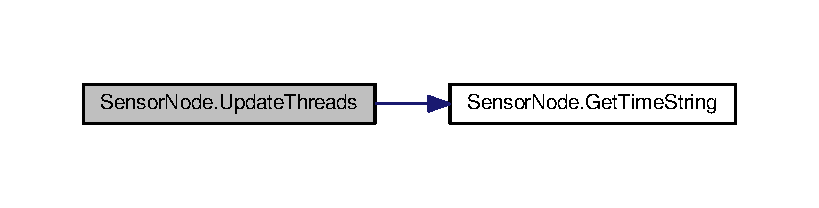
\includegraphics[width=350pt]{namespaceSensorNode_a12355791e34f3144948a5a6f35a3b2b5_cgraph}
\end{center}
\end{figure}




\subsection{Variable Documentation}
\index{Sensor\+Node@{Sensor\+Node}!app@{app}}
\index{app@{app}!Sensor\+Node@{Sensor\+Node}}
\subsubsection[{\texorpdfstring{app}{app}}]{\setlength{\rightskip}{0pt plus 5cm}Sensor\+Node.\+app = {\bf Sensor\+Node}()}\hypertarget{namespaceSensorNode_a1c06b14e3f48f507247d5b8e0e910f35}{}\label{namespaceSensorNode_a1c06b14e3f48f507247d5b8e0e910f35}
\index{Sensor\+Node@{Sensor\+Node}!count@{count}}
\index{count@{count}!Sensor\+Node@{Sensor\+Node}}
\subsubsection[{\texorpdfstring{count}{count}}]{\setlength{\rightskip}{0pt plus 5cm}int Sensor\+Node.\+count = 0}\hypertarget{namespaceSensorNode_a3016284326d74dfe31b9e2ecfa7fa6df}{}\label{namespaceSensorNode_a3016284326d74dfe31b9e2ecfa7fa6df}
\index{Sensor\+Node@{Sensor\+Node}!lock@{lock}}
\index{lock@{lock}!Sensor\+Node@{Sensor\+Node}}
\subsubsection[{\texorpdfstring{lock}{lock}}]{\setlength{\rightskip}{0pt plus 5cm}Sensor\+Node.\+lock = threading.\+Lock()}\hypertarget{namespaceSensorNode_a07847a51e8fc73f94d1b5244eabe2926}{}\label{namespaceSensorNode_a07847a51e8fc73f94d1b5244eabe2926}
\index{Sensor\+Node@{Sensor\+Node}!thr@{thr}}
\index{thr@{thr}!Sensor\+Node@{Sensor\+Node}}
\subsubsection[{\texorpdfstring{thr}{thr}}]{\setlength{\rightskip}{0pt plus 5cm}list Sensor\+Node.\+thr = \mbox{[}$\,$\mbox{]}}\hypertarget{namespaceSensorNode_a972db98176c0c5ca50407768608addd0}{}\label{namespaceSensorNode_a972db98176c0c5ca50407768608addd0}

\hypertarget{namespacesensors}{}\section{sensors Namespace Reference}
\label{namespacesensors}\index{sensors@{sensors}}
\subsection*{Classes}
\begin{DoxyCompactItemize}
\item 
class \hyperlink{classsensors_1_1BMP180}{B\+M\+P180}
\item 
class \hyperlink{classsensors_1_1DHT22}{D\+H\+T22}
\item 
class \hyperlink{classsensors_1_1DS18B20}{D\+S18\+B20}
\item 
class \hyperlink{classsensors_1_1LightAnalog}{Light\+Analog}
\item 
class \hyperlink{classsensors_1_1LightDigital}{Light\+Digital}
\item 
class \hyperlink{classsensors_1_1Movement}{Movement}
\item 
class \hyperlink{classsensors_1_1Sensors}{Sensors}
\end{DoxyCompactItemize}

\hypertarget{namespaceserialconnection}{}\section{serialconnection Namespace Reference}
\label{namespaceserialconnection}\index{serialconnection@{serialconnection}}
\subsection*{Classes}
\begin{DoxyCompactItemize}
\item 
class \hyperlink{classserialconnection_1_1SerialConnection}{Serial\+Connection}
\end{DoxyCompactItemize}

\chapter{Class Documentation}
\hypertarget{classBMP180}{}\section{B\+M\+P180 Class Reference}
\label{classBMP180}\index{B\+M\+P180@{B\+M\+P180}}


{\ttfamily \#include $<$B\+M\+P180.\+hpp$>$}

\subsection*{Public Member Functions}
\begin{DoxyCompactItemize}
\item 
\hyperlink{classBMP180_a8c3e89c7ea65e49c0001a43af07b7c35}{B\+M\+P180} ()
\item 
virtual \hyperlink{classBMP180_a8d434a3074ba607d2dbc14657ae224dd}{$\sim$\+B\+M\+P180} ()
\item 
void \hyperlink{classBMP180_a4a5650b6821c73b5ad9654a9765a9d82}{Init} ()
\end{DoxyCompactItemize}


\subsection{Detailed Description}
\hyperlink{BMP180_8hpp}{B\+M\+P180.\+hpp}

Created on\+: 27 Mar 2017 Author\+: Matthias Minx 

\subsection{Constructor \& Destructor Documentation}
\index{B\+M\+P180@{B\+M\+P180}!B\+M\+P180@{B\+M\+P180}}
\index{B\+M\+P180@{B\+M\+P180}!B\+M\+P180@{B\+M\+P180}}
\subsubsection[{\texorpdfstring{B\+M\+P180()}{BMP180()}}]{\setlength{\rightskip}{0pt plus 5cm}B\+M\+P180\+::\+B\+M\+P180 (
\begin{DoxyParamCaption}
{}
\end{DoxyParamCaption}
)}\hypertarget{classBMP180_a8c3e89c7ea65e49c0001a43af07b7c35}{}\label{classBMP180_a8c3e89c7ea65e49c0001a43af07b7c35}
\index{B\+M\+P180@{B\+M\+P180}!````~B\+M\+P180@{$\sim$\+B\+M\+P180}}
\index{````~B\+M\+P180@{$\sim$\+B\+M\+P180}!B\+M\+P180@{B\+M\+P180}}
\subsubsection[{\texorpdfstring{$\sim$\+B\+M\+P180()}{~BMP180()}}]{\setlength{\rightskip}{0pt plus 5cm}B\+M\+P180\+::$\sim$\+B\+M\+P180 (
\begin{DoxyParamCaption}
{}
\end{DoxyParamCaption}
)\hspace{0.3cm}{\ttfamily [virtual]}}\hypertarget{classBMP180_a8d434a3074ba607d2dbc14657ae224dd}{}\label{classBMP180_a8d434a3074ba607d2dbc14657ae224dd}


\subsection{Member Function Documentation}
\index{B\+M\+P180@{B\+M\+P180}!Init@{Init}}
\index{Init@{Init}!B\+M\+P180@{B\+M\+P180}}
\subsubsection[{\texorpdfstring{Init()}{Init()}}]{\setlength{\rightskip}{0pt plus 5cm}void B\+M\+P180\+::\+Init (
\begin{DoxyParamCaption}
{}
\end{DoxyParamCaption}
)}\hypertarget{classBMP180_a4a5650b6821c73b5ad9654a9765a9d82}{}\label{classBMP180_a4a5650b6821c73b5ad9654a9765a9d82}


The documentation for this class was generated from the following files\+:\begin{DoxyCompactItemize}
\item 
src/\+Sensors/\hyperlink{BMP180_8hpp}{B\+M\+P180.\+hpp}\item 
src/\+Sensors/\hyperlink{BMP180_8cpp}{B\+M\+P180.\+cpp}\end{DoxyCompactItemize}

\hypertarget{classsensors_1_1BMP180}{}\section{sensors.\+B\+M\+P180 Class Reference}
\label{classsensors_1_1BMP180}\index{sensors.\+B\+M\+P180@{sensors.\+B\+M\+P180}}


Inheritance diagram for sensors.\+B\+M\+P180\+:\nopagebreak
\begin{figure}[H]
\begin{center}
\leavevmode
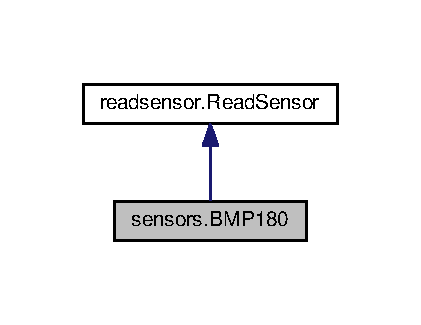
\includegraphics[width=202pt]{classsensors_1_1BMP180__inherit__graph}
\end{center}
\end{figure}


Collaboration diagram for sensors.\+B\+M\+P180\+:\nopagebreak
\begin{figure}[H]
\begin{center}
\leavevmode
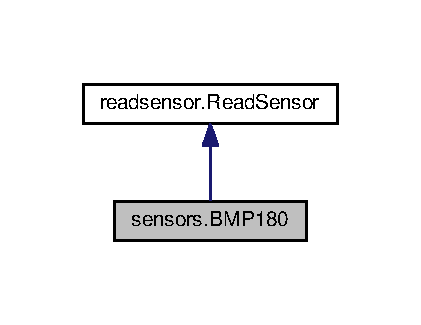
\includegraphics[width=202pt]{classsensors_1_1BMP180__coll__graph}
\end{center}
\end{figure}
\subsection*{Public Member Functions}
\begin{DoxyCompactItemize}
\item 
def \hyperlink{classsensors_1_1BMP180_a4818f2b88b0969dc27a026b901564035}{\+\_\+\+\_\+init\+\_\+\+\_\+} (self, prt, bdrate)
\item 
def \hyperlink{classsensors_1_1BMP180_ad249a90be7cff513ac5a9851a9968403}{Interpret\+Response} (self)
\item 
def \hyperlink{classsensors_1_1BMP180_a5f5a28a84b1e4aac10f9ce814730c9b4}{\+\_\+\+\_\+str\+\_\+\+\_\+} (self)
\end{DoxyCompactItemize}
\subsection*{Public Attributes}
\begin{DoxyCompactItemize}
\item 
\hyperlink{classsensors_1_1BMP180_a455436ba3d7ef32e8e48d69cc84cd345}{P}
\item 
\hyperlink{classsensors_1_1BMP180_a3646abe1f61aa50d15047f09588a2be1}{unitP}
\item 
\hyperlink{classsensors_1_1BMP180_a2063dc8bbcdbe07979e3faf2f6e8eb7d}{T}
\item 
\hyperlink{classsensors_1_1BMP180_a954ddd1f76899d7d2b05aed669abd094}{unitT}
\item 
\hyperlink{classsensors_1_1BMP180_ab0306517f05fca719940e5ac1e129fc3}{err}
\item 
\hyperlink{classsensors_1_1BMP180_ad3ff4c7dc983b1debdb38f9c660f55b9}{node\+M\+AC}
\item 
\hyperlink{classsensors_1_1BMP180_a9ab7d3dda10fdc56600acf177bb044d2}{cmd\+ID}
\item 
\hyperlink{classsensors_1_1BMP180_a8af1eb779b2df113b788bac02d48a592}{p\+String}
\item 
\hyperlink{classsensors_1_1BMP180_a9c885621176fba2aa3760f16e7545fd7}{resp\+Mask}
\end{DoxyCompactItemize}


\subsection{Constructor \& Destructor Documentation}
\index{sensors\+::\+B\+M\+P180@{sensors\+::\+B\+M\+P180}!\+\_\+\+\_\+init\+\_\+\+\_\+@{\+\_\+\+\_\+init\+\_\+\+\_\+}}
\index{\+\_\+\+\_\+init\+\_\+\+\_\+@{\+\_\+\+\_\+init\+\_\+\+\_\+}!sensors\+::\+B\+M\+P180@{sensors\+::\+B\+M\+P180}}
\subsubsection[{\texorpdfstring{\+\_\+\+\_\+init\+\_\+\+\_\+(self, prt, bdrate)}{__init__(self, prt, bdrate)}}]{\setlength{\rightskip}{0pt plus 5cm}def sensors.\+B\+M\+P180.\+\_\+\+\_\+init\+\_\+\+\_\+ (
\begin{DoxyParamCaption}
\item[{}]{self, }
\item[{}]{prt, }
\item[{}]{bdrate}
\end{DoxyParamCaption}
)}\hypertarget{classsensors_1_1BMP180_a4818f2b88b0969dc27a026b901564035}{}\label{classsensors_1_1BMP180_a4818f2b88b0969dc27a026b901564035}


Here is the call graph for this function\+:\nopagebreak
\begin{figure}[H]
\begin{center}
\leavevmode
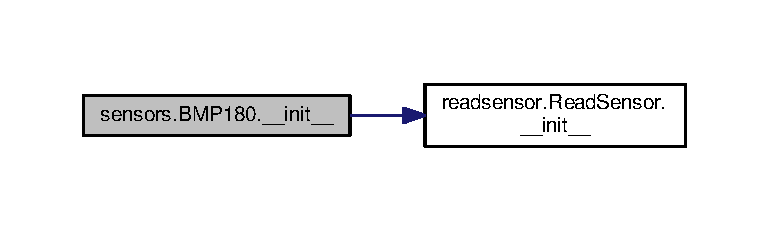
\includegraphics[width=350pt]{classsensors_1_1BMP180_a4818f2b88b0969dc27a026b901564035_cgraph}
\end{center}
\end{figure}




\subsection{Member Function Documentation}
\index{sensors\+::\+B\+M\+P180@{sensors\+::\+B\+M\+P180}!\+\_\+\+\_\+str\+\_\+\+\_\+@{\+\_\+\+\_\+str\+\_\+\+\_\+}}
\index{\+\_\+\+\_\+str\+\_\+\+\_\+@{\+\_\+\+\_\+str\+\_\+\+\_\+}!sensors\+::\+B\+M\+P180@{sensors\+::\+B\+M\+P180}}
\subsubsection[{\texorpdfstring{\+\_\+\+\_\+str\+\_\+\+\_\+(self)}{__str__(self)}}]{\setlength{\rightskip}{0pt plus 5cm}def sensors.\+B\+M\+P180.\+\_\+\+\_\+str\+\_\+\+\_\+ (
\begin{DoxyParamCaption}
\item[{}]{self}
\end{DoxyParamCaption}
)}\hypertarget{classsensors_1_1BMP180_a5f5a28a84b1e4aac10f9ce814730c9b4}{}\label{classsensors_1_1BMP180_a5f5a28a84b1e4aac10f9ce814730c9b4}
\index{sensors\+::\+B\+M\+P180@{sensors\+::\+B\+M\+P180}!Interpret\+Response@{Interpret\+Response}}
\index{Interpret\+Response@{Interpret\+Response}!sensors\+::\+B\+M\+P180@{sensors\+::\+B\+M\+P180}}
\subsubsection[{\texorpdfstring{Interpret\+Response(self)}{InterpretResponse(self)}}]{\setlength{\rightskip}{0pt plus 5cm}def sensors.\+B\+M\+P180.\+Interpret\+Response (
\begin{DoxyParamCaption}
\item[{}]{self}
\end{DoxyParamCaption}
)}\hypertarget{classsensors_1_1BMP180_ad249a90be7cff513ac5a9851a9968403}{}\label{classsensors_1_1BMP180_ad249a90be7cff513ac5a9851a9968403}
\begin{DoxyVerb}Interpret response list \end{DoxyVerb}
 

\subsection{Member Data Documentation}
\index{sensors\+::\+B\+M\+P180@{sensors\+::\+B\+M\+P180}!cmd\+ID@{cmd\+ID}}
\index{cmd\+ID@{cmd\+ID}!sensors\+::\+B\+M\+P180@{sensors\+::\+B\+M\+P180}}
\subsubsection[{\texorpdfstring{cmd\+ID}{cmdID}}]{\setlength{\rightskip}{0pt plus 5cm}sensors.\+B\+M\+P180.\+cmd\+ID}\hypertarget{classsensors_1_1BMP180_a9ab7d3dda10fdc56600acf177bb044d2}{}\label{classsensors_1_1BMP180_a9ab7d3dda10fdc56600acf177bb044d2}
\index{sensors\+::\+B\+M\+P180@{sensors\+::\+B\+M\+P180}!err@{err}}
\index{err@{err}!sensors\+::\+B\+M\+P180@{sensors\+::\+B\+M\+P180}}
\subsubsection[{\texorpdfstring{err}{err}}]{\setlength{\rightskip}{0pt plus 5cm}sensors.\+B\+M\+P180.\+err}\hypertarget{classsensors_1_1BMP180_ab0306517f05fca719940e5ac1e129fc3}{}\label{classsensors_1_1BMP180_ab0306517f05fca719940e5ac1e129fc3}
\index{sensors\+::\+B\+M\+P180@{sensors\+::\+B\+M\+P180}!node\+M\+AC@{node\+M\+AC}}
\index{node\+M\+AC@{node\+M\+AC}!sensors\+::\+B\+M\+P180@{sensors\+::\+B\+M\+P180}}
\subsubsection[{\texorpdfstring{node\+M\+AC}{nodeMAC}}]{\setlength{\rightskip}{0pt plus 5cm}sensors.\+B\+M\+P180.\+node\+M\+AC}\hypertarget{classsensors_1_1BMP180_ad3ff4c7dc983b1debdb38f9c660f55b9}{}\label{classsensors_1_1BMP180_ad3ff4c7dc983b1debdb38f9c660f55b9}
\index{sensors\+::\+B\+M\+P180@{sensors\+::\+B\+M\+P180}!P@{P}}
\index{P@{P}!sensors\+::\+B\+M\+P180@{sensors\+::\+B\+M\+P180}}
\subsubsection[{\texorpdfstring{P}{P}}]{\setlength{\rightskip}{0pt plus 5cm}sensors.\+B\+M\+P180.\+P}\hypertarget{classsensors_1_1BMP180_a455436ba3d7ef32e8e48d69cc84cd345}{}\label{classsensors_1_1BMP180_a455436ba3d7ef32e8e48d69cc84cd345}
\index{sensors\+::\+B\+M\+P180@{sensors\+::\+B\+M\+P180}!p\+String@{p\+String}}
\index{p\+String@{p\+String}!sensors\+::\+B\+M\+P180@{sensors\+::\+B\+M\+P180}}
\subsubsection[{\texorpdfstring{p\+String}{pString}}]{\setlength{\rightskip}{0pt plus 5cm}sensors.\+B\+M\+P180.\+p\+String}\hypertarget{classsensors_1_1BMP180_a8af1eb779b2df113b788bac02d48a592}{}\label{classsensors_1_1BMP180_a8af1eb779b2df113b788bac02d48a592}
\index{sensors\+::\+B\+M\+P180@{sensors\+::\+B\+M\+P180}!resp\+Mask@{resp\+Mask}}
\index{resp\+Mask@{resp\+Mask}!sensors\+::\+B\+M\+P180@{sensors\+::\+B\+M\+P180}}
\subsubsection[{\texorpdfstring{resp\+Mask}{respMask}}]{\setlength{\rightskip}{0pt plus 5cm}sensors.\+B\+M\+P180.\+resp\+Mask}\hypertarget{classsensors_1_1BMP180_a9c885621176fba2aa3760f16e7545fd7}{}\label{classsensors_1_1BMP180_a9c885621176fba2aa3760f16e7545fd7}
\index{sensors\+::\+B\+M\+P180@{sensors\+::\+B\+M\+P180}!T@{T}}
\index{T@{T}!sensors\+::\+B\+M\+P180@{sensors\+::\+B\+M\+P180}}
\subsubsection[{\texorpdfstring{T}{T}}]{\setlength{\rightskip}{0pt plus 5cm}sensors.\+B\+M\+P180.\+T}\hypertarget{classsensors_1_1BMP180_a2063dc8bbcdbe07979e3faf2f6e8eb7d}{}\label{classsensors_1_1BMP180_a2063dc8bbcdbe07979e3faf2f6e8eb7d}
\index{sensors\+::\+B\+M\+P180@{sensors\+::\+B\+M\+P180}!unitP@{unitP}}
\index{unitP@{unitP}!sensors\+::\+B\+M\+P180@{sensors\+::\+B\+M\+P180}}
\subsubsection[{\texorpdfstring{unitP}{unitP}}]{\setlength{\rightskip}{0pt plus 5cm}sensors.\+B\+M\+P180.\+unitP}\hypertarget{classsensors_1_1BMP180_a3646abe1f61aa50d15047f09588a2be1}{}\label{classsensors_1_1BMP180_a3646abe1f61aa50d15047f09588a2be1}
\index{sensors\+::\+B\+M\+P180@{sensors\+::\+B\+M\+P180}!unitT@{unitT}}
\index{unitT@{unitT}!sensors\+::\+B\+M\+P180@{sensors\+::\+B\+M\+P180}}
\subsubsection[{\texorpdfstring{unitT}{unitT}}]{\setlength{\rightskip}{0pt plus 5cm}sensors.\+B\+M\+P180.\+unitT}\hypertarget{classsensors_1_1BMP180_a954ddd1f76899d7d2b05aed669abd094}{}\label{classsensors_1_1BMP180_a954ddd1f76899d7d2b05aed669abd094}


The documentation for this class was generated from the following file\+:\begin{DoxyCompactItemize}
\item 
Python/\hyperlink{sensors_8py}{sensors.\+py}\end{DoxyCompactItemize}

\hypertarget{classDHT22}{}\section{D\+H\+T22 Class Reference}
\label{classDHT22}\index{D\+H\+T22@{D\+H\+T22}}


{\ttfamily \#include $<$D\+H\+T22.\+h$>$}

\subsection*{Public Member Functions}
\begin{DoxyCompactItemize}
\item 
\hyperlink{classDHT22_ad80f0ddc323aa1ec6702230d4a80349f}{D\+H\+T22} ()
\item 
\hyperlink{classDHT22_a266c5c8555486bb830dc4668cd1875d4}{D\+H\+T22} (volatile uint8\+\_\+t \&Wire\+\_\+\+P\+O\+RT, volatile uint8\+\_\+t \&Wire\+\_\+\+D\+DR, volatile uint8\+\_\+t \&Wire\+\_\+\+P\+IN, uint8\+\_\+t Wire\+\_\+\+DQ)
\item 
int8\+\_\+t \hyperlink{classDHT22_a51552e5b7373329a6751aeffc04a8fd5}{Get\+Temperature\+Humidity} (float $\ast$temperature, float $\ast$humidity)
\item 
int8\+\_\+t \hyperlink{classDHT22_abe301571f40deb569b74e980ef2da9a7}{Get\+Temperature} (float $\ast$temperature)
\item 
int8\+\_\+t \hyperlink{classDHT22_acaffb8b6e2602a291d3b2e2ec5bc340c}{Get\+Humidity} (float $\ast$humidity)
\item 
void \hyperlink{classDHT22_ac3f4e0757e14c5a8ea96cd4eb5e8d57c}{Get\+Sensor\+String\+X\+ML} (char $\ast$string)
\item 
void \hyperlink{classDHT22_a7384e5b3512bca9692932cbc74c0d110}{Get\+Sensor\+Temperature\+String\+X\+ML} (char $\ast$string)
\item 
void \hyperlink{classDHT22_acee19cfc832183328130ec99ce0f9854}{Get\+Sensor\+Humidity\+String\+X\+ML} (char $\ast$string)
\end{DoxyCompactItemize}
\subsection*{Private Member Functions}
\begin{DoxyCompactItemize}
\item 
void \hyperlink{classDHT22_acfa5b6640685318856f09aa84080fd76}{Reset} ()
\item 
uint8\+\_\+t \hyperlink{classDHT22_acf1337337af198d3a6216f625c70cbc7}{Send\+Request} (uint8\+\_\+t bit)
\item 
int8\+\_\+t \hyperlink{classDHT22_ae8fbd3966b285fd9b7318dcad2036e93}{Get\+Data} (float $\ast$temperature, float $\ast$humidity)
\item 
void \hyperlink{classDHT22_aae1d3f75d7a34843d3a4b533c56e474c}{A\+M2302\+\_\+\+P\+I\+N\+\_\+\+I\+N\+P\+U\+T\+\_\+\+M\+O\+DE} ()
\item 
void \hyperlink{classDHT22_a96e379a2cf2c6239253c9f706959253c}{A\+M2302\+\_\+\+P\+I\+N\+\_\+\+O\+U\+T\+P\+U\+T\+\_\+\+M\+O\+DE} ()
\item 
void \hyperlink{classDHT22_a312eb760672d2818f8de68c553bd5a21}{A\+M2302\+\_\+\+P\+I\+N\+\_\+\+L\+OW} ()
\item 
void \hyperlink{classDHT22_a98ca5e15fa219b57e819691e16707122}{A\+M2302\+\_\+\+P\+I\+N\+\_\+\+H\+I\+GH} ()
\item 
bool \hyperlink{classDHT22_ae2f4f7c34bf80cd3f4bf0da52fa96572}{A\+M2302\+\_\+\+H\+I\+G\+H\+\_\+\+I\+N\+P\+UT} ()
\end{DoxyCompactItemize}
\subsection*{Private Attributes}
\begin{DoxyCompactItemize}
\item 
volatile uint8\+\_\+t $\ast$ \hyperlink{classDHT22_a0966fbe5db17d7ca6f1f036830e27502}{A\+M2302\+\_\+\+W\+I\+R\+E\+\_\+\+P\+O\+RT}
\item 
volatile uint8\+\_\+t $\ast$ \hyperlink{classDHT22_a69649c4246cd4e255a6e61961b0c948b}{A\+M2302\+\_\+\+W\+I\+R\+E\+\_\+\+D\+DR}
\item 
volatile uint8\+\_\+t $\ast$ \hyperlink{classDHT22_a5555aa8aa95149f3a3723582bb4ceffa}{A\+M2302\+\_\+\+W\+I\+R\+E\+\_\+\+P\+IN}
\item 
uint8\+\_\+t \hyperlink{classDHT22_a4b6de6908e5eb743dec2c254ef89782e}{A\+M2302\+\_\+\+W\+I\+R\+E\+\_\+\+DQ}
\item 
uint8\+\_\+t \hyperlink{classDHT22_acbca744f7ed6f46e2d060c7047b0b1a4}{T\+I\+M\+E\+O\+UT}
\end{DoxyCompactItemize}


\subsection{Constructor \& Destructor Documentation}
\index{D\+H\+T22@{D\+H\+T22}!D\+H\+T22@{D\+H\+T22}}
\index{D\+H\+T22@{D\+H\+T22}!D\+H\+T22@{D\+H\+T22}}
\subsubsection[{\texorpdfstring{D\+H\+T22()}{DHT22()}}]{\setlength{\rightskip}{0pt plus 5cm}D\+H\+T22\+::\+D\+H\+T22 (
\begin{DoxyParamCaption}
{}
\end{DoxyParamCaption}
)}\hypertarget{classDHT22_ad80f0ddc323aa1ec6702230d4a80349f}{}\label{classDHT22_ad80f0ddc323aa1ec6702230d4a80349f}
\index{D\+H\+T22@{D\+H\+T22}!D\+H\+T22@{D\+H\+T22}}
\index{D\+H\+T22@{D\+H\+T22}!D\+H\+T22@{D\+H\+T22}}
\subsubsection[{\texorpdfstring{D\+H\+T22(volatile uint8\+\_\+t \&\+Wire\+\_\+\+P\+O\+R\+T, volatile uint8\+\_\+t \&\+Wire\+\_\+\+D\+D\+R, volatile uint8\+\_\+t \&\+Wire\+\_\+\+P\+I\+N, uint8\+\_\+t Wire\+\_\+\+D\+Q)}{DHT22(volatile uint8_t &Wire_PORT, volatile uint8_t &Wire_DDR, volatile uint8_t &Wire_PIN, uint8_t Wire_DQ)}}]{\setlength{\rightskip}{0pt plus 5cm}D\+H\+T22\+::\+D\+H\+T22 (
\begin{DoxyParamCaption}
\item[{volatile uint8\+\_\+t \&}]{Wire\+\_\+\+P\+O\+RT, }
\item[{volatile uint8\+\_\+t \&}]{Wire\+\_\+\+D\+DR, }
\item[{volatile uint8\+\_\+t \&}]{Wire\+\_\+\+P\+IN, }
\item[{uint8\+\_\+t}]{Wire\+\_\+\+DQ}
\end{DoxyParamCaption}
)}\hypertarget{classDHT22_a266c5c8555486bb830dc4668cd1875d4}{}\label{classDHT22_a266c5c8555486bb830dc4668cd1875d4}


\subsection{Member Function Documentation}
\index{D\+H\+T22@{D\+H\+T22}!A\+M2302\+\_\+\+H\+I\+G\+H\+\_\+\+I\+N\+P\+UT@{A\+M2302\+\_\+\+H\+I\+G\+H\+\_\+\+I\+N\+P\+UT}}
\index{A\+M2302\+\_\+\+H\+I\+G\+H\+\_\+\+I\+N\+P\+UT@{A\+M2302\+\_\+\+H\+I\+G\+H\+\_\+\+I\+N\+P\+UT}!D\+H\+T22@{D\+H\+T22}}
\subsubsection[{\texorpdfstring{A\+M2302\+\_\+\+H\+I\+G\+H\+\_\+\+I\+N\+P\+U\+T()}{AM2302_HIGH_INPUT()}}]{\setlength{\rightskip}{0pt plus 5cm}bool D\+H\+T22\+::\+A\+M2302\+\_\+\+H\+I\+G\+H\+\_\+\+I\+N\+P\+UT (
\begin{DoxyParamCaption}
{}
\end{DoxyParamCaption}
)\hspace{0.3cm}{\ttfamily [inline]}, {\ttfamily [private]}}\hypertarget{classDHT22_ae2f4f7c34bf80cd3f4bf0da52fa96572}{}\label{classDHT22_ae2f4f7c34bf80cd3f4bf0da52fa96572}
\index{D\+H\+T22@{D\+H\+T22}!A\+M2302\+\_\+\+P\+I\+N\+\_\+\+H\+I\+GH@{A\+M2302\+\_\+\+P\+I\+N\+\_\+\+H\+I\+GH}}
\index{A\+M2302\+\_\+\+P\+I\+N\+\_\+\+H\+I\+GH@{A\+M2302\+\_\+\+P\+I\+N\+\_\+\+H\+I\+GH}!D\+H\+T22@{D\+H\+T22}}
\subsubsection[{\texorpdfstring{A\+M2302\+\_\+\+P\+I\+N\+\_\+\+H\+I\+G\+H()}{AM2302_PIN_HIGH()}}]{\setlength{\rightskip}{0pt plus 5cm}void D\+H\+T22\+::\+A\+M2302\+\_\+\+P\+I\+N\+\_\+\+H\+I\+GH (
\begin{DoxyParamCaption}
{}
\end{DoxyParamCaption}
)\hspace{0.3cm}{\ttfamily [inline]}, {\ttfamily [private]}}\hypertarget{classDHT22_a98ca5e15fa219b57e819691e16707122}{}\label{classDHT22_a98ca5e15fa219b57e819691e16707122}
\index{D\+H\+T22@{D\+H\+T22}!A\+M2302\+\_\+\+P\+I\+N\+\_\+\+I\+N\+P\+U\+T\+\_\+\+M\+O\+DE@{A\+M2302\+\_\+\+P\+I\+N\+\_\+\+I\+N\+P\+U\+T\+\_\+\+M\+O\+DE}}
\index{A\+M2302\+\_\+\+P\+I\+N\+\_\+\+I\+N\+P\+U\+T\+\_\+\+M\+O\+DE@{A\+M2302\+\_\+\+P\+I\+N\+\_\+\+I\+N\+P\+U\+T\+\_\+\+M\+O\+DE}!D\+H\+T22@{D\+H\+T22}}
\subsubsection[{\texorpdfstring{A\+M2302\+\_\+\+P\+I\+N\+\_\+\+I\+N\+P\+U\+T\+\_\+\+M\+O\+D\+E()}{AM2302_PIN_INPUT_MODE()}}]{\setlength{\rightskip}{0pt plus 5cm}void D\+H\+T22\+::\+A\+M2302\+\_\+\+P\+I\+N\+\_\+\+I\+N\+P\+U\+T\+\_\+\+M\+O\+DE (
\begin{DoxyParamCaption}
{}
\end{DoxyParamCaption}
)\hspace{0.3cm}{\ttfamily [inline]}, {\ttfamily [private]}}\hypertarget{classDHT22_aae1d3f75d7a34843d3a4b533c56e474c}{}\label{classDHT22_aae1d3f75d7a34843d3a4b533c56e474c}
\index{D\+H\+T22@{D\+H\+T22}!A\+M2302\+\_\+\+P\+I\+N\+\_\+\+L\+OW@{A\+M2302\+\_\+\+P\+I\+N\+\_\+\+L\+OW}}
\index{A\+M2302\+\_\+\+P\+I\+N\+\_\+\+L\+OW@{A\+M2302\+\_\+\+P\+I\+N\+\_\+\+L\+OW}!D\+H\+T22@{D\+H\+T22}}
\subsubsection[{\texorpdfstring{A\+M2302\+\_\+\+P\+I\+N\+\_\+\+L\+O\+W()}{AM2302_PIN_LOW()}}]{\setlength{\rightskip}{0pt plus 5cm}void D\+H\+T22\+::\+A\+M2302\+\_\+\+P\+I\+N\+\_\+\+L\+OW (
\begin{DoxyParamCaption}
{}
\end{DoxyParamCaption}
)\hspace{0.3cm}{\ttfamily [inline]}, {\ttfamily [private]}}\hypertarget{classDHT22_a312eb760672d2818f8de68c553bd5a21}{}\label{classDHT22_a312eb760672d2818f8de68c553bd5a21}
\index{D\+H\+T22@{D\+H\+T22}!A\+M2302\+\_\+\+P\+I\+N\+\_\+\+O\+U\+T\+P\+U\+T\+\_\+\+M\+O\+DE@{A\+M2302\+\_\+\+P\+I\+N\+\_\+\+O\+U\+T\+P\+U\+T\+\_\+\+M\+O\+DE}}
\index{A\+M2302\+\_\+\+P\+I\+N\+\_\+\+O\+U\+T\+P\+U\+T\+\_\+\+M\+O\+DE@{A\+M2302\+\_\+\+P\+I\+N\+\_\+\+O\+U\+T\+P\+U\+T\+\_\+\+M\+O\+DE}!D\+H\+T22@{D\+H\+T22}}
\subsubsection[{\texorpdfstring{A\+M2302\+\_\+\+P\+I\+N\+\_\+\+O\+U\+T\+P\+U\+T\+\_\+\+M\+O\+D\+E()}{AM2302_PIN_OUTPUT_MODE()}}]{\setlength{\rightskip}{0pt plus 5cm}void D\+H\+T22\+::\+A\+M2302\+\_\+\+P\+I\+N\+\_\+\+O\+U\+T\+P\+U\+T\+\_\+\+M\+O\+DE (
\begin{DoxyParamCaption}
{}
\end{DoxyParamCaption}
)\hspace{0.3cm}{\ttfamily [inline]}, {\ttfamily [private]}}\hypertarget{classDHT22_a96e379a2cf2c6239253c9f706959253c}{}\label{classDHT22_a96e379a2cf2c6239253c9f706959253c}
\index{D\+H\+T22@{D\+H\+T22}!Get\+Data@{Get\+Data}}
\index{Get\+Data@{Get\+Data}!D\+H\+T22@{D\+H\+T22}}
\subsubsection[{\texorpdfstring{Get\+Data(float $\ast$temperature, float $\ast$humidity)}{GetData(float *temperature, float *humidity)}}]{\setlength{\rightskip}{0pt plus 5cm}int8\+\_\+t D\+H\+T22\+::\+Get\+Data (
\begin{DoxyParamCaption}
\item[{float $\ast$}]{temperature, }
\item[{float $\ast$}]{humidity}
\end{DoxyParamCaption}
)\hspace{0.3cm}{\ttfamily [private]}}\hypertarget{classDHT22_ae8fbd3966b285fd9b7318dcad2036e93}{}\label{classDHT22_ae8fbd3966b285fd9b7318dcad2036e93}


Here is the call graph for this function\+:\nopagebreak
\begin{figure}[H]
\begin{center}
\leavevmode
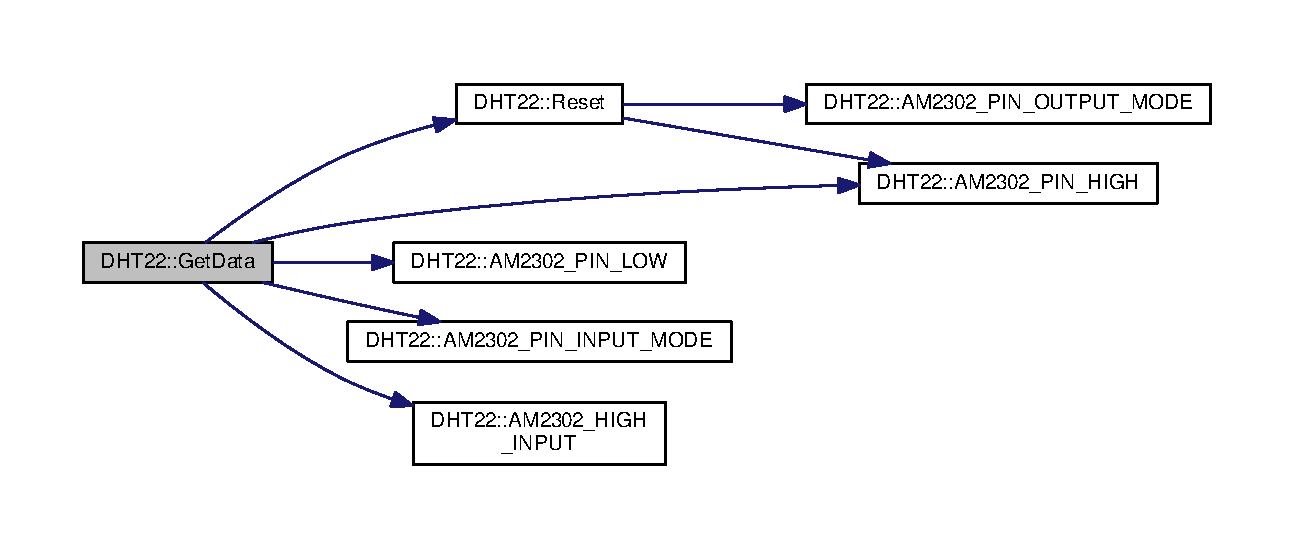
\includegraphics[width=350pt]{classDHT22_ae8fbd3966b285fd9b7318dcad2036e93_cgraph}
\end{center}
\end{figure}


\index{D\+H\+T22@{D\+H\+T22}!Get\+Humidity@{Get\+Humidity}}
\index{Get\+Humidity@{Get\+Humidity}!D\+H\+T22@{D\+H\+T22}}
\subsubsection[{\texorpdfstring{Get\+Humidity(float $\ast$humidity)}{GetHumidity(float *humidity)}}]{\setlength{\rightskip}{0pt plus 5cm}int8\+\_\+t D\+H\+T22\+::\+Get\+Humidity (
\begin{DoxyParamCaption}
\item[{float $\ast$}]{humidity}
\end{DoxyParamCaption}
)}\hypertarget{classDHT22_acaffb8b6e2602a291d3b2e2ec5bc340c}{}\label{classDHT22_acaffb8b6e2602a291d3b2e2ec5bc340c}


Here is the call graph for this function\+:\nopagebreak
\begin{figure}[H]
\begin{center}
\leavevmode
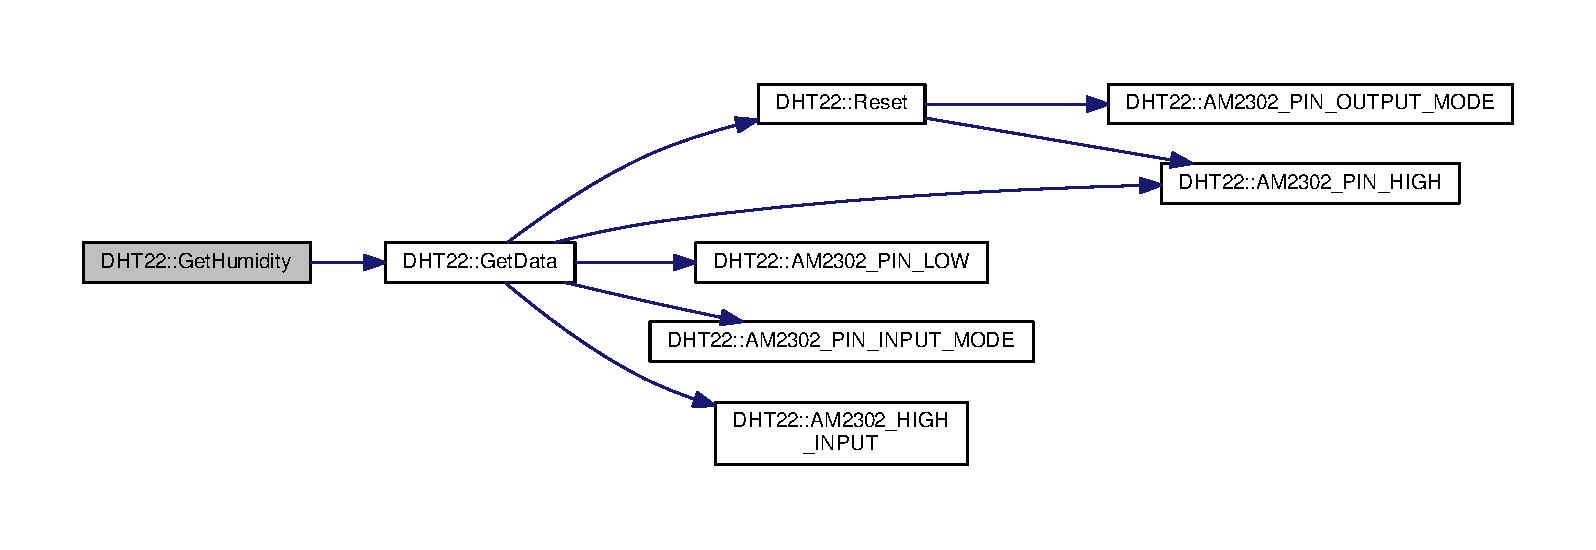
\includegraphics[width=350pt]{classDHT22_acaffb8b6e2602a291d3b2e2ec5bc340c_cgraph}
\end{center}
\end{figure}


\index{D\+H\+T22@{D\+H\+T22}!Get\+Sensor\+Humidity\+String\+X\+ML@{Get\+Sensor\+Humidity\+String\+X\+ML}}
\index{Get\+Sensor\+Humidity\+String\+X\+ML@{Get\+Sensor\+Humidity\+String\+X\+ML}!D\+H\+T22@{D\+H\+T22}}
\subsubsection[{\texorpdfstring{Get\+Sensor\+Humidity\+String\+X\+M\+L(char $\ast$string)}{GetSensorHumidityStringXML(char *string)}}]{\setlength{\rightskip}{0pt plus 5cm}void D\+H\+T22\+::\+Get\+Sensor\+Humidity\+String\+X\+ML (
\begin{DoxyParamCaption}
\item[{char $\ast$}]{string}
\end{DoxyParamCaption}
)}\hypertarget{classDHT22_acee19cfc832183328130ec99ce0f9854}{}\label{classDHT22_acee19cfc832183328130ec99ce0f9854}


Here is the call graph for this function\+:\nopagebreak
\begin{figure}[H]
\begin{center}
\leavevmode
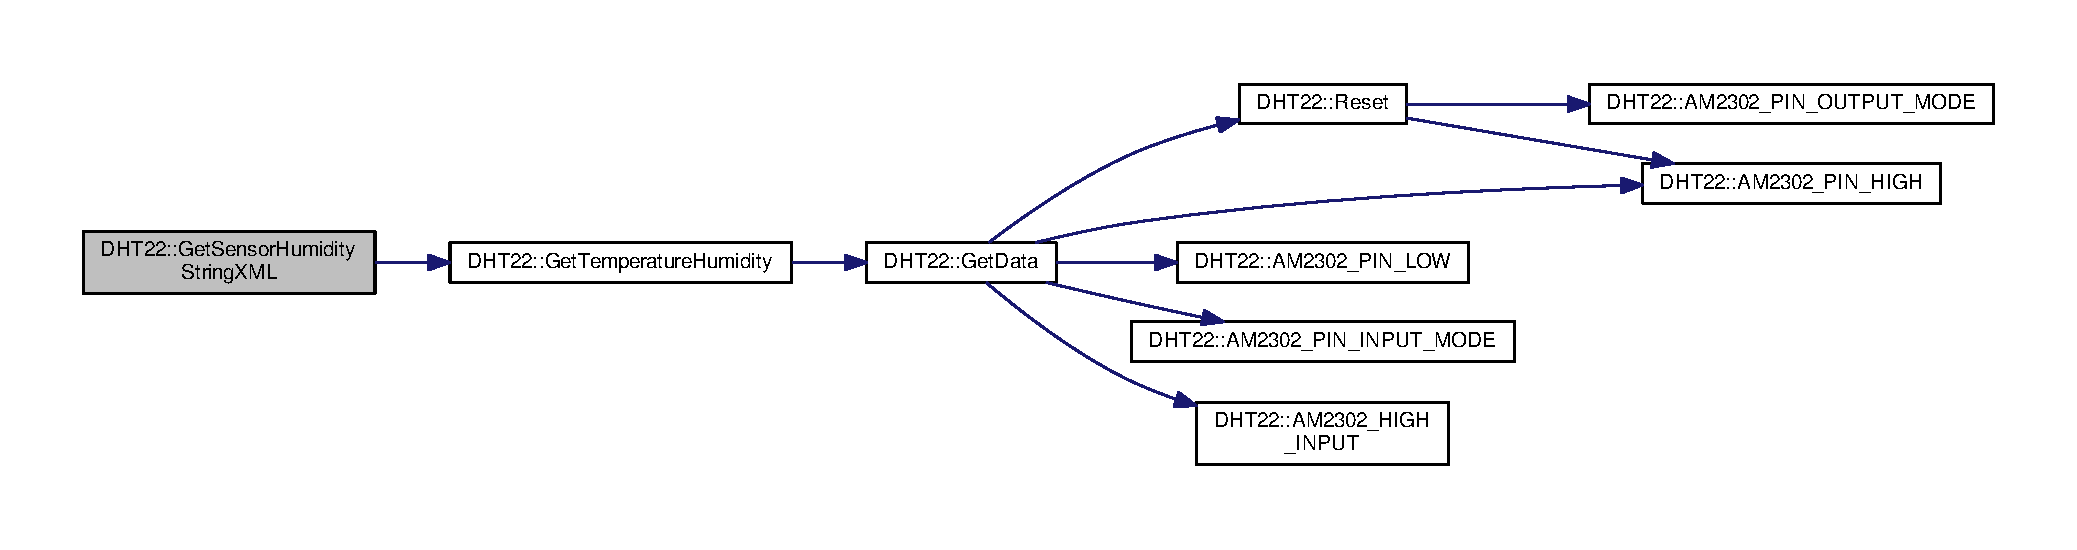
\includegraphics[width=350pt]{classDHT22_acee19cfc832183328130ec99ce0f9854_cgraph}
\end{center}
\end{figure}


\index{D\+H\+T22@{D\+H\+T22}!Get\+Sensor\+String\+X\+ML@{Get\+Sensor\+String\+X\+ML}}
\index{Get\+Sensor\+String\+X\+ML@{Get\+Sensor\+String\+X\+ML}!D\+H\+T22@{D\+H\+T22}}
\subsubsection[{\texorpdfstring{Get\+Sensor\+String\+X\+M\+L(char $\ast$string)}{GetSensorStringXML(char *string)}}]{\setlength{\rightskip}{0pt plus 5cm}void D\+H\+T22\+::\+Get\+Sensor\+String\+X\+ML (
\begin{DoxyParamCaption}
\item[{char $\ast$}]{string}
\end{DoxyParamCaption}
)}\hypertarget{classDHT22_ac3f4e0757e14c5a8ea96cd4eb5e8d57c}{}\label{classDHT22_ac3f4e0757e14c5a8ea96cd4eb5e8d57c}


Here is the call graph for this function\+:\nopagebreak
\begin{figure}[H]
\begin{center}
\leavevmode
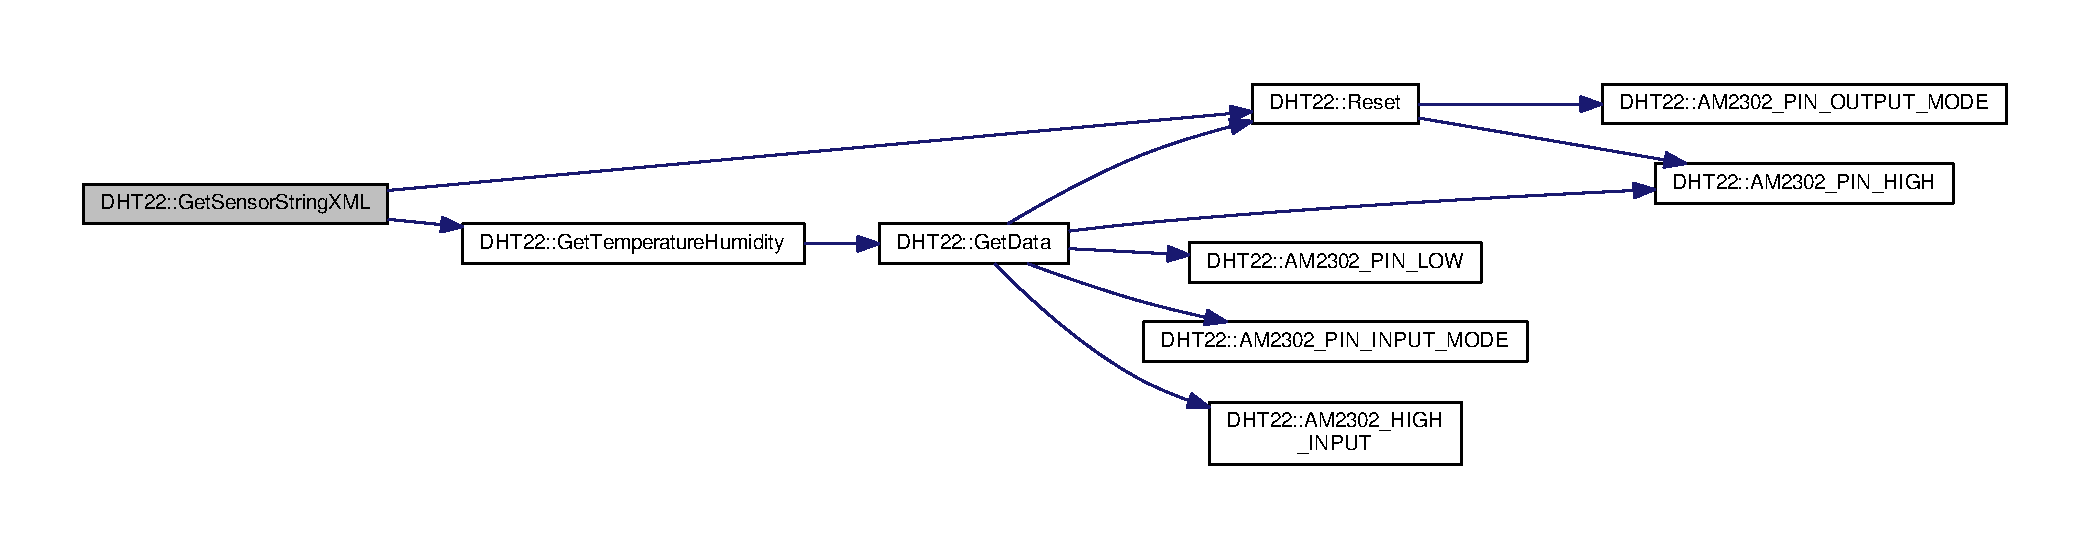
\includegraphics[width=350pt]{classDHT22_ac3f4e0757e14c5a8ea96cd4eb5e8d57c_cgraph}
\end{center}
\end{figure}


\index{D\+H\+T22@{D\+H\+T22}!Get\+Sensor\+Temperature\+String\+X\+ML@{Get\+Sensor\+Temperature\+String\+X\+ML}}
\index{Get\+Sensor\+Temperature\+String\+X\+ML@{Get\+Sensor\+Temperature\+String\+X\+ML}!D\+H\+T22@{D\+H\+T22}}
\subsubsection[{\texorpdfstring{Get\+Sensor\+Temperature\+String\+X\+M\+L(char $\ast$string)}{GetSensorTemperatureStringXML(char *string)}}]{\setlength{\rightskip}{0pt plus 5cm}void D\+H\+T22\+::\+Get\+Sensor\+Temperature\+String\+X\+ML (
\begin{DoxyParamCaption}
\item[{char $\ast$}]{string}
\end{DoxyParamCaption}
)}\hypertarget{classDHT22_a7384e5b3512bca9692932cbc74c0d110}{}\label{classDHT22_a7384e5b3512bca9692932cbc74c0d110}


Here is the call graph for this function\+:\nopagebreak
\begin{figure}[H]
\begin{center}
\leavevmode
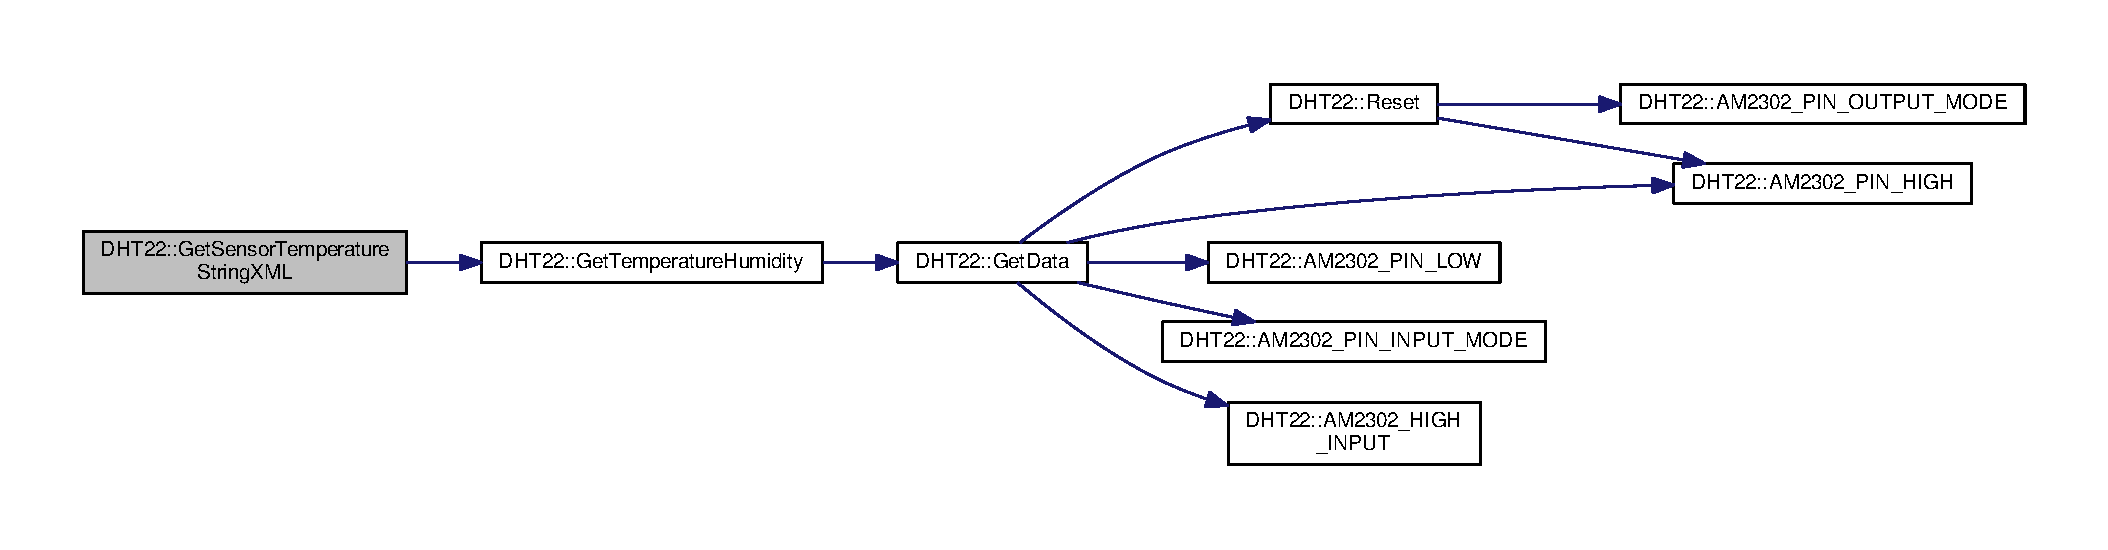
\includegraphics[width=350pt]{classDHT22_a7384e5b3512bca9692932cbc74c0d110_cgraph}
\end{center}
\end{figure}


\index{D\+H\+T22@{D\+H\+T22}!Get\+Temperature@{Get\+Temperature}}
\index{Get\+Temperature@{Get\+Temperature}!D\+H\+T22@{D\+H\+T22}}
\subsubsection[{\texorpdfstring{Get\+Temperature(float $\ast$temperature)}{GetTemperature(float *temperature)}}]{\setlength{\rightskip}{0pt plus 5cm}int8\+\_\+t D\+H\+T22\+::\+Get\+Temperature (
\begin{DoxyParamCaption}
\item[{float $\ast$}]{temperature}
\end{DoxyParamCaption}
)}\hypertarget{classDHT22_abe301571f40deb569b74e980ef2da9a7}{}\label{classDHT22_abe301571f40deb569b74e980ef2da9a7}


Here is the call graph for this function\+:\nopagebreak
\begin{figure}[H]
\begin{center}
\leavevmode
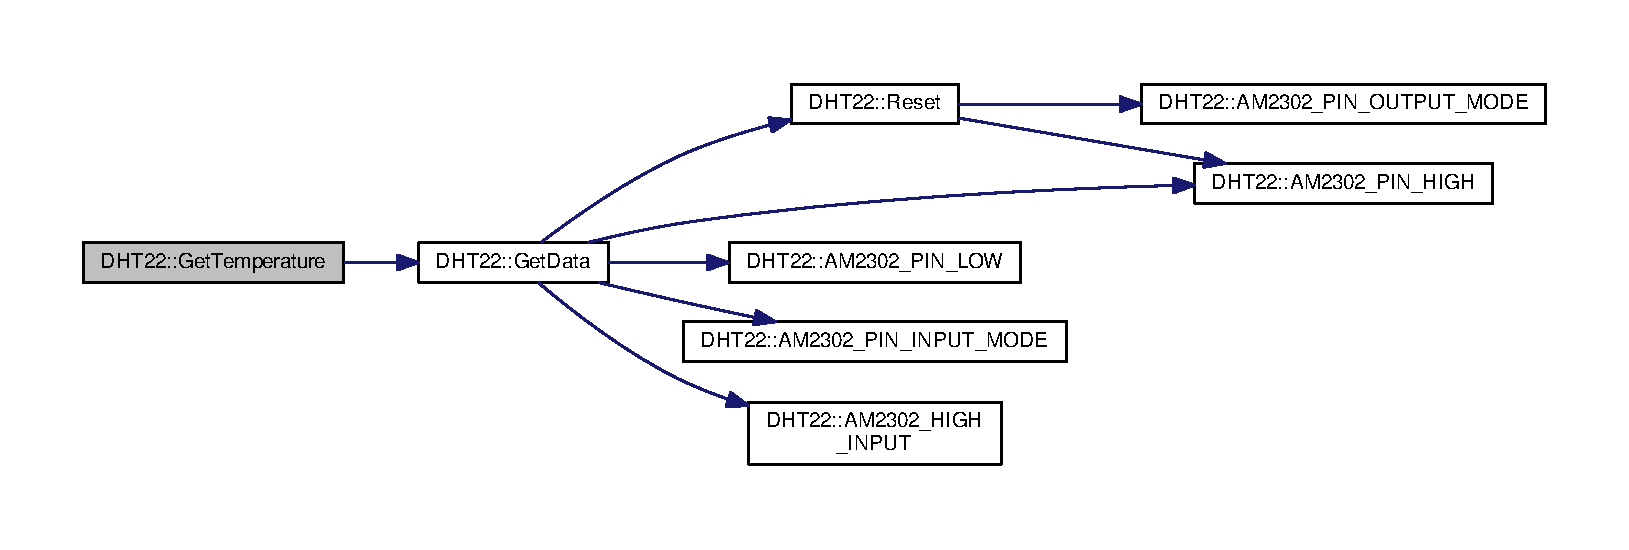
\includegraphics[width=350pt]{classDHT22_abe301571f40deb569b74e980ef2da9a7_cgraph}
\end{center}
\end{figure}


\index{D\+H\+T22@{D\+H\+T22}!Get\+Temperature\+Humidity@{Get\+Temperature\+Humidity}}
\index{Get\+Temperature\+Humidity@{Get\+Temperature\+Humidity}!D\+H\+T22@{D\+H\+T22}}
\subsubsection[{\texorpdfstring{Get\+Temperature\+Humidity(float $\ast$temperature, float $\ast$humidity)}{GetTemperatureHumidity(float *temperature, float *humidity)}}]{\setlength{\rightskip}{0pt plus 5cm}int8\+\_\+t D\+H\+T22\+::\+Get\+Temperature\+Humidity (
\begin{DoxyParamCaption}
\item[{float $\ast$}]{temperature, }
\item[{float $\ast$}]{humidity}
\end{DoxyParamCaption}
)}\hypertarget{classDHT22_a51552e5b7373329a6751aeffc04a8fd5}{}\label{classDHT22_a51552e5b7373329a6751aeffc04a8fd5}


Here is the call graph for this function\+:\nopagebreak
\begin{figure}[H]
\begin{center}
\leavevmode
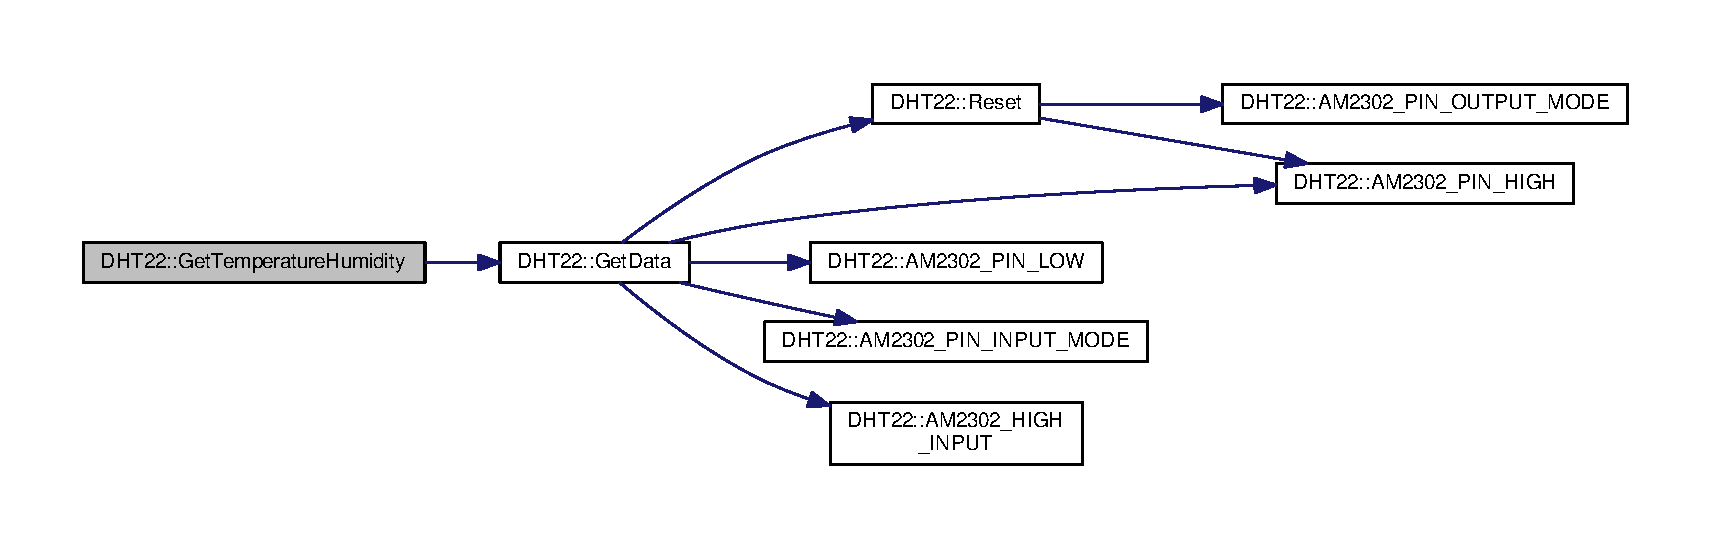
\includegraphics[width=350pt]{classDHT22_a51552e5b7373329a6751aeffc04a8fd5_cgraph}
\end{center}
\end{figure}


\index{D\+H\+T22@{D\+H\+T22}!Reset@{Reset}}
\index{Reset@{Reset}!D\+H\+T22@{D\+H\+T22}}
\subsubsection[{\texorpdfstring{Reset()}{Reset()}}]{\setlength{\rightskip}{0pt plus 5cm}void D\+H\+T22\+::\+Reset (
\begin{DoxyParamCaption}
{}
\end{DoxyParamCaption}
)\hspace{0.3cm}{\ttfamily [private]}}\hypertarget{classDHT22_acfa5b6640685318856f09aa84080fd76}{}\label{classDHT22_acfa5b6640685318856f09aa84080fd76}


Here is the call graph for this function\+:\nopagebreak
\begin{figure}[H]
\begin{center}
\leavevmode
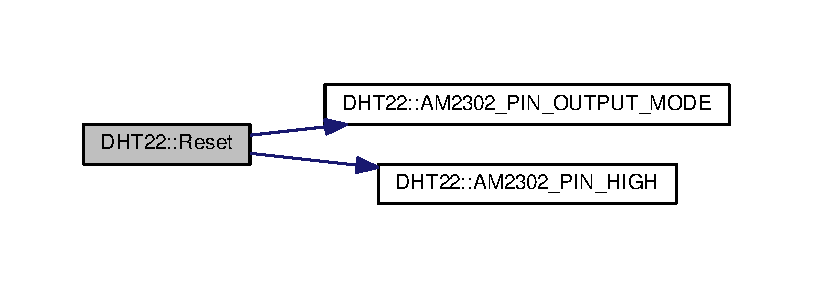
\includegraphics[width=350pt]{classDHT22_acfa5b6640685318856f09aa84080fd76_cgraph}
\end{center}
\end{figure}


\index{D\+H\+T22@{D\+H\+T22}!Send\+Request@{Send\+Request}}
\index{Send\+Request@{Send\+Request}!D\+H\+T22@{D\+H\+T22}}
\subsubsection[{\texorpdfstring{Send\+Request(uint8\+\_\+t bit)}{SendRequest(uint8_t bit)}}]{\setlength{\rightskip}{0pt plus 5cm}uint8\+\_\+t D\+H\+T22\+::\+Send\+Request (
\begin{DoxyParamCaption}
\item[{uint8\+\_\+t}]{bit}
\end{DoxyParamCaption}
)\hspace{0.3cm}{\ttfamily [private]}}\hypertarget{classDHT22_acf1337337af198d3a6216f625c70cbc7}{}\label{classDHT22_acf1337337af198d3a6216f625c70cbc7}


Here is the call graph for this function\+:\nopagebreak
\begin{figure}[H]
\begin{center}
\leavevmode
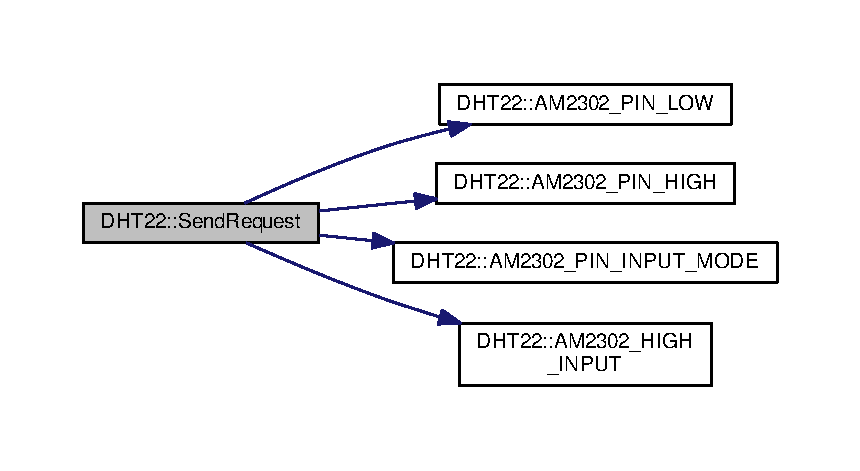
\includegraphics[width=350pt]{classDHT22_acf1337337af198d3a6216f625c70cbc7_cgraph}
\end{center}
\end{figure}




\subsection{Member Data Documentation}
\index{D\+H\+T22@{D\+H\+T22}!A\+M2302\+\_\+\+W\+I\+R\+E\+\_\+\+D\+DR@{A\+M2302\+\_\+\+W\+I\+R\+E\+\_\+\+D\+DR}}
\index{A\+M2302\+\_\+\+W\+I\+R\+E\+\_\+\+D\+DR@{A\+M2302\+\_\+\+W\+I\+R\+E\+\_\+\+D\+DR}!D\+H\+T22@{D\+H\+T22}}
\subsubsection[{\texorpdfstring{A\+M2302\+\_\+\+W\+I\+R\+E\+\_\+\+D\+DR}{AM2302_WIRE_DDR}}]{\setlength{\rightskip}{0pt plus 5cm}volatile uint8\+\_\+t$\ast$ D\+H\+T22\+::\+A\+M2302\+\_\+\+W\+I\+R\+E\+\_\+\+D\+DR\hspace{0.3cm}{\ttfamily [private]}}\hypertarget{classDHT22_a69649c4246cd4e255a6e61961b0c948b}{}\label{classDHT22_a69649c4246cd4e255a6e61961b0c948b}
\index{D\+H\+T22@{D\+H\+T22}!A\+M2302\+\_\+\+W\+I\+R\+E\+\_\+\+DQ@{A\+M2302\+\_\+\+W\+I\+R\+E\+\_\+\+DQ}}
\index{A\+M2302\+\_\+\+W\+I\+R\+E\+\_\+\+DQ@{A\+M2302\+\_\+\+W\+I\+R\+E\+\_\+\+DQ}!D\+H\+T22@{D\+H\+T22}}
\subsubsection[{\texorpdfstring{A\+M2302\+\_\+\+W\+I\+R\+E\+\_\+\+DQ}{AM2302_WIRE_DQ}}]{\setlength{\rightskip}{0pt plus 5cm}uint8\+\_\+t D\+H\+T22\+::\+A\+M2302\+\_\+\+W\+I\+R\+E\+\_\+\+DQ\hspace{0.3cm}{\ttfamily [private]}}\hypertarget{classDHT22_a4b6de6908e5eb743dec2c254ef89782e}{}\label{classDHT22_a4b6de6908e5eb743dec2c254ef89782e}
\index{D\+H\+T22@{D\+H\+T22}!A\+M2302\+\_\+\+W\+I\+R\+E\+\_\+\+P\+IN@{A\+M2302\+\_\+\+W\+I\+R\+E\+\_\+\+P\+IN}}
\index{A\+M2302\+\_\+\+W\+I\+R\+E\+\_\+\+P\+IN@{A\+M2302\+\_\+\+W\+I\+R\+E\+\_\+\+P\+IN}!D\+H\+T22@{D\+H\+T22}}
\subsubsection[{\texorpdfstring{A\+M2302\+\_\+\+W\+I\+R\+E\+\_\+\+P\+IN}{AM2302_WIRE_PIN}}]{\setlength{\rightskip}{0pt plus 5cm}volatile uint8\+\_\+t$\ast$ D\+H\+T22\+::\+A\+M2302\+\_\+\+W\+I\+R\+E\+\_\+\+P\+IN\hspace{0.3cm}{\ttfamily [private]}}\hypertarget{classDHT22_a5555aa8aa95149f3a3723582bb4ceffa}{}\label{classDHT22_a5555aa8aa95149f3a3723582bb4ceffa}
\index{D\+H\+T22@{D\+H\+T22}!A\+M2302\+\_\+\+W\+I\+R\+E\+\_\+\+P\+O\+RT@{A\+M2302\+\_\+\+W\+I\+R\+E\+\_\+\+P\+O\+RT}}
\index{A\+M2302\+\_\+\+W\+I\+R\+E\+\_\+\+P\+O\+RT@{A\+M2302\+\_\+\+W\+I\+R\+E\+\_\+\+P\+O\+RT}!D\+H\+T22@{D\+H\+T22}}
\subsubsection[{\texorpdfstring{A\+M2302\+\_\+\+W\+I\+R\+E\+\_\+\+P\+O\+RT}{AM2302_WIRE_PORT}}]{\setlength{\rightskip}{0pt plus 5cm}volatile uint8\+\_\+t$\ast$ D\+H\+T22\+::\+A\+M2302\+\_\+\+W\+I\+R\+E\+\_\+\+P\+O\+RT\hspace{0.3cm}{\ttfamily [private]}}\hypertarget{classDHT22_a0966fbe5db17d7ca6f1f036830e27502}{}\label{classDHT22_a0966fbe5db17d7ca6f1f036830e27502}
\index{D\+H\+T22@{D\+H\+T22}!T\+I\+M\+E\+O\+UT@{T\+I\+M\+E\+O\+UT}}
\index{T\+I\+M\+E\+O\+UT@{T\+I\+M\+E\+O\+UT}!D\+H\+T22@{D\+H\+T22}}
\subsubsection[{\texorpdfstring{T\+I\+M\+E\+O\+UT}{TIMEOUT}}]{\setlength{\rightskip}{0pt plus 5cm}uint8\+\_\+t D\+H\+T22\+::\+T\+I\+M\+E\+O\+UT\hspace{0.3cm}{\ttfamily [private]}}\hypertarget{classDHT22_acbca744f7ed6f46e2d060c7047b0b1a4}{}\label{classDHT22_acbca744f7ed6f46e2d060c7047b0b1a4}


The documentation for this class was generated from the following files\+:\begin{DoxyCompactItemize}
\item 
src/\+Sensors/\hyperlink{DHT22_8h}{D\+H\+T22.\+h}\item 
src/\+Sensors/\hyperlink{DHT22_8cpp}{D\+H\+T22.\+cpp}\end{DoxyCompactItemize}

\hypertarget{classsensors_1_1DHT22}{}\section{sensors.\+D\+H\+T22 Class Reference}
\label{classsensors_1_1DHT22}\index{sensors.\+D\+H\+T22@{sensors.\+D\+H\+T22}}


Inheritance diagram for sensors.\+D\+H\+T22\+:\nopagebreak
\begin{figure}[H]
\begin{center}
\leavevmode
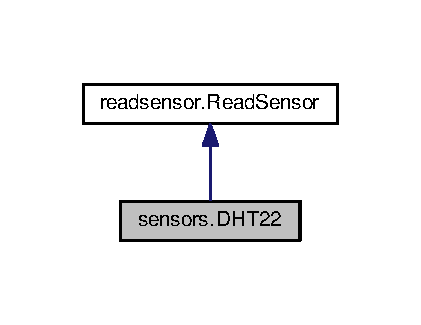
\includegraphics[width=202pt]{classsensors_1_1DHT22__inherit__graph}
\end{center}
\end{figure}


Collaboration diagram for sensors.\+D\+H\+T22\+:\nopagebreak
\begin{figure}[H]
\begin{center}
\leavevmode
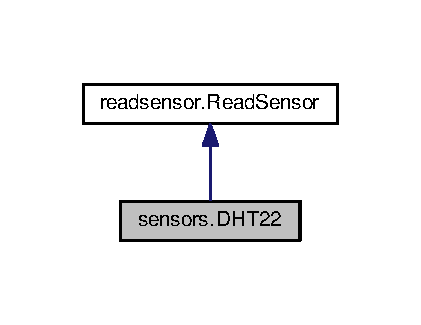
\includegraphics[width=202pt]{classsensors_1_1DHT22__coll__graph}
\end{center}
\end{figure}
\subsection*{Public Member Functions}
\begin{DoxyCompactItemize}
\item 
def \hyperlink{classsensors_1_1DHT22_a5958701fe5dfdaf901c03926ca5ffc33}{\+\_\+\+\_\+init\+\_\+\+\_\+} (self, prt, bdrate)
\item 
def \hyperlink{classsensors_1_1DHT22_a957aa77f0af01e9306aeb86d122969fc}{Interpret\+Response} (self)
\item 
def \hyperlink{classsensors_1_1DHT22_a5c20cdc8c8168efe52e9ce3ce0c3e819}{\+\_\+\+\_\+str\+\_\+\+\_\+} (self)
\end{DoxyCompactItemize}
\subsection*{Public Attributes}
\begin{DoxyCompactItemize}
\item 
\hyperlink{classsensors_1_1DHT22_a0f53e4181f2b2008ffe099a22631a617}{H}
\item 
\hyperlink{classsensors_1_1DHT22_a9055341fda2f3628ef888a39254d1c83}{unitH}
\item 
\hyperlink{classsensors_1_1DHT22_af42b72d6f11a320fe7e94a23734a109e}{T}
\item 
\hyperlink{classsensors_1_1DHT22_a9fab2812780c9f861d4bf8adc4d287d6}{unitT}
\item 
\hyperlink{classsensors_1_1DHT22_a1262c133aa610ada87b4ad2d508e8afd}{err}
\item 
\hyperlink{classsensors_1_1DHT22_a568f624009b01624445ef11fa20405f3}{cmd\+ID}
\item 
\hyperlink{classsensors_1_1DHT22_ab06cbe8e37c2eefe567c269c573eef80}{p\+String}
\item 
\hyperlink{classsensors_1_1DHT22_a77f4bf3d94cfee52d6ffb003800ae65b}{resp\+Mask}
\end{DoxyCompactItemize}


\subsection{Constructor \& Destructor Documentation}
\index{sensors\+::\+D\+H\+T22@{sensors\+::\+D\+H\+T22}!\+\_\+\+\_\+init\+\_\+\+\_\+@{\+\_\+\+\_\+init\+\_\+\+\_\+}}
\index{\+\_\+\+\_\+init\+\_\+\+\_\+@{\+\_\+\+\_\+init\+\_\+\+\_\+}!sensors\+::\+D\+H\+T22@{sensors\+::\+D\+H\+T22}}
\subsubsection[{\texorpdfstring{\+\_\+\+\_\+init\+\_\+\+\_\+(self, prt, bdrate)}{__init__(self, prt, bdrate)}}]{\setlength{\rightskip}{0pt plus 5cm}def sensors.\+D\+H\+T22.\+\_\+\+\_\+init\+\_\+\+\_\+ (
\begin{DoxyParamCaption}
\item[{}]{self, }
\item[{}]{prt, }
\item[{}]{bdrate}
\end{DoxyParamCaption}
)}\hypertarget{classsensors_1_1DHT22_a5958701fe5dfdaf901c03926ca5ffc33}{}\label{classsensors_1_1DHT22_a5958701fe5dfdaf901c03926ca5ffc33}


Here is the call graph for this function\+:\nopagebreak
\begin{figure}[H]
\begin{center}
\leavevmode
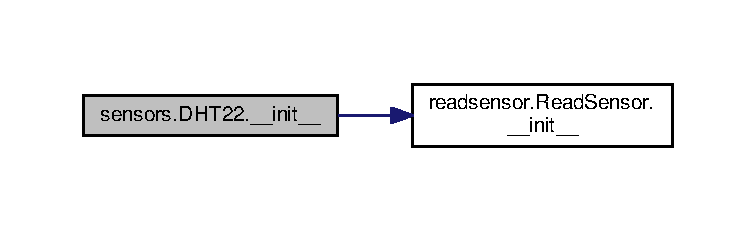
\includegraphics[width=350pt]{classsensors_1_1DHT22_a5958701fe5dfdaf901c03926ca5ffc33_cgraph}
\end{center}
\end{figure}




\subsection{Member Function Documentation}
\index{sensors\+::\+D\+H\+T22@{sensors\+::\+D\+H\+T22}!\+\_\+\+\_\+str\+\_\+\+\_\+@{\+\_\+\+\_\+str\+\_\+\+\_\+}}
\index{\+\_\+\+\_\+str\+\_\+\+\_\+@{\+\_\+\+\_\+str\+\_\+\+\_\+}!sensors\+::\+D\+H\+T22@{sensors\+::\+D\+H\+T22}}
\subsubsection[{\texorpdfstring{\+\_\+\+\_\+str\+\_\+\+\_\+(self)}{__str__(self)}}]{\setlength{\rightskip}{0pt plus 5cm}def sensors.\+D\+H\+T22.\+\_\+\+\_\+str\+\_\+\+\_\+ (
\begin{DoxyParamCaption}
\item[{}]{self}
\end{DoxyParamCaption}
)}\hypertarget{classsensors_1_1DHT22_a5c20cdc8c8168efe52e9ce3ce0c3e819}{}\label{classsensors_1_1DHT22_a5c20cdc8c8168efe52e9ce3ce0c3e819}
\index{sensors\+::\+D\+H\+T22@{sensors\+::\+D\+H\+T22}!Interpret\+Response@{Interpret\+Response}}
\index{Interpret\+Response@{Interpret\+Response}!sensors\+::\+D\+H\+T22@{sensors\+::\+D\+H\+T22}}
\subsubsection[{\texorpdfstring{Interpret\+Response(self)}{InterpretResponse(self)}}]{\setlength{\rightskip}{0pt plus 5cm}def sensors.\+D\+H\+T22.\+Interpret\+Response (
\begin{DoxyParamCaption}
\item[{}]{self}
\end{DoxyParamCaption}
)}\hypertarget{classsensors_1_1DHT22_a957aa77f0af01e9306aeb86d122969fc}{}\label{classsensors_1_1DHT22_a957aa77f0af01e9306aeb86d122969fc}
\begin{DoxyVerb}Interpret response list \end{DoxyVerb}
 

\subsection{Member Data Documentation}
\index{sensors\+::\+D\+H\+T22@{sensors\+::\+D\+H\+T22}!cmd\+ID@{cmd\+ID}}
\index{cmd\+ID@{cmd\+ID}!sensors\+::\+D\+H\+T22@{sensors\+::\+D\+H\+T22}}
\subsubsection[{\texorpdfstring{cmd\+ID}{cmdID}}]{\setlength{\rightskip}{0pt plus 5cm}sensors.\+D\+H\+T22.\+cmd\+ID}\hypertarget{classsensors_1_1DHT22_a568f624009b01624445ef11fa20405f3}{}\label{classsensors_1_1DHT22_a568f624009b01624445ef11fa20405f3}
\index{sensors\+::\+D\+H\+T22@{sensors\+::\+D\+H\+T22}!err@{err}}
\index{err@{err}!sensors\+::\+D\+H\+T22@{sensors\+::\+D\+H\+T22}}
\subsubsection[{\texorpdfstring{err}{err}}]{\setlength{\rightskip}{0pt plus 5cm}sensors.\+D\+H\+T22.\+err}\hypertarget{classsensors_1_1DHT22_a1262c133aa610ada87b4ad2d508e8afd}{}\label{classsensors_1_1DHT22_a1262c133aa610ada87b4ad2d508e8afd}
\index{sensors\+::\+D\+H\+T22@{sensors\+::\+D\+H\+T22}!H@{H}}
\index{H@{H}!sensors\+::\+D\+H\+T22@{sensors\+::\+D\+H\+T22}}
\subsubsection[{\texorpdfstring{H}{H}}]{\setlength{\rightskip}{0pt plus 5cm}sensors.\+D\+H\+T22.\+H}\hypertarget{classsensors_1_1DHT22_a0f53e4181f2b2008ffe099a22631a617}{}\label{classsensors_1_1DHT22_a0f53e4181f2b2008ffe099a22631a617}
\index{sensors\+::\+D\+H\+T22@{sensors\+::\+D\+H\+T22}!p\+String@{p\+String}}
\index{p\+String@{p\+String}!sensors\+::\+D\+H\+T22@{sensors\+::\+D\+H\+T22}}
\subsubsection[{\texorpdfstring{p\+String}{pString}}]{\setlength{\rightskip}{0pt plus 5cm}sensors.\+D\+H\+T22.\+p\+String}\hypertarget{classsensors_1_1DHT22_ab06cbe8e37c2eefe567c269c573eef80}{}\label{classsensors_1_1DHT22_ab06cbe8e37c2eefe567c269c573eef80}
\index{sensors\+::\+D\+H\+T22@{sensors\+::\+D\+H\+T22}!resp\+Mask@{resp\+Mask}}
\index{resp\+Mask@{resp\+Mask}!sensors\+::\+D\+H\+T22@{sensors\+::\+D\+H\+T22}}
\subsubsection[{\texorpdfstring{resp\+Mask}{respMask}}]{\setlength{\rightskip}{0pt plus 5cm}sensors.\+D\+H\+T22.\+resp\+Mask}\hypertarget{classsensors_1_1DHT22_a77f4bf3d94cfee52d6ffb003800ae65b}{}\label{classsensors_1_1DHT22_a77f4bf3d94cfee52d6ffb003800ae65b}
\index{sensors\+::\+D\+H\+T22@{sensors\+::\+D\+H\+T22}!T@{T}}
\index{T@{T}!sensors\+::\+D\+H\+T22@{sensors\+::\+D\+H\+T22}}
\subsubsection[{\texorpdfstring{T}{T}}]{\setlength{\rightskip}{0pt plus 5cm}sensors.\+D\+H\+T22.\+T}\hypertarget{classsensors_1_1DHT22_af42b72d6f11a320fe7e94a23734a109e}{}\label{classsensors_1_1DHT22_af42b72d6f11a320fe7e94a23734a109e}
\index{sensors\+::\+D\+H\+T22@{sensors\+::\+D\+H\+T22}!unitH@{unitH}}
\index{unitH@{unitH}!sensors\+::\+D\+H\+T22@{sensors\+::\+D\+H\+T22}}
\subsubsection[{\texorpdfstring{unitH}{unitH}}]{\setlength{\rightskip}{0pt plus 5cm}sensors.\+D\+H\+T22.\+unitH}\hypertarget{classsensors_1_1DHT22_a9055341fda2f3628ef888a39254d1c83}{}\label{classsensors_1_1DHT22_a9055341fda2f3628ef888a39254d1c83}
\index{sensors\+::\+D\+H\+T22@{sensors\+::\+D\+H\+T22}!unitT@{unitT}}
\index{unitT@{unitT}!sensors\+::\+D\+H\+T22@{sensors\+::\+D\+H\+T22}}
\subsubsection[{\texorpdfstring{unitT}{unitT}}]{\setlength{\rightskip}{0pt plus 5cm}sensors.\+D\+H\+T22.\+unitT}\hypertarget{classsensors_1_1DHT22_a9fab2812780c9f861d4bf8adc4d287d6}{}\label{classsensors_1_1DHT22_a9fab2812780c9f861d4bf8adc4d287d6}


The documentation for this class was generated from the following file\+:\begin{DoxyCompactItemize}
\item 
Python/\hyperlink{sensors_8py}{sensors.\+py}\end{DoxyCompactItemize}

\hypertarget{classsensors_1_1DS18B20}{}\section{sensors.\+D\+S18\+B20 Class Reference}
\label{classsensors_1_1DS18B20}\index{sensors.\+D\+S18\+B20@{sensors.\+D\+S18\+B20}}


Inheritance diagram for sensors.\+D\+S18\+B20\+:\nopagebreak
\begin{figure}[H]
\begin{center}
\leavevmode
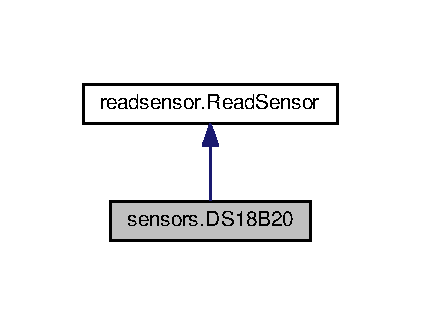
\includegraphics[width=202pt]{classsensors_1_1DS18B20__inherit__graph}
\end{center}
\end{figure}


Collaboration diagram for sensors.\+D\+S18\+B20\+:\nopagebreak
\begin{figure}[H]
\begin{center}
\leavevmode
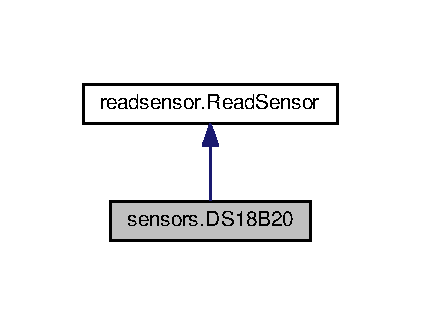
\includegraphics[width=202pt]{classsensors_1_1DS18B20__coll__graph}
\end{center}
\end{figure}
\subsection*{Public Member Functions}
\begin{DoxyCompactItemize}
\item 
def \hyperlink{classsensors_1_1DS18B20_a1029c5b384593c8b9d9826c4f8ba95dc}{\+\_\+\+\_\+init\+\_\+\+\_\+} (self, prt, bdrate)
\item 
def \hyperlink{classsensors_1_1DS18B20_a95d8a3d2b0e0e4ce4090a9d6778e189e}{Interpret\+Response} (self)
\item 
def \hyperlink{classsensors_1_1DS18B20_a00cce06ee0b0b920cb3df86cc5ad1902}{Get\+Value\+Pair} (self, idx)
\item 
def \hyperlink{classsensors_1_1DS18B20_abaf2d655c254d5595879e91860b545f8}{Get\+Avg\+Temperature} (self)
\item 
def \hyperlink{classsensors_1_1DS18B20_a88d7d94ab43332ceea56fa301de9c1d1}{\+\_\+\+\_\+str\+\_\+\+\_\+} (self)
\end{DoxyCompactItemize}
\subsection*{Public Attributes}
\begin{DoxyCompactItemize}
\item 
\hyperlink{classsensors_1_1DS18B20_a9b75c982811d488391ab52a339d58be8}{M\+AC}
\item 
\hyperlink{classsensors_1_1DS18B20_a738644d266b4149bdd79e1a269e555ad}{T}
\item 
\hyperlink{classsensors_1_1DS18B20_a2a93fcbbf67debf4356c6c3a9b2b58f3}{unitT}
\item 
\hyperlink{classsensors_1_1DS18B20_a8d25c7e23f6b3e1b424dac9209538a53}{node\+M\+AC}
\item 
\hyperlink{classsensors_1_1DS18B20_a8a7911c0b96b5c78d097254187f323cc}{cmd\+ID}
\item 
\hyperlink{classsensors_1_1DS18B20_a9edc6c09ffba98f42e5b7cad1685d564}{p\+String}
\item 
\hyperlink{classsensors_1_1DS18B20_ac064c221c0d23deb28ec74e3e9bb6510}{resp\+Mask}
\item 
\hyperlink{classsensors_1_1DS18B20_aef41d6169e461effa962dc97ade7e9ad}{num\+El}
\end{DoxyCompactItemize}


\subsection{Constructor \& Destructor Documentation}
\index{sensors\+::\+D\+S18\+B20@{sensors\+::\+D\+S18\+B20}!\+\_\+\+\_\+init\+\_\+\+\_\+@{\+\_\+\+\_\+init\+\_\+\+\_\+}}
\index{\+\_\+\+\_\+init\+\_\+\+\_\+@{\+\_\+\+\_\+init\+\_\+\+\_\+}!sensors\+::\+D\+S18\+B20@{sensors\+::\+D\+S18\+B20}}
\subsubsection[{\texorpdfstring{\+\_\+\+\_\+init\+\_\+\+\_\+(self, prt, bdrate)}{__init__(self, prt, bdrate)}}]{\setlength{\rightskip}{0pt plus 5cm}def sensors.\+D\+S18\+B20.\+\_\+\+\_\+init\+\_\+\+\_\+ (
\begin{DoxyParamCaption}
\item[{}]{self, }
\item[{}]{prt, }
\item[{}]{bdrate}
\end{DoxyParamCaption}
)}\hypertarget{classsensors_1_1DS18B20_a1029c5b384593c8b9d9826c4f8ba95dc}{}\label{classsensors_1_1DS18B20_a1029c5b384593c8b9d9826c4f8ba95dc}


Here is the call graph for this function\+:\nopagebreak
\begin{figure}[H]
\begin{center}
\leavevmode
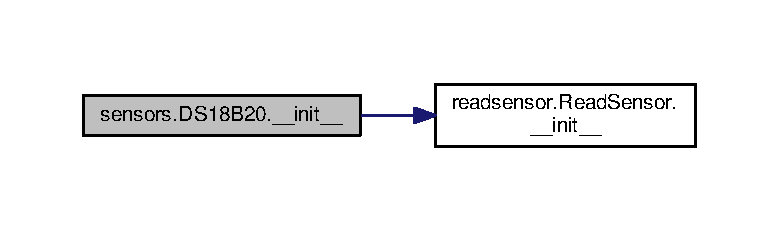
\includegraphics[width=350pt]{classsensors_1_1DS18B20_a1029c5b384593c8b9d9826c4f8ba95dc_cgraph}
\end{center}
\end{figure}




\subsection{Member Function Documentation}
\index{sensors\+::\+D\+S18\+B20@{sensors\+::\+D\+S18\+B20}!\+\_\+\+\_\+str\+\_\+\+\_\+@{\+\_\+\+\_\+str\+\_\+\+\_\+}}
\index{\+\_\+\+\_\+str\+\_\+\+\_\+@{\+\_\+\+\_\+str\+\_\+\+\_\+}!sensors\+::\+D\+S18\+B20@{sensors\+::\+D\+S18\+B20}}
\subsubsection[{\texorpdfstring{\+\_\+\+\_\+str\+\_\+\+\_\+(self)}{__str__(self)}}]{\setlength{\rightskip}{0pt plus 5cm}def sensors.\+D\+S18\+B20.\+\_\+\+\_\+str\+\_\+\+\_\+ (
\begin{DoxyParamCaption}
\item[{}]{self}
\end{DoxyParamCaption}
)}\hypertarget{classsensors_1_1DS18B20_a88d7d94ab43332ceea56fa301de9c1d1}{}\label{classsensors_1_1DS18B20_a88d7d94ab43332ceea56fa301de9c1d1}


Here is the call graph for this function\+:\nopagebreak
\begin{figure}[H]
\begin{center}
\leavevmode
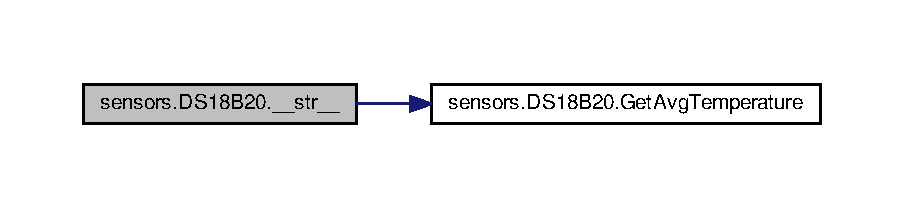
\includegraphics[width=350pt]{classsensors_1_1DS18B20_a88d7d94ab43332ceea56fa301de9c1d1_cgraph}
\end{center}
\end{figure}


\index{sensors\+::\+D\+S18\+B20@{sensors\+::\+D\+S18\+B20}!Get\+Avg\+Temperature@{Get\+Avg\+Temperature}}
\index{Get\+Avg\+Temperature@{Get\+Avg\+Temperature}!sensors\+::\+D\+S18\+B20@{sensors\+::\+D\+S18\+B20}}
\subsubsection[{\texorpdfstring{Get\+Avg\+Temperature(self)}{GetAvgTemperature(self)}}]{\setlength{\rightskip}{0pt plus 5cm}def sensors.\+D\+S18\+B20.\+Get\+Avg\+Temperature (
\begin{DoxyParamCaption}
\item[{}]{self}
\end{DoxyParamCaption}
)}\hypertarget{classsensors_1_1DS18B20_abaf2d655c254d5595879e91860b545f8}{}\label{classsensors_1_1DS18B20_abaf2d655c254d5595879e91860b545f8}
\index{sensors\+::\+D\+S18\+B20@{sensors\+::\+D\+S18\+B20}!Get\+Value\+Pair@{Get\+Value\+Pair}}
\index{Get\+Value\+Pair@{Get\+Value\+Pair}!sensors\+::\+D\+S18\+B20@{sensors\+::\+D\+S18\+B20}}
\subsubsection[{\texorpdfstring{Get\+Value\+Pair(self, idx)}{GetValuePair(self, idx)}}]{\setlength{\rightskip}{0pt plus 5cm}def sensors.\+D\+S18\+B20.\+Get\+Value\+Pair (
\begin{DoxyParamCaption}
\item[{}]{self, }
\item[{}]{idx}
\end{DoxyParamCaption}
)}\hypertarget{classsensors_1_1DS18B20_a00cce06ee0b0b920cb3df86cc5ad1902}{}\label{classsensors_1_1DS18B20_a00cce06ee0b0b920cb3df86cc5ad1902}
\index{sensors\+::\+D\+S18\+B20@{sensors\+::\+D\+S18\+B20}!Interpret\+Response@{Interpret\+Response}}
\index{Interpret\+Response@{Interpret\+Response}!sensors\+::\+D\+S18\+B20@{sensors\+::\+D\+S18\+B20}}
\subsubsection[{\texorpdfstring{Interpret\+Response(self)}{InterpretResponse(self)}}]{\setlength{\rightskip}{0pt plus 5cm}def sensors.\+D\+S18\+B20.\+Interpret\+Response (
\begin{DoxyParamCaption}
\item[{}]{self}
\end{DoxyParamCaption}
)}\hypertarget{classsensors_1_1DS18B20_a95d8a3d2b0e0e4ce4090a9d6778e189e}{}\label{classsensors_1_1DS18B20_a95d8a3d2b0e0e4ce4090a9d6778e189e}
\begin{DoxyVerb}Interpret response list \end{DoxyVerb}
 

\subsection{Member Data Documentation}
\index{sensors\+::\+D\+S18\+B20@{sensors\+::\+D\+S18\+B20}!cmd\+ID@{cmd\+ID}}
\index{cmd\+ID@{cmd\+ID}!sensors\+::\+D\+S18\+B20@{sensors\+::\+D\+S18\+B20}}
\subsubsection[{\texorpdfstring{cmd\+ID}{cmdID}}]{\setlength{\rightskip}{0pt plus 5cm}sensors.\+D\+S18\+B20.\+cmd\+ID}\hypertarget{classsensors_1_1DS18B20_a8a7911c0b96b5c78d097254187f323cc}{}\label{classsensors_1_1DS18B20_a8a7911c0b96b5c78d097254187f323cc}
\index{sensors\+::\+D\+S18\+B20@{sensors\+::\+D\+S18\+B20}!M\+AC@{M\+AC}}
\index{M\+AC@{M\+AC}!sensors\+::\+D\+S18\+B20@{sensors\+::\+D\+S18\+B20}}
\subsubsection[{\texorpdfstring{M\+AC}{MAC}}]{\setlength{\rightskip}{0pt plus 5cm}sensors.\+D\+S18\+B20.\+M\+AC}\hypertarget{classsensors_1_1DS18B20_a9b75c982811d488391ab52a339d58be8}{}\label{classsensors_1_1DS18B20_a9b75c982811d488391ab52a339d58be8}
\index{sensors\+::\+D\+S18\+B20@{sensors\+::\+D\+S18\+B20}!node\+M\+AC@{node\+M\+AC}}
\index{node\+M\+AC@{node\+M\+AC}!sensors\+::\+D\+S18\+B20@{sensors\+::\+D\+S18\+B20}}
\subsubsection[{\texorpdfstring{node\+M\+AC}{nodeMAC}}]{\setlength{\rightskip}{0pt plus 5cm}sensors.\+D\+S18\+B20.\+node\+M\+AC}\hypertarget{classsensors_1_1DS18B20_a8d25c7e23f6b3e1b424dac9209538a53}{}\label{classsensors_1_1DS18B20_a8d25c7e23f6b3e1b424dac9209538a53}
\index{sensors\+::\+D\+S18\+B20@{sensors\+::\+D\+S18\+B20}!num\+El@{num\+El}}
\index{num\+El@{num\+El}!sensors\+::\+D\+S18\+B20@{sensors\+::\+D\+S18\+B20}}
\subsubsection[{\texorpdfstring{num\+El}{numEl}}]{\setlength{\rightskip}{0pt plus 5cm}sensors.\+D\+S18\+B20.\+num\+El}\hypertarget{classsensors_1_1DS18B20_aef41d6169e461effa962dc97ade7e9ad}{}\label{classsensors_1_1DS18B20_aef41d6169e461effa962dc97ade7e9ad}
\index{sensors\+::\+D\+S18\+B20@{sensors\+::\+D\+S18\+B20}!p\+String@{p\+String}}
\index{p\+String@{p\+String}!sensors\+::\+D\+S18\+B20@{sensors\+::\+D\+S18\+B20}}
\subsubsection[{\texorpdfstring{p\+String}{pString}}]{\setlength{\rightskip}{0pt plus 5cm}sensors.\+D\+S18\+B20.\+p\+String}\hypertarget{classsensors_1_1DS18B20_a9edc6c09ffba98f42e5b7cad1685d564}{}\label{classsensors_1_1DS18B20_a9edc6c09ffba98f42e5b7cad1685d564}
\index{sensors\+::\+D\+S18\+B20@{sensors\+::\+D\+S18\+B20}!resp\+Mask@{resp\+Mask}}
\index{resp\+Mask@{resp\+Mask}!sensors\+::\+D\+S18\+B20@{sensors\+::\+D\+S18\+B20}}
\subsubsection[{\texorpdfstring{resp\+Mask}{respMask}}]{\setlength{\rightskip}{0pt plus 5cm}sensors.\+D\+S18\+B20.\+resp\+Mask}\hypertarget{classsensors_1_1DS18B20_ac064c221c0d23deb28ec74e3e9bb6510}{}\label{classsensors_1_1DS18B20_ac064c221c0d23deb28ec74e3e9bb6510}
\index{sensors\+::\+D\+S18\+B20@{sensors\+::\+D\+S18\+B20}!T@{T}}
\index{T@{T}!sensors\+::\+D\+S18\+B20@{sensors\+::\+D\+S18\+B20}}
\subsubsection[{\texorpdfstring{T}{T}}]{\setlength{\rightskip}{0pt plus 5cm}sensors.\+D\+S18\+B20.\+T}\hypertarget{classsensors_1_1DS18B20_a738644d266b4149bdd79e1a269e555ad}{}\label{classsensors_1_1DS18B20_a738644d266b4149bdd79e1a269e555ad}
\index{sensors\+::\+D\+S18\+B20@{sensors\+::\+D\+S18\+B20}!unitT@{unitT}}
\index{unitT@{unitT}!sensors\+::\+D\+S18\+B20@{sensors\+::\+D\+S18\+B20}}
\subsubsection[{\texorpdfstring{unitT}{unitT}}]{\setlength{\rightskip}{0pt plus 5cm}sensors.\+D\+S18\+B20.\+unitT}\hypertarget{classsensors_1_1DS18B20_a2a93fcbbf67debf4356c6c3a9b2b58f3}{}\label{classsensors_1_1DS18B20_a2a93fcbbf67debf4356c6c3a9b2b58f3}


The documentation for this class was generated from the following file\+:\begin{DoxyCompactItemize}
\item 
Python/\hyperlink{sensors_8py}{sensors.\+py}\end{DoxyCompactItemize}

\hypertarget{classDS18B20}{}\section{D\+S18\+B20 Class Reference}
\label{classDS18B20}\index{D\+S18\+B20@{D\+S18\+B20}}


\hyperlink{classDS18B20}{D\+S18\+B20} class definition.  




{\ttfamily \#include $<$D\+S18\+B20.\+h$>$}

\subsection*{Public Member Functions}
\begin{DoxyCompactItemize}
\item 
void \hyperlink{classDS18B20_a6340d31cea87cf473af13fc7f15f60e4}{Read\+Measurement} (char $\ast$string)
\begin{DoxyCompactList}\small\item\em Takes a Measurement per sensor on the bus. \end{DoxyCompactList}\item 
void \hyperlink{classDS18B20_a440a17340ac61a693316550422e4ae4e}{Read\+Measurement2} (char $\ast$Macstring, char $\ast$temp\+Str)
\begin{DoxyCompactList}\small\item\em Takes a Measurement per sensor on the bus. \end{DoxyCompactList}\item 
\hyperlink{classDS18B20_afc1a4166a4d1d00baef15a9e4c59b632}{D\+S18\+B20} ()
\begin{DoxyCompactList}\small\item\em \hyperlink{classDS18B20}{D\+S18\+B20} standard constructor. \end{DoxyCompactList}\item 
\hyperlink{classDS18B20_afb0ce114e04bc699bc2e3c5282a31bc3}{D\+S18\+B20} (volatile uint8\+\_\+t \&Wire\+\_\+\+P\+O\+RT, volatile uint8\+\_\+t \&Wire\+\_\+\+D\+DR, volatile uint8\+\_\+t \&Wire\+\_\+\+P\+IN, uint8\+\_\+t Wire\+\_\+\+DQ)
\begin{DoxyCompactList}\small\item\em \hyperlink{classDS18B20}{D\+S18\+B20} constructor. \end{DoxyCompactList}\item 
void \hyperlink{classDS18B20_af18146fd823d04f5472fb305e46f02b0}{Get\+M\+A\+C\+String} (char $\ast$M\+A\+C\+String\+Out)
\begin{DoxyCompactList}\small\item\em Get M\+AC addresses from M\+A\+C\+String. \end{DoxyCompactList}\item 
void \hyperlink{classDS18B20_a64a03b4a18a9d2b3faeb7943865055e9}{Get\+Sensor\+String\+X\+ML} (char $\ast$string)
\begin{DoxyCompactList}\small\item\em Get xml style sensor string. \end{DoxyCompactList}\item 
void \hyperlink{classDS18B20_ae3d50f1b5b71517d633958f54654ea55}{Get\+Temperature} (char $\ast$M\+A\+Cstring, char $\ast$temp\+String)
\begin{DoxyCompactList}\small\item\em Get temperature values in one string an the M\+AC addresses in a seperate one. \end{DoxyCompactList}\end{DoxyCompactItemize}
\subsection*{Private Member Functions}
\begin{DoxyCompactItemize}
\item 
void \hyperlink{classDS18B20_a817183f6ef9552d6559d58d714e5c804}{Start\+Measurement} (void)
\item 
uint8\+\_\+t \hyperlink{classDS18B20_a890b94747fbd3ec6e45088735c7bc1fe}{Reset} ()
\item 
uint8\+\_\+t \hyperlink{classDS18B20_ac2bf79674d18e4ad00d7b41d76d411e3}{Bit\+IO} (uint8\+\_\+t bit)
\item 
uint8\+\_\+t \hyperlink{classDS18B20_a7314cb6a438ddd0c214ed409f7dd5d86}{Write\+Byte} (uint8\+\_\+t byte)
\item 
uint8\+\_\+t \hyperlink{classDS18B20_aa43d0c42ebb25bbdc9b7904710652c75}{Read\+Byte} (void)
\item 
unsigned char \hyperlink{classDS18B20_a356e88e8a6bca4f5ffeb41180c08f91d}{Rom\+Search} (unsigned char diff, unsigned char $\ast$id)
\item 
void \hyperlink{classDS18B20_a1f03dae7ea2d07a225343eaa33d119cf}{Command} (unsigned char command, unsigned char $\ast$id)
\item 
void \hyperlink{classDS18B20_abd68014bd97396c4b0365d3e1ca1f61c}{P\+I\+N\+\_\+\+I\+N\+P\+U\+T\+\_\+\+M\+O\+DE} ()
\item 
void \hyperlink{classDS18B20_aaa611dcdffd8f02719f62c8a93c0c7c0}{P\+I\+N\+\_\+\+O\+U\+T\+P\+U\+T\+\_\+\+M\+O\+DE} ()
\item 
void \hyperlink{classDS18B20_a8a8a45bbfe229978ea7280177b6fe18b}{P\+I\+N\+\_\+\+L\+OW} ()
\item 
void \hyperlink{classDS18B20_af9d029958b4a835a15867df7ad59d7d3}{P\+I\+N\+\_\+\+H\+I\+GH} ()
\item 
\hyperlink{classDS18B20_a458a891af1a3631958fa84c5b5bbc457}{\+\_\+\+\_\+attribute\+\_\+\+\_\+} ((gnu\+\_\+inline)) void delay\+\_\+us(uint16\+\_\+t delay)
\end{DoxyCompactItemize}
\subsection*{Private Attributes}
\begin{DoxyCompactItemize}
\item 
volatile uint8\+\_\+t $\ast$ \hyperlink{classDS18B20_a4e8d420cd118999883bde12e766bc1d4}{W\+I\+R\+E\+\_\+\+P\+O\+RT}
\begin{DoxyCompactList}\small\item\em Thermometer data port. \end{DoxyCompactList}\item 
volatile uint8\+\_\+t $\ast$ \hyperlink{classDS18B20_a06a1f548d087b8d8971dee5e94653f5c}{W\+I\+R\+E\+\_\+\+D\+DR}
\begin{DoxyCompactList}\small\item\em Thermometer data port. \end{DoxyCompactList}\item 
volatile uint8\+\_\+t $\ast$ \hyperlink{classDS18B20_a03a1ad890f9713fc10dc353c9779a7f2}{W\+I\+R\+E\+\_\+\+P\+IN}
\begin{DoxyCompactList}\small\item\em Thermometer data port. \end{DoxyCompactList}\item 
uint8\+\_\+t \hyperlink{classDS18B20_aebc6a6ab3c604f19dac9a24ef3301938}{W\+I\+R\+E\+\_\+\+DQ}
\begin{DoxyCompactList}\small\item\em Thermometer data line. \end{DoxyCompactList}\item 
char \hyperlink{classDS18B20_a6884de10b175289718239bdac0b8e52e}{M\+A\+C\+String} \mbox{[}120\mbox{]}
\begin{DoxyCompactList}\small\item\em M\+AC string of the sensor. \end{DoxyCompactList}\end{DoxyCompactItemize}


\subsection{Detailed Description}
\hyperlink{classDS18B20}{D\+S18\+B20} class definition. 

Defines methods for accessing the \hyperlink{classDS18B20}{D\+S18\+B20} interface 

\subsection{Constructor \& Destructor Documentation}
\index{D\+S18\+B20@{D\+S18\+B20}!D\+S18\+B20@{D\+S18\+B20}}
\index{D\+S18\+B20@{D\+S18\+B20}!D\+S18\+B20@{D\+S18\+B20}}
\subsubsection[{\texorpdfstring{D\+S18\+B20()}{DS18B20()}}]{\setlength{\rightskip}{0pt plus 5cm}D\+S18\+B20\+::\+D\+S18\+B20 (
\begin{DoxyParamCaption}
{}
\end{DoxyParamCaption}
)}\hypertarget{classDS18B20_afc1a4166a4d1d00baef15a9e4c59b632}{}\label{classDS18B20_afc1a4166a4d1d00baef15a9e4c59b632}


\hyperlink{classDS18B20}{D\+S18\+B20} standard constructor. 

new \hyperlink{classDS18B20}{D\+S18\+B20} object and initializes variables \index{D\+S18\+B20@{D\+S18\+B20}!D\+S18\+B20@{D\+S18\+B20}}
\index{D\+S18\+B20@{D\+S18\+B20}!D\+S18\+B20@{D\+S18\+B20}}
\subsubsection[{\texorpdfstring{D\+S18\+B20(volatile uint8\+\_\+t \&\+Wire\+\_\+\+P\+O\+R\+T, volatile uint8\+\_\+t \&\+Wire\+\_\+\+D\+D\+R, volatile uint8\+\_\+t \&\+Wire\+\_\+\+P\+I\+N, uint8\+\_\+t Wire\+\_\+\+D\+Q)}{DS18B20(volatile uint8_t &Wire_PORT, volatile uint8_t &Wire_DDR, volatile uint8_t &Wire_PIN, uint8_t Wire_DQ)}}]{\setlength{\rightskip}{0pt plus 5cm}D\+S18\+B20\+::\+D\+S18\+B20 (
\begin{DoxyParamCaption}
\item[{volatile uint8\+\_\+t \&}]{Wire\+\_\+\+P\+O\+RT, }
\item[{volatile uint8\+\_\+t \&}]{Wire\+\_\+\+D\+DR, }
\item[{volatile uint8\+\_\+t \&}]{Wire\+\_\+\+P\+IN, }
\item[{uint8\+\_\+t}]{Wire\+\_\+\+DQ}
\end{DoxyParamCaption}
)}\hypertarget{classDS18B20_afb0ce114e04bc699bc2e3c5282a31bc3}{}\label{classDS18B20_afb0ce114e04bc699bc2e3c5282a31bc3}


\hyperlink{classDS18B20}{D\+S18\+B20} constructor. 


\begin{DoxyParams}[1]{Parameters}
\mbox{\tt in}  & {\em Wire\+\_\+\+P\+O\+RT} & \\
\hline
\mbox{\tt in}  & {\em Wire\+\_\+\+D\+DR} & \\
\hline
\mbox{\tt in}  & {\em Wire\+\_\+\+P\+IN} & \\
\hline
\mbox{\tt in}  & {\em Wire\+\_\+\+DQ} & Data line \\
\hline
\end{DoxyParams}


\subsection{Member Function Documentation}
\index{D\+S18\+B20@{D\+S18\+B20}!\+\_\+\+\_\+attribute\+\_\+\+\_\+@{\+\_\+\+\_\+attribute\+\_\+\+\_\+}}
\index{\+\_\+\+\_\+attribute\+\_\+\+\_\+@{\+\_\+\+\_\+attribute\+\_\+\+\_\+}!D\+S18\+B20@{D\+S18\+B20}}
\subsubsection[{\texorpdfstring{\+\_\+\+\_\+attribute\+\_\+\+\_\+((gnu\+\_\+inline)) void delay\+\_\+us(uint16\+\_\+t delay)}{__attribute__((gnu_inline)) void delay_us(uint16_t delay)}}]{\setlength{\rightskip}{0pt plus 5cm}D\+S18\+B20\+::\+\_\+\+\_\+attribute\+\_\+\+\_\+ (
\begin{DoxyParamCaption}
\item[{(gnu\+\_\+inline)}]{}
\end{DoxyParamCaption}
)\hspace{0.3cm}{\ttfamily [inline]}, {\ttfamily [private]}}\hypertarget{classDS18B20_a458a891af1a3631958fa84c5b5bbc457}{}\label{classDS18B20_a458a891af1a3631958fa84c5b5bbc457}
\index{D\+S18\+B20@{D\+S18\+B20}!Bit\+IO@{Bit\+IO}}
\index{Bit\+IO@{Bit\+IO}!D\+S18\+B20@{D\+S18\+B20}}
\subsubsection[{\texorpdfstring{Bit\+I\+O(uint8\+\_\+t bit)}{BitIO(uint8_t bit)}}]{\setlength{\rightskip}{0pt plus 5cm}uint8\+\_\+t D\+S18\+B20\+::\+Bit\+IO (
\begin{DoxyParamCaption}
\item[{uint8\+\_\+t}]{bit}
\end{DoxyParamCaption}
)\hspace{0.3cm}{\ttfamily [private]}}\hypertarget{classDS18B20_ac2bf79674d18e4ad00d7b41d76d411e3}{}\label{classDS18B20_ac2bf79674d18e4ad00d7b41d76d411e3}


Here is the call graph for this function\+:\nopagebreak
\begin{figure}[H]
\begin{center}
\leavevmode
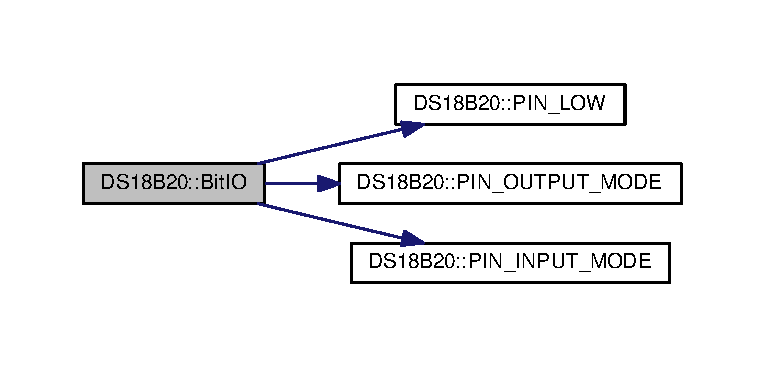
\includegraphics[width=350pt]{classDS18B20_ac2bf79674d18e4ad00d7b41d76d411e3_cgraph}
\end{center}
\end{figure}


\index{D\+S18\+B20@{D\+S18\+B20}!Command@{Command}}
\index{Command@{Command}!D\+S18\+B20@{D\+S18\+B20}}
\subsubsection[{\texorpdfstring{Command(unsigned char command, unsigned char $\ast$id)}{Command(unsigned char command, unsigned char *id)}}]{\setlength{\rightskip}{0pt plus 5cm}void D\+S18\+B20\+::\+Command (
\begin{DoxyParamCaption}
\item[{unsigned char}]{command, }
\item[{unsigned char $\ast$}]{id}
\end{DoxyParamCaption}
)\hspace{0.3cm}{\ttfamily [private]}}\hypertarget{classDS18B20_a1f03dae7ea2d07a225343eaa33d119cf}{}\label{classDS18B20_a1f03dae7ea2d07a225343eaa33d119cf}


Here is the call graph for this function\+:\nopagebreak
\begin{figure}[H]
\begin{center}
\leavevmode
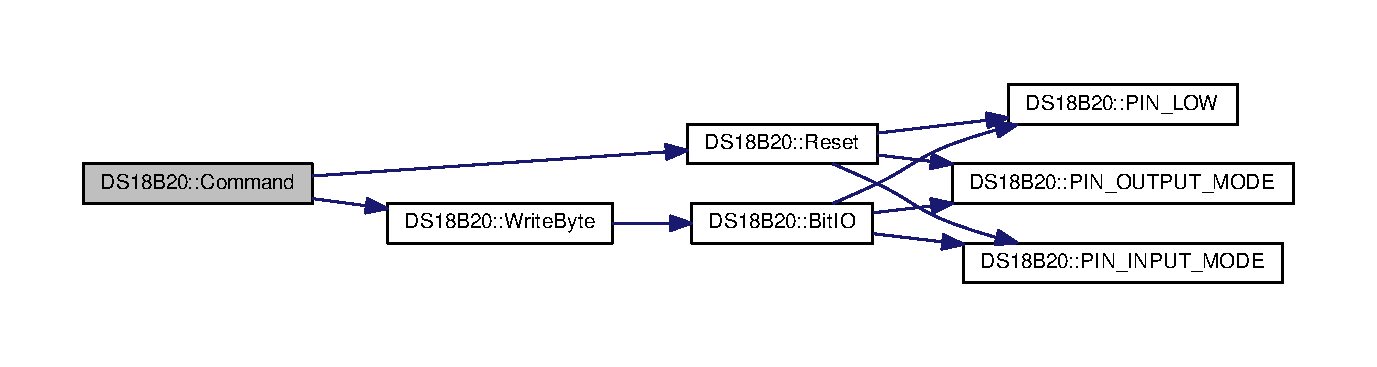
\includegraphics[width=350pt]{classDS18B20_a1f03dae7ea2d07a225343eaa33d119cf_cgraph}
\end{center}
\end{figure}


\index{D\+S18\+B20@{D\+S18\+B20}!Get\+M\+A\+C\+String@{Get\+M\+A\+C\+String}}
\index{Get\+M\+A\+C\+String@{Get\+M\+A\+C\+String}!D\+S18\+B20@{D\+S18\+B20}}
\subsubsection[{\texorpdfstring{Get\+M\+A\+C\+String(char $\ast$\+M\+A\+C\+String\+Out)}{GetMACString(char *MACStringOut)}}]{\setlength{\rightskip}{0pt plus 5cm}void D\+S18\+B20\+::\+Get\+M\+A\+C\+String (
\begin{DoxyParamCaption}
\item[{char $\ast$}]{M\+A\+C\+String\+Out}
\end{DoxyParamCaption}
)}\hypertarget{classDS18B20_af18146fd823d04f5472fb305e46f02b0}{}\label{classDS18B20_af18146fd823d04f5472fb305e46f02b0}


Get M\+AC addresses from M\+A\+C\+String. 


\begin{DoxyParams}[1]{Parameters}
\mbox{\tt out}  & {\em M\+A\+C\+String\+Out} & Character array of M\+AC addresses \\
\hline
\end{DoxyParams}
\index{D\+S18\+B20@{D\+S18\+B20}!Get\+Sensor\+String\+X\+ML@{Get\+Sensor\+String\+X\+ML}}
\index{Get\+Sensor\+String\+X\+ML@{Get\+Sensor\+String\+X\+ML}!D\+S18\+B20@{D\+S18\+B20}}
\subsubsection[{\texorpdfstring{Get\+Sensor\+String\+X\+M\+L(char $\ast$string)}{GetSensorStringXML(char *string)}}]{\setlength{\rightskip}{0pt plus 5cm}void D\+S18\+B20\+::\+Get\+Sensor\+String\+X\+ML (
\begin{DoxyParamCaption}
\item[{char $\ast$}]{string}
\end{DoxyParamCaption}
)}\hypertarget{classDS18B20_a64a03b4a18a9d2b3faeb7943865055e9}{}\label{classDS18B20_a64a03b4a18a9d2b3faeb7943865055e9}


Get xml style sensor string. 

Puts out one string with M\+AC addresses and their temperature values 
\begin{DoxyParams}[1]{Parameters}
\mbox{\tt out}  & {\em string} & X\+ML style sensor string \\
\hline
\end{DoxyParams}


Here is the call graph for this function\+:
\nopagebreak
\begin{figure}[H]
\begin{center}
\leavevmode
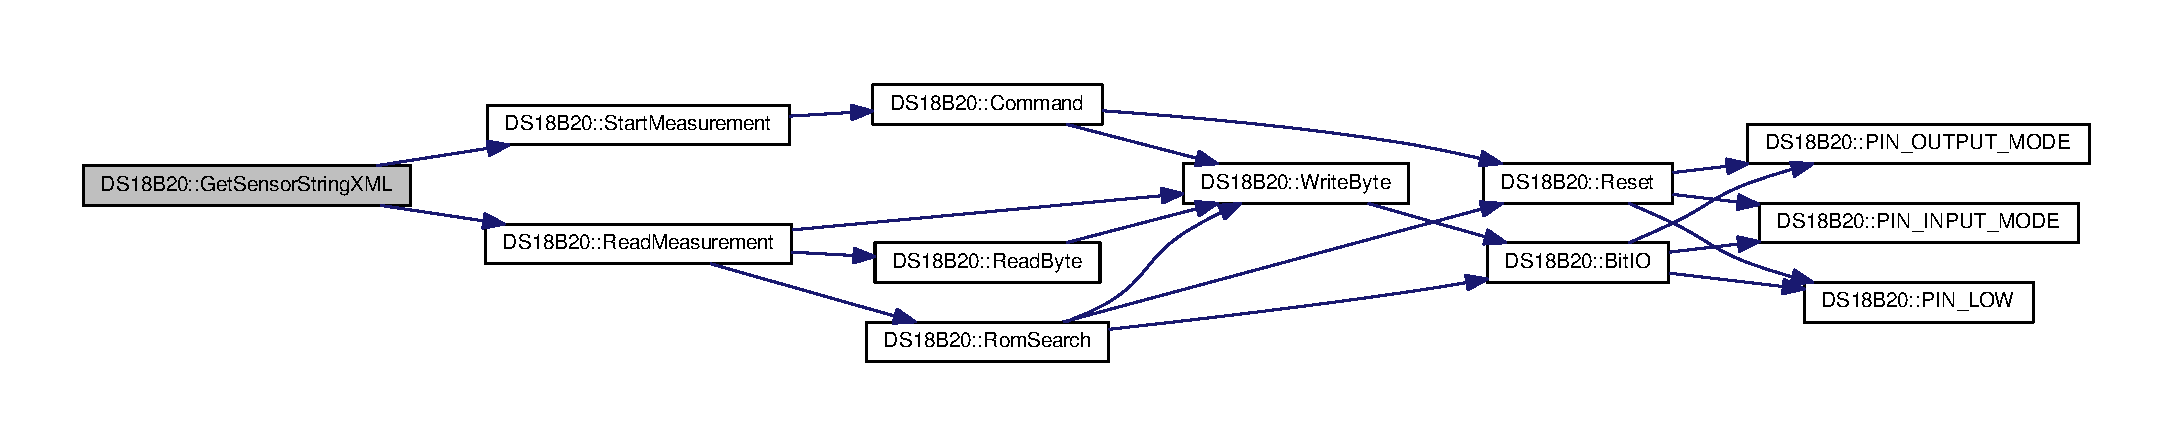
\includegraphics[width=350pt]{classDS18B20_a64a03b4a18a9d2b3faeb7943865055e9_cgraph}
\end{center}
\end{figure}


\index{D\+S18\+B20@{D\+S18\+B20}!Get\+Temperature@{Get\+Temperature}}
\index{Get\+Temperature@{Get\+Temperature}!D\+S18\+B20@{D\+S18\+B20}}
\subsubsection[{\texorpdfstring{Get\+Temperature(char $\ast$\+M\+A\+Cstring, char $\ast$temp\+String)}{GetTemperature(char *MACstring, char *tempString)}}]{\setlength{\rightskip}{0pt plus 5cm}void D\+S18\+B20\+::\+Get\+Temperature (
\begin{DoxyParamCaption}
\item[{char $\ast$}]{M\+A\+Cstring, }
\item[{char $\ast$}]{temp\+String}
\end{DoxyParamCaption}
)}\hypertarget{classDS18B20_ae3d50f1b5b71517d633958f54654ea55}{}\label{classDS18B20_ae3d50f1b5b71517d633958f54654ea55}


Get temperature values in one string an the M\+AC addresses in a seperate one. 


\begin{DoxyParams}[1]{Parameters}
\mbox{\tt out}  & {\em M\+A\+Cstring} & M\+AC addresses of each sensor on the bus \\
\hline
\mbox{\tt out}  & {\em temp\+String} & Temperature values in one string \\
\hline
\end{DoxyParams}


Here is the call graph for this function\+:
\nopagebreak
\begin{figure}[H]
\begin{center}
\leavevmode
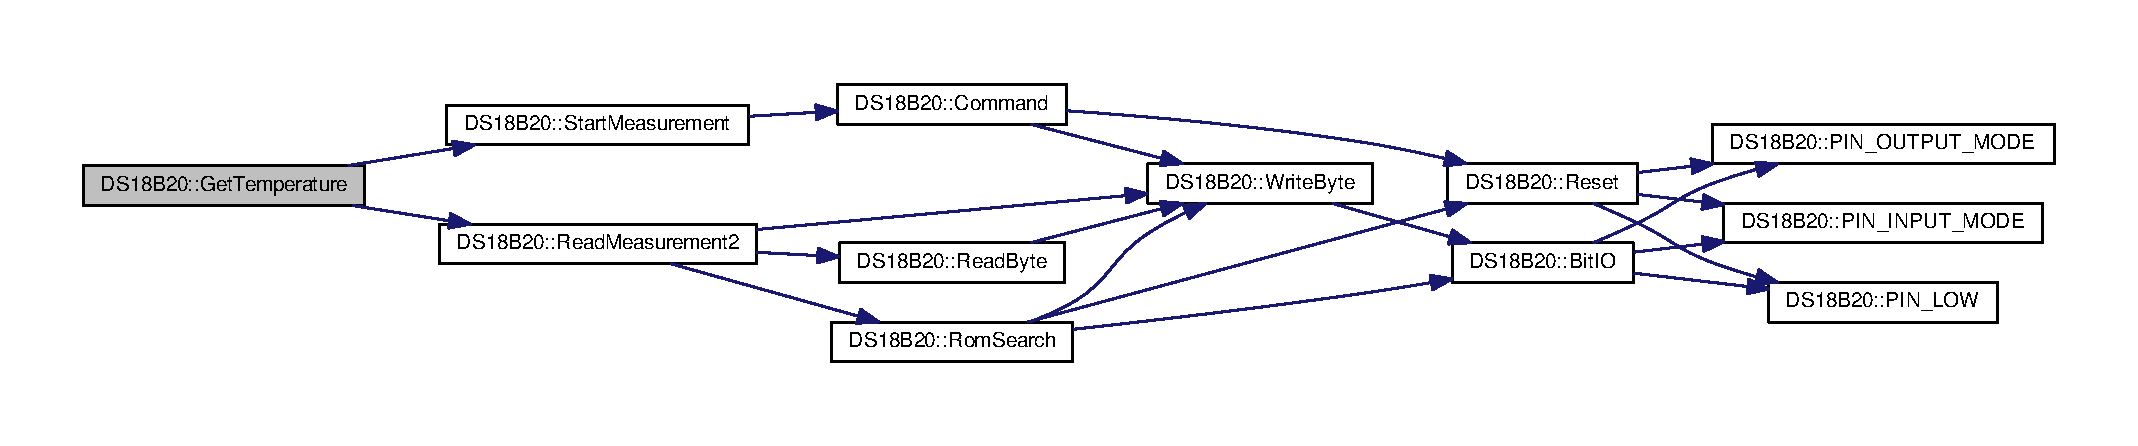
\includegraphics[width=350pt]{classDS18B20_ae3d50f1b5b71517d633958f54654ea55_cgraph}
\end{center}
\end{figure}


\index{D\+S18\+B20@{D\+S18\+B20}!P\+I\+N\+\_\+\+H\+I\+GH@{P\+I\+N\+\_\+\+H\+I\+GH}}
\index{P\+I\+N\+\_\+\+H\+I\+GH@{P\+I\+N\+\_\+\+H\+I\+GH}!D\+S18\+B20@{D\+S18\+B20}}
\subsubsection[{\texorpdfstring{P\+I\+N\+\_\+\+H\+I\+G\+H()}{PIN_HIGH()}}]{\setlength{\rightskip}{0pt plus 5cm}void D\+S18\+B20\+::\+P\+I\+N\+\_\+\+H\+I\+GH (
\begin{DoxyParamCaption}
{}
\end{DoxyParamCaption}
)\hspace{0.3cm}{\ttfamily [inline]}, {\ttfamily [private]}}\hypertarget{classDS18B20_af9d029958b4a835a15867df7ad59d7d3}{}\label{classDS18B20_af9d029958b4a835a15867df7ad59d7d3}
\index{D\+S18\+B20@{D\+S18\+B20}!P\+I\+N\+\_\+\+I\+N\+P\+U\+T\+\_\+\+M\+O\+DE@{P\+I\+N\+\_\+\+I\+N\+P\+U\+T\+\_\+\+M\+O\+DE}}
\index{P\+I\+N\+\_\+\+I\+N\+P\+U\+T\+\_\+\+M\+O\+DE@{P\+I\+N\+\_\+\+I\+N\+P\+U\+T\+\_\+\+M\+O\+DE}!D\+S18\+B20@{D\+S18\+B20}}
\subsubsection[{\texorpdfstring{P\+I\+N\+\_\+\+I\+N\+P\+U\+T\+\_\+\+M\+O\+D\+E()}{PIN_INPUT_MODE()}}]{\setlength{\rightskip}{0pt plus 5cm}void D\+S18\+B20\+::\+P\+I\+N\+\_\+\+I\+N\+P\+U\+T\+\_\+\+M\+O\+DE (
\begin{DoxyParamCaption}
{}
\end{DoxyParamCaption}
)\hspace{0.3cm}{\ttfamily [inline]}, {\ttfamily [private]}}\hypertarget{classDS18B20_abd68014bd97396c4b0365d3e1ca1f61c}{}\label{classDS18B20_abd68014bd97396c4b0365d3e1ca1f61c}
\index{D\+S18\+B20@{D\+S18\+B20}!P\+I\+N\+\_\+\+L\+OW@{P\+I\+N\+\_\+\+L\+OW}}
\index{P\+I\+N\+\_\+\+L\+OW@{P\+I\+N\+\_\+\+L\+OW}!D\+S18\+B20@{D\+S18\+B20}}
\subsubsection[{\texorpdfstring{P\+I\+N\+\_\+\+L\+O\+W()}{PIN_LOW()}}]{\setlength{\rightskip}{0pt plus 5cm}void D\+S18\+B20\+::\+P\+I\+N\+\_\+\+L\+OW (
\begin{DoxyParamCaption}
{}
\end{DoxyParamCaption}
)\hspace{0.3cm}{\ttfamily [inline]}, {\ttfamily [private]}}\hypertarget{classDS18B20_a8a8a45bbfe229978ea7280177b6fe18b}{}\label{classDS18B20_a8a8a45bbfe229978ea7280177b6fe18b}
\index{D\+S18\+B20@{D\+S18\+B20}!P\+I\+N\+\_\+\+O\+U\+T\+P\+U\+T\+\_\+\+M\+O\+DE@{P\+I\+N\+\_\+\+O\+U\+T\+P\+U\+T\+\_\+\+M\+O\+DE}}
\index{P\+I\+N\+\_\+\+O\+U\+T\+P\+U\+T\+\_\+\+M\+O\+DE@{P\+I\+N\+\_\+\+O\+U\+T\+P\+U\+T\+\_\+\+M\+O\+DE}!D\+S18\+B20@{D\+S18\+B20}}
\subsubsection[{\texorpdfstring{P\+I\+N\+\_\+\+O\+U\+T\+P\+U\+T\+\_\+\+M\+O\+D\+E()}{PIN_OUTPUT_MODE()}}]{\setlength{\rightskip}{0pt plus 5cm}void D\+S18\+B20\+::\+P\+I\+N\+\_\+\+O\+U\+T\+P\+U\+T\+\_\+\+M\+O\+DE (
\begin{DoxyParamCaption}
{}
\end{DoxyParamCaption}
)\hspace{0.3cm}{\ttfamily [inline]}, {\ttfamily [private]}}\hypertarget{classDS18B20_aaa611dcdffd8f02719f62c8a93c0c7c0}{}\label{classDS18B20_aaa611dcdffd8f02719f62c8a93c0c7c0}
\index{D\+S18\+B20@{D\+S18\+B20}!Read\+Byte@{Read\+Byte}}
\index{Read\+Byte@{Read\+Byte}!D\+S18\+B20@{D\+S18\+B20}}
\subsubsection[{\texorpdfstring{Read\+Byte(void)}{ReadByte(void)}}]{\setlength{\rightskip}{0pt plus 5cm}uint8\+\_\+t D\+S18\+B20\+::\+Read\+Byte (
\begin{DoxyParamCaption}
\item[{void}]{}
\end{DoxyParamCaption}
)\hspace{0.3cm}{\ttfamily [private]}}\hypertarget{classDS18B20_aa43d0c42ebb25bbdc9b7904710652c75}{}\label{classDS18B20_aa43d0c42ebb25bbdc9b7904710652c75}


Here is the call graph for this function\+:\nopagebreak
\begin{figure}[H]
\begin{center}
\leavevmode
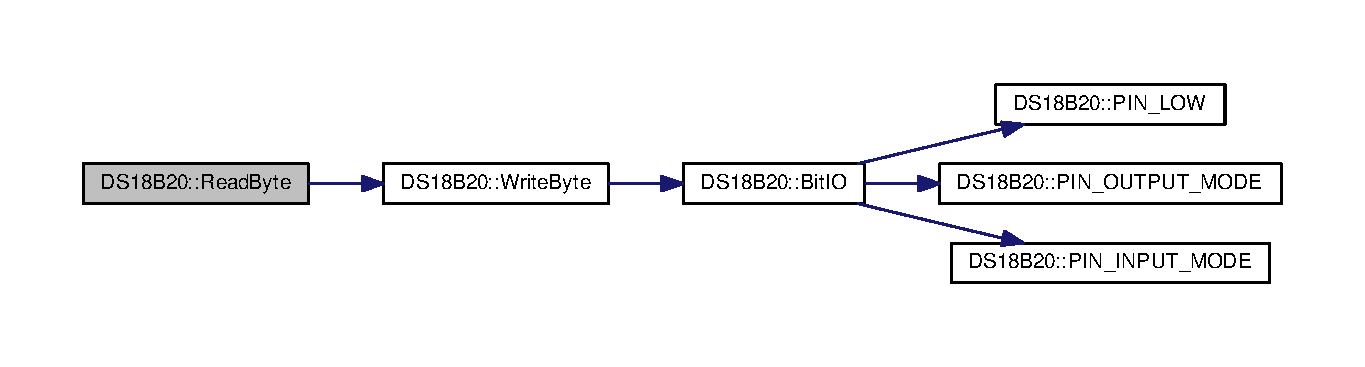
\includegraphics[width=350pt]{classDS18B20_aa43d0c42ebb25bbdc9b7904710652c75_cgraph}
\end{center}
\end{figure}


\index{D\+S18\+B20@{D\+S18\+B20}!Read\+Measurement@{Read\+Measurement}}
\index{Read\+Measurement@{Read\+Measurement}!D\+S18\+B20@{D\+S18\+B20}}
\subsubsection[{\texorpdfstring{Read\+Measurement(char $\ast$string)}{ReadMeasurement(char *string)}}]{\setlength{\rightskip}{0pt plus 5cm}void D\+S18\+B20\+::\+Read\+Measurement (
\begin{DoxyParamCaption}
\item[{char $\ast$}]{string}
\end{DoxyParamCaption}
)}\hypertarget{classDS18B20_a6340d31cea87cf473af13fc7f15f60e4}{}\label{classDS18B20_a6340d31cea87cf473af13fc7f15f60e4}


Takes a Measurement per sensor on the bus. 


\begin{DoxyParams}[1]{Parameters}
\mbox{\tt out}  & {\em string} & String with M\+AC addresses and temperature values \\
\hline
\end{DoxyParams}


Here is the call graph for this function\+:\nopagebreak
\begin{figure}[H]
\begin{center}
\leavevmode
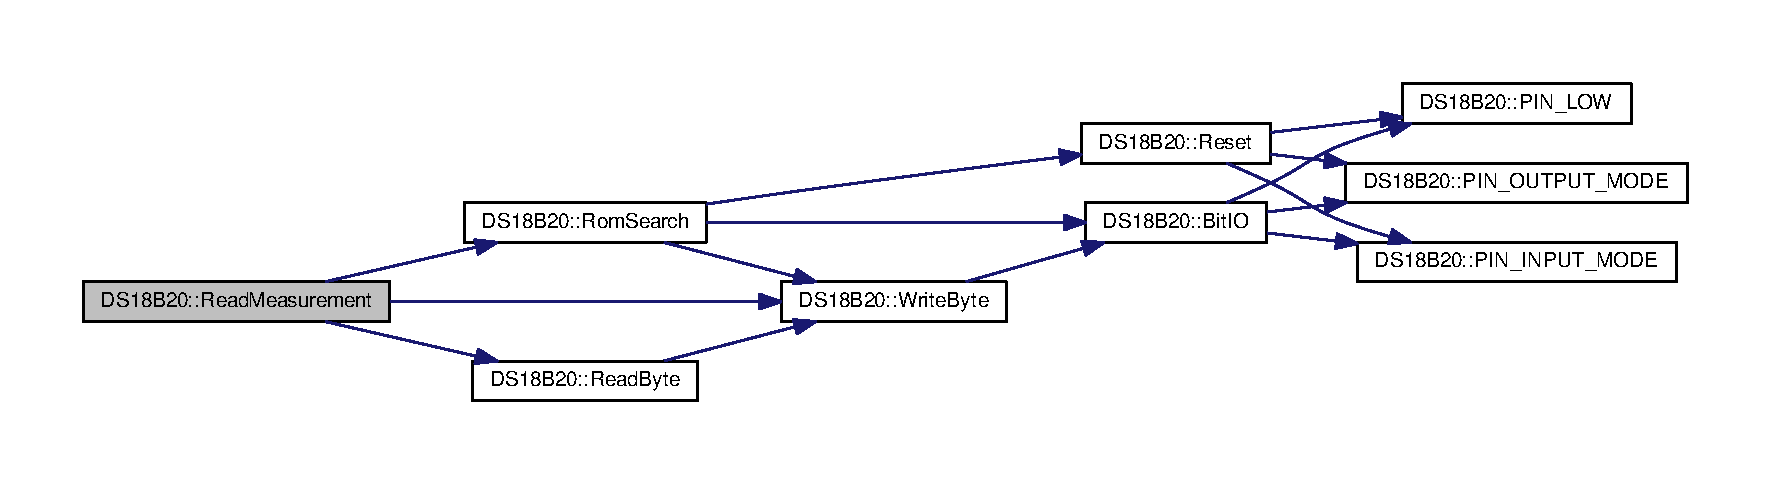
\includegraphics[width=350pt]{classDS18B20_a6340d31cea87cf473af13fc7f15f60e4_cgraph}
\end{center}
\end{figure}


\index{D\+S18\+B20@{D\+S18\+B20}!Read\+Measurement2@{Read\+Measurement2}}
\index{Read\+Measurement2@{Read\+Measurement2}!D\+S18\+B20@{D\+S18\+B20}}
\subsubsection[{\texorpdfstring{Read\+Measurement2(char $\ast$\+Macstring, char $\ast$temp\+Str)}{ReadMeasurement2(char *Macstring, char *tempStr)}}]{\setlength{\rightskip}{0pt plus 5cm}void D\+S18\+B20\+::\+Read\+Measurement2 (
\begin{DoxyParamCaption}
\item[{char $\ast$}]{Macstring, }
\item[{char $\ast$}]{temp\+Str}
\end{DoxyParamCaption}
)}\hypertarget{classDS18B20_a440a17340ac61a693316550422e4ae4e}{}\label{classDS18B20_a440a17340ac61a693316550422e4ae4e}


Takes a Measurement per sensor on the bus. 


\begin{DoxyParams}[1]{Parameters}
\mbox{\tt out}  & {\em Macstring} & M\+AC addresses of each sensor on the bus \\
\hline
\mbox{\tt out}  & {\em temp\+Str} & Temperature values in one string \\
\hline
\end{DoxyParams}


Here is the call graph for this function\+:\nopagebreak
\begin{figure}[H]
\begin{center}
\leavevmode
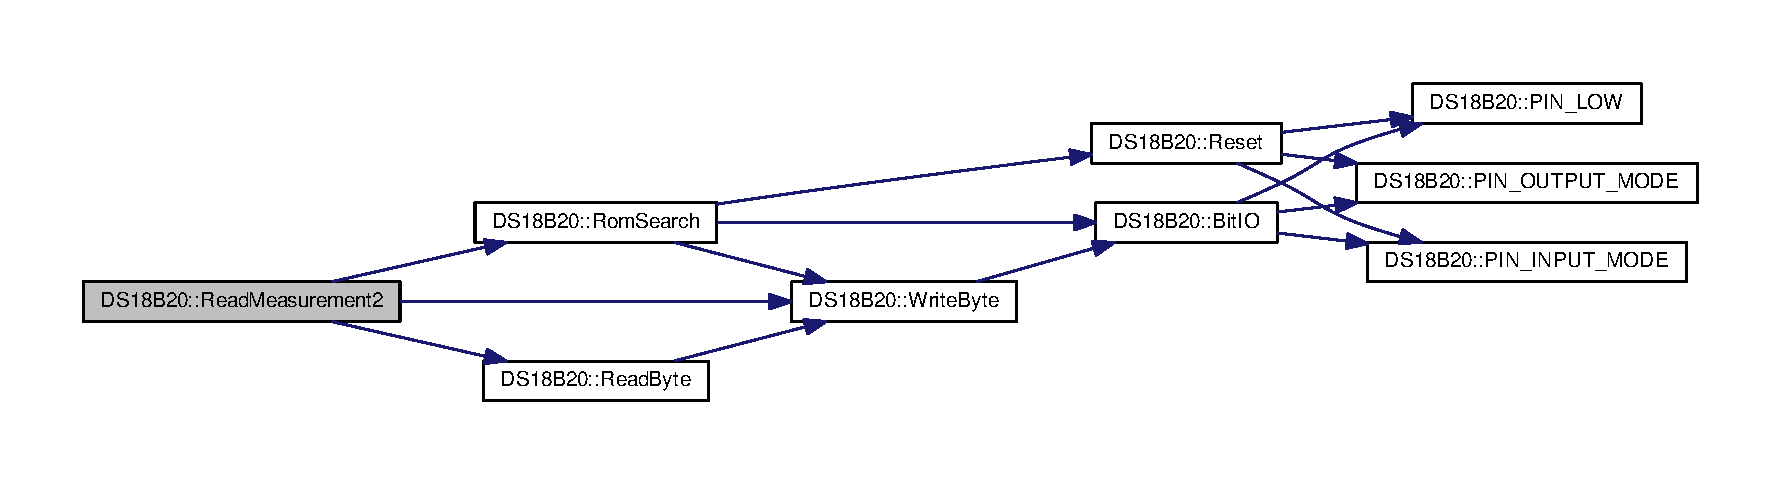
\includegraphics[width=350pt]{classDS18B20_a440a17340ac61a693316550422e4ae4e_cgraph}
\end{center}
\end{figure}


\index{D\+S18\+B20@{D\+S18\+B20}!Reset@{Reset}}
\index{Reset@{Reset}!D\+S18\+B20@{D\+S18\+B20}}
\subsubsection[{\texorpdfstring{Reset()}{Reset()}}]{\setlength{\rightskip}{0pt plus 5cm}uint8\+\_\+t D\+S18\+B20\+::\+Reset (
\begin{DoxyParamCaption}
{}
\end{DoxyParamCaption}
)\hspace{0.3cm}{\ttfamily [private]}}\hypertarget{classDS18B20_a890b94747fbd3ec6e45088735c7bc1fe}{}\label{classDS18B20_a890b94747fbd3ec6e45088735c7bc1fe}


Here is the call graph for this function\+:\nopagebreak
\begin{figure}[H]
\begin{center}
\leavevmode
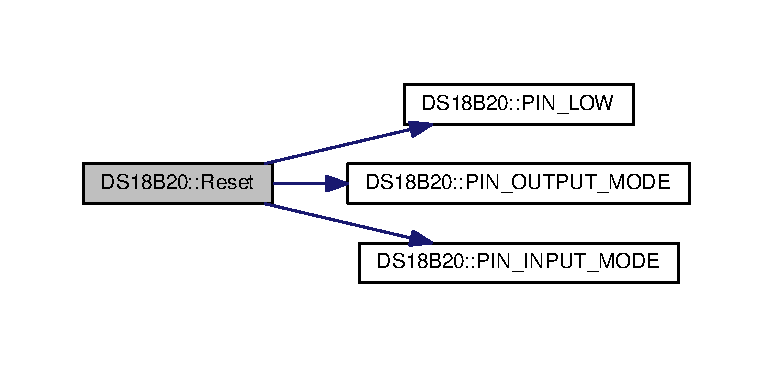
\includegraphics[width=350pt]{classDS18B20_a890b94747fbd3ec6e45088735c7bc1fe_cgraph}
\end{center}
\end{figure}


\index{D\+S18\+B20@{D\+S18\+B20}!Rom\+Search@{Rom\+Search}}
\index{Rom\+Search@{Rom\+Search}!D\+S18\+B20@{D\+S18\+B20}}
\subsubsection[{\texorpdfstring{Rom\+Search(unsigned char diff, unsigned char $\ast$id)}{RomSearch(unsigned char diff, unsigned char *id)}}]{\setlength{\rightskip}{0pt plus 5cm}unsigned char D\+S18\+B20\+::\+Rom\+Search (
\begin{DoxyParamCaption}
\item[{unsigned char}]{diff, }
\item[{unsigned char $\ast$}]{id}
\end{DoxyParamCaption}
)\hspace{0.3cm}{\ttfamily [private]}}\hypertarget{classDS18B20_a356e88e8a6bca4f5ffeb41180c08f91d}{}\label{classDS18B20_a356e88e8a6bca4f5ffeb41180c08f91d}


Here is the call graph for this function\+:\nopagebreak
\begin{figure}[H]
\begin{center}
\leavevmode
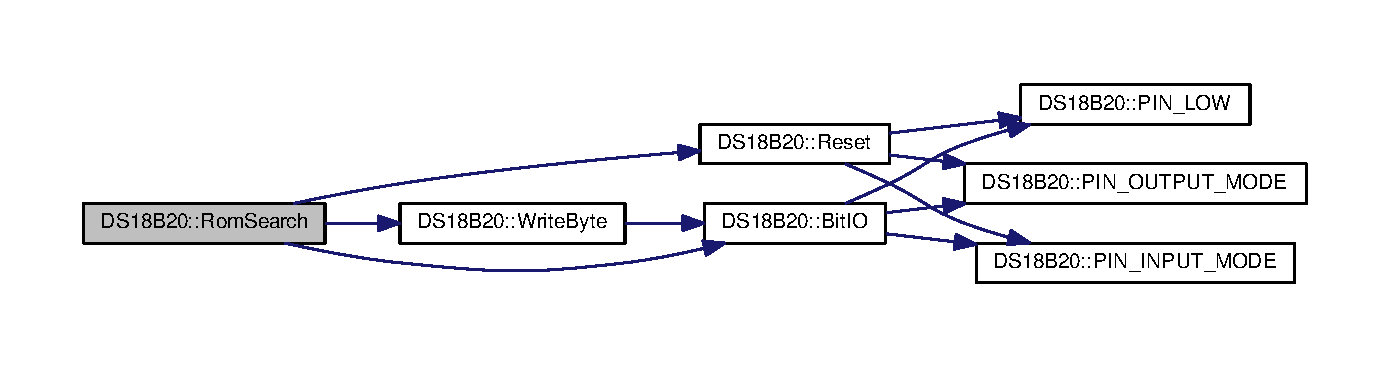
\includegraphics[width=350pt]{classDS18B20_a356e88e8a6bca4f5ffeb41180c08f91d_cgraph}
\end{center}
\end{figure}


\index{D\+S18\+B20@{D\+S18\+B20}!Start\+Measurement@{Start\+Measurement}}
\index{Start\+Measurement@{Start\+Measurement}!D\+S18\+B20@{D\+S18\+B20}}
\subsubsection[{\texorpdfstring{Start\+Measurement(void)}{StartMeasurement(void)}}]{\setlength{\rightskip}{0pt plus 5cm}void D\+S18\+B20\+::\+Start\+Measurement (
\begin{DoxyParamCaption}
\item[{void}]{}
\end{DoxyParamCaption}
)\hspace{0.3cm}{\ttfamily [private]}}\hypertarget{classDS18B20_a817183f6ef9552d6559d58d714e5c804}{}\label{classDS18B20_a817183f6ef9552d6559d58d714e5c804}


Here is the call graph for this function\+:\nopagebreak
\begin{figure}[H]
\begin{center}
\leavevmode
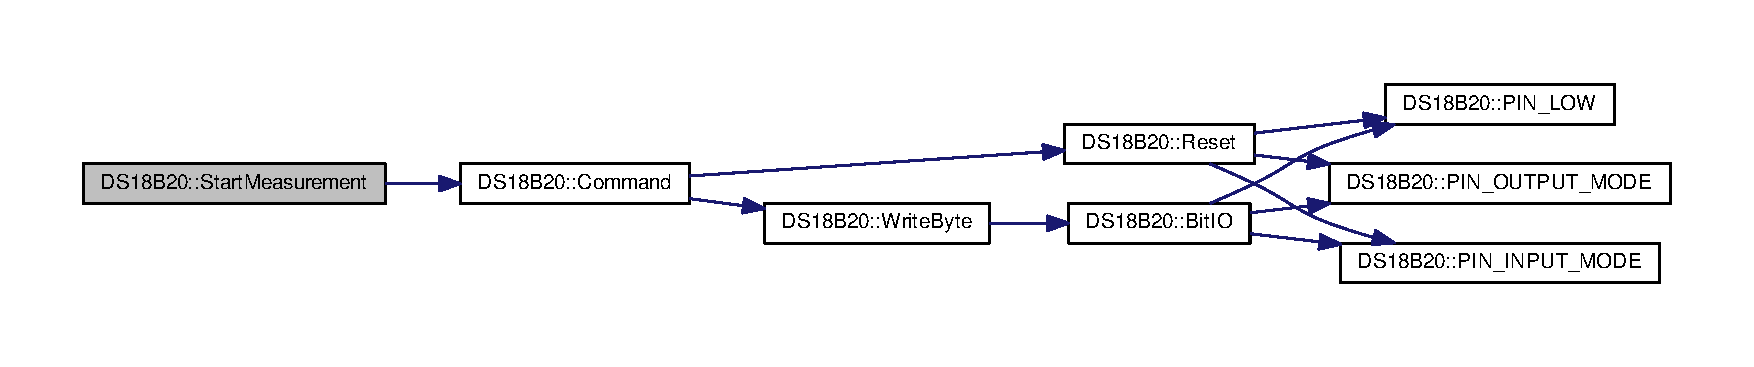
\includegraphics[width=350pt]{classDS18B20_a817183f6ef9552d6559d58d714e5c804_cgraph}
\end{center}
\end{figure}


\index{D\+S18\+B20@{D\+S18\+B20}!Write\+Byte@{Write\+Byte}}
\index{Write\+Byte@{Write\+Byte}!D\+S18\+B20@{D\+S18\+B20}}
\subsubsection[{\texorpdfstring{Write\+Byte(uint8\+\_\+t byte)}{WriteByte(uint8_t byte)}}]{\setlength{\rightskip}{0pt plus 5cm}uint8\+\_\+t D\+S18\+B20\+::\+Write\+Byte (
\begin{DoxyParamCaption}
\item[{uint8\+\_\+t}]{byte}
\end{DoxyParamCaption}
)\hspace{0.3cm}{\ttfamily [private]}}\hypertarget{classDS18B20_a7314cb6a438ddd0c214ed409f7dd5d86}{}\label{classDS18B20_a7314cb6a438ddd0c214ed409f7dd5d86}


Here is the call graph for this function\+:\nopagebreak
\begin{figure}[H]
\begin{center}
\leavevmode
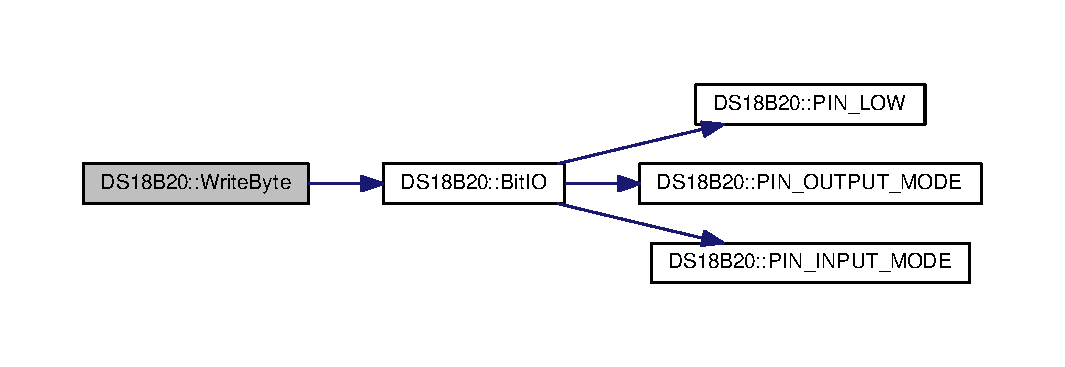
\includegraphics[width=350pt]{classDS18B20_a7314cb6a438ddd0c214ed409f7dd5d86_cgraph}
\end{center}
\end{figure}




\subsection{Member Data Documentation}
\index{D\+S18\+B20@{D\+S18\+B20}!M\+A\+C\+String@{M\+A\+C\+String}}
\index{M\+A\+C\+String@{M\+A\+C\+String}!D\+S18\+B20@{D\+S18\+B20}}
\subsubsection[{\texorpdfstring{M\+A\+C\+String}{MACString}}]{\setlength{\rightskip}{0pt plus 5cm}char D\+S18\+B20\+::\+M\+A\+C\+String\mbox{[}120\mbox{]}\hspace{0.3cm}{\ttfamily [private]}}\hypertarget{classDS18B20_a6884de10b175289718239bdac0b8e52e}{}\label{classDS18B20_a6884de10b175289718239bdac0b8e52e}


M\+AC string of the sensor. 

\index{D\+S18\+B20@{D\+S18\+B20}!W\+I\+R\+E\+\_\+\+D\+DR@{W\+I\+R\+E\+\_\+\+D\+DR}}
\index{W\+I\+R\+E\+\_\+\+D\+DR@{W\+I\+R\+E\+\_\+\+D\+DR}!D\+S18\+B20@{D\+S18\+B20}}
\subsubsection[{\texorpdfstring{W\+I\+R\+E\+\_\+\+D\+DR}{WIRE_DDR}}]{\setlength{\rightskip}{0pt plus 5cm}volatile uint8\+\_\+t$\ast$ D\+S18\+B20\+::\+W\+I\+R\+E\+\_\+\+D\+DR\hspace{0.3cm}{\ttfamily [private]}}\hypertarget{classDS18B20_a06a1f548d087b8d8971dee5e94653f5c}{}\label{classDS18B20_a06a1f548d087b8d8971dee5e94653f5c}


Thermometer data port. 

\index{D\+S18\+B20@{D\+S18\+B20}!W\+I\+R\+E\+\_\+\+DQ@{W\+I\+R\+E\+\_\+\+DQ}}
\index{W\+I\+R\+E\+\_\+\+DQ@{W\+I\+R\+E\+\_\+\+DQ}!D\+S18\+B20@{D\+S18\+B20}}
\subsubsection[{\texorpdfstring{W\+I\+R\+E\+\_\+\+DQ}{WIRE_DQ}}]{\setlength{\rightskip}{0pt plus 5cm}uint8\+\_\+t D\+S18\+B20\+::\+W\+I\+R\+E\+\_\+\+DQ\hspace{0.3cm}{\ttfamily [private]}}\hypertarget{classDS18B20_aebc6a6ab3c604f19dac9a24ef3301938}{}\label{classDS18B20_aebc6a6ab3c604f19dac9a24ef3301938}


Thermometer data line. 

\index{D\+S18\+B20@{D\+S18\+B20}!W\+I\+R\+E\+\_\+\+P\+IN@{W\+I\+R\+E\+\_\+\+P\+IN}}
\index{W\+I\+R\+E\+\_\+\+P\+IN@{W\+I\+R\+E\+\_\+\+P\+IN}!D\+S18\+B20@{D\+S18\+B20}}
\subsubsection[{\texorpdfstring{W\+I\+R\+E\+\_\+\+P\+IN}{WIRE_PIN}}]{\setlength{\rightskip}{0pt plus 5cm}volatile uint8\+\_\+t$\ast$ D\+S18\+B20\+::\+W\+I\+R\+E\+\_\+\+P\+IN\hspace{0.3cm}{\ttfamily [private]}}\hypertarget{classDS18B20_a03a1ad890f9713fc10dc353c9779a7f2}{}\label{classDS18B20_a03a1ad890f9713fc10dc353c9779a7f2}


Thermometer data port. 

\index{D\+S18\+B20@{D\+S18\+B20}!W\+I\+R\+E\+\_\+\+P\+O\+RT@{W\+I\+R\+E\+\_\+\+P\+O\+RT}}
\index{W\+I\+R\+E\+\_\+\+P\+O\+RT@{W\+I\+R\+E\+\_\+\+P\+O\+RT}!D\+S18\+B20@{D\+S18\+B20}}
\subsubsection[{\texorpdfstring{W\+I\+R\+E\+\_\+\+P\+O\+RT}{WIRE_PORT}}]{\setlength{\rightskip}{0pt plus 5cm}volatile uint8\+\_\+t$\ast$ D\+S18\+B20\+::\+W\+I\+R\+E\+\_\+\+P\+O\+RT\hspace{0.3cm}{\ttfamily [private]}}\hypertarget{classDS18B20_a4e8d420cd118999883bde12e766bc1d4}{}\label{classDS18B20_a4e8d420cd118999883bde12e766bc1d4}


Thermometer data port. 



The documentation for this class was generated from the following files\+:\begin{DoxyCompactItemize}
\item 
src/\+Sensors/\hyperlink{DS18B20_8h}{D\+S18\+B20.\+h}\item 
src/\+Sensors/\hyperlink{DS18B20_8cpp}{D\+S18\+B20.\+cpp}\end{DoxyCompactItemize}

\hypertarget{classsensors_1_1LightAnalog}{}\section{sensors.\+Light\+Analog Class Reference}
\label{classsensors_1_1LightAnalog}\index{sensors.\+Light\+Analog@{sensors.\+Light\+Analog}}


Inheritance diagram for sensors.\+Light\+Analog\+:\nopagebreak
\begin{figure}[H]
\begin{center}
\leavevmode
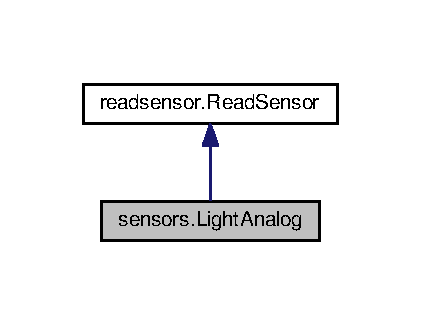
\includegraphics[width=202pt]{classsensors_1_1LightAnalog__inherit__graph}
\end{center}
\end{figure}


Collaboration diagram for sensors.\+Light\+Analog\+:\nopagebreak
\begin{figure}[H]
\begin{center}
\leavevmode
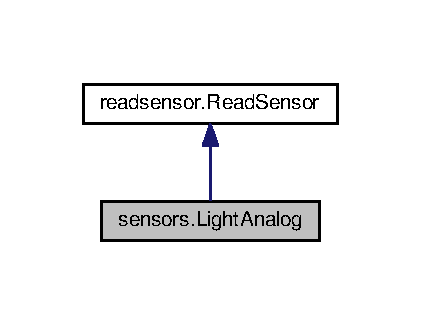
\includegraphics[width=202pt]{classsensors_1_1LightAnalog__coll__graph}
\end{center}
\end{figure}
\subsection*{Public Member Functions}
\begin{DoxyCompactItemize}
\item 
def \hyperlink{classsensors_1_1LightAnalog_a40c88addc7882f729ce0e3564f9096a3}{\+\_\+\+\_\+init\+\_\+\+\_\+} (self, prt, bdrate)
\item 
def \hyperlink{classsensors_1_1LightAnalog_acdc03ffb833d9f66e64261e1c6414e88}{Interpret\+Response} (self)
\item 
def \hyperlink{classsensors_1_1LightAnalog_a9fbb4a2fd317e5229302b5d146204e43}{\+\_\+\+\_\+str\+\_\+\+\_\+} (self)
\end{DoxyCompactItemize}
\subsection*{Public Attributes}
\begin{DoxyCompactItemize}
\item 
\hyperlink{classsensors_1_1LightAnalog_ab1748d35da94bc8da0afead5bded8986}{value}
\item 
\hyperlink{classsensors_1_1LightAnalog_a010099d4873d2f96962dcdf6719364eb}{node\+M\+AC}
\item 
\hyperlink{classsensors_1_1LightAnalog_ac10be263c620f3d2250f6f938d4a8742}{cmd\+ID}
\item 
\hyperlink{classsensors_1_1LightAnalog_ab478dfaacbcb2388fa2ed06394c2cb81}{p\+String}
\item 
\hyperlink{classsensors_1_1LightAnalog_a6c8c998239ae4b79136e58252c631717}{resp\+Mask}
\end{DoxyCompactItemize}


\subsection{Constructor \& Destructor Documentation}
\index{sensors\+::\+Light\+Analog@{sensors\+::\+Light\+Analog}!\+\_\+\+\_\+init\+\_\+\+\_\+@{\+\_\+\+\_\+init\+\_\+\+\_\+}}
\index{\+\_\+\+\_\+init\+\_\+\+\_\+@{\+\_\+\+\_\+init\+\_\+\+\_\+}!sensors\+::\+Light\+Analog@{sensors\+::\+Light\+Analog}}
\subsubsection[{\texorpdfstring{\+\_\+\+\_\+init\+\_\+\+\_\+(self, prt, bdrate)}{__init__(self, prt, bdrate)}}]{\setlength{\rightskip}{0pt plus 5cm}def sensors.\+Light\+Analog.\+\_\+\+\_\+init\+\_\+\+\_\+ (
\begin{DoxyParamCaption}
\item[{}]{self, }
\item[{}]{prt, }
\item[{}]{bdrate}
\end{DoxyParamCaption}
)}\hypertarget{classsensors_1_1LightAnalog_a40c88addc7882f729ce0e3564f9096a3}{}\label{classsensors_1_1LightAnalog_a40c88addc7882f729ce0e3564f9096a3}


Here is the call graph for this function\+:\nopagebreak
\begin{figure}[H]
\begin{center}
\leavevmode
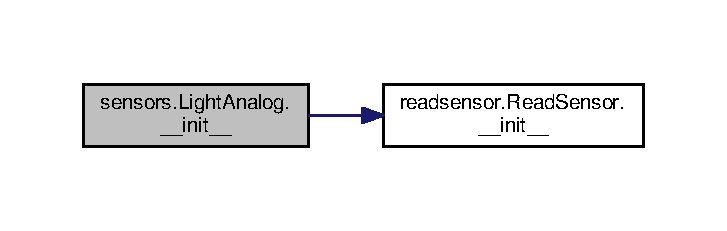
\includegraphics[width=349pt]{classsensors_1_1LightAnalog_a40c88addc7882f729ce0e3564f9096a3_cgraph}
\end{center}
\end{figure}




\subsection{Member Function Documentation}
\index{sensors\+::\+Light\+Analog@{sensors\+::\+Light\+Analog}!\+\_\+\+\_\+str\+\_\+\+\_\+@{\+\_\+\+\_\+str\+\_\+\+\_\+}}
\index{\+\_\+\+\_\+str\+\_\+\+\_\+@{\+\_\+\+\_\+str\+\_\+\+\_\+}!sensors\+::\+Light\+Analog@{sensors\+::\+Light\+Analog}}
\subsubsection[{\texorpdfstring{\+\_\+\+\_\+str\+\_\+\+\_\+(self)}{__str__(self)}}]{\setlength{\rightskip}{0pt plus 5cm}def sensors.\+Light\+Analog.\+\_\+\+\_\+str\+\_\+\+\_\+ (
\begin{DoxyParamCaption}
\item[{}]{self}
\end{DoxyParamCaption}
)}\hypertarget{classsensors_1_1LightAnalog_a9fbb4a2fd317e5229302b5d146204e43}{}\label{classsensors_1_1LightAnalog_a9fbb4a2fd317e5229302b5d146204e43}
\index{sensors\+::\+Light\+Analog@{sensors\+::\+Light\+Analog}!Interpret\+Response@{Interpret\+Response}}
\index{Interpret\+Response@{Interpret\+Response}!sensors\+::\+Light\+Analog@{sensors\+::\+Light\+Analog}}
\subsubsection[{\texorpdfstring{Interpret\+Response(self)}{InterpretResponse(self)}}]{\setlength{\rightskip}{0pt plus 5cm}def sensors.\+Light\+Analog.\+Interpret\+Response (
\begin{DoxyParamCaption}
\item[{}]{self}
\end{DoxyParamCaption}
)}\hypertarget{classsensors_1_1LightAnalog_acdc03ffb833d9f66e64261e1c6414e88}{}\label{classsensors_1_1LightAnalog_acdc03ffb833d9f66e64261e1c6414e88}
\begin{DoxyVerb}Interpret response list \end{DoxyVerb}
 

\subsection{Member Data Documentation}
\index{sensors\+::\+Light\+Analog@{sensors\+::\+Light\+Analog}!cmd\+ID@{cmd\+ID}}
\index{cmd\+ID@{cmd\+ID}!sensors\+::\+Light\+Analog@{sensors\+::\+Light\+Analog}}
\subsubsection[{\texorpdfstring{cmd\+ID}{cmdID}}]{\setlength{\rightskip}{0pt plus 5cm}sensors.\+Light\+Analog.\+cmd\+ID}\hypertarget{classsensors_1_1LightAnalog_ac10be263c620f3d2250f6f938d4a8742}{}\label{classsensors_1_1LightAnalog_ac10be263c620f3d2250f6f938d4a8742}
\index{sensors\+::\+Light\+Analog@{sensors\+::\+Light\+Analog}!node\+M\+AC@{node\+M\+AC}}
\index{node\+M\+AC@{node\+M\+AC}!sensors\+::\+Light\+Analog@{sensors\+::\+Light\+Analog}}
\subsubsection[{\texorpdfstring{node\+M\+AC}{nodeMAC}}]{\setlength{\rightskip}{0pt plus 5cm}sensors.\+Light\+Analog.\+node\+M\+AC}\hypertarget{classsensors_1_1LightAnalog_a010099d4873d2f96962dcdf6719364eb}{}\label{classsensors_1_1LightAnalog_a010099d4873d2f96962dcdf6719364eb}
\index{sensors\+::\+Light\+Analog@{sensors\+::\+Light\+Analog}!p\+String@{p\+String}}
\index{p\+String@{p\+String}!sensors\+::\+Light\+Analog@{sensors\+::\+Light\+Analog}}
\subsubsection[{\texorpdfstring{p\+String}{pString}}]{\setlength{\rightskip}{0pt plus 5cm}sensors.\+Light\+Analog.\+p\+String}\hypertarget{classsensors_1_1LightAnalog_ab478dfaacbcb2388fa2ed06394c2cb81}{}\label{classsensors_1_1LightAnalog_ab478dfaacbcb2388fa2ed06394c2cb81}
\index{sensors\+::\+Light\+Analog@{sensors\+::\+Light\+Analog}!resp\+Mask@{resp\+Mask}}
\index{resp\+Mask@{resp\+Mask}!sensors\+::\+Light\+Analog@{sensors\+::\+Light\+Analog}}
\subsubsection[{\texorpdfstring{resp\+Mask}{respMask}}]{\setlength{\rightskip}{0pt plus 5cm}sensors.\+Light\+Analog.\+resp\+Mask}\hypertarget{classsensors_1_1LightAnalog_a6c8c998239ae4b79136e58252c631717}{}\label{classsensors_1_1LightAnalog_a6c8c998239ae4b79136e58252c631717}
\index{sensors\+::\+Light\+Analog@{sensors\+::\+Light\+Analog}!value@{value}}
\index{value@{value}!sensors\+::\+Light\+Analog@{sensors\+::\+Light\+Analog}}
\subsubsection[{\texorpdfstring{value}{value}}]{\setlength{\rightskip}{0pt plus 5cm}sensors.\+Light\+Analog.\+value}\hypertarget{classsensors_1_1LightAnalog_ab1748d35da94bc8da0afead5bded8986}{}\label{classsensors_1_1LightAnalog_ab1748d35da94bc8da0afead5bded8986}


The documentation for this class was generated from the following file\+:\begin{DoxyCompactItemize}
\item 
Python/\hyperlink{sensors_8py}{sensors.\+py}\end{DoxyCompactItemize}

\hypertarget{classsensors_1_1LightDigital}{}\section{sensors.\+Light\+Digital Class Reference}
\label{classsensors_1_1LightDigital}\index{sensors.\+Light\+Digital@{sensors.\+Light\+Digital}}


Inheritance diagram for sensors.\+Light\+Digital\+:\nopagebreak
\begin{figure}[H]
\begin{center}
\leavevmode
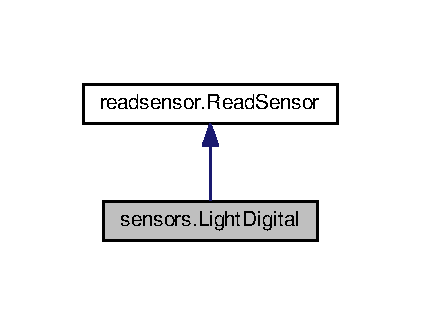
\includegraphics[width=202pt]{classsensors_1_1LightDigital__inherit__graph}
\end{center}
\end{figure}


Collaboration diagram for sensors.\+Light\+Digital\+:\nopagebreak
\begin{figure}[H]
\begin{center}
\leavevmode
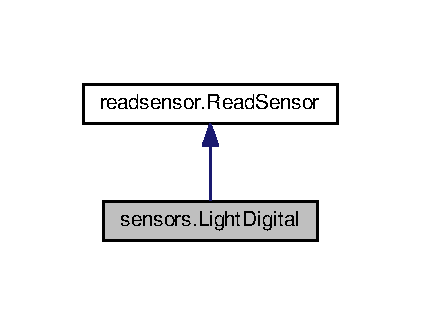
\includegraphics[width=202pt]{classsensors_1_1LightDigital__coll__graph}
\end{center}
\end{figure}
\subsection*{Public Member Functions}
\begin{DoxyCompactItemize}
\item 
def \hyperlink{classsensors_1_1LightDigital_aea795c27407bb29a13affc59590f3d35}{\+\_\+\+\_\+init\+\_\+\+\_\+} (self, prt, bdrate)
\item 
def \hyperlink{classsensors_1_1LightDigital_a9c4ce46c5f389829d0c5e0bfe2a0f2b2}{Interpret\+Response} (self)
\item 
def \hyperlink{classsensors_1_1LightDigital_a41c4038570137761e4f9600e487e3f6b}{\+\_\+\+\_\+str\+\_\+\+\_\+} (self)
\end{DoxyCompactItemize}
\subsection*{Public Attributes}
\begin{DoxyCompactItemize}
\item 
\hyperlink{classsensors_1_1LightDigital_ad801e3eae346e5661ce737ade49e6ac1}{value}
\item 
\hyperlink{classsensors_1_1LightDigital_aff8ca45bed10fa813320e1c9d9c98629}{node\+M\+AC}
\item 
\hyperlink{classsensors_1_1LightDigital_a52e5f8dd9fe1ebde97aa97cbfc36f630}{cmd\+ID}
\item 
\hyperlink{classsensors_1_1LightDigital_a4006bea0c1d6a032afa6285c64ab3eb2}{p\+String}
\item 
\hyperlink{classsensors_1_1LightDigital_a546ea9eee933df95e39666468fb110af}{resp\+Mask}
\end{DoxyCompactItemize}


\subsection{Constructor \& Destructor Documentation}
\index{sensors\+::\+Light\+Digital@{sensors\+::\+Light\+Digital}!\+\_\+\+\_\+init\+\_\+\+\_\+@{\+\_\+\+\_\+init\+\_\+\+\_\+}}
\index{\+\_\+\+\_\+init\+\_\+\+\_\+@{\+\_\+\+\_\+init\+\_\+\+\_\+}!sensors\+::\+Light\+Digital@{sensors\+::\+Light\+Digital}}
\subsubsection[{\texorpdfstring{\+\_\+\+\_\+init\+\_\+\+\_\+(self, prt, bdrate)}{__init__(self, prt, bdrate)}}]{\setlength{\rightskip}{0pt plus 5cm}def sensors.\+Light\+Digital.\+\_\+\+\_\+init\+\_\+\+\_\+ (
\begin{DoxyParamCaption}
\item[{}]{self, }
\item[{}]{prt, }
\item[{}]{bdrate}
\end{DoxyParamCaption}
)}\hypertarget{classsensors_1_1LightDigital_aea795c27407bb29a13affc59590f3d35}{}\label{classsensors_1_1LightDigital_aea795c27407bb29a13affc59590f3d35}


Here is the call graph for this function\+:\nopagebreak
\begin{figure}[H]
\begin{center}
\leavevmode
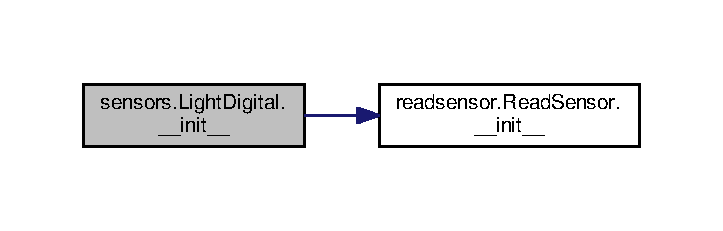
\includegraphics[width=347pt]{classsensors_1_1LightDigital_aea795c27407bb29a13affc59590f3d35_cgraph}
\end{center}
\end{figure}




\subsection{Member Function Documentation}
\index{sensors\+::\+Light\+Digital@{sensors\+::\+Light\+Digital}!\+\_\+\+\_\+str\+\_\+\+\_\+@{\+\_\+\+\_\+str\+\_\+\+\_\+}}
\index{\+\_\+\+\_\+str\+\_\+\+\_\+@{\+\_\+\+\_\+str\+\_\+\+\_\+}!sensors\+::\+Light\+Digital@{sensors\+::\+Light\+Digital}}
\subsubsection[{\texorpdfstring{\+\_\+\+\_\+str\+\_\+\+\_\+(self)}{__str__(self)}}]{\setlength{\rightskip}{0pt plus 5cm}def sensors.\+Light\+Digital.\+\_\+\+\_\+str\+\_\+\+\_\+ (
\begin{DoxyParamCaption}
\item[{}]{self}
\end{DoxyParamCaption}
)}\hypertarget{classsensors_1_1LightDigital_a41c4038570137761e4f9600e487e3f6b}{}\label{classsensors_1_1LightDigital_a41c4038570137761e4f9600e487e3f6b}
\index{sensors\+::\+Light\+Digital@{sensors\+::\+Light\+Digital}!Interpret\+Response@{Interpret\+Response}}
\index{Interpret\+Response@{Interpret\+Response}!sensors\+::\+Light\+Digital@{sensors\+::\+Light\+Digital}}
\subsubsection[{\texorpdfstring{Interpret\+Response(self)}{InterpretResponse(self)}}]{\setlength{\rightskip}{0pt plus 5cm}def sensors.\+Light\+Digital.\+Interpret\+Response (
\begin{DoxyParamCaption}
\item[{}]{self}
\end{DoxyParamCaption}
)}\hypertarget{classsensors_1_1LightDigital_a9c4ce46c5f389829d0c5e0bfe2a0f2b2}{}\label{classsensors_1_1LightDigital_a9c4ce46c5f389829d0c5e0bfe2a0f2b2}
\begin{DoxyVerb}Interpret response list \end{DoxyVerb}
 

\subsection{Member Data Documentation}
\index{sensors\+::\+Light\+Digital@{sensors\+::\+Light\+Digital}!cmd\+ID@{cmd\+ID}}
\index{cmd\+ID@{cmd\+ID}!sensors\+::\+Light\+Digital@{sensors\+::\+Light\+Digital}}
\subsubsection[{\texorpdfstring{cmd\+ID}{cmdID}}]{\setlength{\rightskip}{0pt plus 5cm}sensors.\+Light\+Digital.\+cmd\+ID}\hypertarget{classsensors_1_1LightDigital_a52e5f8dd9fe1ebde97aa97cbfc36f630}{}\label{classsensors_1_1LightDigital_a52e5f8dd9fe1ebde97aa97cbfc36f630}
\index{sensors\+::\+Light\+Digital@{sensors\+::\+Light\+Digital}!node\+M\+AC@{node\+M\+AC}}
\index{node\+M\+AC@{node\+M\+AC}!sensors\+::\+Light\+Digital@{sensors\+::\+Light\+Digital}}
\subsubsection[{\texorpdfstring{node\+M\+AC}{nodeMAC}}]{\setlength{\rightskip}{0pt plus 5cm}sensors.\+Light\+Digital.\+node\+M\+AC}\hypertarget{classsensors_1_1LightDigital_aff8ca45bed10fa813320e1c9d9c98629}{}\label{classsensors_1_1LightDigital_aff8ca45bed10fa813320e1c9d9c98629}
\index{sensors\+::\+Light\+Digital@{sensors\+::\+Light\+Digital}!p\+String@{p\+String}}
\index{p\+String@{p\+String}!sensors\+::\+Light\+Digital@{sensors\+::\+Light\+Digital}}
\subsubsection[{\texorpdfstring{p\+String}{pString}}]{\setlength{\rightskip}{0pt plus 5cm}sensors.\+Light\+Digital.\+p\+String}\hypertarget{classsensors_1_1LightDigital_a4006bea0c1d6a032afa6285c64ab3eb2}{}\label{classsensors_1_1LightDigital_a4006bea0c1d6a032afa6285c64ab3eb2}
\index{sensors\+::\+Light\+Digital@{sensors\+::\+Light\+Digital}!resp\+Mask@{resp\+Mask}}
\index{resp\+Mask@{resp\+Mask}!sensors\+::\+Light\+Digital@{sensors\+::\+Light\+Digital}}
\subsubsection[{\texorpdfstring{resp\+Mask}{respMask}}]{\setlength{\rightskip}{0pt plus 5cm}sensors.\+Light\+Digital.\+resp\+Mask}\hypertarget{classsensors_1_1LightDigital_a546ea9eee933df95e39666468fb110af}{}\label{classsensors_1_1LightDigital_a546ea9eee933df95e39666468fb110af}
\index{sensors\+::\+Light\+Digital@{sensors\+::\+Light\+Digital}!value@{value}}
\index{value@{value}!sensors\+::\+Light\+Digital@{sensors\+::\+Light\+Digital}}
\subsubsection[{\texorpdfstring{value}{value}}]{\setlength{\rightskip}{0pt plus 5cm}sensors.\+Light\+Digital.\+value}\hypertarget{classsensors_1_1LightDigital_ad801e3eae346e5661ce737ade49e6ac1}{}\label{classsensors_1_1LightDigital_ad801e3eae346e5661ce737ade49e6ac1}


The documentation for this class was generated from the following file\+:\begin{DoxyCompactItemize}
\item 
Python/\hyperlink{sensors_8py}{sensors.\+py}\end{DoxyCompactItemize}

\hypertarget{classsensors_1_1Movement}{}\section{sensors.\+Movement Class Reference}
\label{classsensors_1_1Movement}\index{sensors.\+Movement@{sensors.\+Movement}}


Inheritance diagram for sensors.\+Movement\+:\nopagebreak
\begin{figure}[H]
\begin{center}
\leavevmode
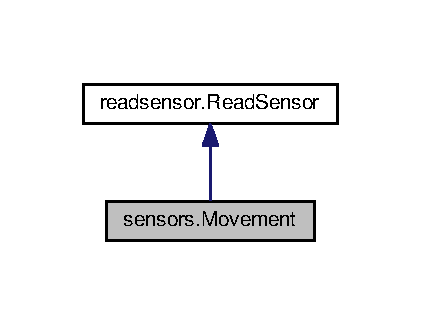
\includegraphics[width=202pt]{classsensors_1_1Movement__inherit__graph}
\end{center}
\end{figure}


Collaboration diagram for sensors.\+Movement\+:\nopagebreak
\begin{figure}[H]
\begin{center}
\leavevmode
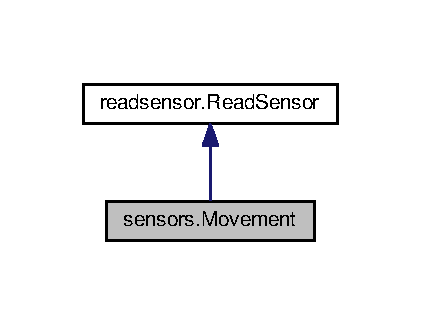
\includegraphics[width=202pt]{classsensors_1_1Movement__coll__graph}
\end{center}
\end{figure}
\subsection*{Public Member Functions}
\begin{DoxyCompactItemize}
\item 
def \hyperlink{classsensors_1_1Movement_a7299348056ba424f565ffe433008411d}{\+\_\+\+\_\+init\+\_\+\+\_\+} (self, prt, bdrate)
\item 
def \hyperlink{classsensors_1_1Movement_a7cffcbdac3bee2a004fcf51366dbd0d1}{Interpret\+Response} (self)
\item 
def \hyperlink{classsensors_1_1Movement_a9f28937de14135f50dd263d05834a535}{\+\_\+\+\_\+str\+\_\+\+\_\+} (self)
\end{DoxyCompactItemize}
\subsection*{Public Attributes}
\begin{DoxyCompactItemize}
\item 
\hyperlink{classsensors_1_1Movement_a11256fb90a76350e4b908a71c72d1e99}{move}
\item 
\hyperlink{classsensors_1_1Movement_abf7c369726a2aacb0e03accdbdcfca14}{node\+M\+AC}
\item 
\hyperlink{classsensors_1_1Movement_abce1eee54738c84ae71c778a4fed1af8}{cmd\+ID}
\item 
\hyperlink{classsensors_1_1Movement_a630da6fa554c8a0d816067d804c02baa}{p\+String}
\item 
\hyperlink{classsensors_1_1Movement_a4f97ac0c0891b427c241df101d7b36ee}{resp\+Mask}
\end{DoxyCompactItemize}


\subsection{Constructor \& Destructor Documentation}
\index{sensors\+::\+Movement@{sensors\+::\+Movement}!\+\_\+\+\_\+init\+\_\+\+\_\+@{\+\_\+\+\_\+init\+\_\+\+\_\+}}
\index{\+\_\+\+\_\+init\+\_\+\+\_\+@{\+\_\+\+\_\+init\+\_\+\+\_\+}!sensors\+::\+Movement@{sensors\+::\+Movement}}
\subsubsection[{\texorpdfstring{\+\_\+\+\_\+init\+\_\+\+\_\+(self, prt, bdrate)}{__init__(self, prt, bdrate)}}]{\setlength{\rightskip}{0pt plus 5cm}def sensors.\+Movement.\+\_\+\+\_\+init\+\_\+\+\_\+ (
\begin{DoxyParamCaption}
\item[{}]{self, }
\item[{}]{prt, }
\item[{}]{bdrate}
\end{DoxyParamCaption}
)}\hypertarget{classsensors_1_1Movement_a7299348056ba424f565ffe433008411d}{}\label{classsensors_1_1Movement_a7299348056ba424f565ffe433008411d}


Here is the call graph for this function\+:\nopagebreak
\begin{figure}[H]
\begin{center}
\leavevmode
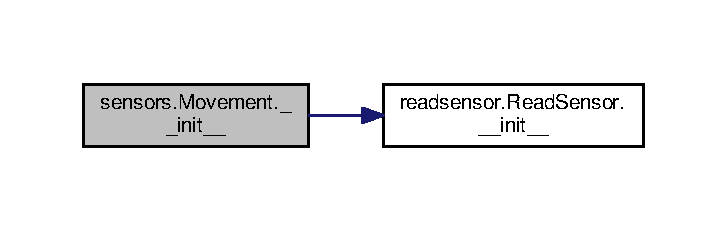
\includegraphics[width=349pt]{classsensors_1_1Movement_a7299348056ba424f565ffe433008411d_cgraph}
\end{center}
\end{figure}




\subsection{Member Function Documentation}
\index{sensors\+::\+Movement@{sensors\+::\+Movement}!\+\_\+\+\_\+str\+\_\+\+\_\+@{\+\_\+\+\_\+str\+\_\+\+\_\+}}
\index{\+\_\+\+\_\+str\+\_\+\+\_\+@{\+\_\+\+\_\+str\+\_\+\+\_\+}!sensors\+::\+Movement@{sensors\+::\+Movement}}
\subsubsection[{\texorpdfstring{\+\_\+\+\_\+str\+\_\+\+\_\+(self)}{__str__(self)}}]{\setlength{\rightskip}{0pt plus 5cm}def sensors.\+Movement.\+\_\+\+\_\+str\+\_\+\+\_\+ (
\begin{DoxyParamCaption}
\item[{}]{self}
\end{DoxyParamCaption}
)}\hypertarget{classsensors_1_1Movement_a9f28937de14135f50dd263d05834a535}{}\label{classsensors_1_1Movement_a9f28937de14135f50dd263d05834a535}
\index{sensors\+::\+Movement@{sensors\+::\+Movement}!Interpret\+Response@{Interpret\+Response}}
\index{Interpret\+Response@{Interpret\+Response}!sensors\+::\+Movement@{sensors\+::\+Movement}}
\subsubsection[{\texorpdfstring{Interpret\+Response(self)}{InterpretResponse(self)}}]{\setlength{\rightskip}{0pt plus 5cm}def sensors.\+Movement.\+Interpret\+Response (
\begin{DoxyParamCaption}
\item[{}]{self}
\end{DoxyParamCaption}
)}\hypertarget{classsensors_1_1Movement_a7cffcbdac3bee2a004fcf51366dbd0d1}{}\label{classsensors_1_1Movement_a7cffcbdac3bee2a004fcf51366dbd0d1}
\begin{DoxyVerb}Interpret response list \end{DoxyVerb}
 

\subsection{Member Data Documentation}
\index{sensors\+::\+Movement@{sensors\+::\+Movement}!cmd\+ID@{cmd\+ID}}
\index{cmd\+ID@{cmd\+ID}!sensors\+::\+Movement@{sensors\+::\+Movement}}
\subsubsection[{\texorpdfstring{cmd\+ID}{cmdID}}]{\setlength{\rightskip}{0pt plus 5cm}sensors.\+Movement.\+cmd\+ID}\hypertarget{classsensors_1_1Movement_abce1eee54738c84ae71c778a4fed1af8}{}\label{classsensors_1_1Movement_abce1eee54738c84ae71c778a4fed1af8}
\index{sensors\+::\+Movement@{sensors\+::\+Movement}!move@{move}}
\index{move@{move}!sensors\+::\+Movement@{sensors\+::\+Movement}}
\subsubsection[{\texorpdfstring{move}{move}}]{\setlength{\rightskip}{0pt plus 5cm}sensors.\+Movement.\+move}\hypertarget{classsensors_1_1Movement_a11256fb90a76350e4b908a71c72d1e99}{}\label{classsensors_1_1Movement_a11256fb90a76350e4b908a71c72d1e99}
\index{sensors\+::\+Movement@{sensors\+::\+Movement}!node\+M\+AC@{node\+M\+AC}}
\index{node\+M\+AC@{node\+M\+AC}!sensors\+::\+Movement@{sensors\+::\+Movement}}
\subsubsection[{\texorpdfstring{node\+M\+AC}{nodeMAC}}]{\setlength{\rightskip}{0pt plus 5cm}sensors.\+Movement.\+node\+M\+AC}\hypertarget{classsensors_1_1Movement_abf7c369726a2aacb0e03accdbdcfca14}{}\label{classsensors_1_1Movement_abf7c369726a2aacb0e03accdbdcfca14}
\index{sensors\+::\+Movement@{sensors\+::\+Movement}!p\+String@{p\+String}}
\index{p\+String@{p\+String}!sensors\+::\+Movement@{sensors\+::\+Movement}}
\subsubsection[{\texorpdfstring{p\+String}{pString}}]{\setlength{\rightskip}{0pt plus 5cm}sensors.\+Movement.\+p\+String}\hypertarget{classsensors_1_1Movement_a630da6fa554c8a0d816067d804c02baa}{}\label{classsensors_1_1Movement_a630da6fa554c8a0d816067d804c02baa}
\index{sensors\+::\+Movement@{sensors\+::\+Movement}!resp\+Mask@{resp\+Mask}}
\index{resp\+Mask@{resp\+Mask}!sensors\+::\+Movement@{sensors\+::\+Movement}}
\subsubsection[{\texorpdfstring{resp\+Mask}{respMask}}]{\setlength{\rightskip}{0pt plus 5cm}sensors.\+Movement.\+resp\+Mask}\hypertarget{classsensors_1_1Movement_a4f97ac0c0891b427c241df101d7b36ee}{}\label{classsensors_1_1Movement_a4f97ac0c0891b427c241df101d7b36ee}


The documentation for this class was generated from the following file\+:\begin{DoxyCompactItemize}
\item 
Python/\hyperlink{sensors_8py}{sensors.\+py}\end{DoxyCompactItemize}

\hypertarget{classNRF24L01}{}\section{N\+R\+F24\+L01 Class Reference}
\label{classNRF24L01}\index{N\+R\+F24\+L01@{N\+R\+F24\+L01}}


{\ttfamily \#include $<$N\+R\+F24\+L01.\+h$>$}



Collaboration diagram for N\+R\+F24\+L01\+:\nopagebreak
\begin{figure}[H]
\begin{center}
\leavevmode
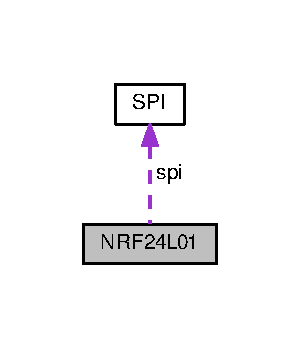
\includegraphics[width=233pt]{classNRF24L01__coll__graph}
\end{center}
\end{figure}
\subsection*{Public Member Functions}
\begin{DoxyCompactItemize}
\item 
\hyperlink{classNRF24L01_ad3e6263e0afaa974637d1450b6c8cb37}{N\+R\+F24\+L01} ()
\item 
\hyperlink{classNRF24L01_a8e8e6754c34cf6e6fed554a6e26c8a4b}{N\+R\+F24\+L01} (\hyperlink{classIO}{IO} $\ast$\hyperlink{classNRF24L01_ae1eea9f32346ecf60ffbf5224d338359}{io\+Interface}, volatile uint8\+\_\+t \&D\+DR, volatile uint8\+\_\+t \&P\+O\+RT, uint8\+\_\+t \hyperlink{main_8cpp_af332f65aca07c44deeda884c8f6c353c}{CE}, uint8\+\_\+t \hyperlink{main_8cpp_a8df4f3a8a2035df063402ae5f0c1d2f8}{C\+SN})
\item 
bool \hyperlink{classNRF24L01_a2973773d1a158e1cfbf52198f248c548}{Init} ()
\item 
void \hyperlink{classNRF24L01_aaabd39829998b609c0dc317af4f141b2}{start\+Listening} ()
\item 
void \hyperlink{classNRF24L01_a6ad13189b732f237ac148c659ddf6b01}{stop\+Listening} ()
\item 
bool \hyperlink{classNRF24L01_ab368039cf5448f0ff5d489563d530c7b}{available} ()
\item 
void \hyperlink{classNRF24L01_a60ed6c6e072a1f41ca560546745ec6da}{read} (void $\ast$buf, uint8\+\_\+t len)
\item 
bool \hyperlink{classNRF24L01_a719390c69a2e45df08379f17e3289f4c}{write} (const void $\ast$buf, uint8\+\_\+t len)
\item 
void \hyperlink{classNRF24L01_ad64a887cae746be5ca43cf08445feed9}{open\+Writing\+Pipe} (const uint8\+\_\+t $\ast$address)
\item 
void \hyperlink{classNRF24L01_a9b458f77f6ae6c42f330710e703dd847}{open\+Reading\+Pipe} (uint8\+\_\+t number, const uint8\+\_\+t $\ast$address)
\end{DoxyCompactItemize}
\subsection*{Private Member Functions}
\begin{Indent}{\bf Low-\/level internal interface.}\par
{\em Protected methods that address the chip directly. Regular users cannot ever call these. They are documented for completeness and for developers who may want to extend this class. }\begin{DoxyCompactItemize}
\item 
uint8\+\_\+t \hyperlink{classNRF24L01_a9766146f8b6bcab59e91e7545484c401}{Read\+Registers} (uint8\+\_\+t reg, uint8\+\_\+t $\ast$buf, uint8\+\_\+t len)
\item 
uint8\+\_\+t \hyperlink{classNRF24L01_a6fc7da02296e9f91908e89438ba67901}{Read\+Register} (uint8\+\_\+t reg)
\item 
uint8\+\_\+t \hyperlink{classNRF24L01_ac7d69c51eca87f16fa3a30b5e8aa85cb}{Write\+Registers} (uint8\+\_\+t reg, const uint8\+\_\+t $\ast$buf, uint8\+\_\+t len)
\item 
uint8\+\_\+t \hyperlink{classNRF24L01_abfaaa54aff7ce60c4c844dd540c47af5}{Write\+Register} (uint8\+\_\+t reg, uint8\+\_\+t value)
\item 
uint8\+\_\+t \hyperlink{classNRF24L01_a9abae657dc54d97b6eb63f33c83e9f59}{Write\+Payload} (const void $\ast$buf, uint8\+\_\+t len, const uint8\+\_\+t write\+Type)
\item 
uint8\+\_\+t \hyperlink{classNRF24L01_ad733911b261f73964817dad526745716}{Read\+Payload} (void $\ast$buf, uint8\+\_\+t len)
\item 
uint8\+\_\+t \hyperlink{classNRF24L01_a83cfc941bafe563f38e183504ee8533c}{Flush\+Rx} (void)
\item 
uint8\+\_\+t \hyperlink{classNRF24L01_a95faa729cb8245516e9eb0248c6d9b0f}{get\+Status} (void)
\item 
void \hyperlink{classNRF24L01_aceeaa16f91d7c5fd6a429a6adf678bd4}{Toggle\+Features} (void)
\item 
uint8\+\_\+t \hyperlink{classNRF24L01_ab604b1e177e4812e33ebc39287503197}{spi\+Trans} (uint8\+\_\+t cmd)
\item 
\hyperlink{classNRF24L01_ad796eb9996a6b528534d1ac2ae2d37cd}{\+\_\+\+\_\+attribute\+\_\+\+\_\+} ((gnu\+\_\+inline)) void delay\+\_\+us(uint16\+\_\+t delay)
\end{DoxyCompactItemize}
\end{Indent}
\subsection*{Private Attributes}
\begin{DoxyCompactItemize}
\item 
\hyperlink{classIO}{IO} $\ast$ \hyperlink{classNRF24L01_ae1eea9f32346ecf60ffbf5224d338359}{io\+Interface}
\item 
volatile uint8\+\_\+t $\ast$ \hyperlink{classNRF24L01_a42ef1a6d858a115327d0a7310aaba57c}{N\+R\+F24\+L01\+\_\+\+D\+DR}
\item 
uint8\+\_\+t \hyperlink{classNRF24L01_a56a20345fcb667fcfc9bc1cb62d5152f}{N\+R\+F24\+L01\+\_\+\+CE}
\item 
uint8\+\_\+t \hyperlink{classNRF24L01_a4d36b61597b9919dd4a0ecdc53526020}{N\+R\+F24\+L01\+\_\+\+C\+SN}
\item 
uint16\+\_\+t \hyperlink{classNRF24L01_a4701641c1e8b3d082deb03f93c84d8c7}{spi\+\_\+speed}
\item 
bool \hyperlink{classNRF24L01_a082a99d802a3f2335da94e67cf8440ea}{p\+\_\+variant}
\item 
uint8\+\_\+t \hyperlink{classNRF24L01_a2f5e84525760899949446db94d225700}{N\+R\+F24\+L01\+\_\+\+CH}
\item 
uint8\+\_\+t \hyperlink{classNRF24L01_a6f035e7c49d8ed5e1ab84242cef0e9be}{N\+R\+F24\+L01\+\_\+\+P\+A\+Y\+L\+O\+AD}
\item 
uint8\+\_\+t \hyperlink{classNRF24L01_af2e0a88f330c86d0cc6c43180f70ecbd}{N\+R\+F24\+L01\+\_\+\+A\+CK}
\item 
uint8\+\_\+t \hyperlink{classNRF24L01_a10c710f3795c47ebde120ca3d975c891}{N\+R\+F24\+L01\+\_\+\+E\+N\+A\+B\+L\+E\+D\+P0}
\item 
uint8\+\_\+t \hyperlink{classNRF24L01_a8ebd82a57efbaa5928a56ba6780740de}{N\+R\+F24\+L01\+\_\+\+E\+N\+A\+B\+L\+E\+D\+P1}
\item 
uint8\+\_\+t \hyperlink{classNRF24L01_aac40f597790cf3a62b382f919f1293ce}{N\+R\+F24\+L01\+\_\+\+E\+N\+A\+B\+L\+E\+D\+P2}
\item 
uint8\+\_\+t \hyperlink{classNRF24L01_aea0d090c7d6da9b137ce4ce3690535e8}{N\+R\+F24\+L01\+\_\+\+E\+N\+A\+B\+L\+E\+D\+P3}
\item 
uint8\+\_\+t \hyperlink{classNRF24L01_a4f19e32ed3324724d3478b9f841a2790}{N\+R\+F24\+L01\+\_\+\+E\+N\+A\+B\+L\+E\+D\+P4}
\item 
uint8\+\_\+t \hyperlink{classNRF24L01_ae77cf1829f80c703e36ef57b6d23e9a9}{N\+R\+F24\+L01\+\_\+\+E\+N\+A\+B\+L\+E\+D\+P5}
\item 
uint8\+\_\+t \hyperlink{classNRF24L01_a0b5c60487c6b715b9f17f968f7958d93}{N\+R\+F24\+L01\+\_\+\+A\+D\+D\+R\+S\+I\+ZE}
\item 
uint8\+\_\+t \hyperlink{classNRF24L01_af836ff0a915587aa40b5eabe4101ea4c}{pipe0\+\_\+reading\+\_\+address} \mbox{[}5\mbox{]}
\item 
uint8\+\_\+t \hyperlink{classNRF24L01_ac798ba6ce52fd4a13eb40ff274818157}{N\+R\+F24\+L01\+\_\+\+R\+F24\+\_\+\+PA}
\item 
uint8\+\_\+t \hyperlink{classNRF24L01_a2dc0073a56f6aca86da205dd720fd132}{N\+R\+F24\+L01\+\_\+\+R\+F24\+\_\+\+S\+P\+E\+ED}
\item 
uint8\+\_\+t \hyperlink{classNRF24L01_af6a260dd55ee5c2f7de7cfac4e91178d}{N\+R\+F24\+L01\+\_\+\+R\+F24\+\_\+\+C\+RC}
\item 
bool \hyperlink{classNRF24L01_ae319d1b6a3d950888d2608cc69efb07c}{dynamic\+\_\+payloads\+\_\+enabled}
\end{DoxyCompactItemize}
\subsection*{Advanced Operation}
\label{_amgrpaf32cf1216e734b82e2b52429dae0bf6}%
 Methods you can use to drive the chip in more advanced ways \begin{DoxyCompactItemize}
\item 
bool \hyperlink{classNRF24L01_a749f38c45c00905b3d8e8c180626bff6}{failure\+Detected}
\item 
void \hyperlink{classNRF24L01_ae5c878a568b54ba045a99b9de377b13b}{print\+Details} (void)
\item 
bool \hyperlink{classNRF24L01_a6bfbb693418e2d60556637b6a3599d05}{available} (uint8\+\_\+t $\ast$pipe\+\_\+num)
\item 
bool \hyperlink{classNRF24L01_aebd4d389685333013b4bd12662c0b411}{rx\+Fifo\+Full} ()
\item 
void \hyperlink{classNRF24L01_abaf0ed9cb5b24890631d7b8bc0e3cd82}{power\+Down} (void)
\item 
void \hyperlink{classNRF24L01_a8e184a0a6ca30fbae69c1331a567deda}{power\+Up} (void)
\item 
bool \hyperlink{classNRF24L01_af59b3fd7aece1ae295a2e634a57d2b02}{write} (const void $\ast$buf, uint8\+\_\+t len, const bool multicast)
\item 
bool \hyperlink{classNRF24L01_a693f48de67c8b11ed5860dc481fcfc99}{write\+Fast} (const void $\ast$buf, uint8\+\_\+t len)
\item 
bool \hyperlink{classNRF24L01_a094a978ed0c7da890c90351bd945fabe}{write\+Fast} (const void $\ast$buf, uint8\+\_\+t len, const bool multicast)
\item 
bool \hyperlink{classNRF24L01_ac2c2500350c3dde0df4f09111f8f1b84}{write\+Blocking} (const void $\ast$buf, uint8\+\_\+t len, uint32\+\_\+t timeout)
\item 
bool \hyperlink{classNRF24L01_a4416a731de8d23cac507e8b69ec2becc}{tx\+Stand\+By} ()
\item 
bool \hyperlink{classNRF24L01_a9351f4bff2196c4f69623f636de7c6a4}{tx\+Stand\+By} (uint32\+\_\+t timeout, bool start\+Tx=0)
\item 
void \hyperlink{classNRF24L01_ae0f4b84a244463e8e594d238a71140c5}{write\+Ack\+Payload} (uint8\+\_\+t pipe, const void $\ast$buf, uint8\+\_\+t len)
\item 
bool \hyperlink{classNRF24L01_a99aae87d62d5097447305d66a0b3281d}{is\+Ack\+Payload\+Available} (void)
\item 
void \hyperlink{classNRF24L01_ad98d10f3759d41e565397aba824d121b}{what\+Happened} (bool \&tx\+\_\+ok, bool \&tx\+\_\+fail, bool \&rx\+\_\+ready)
\item 
void \hyperlink{classNRF24L01_ab1ca9025a8740bc38ad5dd7a427e2d4f}{start\+Fast\+Write} (const void $\ast$buf, uint8\+\_\+t len, const bool multicast, bool start\+Tx=1)
\item 
void \hyperlink{classNRF24L01_a282e44fa8d6ec7542e9d725cf048f6b2}{start\+Write} (const void $\ast$buf, uint8\+\_\+t len, const bool multicast)
\item 
void \hyperlink{classNRF24L01_ad0797d9c6f8ecd9619c9e48168571a01}{re\+Use\+TX} ()
\item 
uint8\+\_\+t \hyperlink{classNRF24L01_ab40eeb5ca2337c5f15992f29ee3b5b18}{Flush\+Tx} (void)
\item 
bool \hyperlink{classNRF24L01_a5e934f8f7d37245264ad16e3c360eca7}{test\+Carrier} (void)
\item 
bool \hyperlink{classNRF24L01_abf1d84ed988aa6c7925ebb712b7c7f60}{test\+R\+PD} (void)
\item 
bool \hyperlink{classNRF24L01_aaddabe35ed60f03a2fb2fb475a3cafb5}{is\+Valid} ()
\item 
void \hyperlink{classNRF24L01_a7214eaa3fcd3b6576d8f290e6ab71955}{close\+Reading\+Pipe} (uint8\+\_\+t pipe)
\end{DoxyCompactItemize}
\subsection*{Optional Configurators}
\label{_amgrpe1a83b99ec8153e5baf680edeeed1586}%
 Methods you can use to get or set the configuration of the chip. None are required. Calling begin() sets up a reasonable set of defaults. \begin{DoxyCompactItemize}
\item 
uint32\+\_\+t \hyperlink{classNRF24L01_a1feaab910ecff17805f8141fe40028e7}{tx\+Delay}
\item 
uint32\+\_\+t \hyperlink{classNRF24L01_abae8b8afbf747344006d6163c607be00}{cs\+Delay}
\item 
void \hyperlink{classNRF24L01_a17752733515f67aa9f6ed3daa1ed3d1d}{set\+Address\+Width} (uint8\+\_\+t a\+\_\+width)
\item 
void \hyperlink{classNRF24L01_a0bb209d94b62e2a28af53179af713f3c}{set\+Retries} (uint8\+\_\+t delay, uint8\+\_\+t count)
\item 
void \hyperlink{classNRF24L01_aa8eaf9d5ed604f60a00cd79fed9edad7}{set\+Channel} (uint8\+\_\+t channel)
\item 
uint8\+\_\+t \hyperlink{classNRF24L01_a6b269b519d57d54d0682a29ce9036b12}{get\+Channel} (void)
\item 
void \hyperlink{classNRF24L01_abe5983a57d0d3bd77508e5345774c890}{set\+Payload\+Size} (uint8\+\_\+t size)
\item 
uint8\+\_\+t \hyperlink{classNRF24L01_a4a7f48ca92e14baabd8be1c0831e8c2f}{get\+Payload\+Size} (void)
\item 
uint8\+\_\+t \hyperlink{classNRF24L01_a0d0cd5dd09d60e06280f378166725d64}{get\+Dynamic\+Payload\+Size} (void)
\item 
void \hyperlink{classNRF24L01_ae4067455572c6731211315b3900f5cbd}{enable\+Ack\+Payload} (void)
\item 
void \hyperlink{classNRF24L01_abd060c4df7efac781ed5812a0ee19d08}{enable\+Dynamic\+Payloads} (void)
\item 
void \hyperlink{classNRF24L01_abf6bf0c18b2b12674cfbc150a2bdb778}{disable\+Dynamic\+Payloads} (void)
\item 
void \hyperlink{classNRF24L01_aeaa968ea74bfd2690fff331e9f115344}{enable\+Dynamic\+Ack} ()
\item 
bool \hyperlink{classNRF24L01_ad05024c9586c1dc76c2fd95d54ce6b4c}{is\+P\+Variant} (void)
\item 
void \hyperlink{classNRF24L01_a33b1c7dd1cad95dae57ef87bf3dce5c8}{set\+Auto\+Ack} (bool enable)
\item 
void \hyperlink{classNRF24L01_a79cab6f958c8d9e18273d7c4750480fd}{set\+Auto\+Ack} (uint8\+\_\+t pipe, bool enable)
\item 
void \hyperlink{classNRF24L01_a7319961d6048e32546ad5df934bd42d8}{set\+P\+A\+Level} (uint8\+\_\+t level)
\item 
uint8\+\_\+t \hyperlink{classNRF24L01_a8fdb80b79100186afad90d9a2a5c79fb}{get\+P\+A\+Level} (void)
\item 
bool \hyperlink{classNRF24L01_a9db0803c6d87e6ada7febea2240a7b1c}{set\+Data\+Rate} (uint8\+\_\+t speed)
\item 
\hyperlink{NRF24L01_8h_a82745de4aa1251b7561564b3ed1d6522}{rf24\+\_\+datarate\+\_\+e} \hyperlink{classNRF24L01_a6184de85c94400cde96b7f83b316efa8}{get\+Data\+Rate} (void)
\item 
void \hyperlink{classNRF24L01_a6081dd6dd9cdffbc1c7534ee1824201d}{set\+C\+R\+C\+Length} (uint8\+\_\+t length)
\item 
\hyperlink{NRF24L01_8h_adbe00719f3f835c82bd007081d040a7e}{rf24\+\_\+crclength\+\_\+e} \hyperlink{classNRF24L01_ac83fb86df156475aeda2ef637078fcd3}{get\+C\+R\+C\+Length} (void)
\item 
void \hyperlink{classNRF24L01_a1e997f3c946acdbe8bd622e431f80034}{disable\+C\+RC} (void)
\item 
void \hyperlink{classNRF24L01_ad23d4111c3a26d18db51eb72a5491dbb}{mask\+I\+RQ} (bool tx\+\_\+ok, bool tx\+\_\+fail, bool rx\+\_\+ready)
\item 
void \hyperlink{classNRF24L01_a02c91592a6c762c1a4e86252f8958bd6}{open\+Reading\+Pipe} (uint8\+\_\+t number, uint64\+\_\+t address)
\item 
void \hyperlink{classNRF24L01_a0fe37f8ff95b7c562ad1fc277890e29a}{open\+Writing\+Pipe} (uint64\+\_\+t address)
\item 
void \hyperlink{classNRF24L01_ad311ef5130c99ab8ddca292adfe76603}{delay\+\_\+ms} (uint16\+\_\+t ms)
\item 
void \hyperlink{classNRF24L01_a958fa3e8a0457c0c655b9652ee9dbad4}{C\+S\+N\+\_\+\+H\+I\+GH} ()
\item 
void \hyperlink{classNRF24L01_acffaad2c6b5e3713f7fe6af22d4553ef}{C\+S\+N\+\_\+\+L\+OW} ()
\item 
void \hyperlink{classNRF24L01_a85274c10cbe6317796a209913bfb0253}{C\+E\+\_\+\+H\+I\+GH} ()
\item 
void \hyperlink{classNRF24L01_aa5e261363986c590c90e7cb2adc2d75d}{C\+E\+\_\+\+L\+OW} ()
\end{DoxyCompactItemize}


\subsection{Detailed Description}
Driver for n\+R\+F24\+L01(+) 2.\+4\+G\+Hz Wireless Transceiver 

\subsection{Constructor \& Destructor Documentation}
\index{N\+R\+F24\+L01@{N\+R\+F24\+L01}!N\+R\+F24\+L01@{N\+R\+F24\+L01}}
\index{N\+R\+F24\+L01@{N\+R\+F24\+L01}!N\+R\+F24\+L01@{N\+R\+F24\+L01}}
\subsubsection[{\texorpdfstring{N\+R\+F24\+L01()}{NRF24L01()}}]{\setlength{\rightskip}{0pt plus 5cm}N\+R\+F24\+L01\+::\+N\+R\+F24\+L01 (
\begin{DoxyParamCaption}
{}
\end{DoxyParamCaption}
)}\hypertarget{classNRF24L01_ad3e6263e0afaa974637d1450b6c8cb37}{}\label{classNRF24L01_ad3e6263e0afaa974637d1450b6c8cb37}


Here is the call graph for this function\+:\nopagebreak
\begin{figure}[H]
\begin{center}
\leavevmode
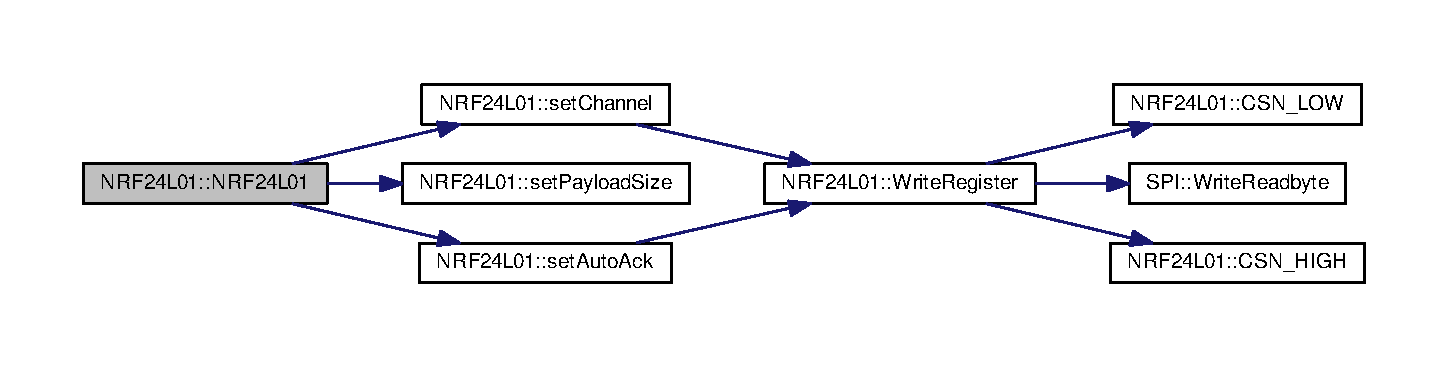
\includegraphics[width=350pt]{classNRF24L01_ad3e6263e0afaa974637d1450b6c8cb37_cgraph}
\end{center}
\end{figure}


\index{N\+R\+F24\+L01@{N\+R\+F24\+L01}!N\+R\+F24\+L01@{N\+R\+F24\+L01}}
\index{N\+R\+F24\+L01@{N\+R\+F24\+L01}!N\+R\+F24\+L01@{N\+R\+F24\+L01}}
\subsubsection[{\texorpdfstring{N\+R\+F24\+L01(\+I\+O $\ast$io\+Interface, volatile uint8\+\_\+t \&\+D\+D\+R, volatile uint8\+\_\+t \&\+P\+O\+R\+T, uint8\+\_\+t C\+E, uint8\+\_\+t C\+S\+N)}{NRF24L01(IO *ioInterface, volatile uint8_t &DDR, volatile uint8_t &PORT, uint8_t CE, uint8_t CSN)}}]{\setlength{\rightskip}{0pt plus 5cm}N\+R\+F24\+L01\+::\+N\+R\+F24\+L01 (
\begin{DoxyParamCaption}
\item[{{\bf IO} $\ast$}]{io\+Interface, }
\item[{volatile uint8\+\_\+t \&}]{D\+DR, }
\item[{volatile uint8\+\_\+t \&}]{P\+O\+RT, }
\item[{uint8\+\_\+t}]{CE, }
\item[{uint8\+\_\+t}]{C\+SN}
\end{DoxyParamCaption}
)}\hypertarget{classNRF24L01_a8e8e6754c34cf6e6fed554a6e26c8a4b}{}\label{classNRF24L01_a8e8e6754c34cf6e6fed554a6e26c8a4b}


\subsection{Member Function Documentation}
\index{N\+R\+F24\+L01@{N\+R\+F24\+L01}!\+\_\+\+\_\+attribute\+\_\+\+\_\+@{\+\_\+\+\_\+attribute\+\_\+\+\_\+}}
\index{\+\_\+\+\_\+attribute\+\_\+\+\_\+@{\+\_\+\+\_\+attribute\+\_\+\+\_\+}!N\+R\+F24\+L01@{N\+R\+F24\+L01}}
\subsubsection[{\texorpdfstring{\+\_\+\+\_\+attribute\+\_\+\+\_\+((gnu\+\_\+inline)) void delay\+\_\+us(uint16\+\_\+t delay)}{__attribute__((gnu_inline)) void delay_us(uint16_t delay)}}]{\setlength{\rightskip}{0pt plus 5cm}N\+R\+F24\+L01\+::\+\_\+\+\_\+attribute\+\_\+\+\_\+ (
\begin{DoxyParamCaption}
\item[{(gnu\+\_\+inline)}]{}
\end{DoxyParamCaption}
)\hspace{0.3cm}{\ttfamily [inline]}, {\ttfamily [private]}}\hypertarget{classNRF24L01_ad796eb9996a6b528534d1ac2ae2d37cd}{}\label{classNRF24L01_ad796eb9996a6b528534d1ac2ae2d37cd}
\index{N\+R\+F24\+L01@{N\+R\+F24\+L01}!available@{available}}
\index{available@{available}!N\+R\+F24\+L01@{N\+R\+F24\+L01}}
\subsubsection[{\texorpdfstring{available()}{available()}}]{\setlength{\rightskip}{0pt plus 5cm}bool N\+R\+F24\+L01\+::available (
\begin{DoxyParamCaption}
\item[{void}]{}
\end{DoxyParamCaption}
)}\hypertarget{classNRF24L01_ab368039cf5448f0ff5d489563d530c7b}{}\label{classNRF24L01_ab368039cf5448f0ff5d489563d530c7b}
Check whether there are bytes available to be read 
\begin{DoxyCode}
\textcolor{keywordflow}{if}(radio.available())\{
  radio.read(&data,\textcolor{keyword}{sizeof}(data));
\}
\end{DoxyCode}
 \begin{DoxyReturn}{Returns}
True if there is a payload available, false if none is 
\end{DoxyReturn}
\index{N\+R\+F24\+L01@{N\+R\+F24\+L01}!available@{available}}
\index{available@{available}!N\+R\+F24\+L01@{N\+R\+F24\+L01}}
\subsubsection[{\texorpdfstring{available(uint8\+\_\+t $\ast$pipe\+\_\+num)}{available(uint8_t *pipe_num)}}]{\setlength{\rightskip}{0pt plus 5cm}bool N\+R\+F24\+L01\+::available (
\begin{DoxyParamCaption}
\item[{uint8\+\_\+t $\ast$}]{pipe\+\_\+num}
\end{DoxyParamCaption}
)}\hypertarget{classNRF24L01_a6bfbb693418e2d60556637b6a3599d05}{}\label{classNRF24L01_a6bfbb693418e2d60556637b6a3599d05}
Test whether there are bytes available to be read in the F\+I\+FO buffers.


\begin{DoxyParams}[1]{Parameters}
\mbox{\tt out}  & {\em pipe\+\_\+num} & Which pipe has the payload available\\
\hline
\end{DoxyParams}

\begin{DoxyCode}
uint8\_t pipeNum;
\textcolor{keywordflow}{if}(radio.available(&pipeNum))\{
  radio.read(&data,\textcolor{keyword}{sizeof}(data));
  Serial.print(\textcolor{stringliteral}{"Got data on pipe"});
  Serial.println(pipeNum);
\}
\end{DoxyCode}
 \begin{DoxyReturn}{Returns}
True if there is a payload available, false if none is 
\end{DoxyReturn}


Here is the call graph for this function\+:\nopagebreak
\begin{figure}[H]
\begin{center}
\leavevmode
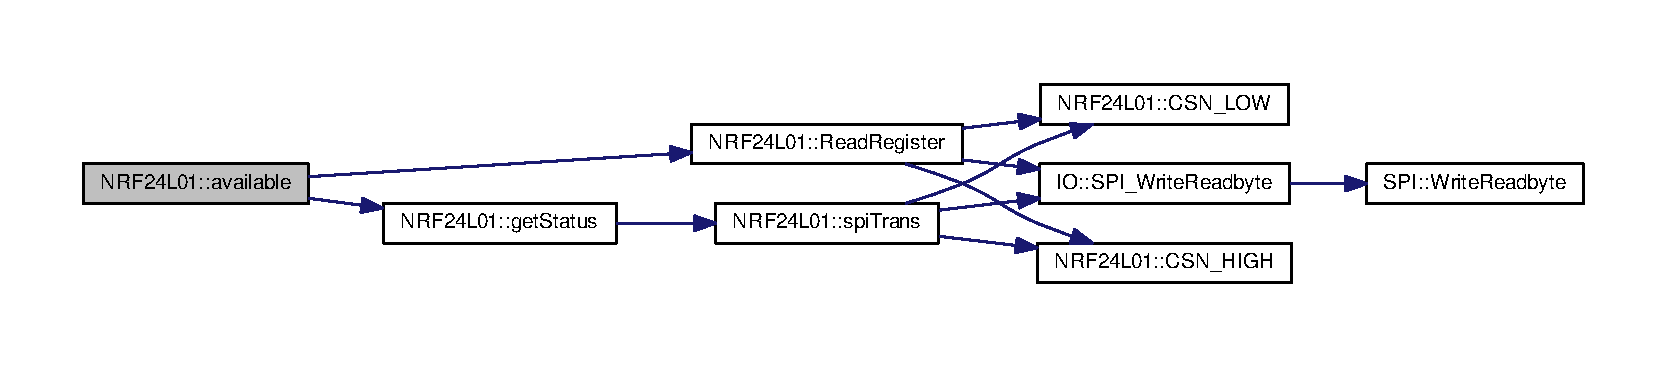
\includegraphics[width=350pt]{classNRF24L01_a6bfbb693418e2d60556637b6a3599d05_cgraph}
\end{center}
\end{figure}


\index{N\+R\+F24\+L01@{N\+R\+F24\+L01}!C\+E\+\_\+\+H\+I\+GH@{C\+E\+\_\+\+H\+I\+GH}}
\index{C\+E\+\_\+\+H\+I\+GH@{C\+E\+\_\+\+H\+I\+GH}!N\+R\+F24\+L01@{N\+R\+F24\+L01}}
\subsubsection[{\texorpdfstring{C\+E\+\_\+\+H\+I\+G\+H()}{CE_HIGH()}}]{\setlength{\rightskip}{0pt plus 5cm}void N\+R\+F24\+L01\+::\+C\+E\+\_\+\+H\+I\+GH (
\begin{DoxyParamCaption}
{}
\end{DoxyParamCaption}
)\hspace{0.3cm}{\ttfamily [inline]}, {\ttfamily [private]}}\hypertarget{classNRF24L01_a85274c10cbe6317796a209913bfb0253}{}\label{classNRF24L01_a85274c10cbe6317796a209913bfb0253}
\index{N\+R\+F24\+L01@{N\+R\+F24\+L01}!C\+E\+\_\+\+L\+OW@{C\+E\+\_\+\+L\+OW}}
\index{C\+E\+\_\+\+L\+OW@{C\+E\+\_\+\+L\+OW}!N\+R\+F24\+L01@{N\+R\+F24\+L01}}
\subsubsection[{\texorpdfstring{C\+E\+\_\+\+L\+O\+W()}{CE_LOW()}}]{\setlength{\rightskip}{0pt plus 5cm}void N\+R\+F24\+L01\+::\+C\+E\+\_\+\+L\+OW (
\begin{DoxyParamCaption}
{}
\end{DoxyParamCaption}
)\hspace{0.3cm}{\ttfamily [inline]}, {\ttfamily [private]}}\hypertarget{classNRF24L01_aa5e261363986c590c90e7cb2adc2d75d}{}\label{classNRF24L01_aa5e261363986c590c90e7cb2adc2d75d}


Here is the call graph for this function\+:\nopagebreak
\begin{figure}[H]
\begin{center}
\leavevmode
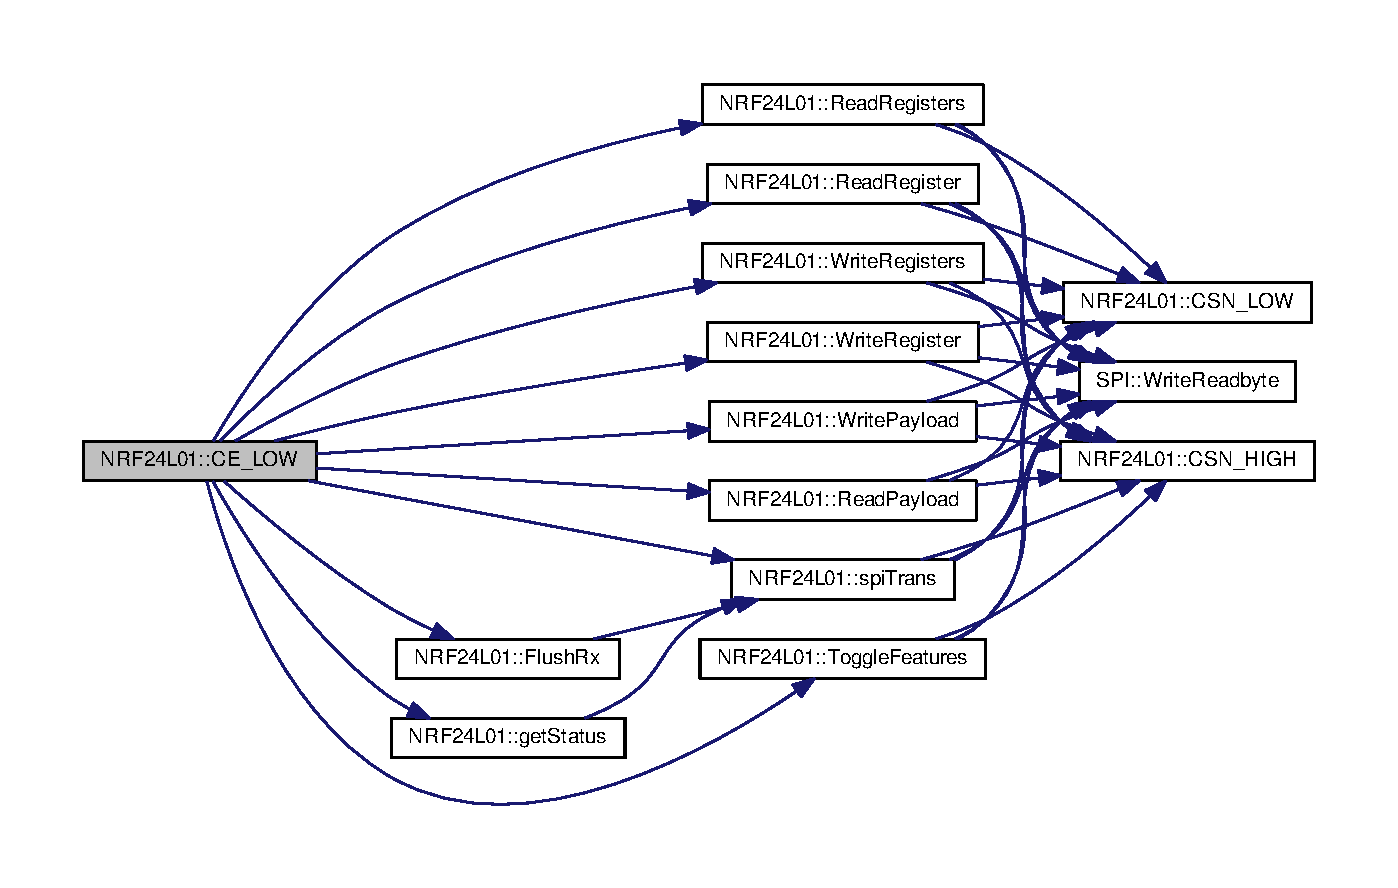
\includegraphics[width=350pt]{classNRF24L01_aa5e261363986c590c90e7cb2adc2d75d_cgraph}
\end{center}
\end{figure}


\index{N\+R\+F24\+L01@{N\+R\+F24\+L01}!close\+Reading\+Pipe@{close\+Reading\+Pipe}}
\index{close\+Reading\+Pipe@{close\+Reading\+Pipe}!N\+R\+F24\+L01@{N\+R\+F24\+L01}}
\subsubsection[{\texorpdfstring{close\+Reading\+Pipe(uint8\+\_\+t pipe)}{closeReadingPipe(uint8_t pipe)}}]{\setlength{\rightskip}{0pt plus 5cm}void N\+R\+F24\+L01\+::close\+Reading\+Pipe (
\begin{DoxyParamCaption}
\item[{uint8\+\_\+t}]{pipe}
\end{DoxyParamCaption}
)}\hypertarget{classNRF24L01_a7214eaa3fcd3b6576d8f290e6ab71955}{}\label{classNRF24L01_a7214eaa3fcd3b6576d8f290e6ab71955}
Close a pipe after it has been previously opened. Can be safely called without having previously opened a pipe. 
\begin{DoxyParams}{Parameters}
{\em pipe} & Which pipe \# to close, 0-\/5. \\
\hline
\end{DoxyParams}


Here is the call graph for this function\+:\nopagebreak
\begin{figure}[H]
\begin{center}
\leavevmode
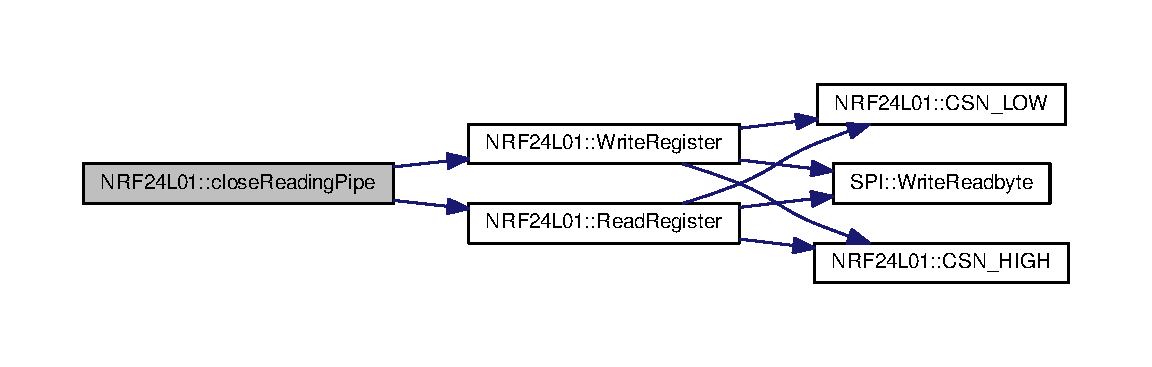
\includegraphics[width=350pt]{classNRF24L01_a7214eaa3fcd3b6576d8f290e6ab71955_cgraph}
\end{center}
\end{figure}


\index{N\+R\+F24\+L01@{N\+R\+F24\+L01}!C\+S\+N\+\_\+\+H\+I\+GH@{C\+S\+N\+\_\+\+H\+I\+GH}}
\index{C\+S\+N\+\_\+\+H\+I\+GH@{C\+S\+N\+\_\+\+H\+I\+GH}!N\+R\+F24\+L01@{N\+R\+F24\+L01}}
\subsubsection[{\texorpdfstring{C\+S\+N\+\_\+\+H\+I\+G\+H()}{CSN_HIGH()}}]{\setlength{\rightskip}{0pt plus 5cm}void N\+R\+F24\+L01\+::\+C\+S\+N\+\_\+\+H\+I\+GH (
\begin{DoxyParamCaption}
{}
\end{DoxyParamCaption}
)\hspace{0.3cm}{\ttfamily [inline]}, {\ttfamily [private]}}\hypertarget{classNRF24L01_a958fa3e8a0457c0c655b9652ee9dbad4}{}\label{classNRF24L01_a958fa3e8a0457c0c655b9652ee9dbad4}
\index{N\+R\+F24\+L01@{N\+R\+F24\+L01}!C\+S\+N\+\_\+\+L\+OW@{C\+S\+N\+\_\+\+L\+OW}}
\index{C\+S\+N\+\_\+\+L\+OW@{C\+S\+N\+\_\+\+L\+OW}!N\+R\+F24\+L01@{N\+R\+F24\+L01}}
\subsubsection[{\texorpdfstring{C\+S\+N\+\_\+\+L\+O\+W()}{CSN_LOW()}}]{\setlength{\rightskip}{0pt plus 5cm}void N\+R\+F24\+L01\+::\+C\+S\+N\+\_\+\+L\+OW (
\begin{DoxyParamCaption}
{}
\end{DoxyParamCaption}
)\hspace{0.3cm}{\ttfamily [inline]}, {\ttfamily [private]}}\hypertarget{classNRF24L01_acffaad2c6b5e3713f7fe6af22d4553ef}{}\label{classNRF24L01_acffaad2c6b5e3713f7fe6af22d4553ef}
\index{N\+R\+F24\+L01@{N\+R\+F24\+L01}!delay\+\_\+ms@{delay\+\_\+ms}}
\index{delay\+\_\+ms@{delay\+\_\+ms}!N\+R\+F24\+L01@{N\+R\+F24\+L01}}
\subsubsection[{\texorpdfstring{delay\+\_\+ms(uint16\+\_\+t ms)}{delay_ms(uint16_t ms)}}]{\setlength{\rightskip}{0pt plus 5cm}void N\+R\+F24\+L01\+::delay\+\_\+ms (
\begin{DoxyParamCaption}
\item[{uint16\+\_\+t}]{ms}
\end{DoxyParamCaption}
)\hspace{0.3cm}{\ttfamily [inline]}, {\ttfamily [private]}}\hypertarget{classNRF24L01_ad311ef5130c99ab8ddca292adfe76603}{}\label{classNRF24L01_ad311ef5130c99ab8ddca292adfe76603}
\index{N\+R\+F24\+L01@{N\+R\+F24\+L01}!disable\+C\+RC@{disable\+C\+RC}}
\index{disable\+C\+RC@{disable\+C\+RC}!N\+R\+F24\+L01@{N\+R\+F24\+L01}}
\subsubsection[{\texorpdfstring{disable\+C\+R\+C(void)}{disableCRC(void)}}]{\setlength{\rightskip}{0pt plus 5cm}void N\+R\+F24\+L01\+::disable\+C\+RC (
\begin{DoxyParamCaption}
\item[{void}]{}
\end{DoxyParamCaption}
)}\hypertarget{classNRF24L01_a1e997f3c946acdbe8bd622e431f80034}{}\label{classNRF24L01_a1e997f3c946acdbe8bd622e431f80034}
Disable C\+RC validation

\begin{DoxyWarning}{Warning}
C\+RC cannot be disabled if auto-\/ack/\+E\+SB is enabled. 
\end{DoxyWarning}


Here is the call graph for this function\+:\nopagebreak
\begin{figure}[H]
\begin{center}
\leavevmode
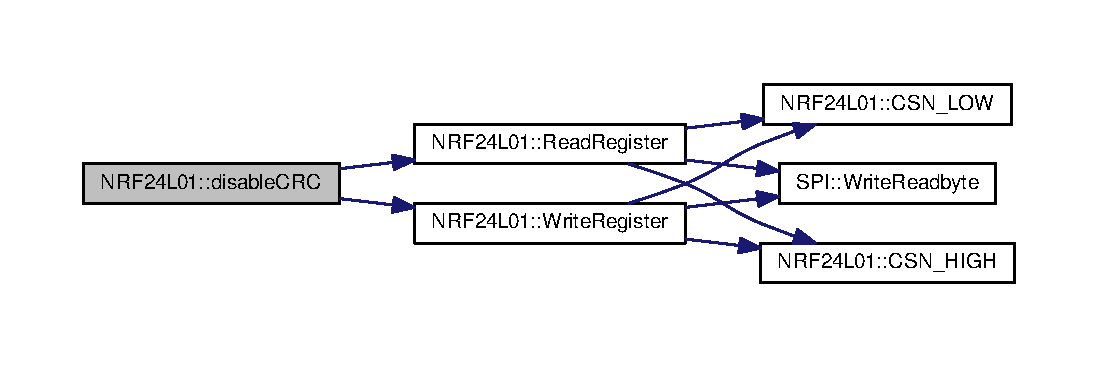
\includegraphics[width=350pt]{classNRF24L01_a1e997f3c946acdbe8bd622e431f80034_cgraph}
\end{center}
\end{figure}


\index{N\+R\+F24\+L01@{N\+R\+F24\+L01}!disable\+Dynamic\+Payloads@{disable\+Dynamic\+Payloads}}
\index{disable\+Dynamic\+Payloads@{disable\+Dynamic\+Payloads}!N\+R\+F24\+L01@{N\+R\+F24\+L01}}
\subsubsection[{\texorpdfstring{disable\+Dynamic\+Payloads(void)}{disableDynamicPayloads(void)}}]{\setlength{\rightskip}{0pt plus 5cm}void N\+R\+F24\+L01\+::disable\+Dynamic\+Payloads (
\begin{DoxyParamCaption}
\item[{void}]{}
\end{DoxyParamCaption}
)}\hypertarget{classNRF24L01_abf6bf0c18b2b12674cfbc150a2bdb778}{}\label{classNRF24L01_abf6bf0c18b2b12674cfbc150a2bdb778}
Disable dynamically-\/sized payloads

This disables dynamic payloads on A\+LL pipes. Since Ack Payloads requires Dynamic Payloads, Ack Payloads are also disabled. If dynamic payloads are later re-\/enabled and ack payloads are desired then \hyperlink{classNRF24L01_ae4067455572c6731211315b3900f5cbd}{enable\+Ack\+Payload()} must be called again as well. 

Here is the call graph for this function\+:\nopagebreak
\begin{figure}[H]
\begin{center}
\leavevmode
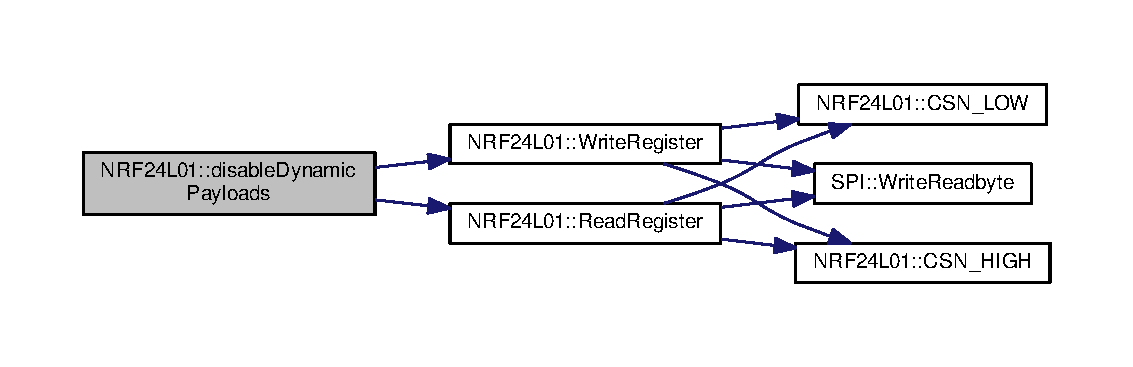
\includegraphics[width=350pt]{classNRF24L01_abf6bf0c18b2b12674cfbc150a2bdb778_cgraph}
\end{center}
\end{figure}


\index{N\+R\+F24\+L01@{N\+R\+F24\+L01}!enable\+Ack\+Payload@{enable\+Ack\+Payload}}
\index{enable\+Ack\+Payload@{enable\+Ack\+Payload}!N\+R\+F24\+L01@{N\+R\+F24\+L01}}
\subsubsection[{\texorpdfstring{enable\+Ack\+Payload(void)}{enableAckPayload(void)}}]{\setlength{\rightskip}{0pt plus 5cm}void N\+R\+F24\+L01\+::enable\+Ack\+Payload (
\begin{DoxyParamCaption}
\item[{void}]{}
\end{DoxyParamCaption}
)}\hypertarget{classNRF24L01_ae4067455572c6731211315b3900f5cbd}{}\label{classNRF24L01_ae4067455572c6731211315b3900f5cbd}
Enable custom payloads on the acknowledge packets

Ack payloads are a handy way to return data back to senders without manually changing the radio modes on both units.

\begin{DoxyNote}{Note}
Ack payloads are dynamic payloads. This only works on pipes 0\&1 by default. Call \hyperlink{classNRF24L01_abd060c4df7efac781ed5812a0ee19d08}{enable\+Dynamic\+Payloads()} to enable on all pipes. 
\end{DoxyNote}


Here is the call graph for this function\+:\nopagebreak
\begin{figure}[H]
\begin{center}
\leavevmode
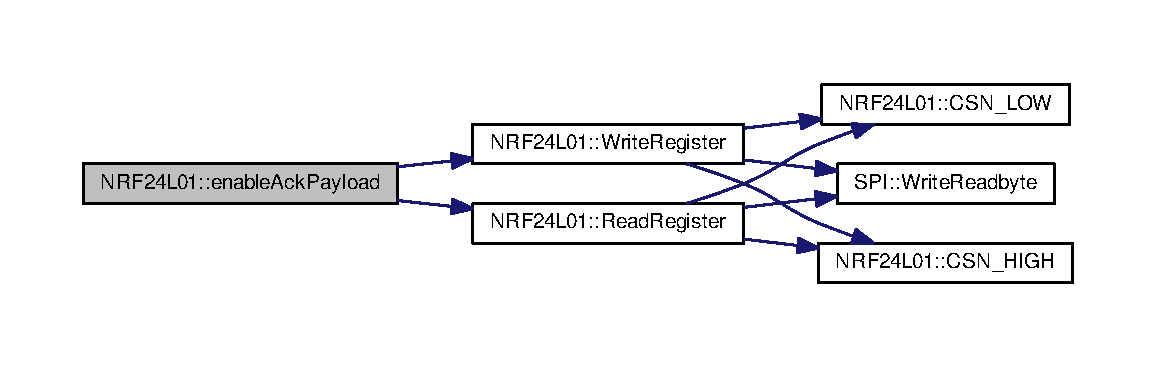
\includegraphics[width=350pt]{classNRF24L01_ae4067455572c6731211315b3900f5cbd_cgraph}
\end{center}
\end{figure}


\index{N\+R\+F24\+L01@{N\+R\+F24\+L01}!enable\+Dynamic\+Ack@{enable\+Dynamic\+Ack}}
\index{enable\+Dynamic\+Ack@{enable\+Dynamic\+Ack}!N\+R\+F24\+L01@{N\+R\+F24\+L01}}
\subsubsection[{\texorpdfstring{enable\+Dynamic\+Ack()}{enableDynamicAck()}}]{\setlength{\rightskip}{0pt plus 5cm}void N\+R\+F24\+L01\+::enable\+Dynamic\+Ack (
\begin{DoxyParamCaption}
\item[{void}]{}
\end{DoxyParamCaption}
)}\hypertarget{classNRF24L01_aeaa968ea74bfd2690fff331e9f115344}{}\label{classNRF24L01_aeaa968ea74bfd2690fff331e9f115344}
Enable dynamic A\+C\+Ks (single write multicast or unicast) for chosen messages

\begin{DoxyNote}{Note}
To enable full multicast or per-\/pipe multicast, use \hyperlink{classNRF24L01_a33b1c7dd1cad95dae57ef87bf3dce5c8}{set\+Auto\+Ack()}
\end{DoxyNote}
\begin{DoxyWarning}{Warning}
This M\+U\+ST be called prior to attempting single write N\+O\+A\+CK calls 
\begin{DoxyCode}
radio.enableDynamicAck();
radio.write(&data,32,1);  \textcolor{comment}{// Sends a payload with no acknowledgement requested}
radio.write(&data,32,0);  \textcolor{comment}{// Sends a payload using auto-retry/autoACK}
\end{DoxyCode}
 
\end{DoxyWarning}


Here is the call graph for this function\+:\nopagebreak
\begin{figure}[H]
\begin{center}
\leavevmode
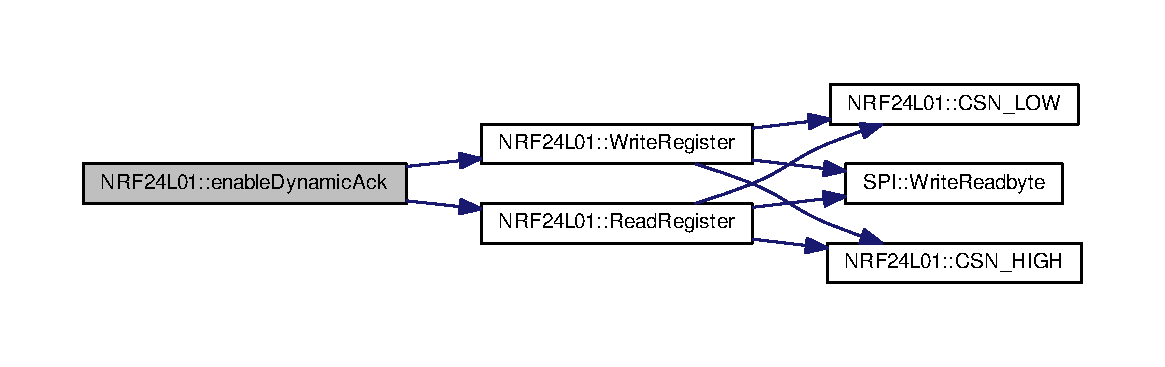
\includegraphics[width=350pt]{classNRF24L01_aeaa968ea74bfd2690fff331e9f115344_cgraph}
\end{center}
\end{figure}


\index{N\+R\+F24\+L01@{N\+R\+F24\+L01}!enable\+Dynamic\+Payloads@{enable\+Dynamic\+Payloads}}
\index{enable\+Dynamic\+Payloads@{enable\+Dynamic\+Payloads}!N\+R\+F24\+L01@{N\+R\+F24\+L01}}
\subsubsection[{\texorpdfstring{enable\+Dynamic\+Payloads(void)}{enableDynamicPayloads(void)}}]{\setlength{\rightskip}{0pt plus 5cm}void N\+R\+F24\+L01\+::enable\+Dynamic\+Payloads (
\begin{DoxyParamCaption}
\item[{void}]{}
\end{DoxyParamCaption}
)}\hypertarget{classNRF24L01_abd060c4df7efac781ed5812a0ee19d08}{}\label{classNRF24L01_abd060c4df7efac781ed5812a0ee19d08}
Enable dynamically-\/sized payloads

This way you don\textquotesingle{}t always have to send large packets just to send them once in a while. This enables dynamic payloads on A\+LL pipes. 

Here is the call graph for this function\+:\nopagebreak
\begin{figure}[H]
\begin{center}
\leavevmode
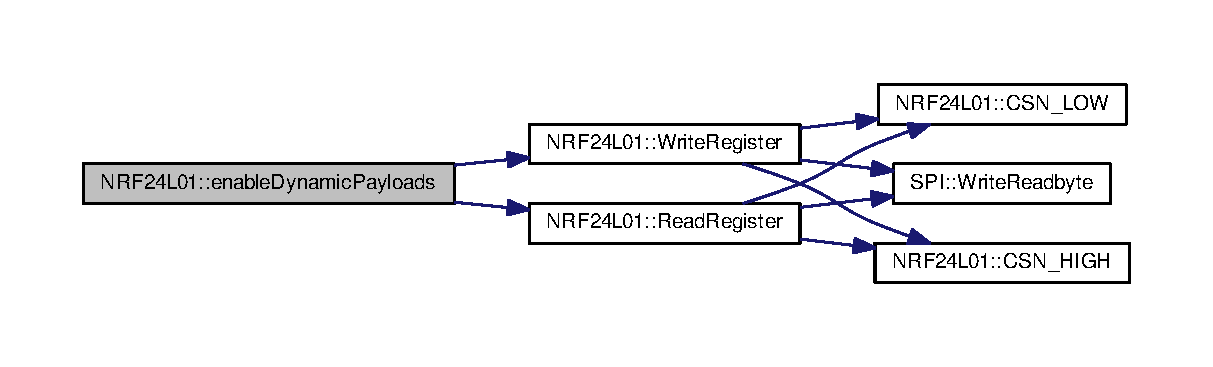
\includegraphics[width=350pt]{classNRF24L01_abd060c4df7efac781ed5812a0ee19d08_cgraph}
\end{center}
\end{figure}


\index{N\+R\+F24\+L01@{N\+R\+F24\+L01}!Flush\+Rx@{Flush\+Rx}}
\index{Flush\+Rx@{Flush\+Rx}!N\+R\+F24\+L01@{N\+R\+F24\+L01}}
\subsubsection[{\texorpdfstring{Flush\+Rx(void)}{FlushRx(void)}}]{\setlength{\rightskip}{0pt plus 5cm}uint8\+\_\+t N\+R\+F24\+L01\+::\+Flush\+Rx (
\begin{DoxyParamCaption}
\item[{void}]{}
\end{DoxyParamCaption}
)\hspace{0.3cm}{\ttfamily [private]}}\hypertarget{classNRF24L01_a83cfc941bafe563f38e183504ee8533c}{}\label{classNRF24L01_a83cfc941bafe563f38e183504ee8533c}
Empty the receive buffer

\begin{DoxyReturn}{Returns}
Current value of status register 
\end{DoxyReturn}


Here is the call graph for this function\+:\nopagebreak
\begin{figure}[H]
\begin{center}
\leavevmode
\includegraphics[width=350pt]{classNRF24L01_a83cfc941bafe563f38e183504ee8533c_cgraph}
\end{center}
\end{figure}


\index{N\+R\+F24\+L01@{N\+R\+F24\+L01}!Flush\+Tx@{Flush\+Tx}}
\index{Flush\+Tx@{Flush\+Tx}!N\+R\+F24\+L01@{N\+R\+F24\+L01}}
\subsubsection[{\texorpdfstring{Flush\+Tx(void)}{FlushTx(void)}}]{\setlength{\rightskip}{0pt plus 5cm}uint8\+\_\+t N\+R\+F24\+L01\+::\+Flush\+Tx (
\begin{DoxyParamCaption}
\item[{void}]{}
\end{DoxyParamCaption}
)}\hypertarget{classNRF24L01_ab40eeb5ca2337c5f15992f29ee3b5b18}{}\label{classNRF24L01_ab40eeb5ca2337c5f15992f29ee3b5b18}
Empty the transmit buffer. This is generally not required in standard operation. May be required in specific cases after \hyperlink{classNRF24L01_a6ad13189b732f237ac148c659ddf6b01}{stop\+Listening()} , if operating at 250\+K\+B\+PS data rate.

\begin{DoxyReturn}{Returns}
Current value of status register 
\end{DoxyReturn}


Here is the call graph for this function\+:\nopagebreak
\begin{figure}[H]
\begin{center}
\leavevmode
\includegraphics[width=350pt]{classNRF24L01_ab40eeb5ca2337c5f15992f29ee3b5b18_cgraph}
\end{center}
\end{figure}


\index{N\+R\+F24\+L01@{N\+R\+F24\+L01}!get\+Channel@{get\+Channel}}
\index{get\+Channel@{get\+Channel}!N\+R\+F24\+L01@{N\+R\+F24\+L01}}
\subsubsection[{\texorpdfstring{get\+Channel(void)}{getChannel(void)}}]{\setlength{\rightskip}{0pt plus 5cm}uint8\+\_\+t N\+R\+F24\+L01\+::get\+Channel (
\begin{DoxyParamCaption}
\item[{void}]{}
\end{DoxyParamCaption}
)}\hypertarget{classNRF24L01_a6b269b519d57d54d0682a29ce9036b12}{}\label{classNRF24L01_a6b269b519d57d54d0682a29ce9036b12}
Get RF communication channel

\begin{DoxyReturn}{Returns}
The currently configured RF Channel 
\end{DoxyReturn}


Here is the call graph for this function\+:\nopagebreak
\begin{figure}[H]
\begin{center}
\leavevmode
\includegraphics[width=350pt]{classNRF24L01_a6b269b519d57d54d0682a29ce9036b12_cgraph}
\end{center}
\end{figure}


\index{N\+R\+F24\+L01@{N\+R\+F24\+L01}!get\+C\+R\+C\+Length@{get\+C\+R\+C\+Length}}
\index{get\+C\+R\+C\+Length@{get\+C\+R\+C\+Length}!N\+R\+F24\+L01@{N\+R\+F24\+L01}}
\subsubsection[{\texorpdfstring{get\+C\+R\+C\+Length(void)}{getCRCLength(void)}}]{\setlength{\rightskip}{0pt plus 5cm}{\bf rf24\+\_\+crclength\+\_\+e} N\+R\+F24\+L01\+::get\+C\+R\+C\+Length (
\begin{DoxyParamCaption}
\item[{void}]{}
\end{DoxyParamCaption}
)}\hypertarget{classNRF24L01_ac83fb86df156475aeda2ef637078fcd3}{}\label{classNRF24L01_ac83fb86df156475aeda2ef637078fcd3}
Get the C\+RC length ~\newline
C\+RC checking cannot be disabled if auto-\/ack is enabled \begin{DoxyReturn}{Returns}
R\+F24\+\_\+\+C\+R\+C\+\_\+\+D\+I\+S\+A\+B\+L\+ED if disabled or R\+F24\+\_\+\+C\+R\+C\+\_\+8 for 8-\/bit or R\+F24\+\_\+\+C\+R\+C\+\_\+16 for 16-\/bit 
\end{DoxyReturn}


Here is the call graph for this function\+:\nopagebreak
\begin{figure}[H]
\begin{center}
\leavevmode
\includegraphics[width=350pt]{classNRF24L01_ac83fb86df156475aeda2ef637078fcd3_cgraph}
\end{center}
\end{figure}


\index{N\+R\+F24\+L01@{N\+R\+F24\+L01}!get\+Data\+Rate@{get\+Data\+Rate}}
\index{get\+Data\+Rate@{get\+Data\+Rate}!N\+R\+F24\+L01@{N\+R\+F24\+L01}}
\subsubsection[{\texorpdfstring{get\+Data\+Rate(void)}{getDataRate(void)}}]{\setlength{\rightskip}{0pt plus 5cm}{\bf rf24\+\_\+datarate\+\_\+e} N\+R\+F24\+L01\+::get\+Data\+Rate (
\begin{DoxyParamCaption}
\item[{void}]{}
\end{DoxyParamCaption}
)}\hypertarget{classNRF24L01_a6184de85c94400cde96b7f83b316efa8}{}\label{classNRF24L01_a6184de85c94400cde96b7f83b316efa8}
Fetches the transmission data rate

\begin{DoxyReturn}{Returns}
Returns the hardware\textquotesingle{}s currently configured datarate. The value is one of 250kbs, R\+F24\+\_\+1\+M\+B\+PS for 1\+Mbps, or R\+F24\+\_\+2\+M\+B\+PS, as defined in the rf24\+\_\+datarate\+\_\+e enum. 
\end{DoxyReturn}


Here is the call graph for this function\+:\nopagebreak
\begin{figure}[H]
\begin{center}
\leavevmode
\includegraphics[width=350pt]{classNRF24L01_a6184de85c94400cde96b7f83b316efa8_cgraph}
\end{center}
\end{figure}


\index{N\+R\+F24\+L01@{N\+R\+F24\+L01}!get\+Dynamic\+Payload\+Size@{get\+Dynamic\+Payload\+Size}}
\index{get\+Dynamic\+Payload\+Size@{get\+Dynamic\+Payload\+Size}!N\+R\+F24\+L01@{N\+R\+F24\+L01}}
\subsubsection[{\texorpdfstring{get\+Dynamic\+Payload\+Size(void)}{getDynamicPayloadSize(void)}}]{\setlength{\rightskip}{0pt plus 5cm}uint8\+\_\+t N\+R\+F24\+L01\+::get\+Dynamic\+Payload\+Size (
\begin{DoxyParamCaption}
\item[{void}]{}
\end{DoxyParamCaption}
)}\hypertarget{classNRF24L01_a0d0cd5dd09d60e06280f378166725d64}{}\label{classNRF24L01_a0d0cd5dd09d60e06280f378166725d64}
Get Dynamic Payload Size

For dynamic payloads, this pulls the size of the payload off the chip

\begin{DoxyNote}{Note}
Corrupt packets are now detected and flushed per the manufacturer. 
\begin{DoxyCode}
\textcolor{keywordflow}{if}(radio.available())\{
  \textcolor{keywordflow}{if}(radio.getDynamicPayloadSize() < 1)\{
    \textcolor{comment}{// Corrupt payload has been flushed}
    \textcolor{keywordflow}{return};
  \}
  radio.read(&data,\textcolor{keyword}{sizeof}(data));
\}
\end{DoxyCode}

\end{DoxyNote}
\begin{DoxyReturn}{Returns}
Payload length of last-\/received dynamic payload 
\end{DoxyReturn}


Here is the call graph for this function\+:\nopagebreak
\begin{figure}[H]
\begin{center}
\leavevmode
\includegraphics[width=350pt]{classNRF24L01_a0d0cd5dd09d60e06280f378166725d64_cgraph}
\end{center}
\end{figure}


\index{N\+R\+F24\+L01@{N\+R\+F24\+L01}!get\+P\+A\+Level@{get\+P\+A\+Level}}
\index{get\+P\+A\+Level@{get\+P\+A\+Level}!N\+R\+F24\+L01@{N\+R\+F24\+L01}}
\subsubsection[{\texorpdfstring{get\+P\+A\+Level(void)}{getPALevel(void)}}]{\setlength{\rightskip}{0pt plus 5cm}uint8\+\_\+t N\+R\+F24\+L01\+::get\+P\+A\+Level (
\begin{DoxyParamCaption}
\item[{void}]{}
\end{DoxyParamCaption}
)}\hypertarget{classNRF24L01_a8fdb80b79100186afad90d9a2a5c79fb}{}\label{classNRF24L01_a8fdb80b79100186afad90d9a2a5c79fb}
Fetches the current PA level.

\hyperlink{classNRF24L01}{N\+R\+F24\+L01}\+: -\/18d\+Bm, -\/12d\+Bm, -\/6d\+Bm and 0d\+Bm S\+I24\+R1\+: -\/6d\+Bm, 0d\+Bm, 3d\+Bm, 7d\+Bm

\begin{DoxyReturn}{Returns}
Returns values 0 to 3 representing the PA Level. 
\end{DoxyReturn}


Here is the call graph for this function\+:\nopagebreak
\begin{figure}[H]
\begin{center}
\leavevmode
\includegraphics[width=350pt]{classNRF24L01_a8fdb80b79100186afad90d9a2a5c79fb_cgraph}
\end{center}
\end{figure}


\index{N\+R\+F24\+L01@{N\+R\+F24\+L01}!get\+Payload\+Size@{get\+Payload\+Size}}
\index{get\+Payload\+Size@{get\+Payload\+Size}!N\+R\+F24\+L01@{N\+R\+F24\+L01}}
\subsubsection[{\texorpdfstring{get\+Payload\+Size(void)}{getPayloadSize(void)}}]{\setlength{\rightskip}{0pt plus 5cm}uint8\+\_\+t N\+R\+F24\+L01\+::get\+Payload\+Size (
\begin{DoxyParamCaption}
\item[{void}]{}
\end{DoxyParamCaption}
)}\hypertarget{classNRF24L01_a4a7f48ca92e14baabd8be1c0831e8c2f}{}\label{classNRF24L01_a4a7f48ca92e14baabd8be1c0831e8c2f}
Get Static Payload Size

\begin{DoxySeeAlso}{See also}
\hyperlink{classNRF24L01_abe5983a57d0d3bd77508e5345774c890}{set\+Payload\+Size()}
\end{DoxySeeAlso}
\begin{DoxyReturn}{Returns}
The number of bytes in the payload 
\end{DoxyReturn}
\index{N\+R\+F24\+L01@{N\+R\+F24\+L01}!get\+Status@{get\+Status}}
\index{get\+Status@{get\+Status}!N\+R\+F24\+L01@{N\+R\+F24\+L01}}
\subsubsection[{\texorpdfstring{get\+Status(void)}{getStatus(void)}}]{\setlength{\rightskip}{0pt plus 5cm}uint8\+\_\+t N\+R\+F24\+L01\+::get\+Status (
\begin{DoxyParamCaption}
\item[{void}]{}
\end{DoxyParamCaption}
)\hspace{0.3cm}{\ttfamily [private]}}\hypertarget{classNRF24L01_a95faa729cb8245516e9eb0248c6d9b0f}{}\label{classNRF24L01_a95faa729cb8245516e9eb0248c6d9b0f}
Retrieve the current status of the chip

\begin{DoxyReturn}{Returns}
Current value of status register 
\end{DoxyReturn}


Here is the call graph for this function\+:\nopagebreak
\begin{figure}[H]
\begin{center}
\leavevmode
\includegraphics[width=350pt]{classNRF24L01_a95faa729cb8245516e9eb0248c6d9b0f_cgraph}
\end{center}
\end{figure}


\index{N\+R\+F24\+L01@{N\+R\+F24\+L01}!Init@{Init}}
\index{Init@{Init}!N\+R\+F24\+L01@{N\+R\+F24\+L01}}
\subsubsection[{\texorpdfstring{Init()}{Init()}}]{\setlength{\rightskip}{0pt plus 5cm}bool N\+R\+F24\+L01\+::\+Init (
\begin{DoxyParamCaption}
\item[{void}]{}
\end{DoxyParamCaption}
)}\hypertarget{classNRF24L01_a2973773d1a158e1cfbf52198f248c548}{}\label{classNRF24L01_a2973773d1a158e1cfbf52198f248c548}
Begin operation of the chip

Call this in setup(), before calling any other methods. 
\begin{DoxyCode}
radio.Init() 
\end{DoxyCode}
 

Here is the call graph for this function\+:\nopagebreak
\begin{figure}[H]
\begin{center}
\leavevmode
\includegraphics[width=350pt]{classNRF24L01_a2973773d1a158e1cfbf52198f248c548_cgraph}
\end{center}
\end{figure}


\index{N\+R\+F24\+L01@{N\+R\+F24\+L01}!is\+Ack\+Payload\+Available@{is\+Ack\+Payload\+Available}}
\index{is\+Ack\+Payload\+Available@{is\+Ack\+Payload\+Available}!N\+R\+F24\+L01@{N\+R\+F24\+L01}}
\subsubsection[{\texorpdfstring{is\+Ack\+Payload\+Available(void)}{isAckPayloadAvailable(void)}}]{\setlength{\rightskip}{0pt plus 5cm}bool N\+R\+F24\+L01\+::is\+Ack\+Payload\+Available (
\begin{DoxyParamCaption}
\item[{void}]{}
\end{DoxyParamCaption}
)}\hypertarget{classNRF24L01_a99aae87d62d5097447305d66a0b3281d}{}\label{classNRF24L01_a99aae87d62d5097447305d66a0b3281d}
Determine if an ack payload was received in the most recent call to \hyperlink{classNRF24L01_a719390c69a2e45df08379f17e3289f4c}{write()}. The regular \hyperlink{classNRF24L01_ab368039cf5448f0ff5d489563d530c7b}{available()} can also be used.

Call \hyperlink{classNRF24L01_a60ed6c6e072a1f41ca560546745ec6da}{read()} to retrieve the ack payload.

\begin{DoxyReturn}{Returns}
True if an ack payload is available. 
\end{DoxyReturn}


Here is the call graph for this function\+:\nopagebreak
\begin{figure}[H]
\begin{center}
\leavevmode
\includegraphics[width=350pt]{classNRF24L01_a99aae87d62d5097447305d66a0b3281d_cgraph}
\end{center}
\end{figure}


\index{N\+R\+F24\+L01@{N\+R\+F24\+L01}!is\+P\+Variant@{is\+P\+Variant}}
\index{is\+P\+Variant@{is\+P\+Variant}!N\+R\+F24\+L01@{N\+R\+F24\+L01}}
\subsubsection[{\texorpdfstring{is\+P\+Variant(void)}{isPVariant(void)}}]{\setlength{\rightskip}{0pt plus 5cm}bool N\+R\+F24\+L01\+::is\+P\+Variant (
\begin{DoxyParamCaption}
\item[{void}]{}
\end{DoxyParamCaption}
)}\hypertarget{classNRF24L01_ad05024c9586c1dc76c2fd95d54ce6b4c}{}\label{classNRF24L01_ad05024c9586c1dc76c2fd95d54ce6b4c}
Determine whether the hardware is an n\+R\+F24\+L01+ or not.

\begin{DoxyReturn}{Returns}
true if the hardware is n\+R\+F24\+L01+ (or compatible) and false if its not. 
\end{DoxyReturn}
\index{N\+R\+F24\+L01@{N\+R\+F24\+L01}!is\+Valid@{is\+Valid}}
\index{is\+Valid@{is\+Valid}!N\+R\+F24\+L01@{N\+R\+F24\+L01}}
\subsubsection[{\texorpdfstring{is\+Valid()}{isValid()}}]{\setlength{\rightskip}{0pt plus 5cm}bool N\+R\+F24\+L01\+::is\+Valid (
\begin{DoxyParamCaption}
{}
\end{DoxyParamCaption}
)\hspace{0.3cm}{\ttfamily [inline]}}\hypertarget{classNRF24L01_aaddabe35ed60f03a2fb2fb475a3cafb5}{}\label{classNRF24L01_aaddabe35ed60f03a2fb2fb475a3cafb5}
Test whether this is a real radio, or a mock shim for debugging. Setting either pin to 0xff is the way to indicate that this is not a real radio.

\begin{DoxyReturn}{Returns}
true if this is a legitimate radio 
\end{DoxyReturn}


Here is the call graph for this function\+:\nopagebreak
\begin{figure}[H]
\begin{center}
\leavevmode
\includegraphics[width=350pt]{classNRF24L01_aaddabe35ed60f03a2fb2fb475a3cafb5_cgraph}
\end{center}
\end{figure}


\index{N\+R\+F24\+L01@{N\+R\+F24\+L01}!mask\+I\+RQ@{mask\+I\+RQ}}
\index{mask\+I\+RQ@{mask\+I\+RQ}!N\+R\+F24\+L01@{N\+R\+F24\+L01}}
\subsubsection[{\texorpdfstring{mask\+I\+R\+Q(bool tx\+\_\+ok, bool tx\+\_\+fail, bool rx\+\_\+ready)}{maskIRQ(bool tx_ok, bool tx_fail, bool rx_ready)}}]{\setlength{\rightskip}{0pt plus 5cm}void N\+R\+F24\+L01\+::mask\+I\+RQ (
\begin{DoxyParamCaption}
\item[{bool}]{tx, }
\item[{bool}]{fail, }
\item[{bool}]{rx}
\end{DoxyParamCaption}
)}\hypertarget{classNRF24L01_ad23d4111c3a26d18db51eb72a5491dbb}{}\label{classNRF24L01_ad23d4111c3a26d18db51eb72a5491dbb}
The radio will generate interrupt signals when a transmission is complete, a transmission fails, or a payload is received. This allows users to mask those interrupts to prevent them from generating a signal on the interrupt pin. Interrupts are enabled on the radio chip by default.


\begin{DoxyCode}
Mask all interrupts except the receive interrupt:

radio.maskIRQ(1,1,0);
\end{DoxyCode}



\begin{DoxyParams}{Parameters}
{\em tx\+\_\+ok} & Mask transmission complete interrupts \\
\hline
{\em tx\+\_\+fail} & Mask transmit failure interrupts \\
\hline
{\em rx\+\_\+ready} & Mask payload received interrupts\\
\hline
\end{DoxyParams}
bool \hyperlink{classNRF24L01_a9351f4bff2196c4f69623f636de7c6a4}{N\+R\+F24\+L01\+::tx\+Stand\+By(uint32\+\_\+t timeout, bool start\+Tx)}\{ \begin{DoxyVerb}if(startTx){
  stopListening();
  CE_HIGH();
}
uint32_t start = millis();

while( ! (ReadRegister(NRF24L01_REG_FIFO_STATUS) & _BV(NRF24L01_REG_TX_EMPTY)) ){
    if( GetStatus() & _BV(NRF24L01_REG_MAX_RT)){
        WriteRegister(NRF24L01_REG_STATUS,_BV(NRF24L01_REG_MAX_RT) );
        CE_LOW();                                     //Set re-transmit
        CE_HIGH();
            if(millis() - start >= timeout){
                CE_LOW(); FlushTx(); return 0;
            }
    }

}


CE_LOW();                  //Set STANDBY-I mode
return 1;
\end{DoxyVerb}


\} 

Here is the call graph for this function\+:\nopagebreak
\begin{figure}[H]
\begin{center}
\leavevmode
\includegraphics[width=350pt]{classNRF24L01_ad23d4111c3a26d18db51eb72a5491dbb_cgraph}
\end{center}
\end{figure}


\index{N\+R\+F24\+L01@{N\+R\+F24\+L01}!open\+Reading\+Pipe@{open\+Reading\+Pipe}}
\index{open\+Reading\+Pipe@{open\+Reading\+Pipe}!N\+R\+F24\+L01@{N\+R\+F24\+L01}}
\subsubsection[{\texorpdfstring{open\+Reading\+Pipe(uint8\+\_\+t number, const uint8\+\_\+t $\ast$address)}{openReadingPipe(uint8_t number, const uint8_t *address)}}]{\setlength{\rightskip}{0pt plus 5cm}void N\+R\+F24\+L01\+::open\+Reading\+Pipe (
\begin{DoxyParamCaption}
\item[{uint8\+\_\+t}]{number, }
\item[{const uint8\+\_\+t $\ast$}]{address}
\end{DoxyParamCaption}
)}\hypertarget{classNRF24L01_a9b458f77f6ae6c42f330710e703dd847}{}\label{classNRF24L01_a9b458f77f6ae6c42f330710e703dd847}
Open a pipe for reading

Up to 6 pipes can be open for reading at once. Open all the required reading pipes, and then call \hyperlink{classNRF24L01_aaabd39829998b609c0dc317af4f141b2}{start\+Listening()}.

\begin{DoxySeeAlso}{See also}
\hyperlink{classNRF24L01_ad64a887cae746be5ca43cf08445feed9}{open\+Writing\+Pipe} 

\hyperlink{classNRF24L01_a17752733515f67aa9f6ed3daa1ed3d1d}{set\+Address\+Width}
\end{DoxySeeAlso}
\begin{DoxyNote}{Note}
Pipes 0 and 1 will store a full 5-\/byte address. Pipes 2-\/5 will technically only store a single byte, borrowing up to 4 additional bytes from pipe \#1 per the assigned address width. 
\end{DoxyNote}
\begin{DoxyWarning}{Warning}
Pipes 1-\/5 should share the same address, except the first byte. Only the first byte in the array should be unique, e.\+g. 
\begin{DoxyCode}
uint8\_t addresses[][6] = \{\textcolor{stringliteral}{"1Node"},\textcolor{stringliteral}{"2Node"}\};
\hyperlink{classNRF24L01_a9b458f77f6ae6c42f330710e703dd847}{openReadingPipe}(1,addresses[0]);
\hyperlink{classNRF24L01_a9b458f77f6ae6c42f330710e703dd847}{openReadingPipe}(2,addresses[1]);
\end{DoxyCode}


Pipe 0 is also used by the writing pipe. So if you open pipe 0 for reading, and then \hyperlink{classNRF24L01_aaabd39829998b609c0dc317af4f141b2}{start\+Listening()}, it will overwrite the writing pipe. Ergo, do an \hyperlink{classNRF24L01_ad64a887cae746be5ca43cf08445feed9}{open\+Writing\+Pipe()} again before \hyperlink{classNRF24L01_a719390c69a2e45df08379f17e3289f4c}{write()}.
\end{DoxyWarning}

\begin{DoxyParams}{Parameters}
{\em number} & Which pipe\# to open, 0-\/5. \\
\hline
{\em address} & The 24, 32 or 40 bit address of the pipe to open. \\
\hline
\end{DoxyParams}


Here is the call graph for this function\+:\nopagebreak
\begin{figure}[H]
\begin{center}
\leavevmode
\includegraphics[width=350pt]{classNRF24L01_a9b458f77f6ae6c42f330710e703dd847_cgraph}
\end{center}
\end{figure}


\index{N\+R\+F24\+L01@{N\+R\+F24\+L01}!open\+Reading\+Pipe@{open\+Reading\+Pipe}}
\index{open\+Reading\+Pipe@{open\+Reading\+Pipe}!N\+R\+F24\+L01@{N\+R\+F24\+L01}}
\subsubsection[{\texorpdfstring{open\+Reading\+Pipe(uint8\+\_\+t number, uint64\+\_\+t address)}{openReadingPipe(uint8_t number, uint64_t address)}}]{\setlength{\rightskip}{0pt plus 5cm}void N\+R\+F24\+L01\+::open\+Reading\+Pipe (
\begin{DoxyParamCaption}
\item[{uint8\+\_\+t}]{number, }
\item[{uint64\+\_\+t}]{address}
\end{DoxyParamCaption}
)}\hypertarget{classNRF24L01_a02c91592a6c762c1a4e86252f8958bd6}{}\label{classNRF24L01_a02c91592a6c762c1a4e86252f8958bd6}
Open a pipe for reading \begin{DoxyNote}{Note}
For compatibility with old code only, see new function
\end{DoxyNote}
\begin{DoxyWarning}{Warning}
Pipes 1-\/5 should share the first 32 bits. Only the least significant byte should be unique, e.\+g. 
\begin{DoxyCode}
\hyperlink{classNRF24L01_a9b458f77f6ae6c42f330710e703dd847}{openReadingPipe}(1,0xF0F0F0F0AA);
\hyperlink{classNRF24L01_a9b458f77f6ae6c42f330710e703dd847}{openReadingPipe}(2,0xF0F0F0F066);
\end{DoxyCode}


Pipe 0 is also used by the writing pipe. So if you open pipe 0 for reading, and then \hyperlink{classNRF24L01_aaabd39829998b609c0dc317af4f141b2}{start\+Listening()}, it will overwrite the writing pipe. Ergo, do an \hyperlink{classNRF24L01_ad64a887cae746be5ca43cf08445feed9}{open\+Writing\+Pipe()} again before \hyperlink{classNRF24L01_a719390c69a2e45df08379f17e3289f4c}{write()}.
\end{DoxyWarning}

\begin{DoxyParams}{Parameters}
{\em number} & Which pipe\# to open, 0-\/5. \\
\hline
{\em address} & The 40-\/bit address of the pipe to open. \\
\hline
\end{DoxyParams}


Here is the call graph for this function\+:\nopagebreak
\begin{figure}[H]
\begin{center}
\leavevmode
\includegraphics[width=350pt]{classNRF24L01_a02c91592a6c762c1a4e86252f8958bd6_cgraph}
\end{center}
\end{figure}


\index{N\+R\+F24\+L01@{N\+R\+F24\+L01}!open\+Writing\+Pipe@{open\+Writing\+Pipe}}
\index{open\+Writing\+Pipe@{open\+Writing\+Pipe}!N\+R\+F24\+L01@{N\+R\+F24\+L01}}
\subsubsection[{\texorpdfstring{open\+Writing\+Pipe(const uint8\+\_\+t $\ast$address)}{openWritingPipe(const uint8_t *address)}}]{\setlength{\rightskip}{0pt plus 5cm}void N\+R\+F24\+L01\+::open\+Writing\+Pipe (
\begin{DoxyParamCaption}
\item[{const uint8\+\_\+t $\ast$}]{address}
\end{DoxyParamCaption}
)}\hypertarget{classNRF24L01_ad64a887cae746be5ca43cf08445feed9}{}\label{classNRF24L01_ad64a887cae746be5ca43cf08445feed9}
New\+: Open a pipe for writing via byte array. Old addressing format retained for compatibility.

Only one writing pipe can be open at once, but you can change the address you\textquotesingle{}ll write to. Call \hyperlink{classNRF24L01_a6ad13189b732f237ac148c659ddf6b01}{stop\+Listening()} first.

Addresses are assigned via a byte array, default is 5 byte address lengths


\begin{DoxyCode}
uint8\_t addresses[][6] = \{\textcolor{stringliteral}{"1Node"},\textcolor{stringliteral}{"2Node"}\};
radio.openWritingPipe(addresses[0]);
\end{DoxyCode}
 
\begin{DoxyCode}
uint8\_t address[] = \{ 0xCC,0xCE,0xCC,0xCE,0xCC \};
radio.openWritingPipe(address);
address[0] = 0x33;
radio.openReadingPipe(1,address);
\end{DoxyCode}
 \begin{DoxySeeAlso}{See also}
\hyperlink{classNRF24L01_a17752733515f67aa9f6ed3daa1ed3d1d}{set\+Address\+Width}
\end{DoxySeeAlso}

\begin{DoxyParams}{Parameters}
{\em address} & The address of the pipe to open. Coordinate these pipe addresses amongst nodes on the network. \\
\hline
\end{DoxyParams}


Here is the call graph for this function\+:\nopagebreak
\begin{figure}[H]
\begin{center}
\leavevmode
\includegraphics[width=350pt]{classNRF24L01_ad64a887cae746be5ca43cf08445feed9_cgraph}
\end{center}
\end{figure}


\index{N\+R\+F24\+L01@{N\+R\+F24\+L01}!open\+Writing\+Pipe@{open\+Writing\+Pipe}}
\index{open\+Writing\+Pipe@{open\+Writing\+Pipe}!N\+R\+F24\+L01@{N\+R\+F24\+L01}}
\subsubsection[{\texorpdfstring{open\+Writing\+Pipe(uint64\+\_\+t address)}{openWritingPipe(uint64_t address)}}]{\setlength{\rightskip}{0pt plus 5cm}void N\+R\+F24\+L01\+::open\+Writing\+Pipe (
\begin{DoxyParamCaption}
\item[{uint64\+\_\+t}]{address}
\end{DoxyParamCaption}
)}\hypertarget{classNRF24L01_a0fe37f8ff95b7c562ad1fc277890e29a}{}\label{classNRF24L01_a0fe37f8ff95b7c562ad1fc277890e29a}
Open a pipe for writing \begin{DoxyNote}{Note}
For compatibility with old code only, see new function
\end{DoxyNote}
Addresses are 40-\/bit hex values, e.\+g.\+:


\begin{DoxyCode}
\hyperlink{classNRF24L01_ad64a887cae746be5ca43cf08445feed9}{openWritingPipe}(0xF0F0F0F0F0);
\end{DoxyCode}



\begin{DoxyParams}{Parameters}
{\em address} & The 40-\/bit address of the pipe to open. \\
\hline
\end{DoxyParams}


Here is the call graph for this function\+:\nopagebreak
\begin{figure}[H]
\begin{center}
\leavevmode
\includegraphics[width=350pt]{classNRF24L01_a0fe37f8ff95b7c562ad1fc277890e29a_cgraph}
\end{center}
\end{figure}


\index{N\+R\+F24\+L01@{N\+R\+F24\+L01}!power\+Down@{power\+Down}}
\index{power\+Down@{power\+Down}!N\+R\+F24\+L01@{N\+R\+F24\+L01}}
\subsubsection[{\texorpdfstring{power\+Down(void)}{powerDown(void)}}]{\setlength{\rightskip}{0pt plus 5cm}void N\+R\+F24\+L01\+::power\+Down (
\begin{DoxyParamCaption}
\item[{void}]{}
\end{DoxyParamCaption}
)}\hypertarget{classNRF24L01_abaf0ed9cb5b24890631d7b8bc0e3cd82}{}\label{classNRF24L01_abaf0ed9cb5b24890631d7b8bc0e3cd82}
Enter low-\/power mode

To return to normal power mode, call \hyperlink{classNRF24L01_a8e184a0a6ca30fbae69c1331a567deda}{power\+Up()}.

\begin{DoxyNote}{Note}
After calling \hyperlink{classNRF24L01_aaabd39829998b609c0dc317af4f141b2}{start\+Listening()}, a basic radio will consume about 13.\+5mA at max PA level. During active transmission, the radio will consume about 11.\+5mA, but this will be reduced to 26uA (.026mA) between sending. In full power\+Down mode, the radio will consume approximately 900nA (.0009mA)
\end{DoxyNote}

\begin{DoxyCode}
radio.powerDown();
avr\_enter\_sleep\_mode(); \textcolor{comment}{// Custom function to sleep the device}
radio.powerUp();
\end{DoxyCode}
 

Here is the call graph for this function\+:\nopagebreak
\begin{figure}[H]
\begin{center}
\leavevmode
\includegraphics[width=350pt]{classNRF24L01_abaf0ed9cb5b24890631d7b8bc0e3cd82_cgraph}
\end{center}
\end{figure}


\index{N\+R\+F24\+L01@{N\+R\+F24\+L01}!power\+Up@{power\+Up}}
\index{power\+Up@{power\+Up}!N\+R\+F24\+L01@{N\+R\+F24\+L01}}
\subsubsection[{\texorpdfstring{power\+Up(void)}{powerUp(void)}}]{\setlength{\rightskip}{0pt plus 5cm}void N\+R\+F24\+L01\+::power\+Up (
\begin{DoxyParamCaption}
\item[{void}]{}
\end{DoxyParamCaption}
)}\hypertarget{classNRF24L01_a8e184a0a6ca30fbae69c1331a567deda}{}\label{classNRF24L01_a8e184a0a6ca30fbae69c1331a567deda}
Leave low-\/power mode -\/ required for normal radio operation after calling \hyperlink{classNRF24L01_abaf0ed9cb5b24890631d7b8bc0e3cd82}{power\+Down()}

To return to low power mode, call \hyperlink{classNRF24L01_abaf0ed9cb5b24890631d7b8bc0e3cd82}{power\+Down()}. \begin{DoxyNote}{Note}
This will take up to 5ms for maximum compatibility 
\end{DoxyNote}


Here is the call graph for this function\+:\nopagebreak
\begin{figure}[H]
\begin{center}
\leavevmode
\includegraphics[width=350pt]{classNRF24L01_a8e184a0a6ca30fbae69c1331a567deda_cgraph}
\end{center}
\end{figure}


\index{N\+R\+F24\+L01@{N\+R\+F24\+L01}!print\+Details@{print\+Details}}
\index{print\+Details@{print\+Details}!N\+R\+F24\+L01@{N\+R\+F24\+L01}}
\subsubsection[{\texorpdfstring{print\+Details(void)}{printDetails(void)}}]{\setlength{\rightskip}{0pt plus 5cm}void N\+R\+F24\+L01\+::print\+Details (
\begin{DoxyParamCaption}
\item[{void}]{}
\end{DoxyParamCaption}
)}\hypertarget{classNRF24L01_ae5c878a568b54ba045a99b9de377b13b}{}\label{classNRF24L01_ae5c878a568b54ba045a99b9de377b13b}
Print a giant block of debugging information to stdout

\begin{DoxyWarning}{Warning}
Does nothing if stdout is not defined. See fdevopen in stdio.\+h The printf.\+h file is included with the library for Arduino. 
\begin{DoxyCode}
\textcolor{preprocessor}{#include <printf.h>}
setup()\{
 Serial.begin(115200);
 printf\_begin();
 ...
\}
\end{DoxyCode}
 
\end{DoxyWarning}
\index{N\+R\+F24\+L01@{N\+R\+F24\+L01}!read@{read}}
\index{read@{read}!N\+R\+F24\+L01@{N\+R\+F24\+L01}}
\subsubsection[{\texorpdfstring{read(void $\ast$buf, uint8\+\_\+t len)}{read(void *buf, uint8_t len)}}]{\setlength{\rightskip}{0pt plus 5cm}void N\+R\+F24\+L01\+::read (
\begin{DoxyParamCaption}
\item[{void $\ast$}]{buf, }
\item[{uint8\+\_\+t}]{len}
\end{DoxyParamCaption}
)}\hypertarget{classNRF24L01_a60ed6c6e072a1f41ca560546745ec6da}{}\label{classNRF24L01_a60ed6c6e072a1f41ca560546745ec6da}
Read the available payload

The size of data read is the fixed payload size, see \hyperlink{classNRF24L01_a4a7f48ca92e14baabd8be1c0831e8c2f}{get\+Payload\+Size()} 
\begin{DoxyParams}{Parameters}
{\em buf} & Pointer to a buffer where the data should be written \\
\hline
{\em len} & Maximum number of bytes to read into the buffer\\
\hline
\end{DoxyParams}

\begin{DoxyCode}
\textcolor{keywordflow}{if}(radio.available())\{
  radio.read(&data,\textcolor{keyword}{sizeof}(data));
\}
\end{DoxyCode}
 \begin{DoxyReturn}{Returns}
No return value. Use \hyperlink{classNRF24L01_ab368039cf5448f0ff5d489563d530c7b}{available()}. 
\end{DoxyReturn}


Here is the call graph for this function\+:\nopagebreak
\begin{figure}[H]
\begin{center}
\leavevmode
\includegraphics[width=350pt]{classNRF24L01_a60ed6c6e072a1f41ca560546745ec6da_cgraph}
\end{center}
\end{figure}


\index{N\+R\+F24\+L01@{N\+R\+F24\+L01}!Read\+Payload@{Read\+Payload}}
\index{Read\+Payload@{Read\+Payload}!N\+R\+F24\+L01@{N\+R\+F24\+L01}}
\subsubsection[{\texorpdfstring{Read\+Payload(void $\ast$buf, uint8\+\_\+t len)}{ReadPayload(void *buf, uint8_t len)}}]{\setlength{\rightskip}{0pt plus 5cm}uint8\+\_\+t N\+R\+F24\+L01\+::\+Read\+Payload (
\begin{DoxyParamCaption}
\item[{void $\ast$}]{buf, }
\item[{uint8\+\_\+t}]{len}
\end{DoxyParamCaption}
)\hspace{0.3cm}{\ttfamily [private]}}\hypertarget{classNRF24L01_ad733911b261f73964817dad526745716}{}\label{classNRF24L01_ad733911b261f73964817dad526745716}
Read the receive payload

The size of data read is the fixed payload size, see \hyperlink{classNRF24L01_a4a7f48ca92e14baabd8be1c0831e8c2f}{get\+Payload\+Size()}


\begin{DoxyParams}{Parameters}
{\em buf} & Where to put the data \\
\hline
{\em len} & Maximum number of bytes to read \\
\hline
\end{DoxyParams}
\begin{DoxyReturn}{Returns}
Current value of status register 
\end{DoxyReturn}


Here is the call graph for this function\+:\nopagebreak
\begin{figure}[H]
\begin{center}
\leavevmode
\includegraphics[width=350pt]{classNRF24L01_ad733911b261f73964817dad526745716_cgraph}
\end{center}
\end{figure}


\index{N\+R\+F24\+L01@{N\+R\+F24\+L01}!Read\+Register@{Read\+Register}}
\index{Read\+Register@{Read\+Register}!N\+R\+F24\+L01@{N\+R\+F24\+L01}}
\subsubsection[{\texorpdfstring{Read\+Register(uint8\+\_\+t reg)}{ReadRegister(uint8_t reg)}}]{\setlength{\rightskip}{0pt plus 5cm}uint8\+\_\+t N\+R\+F24\+L01\+::\+Read\+Register (
\begin{DoxyParamCaption}
\item[{uint8\+\_\+t}]{reg}
\end{DoxyParamCaption}
)\hspace{0.3cm}{\ttfamily [private]}}\hypertarget{classNRF24L01_a6fc7da02296e9f91908e89438ba67901}{}\label{classNRF24L01_a6fc7da02296e9f91908e89438ba67901}
Read single byte from a register


\begin{DoxyParams}{Parameters}
{\em reg} & Which register. Use constants from n\+R\+F24\+L01.\+h \\
\hline
\end{DoxyParams}
\begin{DoxyReturn}{Returns}
Current value of register {\ttfamily reg} 
\end{DoxyReturn}


Here is the call graph for this function\+:\nopagebreak
\begin{figure}[H]
\begin{center}
\leavevmode
\includegraphics[width=350pt]{classNRF24L01_a6fc7da02296e9f91908e89438ba67901_cgraph}
\end{center}
\end{figure}


\index{N\+R\+F24\+L01@{N\+R\+F24\+L01}!Read\+Registers@{Read\+Registers}}
\index{Read\+Registers@{Read\+Registers}!N\+R\+F24\+L01@{N\+R\+F24\+L01}}
\subsubsection[{\texorpdfstring{Read\+Registers(uint8\+\_\+t reg, uint8\+\_\+t $\ast$buf, uint8\+\_\+t len)}{ReadRegisters(uint8_t reg, uint8_t *buf, uint8_t len)}}]{\setlength{\rightskip}{0pt plus 5cm}uint8\+\_\+t N\+R\+F24\+L01\+::\+Read\+Registers (
\begin{DoxyParamCaption}
\item[{uint8\+\_\+t}]{reg, }
\item[{uint8\+\_\+t $\ast$}]{buf, }
\item[{uint8\+\_\+t}]{len}
\end{DoxyParamCaption}
)\hspace{0.3cm}{\ttfamily [private]}}\hypertarget{classNRF24L01_a9766146f8b6bcab59e91e7545484c401}{}\label{classNRF24L01_a9766146f8b6bcab59e91e7545484c401}
Read a chunk of data in from a register


\begin{DoxyParams}{Parameters}
{\em reg} & Which register. Use constants from n\+R\+F24\+L01.\+h \\
\hline
{\em buf} & Where to put the data \\
\hline
{\em len} & How many bytes of data to transfer \\
\hline
\end{DoxyParams}
\begin{DoxyReturn}{Returns}
Current value of status register 
\end{DoxyReturn}


Here is the call graph for this function\+:\nopagebreak
\begin{figure}[H]
\begin{center}
\leavevmode
\includegraphics[width=350pt]{classNRF24L01_a9766146f8b6bcab59e91e7545484c401_cgraph}
\end{center}
\end{figure}


\index{N\+R\+F24\+L01@{N\+R\+F24\+L01}!re\+Use\+TX@{re\+Use\+TX}}
\index{re\+Use\+TX@{re\+Use\+TX}!N\+R\+F24\+L01@{N\+R\+F24\+L01}}
\subsubsection[{\texorpdfstring{re\+Use\+T\+X()}{reUseTX()}}]{\setlength{\rightskip}{0pt plus 5cm}void N\+R\+F24\+L01\+::re\+Use\+TX (
\begin{DoxyParamCaption}
{}
\end{DoxyParamCaption}
)}\hypertarget{classNRF24L01_ad0797d9c6f8ecd9619c9e48168571a01}{}\label{classNRF24L01_ad0797d9c6f8ecd9619c9e48168571a01}
This function is mainly used internally to take advantage of the auto payload re-\/use functionality of the chip, but can be beneficial to users as well.

The function will instruct the radio to re-\/use the data in the F\+I\+FO buffers, and instructs the radio to re-\/send once the timeout limit has been reached. Used by write\+Fast and write\+Blocking to initiate retries when a TX failure occurs. Retries are automatically initiated except with the standard \hyperlink{classNRF24L01_a719390c69a2e45df08379f17e3289f4c}{write()}. This way, data is not flushed from the buffer until switching between modes.

\begin{DoxyNote}{Note}
This is to be used A\+F\+T\+ER auto-\/retry fails if wanting to resend using the built-\/in payload reuse features. After issuing \hyperlink{classNRF24L01_ad0797d9c6f8ecd9619c9e48168571a01}{re\+Use\+T\+X()}, it will keep reending the same payload forever or until a payload is written to the F\+I\+FO, or a flush\+\_\+tx command is given. 
\end{DoxyNote}


Here is the call graph for this function\+:\nopagebreak
\begin{figure}[H]
\begin{center}
\leavevmode
\includegraphics[width=350pt]{classNRF24L01_ad0797d9c6f8ecd9619c9e48168571a01_cgraph}
\end{center}
\end{figure}


\index{N\+R\+F24\+L01@{N\+R\+F24\+L01}!rx\+Fifo\+Full@{rx\+Fifo\+Full}}
\index{rx\+Fifo\+Full@{rx\+Fifo\+Full}!N\+R\+F24\+L01@{N\+R\+F24\+L01}}
\subsubsection[{\texorpdfstring{rx\+Fifo\+Full()}{rxFifoFull()}}]{\setlength{\rightskip}{0pt plus 5cm}bool N\+R\+F24\+L01\+::rx\+Fifo\+Full (
\begin{DoxyParamCaption}
{}
\end{DoxyParamCaption}
)}\hypertarget{classNRF24L01_aebd4d389685333013b4bd12662c0b411}{}\label{classNRF24L01_aebd4d389685333013b4bd12662c0b411}
Check if the radio needs to be read. Can be used to prevent data loss \begin{DoxyReturn}{Returns}
True if all three 32-\/byte radio buffers are full 
\end{DoxyReturn}


Here is the call graph for this function\+:\nopagebreak
\begin{figure}[H]
\begin{center}
\leavevmode
\includegraphics[width=350pt]{classNRF24L01_aebd4d389685333013b4bd12662c0b411_cgraph}
\end{center}
\end{figure}


\index{N\+R\+F24\+L01@{N\+R\+F24\+L01}!set\+Address\+Width@{set\+Address\+Width}}
\index{set\+Address\+Width@{set\+Address\+Width}!N\+R\+F24\+L01@{N\+R\+F24\+L01}}
\subsubsection[{\texorpdfstring{set\+Address\+Width(uint8\+\_\+t a\+\_\+width)}{setAddressWidth(uint8_t a_width)}}]{\setlength{\rightskip}{0pt plus 5cm}void N\+R\+F24\+L01\+::set\+Address\+Width (
\begin{DoxyParamCaption}
\item[{uint8\+\_\+t}]{a\+\_\+width}
\end{DoxyParamCaption}
)}\hypertarget{classNRF24L01_a17752733515f67aa9f6ed3daa1ed3d1d}{}\label{classNRF24L01_a17752733515f67aa9f6ed3daa1ed3d1d}
Set the address width from 3 to 5 bytes (24, 32 or 40 bit)


\begin{DoxyParams}{Parameters}
{\em a\+\_\+width} & The address width to use\+: 3,4 or 5 \\
\hline
\end{DoxyParams}


Here is the call graph for this function\+:\nopagebreak
\begin{figure}[H]
\begin{center}
\leavevmode
\includegraphics[width=350pt]{classNRF24L01_a17752733515f67aa9f6ed3daa1ed3d1d_cgraph}
\end{center}
\end{figure}


\index{N\+R\+F24\+L01@{N\+R\+F24\+L01}!set\+Auto\+Ack@{set\+Auto\+Ack}}
\index{set\+Auto\+Ack@{set\+Auto\+Ack}!N\+R\+F24\+L01@{N\+R\+F24\+L01}}
\subsubsection[{\texorpdfstring{set\+Auto\+Ack(bool enable)}{setAutoAck(bool enable)}}]{\setlength{\rightskip}{0pt plus 5cm}void N\+R\+F24\+L01\+::set\+Auto\+Ack (
\begin{DoxyParamCaption}
\item[{bool}]{enable}
\end{DoxyParamCaption}
)}\hypertarget{classNRF24L01_a33b1c7dd1cad95dae57ef87bf3dce5c8}{}\label{classNRF24L01_a33b1c7dd1cad95dae57ef87bf3dce5c8}
Enable or disable auto-\/acknowlede packets

This is enabled by default, so it\textquotesingle{}s only needed if you want to turn it off for some reason.


\begin{DoxyParams}{Parameters}
{\em enable} & Whether to enable (true) or disable (false) auto-\/acks \\
\hline
\end{DoxyParams}


Here is the call graph for this function\+:\nopagebreak
\begin{figure}[H]
\begin{center}
\leavevmode
\includegraphics[width=350pt]{classNRF24L01_a33b1c7dd1cad95dae57ef87bf3dce5c8_cgraph}
\end{center}
\end{figure}


\index{N\+R\+F24\+L01@{N\+R\+F24\+L01}!set\+Auto\+Ack@{set\+Auto\+Ack}}
\index{set\+Auto\+Ack@{set\+Auto\+Ack}!N\+R\+F24\+L01@{N\+R\+F24\+L01}}
\subsubsection[{\texorpdfstring{set\+Auto\+Ack(uint8\+\_\+t pipe, bool enable)}{setAutoAck(uint8_t pipe, bool enable)}}]{\setlength{\rightskip}{0pt plus 5cm}void N\+R\+F24\+L01\+::set\+Auto\+Ack (
\begin{DoxyParamCaption}
\item[{uint8\+\_\+t}]{pipe, }
\item[{bool}]{enable}
\end{DoxyParamCaption}
)}\hypertarget{classNRF24L01_a79cab6f958c8d9e18273d7c4750480fd}{}\label{classNRF24L01_a79cab6f958c8d9e18273d7c4750480fd}
Enable or disable auto-\/acknowlede packets on a per pipeline basis.

AA is enabled by default, so it\textquotesingle{}s only needed if you want to turn it off/on for some reason on a per pipeline basis.


\begin{DoxyParams}{Parameters}
{\em pipe} & Which pipeline to modify \\
\hline
{\em enable} & Whether to enable (true) or disable (false) auto-\/acks \\
\hline
\end{DoxyParams}


Here is the call graph for this function\+:\nopagebreak
\begin{figure}[H]
\begin{center}
\leavevmode
\includegraphics[width=350pt]{classNRF24L01_a79cab6f958c8d9e18273d7c4750480fd_cgraph}
\end{center}
\end{figure}


\index{N\+R\+F24\+L01@{N\+R\+F24\+L01}!set\+Channel@{set\+Channel}}
\index{set\+Channel@{set\+Channel}!N\+R\+F24\+L01@{N\+R\+F24\+L01}}
\subsubsection[{\texorpdfstring{set\+Channel(uint8\+\_\+t channel)}{setChannel(uint8_t channel)}}]{\setlength{\rightskip}{0pt plus 5cm}void N\+R\+F24\+L01\+::set\+Channel (
\begin{DoxyParamCaption}
\item[{uint8\+\_\+t}]{channel}
\end{DoxyParamCaption}
)}\hypertarget{classNRF24L01_aa8eaf9d5ed604f60a00cd79fed9edad7}{}\label{classNRF24L01_aa8eaf9d5ed604f60a00cd79fed9edad7}
Set RF communication channel


\begin{DoxyParams}{Parameters}
{\em channel} & Which RF channel to communicate on, 0-\/125 \\
\hline
\end{DoxyParams}


Here is the call graph for this function\+:\nopagebreak
\begin{figure}[H]
\begin{center}
\leavevmode
\includegraphics[width=350pt]{classNRF24L01_aa8eaf9d5ed604f60a00cd79fed9edad7_cgraph}
\end{center}
\end{figure}


\index{N\+R\+F24\+L01@{N\+R\+F24\+L01}!set\+C\+R\+C\+Length@{set\+C\+R\+C\+Length}}
\index{set\+C\+R\+C\+Length@{set\+C\+R\+C\+Length}!N\+R\+F24\+L01@{N\+R\+F24\+L01}}
\subsubsection[{\texorpdfstring{set\+C\+R\+C\+Length(uint8\+\_\+t length)}{setCRCLength(uint8_t length)}}]{\setlength{\rightskip}{0pt plus 5cm}void N\+R\+F24\+L01\+::set\+C\+R\+C\+Length (
\begin{DoxyParamCaption}
\item[{uint8\+\_\+t}]{length}
\end{DoxyParamCaption}
)}\hypertarget{classNRF24L01_a6081dd6dd9cdffbc1c7534ee1824201d}{}\label{classNRF24L01_a6081dd6dd9cdffbc1c7534ee1824201d}
Set the C\+RC length ~\newline
C\+RC checking cannot be disabled if auto-\/ack is enabled 
\begin{DoxyParams}{Parameters}
{\em length} & R\+F24\+\_\+\+C\+R\+C\+\_\+8 for 8-\/bit or R\+F24\+\_\+\+C\+R\+C\+\_\+16 for 16-\/bit \\
\hline
\end{DoxyParams}


Here is the call graph for this function\+:\nopagebreak
\begin{figure}[H]
\begin{center}
\leavevmode
\includegraphics[width=350pt]{classNRF24L01_a6081dd6dd9cdffbc1c7534ee1824201d_cgraph}
\end{center}
\end{figure}


\index{N\+R\+F24\+L01@{N\+R\+F24\+L01}!set\+Data\+Rate@{set\+Data\+Rate}}
\index{set\+Data\+Rate@{set\+Data\+Rate}!N\+R\+F24\+L01@{N\+R\+F24\+L01}}
\subsubsection[{\texorpdfstring{set\+Data\+Rate(uint8\+\_\+t speed)}{setDataRate(uint8_t speed)}}]{\setlength{\rightskip}{0pt plus 5cm}bool N\+R\+F24\+L01\+::set\+Data\+Rate (
\begin{DoxyParamCaption}
\item[{uint8\+\_\+t}]{speed}
\end{DoxyParamCaption}
)}\hypertarget{classNRF24L01_a9db0803c6d87e6ada7febea2240a7b1c}{}\label{classNRF24L01_a9db0803c6d87e6ada7febea2240a7b1c}
Set the transmission data rate

\begin{DoxyWarning}{Warning}
setting R\+F24\+\_\+250\+K\+B\+PS will fail for non-\/plus units
\end{DoxyWarning}

\begin{DoxyParams}{Parameters}
{\em speed} & R\+F24\+\_\+250\+K\+B\+PS for 250kbs, R\+F24\+\_\+1\+M\+B\+PS for 1\+Mbps, or R\+F24\+\_\+2\+M\+B\+PS for 2\+Mbps \\
\hline
\end{DoxyParams}
\begin{DoxyReturn}{Returns}
true if the change was successful 
\end{DoxyReturn}


Here is the call graph for this function\+:\nopagebreak
\begin{figure}[H]
\begin{center}
\leavevmode
\includegraphics[width=350pt]{classNRF24L01_a9db0803c6d87e6ada7febea2240a7b1c_cgraph}
\end{center}
\end{figure}


\index{N\+R\+F24\+L01@{N\+R\+F24\+L01}!set\+P\+A\+Level@{set\+P\+A\+Level}}
\index{set\+P\+A\+Level@{set\+P\+A\+Level}!N\+R\+F24\+L01@{N\+R\+F24\+L01}}
\subsubsection[{\texorpdfstring{set\+P\+A\+Level(uint8\+\_\+t level)}{setPALevel(uint8_t level)}}]{\setlength{\rightskip}{0pt plus 5cm}void N\+R\+F24\+L01\+::set\+P\+A\+Level (
\begin{DoxyParamCaption}
\item[{uint8\+\_\+t}]{level}
\end{DoxyParamCaption}
)}\hypertarget{classNRF24L01_a7319961d6048e32546ad5df934bd42d8}{}\label{classNRF24L01_a7319961d6048e32546ad5df934bd42d8}
Set Power Amplifier (PA) level to one of four levels\+: R\+F24\+\_\+\+P\+A\+\_\+\+M\+IN, R\+F24\+\_\+\+P\+A\+\_\+\+L\+OW, R\+F24\+\_\+\+P\+A\+\_\+\+H\+I\+GH and R\+F24\+\_\+\+P\+A\+\_\+\+M\+AX

The power levels correspond to the following output levels respectively\+: \hyperlink{classNRF24L01}{N\+R\+F24\+L01}\+: -\/18d\+Bm, -\/12d\+Bm,-\/6d\+BM, and 0d\+Bm

S\+I24\+R1\+: -\/6d\+Bm, 0d\+Bm, 3d\+BM, and 7d\+Bm.


\begin{DoxyParams}{Parameters}
{\em level} & Desired PA level. \\
\hline
\end{DoxyParams}


Here is the call graph for this function\+:\nopagebreak
\begin{figure}[H]
\begin{center}
\leavevmode
\includegraphics[width=350pt]{classNRF24L01_a7319961d6048e32546ad5df934bd42d8_cgraph}
\end{center}
\end{figure}


\index{N\+R\+F24\+L01@{N\+R\+F24\+L01}!set\+Payload\+Size@{set\+Payload\+Size}}
\index{set\+Payload\+Size@{set\+Payload\+Size}!N\+R\+F24\+L01@{N\+R\+F24\+L01}}
\subsubsection[{\texorpdfstring{set\+Payload\+Size(uint8\+\_\+t size)}{setPayloadSize(uint8_t size)}}]{\setlength{\rightskip}{0pt plus 5cm}void N\+R\+F24\+L01\+::set\+Payload\+Size (
\begin{DoxyParamCaption}
\item[{uint8\+\_\+t}]{size}
\end{DoxyParamCaption}
)}\hypertarget{classNRF24L01_abe5983a57d0d3bd77508e5345774c890}{}\label{classNRF24L01_abe5983a57d0d3bd77508e5345774c890}
Set Static Payload Size

This implementation uses a pre-\/stablished fixed payload size for all transmissions. If this method is never called, the driver will always transmit the maximum payload size (32 bytes), no matter how much was sent to \hyperlink{classNRF24L01_a719390c69a2e45df08379f17e3289f4c}{write()}.

\begin{DoxyRefDesc}{Todo}
\item[\hyperlink{todo__todo000002}{Todo}]Implement variable-\/sized payloads feature\end{DoxyRefDesc}



\begin{DoxyParams}{Parameters}
{\em size} & The number of bytes in the payload \\
\hline
\end{DoxyParams}
\index{N\+R\+F24\+L01@{N\+R\+F24\+L01}!set\+Retries@{set\+Retries}}
\index{set\+Retries@{set\+Retries}!N\+R\+F24\+L01@{N\+R\+F24\+L01}}
\subsubsection[{\texorpdfstring{set\+Retries(uint8\+\_\+t delay, uint8\+\_\+t count)}{setRetries(uint8_t delay, uint8_t count)}}]{\setlength{\rightskip}{0pt plus 5cm}void N\+R\+F24\+L01\+::set\+Retries (
\begin{DoxyParamCaption}
\item[{uint8\+\_\+t}]{delay, }
\item[{uint8\+\_\+t}]{count}
\end{DoxyParamCaption}
)}\hypertarget{classNRF24L01_a0bb209d94b62e2a28af53179af713f3c}{}\label{classNRF24L01_a0bb209d94b62e2a28af53179af713f3c}
Set the number and delay of retries upon failed submit


\begin{DoxyParams}{Parameters}
{\em delay} & How long to wait between each retry, in multiples of 250us, max is 15. 0 means 250us, 15 means 4000us. \\
\hline
{\em count} & How many retries before giving up, max 15 \\
\hline
\end{DoxyParams}


Here is the call graph for this function\+:\nopagebreak
\begin{figure}[H]
\begin{center}
\leavevmode
\includegraphics[width=350pt]{classNRF24L01_a0bb209d94b62e2a28af53179af713f3c_cgraph}
\end{center}
\end{figure}


\index{N\+R\+F24\+L01@{N\+R\+F24\+L01}!spi\+Trans@{spi\+Trans}}
\index{spi\+Trans@{spi\+Trans}!N\+R\+F24\+L01@{N\+R\+F24\+L01}}
\subsubsection[{\texorpdfstring{spi\+Trans(uint8\+\_\+t cmd)}{spiTrans(uint8_t cmd)}}]{\setlength{\rightskip}{0pt plus 5cm}uint8\+\_\+t N\+R\+F24\+L01\+::spi\+Trans (
\begin{DoxyParamCaption}
\item[{uint8\+\_\+t}]{cmd}
\end{DoxyParamCaption}
)\hspace{0.3cm}{\ttfamily [private]}}\hypertarget{classNRF24L01_ab604b1e177e4812e33ebc39287503197}{}\label{classNRF24L01_ab604b1e177e4812e33ebc39287503197}
Built in spi transfer function to simplify repeating code repeating code 

Here is the call graph for this function\+:\nopagebreak
\begin{figure}[H]
\begin{center}
\leavevmode
\includegraphics[width=350pt]{classNRF24L01_ab604b1e177e4812e33ebc39287503197_cgraph}
\end{center}
\end{figure}


\index{N\+R\+F24\+L01@{N\+R\+F24\+L01}!start\+Fast\+Write@{start\+Fast\+Write}}
\index{start\+Fast\+Write@{start\+Fast\+Write}!N\+R\+F24\+L01@{N\+R\+F24\+L01}}
\subsubsection[{\texorpdfstring{start\+Fast\+Write(const void $\ast$buf, uint8\+\_\+t len, const bool multicast, bool start\+Tx=1)}{startFastWrite(const void *buf, uint8_t len, const bool multicast, bool startTx=1)}}]{\setlength{\rightskip}{0pt plus 5cm}void N\+R\+F24\+L01\+::start\+Fast\+Write (
\begin{DoxyParamCaption}
\item[{const void $\ast$}]{buf, }
\item[{uint8\+\_\+t}]{len, }
\item[{const bool}]{multicast, }
\item[{bool}]{start\+Tx = {\ttfamily 1}}
\end{DoxyParamCaption}
)}\hypertarget{classNRF24L01_ab1ca9025a8740bc38ad5dd7a427e2d4f}{}\label{classNRF24L01_ab1ca9025a8740bc38ad5dd7a427e2d4f}
Non-\/blocking write to the open writing pipe used for buffered writes

\begin{DoxyNote}{Note}
Optimization\+: This function now leaves the CE pin high, so the radio will remain in TX or S\+T\+A\+N\+D\+B\+Y-\/\+II Mode until a \hyperlink{classNRF24L01_a4416a731de8d23cac507e8b69ec2becc}{tx\+Stand\+By()} command is issued. Can be used as an alternative to \hyperlink{classNRF24L01_a282e44fa8d6ec7542e9d725cf048f6b2}{start\+Write()} if writing multiple payloads at once. 
\end{DoxyNote}
\begin{DoxyWarning}{Warning}
It is important to never keep the n\+R\+F24\+L01 in TX mode with F\+I\+FO full for more than 4ms at a time. If the auto retransmit/auto\+Ack is enabled, the n\+R\+F24\+L01 is never in TX mode long enough to disobey this rule. Allow the F\+I\+FO to clear by issuing \hyperlink{classNRF24L01_a4416a731de8d23cac507e8b69ec2becc}{tx\+Stand\+By()} or ensure appropriate time between transmissions.
\end{DoxyWarning}
\begin{DoxySeeAlso}{See also}
\hyperlink{classNRF24L01_a719390c69a2e45df08379f17e3289f4c}{write()} 

\hyperlink{classNRF24L01_a693f48de67c8b11ed5860dc481fcfc99}{write\+Fast()} 

\hyperlink{classNRF24L01_a282e44fa8d6ec7542e9d725cf048f6b2}{start\+Write()} 

\hyperlink{classNRF24L01_ac2c2500350c3dde0df4f09111f8f1b84}{write\+Blocking()}
\end{DoxySeeAlso}
For single no\+Ack writes see\+: \begin{DoxySeeAlso}{See also}
\hyperlink{classNRF24L01_aeaa968ea74bfd2690fff331e9f115344}{enable\+Dynamic\+Ack()} 

\hyperlink{classNRF24L01_a33b1c7dd1cad95dae57ef87bf3dce5c8}{set\+Auto\+Ack()}
\end{DoxySeeAlso}

\begin{DoxyParams}{Parameters}
{\em buf} & Pointer to the data to be sent \\
\hline
{\em len} & Number of bytes to be sent \\
\hline
{\em multicast} & Request A\+CK (0) or N\+O\+A\+CK (1) \\
\hline
\end{DoxyParams}
\begin{DoxyReturn}{Returns}
True if the payload was delivered successfully false if not 
\end{DoxyReturn}


Here is the call graph for this function\+:\nopagebreak
\begin{figure}[H]
\begin{center}
\leavevmode
\includegraphics[width=350pt]{classNRF24L01_ab1ca9025a8740bc38ad5dd7a427e2d4f_cgraph}
\end{center}
\end{figure}


\index{N\+R\+F24\+L01@{N\+R\+F24\+L01}!start\+Listening@{start\+Listening}}
\index{start\+Listening@{start\+Listening}!N\+R\+F24\+L01@{N\+R\+F24\+L01}}
\subsubsection[{\texorpdfstring{start\+Listening()}{startListening()}}]{\setlength{\rightskip}{0pt plus 5cm}void N\+R\+F24\+L01\+::start\+Listening (
\begin{DoxyParamCaption}
\item[{void}]{}
\end{DoxyParamCaption}
)}\hypertarget{classNRF24L01_aaabd39829998b609c0dc317af4f141b2}{}\label{classNRF24L01_aaabd39829998b609c0dc317af4f141b2}
Start listening on the pipes opened for reading.


\begin{DoxyEnumerate}
\item Be sure to call \hyperlink{classNRF24L01_a9b458f77f6ae6c42f330710e703dd847}{open\+Reading\+Pipe()} first.
\item Do not call \hyperlink{classNRF24L01_a719390c69a2e45df08379f17e3289f4c}{write()} while in this mode, without first calling \hyperlink{classNRF24L01_a6ad13189b732f237ac148c659ddf6b01}{stop\+Listening()}.
\item Call \hyperlink{classNRF24L01_ab368039cf5448f0ff5d489563d530c7b}{available()} to check for incoming traffic, and \hyperlink{classNRF24L01_a60ed6c6e072a1f41ca560546745ec6da}{read()} to get it.
\end{DoxyEnumerate}


\begin{DoxyCode}
Open reading pipe 1 \textcolor{keyword}{using} address CCCECCCECC

byte address[] = \{ 0xCC,0xCE,0xCC,0xCE,0xCC \};
radio.openReadingPipe(1,address);
radio.startListening();
\end{DoxyCode}
 

Here is the call graph for this function\+:\nopagebreak
\begin{figure}[H]
\begin{center}
\leavevmode
\includegraphics[width=350pt]{classNRF24L01_aaabd39829998b609c0dc317af4f141b2_cgraph}
\end{center}
\end{figure}


\index{N\+R\+F24\+L01@{N\+R\+F24\+L01}!start\+Write@{start\+Write}}
\index{start\+Write@{start\+Write}!N\+R\+F24\+L01@{N\+R\+F24\+L01}}
\subsubsection[{\texorpdfstring{start\+Write(const void $\ast$buf, uint8\+\_\+t len, const bool multicast)}{startWrite(const void *buf, uint8_t len, const bool multicast)}}]{\setlength{\rightskip}{0pt plus 5cm}void N\+R\+F24\+L01\+::start\+Write (
\begin{DoxyParamCaption}
\item[{const void $\ast$}]{buf, }
\item[{uint8\+\_\+t}]{len, }
\item[{const bool}]{multicast}
\end{DoxyParamCaption}
)}\hypertarget{classNRF24L01_a282e44fa8d6ec7542e9d725cf048f6b2}{}\label{classNRF24L01_a282e44fa8d6ec7542e9d725cf048f6b2}
Non-\/blocking write to the open writing pipe

Just like \hyperlink{classNRF24L01_a719390c69a2e45df08379f17e3289f4c}{write()}, but it returns immediately. To find out what happened to the send, catch the I\+RQ and then call \hyperlink{classNRF24L01_ad98d10f3759d41e565397aba824d121b}{what\+Happened()}.

\begin{DoxySeeAlso}{See also}
\hyperlink{classNRF24L01_a719390c69a2e45df08379f17e3289f4c}{write()} 

\hyperlink{classNRF24L01_a693f48de67c8b11ed5860dc481fcfc99}{write\+Fast()} 

\hyperlink{classNRF24L01_ab1ca9025a8740bc38ad5dd7a427e2d4f}{start\+Fast\+Write()} 

\hyperlink{classNRF24L01_ad98d10f3759d41e565397aba824d121b}{what\+Happened()}
\end{DoxySeeAlso}
For single no\+Ack writes see\+: \begin{DoxySeeAlso}{See also}
\hyperlink{classNRF24L01_aeaa968ea74bfd2690fff331e9f115344}{enable\+Dynamic\+Ack()} 

\hyperlink{classNRF24L01_a33b1c7dd1cad95dae57ef87bf3dce5c8}{set\+Auto\+Ack()}
\end{DoxySeeAlso}

\begin{DoxyParams}{Parameters}
{\em buf} & Pointer to the data to be sent \\
\hline
{\em len} & Number of bytes to be sent \\
\hline
{\em multicast} & Request A\+CK (0) or N\+O\+A\+CK (1) \\
\hline
\end{DoxyParams}


Here is the call graph for this function\+:\nopagebreak
\begin{figure}[H]
\begin{center}
\leavevmode
\includegraphics[width=350pt]{classNRF24L01_a282e44fa8d6ec7542e9d725cf048f6b2_cgraph}
\end{center}
\end{figure}


\index{N\+R\+F24\+L01@{N\+R\+F24\+L01}!stop\+Listening@{stop\+Listening}}
\index{stop\+Listening@{stop\+Listening}!N\+R\+F24\+L01@{N\+R\+F24\+L01}}
\subsubsection[{\texorpdfstring{stop\+Listening()}{stopListening()}}]{\setlength{\rightskip}{0pt plus 5cm}void N\+R\+F24\+L01\+::stop\+Listening (
\begin{DoxyParamCaption}
\item[{void}]{}
\end{DoxyParamCaption}
)}\hypertarget{classNRF24L01_a6ad13189b732f237ac148c659ddf6b01}{}\label{classNRF24L01_a6ad13189b732f237ac148c659ddf6b01}
Stop listening for incoming messages, and switch to transmit mode.

Do this before calling \hyperlink{classNRF24L01_a719390c69a2e45df08379f17e3289f4c}{write()}. 
\begin{DoxyCode}
radio.stopListening();
radio.write(&data,\textcolor{keyword}{sizeof}(data));
\end{DoxyCode}
 

Here is the call graph for this function\+:\nopagebreak
\begin{figure}[H]
\begin{center}
\leavevmode
\includegraphics[width=350pt]{classNRF24L01_a6ad13189b732f237ac148c659ddf6b01_cgraph}
\end{center}
\end{figure}


\index{N\+R\+F24\+L01@{N\+R\+F24\+L01}!test\+Carrier@{test\+Carrier}}
\index{test\+Carrier@{test\+Carrier}!N\+R\+F24\+L01@{N\+R\+F24\+L01}}
\subsubsection[{\texorpdfstring{test\+Carrier(void)}{testCarrier(void)}}]{\setlength{\rightskip}{0pt plus 5cm}bool N\+R\+F24\+L01\+::test\+Carrier (
\begin{DoxyParamCaption}
\item[{void}]{}
\end{DoxyParamCaption}
)}\hypertarget{classNRF24L01_a5e934f8f7d37245264ad16e3c360eca7}{}\label{classNRF24L01_a5e934f8f7d37245264ad16e3c360eca7}
Test whether there was a carrier on the line for the previous listening period.

Useful to check for interference on the current channel.

\begin{DoxyReturn}{Returns}
true if was carrier, false if not 
\end{DoxyReturn}


Here is the call graph for this function\+:\nopagebreak
\begin{figure}[H]
\begin{center}
\leavevmode
\includegraphics[width=350pt]{classNRF24L01_a5e934f8f7d37245264ad16e3c360eca7_cgraph}
\end{center}
\end{figure}


\index{N\+R\+F24\+L01@{N\+R\+F24\+L01}!test\+R\+PD@{test\+R\+PD}}
\index{test\+R\+PD@{test\+R\+PD}!N\+R\+F24\+L01@{N\+R\+F24\+L01}}
\subsubsection[{\texorpdfstring{test\+R\+P\+D(void)}{testRPD(void)}}]{\setlength{\rightskip}{0pt plus 5cm}bool N\+R\+F24\+L01\+::test\+R\+PD (
\begin{DoxyParamCaption}
\item[{void}]{}
\end{DoxyParamCaption}
)}\hypertarget{classNRF24L01_abf1d84ed988aa6c7925ebb712b7c7f60}{}\label{classNRF24L01_abf1d84ed988aa6c7925ebb712b7c7f60}
Test whether a signal (carrier or otherwise) greater than or equal to -\/64d\+Bm is present on the channel. Valid only on n\+R\+F24\+L01P (+) hardware. On n\+R\+F24\+L01, use \hyperlink{classNRF24L01_a5e934f8f7d37245264ad16e3c360eca7}{test\+Carrier()}.

Useful to check for interference on the current channel and channel hopping strategies.


\begin{DoxyCode}
\textcolor{keywordtype}{bool} goodSignal = radio.testRPD();
\textcolor{keywordflow}{if}(radio.available())\{
   Serial.println(goodSignal ? \textcolor{stringliteral}{"Strong signal > 64dBm"} : \textcolor{stringliteral}{"Weak signal < 64dBm"} );
   radio.read(0,0);
\}
\end{DoxyCode}
 \begin{DoxyReturn}{Returns}
true if signal =$>$ -\/64d\+Bm, false if not 
\end{DoxyReturn}


Here is the call graph for this function\+:\nopagebreak
\begin{figure}[H]
\begin{center}
\leavevmode
\includegraphics[width=350pt]{classNRF24L01_abf1d84ed988aa6c7925ebb712b7c7f60_cgraph}
\end{center}
\end{figure}


\index{N\+R\+F24\+L01@{N\+R\+F24\+L01}!Toggle\+Features@{Toggle\+Features}}
\index{Toggle\+Features@{Toggle\+Features}!N\+R\+F24\+L01@{N\+R\+F24\+L01}}
\subsubsection[{\texorpdfstring{Toggle\+Features(void)}{ToggleFeatures(void)}}]{\setlength{\rightskip}{0pt plus 5cm}void N\+R\+F24\+L01\+::\+Toggle\+Features (
\begin{DoxyParamCaption}
\item[{void}]{}
\end{DoxyParamCaption}
)\hspace{0.3cm}{\ttfamily [private]}}\hypertarget{classNRF24L01_aceeaa16f91d7c5fd6a429a6adf678bd4}{}\label{classNRF24L01_aceeaa16f91d7c5fd6a429a6adf678bd4}
Turn on or off the special features of the chip

The chip has certain \textquotesingle{}features\textquotesingle{} which are only available when the \textquotesingle{}features\textquotesingle{} are enabled. See the datasheet for details. 

Here is the call graph for this function\+:\nopagebreak
\begin{figure}[H]
\begin{center}
\leavevmode
\includegraphics[width=350pt]{classNRF24L01_aceeaa16f91d7c5fd6a429a6adf678bd4_cgraph}
\end{center}
\end{figure}


\index{N\+R\+F24\+L01@{N\+R\+F24\+L01}!tx\+Stand\+By@{tx\+Stand\+By}}
\index{tx\+Stand\+By@{tx\+Stand\+By}!N\+R\+F24\+L01@{N\+R\+F24\+L01}}
\subsubsection[{\texorpdfstring{tx\+Stand\+By()}{txStandBy()}}]{\setlength{\rightskip}{0pt plus 5cm}bool N\+R\+F24\+L01\+::tx\+Stand\+By (
\begin{DoxyParamCaption}
{}
\end{DoxyParamCaption}
)}\hypertarget{classNRF24L01_a4416a731de8d23cac507e8b69ec2becc}{}\label{classNRF24L01_a4416a731de8d23cac507e8b69ec2becc}
This function should be called as soon as transmission is finished to drop the radio back to S\+T\+A\+N\+D\+B\+Y-\/I mode. If not issued, the radio will remain in S\+T\+A\+N\+D\+B\+Y-\/\+II mode which, per the data sheet, is not a recommended operating mode.

\begin{DoxyNote}{Note}
When transmitting data in rapid succession, it is still recommended by the manufacturer to drop the radio out of TX or S\+T\+A\+N\+D\+B\+Y-\/\+II mode if there is time enough between sends for the F\+I\+F\+Os to empty. This is not required if auto-\/ack is enabled.
\end{DoxyNote}
Relies on built-\/in auto retry functionality.


\begin{DoxyCode}
Example (Partial blocking):

        radio.\hyperlink{classNRF24L01_a693f48de67c8b11ed5860dc481fcfc99}{writeFast}(&buf,32);
        radio.writeFast(&buf,32);
        radio.writeFast(&buf,32);  \textcolor{comment}{//Fills the FIFO buffers up}
        \textcolor{keywordtype}{bool} ok = \hyperlink{classNRF24L01_a4416a731de8d23cac507e8b69ec2becc}{txStandBy}();     \textcolor{comment}{//Returns 0 if failed. 1 if success.}
                                   \textcolor{comment}{//Blocks only until MAX\_RT timeout or success. Data flushed on fail.}
\end{DoxyCode}
 \begin{DoxySeeAlso}{See also}
tx\+Stand\+By(unsigned long timeout) 
\end{DoxySeeAlso}
\begin{DoxyReturn}{Returns}
True if transmission is successful 
\end{DoxyReturn}


Here is the call graph for this function\+:\nopagebreak
\begin{figure}[H]
\begin{center}
\leavevmode
\includegraphics[width=350pt]{classNRF24L01_a4416a731de8d23cac507e8b69ec2becc_cgraph}
\end{center}
\end{figure}


\index{N\+R\+F24\+L01@{N\+R\+F24\+L01}!tx\+Stand\+By@{tx\+Stand\+By}}
\index{tx\+Stand\+By@{tx\+Stand\+By}!N\+R\+F24\+L01@{N\+R\+F24\+L01}}
\subsubsection[{\texorpdfstring{tx\+Stand\+By(uint32\+\_\+t timeout, bool start\+Tx=0)}{txStandBy(uint32_t timeout, bool startTx=0)}}]{\setlength{\rightskip}{0pt plus 5cm}bool N\+R\+F24\+L01\+::tx\+Stand\+By (
\begin{DoxyParamCaption}
\item[{uint32\+\_\+t}]{timeout, }
\item[{bool}]{start\+Tx = {\ttfamily 0}}
\end{DoxyParamCaption}
)}\hypertarget{classNRF24L01_a9351f4bff2196c4f69623f636de7c6a4}{}\label{classNRF24L01_a9351f4bff2196c4f69623f636de7c6a4}
This function allows extended blocking and auto-\/retries per a user defined timeout 
\begin{DoxyCode}
Fully Blocking Example:

     radio.writeFast(&buf,32);
     radio.writeFast(&buf,32);
     radio.writeFast(&buf,32);   \textcolor{comment}{//Fills the FIFO buffers up}
     \textcolor{keywordtype}{bool} ok = \hyperlink{classNRF24L01_a4416a731de8d23cac507e8b69ec2becc}{txStandBy}(1000);  \textcolor{comment}{//Returns 0 if failed after 1 second of retries. 1 if success.}
                                 \textcolor{comment}{//Blocks only until user defined timeout or success. Data flushed on fail.}
\end{DoxyCode}
 \begin{DoxyNote}{Note}
If used from within an interrupt, the interrupt should be disabled until completion, and sei(); called to enable millis(). 
\end{DoxyNote}

\begin{DoxyParams}{Parameters}
{\em timeout} & Number of milliseconds to retry failed payloads \\
\hline
\end{DoxyParams}
\begin{DoxyReturn}{Returns}
True if transmission is successful 
\end{DoxyReturn}
\index{N\+R\+F24\+L01@{N\+R\+F24\+L01}!what\+Happened@{what\+Happened}}
\index{what\+Happened@{what\+Happened}!N\+R\+F24\+L01@{N\+R\+F24\+L01}}
\subsubsection[{\texorpdfstring{what\+Happened(bool \&tx\+\_\+ok, bool \&tx\+\_\+fail, bool \&rx\+\_\+ready)}{whatHappened(bool &tx_ok, bool &tx_fail, bool &rx_ready)}}]{\setlength{\rightskip}{0pt plus 5cm}void N\+R\+F24\+L01\+::what\+Happened (
\begin{DoxyParamCaption}
\item[{bool \&}]{tx\+\_\+ok, }
\item[{bool \&}]{tx\+\_\+fail, }
\item[{bool \&}]{rx\+\_\+ready}
\end{DoxyParamCaption}
)}\hypertarget{classNRF24L01_ad98d10f3759d41e565397aba824d121b}{}\label{classNRF24L01_ad98d10f3759d41e565397aba824d121b}
Call this when you get an interrupt to find out why

Tells you what caused the interrupt, and clears the state of interrupts.


\begin{DoxyParams}[1]{Parameters}
\mbox{\tt out}  & {\em tx\+\_\+ok} & The send was successful (T\+X\+\_\+\+DS) \\
\hline
\mbox{\tt out}  & {\em tx\+\_\+fail} & The send failed, too many retries (M\+A\+X\+\_\+\+RT) \\
\hline
\mbox{\tt out}  & {\em rx\+\_\+ready} & There is a message waiting to be read (R\+X\+\_\+\+DS) \\
\hline
\end{DoxyParams}


Here is the call graph for this function\+:\nopagebreak
\begin{figure}[H]
\begin{center}
\leavevmode
\includegraphics[width=350pt]{classNRF24L01_ad98d10f3759d41e565397aba824d121b_cgraph}
\end{center}
\end{figure}


\index{N\+R\+F24\+L01@{N\+R\+F24\+L01}!write@{write}}
\index{write@{write}!N\+R\+F24\+L01@{N\+R\+F24\+L01}}
\subsubsection[{\texorpdfstring{write(const void $\ast$buf, uint8\+\_\+t len)}{write(const void *buf, uint8_t len)}}]{\setlength{\rightskip}{0pt plus 5cm}bool N\+R\+F24\+L01\+::write (
\begin{DoxyParamCaption}
\item[{const void $\ast$}]{buf, }
\item[{uint8\+\_\+t}]{len}
\end{DoxyParamCaption}
)}\hypertarget{classNRF24L01_a719390c69a2e45df08379f17e3289f4c}{}\label{classNRF24L01_a719390c69a2e45df08379f17e3289f4c}
Be sure to call \hyperlink{classNRF24L01_ad64a887cae746be5ca43cf08445feed9}{open\+Writing\+Pipe()} first to set the destination of where to write to.

This blocks until the message is successfully acknowledged by the receiver or the timeout/retransmit maxima are reached. In the current configuration, the max delay here is 60-\/70ms.

The maximum size of data written is the fixed payload size, see \hyperlink{classNRF24L01_a4a7f48ca92e14baabd8be1c0831e8c2f}{get\+Payload\+Size()}. However, you can write less, and the remainder will just be filled with zeroes.

T\+X/\+R\+X/\+RT interrupt flags will be cleared every time write is called


\begin{DoxyParams}{Parameters}
{\em buf} & Pointer to the data to be sent \\
\hline
{\em len} & Number of bytes to be sent\\
\hline
\end{DoxyParams}

\begin{DoxyCode}
radio.stopListening();
radio.write(&data,\textcolor{keyword}{sizeof}(data));
\end{DoxyCode}
 \begin{DoxyReturn}{Returns}
True if the payload was delivered successfully false if not 
\end{DoxyReturn}
\index{N\+R\+F24\+L01@{N\+R\+F24\+L01}!write@{write}}
\index{write@{write}!N\+R\+F24\+L01@{N\+R\+F24\+L01}}
\subsubsection[{\texorpdfstring{write(const void $\ast$buf, uint8\+\_\+t len, const bool multicast)}{write(const void *buf, uint8_t len, const bool multicast)}}]{\setlength{\rightskip}{0pt plus 5cm}bool N\+R\+F24\+L01\+::write (
\begin{DoxyParamCaption}
\item[{const void $\ast$}]{buf, }
\item[{uint8\+\_\+t}]{len, }
\item[{const bool}]{multicast}
\end{DoxyParamCaption}
)}\hypertarget{classNRF24L01_af59b3fd7aece1ae295a2e634a57d2b02}{}\label{classNRF24L01_af59b3fd7aece1ae295a2e634a57d2b02}
Write for single N\+O\+A\+CK writes. Optionally disables acknowledgements/autoretries for a single write.

\begin{DoxyNote}{Note}
\hyperlink{classNRF24L01_aeaa968ea74bfd2690fff331e9f115344}{enable\+Dynamic\+Ack()} must be called to enable this feature
\end{DoxyNote}
Can be used with \hyperlink{classNRF24L01_ae4067455572c6731211315b3900f5cbd}{enable\+Ack\+Payload()} to request a response \begin{DoxySeeAlso}{See also}
\hyperlink{classNRF24L01_aeaa968ea74bfd2690fff331e9f115344}{enable\+Dynamic\+Ack()} 

\hyperlink{classNRF24L01_a33b1c7dd1cad95dae57ef87bf3dce5c8}{set\+Auto\+Ack()} 

\hyperlink{classNRF24L01_a719390c69a2e45df08379f17e3289f4c}{write()}
\end{DoxySeeAlso}

\begin{DoxyParams}{Parameters}
{\em buf} & Pointer to the data to be sent \\
\hline
{\em len} & Number of bytes to be sent \\
\hline
{\em multicast} & Request A\+CK (0), N\+O\+A\+CK (1) \\
\hline
\end{DoxyParams}


Here is the call graph for this function\+:\nopagebreak
\begin{figure}[H]
\begin{center}
\leavevmode
\includegraphics[width=350pt]{classNRF24L01_af59b3fd7aece1ae295a2e634a57d2b02_cgraph}
\end{center}
\end{figure}


\index{N\+R\+F24\+L01@{N\+R\+F24\+L01}!write\+Ack\+Payload@{write\+Ack\+Payload}}
\index{write\+Ack\+Payload@{write\+Ack\+Payload}!N\+R\+F24\+L01@{N\+R\+F24\+L01}}
\subsubsection[{\texorpdfstring{write\+Ack\+Payload(uint8\+\_\+t pipe, const void $\ast$buf, uint8\+\_\+t len)}{writeAckPayload(uint8_t pipe, const void *buf, uint8_t len)}}]{\setlength{\rightskip}{0pt plus 5cm}void N\+R\+F24\+L01\+::write\+Ack\+Payload (
\begin{DoxyParamCaption}
\item[{uint8\+\_\+t}]{pipe, }
\item[{const void $\ast$}]{buf, }
\item[{uint8\+\_\+t}]{len}
\end{DoxyParamCaption}
)}\hypertarget{classNRF24L01_ae0f4b84a244463e8e594d238a71140c5}{}\label{classNRF24L01_ae0f4b84a244463e8e594d238a71140c5}
Write an ack payload for the specified pipe

The next time a message is received on {\ttfamily pipe}, the data in {\ttfamily buf} will be sent back in the acknowledgement. \begin{DoxySeeAlso}{See also}
\hyperlink{classNRF24L01_ae4067455572c6731211315b3900f5cbd}{enable\+Ack\+Payload()} 

\hyperlink{classNRF24L01_abd060c4df7efac781ed5812a0ee19d08}{enable\+Dynamic\+Payloads()} 
\end{DoxySeeAlso}
\begin{DoxyWarning}{Warning}
Only three of these can be pending at any time as there are only 3 F\+I\+FO buffers.~\newline
 Dynamic payloads must be enabled. 
\end{DoxyWarning}
\begin{DoxyNote}{Note}
Ack payloads are handled automatically by the radio chip when a payload is received. Users should generally write an ack payload as soon as \hyperlink{classNRF24L01_aaabd39829998b609c0dc317af4f141b2}{start\+Listening()} is called, so one is available when a regular payload is received. 

Ack payloads are dynamic payloads. This only works on pipes 0\&1 by default. Call \hyperlink{classNRF24L01_abd060c4df7efac781ed5812a0ee19d08}{enable\+Dynamic\+Payloads()} to enable on all pipes.
\end{DoxyNote}

\begin{DoxyParams}{Parameters}
{\em pipe} & Which pipe\# (typically 1-\/5) will get this response. \\
\hline
{\em buf} & Pointer to data that is sent \\
\hline
{\em len} & Length of the data to send, up to 32 bytes max. Not affected by the static payload set by \hyperlink{classNRF24L01_abe5983a57d0d3bd77508e5345774c890}{set\+Payload\+Size()}. \\
\hline
\end{DoxyParams}


Here is the call graph for this function\+:\nopagebreak
\begin{figure}[H]
\begin{center}
\leavevmode
\includegraphics[width=350pt]{classNRF24L01_ae0f4b84a244463e8e594d238a71140c5_cgraph}
\end{center}
\end{figure}


\index{N\+R\+F24\+L01@{N\+R\+F24\+L01}!write\+Blocking@{write\+Blocking}}
\index{write\+Blocking@{write\+Blocking}!N\+R\+F24\+L01@{N\+R\+F24\+L01}}
\subsubsection[{\texorpdfstring{write\+Blocking(const void $\ast$buf, uint8\+\_\+t len, uint32\+\_\+t timeout)}{writeBlocking(const void *buf, uint8_t len, uint32_t timeout)}}]{\setlength{\rightskip}{0pt plus 5cm}bool N\+R\+F24\+L01\+::write\+Blocking (
\begin{DoxyParamCaption}
\item[{const void $\ast$}]{buf, }
\item[{uint8\+\_\+t}]{len, }
\item[{uint32\+\_\+t}]{timeout}
\end{DoxyParamCaption}
)}\hypertarget{classNRF24L01_ac2c2500350c3dde0df4f09111f8f1b84}{}\label{classNRF24L01_ac2c2500350c3dde0df4f09111f8f1b84}
This function extends the auto-\/retry mechanism to any specified duration. It will not block until the 3 F\+I\+FO buffers are filled with data. If so the library will auto retry until a new payload is written or the user specified timeout period is reached. \begin{DoxyWarning}{Warning}
It is important to never keep the n\+R\+F24\+L01 in TX mode and F\+I\+FO full for more than 4ms at a time. If the auto retransmit is enabled, the n\+R\+F24\+L01 is never in TX mode long enough to disobey this rule. Allow the F\+I\+FO to clear by issuing \hyperlink{classNRF24L01_a4416a731de8d23cac507e8b69ec2becc}{tx\+Stand\+By()} or ensure appropriate time between transmissions.
\end{DoxyWarning}

\begin{DoxyCode}
Example (Full blocking):

        radio.\hyperlink{classNRF24L01_ac2c2500350c3dde0df4f09111f8f1b84}{writeBlocking}(&buf,32,1000); \textcolor{comment}{//Wait up to 1 second to write 1 payload to the
       buffers}
        \hyperlink{classNRF24L01_a4416a731de8d23cac507e8b69ec2becc}{txStandBy}(1000);                   \textcolor{comment}{//Wait up to 1 second for the payload to send. Return 1
       if ok, 0 if failed.}
                                           \textcolor{comment}{//Blocks only until user timeout or success. Data flushed on
       fail.}
\end{DoxyCode}
 \begin{DoxyNote}{Note}
If used from within an interrupt, the interrupt should be disabled until completion, and sei(); called to enable millis(). 
\end{DoxyNote}
\begin{DoxySeeAlso}{See also}
\hyperlink{classNRF24L01_a4416a731de8d23cac507e8b69ec2becc}{tx\+Stand\+By()} 

\hyperlink{classNRF24L01_a719390c69a2e45df08379f17e3289f4c}{write()} 

\hyperlink{classNRF24L01_a693f48de67c8b11ed5860dc481fcfc99}{write\+Fast()}
\end{DoxySeeAlso}

\begin{DoxyParams}{Parameters}
{\em buf} & Pointer to the data to be sent \\
\hline
{\em len} & Number of bytes to be sent \\
\hline
{\em timeout} & User defined timeout in milliseconds. \\
\hline
\end{DoxyParams}
\begin{DoxyReturn}{Returns}
True if the payload was loaded into the buffer successfully false if not 
\end{DoxyReturn}


Here is the call graph for this function\+:\nopagebreak
\begin{figure}[H]
\begin{center}
\leavevmode
\includegraphics[width=350pt]{classNRF24L01_ac2c2500350c3dde0df4f09111f8f1b84_cgraph}
\end{center}
\end{figure}


\index{N\+R\+F24\+L01@{N\+R\+F24\+L01}!write\+Fast@{write\+Fast}}
\index{write\+Fast@{write\+Fast}!N\+R\+F24\+L01@{N\+R\+F24\+L01}}
\subsubsection[{\texorpdfstring{write\+Fast(const void $\ast$buf, uint8\+\_\+t len)}{writeFast(const void *buf, uint8_t len)}}]{\setlength{\rightskip}{0pt plus 5cm}bool N\+R\+F24\+L01\+::write\+Fast (
\begin{DoxyParamCaption}
\item[{const void $\ast$}]{buf, }
\item[{uint8\+\_\+t}]{len}
\end{DoxyParamCaption}
)}\hypertarget{classNRF24L01_a693f48de67c8b11ed5860dc481fcfc99}{}\label{classNRF24L01_a693f48de67c8b11ed5860dc481fcfc99}
This will not block until the 3 F\+I\+FO buffers are filled with data. Once the F\+I\+F\+Os are full, write\+Fast will simply wait for success or timeout, and return 1 or 0 respectively. From a user perspective, just keep trying to send the same data. The library will keep auto retrying the current payload using the built in functionality. \begin{DoxyWarning}{Warning}
It is important to never keep the n\+R\+F24\+L01 in TX mode and F\+I\+FO full for more than 4ms at a time. If the auto retransmit is enabled, the n\+R\+F24\+L01 is never in TX mode long enough to disobey this rule. Allow the F\+I\+FO to clear by issuing \hyperlink{classNRF24L01_a4416a731de8d23cac507e8b69ec2becc}{tx\+Stand\+By()} or ensure appropriate time between transmissions.
\end{DoxyWarning}

\begin{DoxyCode}
Example (Partial blocking):

        radio.\hyperlink{classNRF24L01_a693f48de67c8b11ed5860dc481fcfc99}{writeFast}(&buf,32);  \textcolor{comment}{// Writes 1 payload to the buffers}
        \hyperlink{classNRF24L01_a4416a731de8d23cac507e8b69ec2becc}{txStandBy}();               \textcolor{comment}{// Returns 0 if failed. 1 if success. Blocks only until MAX\_RT
       timeout or success. Data flushed on fail.}

        radio.writeFast(&buf,32);  \textcolor{comment}{// Writes 1 payload to the buffers}
        \hyperlink{classNRF24L01_a4416a731de8d23cac507e8b69ec2becc}{txStandBy}(1000);           \textcolor{comment}{// Using extended timeouts, returns 1 if success. Retries
       failed payloads for 1 seconds before returning 0.}
\end{DoxyCode}


\begin{DoxySeeAlso}{See also}
\hyperlink{classNRF24L01_a4416a731de8d23cac507e8b69ec2becc}{tx\+Stand\+By()} 

\hyperlink{classNRF24L01_a719390c69a2e45df08379f17e3289f4c}{write()} 

\hyperlink{classNRF24L01_ac2c2500350c3dde0df4f09111f8f1b84}{write\+Blocking()}
\end{DoxySeeAlso}

\begin{DoxyParams}{Parameters}
{\em buf} & Pointer to the data to be sent \\
\hline
{\em len} & Number of bytes to be sent \\
\hline
\end{DoxyParams}
\begin{DoxyReturn}{Returns}
True if the payload was delivered successfully false if not 
\end{DoxyReturn}
\index{N\+R\+F24\+L01@{N\+R\+F24\+L01}!write\+Fast@{write\+Fast}}
\index{write\+Fast@{write\+Fast}!N\+R\+F24\+L01@{N\+R\+F24\+L01}}
\subsubsection[{\texorpdfstring{write\+Fast(const void $\ast$buf, uint8\+\_\+t len, const bool multicast)}{writeFast(const void *buf, uint8_t len, const bool multicast)}}]{\setlength{\rightskip}{0pt plus 5cm}bool N\+R\+F24\+L01\+::write\+Fast (
\begin{DoxyParamCaption}
\item[{const void $\ast$}]{buf, }
\item[{uint8\+\_\+t}]{len, }
\item[{const bool}]{multicast}
\end{DoxyParamCaption}
)}\hypertarget{classNRF24L01_a094a978ed0c7da890c90351bd945fabe}{}\label{classNRF24L01_a094a978ed0c7da890c90351bd945fabe}
Write\+Fast for single N\+O\+A\+CK writes. Disables acknowledgements/autoretries for a single write.

\begin{DoxyNote}{Note}
\hyperlink{classNRF24L01_aeaa968ea74bfd2690fff331e9f115344}{enable\+Dynamic\+Ack()} must be called to enable this feature 
\end{DoxyNote}
\begin{DoxySeeAlso}{See also}
\hyperlink{classNRF24L01_aeaa968ea74bfd2690fff331e9f115344}{enable\+Dynamic\+Ack()} 

\hyperlink{classNRF24L01_a33b1c7dd1cad95dae57ef87bf3dce5c8}{set\+Auto\+Ack()}
\end{DoxySeeAlso}

\begin{DoxyParams}{Parameters}
{\em buf} & Pointer to the data to be sent \\
\hline
{\em len} & Number of bytes to be sent \\
\hline
{\em multicast} & Request A\+CK (0) or N\+O\+A\+CK (1) \\
\hline
\end{DoxyParams}


Here is the call graph for this function\+:\nopagebreak
\begin{figure}[H]
\begin{center}
\leavevmode
\includegraphics[width=350pt]{classNRF24L01_a094a978ed0c7da890c90351bd945fabe_cgraph}
\end{center}
\end{figure}


\index{N\+R\+F24\+L01@{N\+R\+F24\+L01}!Write\+Payload@{Write\+Payload}}
\index{Write\+Payload@{Write\+Payload}!N\+R\+F24\+L01@{N\+R\+F24\+L01}}
\subsubsection[{\texorpdfstring{Write\+Payload(const void $\ast$buf, uint8\+\_\+t len, const uint8\+\_\+t write\+Type)}{WritePayload(const void *buf, uint8_t len, const uint8_t writeType)}}]{\setlength{\rightskip}{0pt plus 5cm}uint8\+\_\+t N\+R\+F24\+L01\+::\+Write\+Payload (
\begin{DoxyParamCaption}
\item[{const void $\ast$}]{buf, }
\item[{uint8\+\_\+t}]{len, }
\item[{const uint8\+\_\+t}]{write\+Type}
\end{DoxyParamCaption}
)\hspace{0.3cm}{\ttfamily [private]}}\hypertarget{classNRF24L01_a9abae657dc54d97b6eb63f33c83e9f59}{}\label{classNRF24L01_a9abae657dc54d97b6eb63f33c83e9f59}
Write the transmit payload

The size of data written is the fixed payload size, see \hyperlink{classNRF24L01_a4a7f48ca92e14baabd8be1c0831e8c2f}{get\+Payload\+Size()}


\begin{DoxyParams}{Parameters}
{\em buf} & Where to get the data \\
\hline
{\em len} & Number of bytes to be sent \\
\hline
\end{DoxyParams}
\begin{DoxyReturn}{Returns}
Current value of status register 
\end{DoxyReturn}


Here is the call graph for this function\+:\nopagebreak
\begin{figure}[H]
\begin{center}
\leavevmode
\includegraphics[width=350pt]{classNRF24L01_a9abae657dc54d97b6eb63f33c83e9f59_cgraph}
\end{center}
\end{figure}


\index{N\+R\+F24\+L01@{N\+R\+F24\+L01}!Write\+Register@{Write\+Register}}
\index{Write\+Register@{Write\+Register}!N\+R\+F24\+L01@{N\+R\+F24\+L01}}
\subsubsection[{\texorpdfstring{Write\+Register(uint8\+\_\+t reg, uint8\+\_\+t value)}{WriteRegister(uint8_t reg, uint8_t value)}}]{\setlength{\rightskip}{0pt plus 5cm}uint8\+\_\+t N\+R\+F24\+L01\+::\+Write\+Register (
\begin{DoxyParamCaption}
\item[{uint8\+\_\+t}]{reg, }
\item[{uint8\+\_\+t}]{value}
\end{DoxyParamCaption}
)\hspace{0.3cm}{\ttfamily [private]}}\hypertarget{classNRF24L01_abfaaa54aff7ce60c4c844dd540c47af5}{}\label{classNRF24L01_abfaaa54aff7ce60c4c844dd540c47af5}
Write a single byte to a register


\begin{DoxyParams}{Parameters}
{\em reg} & Which register. Use constants from n\+R\+F24\+L01.\+h \\
\hline
{\em value} & The new value to write \\
\hline
\end{DoxyParams}
\begin{DoxyReturn}{Returns}
Current value of status register 
\end{DoxyReturn}


Here is the call graph for this function\+:\nopagebreak
\begin{figure}[H]
\begin{center}
\leavevmode
\includegraphics[width=350pt]{classNRF24L01_abfaaa54aff7ce60c4c844dd540c47af5_cgraph}
\end{center}
\end{figure}


\index{N\+R\+F24\+L01@{N\+R\+F24\+L01}!Write\+Registers@{Write\+Registers}}
\index{Write\+Registers@{Write\+Registers}!N\+R\+F24\+L01@{N\+R\+F24\+L01}}
\subsubsection[{\texorpdfstring{Write\+Registers(uint8\+\_\+t reg, const uint8\+\_\+t $\ast$buf, uint8\+\_\+t len)}{WriteRegisters(uint8_t reg, const uint8_t *buf, uint8_t len)}}]{\setlength{\rightskip}{0pt plus 5cm}uint8\+\_\+t N\+R\+F24\+L01\+::\+Write\+Registers (
\begin{DoxyParamCaption}
\item[{uint8\+\_\+t}]{reg, }
\item[{const uint8\+\_\+t $\ast$}]{buf, }
\item[{uint8\+\_\+t}]{len}
\end{DoxyParamCaption}
)\hspace{0.3cm}{\ttfamily [private]}}\hypertarget{classNRF24L01_ac7d69c51eca87f16fa3a30b5e8aa85cb}{}\label{classNRF24L01_ac7d69c51eca87f16fa3a30b5e8aa85cb}
Write a chunk of data to a register


\begin{DoxyParams}{Parameters}
{\em reg} & Which register. Use constants from n\+R\+F24\+L01.\+h \\
\hline
{\em buf} & Where to get the data \\
\hline
{\em len} & How many bytes of data to transfer \\
\hline
\end{DoxyParams}
\begin{DoxyReturn}{Returns}
Current value of status register 
\end{DoxyReturn}


Here is the call graph for this function\+:\nopagebreak
\begin{figure}[H]
\begin{center}
\leavevmode
\includegraphics[width=350pt]{classNRF24L01_ac7d69c51eca87f16fa3a30b5e8aa85cb_cgraph}
\end{center}
\end{figure}




\subsection{Member Data Documentation}
\index{N\+R\+F24\+L01@{N\+R\+F24\+L01}!cs\+Delay@{cs\+Delay}}
\index{cs\+Delay@{cs\+Delay}!N\+R\+F24\+L01@{N\+R\+F24\+L01}}
\subsubsection[{\texorpdfstring{cs\+Delay}{csDelay}}]{\setlength{\rightskip}{0pt plus 5cm}uint32\+\_\+t N\+R\+F24\+L01\+::cs\+Delay}\hypertarget{classNRF24L01_abae8b8afbf747344006d6163c607be00}{}\label{classNRF24L01_abae8b8afbf747344006d6163c607be00}
On all devices but Linux and A\+T\+Tiny, a small delay is added to the C\+SN toggling function

This is intended to minimise the speed of \hyperlink{classSPI}{S\+PI} polling due to radio commands

If using interrupts or timed requests, this can be set to 0 Default\+:5 \index{N\+R\+F24\+L01@{N\+R\+F24\+L01}!dynamic\+\_\+payloads\+\_\+enabled@{dynamic\+\_\+payloads\+\_\+enabled}}
\index{dynamic\+\_\+payloads\+\_\+enabled@{dynamic\+\_\+payloads\+\_\+enabled}!N\+R\+F24\+L01@{N\+R\+F24\+L01}}
\subsubsection[{\texorpdfstring{dynamic\+\_\+payloads\+\_\+enabled}{dynamic_payloads_enabled}}]{\setlength{\rightskip}{0pt plus 5cm}bool N\+R\+F24\+L01\+::dynamic\+\_\+payloads\+\_\+enabled\hspace{0.3cm}{\ttfamily [private]}}\hypertarget{classNRF24L01_ae319d1b6a3d950888d2608cc69efb07c}{}\label{classNRF24L01_ae319d1b6a3d950888d2608cc69efb07c}
Whether dynamic payloads are enabled. \index{N\+R\+F24\+L01@{N\+R\+F24\+L01}!failure\+Detected@{failure\+Detected}}
\index{failure\+Detected@{failure\+Detected}!N\+R\+F24\+L01@{N\+R\+F24\+L01}}
\subsubsection[{\texorpdfstring{failure\+Detected}{failureDetected}}]{\setlength{\rightskip}{0pt plus 5cm}bool N\+R\+F24\+L01\+::failure\+Detected}\hypertarget{classNRF24L01_a749f38c45c00905b3d8e8c180626bff6}{}\label{classNRF24L01_a749f38c45c00905b3d8e8c180626bff6}
Enable error detection by un-\/commenting \#define F\+A\+I\+L\+U\+R\+E\+\_\+\+H\+A\+N\+D\+L\+I\+NG in R\+F24\+\_\+config.\+h If a failure has been detected, it usually indicates a hardware issue. By default the library will cease operation when a failure is detected. This should allow advanced users to detect and resolve intermittent hardware issues.

In most cases, the radio must be re-\/enabled via radio.\+begin(); and the appropriate settings applied after a failure occurs, if wanting to re-\/enable the device immediately.

Usage\+: (Failure handling must be enabled per above) 
\begin{DoxyCode}
\textcolor{keywordflow}{if}(radio.failureDetected)\{
  radio.begin();                       \textcolor{comment}{// Attempt to re-configure the radio with defaults}
  radio.failureDetected = 0;           \textcolor{comment}{// Reset the detection value}
 radio.openWritingPipe(addresses[1]); \textcolor{comment}{// Re-configure pipe addresses}
  radio.openReadingPipe(1,addresses[0]);
  report\_failure();                    \textcolor{comment}{// Blink leds, send a message, etc. to indicate failure}
\}
\end{DoxyCode}
 \index{N\+R\+F24\+L01@{N\+R\+F24\+L01}!io\+Interface@{io\+Interface}}
\index{io\+Interface@{io\+Interface}!N\+R\+F24\+L01@{N\+R\+F24\+L01}}
\subsubsection[{\texorpdfstring{io\+Interface}{ioInterface}}]{\setlength{\rightskip}{0pt plus 5cm}{\bf IO}$\ast$ N\+R\+F24\+L01\+::io\+Interface\hspace{0.3cm}{\ttfamily [private]}}\hypertarget{classNRF24L01_ae1eea9f32346ecf60ffbf5224d338359}{}\label{classNRF24L01_ae1eea9f32346ecf60ffbf5224d338359}
\index{N\+R\+F24\+L01@{N\+R\+F24\+L01}!N\+R\+F24\+L01\+\_\+\+A\+CK@{N\+R\+F24\+L01\+\_\+\+A\+CK}}
\index{N\+R\+F24\+L01\+\_\+\+A\+CK@{N\+R\+F24\+L01\+\_\+\+A\+CK}!N\+R\+F24\+L01@{N\+R\+F24\+L01}}
\subsubsection[{\texorpdfstring{N\+R\+F24\+L01\+\_\+\+A\+CK}{NRF24L01_ACK}}]{\setlength{\rightskip}{0pt plus 5cm}uint8\+\_\+t N\+R\+F24\+L01\+::\+N\+R\+F24\+L01\+\_\+\+A\+CK\hspace{0.3cm}{\ttfamily [private]}}\hypertarget{classNRF24L01_af2e0a88f330c86d0cc6c43180f70ecbd}{}\label{classNRF24L01_af2e0a88f330c86d0cc6c43180f70ecbd}
\index{N\+R\+F24\+L01@{N\+R\+F24\+L01}!N\+R\+F24\+L01\+\_\+\+A\+D\+D\+R\+S\+I\+ZE@{N\+R\+F24\+L01\+\_\+\+A\+D\+D\+R\+S\+I\+ZE}}
\index{N\+R\+F24\+L01\+\_\+\+A\+D\+D\+R\+S\+I\+ZE@{N\+R\+F24\+L01\+\_\+\+A\+D\+D\+R\+S\+I\+ZE}!N\+R\+F24\+L01@{N\+R\+F24\+L01}}
\subsubsection[{\texorpdfstring{N\+R\+F24\+L01\+\_\+\+A\+D\+D\+R\+S\+I\+ZE}{NRF24L01_ADDRSIZE}}]{\setlength{\rightskip}{0pt plus 5cm}uint8\+\_\+t N\+R\+F24\+L01\+::\+N\+R\+F24\+L01\+\_\+\+A\+D\+D\+R\+S\+I\+ZE\hspace{0.3cm}{\ttfamily [private]}}\hypertarget{classNRF24L01_a0b5c60487c6b715b9f17f968f7958d93}{}\label{classNRF24L01_a0b5c60487c6b715b9f17f968f7958d93}
\index{N\+R\+F24\+L01@{N\+R\+F24\+L01}!N\+R\+F24\+L01\+\_\+\+CE@{N\+R\+F24\+L01\+\_\+\+CE}}
\index{N\+R\+F24\+L01\+\_\+\+CE@{N\+R\+F24\+L01\+\_\+\+CE}!N\+R\+F24\+L01@{N\+R\+F24\+L01}}
\subsubsection[{\texorpdfstring{N\+R\+F24\+L01\+\_\+\+CE}{NRF24L01_CE}}]{\setlength{\rightskip}{0pt plus 5cm}uint8\+\_\+t N\+R\+F24\+L01\+::\+N\+R\+F24\+L01\+\_\+\+CE\hspace{0.3cm}{\ttfamily [private]}}\hypertarget{classNRF24L01_a56a20345fcb667fcfc9bc1cb62d5152f}{}\label{classNRF24L01_a56a20345fcb667fcfc9bc1cb62d5152f}
\index{N\+R\+F24\+L01@{N\+R\+F24\+L01}!N\+R\+F24\+L01\+\_\+\+CH@{N\+R\+F24\+L01\+\_\+\+CH}}
\index{N\+R\+F24\+L01\+\_\+\+CH@{N\+R\+F24\+L01\+\_\+\+CH}!N\+R\+F24\+L01@{N\+R\+F24\+L01}}
\subsubsection[{\texorpdfstring{N\+R\+F24\+L01\+\_\+\+CH}{NRF24L01_CH}}]{\setlength{\rightskip}{0pt plus 5cm}uint8\+\_\+t N\+R\+F24\+L01\+::\+N\+R\+F24\+L01\+\_\+\+CH\hspace{0.3cm}{\ttfamily [private]}}\hypertarget{classNRF24L01_a2f5e84525760899949446db94d225700}{}\label{classNRF24L01_a2f5e84525760899949446db94d225700}
\index{N\+R\+F24\+L01@{N\+R\+F24\+L01}!N\+R\+F24\+L01\+\_\+\+C\+SN@{N\+R\+F24\+L01\+\_\+\+C\+SN}}
\index{N\+R\+F24\+L01\+\_\+\+C\+SN@{N\+R\+F24\+L01\+\_\+\+C\+SN}!N\+R\+F24\+L01@{N\+R\+F24\+L01}}
\subsubsection[{\texorpdfstring{N\+R\+F24\+L01\+\_\+\+C\+SN}{NRF24L01_CSN}}]{\setlength{\rightskip}{0pt plus 5cm}uint8\+\_\+t N\+R\+F24\+L01\+::\+N\+R\+F24\+L01\+\_\+\+C\+SN\hspace{0.3cm}{\ttfamily [private]}}\hypertarget{classNRF24L01_a4d36b61597b9919dd4a0ecdc53526020}{}\label{classNRF24L01_a4d36b61597b9919dd4a0ecdc53526020}
\index{N\+R\+F24\+L01@{N\+R\+F24\+L01}!N\+R\+F24\+L01\+\_\+\+D\+DR@{N\+R\+F24\+L01\+\_\+\+D\+DR}}
\index{N\+R\+F24\+L01\+\_\+\+D\+DR@{N\+R\+F24\+L01\+\_\+\+D\+DR}!N\+R\+F24\+L01@{N\+R\+F24\+L01}}
\subsubsection[{\texorpdfstring{N\+R\+F24\+L01\+\_\+\+D\+DR}{NRF24L01_DDR}}]{\setlength{\rightskip}{0pt plus 5cm}volatile uint8\+\_\+t$\ast$ N\+R\+F24\+L01\+::\+N\+R\+F24\+L01\+\_\+\+D\+DR\hspace{0.3cm}{\ttfamily [private]}}\hypertarget{classNRF24L01_a42ef1a6d858a115327d0a7310aaba57c}{}\label{classNRF24L01_a42ef1a6d858a115327d0a7310aaba57c}
\index{N\+R\+F24\+L01@{N\+R\+F24\+L01}!N\+R\+F24\+L01\+\_\+\+E\+N\+A\+B\+L\+E\+D\+P0@{N\+R\+F24\+L01\+\_\+\+E\+N\+A\+B\+L\+E\+D\+P0}}
\index{N\+R\+F24\+L01\+\_\+\+E\+N\+A\+B\+L\+E\+D\+P0@{N\+R\+F24\+L01\+\_\+\+E\+N\+A\+B\+L\+E\+D\+P0}!N\+R\+F24\+L01@{N\+R\+F24\+L01}}
\subsubsection[{\texorpdfstring{N\+R\+F24\+L01\+\_\+\+E\+N\+A\+B\+L\+E\+D\+P0}{NRF24L01_ENABLEDP0}}]{\setlength{\rightskip}{0pt plus 5cm}uint8\+\_\+t N\+R\+F24\+L01\+::\+N\+R\+F24\+L01\+\_\+\+E\+N\+A\+B\+L\+E\+D\+P0\hspace{0.3cm}{\ttfamily [private]}}\hypertarget{classNRF24L01_a10c710f3795c47ebde120ca3d975c891}{}\label{classNRF24L01_a10c710f3795c47ebde120ca3d975c891}
\index{N\+R\+F24\+L01@{N\+R\+F24\+L01}!N\+R\+F24\+L01\+\_\+\+E\+N\+A\+B\+L\+E\+D\+P1@{N\+R\+F24\+L01\+\_\+\+E\+N\+A\+B\+L\+E\+D\+P1}}
\index{N\+R\+F24\+L01\+\_\+\+E\+N\+A\+B\+L\+E\+D\+P1@{N\+R\+F24\+L01\+\_\+\+E\+N\+A\+B\+L\+E\+D\+P1}!N\+R\+F24\+L01@{N\+R\+F24\+L01}}
\subsubsection[{\texorpdfstring{N\+R\+F24\+L01\+\_\+\+E\+N\+A\+B\+L\+E\+D\+P1}{NRF24L01_ENABLEDP1}}]{\setlength{\rightskip}{0pt plus 5cm}uint8\+\_\+t N\+R\+F24\+L01\+::\+N\+R\+F24\+L01\+\_\+\+E\+N\+A\+B\+L\+E\+D\+P1\hspace{0.3cm}{\ttfamily [private]}}\hypertarget{classNRF24L01_a8ebd82a57efbaa5928a56ba6780740de}{}\label{classNRF24L01_a8ebd82a57efbaa5928a56ba6780740de}
\index{N\+R\+F24\+L01@{N\+R\+F24\+L01}!N\+R\+F24\+L01\+\_\+\+E\+N\+A\+B\+L\+E\+D\+P2@{N\+R\+F24\+L01\+\_\+\+E\+N\+A\+B\+L\+E\+D\+P2}}
\index{N\+R\+F24\+L01\+\_\+\+E\+N\+A\+B\+L\+E\+D\+P2@{N\+R\+F24\+L01\+\_\+\+E\+N\+A\+B\+L\+E\+D\+P2}!N\+R\+F24\+L01@{N\+R\+F24\+L01}}
\subsubsection[{\texorpdfstring{N\+R\+F24\+L01\+\_\+\+E\+N\+A\+B\+L\+E\+D\+P2}{NRF24L01_ENABLEDP2}}]{\setlength{\rightskip}{0pt plus 5cm}uint8\+\_\+t N\+R\+F24\+L01\+::\+N\+R\+F24\+L01\+\_\+\+E\+N\+A\+B\+L\+E\+D\+P2\hspace{0.3cm}{\ttfamily [private]}}\hypertarget{classNRF24L01_aac40f597790cf3a62b382f919f1293ce}{}\label{classNRF24L01_aac40f597790cf3a62b382f919f1293ce}
\index{N\+R\+F24\+L01@{N\+R\+F24\+L01}!N\+R\+F24\+L01\+\_\+\+E\+N\+A\+B\+L\+E\+D\+P3@{N\+R\+F24\+L01\+\_\+\+E\+N\+A\+B\+L\+E\+D\+P3}}
\index{N\+R\+F24\+L01\+\_\+\+E\+N\+A\+B\+L\+E\+D\+P3@{N\+R\+F24\+L01\+\_\+\+E\+N\+A\+B\+L\+E\+D\+P3}!N\+R\+F24\+L01@{N\+R\+F24\+L01}}
\subsubsection[{\texorpdfstring{N\+R\+F24\+L01\+\_\+\+E\+N\+A\+B\+L\+E\+D\+P3}{NRF24L01_ENABLEDP3}}]{\setlength{\rightskip}{0pt plus 5cm}uint8\+\_\+t N\+R\+F24\+L01\+::\+N\+R\+F24\+L01\+\_\+\+E\+N\+A\+B\+L\+E\+D\+P3\hspace{0.3cm}{\ttfamily [private]}}\hypertarget{classNRF24L01_aea0d090c7d6da9b137ce4ce3690535e8}{}\label{classNRF24L01_aea0d090c7d6da9b137ce4ce3690535e8}
\index{N\+R\+F24\+L01@{N\+R\+F24\+L01}!N\+R\+F24\+L01\+\_\+\+E\+N\+A\+B\+L\+E\+D\+P4@{N\+R\+F24\+L01\+\_\+\+E\+N\+A\+B\+L\+E\+D\+P4}}
\index{N\+R\+F24\+L01\+\_\+\+E\+N\+A\+B\+L\+E\+D\+P4@{N\+R\+F24\+L01\+\_\+\+E\+N\+A\+B\+L\+E\+D\+P4}!N\+R\+F24\+L01@{N\+R\+F24\+L01}}
\subsubsection[{\texorpdfstring{N\+R\+F24\+L01\+\_\+\+E\+N\+A\+B\+L\+E\+D\+P4}{NRF24L01_ENABLEDP4}}]{\setlength{\rightskip}{0pt plus 5cm}uint8\+\_\+t N\+R\+F24\+L01\+::\+N\+R\+F24\+L01\+\_\+\+E\+N\+A\+B\+L\+E\+D\+P4\hspace{0.3cm}{\ttfamily [private]}}\hypertarget{classNRF24L01_a4f19e32ed3324724d3478b9f841a2790}{}\label{classNRF24L01_a4f19e32ed3324724d3478b9f841a2790}
\index{N\+R\+F24\+L01@{N\+R\+F24\+L01}!N\+R\+F24\+L01\+\_\+\+E\+N\+A\+B\+L\+E\+D\+P5@{N\+R\+F24\+L01\+\_\+\+E\+N\+A\+B\+L\+E\+D\+P5}}
\index{N\+R\+F24\+L01\+\_\+\+E\+N\+A\+B\+L\+E\+D\+P5@{N\+R\+F24\+L01\+\_\+\+E\+N\+A\+B\+L\+E\+D\+P5}!N\+R\+F24\+L01@{N\+R\+F24\+L01}}
\subsubsection[{\texorpdfstring{N\+R\+F24\+L01\+\_\+\+E\+N\+A\+B\+L\+E\+D\+P5}{NRF24L01_ENABLEDP5}}]{\setlength{\rightskip}{0pt plus 5cm}uint8\+\_\+t N\+R\+F24\+L01\+::\+N\+R\+F24\+L01\+\_\+\+E\+N\+A\+B\+L\+E\+D\+P5\hspace{0.3cm}{\ttfamily [private]}}\hypertarget{classNRF24L01_ae77cf1829f80c703e36ef57b6d23e9a9}{}\label{classNRF24L01_ae77cf1829f80c703e36ef57b6d23e9a9}
\index{N\+R\+F24\+L01@{N\+R\+F24\+L01}!N\+R\+F24\+L01\+\_\+\+P\+A\+Y\+L\+O\+AD@{N\+R\+F24\+L01\+\_\+\+P\+A\+Y\+L\+O\+AD}}
\index{N\+R\+F24\+L01\+\_\+\+P\+A\+Y\+L\+O\+AD@{N\+R\+F24\+L01\+\_\+\+P\+A\+Y\+L\+O\+AD}!N\+R\+F24\+L01@{N\+R\+F24\+L01}}
\subsubsection[{\texorpdfstring{N\+R\+F24\+L01\+\_\+\+P\+A\+Y\+L\+O\+AD}{NRF24L01_PAYLOAD}}]{\setlength{\rightskip}{0pt plus 5cm}uint8\+\_\+t N\+R\+F24\+L01\+::\+N\+R\+F24\+L01\+\_\+\+P\+A\+Y\+L\+O\+AD\hspace{0.3cm}{\ttfamily [private]}}\hypertarget{classNRF24L01_a6f035e7c49d8ed5e1ab84242cef0e9be}{}\label{classNRF24L01_a6f035e7c49d8ed5e1ab84242cef0e9be}
\index{N\+R\+F24\+L01@{N\+R\+F24\+L01}!N\+R\+F24\+L01\+\_\+\+R\+F24\+\_\+\+C\+RC@{N\+R\+F24\+L01\+\_\+\+R\+F24\+\_\+\+C\+RC}}
\index{N\+R\+F24\+L01\+\_\+\+R\+F24\+\_\+\+C\+RC@{N\+R\+F24\+L01\+\_\+\+R\+F24\+\_\+\+C\+RC}!N\+R\+F24\+L01@{N\+R\+F24\+L01}}
\subsubsection[{\texorpdfstring{N\+R\+F24\+L01\+\_\+\+R\+F24\+\_\+\+C\+RC}{NRF24L01_RF24_CRC}}]{\setlength{\rightskip}{0pt plus 5cm}uint8\+\_\+t N\+R\+F24\+L01\+::\+N\+R\+F24\+L01\+\_\+\+R\+F24\+\_\+\+C\+RC\hspace{0.3cm}{\ttfamily [private]}}\hypertarget{classNRF24L01_af6a260dd55ee5c2f7de7cfac4e91178d}{}\label{classNRF24L01_af6a260dd55ee5c2f7de7cfac4e91178d}
\index{N\+R\+F24\+L01@{N\+R\+F24\+L01}!N\+R\+F24\+L01\+\_\+\+R\+F24\+\_\+\+PA@{N\+R\+F24\+L01\+\_\+\+R\+F24\+\_\+\+PA}}
\index{N\+R\+F24\+L01\+\_\+\+R\+F24\+\_\+\+PA@{N\+R\+F24\+L01\+\_\+\+R\+F24\+\_\+\+PA}!N\+R\+F24\+L01@{N\+R\+F24\+L01}}
\subsubsection[{\texorpdfstring{N\+R\+F24\+L01\+\_\+\+R\+F24\+\_\+\+PA}{NRF24L01_RF24_PA}}]{\setlength{\rightskip}{0pt plus 5cm}uint8\+\_\+t N\+R\+F24\+L01\+::\+N\+R\+F24\+L01\+\_\+\+R\+F24\+\_\+\+PA\hspace{0.3cm}{\ttfamily [private]}}\hypertarget{classNRF24L01_ac798ba6ce52fd4a13eb40ff274818157}{}\label{classNRF24L01_ac798ba6ce52fd4a13eb40ff274818157}
\index{N\+R\+F24\+L01@{N\+R\+F24\+L01}!N\+R\+F24\+L01\+\_\+\+R\+F24\+\_\+\+S\+P\+E\+ED@{N\+R\+F24\+L01\+\_\+\+R\+F24\+\_\+\+S\+P\+E\+ED}}
\index{N\+R\+F24\+L01\+\_\+\+R\+F24\+\_\+\+S\+P\+E\+ED@{N\+R\+F24\+L01\+\_\+\+R\+F24\+\_\+\+S\+P\+E\+ED}!N\+R\+F24\+L01@{N\+R\+F24\+L01}}
\subsubsection[{\texorpdfstring{N\+R\+F24\+L01\+\_\+\+R\+F24\+\_\+\+S\+P\+E\+ED}{NRF24L01_RF24_SPEED}}]{\setlength{\rightskip}{0pt plus 5cm}uint8\+\_\+t N\+R\+F24\+L01\+::\+N\+R\+F24\+L01\+\_\+\+R\+F24\+\_\+\+S\+P\+E\+ED\hspace{0.3cm}{\ttfamily [private]}}\hypertarget{classNRF24L01_a2dc0073a56f6aca86da205dd720fd132}{}\label{classNRF24L01_a2dc0073a56f6aca86da205dd720fd132}
\index{N\+R\+F24\+L01@{N\+R\+F24\+L01}!p\+\_\+variant@{p\+\_\+variant}}
\index{p\+\_\+variant@{p\+\_\+variant}!N\+R\+F24\+L01@{N\+R\+F24\+L01}}
\subsubsection[{\texorpdfstring{p\+\_\+variant}{p_variant}}]{\setlength{\rightskip}{0pt plus 5cm}bool N\+R\+F24\+L01\+::p\+\_\+variant\hspace{0.3cm}{\ttfamily [private]}}\hypertarget{classNRF24L01_a082a99d802a3f2335da94e67cf8440ea}{}\label{classNRF24L01_a082a99d802a3f2335da94e67cf8440ea}
\index{N\+R\+F24\+L01@{N\+R\+F24\+L01}!pipe0\+\_\+reading\+\_\+address@{pipe0\+\_\+reading\+\_\+address}}
\index{pipe0\+\_\+reading\+\_\+address@{pipe0\+\_\+reading\+\_\+address}!N\+R\+F24\+L01@{N\+R\+F24\+L01}}
\subsubsection[{\texorpdfstring{pipe0\+\_\+reading\+\_\+address}{pipe0_reading_address}}]{\setlength{\rightskip}{0pt plus 5cm}uint8\+\_\+t N\+R\+F24\+L01\+::pipe0\+\_\+reading\+\_\+address\mbox{[}5\mbox{]}\hspace{0.3cm}{\ttfamily [private]}}\hypertarget{classNRF24L01_af836ff0a915587aa40b5eabe4101ea4c}{}\label{classNRF24L01_af836ff0a915587aa40b5eabe4101ea4c}
Last address set on pipe 0 for reading. \index{N\+R\+F24\+L01@{N\+R\+F24\+L01}!spi\+\_\+speed@{spi\+\_\+speed}}
\index{spi\+\_\+speed@{spi\+\_\+speed}!N\+R\+F24\+L01@{N\+R\+F24\+L01}}
\subsubsection[{\texorpdfstring{spi\+\_\+speed}{spi_speed}}]{\setlength{\rightskip}{0pt plus 5cm}uint16\+\_\+t N\+R\+F24\+L01\+::spi\+\_\+speed\hspace{0.3cm}{\ttfamily [private]}}\hypertarget{classNRF24L01_a4701641c1e8b3d082deb03f93c84d8c7}{}\label{classNRF24L01_a4701641c1e8b3d082deb03f93c84d8c7}
\hyperlink{classSPI}{S\+PI} Bus Speed \index{N\+R\+F24\+L01@{N\+R\+F24\+L01}!tx\+Delay@{tx\+Delay}}
\index{tx\+Delay@{tx\+Delay}!N\+R\+F24\+L01@{N\+R\+F24\+L01}}
\subsubsection[{\texorpdfstring{tx\+Delay}{txDelay}}]{\setlength{\rightskip}{0pt plus 5cm}uint32\+\_\+t N\+R\+F24\+L01\+::tx\+Delay}\hypertarget{classNRF24L01_a1feaab910ecff17805f8141fe40028e7}{}\label{classNRF24L01_a1feaab910ecff17805f8141fe40028e7}
The driver will delay for this duration when \hyperlink{classNRF24L01_a6ad13189b732f237ac148c659ddf6b01}{stop\+Listening()} is called

When responding to payloads, faster devices like A\+R\+M(\+R\+Pi) are much faster than Arduino\+:
\begin{DoxyEnumerate}
\item Arduino sends data to R\+Pi, switches to RX mode
\item The R\+Pi receives the data, switches to TX mode and sends before the Arduino radio is in RX mode
\item If Auto\+A\+CK is disabled, this can be set as low as 0. If A\+A/\+E\+SB enabled, set to 100uS minimum on R\+Pi
\end{DoxyEnumerate}

\begin{DoxyWarning}{Warning}
If set to 0, ensure 130uS delay after \hyperlink{classNRF24L01_a6ad13189b732f237ac148c659ddf6b01}{stop\+Listening()} and before any sends 
\end{DoxyWarning}


The documentation for this class was generated from the following files\+:\begin{DoxyCompactItemize}
\item 
src/\+Wireless/\hyperlink{NRF24L01_8h}{N\+R\+F24\+L01.\+h}\item 
src/\+Wireless/\hyperlink{NRF24L01_8cpp}{N\+R\+F24\+L01.\+cpp}\end{DoxyCompactItemize}

\hypertarget{classParseStrings}{}\section{Parse\+Strings Class Reference}
\label{classParseStrings}\index{Parse\+Strings@{Parse\+Strings}}


\hyperlink{classParseStrings}{Parse\+Strings} class definition.  




{\ttfamily \#include $<$Parse\+Strings.\+h$>$}

\subsection*{Public Member Functions}
\begin{DoxyCompactItemize}
\item 
void \hyperlink{classParseStrings_a49f5520441d291626b4d655d20a6ab19}{Parse} (const char $\ast$string)
\begin{DoxyCompactList}\small\item\em Parse const character string. \end{DoxyCompactList}\item 
void \hyperlink{classParseStrings_a1a177dfb6cb057b7709710362b3e10a0}{Parse\+M\+AC} ()
\begin{DoxyCompactList}\small\item\em Parse M\+AC address. \end{DoxyCompactList}\item 
uint64\+\_\+t \hyperlink{classParseStrings_a7b0f8fdd77be81594f0495637de5138c}{get\+M\+AC} ()
\begin{DoxyCompactList}\small\item\em Get M\+AC address as uint64\+\_\+t. \end{DoxyCompactList}\item 
void \hyperlink{classParseStrings_a48fbe6998c3dd4d6bd5a57644a45eb8e}{get\+Property\+String} (char $\ast$prop\+String)
\begin{DoxyCompactList}\small\item\em Get Property string. \end{DoxyCompactList}\item 
void \hyperlink{classParseStrings_a6dbe145425dd08c33444e5ffd9181041}{get\+Property\+I\+D\+As\+M\+AC} (uint8\+\_\+t prop\+String\mbox{[}8\mbox{]})
\begin{DoxyCompactList}\small\item\em get Property ID as a M\+AC address array \end{DoxyCompactList}\item 
uint8\+\_\+t \hyperlink{classParseStrings_a9fbcb70ec76da019901ac4d04d8f48d7}{get\+Cmd\+ID} ()
\begin{DoxyCompactList}\small\item\em get Command ID \end{DoxyCompactList}\item 
uint8\+\_\+t \hyperlink{classParseStrings_abda18520c80670139930230a2524b964}{get\+Cmd\+Property} ()
\begin{DoxyCompactList}\small\item\em Returns command property. \end{DoxyCompactList}\item 
void \hyperlink{classParseStrings_a9287dd0575737da66fa0ba2f8fdd003b}{get\+Property\+ID} (char $\ast$P\+I\+D\+String)
\begin{DoxyCompactList}\small\item\em Returns Property ID as character array. \end{DoxyCompactList}\item 
void \hyperlink{classParseStrings_a1dc6d3d8940788e397932ec456946461}{Print\+Vars} (char $\ast$string)
\begin{DoxyCompactList}\small\item\em Returns Variables as string. \end{DoxyCompactList}\item 
void \hyperlink{classParseStrings_a284bddb3fc4a2ecfb84a6ababce9deaa}{Print\+M\+AC} (char $\ast$string)
\begin{DoxyCompactList}\small\item\em Returns M\+AC address to string. \end{DoxyCompactList}\item 
void \hyperlink{classParseStrings_a5d694beffe019842455b788cca9cb26a}{Clear\+All} ()
\begin{DoxyCompactList}\small\item\em Clears all variables. \end{DoxyCompactList}\item 
\hyperlink{classParseStrings_a58ddb6be993306d69a0bbb08285fafa6}{Parse\+Strings} ()
\begin{DoxyCompactList}\small\item\em \hyperlink{classParseStrings}{Parse\+Strings} standard constructor. \end{DoxyCompactList}\item 
\hyperlink{classParseStrings_ab6f9a98b85f374dd26186cb55018e4a9}{Parse\+Strings} (char $\ast$string)
\begin{DoxyCompactList}\small\item\em \hyperlink{classParseStrings}{Parse\+Strings} constructor. \end{DoxyCompactList}\end{DoxyCompactItemize}
\subsection*{Private Attributes}
\begin{DoxyCompactItemize}
\item 
uint8\+\_\+t \hyperlink{classParseStrings_a861e286994be25fad33c18c9be18ed12}{cmd\+ID}
\begin{DoxyCompactList}\small\item\em Command ID. \end{DoxyCompactList}\item 
uint8\+\_\+t \hyperlink{classParseStrings_abd72bf6aef85d0c8d2bc5e145695c7f9}{cmdP}
\begin{DoxyCompactList}\small\item\em Command Property. \end{DoxyCompactList}\item 
char \hyperlink{classParseStrings_a8a5bf86758a4cfaed5445aa9ad907afc}{P\+ID} \mbox{[}36\mbox{]}
\begin{DoxyCompactList}\small\item\em Property ID. \end{DoxyCompactList}\item 
char \hyperlink{classParseStrings_a89114cea60b7a37e80c799cec5bcd03d}{p\+String} \mbox{[}36\mbox{]}
\begin{DoxyCompactList}\small\item\em Property String. \end{DoxyCompactList}\item 
uint8\+\_\+t \hyperlink{classParseStrings_a0919816f131553dcd3706286e8bb61cc}{addr} \mbox{[}5\mbox{]}
\begin{DoxyCompactList}\small\item\em 5 Byte address array \end{DoxyCompactList}\end{DoxyCompactItemize}


\subsection{Detailed Description}
\hyperlink{classParseStrings}{Parse\+Strings} class definition. 

Defines methods for accessing the \hyperlink{classParseStrings}{Parse\+Strings} interface 

\subsection{Constructor \& Destructor Documentation}
\index{Parse\+Strings@{Parse\+Strings}!Parse\+Strings@{Parse\+Strings}}
\index{Parse\+Strings@{Parse\+Strings}!Parse\+Strings@{Parse\+Strings}}
\subsubsection[{\texorpdfstring{Parse\+Strings()}{ParseStrings()}}]{\setlength{\rightskip}{0pt plus 5cm}Parse\+Strings\+::\+Parse\+Strings (
\begin{DoxyParamCaption}
{}
\end{DoxyParamCaption}
)}\hypertarget{classParseStrings_a58ddb6be993306d69a0bbb08285fafa6}{}\label{classParseStrings_a58ddb6be993306d69a0bbb08285fafa6}


\hyperlink{classParseStrings}{Parse\+Strings} standard constructor. 

new \hyperlink{classParseStrings}{Parse\+Strings} object and initializes variables 

Here is the call graph for this function\+:\nopagebreak
\begin{figure}[H]
\begin{center}
\leavevmode
\includegraphics[width=350pt]{classParseStrings_a58ddb6be993306d69a0bbb08285fafa6_cgraph}
\end{center}
\end{figure}


\index{Parse\+Strings@{Parse\+Strings}!Parse\+Strings@{Parse\+Strings}}
\index{Parse\+Strings@{Parse\+Strings}!Parse\+Strings@{Parse\+Strings}}
\subsubsection[{\texorpdfstring{Parse\+Strings(char $\ast$string)}{ParseStrings(char *string)}}]{\setlength{\rightskip}{0pt plus 5cm}Parse\+Strings\+::\+Parse\+Strings (
\begin{DoxyParamCaption}
\item[{char $\ast$}]{string}
\end{DoxyParamCaption}
)}\hypertarget{classParseStrings_ab6f9a98b85f374dd26186cb55018e4a9}{}\label{classParseStrings_ab6f9a98b85f374dd26186cb55018e4a9}


\hyperlink{classParseStrings}{Parse\+Strings} constructor. 


\begin{DoxyParams}[1]{Parameters}
\mbox{\tt in}  & {\em string} & Character array to parse \\
\hline
\end{DoxyParams}


Here is the call graph for this function\+:\nopagebreak
\begin{figure}[H]
\begin{center}
\leavevmode
\includegraphics[width=350pt]{classParseStrings_ab6f9a98b85f374dd26186cb55018e4a9_cgraph}
\end{center}
\end{figure}




\subsection{Member Function Documentation}
\index{Parse\+Strings@{Parse\+Strings}!Clear\+All@{Clear\+All}}
\index{Clear\+All@{Clear\+All}!Parse\+Strings@{Parse\+Strings}}
\subsubsection[{\texorpdfstring{Clear\+All()}{ClearAll()}}]{\setlength{\rightskip}{0pt plus 5cm}void Parse\+Strings\+::\+Clear\+All (
\begin{DoxyParamCaption}
{}
\end{DoxyParamCaption}
)}\hypertarget{classParseStrings_a5d694beffe019842455b788cca9cb26a}{}\label{classParseStrings_a5d694beffe019842455b788cca9cb26a}


Clears all variables. 

\index{Parse\+Strings@{Parse\+Strings}!get\+Cmd\+ID@{get\+Cmd\+ID}}
\index{get\+Cmd\+ID@{get\+Cmd\+ID}!Parse\+Strings@{Parse\+Strings}}
\subsubsection[{\texorpdfstring{get\+Cmd\+I\+D()}{getCmdID()}}]{\setlength{\rightskip}{0pt plus 5cm}uint8\+\_\+t Parse\+Strings\+::get\+Cmd\+ID (
\begin{DoxyParamCaption}
{}
\end{DoxyParamCaption}
)}\hypertarget{classParseStrings_a9fbcb70ec76da019901ac4d04d8f48d7}{}\label{classParseStrings_a9fbcb70ec76da019901ac4d04d8f48d7}


get Command ID 

\begin{DoxyReturn}{Returns}
Command ID as uint8\+\_\+t 
\end{DoxyReturn}
\index{Parse\+Strings@{Parse\+Strings}!get\+Cmd\+Property@{get\+Cmd\+Property}}
\index{get\+Cmd\+Property@{get\+Cmd\+Property}!Parse\+Strings@{Parse\+Strings}}
\subsubsection[{\texorpdfstring{get\+Cmd\+Property()}{getCmdProperty()}}]{\setlength{\rightskip}{0pt plus 5cm}uint8\+\_\+t Parse\+Strings\+::get\+Cmd\+Property (
\begin{DoxyParamCaption}
{}
\end{DoxyParamCaption}
)}\hypertarget{classParseStrings_abda18520c80670139930230a2524b964}{}\label{classParseStrings_abda18520c80670139930230a2524b964}


Returns command property. 

\begin{DoxyReturn}{Returns}
Command Property as uint8\+\_\+t 
\end{DoxyReturn}
\index{Parse\+Strings@{Parse\+Strings}!get\+M\+AC@{get\+M\+AC}}
\index{get\+M\+AC@{get\+M\+AC}!Parse\+Strings@{Parse\+Strings}}
\subsubsection[{\texorpdfstring{get\+M\+A\+C()}{getMAC()}}]{\setlength{\rightskip}{0pt plus 5cm}uint64\+\_\+t Parse\+Strings\+::get\+M\+AC (
\begin{DoxyParamCaption}
{}
\end{DoxyParamCaption}
)}\hypertarget{classParseStrings_a7b0f8fdd77be81594f0495637de5138c}{}\label{classParseStrings_a7b0f8fdd77be81594f0495637de5138c}


Get M\+AC address as uint64\+\_\+t. 

\begin{DoxyReturn}{Returns}
M\+AC address as a 64 Bit unsigned integer 
\end{DoxyReturn}
\index{Parse\+Strings@{Parse\+Strings}!get\+Property\+ID@{get\+Property\+ID}}
\index{get\+Property\+ID@{get\+Property\+ID}!Parse\+Strings@{Parse\+Strings}}
\subsubsection[{\texorpdfstring{get\+Property\+I\+D(char $\ast$\+P\+I\+D\+String)}{getPropertyID(char *PIDString)}}]{\setlength{\rightskip}{0pt plus 5cm}void Parse\+Strings\+::get\+Property\+ID (
\begin{DoxyParamCaption}
\item[{char $\ast$}]{P\+I\+D\+String}
\end{DoxyParamCaption}
)}\hypertarget{classParseStrings_a9287dd0575737da66fa0ba2f8fdd003b}{}\label{classParseStrings_a9287dd0575737da66fa0ba2f8fdd003b}


Returns Property ID as character array. 


\begin{DoxyParams}[1]{Parameters}
\mbox{\tt out}  & {\em P\+I\+D\+String} & Character array of Property ID \\
\hline
\end{DoxyParams}
\index{Parse\+Strings@{Parse\+Strings}!get\+Property\+I\+D\+As\+M\+AC@{get\+Property\+I\+D\+As\+M\+AC}}
\index{get\+Property\+I\+D\+As\+M\+AC@{get\+Property\+I\+D\+As\+M\+AC}!Parse\+Strings@{Parse\+Strings}}
\subsubsection[{\texorpdfstring{get\+Property\+I\+D\+As\+M\+A\+C(uint8\+\_\+t prop\+String[8])}{getPropertyIDAsMAC(uint8_t propString[8])}}]{\setlength{\rightskip}{0pt plus 5cm}void Parse\+Strings\+::get\+Property\+I\+D\+As\+M\+AC (
\begin{DoxyParamCaption}
\item[{uint8\+\_\+t}]{prop\+String\mbox{[}8\mbox{]}}
\end{DoxyParamCaption}
)}\hypertarget{classParseStrings_a6dbe145425dd08c33444e5ffd9181041}{}\label{classParseStrings_a6dbe145425dd08c33444e5ffd9181041}


get Property ID as a M\+AC address array 


\begin{DoxyParams}[1]{Parameters}
\mbox{\tt out}  & {\em prop\+String} & 8 Byte Address array \\
\hline
\end{DoxyParams}
\index{Parse\+Strings@{Parse\+Strings}!get\+Property\+String@{get\+Property\+String}}
\index{get\+Property\+String@{get\+Property\+String}!Parse\+Strings@{Parse\+Strings}}
\subsubsection[{\texorpdfstring{get\+Property\+String(char $\ast$prop\+String)}{getPropertyString(char *propString)}}]{\setlength{\rightskip}{0pt plus 5cm}void Parse\+Strings\+::get\+Property\+String (
\begin{DoxyParamCaption}
\item[{char $\ast$}]{prop\+String}
\end{DoxyParamCaption}
)}\hypertarget{classParseStrings_a48fbe6998c3dd4d6bd5a57644a45eb8e}{}\label{classParseStrings_a48fbe6998c3dd4d6bd5a57644a45eb8e}


Get Property string. 


\begin{DoxyParams}[1]{Parameters}
\mbox{\tt out}  & {\em prop\+String} & Character array \\
\hline
\end{DoxyParams}
\index{Parse\+Strings@{Parse\+Strings}!Parse@{Parse}}
\index{Parse@{Parse}!Parse\+Strings@{Parse\+Strings}}
\subsubsection[{\texorpdfstring{Parse(const char $\ast$string)}{Parse(const char *string)}}]{\setlength{\rightskip}{0pt plus 5cm}void Parse\+Strings\+::\+Parse (
\begin{DoxyParamCaption}
\item[{const char $\ast$}]{string}
\end{DoxyParamCaption}
)}\hypertarget{classParseStrings_a49f5520441d291626b4d655d20a6ab19}{}\label{classParseStrings_a49f5520441d291626b4d655d20a6ab19}


Parse const character string. 


\begin{DoxyParams}[1]{Parameters}
\mbox{\tt in}  & {\em string} & Character string to parse \\
\hline
\end{DoxyParams}


Here is the call graph for this function\+:\nopagebreak
\begin{figure}[H]
\begin{center}
\leavevmode
\includegraphics[width=333pt]{classParseStrings_a49f5520441d291626b4d655d20a6ab19_cgraph}
\end{center}
\end{figure}


\index{Parse\+Strings@{Parse\+Strings}!Parse\+M\+AC@{Parse\+M\+AC}}
\index{Parse\+M\+AC@{Parse\+M\+AC}!Parse\+Strings@{Parse\+Strings}}
\subsubsection[{\texorpdfstring{Parse\+M\+A\+C()}{ParseMAC()}}]{\setlength{\rightskip}{0pt plus 5cm}void Parse\+Strings\+::\+Parse\+M\+AC (
\begin{DoxyParamCaption}
{}
\end{DoxyParamCaption}
)}\hypertarget{classParseStrings_a1a177dfb6cb057b7709710362b3e10a0}{}\label{classParseStrings_a1a177dfb6cb057b7709710362b3e10a0}


Parse M\+AC address. 

Parses M\+AC address from p\+String into the addr array \index{Parse\+Strings@{Parse\+Strings}!Print\+M\+AC@{Print\+M\+AC}}
\index{Print\+M\+AC@{Print\+M\+AC}!Parse\+Strings@{Parse\+Strings}}
\subsubsection[{\texorpdfstring{Print\+M\+A\+C(char $\ast$string)}{PrintMAC(char *string)}}]{\setlength{\rightskip}{0pt plus 5cm}void Parse\+Strings\+::\+Print\+M\+AC (
\begin{DoxyParamCaption}
\item[{char $\ast$}]{string}
\end{DoxyParamCaption}
)}\hypertarget{classParseStrings_a284bddb3fc4a2ecfb84a6ababce9deaa}{}\label{classParseStrings_a284bddb3fc4a2ecfb84a6ababce9deaa}


Returns M\+AC address to string. 


\begin{DoxyParams}[1]{Parameters}
\mbox{\tt out}  & {\em string} & Character array of M\+AC address \\
\hline
\end{DoxyParams}
\index{Parse\+Strings@{Parse\+Strings}!Print\+Vars@{Print\+Vars}}
\index{Print\+Vars@{Print\+Vars}!Parse\+Strings@{Parse\+Strings}}
\subsubsection[{\texorpdfstring{Print\+Vars(char $\ast$string)}{PrintVars(char *string)}}]{\setlength{\rightskip}{0pt plus 5cm}void Parse\+Strings\+::\+Print\+Vars (
\begin{DoxyParamCaption}
\item[{char $\ast$}]{string}
\end{DoxyParamCaption}
)}\hypertarget{classParseStrings_a1dc6d3d8940788e397932ec456946461}{}\label{classParseStrings_a1dc6d3d8940788e397932ec456946461}


Returns Variables as string. 


\begin{DoxyParams}[1]{Parameters}
\mbox{\tt out}  & {\em string} & Character array of variable values \\
\hline
\end{DoxyParams}


Here is the call graph for this function\+:\nopagebreak
\begin{figure}[H]
\begin{center}
\leavevmode
\includegraphics[width=350pt]{classParseStrings_a1dc6d3d8940788e397932ec456946461_cgraph}
\end{center}
\end{figure}




\subsection{Member Data Documentation}
\index{Parse\+Strings@{Parse\+Strings}!addr@{addr}}
\index{addr@{addr}!Parse\+Strings@{Parse\+Strings}}
\subsubsection[{\texorpdfstring{addr}{addr}}]{\setlength{\rightskip}{0pt plus 5cm}uint8\+\_\+t Parse\+Strings\+::addr\mbox{[}5\mbox{]}\hspace{0.3cm}{\ttfamily [private]}}\hypertarget{classParseStrings_a0919816f131553dcd3706286e8bb61cc}{}\label{classParseStrings_a0919816f131553dcd3706286e8bb61cc}


5 Byte address array 

\index{Parse\+Strings@{Parse\+Strings}!cmd\+ID@{cmd\+ID}}
\index{cmd\+ID@{cmd\+ID}!Parse\+Strings@{Parse\+Strings}}
\subsubsection[{\texorpdfstring{cmd\+ID}{cmdID}}]{\setlength{\rightskip}{0pt plus 5cm}uint8\+\_\+t Parse\+Strings\+::cmd\+ID\hspace{0.3cm}{\ttfamily [private]}}\hypertarget{classParseStrings_a861e286994be25fad33c18c9be18ed12}{}\label{classParseStrings_a861e286994be25fad33c18c9be18ed12}


Command ID. 

\index{Parse\+Strings@{Parse\+Strings}!cmdP@{cmdP}}
\index{cmdP@{cmdP}!Parse\+Strings@{Parse\+Strings}}
\subsubsection[{\texorpdfstring{cmdP}{cmdP}}]{\setlength{\rightskip}{0pt plus 5cm}uint8\+\_\+t Parse\+Strings\+::cmdP\hspace{0.3cm}{\ttfamily [private]}}\hypertarget{classParseStrings_abd72bf6aef85d0c8d2bc5e145695c7f9}{}\label{classParseStrings_abd72bf6aef85d0c8d2bc5e145695c7f9}


Command Property. 

\index{Parse\+Strings@{Parse\+Strings}!P\+ID@{P\+ID}}
\index{P\+ID@{P\+ID}!Parse\+Strings@{Parse\+Strings}}
\subsubsection[{\texorpdfstring{P\+ID}{PID}}]{\setlength{\rightskip}{0pt plus 5cm}char Parse\+Strings\+::\+P\+ID\mbox{[}36\mbox{]}\hspace{0.3cm}{\ttfamily [private]}}\hypertarget{classParseStrings_a8a5bf86758a4cfaed5445aa9ad907afc}{}\label{classParseStrings_a8a5bf86758a4cfaed5445aa9ad907afc}


Property ID. 

\index{Parse\+Strings@{Parse\+Strings}!p\+String@{p\+String}}
\index{p\+String@{p\+String}!Parse\+Strings@{Parse\+Strings}}
\subsubsection[{\texorpdfstring{p\+String}{pString}}]{\setlength{\rightskip}{0pt plus 5cm}char Parse\+Strings\+::p\+String\mbox{[}36\mbox{]}\hspace{0.3cm}{\ttfamily [private]}}\hypertarget{classParseStrings_a89114cea60b7a37e80c799cec5bcd03d}{}\label{classParseStrings_a89114cea60b7a37e80c799cec5bcd03d}


Property String. 



The documentation for this class was generated from the following files\+:\begin{DoxyCompactItemize}
\item 
src/\+I\+O/\hyperlink{ParseStrings_8h}{Parse\+Strings.\+h}\item 
src/\+I\+O/\hyperlink{ParseStrings_8cpp}{Parse\+Strings.\+cpp}\end{DoxyCompactItemize}

\hypertarget{classPhotoresistor}{}\section{Photoresistor Class Reference}
\label{classPhotoresistor}\index{Photoresistor@{Photoresistor}}


\hyperlink{classPhotoresistor}{Photoresistor} class definition.  




{\ttfamily \#include $<$Photoresistor.\+h$>$}

\subsection*{Public Member Functions}
\begin{DoxyCompactItemize}
\item 
\hyperlink{classPhotoresistor_a2a717a2af0b5000b3971dc9e57a16e8e}{Photoresistor} ()
\begin{DoxyCompactList}\small\item\em \hyperlink{classPhotoresistor}{Photoresistor} standard constructor. \end{DoxyCompactList}\item 
\hyperlink{classPhotoresistor_acfcec6e681f44e5c25ea876583f26964}{Photoresistor} (uint8\+\_\+t port)
\begin{DoxyCompactList}\small\item\em \hyperlink{classPhotoresistor}{Photoresistor} constructor. \end{DoxyCompactList}\item 
void \hyperlink{classPhotoresistor_afa6d3901116b270855a95156f99010e4}{Get\+Sensor\+String\+X\+ML} (char $\ast$string)
\begin{DoxyCompactList}\small\item\em Get sensor value. \end{DoxyCompactList}\end{DoxyCompactItemize}
\subsection*{Private Member Functions}
\begin{DoxyCompactItemize}
\item 
void \hyperlink{classPhotoresistor_afe829b4b1be3d742d789ab6b75dc0c9d}{Init} ()
\begin{DoxyCompactList}\small\item\em Initialize analog digital converter. \end{DoxyCompactList}\item 
void \hyperlink{classPhotoresistor_a984cf8c9ed6a428f5b025a5ea85822da}{set\+Port} (uint8\+\_\+t port)
\begin{DoxyCompactList}\small\item\em Set Port of analog/digital converter. \end{DoxyCompactList}\item 
void \hyperlink{classPhotoresistor_a5c3bc9e8877b54faeded1450a39552fb}{set\+Type} (uint8\+\_\+t t)
\begin{DoxyCompactList}\small\item\em Set Type of light detector. \end{DoxyCompactList}\item 
uint16\+\_\+t \hyperlink{classPhotoresistor_aea81da3cce831497e50b02344bbba238}{read\+A\+D\+Value} ()
\begin{DoxyCompactList}\small\item\em Reads digital value of the AD converter. \end{DoxyCompactList}\end{DoxyCompactItemize}
\subsection*{Private Attributes}
\begin{DoxyCompactItemize}
\item 
uint8\+\_\+t \hyperlink{classPhotoresistor_a0edaea79b0038417748c103f3647bd7d}{type}
\begin{DoxyCompactList}\small\item\em Light detector type. \end{DoxyCompactList}\item 
uint8\+\_\+t \hyperlink{classPhotoresistor_a550c85d1df00f323cd2fb86bb3d73c15}{A\+D\+Port}
\begin{DoxyCompactList}\small\item\em Analog/\+Digital converter port. \end{DoxyCompactList}\end{DoxyCompactItemize}


\subsection{Detailed Description}
\hyperlink{classPhotoresistor}{Photoresistor} class definition. 

Defines methods for accessing the \hyperlink{classPhotoresistor}{Photoresistor} interface 

\subsection{Constructor \& Destructor Documentation}
\index{Photoresistor@{Photoresistor}!Photoresistor@{Photoresistor}}
\index{Photoresistor@{Photoresistor}!Photoresistor@{Photoresistor}}
\subsubsection[{\texorpdfstring{Photoresistor()}{Photoresistor()}}]{\setlength{\rightskip}{0pt plus 5cm}Photoresistor\+::\+Photoresistor (
\begin{DoxyParamCaption}
{}
\end{DoxyParamCaption}
)}\hypertarget{classPhotoresistor_a2a717a2af0b5000b3971dc9e57a16e8e}{}\label{classPhotoresistor_a2a717a2af0b5000b3971dc9e57a16e8e}


\hyperlink{classPhotoresistor}{Photoresistor} standard constructor. 

new \hyperlink{classPhotoresistor}{Photoresistor} object and initializes variables 

Here is the call graph for this function\+:\nopagebreak
\begin{figure}[H]
\begin{center}
\leavevmode
\includegraphics[width=350pt]{classPhotoresistor_a2a717a2af0b5000b3971dc9e57a16e8e_cgraph}
\end{center}
\end{figure}


\index{Photoresistor@{Photoresistor}!Photoresistor@{Photoresistor}}
\index{Photoresistor@{Photoresistor}!Photoresistor@{Photoresistor}}
\subsubsection[{\texorpdfstring{Photoresistor(uint8\+\_\+t port)}{Photoresistor(uint8_t port)}}]{\setlength{\rightskip}{0pt plus 5cm}Photoresistor\+::\+Photoresistor (
\begin{DoxyParamCaption}
\item[{uint8\+\_\+t}]{port}
\end{DoxyParamCaption}
)}\hypertarget{classPhotoresistor_acfcec6e681f44e5c25ea876583f26964}{}\label{classPhotoresistor_acfcec6e681f44e5c25ea876583f26964}


\hyperlink{classPhotoresistor}{Photoresistor} constructor. 


\begin{DoxyParams}[1]{Parameters}
\mbox{\tt in}  & {\em port} & Port number of analog/digital converter \\
\hline
\end{DoxyParams}


Here is the call graph for this function\+:\nopagebreak
\begin{figure}[H]
\begin{center}
\leavevmode
\includegraphics[width=350pt]{classPhotoresistor_acfcec6e681f44e5c25ea876583f26964_cgraph}
\end{center}
\end{figure}




\subsection{Member Function Documentation}
\index{Photoresistor@{Photoresistor}!Get\+Sensor\+String\+X\+ML@{Get\+Sensor\+String\+X\+ML}}
\index{Get\+Sensor\+String\+X\+ML@{Get\+Sensor\+String\+X\+ML}!Photoresistor@{Photoresistor}}
\subsubsection[{\texorpdfstring{Get\+Sensor\+String\+X\+M\+L(char $\ast$string)}{GetSensorStringXML(char *string)}}]{\setlength{\rightskip}{0pt plus 5cm}void Photoresistor\+::\+Get\+Sensor\+String\+X\+ML (
\begin{DoxyParamCaption}
\item[{char $\ast$}]{string}
\end{DoxyParamCaption}
)}\hypertarget{classPhotoresistor_afa6d3901116b270855a95156f99010e4}{}\label{classPhotoresistor_afa6d3901116b270855a95156f99010e4}


Get sensor value. 

Returns a character array with the average Sensor value of 1000 measurements and adds a $\vert$ to the end of it. 
\begin{DoxyParams}[1]{Parameters}
\mbox{\tt out}  & {\em string} & \\
\hline
\end{DoxyParams}


Here is the call graph for this function\+:\nopagebreak
\begin{figure}[H]
\begin{center}
\leavevmode
\includegraphics[width=350pt]{classPhotoresistor_afa6d3901116b270855a95156f99010e4_cgraph}
\end{center}
\end{figure}


\index{Photoresistor@{Photoresistor}!Init@{Init}}
\index{Init@{Init}!Photoresistor@{Photoresistor}}
\subsubsection[{\texorpdfstring{Init()}{Init()}}]{\setlength{\rightskip}{0pt plus 5cm}void Photoresistor\+::\+Init (
\begin{DoxyParamCaption}
\item[{void}]{}
\end{DoxyParamCaption}
)\hspace{0.3cm}{\ttfamily [private]}}\hypertarget{classPhotoresistor_afe829b4b1be3d742d789ab6b75dc0c9d}{}\label{classPhotoresistor_afe829b4b1be3d742d789ab6b75dc0c9d}


Initialize analog digital converter. 

\index{Photoresistor@{Photoresistor}!read\+A\+D\+Value@{read\+A\+D\+Value}}
\index{read\+A\+D\+Value@{read\+A\+D\+Value}!Photoresistor@{Photoresistor}}
\subsubsection[{\texorpdfstring{read\+A\+D\+Value()}{readADValue()}}]{\setlength{\rightskip}{0pt plus 5cm}uint16\+\_\+t Photoresistor\+::read\+A\+D\+Value (
\begin{DoxyParamCaption}
{}
\end{DoxyParamCaption}
)\hspace{0.3cm}{\ttfamily [private]}}\hypertarget{classPhotoresistor_aea81da3cce831497e50b02344bbba238}{}\label{classPhotoresistor_aea81da3cce831497e50b02344bbba238}


Reads digital value of the AD converter. 

\begin{DoxyReturn}{Returns}
Digital value of one AD conversion 
\end{DoxyReturn}
\index{Photoresistor@{Photoresistor}!set\+Port@{set\+Port}}
\index{set\+Port@{set\+Port}!Photoresistor@{Photoresistor}}
\subsubsection[{\texorpdfstring{set\+Port(uint8\+\_\+t port)}{setPort(uint8_t port)}}]{\setlength{\rightskip}{0pt plus 5cm}void Photoresistor\+::set\+Port (
\begin{DoxyParamCaption}
\item[{uint8\+\_\+t}]{port}
\end{DoxyParamCaption}
)\hspace{0.3cm}{\ttfamily [private]}}\hypertarget{classPhotoresistor_a984cf8c9ed6a428f5b025a5ea85822da}{}\label{classPhotoresistor_a984cf8c9ed6a428f5b025a5ea85822da}


Set Port of analog/digital converter. 


\begin{DoxyParams}[1]{Parameters}
\mbox{\tt in}  & {\em port} & Port number \\
\hline
\end{DoxyParams}
\index{Photoresistor@{Photoresistor}!set\+Type@{set\+Type}}
\index{set\+Type@{set\+Type}!Photoresistor@{Photoresistor}}
\subsubsection[{\texorpdfstring{set\+Type(uint8\+\_\+t t)}{setType(uint8_t t)}}]{\setlength{\rightskip}{0pt plus 5cm}void Photoresistor\+::set\+Type (
\begin{DoxyParamCaption}
\item[{uint8\+\_\+t}]{t}
\end{DoxyParamCaption}
)\hspace{0.3cm}{\ttfamily [private]}}\hypertarget{classPhotoresistor_a5c3bc9e8877b54faeded1450a39552fb}{}\label{classPhotoresistor_a5c3bc9e8877b54faeded1450a39552fb}


Set Type of light detector. 


\begin{DoxyParams}[1]{Parameters}
\mbox{\tt in}  & {\em t} & Type number \\
\hline
\end{DoxyParams}


\subsection{Member Data Documentation}
\index{Photoresistor@{Photoresistor}!A\+D\+Port@{A\+D\+Port}}
\index{A\+D\+Port@{A\+D\+Port}!Photoresistor@{Photoresistor}}
\subsubsection[{\texorpdfstring{A\+D\+Port}{ADPort}}]{\setlength{\rightskip}{0pt plus 5cm}uint8\+\_\+t Photoresistor\+::\+A\+D\+Port\hspace{0.3cm}{\ttfamily [private]}}\hypertarget{classPhotoresistor_a550c85d1df00f323cd2fb86bb3d73c15}{}\label{classPhotoresistor_a550c85d1df00f323cd2fb86bb3d73c15}


Analog/\+Digital converter port. 

\index{Photoresistor@{Photoresistor}!type@{type}}
\index{type@{type}!Photoresistor@{Photoresistor}}
\subsubsection[{\texorpdfstring{type}{type}}]{\setlength{\rightskip}{0pt plus 5cm}uint8\+\_\+t Photoresistor\+::type\hspace{0.3cm}{\ttfamily [private]}}\hypertarget{classPhotoresistor_a0edaea79b0038417748c103f3647bd7d}{}\label{classPhotoresistor_a0edaea79b0038417748c103f3647bd7d}


Light detector type. 



The documentation for this class was generated from the following files\+:\begin{DoxyCompactItemize}
\item 
src/\+Sensors/\hyperlink{Photoresistor_8h}{Photoresistor.\+h}\item 
src/\+Sensors/\hyperlink{Photoresistor_8cpp}{Photoresistor.\+cpp}\end{DoxyCompactItemize}

\hypertarget{classreadsensor_1_1ReadSensor}{}\section{readsensor.\+Read\+Sensor Class Reference}
\label{classreadsensor_1_1ReadSensor}\index{readsensor.\+Read\+Sensor@{readsensor.\+Read\+Sensor}}


Inheritance diagram for readsensor.\+Read\+Sensor\+:\nopagebreak
\begin{figure}[H]
\begin{center}
\leavevmode
\includegraphics[width=343pt]{classreadsensor_1_1ReadSensor__inherit__graph}
\end{center}
\end{figure}
\subsection*{Public Member Functions}
\begin{DoxyCompactItemize}
\item 
def \hyperlink{classreadsensor_1_1ReadSensor_a9c731b9cb06fd6b22f1f9d601ff292e3}{\+\_\+\+\_\+init\+\_\+\+\_\+} (self, prt, bdrate)
\item 
def \hyperlink{classreadsensor_1_1ReadSensor_af42ab8caf111db6f14d49cbcfad445c3}{Interpret\+Response} (self)
\item 
def \hyperlink{classreadsensor_1_1ReadSensor_a9eec15e8b601b447851376a2341cbe6e}{Update} (self)
\item 
def \hyperlink{classreadsensor_1_1ReadSensor_a23c251ae6bc0343f275e12199c35e0d2}{Set\+Node\+Address} (self, nd\+Addr)
\item 
def \hyperlink{classreadsensor_1_1ReadSensor_a52daa7fe6c6dba66b99d11a3c01567ba}{\+\_\+\+\_\+str\+\_\+\+\_\+} (self)
\end{DoxyCompactItemize}
\subsection*{Public Attributes}
\begin{DoxyCompactItemize}
\item 
\hyperlink{classreadsensor_1_1ReadSensor_aa5479d51839a34226df007973db5b28a}{port}
\item 
\hyperlink{classreadsensor_1_1ReadSensor_a55ad7cd6f26347c571cdc03025d52449}{baudrate}
\item 
\hyperlink{classreadsensor_1_1ReadSensor_aca28301a80b828d13f180b3560acd929}{node\+M\+AC}
\item 
\hyperlink{classreadsensor_1_1ReadSensor_adb42967437e88c29257d8fa7e6dcd8e2}{update\+Time}
\item 
\hyperlink{classreadsensor_1_1ReadSensor_aee72f840d408cc229fe805996b62f0a1}{data\+Values}
\item 
\hyperlink{classreadsensor_1_1ReadSensor_a3a7da988d173549fed3f6c4f8dd48713}{item\+Names}
\item 
\hyperlink{classreadsensor_1_1ReadSensor_abea3837d8a334bcd560117be3468e555}{err}
\item 
\hyperlink{classreadsensor_1_1ReadSensor_a1e626c0e06fbf1b266d9bb39c363196c}{signal}
\item 
\hyperlink{classreadsensor_1_1ReadSensor_a3f1a8b0a95d14b00ceeb4a1d90db4146}{cmd\+ID}
\item 
\hyperlink{classreadsensor_1_1ReadSensor_a260848062ae91ce183d5b8a7bb4336a9}{p\+String}
\item 
\hyperlink{classreadsensor_1_1ReadSensor_ac90ad89a36244ff79ec5de39250dbe65}{query\+Str}
\item 
\hyperlink{classreadsensor_1_1ReadSensor_ab85a47186a692e87ed91dfbd6421ac9f}{serial\+Con}
\item 
\hyperlink{classreadsensor_1_1ReadSensor_a3bfdf8d80b9b2c6e3756546f66684543}{resp}
\item 
\hyperlink{classreadsensor_1_1ReadSensor_a2add837e5b36f9242b3481f30be5ace9}{resp\+Mask}
\item 
\hyperlink{classreadsensor_1_1ReadSensor_aa9c0ba1400248735f49ccf7f4d7fcbec}{interp\+Resp}
\item 
\hyperlink{classreadsensor_1_1ReadSensor_ae04c9a7ad4cb4a0c68225cea810f9edd}{available\+Sensors}
\end{DoxyCompactItemize}
\subsection*{Static Private Attributes}
\begin{DoxyCompactItemize}
\item 
\hyperlink{classreadsensor_1_1ReadSensor_a26862f7f2d34ceb3201cfeb7339dd21b}{\+\_\+\+\_\+\+Interpret\+Response} = \hyperlink{classreadsensor_1_1ReadSensor_af42ab8caf111db6f14d49cbcfad445c3}{Interpret\+Response}
\end{DoxyCompactItemize}


\subsection{Detailed Description}
\begin{DoxyVerb}provides functions for sensor reading\end{DoxyVerb}
 

\subsection{Constructor \& Destructor Documentation}
\index{readsensor\+::\+Read\+Sensor@{readsensor\+::\+Read\+Sensor}!\+\_\+\+\_\+init\+\_\+\+\_\+@{\+\_\+\+\_\+init\+\_\+\+\_\+}}
\index{\+\_\+\+\_\+init\+\_\+\+\_\+@{\+\_\+\+\_\+init\+\_\+\+\_\+}!readsensor\+::\+Read\+Sensor@{readsensor\+::\+Read\+Sensor}}
\subsubsection[{\texorpdfstring{\+\_\+\+\_\+init\+\_\+\+\_\+(self, prt, bdrate)}{__init__(self, prt, bdrate)}}]{\setlength{\rightskip}{0pt plus 5cm}def readsensor.\+Read\+Sensor.\+\_\+\+\_\+init\+\_\+\+\_\+ (
\begin{DoxyParamCaption}
\item[{}]{self, }
\item[{}]{prt, }
\item[{}]{bdrate}
\end{DoxyParamCaption}
)}\hypertarget{classreadsensor_1_1ReadSensor_a9c731b9cb06fd6b22f1f9d601ff292e3}{}\label{classreadsensor_1_1ReadSensor_a9c731b9cb06fd6b22f1f9d601ff292e3}


\subsection{Member Function Documentation}
\index{readsensor\+::\+Read\+Sensor@{readsensor\+::\+Read\+Sensor}!\+\_\+\+\_\+str\+\_\+\+\_\+@{\+\_\+\+\_\+str\+\_\+\+\_\+}}
\index{\+\_\+\+\_\+str\+\_\+\+\_\+@{\+\_\+\+\_\+str\+\_\+\+\_\+}!readsensor\+::\+Read\+Sensor@{readsensor\+::\+Read\+Sensor}}
\subsubsection[{\texorpdfstring{\+\_\+\+\_\+str\+\_\+\+\_\+(self)}{__str__(self)}}]{\setlength{\rightskip}{0pt plus 5cm}def readsensor.\+Read\+Sensor.\+\_\+\+\_\+str\+\_\+\+\_\+ (
\begin{DoxyParamCaption}
\item[{}]{self}
\end{DoxyParamCaption}
)}\hypertarget{classreadsensor_1_1ReadSensor_a52daa7fe6c6dba66b99d11a3c01567ba}{}\label{classreadsensor_1_1ReadSensor_a52daa7fe6c6dba66b99d11a3c01567ba}
\index{readsensor\+::\+Read\+Sensor@{readsensor\+::\+Read\+Sensor}!Interpret\+Response@{Interpret\+Response}}
\index{Interpret\+Response@{Interpret\+Response}!readsensor\+::\+Read\+Sensor@{readsensor\+::\+Read\+Sensor}}
\subsubsection[{\texorpdfstring{Interpret\+Response(self)}{InterpretResponse(self)}}]{\setlength{\rightskip}{0pt plus 5cm}def readsensor.\+Read\+Sensor.\+Interpret\+Response (
\begin{DoxyParamCaption}
\item[{}]{self}
\end{DoxyParamCaption}
)}\hypertarget{classreadsensor_1_1ReadSensor_af42ab8caf111db6f14d49cbcfad445c3}{}\label{classreadsensor_1_1ReadSensor_af42ab8caf111db6f14d49cbcfad445c3}
\begin{DoxyVerb}Interpret response list \end{DoxyVerb}
 \index{readsensor\+::\+Read\+Sensor@{readsensor\+::\+Read\+Sensor}!Set\+Node\+Address@{Set\+Node\+Address}}
\index{Set\+Node\+Address@{Set\+Node\+Address}!readsensor\+::\+Read\+Sensor@{readsensor\+::\+Read\+Sensor}}
\subsubsection[{\texorpdfstring{Set\+Node\+Address(self, nd\+Addr)}{SetNodeAddress(self, ndAddr)}}]{\setlength{\rightskip}{0pt plus 5cm}def readsensor.\+Read\+Sensor.\+Set\+Node\+Address (
\begin{DoxyParamCaption}
\item[{}]{self, }
\item[{}]{nd\+Addr}
\end{DoxyParamCaption}
)}\hypertarget{classreadsensor_1_1ReadSensor_a23c251ae6bc0343f275e12199c35e0d2}{}\label{classreadsensor_1_1ReadSensor_a23c251ae6bc0343f275e12199c35e0d2}
\index{readsensor\+::\+Read\+Sensor@{readsensor\+::\+Read\+Sensor}!Update@{Update}}
\index{Update@{Update}!readsensor\+::\+Read\+Sensor@{readsensor\+::\+Read\+Sensor}}
\subsubsection[{\texorpdfstring{Update(self)}{Update(self)}}]{\setlength{\rightskip}{0pt plus 5cm}def readsensor.\+Read\+Sensor.\+Update (
\begin{DoxyParamCaption}
\item[{}]{self}
\end{DoxyParamCaption}
)}\hypertarget{classreadsensor_1_1ReadSensor_a9eec15e8b601b447851376a2341cbe6e}{}\label{classreadsensor_1_1ReadSensor_a9eec15e8b601b447851376a2341cbe6e}
\begin{DoxyVerb}Make new query \end{DoxyVerb}
 

\subsection{Member Data Documentation}
\index{readsensor\+::\+Read\+Sensor@{readsensor\+::\+Read\+Sensor}!\+\_\+\+\_\+\+Interpret\+Response@{\+\_\+\+\_\+\+Interpret\+Response}}
\index{\+\_\+\+\_\+\+Interpret\+Response@{\+\_\+\+\_\+\+Interpret\+Response}!readsensor\+::\+Read\+Sensor@{readsensor\+::\+Read\+Sensor}}
\subsubsection[{\texorpdfstring{\+\_\+\+\_\+\+Interpret\+Response}{__InterpretResponse}}]{\setlength{\rightskip}{0pt plus 5cm}readsensor.\+Read\+Sensor.\+\_\+\+\_\+\+Interpret\+Response = {\bf Interpret\+Response}\hspace{0.3cm}{\ttfamily [static]}, {\ttfamily [private]}}\hypertarget{classreadsensor_1_1ReadSensor_a26862f7f2d34ceb3201cfeb7339dd21b}{}\label{classreadsensor_1_1ReadSensor_a26862f7f2d34ceb3201cfeb7339dd21b}
\index{readsensor\+::\+Read\+Sensor@{readsensor\+::\+Read\+Sensor}!available\+Sensors@{available\+Sensors}}
\index{available\+Sensors@{available\+Sensors}!readsensor\+::\+Read\+Sensor@{readsensor\+::\+Read\+Sensor}}
\subsubsection[{\texorpdfstring{available\+Sensors}{availableSensors}}]{\setlength{\rightskip}{0pt plus 5cm}readsensor.\+Read\+Sensor.\+available\+Sensors}\hypertarget{classreadsensor_1_1ReadSensor_ae04c9a7ad4cb4a0c68225cea810f9edd}{}\label{classreadsensor_1_1ReadSensor_ae04c9a7ad4cb4a0c68225cea810f9edd}
\index{readsensor\+::\+Read\+Sensor@{readsensor\+::\+Read\+Sensor}!baudrate@{baudrate}}
\index{baudrate@{baudrate}!readsensor\+::\+Read\+Sensor@{readsensor\+::\+Read\+Sensor}}
\subsubsection[{\texorpdfstring{baudrate}{baudrate}}]{\setlength{\rightskip}{0pt plus 5cm}readsensor.\+Read\+Sensor.\+baudrate}\hypertarget{classreadsensor_1_1ReadSensor_a55ad7cd6f26347c571cdc03025d52449}{}\label{classreadsensor_1_1ReadSensor_a55ad7cd6f26347c571cdc03025d52449}
\index{readsensor\+::\+Read\+Sensor@{readsensor\+::\+Read\+Sensor}!cmd\+ID@{cmd\+ID}}
\index{cmd\+ID@{cmd\+ID}!readsensor\+::\+Read\+Sensor@{readsensor\+::\+Read\+Sensor}}
\subsubsection[{\texorpdfstring{cmd\+ID}{cmdID}}]{\setlength{\rightskip}{0pt plus 5cm}readsensor.\+Read\+Sensor.\+cmd\+ID}\hypertarget{classreadsensor_1_1ReadSensor_a3f1a8b0a95d14b00ceeb4a1d90db4146}{}\label{classreadsensor_1_1ReadSensor_a3f1a8b0a95d14b00ceeb4a1d90db4146}
\index{readsensor\+::\+Read\+Sensor@{readsensor\+::\+Read\+Sensor}!data\+Values@{data\+Values}}
\index{data\+Values@{data\+Values}!readsensor\+::\+Read\+Sensor@{readsensor\+::\+Read\+Sensor}}
\subsubsection[{\texorpdfstring{data\+Values}{dataValues}}]{\setlength{\rightskip}{0pt plus 5cm}readsensor.\+Read\+Sensor.\+data\+Values}\hypertarget{classreadsensor_1_1ReadSensor_aee72f840d408cc229fe805996b62f0a1}{}\label{classreadsensor_1_1ReadSensor_aee72f840d408cc229fe805996b62f0a1}
\index{readsensor\+::\+Read\+Sensor@{readsensor\+::\+Read\+Sensor}!err@{err}}
\index{err@{err}!readsensor\+::\+Read\+Sensor@{readsensor\+::\+Read\+Sensor}}
\subsubsection[{\texorpdfstring{err}{err}}]{\setlength{\rightskip}{0pt plus 5cm}readsensor.\+Read\+Sensor.\+err}\hypertarget{classreadsensor_1_1ReadSensor_abea3837d8a334bcd560117be3468e555}{}\label{classreadsensor_1_1ReadSensor_abea3837d8a334bcd560117be3468e555}
\index{readsensor\+::\+Read\+Sensor@{readsensor\+::\+Read\+Sensor}!interp\+Resp@{interp\+Resp}}
\index{interp\+Resp@{interp\+Resp}!readsensor\+::\+Read\+Sensor@{readsensor\+::\+Read\+Sensor}}
\subsubsection[{\texorpdfstring{interp\+Resp}{interpResp}}]{\setlength{\rightskip}{0pt plus 5cm}readsensor.\+Read\+Sensor.\+interp\+Resp}\hypertarget{classreadsensor_1_1ReadSensor_aa9c0ba1400248735f49ccf7f4d7fcbec}{}\label{classreadsensor_1_1ReadSensor_aa9c0ba1400248735f49ccf7f4d7fcbec}
\index{readsensor\+::\+Read\+Sensor@{readsensor\+::\+Read\+Sensor}!item\+Names@{item\+Names}}
\index{item\+Names@{item\+Names}!readsensor\+::\+Read\+Sensor@{readsensor\+::\+Read\+Sensor}}
\subsubsection[{\texorpdfstring{item\+Names}{itemNames}}]{\setlength{\rightskip}{0pt plus 5cm}readsensor.\+Read\+Sensor.\+item\+Names}\hypertarget{classreadsensor_1_1ReadSensor_a3a7da988d173549fed3f6c4f8dd48713}{}\label{classreadsensor_1_1ReadSensor_a3a7da988d173549fed3f6c4f8dd48713}
\index{readsensor\+::\+Read\+Sensor@{readsensor\+::\+Read\+Sensor}!node\+M\+AC@{node\+M\+AC}}
\index{node\+M\+AC@{node\+M\+AC}!readsensor\+::\+Read\+Sensor@{readsensor\+::\+Read\+Sensor}}
\subsubsection[{\texorpdfstring{node\+M\+AC}{nodeMAC}}]{\setlength{\rightskip}{0pt plus 5cm}readsensor.\+Read\+Sensor.\+node\+M\+AC}\hypertarget{classreadsensor_1_1ReadSensor_aca28301a80b828d13f180b3560acd929}{}\label{classreadsensor_1_1ReadSensor_aca28301a80b828d13f180b3560acd929}
\index{readsensor\+::\+Read\+Sensor@{readsensor\+::\+Read\+Sensor}!port@{port}}
\index{port@{port}!readsensor\+::\+Read\+Sensor@{readsensor\+::\+Read\+Sensor}}
\subsubsection[{\texorpdfstring{port}{port}}]{\setlength{\rightskip}{0pt plus 5cm}readsensor.\+Read\+Sensor.\+port}\hypertarget{classreadsensor_1_1ReadSensor_aa5479d51839a34226df007973db5b28a}{}\label{classreadsensor_1_1ReadSensor_aa5479d51839a34226df007973db5b28a}
\index{readsensor\+::\+Read\+Sensor@{readsensor\+::\+Read\+Sensor}!p\+String@{p\+String}}
\index{p\+String@{p\+String}!readsensor\+::\+Read\+Sensor@{readsensor\+::\+Read\+Sensor}}
\subsubsection[{\texorpdfstring{p\+String}{pString}}]{\setlength{\rightskip}{0pt plus 5cm}readsensor.\+Read\+Sensor.\+p\+String}\hypertarget{classreadsensor_1_1ReadSensor_a260848062ae91ce183d5b8a7bb4336a9}{}\label{classreadsensor_1_1ReadSensor_a260848062ae91ce183d5b8a7bb4336a9}
\index{readsensor\+::\+Read\+Sensor@{readsensor\+::\+Read\+Sensor}!query\+Str@{query\+Str}}
\index{query\+Str@{query\+Str}!readsensor\+::\+Read\+Sensor@{readsensor\+::\+Read\+Sensor}}
\subsubsection[{\texorpdfstring{query\+Str}{queryStr}}]{\setlength{\rightskip}{0pt plus 5cm}readsensor.\+Read\+Sensor.\+query\+Str}\hypertarget{classreadsensor_1_1ReadSensor_ac90ad89a36244ff79ec5de39250dbe65}{}\label{classreadsensor_1_1ReadSensor_ac90ad89a36244ff79ec5de39250dbe65}
\index{readsensor\+::\+Read\+Sensor@{readsensor\+::\+Read\+Sensor}!resp@{resp}}
\index{resp@{resp}!readsensor\+::\+Read\+Sensor@{readsensor\+::\+Read\+Sensor}}
\subsubsection[{\texorpdfstring{resp}{resp}}]{\setlength{\rightskip}{0pt plus 5cm}readsensor.\+Read\+Sensor.\+resp}\hypertarget{classreadsensor_1_1ReadSensor_a3bfdf8d80b9b2c6e3756546f66684543}{}\label{classreadsensor_1_1ReadSensor_a3bfdf8d80b9b2c6e3756546f66684543}
\index{readsensor\+::\+Read\+Sensor@{readsensor\+::\+Read\+Sensor}!resp\+Mask@{resp\+Mask}}
\index{resp\+Mask@{resp\+Mask}!readsensor\+::\+Read\+Sensor@{readsensor\+::\+Read\+Sensor}}
\subsubsection[{\texorpdfstring{resp\+Mask}{respMask}}]{\setlength{\rightskip}{0pt plus 5cm}readsensor.\+Read\+Sensor.\+resp\+Mask}\hypertarget{classreadsensor_1_1ReadSensor_a2add837e5b36f9242b3481f30be5ace9}{}\label{classreadsensor_1_1ReadSensor_a2add837e5b36f9242b3481f30be5ace9}
\index{readsensor\+::\+Read\+Sensor@{readsensor\+::\+Read\+Sensor}!serial\+Con@{serial\+Con}}
\index{serial\+Con@{serial\+Con}!readsensor\+::\+Read\+Sensor@{readsensor\+::\+Read\+Sensor}}
\subsubsection[{\texorpdfstring{serial\+Con}{serialCon}}]{\setlength{\rightskip}{0pt plus 5cm}readsensor.\+Read\+Sensor.\+serial\+Con}\hypertarget{classreadsensor_1_1ReadSensor_ab85a47186a692e87ed91dfbd6421ac9f}{}\label{classreadsensor_1_1ReadSensor_ab85a47186a692e87ed91dfbd6421ac9f}
\index{readsensor\+::\+Read\+Sensor@{readsensor\+::\+Read\+Sensor}!signal@{signal}}
\index{signal@{signal}!readsensor\+::\+Read\+Sensor@{readsensor\+::\+Read\+Sensor}}
\subsubsection[{\texorpdfstring{signal}{signal}}]{\setlength{\rightskip}{0pt plus 5cm}readsensor.\+Read\+Sensor.\+signal}\hypertarget{classreadsensor_1_1ReadSensor_a1e626c0e06fbf1b266d9bb39c363196c}{}\label{classreadsensor_1_1ReadSensor_a1e626c0e06fbf1b266d9bb39c363196c}
\index{readsensor\+::\+Read\+Sensor@{readsensor\+::\+Read\+Sensor}!update\+Time@{update\+Time}}
\index{update\+Time@{update\+Time}!readsensor\+::\+Read\+Sensor@{readsensor\+::\+Read\+Sensor}}
\subsubsection[{\texorpdfstring{update\+Time}{updateTime}}]{\setlength{\rightskip}{0pt plus 5cm}readsensor.\+Read\+Sensor.\+update\+Time}\hypertarget{classreadsensor_1_1ReadSensor_adb42967437e88c29257d8fa7e6dcd8e2}{}\label{classreadsensor_1_1ReadSensor_adb42967437e88c29257d8fa7e6dcd8e2}


The documentation for this class was generated from the following file\+:\begin{DoxyCompactItemize}
\item 
Python/\hyperlink{readsensor_8py}{readsensor.\+py}\end{DoxyCompactItemize}

\hypertarget{classsensors_1_1Sensors}{}\section{sensors.\+Sensors Class Reference}
\label{classsensors_1_1Sensors}\index{sensors.\+Sensors@{sensors.\+Sensors}}


Inheritance diagram for sensors.\+Sensors\+:\nopagebreak
\begin{figure}[H]
\begin{center}
\leavevmode
\includegraphics[width=202pt]{classsensors_1_1Sensors__inherit__graph}
\end{center}
\end{figure}


Collaboration diagram for sensors.\+Sensors\+:\nopagebreak
\begin{figure}[H]
\begin{center}
\leavevmode
\includegraphics[width=202pt]{classsensors_1_1Sensors__coll__graph}
\end{center}
\end{figure}
\subsection*{Public Member Functions}
\begin{DoxyCompactItemize}
\item 
def \hyperlink{classsensors_1_1Sensors_a6f66687dc0058806d12630e3459a4b39}{\+\_\+\+\_\+init\+\_\+\+\_\+} (self, prt, bdrate)
\item 
def \hyperlink{classsensors_1_1Sensors_ae27acc61935425a396ba555e00b9035d}{Interpret\+Response} (self)
\item 
def \hyperlink{classsensors_1_1Sensors_a31172fc78a9e842c470acb6719363e5c}{\+\_\+\+\_\+str\+\_\+\+\_\+} (self)
\item 
def \hyperlink{classsensors_1_1Sensors_ad5dd799765cbc7c3b422381c02b10f9b}{spawn\+Sensors} (self)
\end{DoxyCompactItemize}
\subsection*{Public Attributes}
\begin{DoxyCompactItemize}
\item 
\hyperlink{classsensors_1_1Sensors_a70cd97f59cdb39f1f02260551d7e5ea5}{sensor\+List}
\item 
\hyperlink{classsensors_1_1Sensors_a753ac6bef7233285cbf9651d5f5a5b7d}{sensor\+Obj\+List}
\item 
\hyperlink{classsensors_1_1Sensors_ac811ff09bf218c43f563f26de95eae64}{node\+M\+AC}
\item 
\hyperlink{classsensors_1_1Sensors_af71ebfb0189d41368562f0afd8add7b8}{cmd\+ID}
\item 
\hyperlink{classsensors_1_1Sensors_af959941df6d3f50444fb78e1cf4f3697}{p\+String}
\item 
\hyperlink{classsensors_1_1Sensors_a13c3cb41e69dda2183c99a11a6cc69d5}{resp\+Mask}
\end{DoxyCompactItemize}


\subsection{Constructor \& Destructor Documentation}
\index{sensors\+::\+Sensors@{sensors\+::\+Sensors}!\+\_\+\+\_\+init\+\_\+\+\_\+@{\+\_\+\+\_\+init\+\_\+\+\_\+}}
\index{\+\_\+\+\_\+init\+\_\+\+\_\+@{\+\_\+\+\_\+init\+\_\+\+\_\+}!sensors\+::\+Sensors@{sensors\+::\+Sensors}}
\subsubsection[{\texorpdfstring{\+\_\+\+\_\+init\+\_\+\+\_\+(self, prt, bdrate)}{__init__(self, prt, bdrate)}}]{\setlength{\rightskip}{0pt plus 5cm}def sensors.\+Sensors.\+\_\+\+\_\+init\+\_\+\+\_\+ (
\begin{DoxyParamCaption}
\item[{}]{self, }
\item[{}]{prt, }
\item[{}]{bdrate}
\end{DoxyParamCaption}
)}\hypertarget{classsensors_1_1Sensors_a6f66687dc0058806d12630e3459a4b39}{}\label{classsensors_1_1Sensors_a6f66687dc0058806d12630e3459a4b39}
\begin{DoxyVerb}Initialize Sensors Class \end{DoxyVerb}
 

Here is the call graph for this function\+:\nopagebreak
\begin{figure}[H]
\begin{center}
\leavevmode
\includegraphics[width=350pt]{classsensors_1_1Sensors_a6f66687dc0058806d12630e3459a4b39_cgraph}
\end{center}
\end{figure}




\subsection{Member Function Documentation}
\index{sensors\+::\+Sensors@{sensors\+::\+Sensors}!\+\_\+\+\_\+str\+\_\+\+\_\+@{\+\_\+\+\_\+str\+\_\+\+\_\+}}
\index{\+\_\+\+\_\+str\+\_\+\+\_\+@{\+\_\+\+\_\+str\+\_\+\+\_\+}!sensors\+::\+Sensors@{sensors\+::\+Sensors}}
\subsubsection[{\texorpdfstring{\+\_\+\+\_\+str\+\_\+\+\_\+(self)}{__str__(self)}}]{\setlength{\rightskip}{0pt plus 5cm}def sensors.\+Sensors.\+\_\+\+\_\+str\+\_\+\+\_\+ (
\begin{DoxyParamCaption}
\item[{}]{self}
\end{DoxyParamCaption}
)}\hypertarget{classsensors_1_1Sensors_a31172fc78a9e842c470acb6719363e5c}{}\label{classsensors_1_1Sensors_a31172fc78a9e842c470acb6719363e5c}
\begin{DoxyVerb}Format string for print \end{DoxyVerb}
 \index{sensors\+::\+Sensors@{sensors\+::\+Sensors}!Interpret\+Response@{Interpret\+Response}}
\index{Interpret\+Response@{Interpret\+Response}!sensors\+::\+Sensors@{sensors\+::\+Sensors}}
\subsubsection[{\texorpdfstring{Interpret\+Response(self)}{InterpretResponse(self)}}]{\setlength{\rightskip}{0pt plus 5cm}def sensors.\+Sensors.\+Interpret\+Response (
\begin{DoxyParamCaption}
\item[{}]{self}
\end{DoxyParamCaption}
)}\hypertarget{classsensors_1_1Sensors_ae27acc61935425a396ba555e00b9035d}{}\label{classsensors_1_1Sensors_ae27acc61935425a396ba555e00b9035d}
\begin{DoxyVerb}Interpret response list \end{DoxyVerb}
 \index{sensors\+::\+Sensors@{sensors\+::\+Sensors}!spawn\+Sensors@{spawn\+Sensors}}
\index{spawn\+Sensors@{spawn\+Sensors}!sensors\+::\+Sensors@{sensors\+::\+Sensors}}
\subsubsection[{\texorpdfstring{spawn\+Sensors(self)}{spawnSensors(self)}}]{\setlength{\rightskip}{0pt plus 5cm}def sensors.\+Sensors.\+spawn\+Sensors (
\begin{DoxyParamCaption}
\item[{}]{self}
\end{DoxyParamCaption}
)}\hypertarget{classsensors_1_1Sensors_ad5dd799765cbc7c3b422381c02b10f9b}{}\label{classsensors_1_1Sensors_ad5dd799765cbc7c3b422381c02b10f9b}
\begin{DoxyVerb}Spawn sensor objects for a given node address \end{DoxyVerb}
 

\subsection{Member Data Documentation}
\index{sensors\+::\+Sensors@{sensors\+::\+Sensors}!cmd\+ID@{cmd\+ID}}
\index{cmd\+ID@{cmd\+ID}!sensors\+::\+Sensors@{sensors\+::\+Sensors}}
\subsubsection[{\texorpdfstring{cmd\+ID}{cmdID}}]{\setlength{\rightskip}{0pt plus 5cm}sensors.\+Sensors.\+cmd\+ID}\hypertarget{classsensors_1_1Sensors_af71ebfb0189d41368562f0afd8add7b8}{}\label{classsensors_1_1Sensors_af71ebfb0189d41368562f0afd8add7b8}
\index{sensors\+::\+Sensors@{sensors\+::\+Sensors}!node\+M\+AC@{node\+M\+AC}}
\index{node\+M\+AC@{node\+M\+AC}!sensors\+::\+Sensors@{sensors\+::\+Sensors}}
\subsubsection[{\texorpdfstring{node\+M\+AC}{nodeMAC}}]{\setlength{\rightskip}{0pt plus 5cm}sensors.\+Sensors.\+node\+M\+AC}\hypertarget{classsensors_1_1Sensors_ac811ff09bf218c43f563f26de95eae64}{}\label{classsensors_1_1Sensors_ac811ff09bf218c43f563f26de95eae64}
\index{sensors\+::\+Sensors@{sensors\+::\+Sensors}!p\+String@{p\+String}}
\index{p\+String@{p\+String}!sensors\+::\+Sensors@{sensors\+::\+Sensors}}
\subsubsection[{\texorpdfstring{p\+String}{pString}}]{\setlength{\rightskip}{0pt plus 5cm}sensors.\+Sensors.\+p\+String}\hypertarget{classsensors_1_1Sensors_af959941df6d3f50444fb78e1cf4f3697}{}\label{classsensors_1_1Sensors_af959941df6d3f50444fb78e1cf4f3697}
\index{sensors\+::\+Sensors@{sensors\+::\+Sensors}!resp\+Mask@{resp\+Mask}}
\index{resp\+Mask@{resp\+Mask}!sensors\+::\+Sensors@{sensors\+::\+Sensors}}
\subsubsection[{\texorpdfstring{resp\+Mask}{respMask}}]{\setlength{\rightskip}{0pt plus 5cm}sensors.\+Sensors.\+resp\+Mask}\hypertarget{classsensors_1_1Sensors_a13c3cb41e69dda2183c99a11a6cc69d5}{}\label{classsensors_1_1Sensors_a13c3cb41e69dda2183c99a11a6cc69d5}
\index{sensors\+::\+Sensors@{sensors\+::\+Sensors}!sensor\+List@{sensor\+List}}
\index{sensor\+List@{sensor\+List}!sensors\+::\+Sensors@{sensors\+::\+Sensors}}
\subsubsection[{\texorpdfstring{sensor\+List}{sensorList}}]{\setlength{\rightskip}{0pt plus 5cm}sensors.\+Sensors.\+sensor\+List}\hypertarget{classsensors_1_1Sensors_a70cd97f59cdb39f1f02260551d7e5ea5}{}\label{classsensors_1_1Sensors_a70cd97f59cdb39f1f02260551d7e5ea5}
\index{sensors\+::\+Sensors@{sensors\+::\+Sensors}!sensor\+Obj\+List@{sensor\+Obj\+List}}
\index{sensor\+Obj\+List@{sensor\+Obj\+List}!sensors\+::\+Sensors@{sensors\+::\+Sensors}}
\subsubsection[{\texorpdfstring{sensor\+Obj\+List}{sensorObjList}}]{\setlength{\rightskip}{0pt plus 5cm}sensors.\+Sensors.\+sensor\+Obj\+List}\hypertarget{classsensors_1_1Sensors_a753ac6bef7233285cbf9651d5f5a5b7d}{}\label{classsensors_1_1Sensors_a753ac6bef7233285cbf9651d5f5a5b7d}


The documentation for this class was generated from the following file\+:\begin{DoxyCompactItemize}
\item 
Python/\hyperlink{sensors_8py}{sensors.\+py}\end{DoxyCompactItemize}

\hypertarget{classserialconnection_1_1SerialConnection}{}\section{serialconnection.\+Serial\+Connection Class Reference}
\label{classserialconnection_1_1SerialConnection}\index{serialconnection.\+Serial\+Connection@{serialconnection.\+Serial\+Connection}}
\subsection*{Public Member Functions}
\begin{DoxyCompactItemize}
\item 
def \hyperlink{classserialconnection_1_1SerialConnection_ad1515dd3aa20eaa90bd30534a6c43f8e}{\+\_\+\+\_\+init\+\_\+\+\_\+} (self, port, baudrate)
\item 
def \hyperlink{classserialconnection_1_1SerialConnection_ad49c59c39c57ee1424e797fb667f18f5}{Read\+Data} (self, query\+Str)
\end{DoxyCompactItemize}
\subsection*{Public Attributes}
\begin{DoxyCompactItemize}
\item 
\hyperlink{classserialconnection_1_1SerialConnection_a5b2f2670cc97ed8970dadd829f623d66}{ser}
\item 
\hyperlink{classserialconnection_1_1SerialConnection_a074a88ccb2c22fc8f81a98c15dfdffe4}{err}
\end{DoxyCompactItemize}


\subsection{Detailed Description}
\begin{DoxyVerb}Sets up a serial connection\end{DoxyVerb}
 

\subsection{Constructor \& Destructor Documentation}
\index{serialconnection\+::\+Serial\+Connection@{serialconnection\+::\+Serial\+Connection}!\+\_\+\+\_\+init\+\_\+\+\_\+@{\+\_\+\+\_\+init\+\_\+\+\_\+}}
\index{\+\_\+\+\_\+init\+\_\+\+\_\+@{\+\_\+\+\_\+init\+\_\+\+\_\+}!serialconnection\+::\+Serial\+Connection@{serialconnection\+::\+Serial\+Connection}}
\subsubsection[{\texorpdfstring{\+\_\+\+\_\+init\+\_\+\+\_\+(self, port, baudrate)}{__init__(self, port, baudrate)}}]{\setlength{\rightskip}{0pt plus 5cm}def serialconnection.\+Serial\+Connection.\+\_\+\+\_\+init\+\_\+\+\_\+ (
\begin{DoxyParamCaption}
\item[{}]{self, }
\item[{}]{port, }
\item[{}]{baudrate}
\end{DoxyParamCaption}
)}\hypertarget{classserialconnection_1_1SerialConnection_ad1515dd3aa20eaa90bd30534a6c43f8e}{}\label{classserialconnection_1_1SerialConnection_ad1515dd3aa20eaa90bd30534a6c43f8e}


\subsection{Member Function Documentation}
\index{serialconnection\+::\+Serial\+Connection@{serialconnection\+::\+Serial\+Connection}!Read\+Data@{Read\+Data}}
\index{Read\+Data@{Read\+Data}!serialconnection\+::\+Serial\+Connection@{serialconnection\+::\+Serial\+Connection}}
\subsubsection[{\texorpdfstring{Read\+Data(self, query\+Str)}{ReadData(self, queryStr)}}]{\setlength{\rightskip}{0pt plus 5cm}def serialconnection.\+Serial\+Connection.\+Read\+Data (
\begin{DoxyParamCaption}
\item[{}]{self, }
\item[{}]{query\+Str}
\end{DoxyParamCaption}
)}\hypertarget{classserialconnection_1_1SerialConnection_ad49c59c39c57ee1424e797fb667f18f5}{}\label{classserialconnection_1_1SerialConnection_ad49c59c39c57ee1424e797fb667f18f5}


\subsection{Member Data Documentation}
\index{serialconnection\+::\+Serial\+Connection@{serialconnection\+::\+Serial\+Connection}!err@{err}}
\index{err@{err}!serialconnection\+::\+Serial\+Connection@{serialconnection\+::\+Serial\+Connection}}
\subsubsection[{\texorpdfstring{err}{err}}]{\setlength{\rightskip}{0pt plus 5cm}serialconnection.\+Serial\+Connection.\+err}\hypertarget{classserialconnection_1_1SerialConnection_a074a88ccb2c22fc8f81a98c15dfdffe4}{}\label{classserialconnection_1_1SerialConnection_a074a88ccb2c22fc8f81a98c15dfdffe4}
\index{serialconnection\+::\+Serial\+Connection@{serialconnection\+::\+Serial\+Connection}!ser@{ser}}
\index{ser@{ser}!serialconnection\+::\+Serial\+Connection@{serialconnection\+::\+Serial\+Connection}}
\subsubsection[{\texorpdfstring{ser}{ser}}]{\setlength{\rightskip}{0pt plus 5cm}serialconnection.\+Serial\+Connection.\+ser}\hypertarget{classserialconnection_1_1SerialConnection_a5b2f2670cc97ed8970dadd829f623d66}{}\label{classserialconnection_1_1SerialConnection_a5b2f2670cc97ed8970dadd829f623d66}


The documentation for this class was generated from the following file\+:\begin{DoxyCompactItemize}
\item 
Python/\hyperlink{serialconnection_8py}{serialconnection.\+py}\end{DoxyCompactItemize}

\hypertarget{classSPI}{}\section{S\+PI Class Reference}
\label{classSPI}\index{S\+PI@{S\+PI}}


\hyperlink{classSPI}{S\+PI} class definition.  




{\ttfamily \#include $<$S\+P\+I.\+h$>$}

\subsection*{Public Member Functions}
\begin{DoxyCompactItemize}
\item 
\hyperlink{classSPI_a2ba081c29fbdecc704c6bf00b24d5205}{S\+PI} ()
\begin{DoxyCompactList}\small\item\em \hyperlink{classSPI}{S\+PI} standard constructor. \end{DoxyCompactList}\item 
\hyperlink{classSPI_a32722ff55ed030eb70b8a71fa19f2436}{S\+PI} (volatile uint8\+\_\+t \&D\+DR, uint8\+\_\+t M\+I\+SO, uint8\+\_\+t M\+O\+SI, uint8\+\_\+t S\+CK, uint8\+\_\+t SS)
\begin{DoxyCompactList}\small\item\em \hyperlink{classSPI}{S\+PI} constructor. \end{DoxyCompactList}\item 
void \hyperlink{classSPI_a7e28e3328e32b650ead0f7640cee6e81}{Init} ()
\begin{DoxyCompactList}\small\item\em Initialize \hyperlink{classSPI}{S\+PI}. \end{DoxyCompactList}\item 
uint8\+\_\+t \hyperlink{classSPI_ad2c97b15ee0417c355a899c28d2efa5d}{Write\+Readbyte} (uint8\+\_\+t data)
\begin{DoxyCompactList}\small\item\em Write and Read one byte. \end{DoxyCompactList}\end{DoxyCompactItemize}
\subsection*{Private Attributes}
\begin{DoxyCompactItemize}
\item 
volatile uint8\+\_\+t $\ast$ \hyperlink{classSPI_a5dca744360bf2b10d74ab512f2fb71ea}{S\+P\+I\+\_\+\+D\+DR}
\item 
uint8\+\_\+t \hyperlink{classSPI_a6fefdb147a2789fe10efb13f8100235c}{S\+P\+I\+\_\+\+M\+I\+SO}
\item 
uint8\+\_\+t \hyperlink{classSPI_a10159404dbabef20333fe73f69a3fca6}{S\+P\+I\+\_\+\+M\+O\+SI}
\item 
uint8\+\_\+t \hyperlink{classSPI_ad9ff914a9831b004b1f8fa5368558e01}{S\+P\+I\+\_\+\+S\+CK}
\item 
uint8\+\_\+t \hyperlink{classSPI_ad4cb7d5cd46647baf68bb98a0e06e2aa}{S\+P\+I\+\_\+\+SS}
\end{DoxyCompactItemize}


\subsection{Detailed Description}
\hyperlink{classSPI}{S\+PI} class definition. 

Defines methods for accessing the \hyperlink{classSPI}{S\+PI} interface 

\subsection{Constructor \& Destructor Documentation}
\index{S\+PI@{S\+PI}!S\+PI@{S\+PI}}
\index{S\+PI@{S\+PI}!S\+PI@{S\+PI}}
\subsubsection[{\texorpdfstring{S\+P\+I()}{SPI()}}]{\setlength{\rightskip}{0pt plus 5cm}S\+P\+I\+::\+S\+PI (
\begin{DoxyParamCaption}
{}
\end{DoxyParamCaption}
)}\hypertarget{classSPI_a2ba081c29fbdecc704c6bf00b24d5205}{}\label{classSPI_a2ba081c29fbdecc704c6bf00b24d5205}


\hyperlink{classSPI}{S\+PI} standard constructor. 

new \hyperlink{classSPI}{S\+PI} object where M\+O\+SI, M\+I\+SO, S\+CK and SS are set according to the pins on the microcontroller \index{S\+PI@{S\+PI}!S\+PI@{S\+PI}}
\index{S\+PI@{S\+PI}!S\+PI@{S\+PI}}
\subsubsection[{\texorpdfstring{S\+P\+I(volatile uint8\+\_\+t \&\+D\+D\+R, uint8\+\_\+t M\+I\+S\+O, uint8\+\_\+t M\+O\+S\+I, uint8\+\_\+t S\+C\+K, uint8\+\_\+t S\+S)}{SPI(volatile uint8_t &DDR, uint8_t MISO, uint8_t MOSI, uint8_t SCK, uint8_t SS)}}]{\setlength{\rightskip}{0pt plus 5cm}S\+P\+I\+::\+S\+PI (
\begin{DoxyParamCaption}
\item[{volatile uint8\+\_\+t \&}]{D\+DR, }
\item[{uint8\+\_\+t}]{M\+I\+SO, }
\item[{uint8\+\_\+t}]{M\+O\+SI, }
\item[{uint8\+\_\+t}]{S\+CK, }
\item[{uint8\+\_\+t}]{SS}
\end{DoxyParamCaption}
)}\hypertarget{classSPI_a32722ff55ed030eb70b8a71fa19f2436}{}\label{classSPI_a32722ff55ed030eb70b8a71fa19f2436}


\hyperlink{classSPI}{S\+PI} constructor. 


\begin{DoxyParams}[1]{Parameters}
\mbox{\tt in}  & {\em D\+DR} & \\
\hline
\mbox{\tt in}  & {\em M\+I\+SO} & Master In Slave Out \\
\hline
\mbox{\tt in}  & {\em M\+O\+SI} & Master Out Slave In \\
\hline
\mbox{\tt in}  & {\em S\+CK} & Signal Clock \\
\hline
\mbox{\tt in}  & {\em SS} & Slave Select \\
\hline
\end{DoxyParams}


\subsection{Member Function Documentation}
\index{S\+PI@{S\+PI}!Init@{Init}}
\index{Init@{Init}!S\+PI@{S\+PI}}
\subsubsection[{\texorpdfstring{Init()}{Init()}}]{\setlength{\rightskip}{0pt plus 5cm}void S\+P\+I\+::\+Init (
\begin{DoxyParamCaption}
\item[{void}]{}
\end{DoxyParamCaption}
)}\hypertarget{classSPI_a7e28e3328e32b650ead0f7640cee6e81}{}\label{classSPI_a7e28e3328e32b650ead0f7640cee6e81}


Initialize \hyperlink{classSPI}{S\+PI}. 

\index{S\+PI@{S\+PI}!Write\+Readbyte@{Write\+Readbyte}}
\index{Write\+Readbyte@{Write\+Readbyte}!S\+PI@{S\+PI}}
\subsubsection[{\texorpdfstring{Write\+Readbyte(uint8\+\_\+t data)}{WriteReadbyte(uint8_t data)}}]{\setlength{\rightskip}{0pt plus 5cm}uint8\+\_\+t S\+P\+I\+::\+Write\+Readbyte (
\begin{DoxyParamCaption}
\item[{uint8\+\_\+t}]{data}
\end{DoxyParamCaption}
)}\hypertarget{classSPI_ad2c97b15ee0417c355a899c28d2efa5d}{}\label{classSPI_ad2c97b15ee0417c355a899c28d2efa5d}


Write and Read one byte. 


\begin{DoxyParams}[1]{Parameters}
\mbox{\tt in}  & {\em data} & Databyte to write \\
\hline
\end{DoxyParams}
\begin{DoxyReturn}{Returns}
Byte 
\end{DoxyReturn}


\subsection{Member Data Documentation}
\index{S\+PI@{S\+PI}!S\+P\+I\+\_\+\+D\+DR@{S\+P\+I\+\_\+\+D\+DR}}
\index{S\+P\+I\+\_\+\+D\+DR@{S\+P\+I\+\_\+\+D\+DR}!S\+PI@{S\+PI}}
\subsubsection[{\texorpdfstring{S\+P\+I\+\_\+\+D\+DR}{SPI_DDR}}]{\setlength{\rightskip}{0pt plus 5cm}volatile uint8\+\_\+t$\ast$ S\+P\+I\+::\+S\+P\+I\+\_\+\+D\+DR\hspace{0.3cm}{\ttfamily [private]}}\hypertarget{classSPI_a5dca744360bf2b10d74ab512f2fb71ea}{}\label{classSPI_a5dca744360bf2b10d74ab512f2fb71ea}
\index{S\+PI@{S\+PI}!S\+P\+I\+\_\+\+M\+I\+SO@{S\+P\+I\+\_\+\+M\+I\+SO}}
\index{S\+P\+I\+\_\+\+M\+I\+SO@{S\+P\+I\+\_\+\+M\+I\+SO}!S\+PI@{S\+PI}}
\subsubsection[{\texorpdfstring{S\+P\+I\+\_\+\+M\+I\+SO}{SPI_MISO}}]{\setlength{\rightskip}{0pt plus 5cm}uint8\+\_\+t S\+P\+I\+::\+S\+P\+I\+\_\+\+M\+I\+SO\hspace{0.3cm}{\ttfamily [private]}}\hypertarget{classSPI_a6fefdb147a2789fe10efb13f8100235c}{}\label{classSPI_a6fefdb147a2789fe10efb13f8100235c}
\index{S\+PI@{S\+PI}!S\+P\+I\+\_\+\+M\+O\+SI@{S\+P\+I\+\_\+\+M\+O\+SI}}
\index{S\+P\+I\+\_\+\+M\+O\+SI@{S\+P\+I\+\_\+\+M\+O\+SI}!S\+PI@{S\+PI}}
\subsubsection[{\texorpdfstring{S\+P\+I\+\_\+\+M\+O\+SI}{SPI_MOSI}}]{\setlength{\rightskip}{0pt plus 5cm}uint8\+\_\+t S\+P\+I\+::\+S\+P\+I\+\_\+\+M\+O\+SI\hspace{0.3cm}{\ttfamily [private]}}\hypertarget{classSPI_a10159404dbabef20333fe73f69a3fca6}{}\label{classSPI_a10159404dbabef20333fe73f69a3fca6}
\index{S\+PI@{S\+PI}!S\+P\+I\+\_\+\+S\+CK@{S\+P\+I\+\_\+\+S\+CK}}
\index{S\+P\+I\+\_\+\+S\+CK@{S\+P\+I\+\_\+\+S\+CK}!S\+PI@{S\+PI}}
\subsubsection[{\texorpdfstring{S\+P\+I\+\_\+\+S\+CK}{SPI_SCK}}]{\setlength{\rightskip}{0pt plus 5cm}uint8\+\_\+t S\+P\+I\+::\+S\+P\+I\+\_\+\+S\+CK\hspace{0.3cm}{\ttfamily [private]}}\hypertarget{classSPI_ad9ff914a9831b004b1f8fa5368558e01}{}\label{classSPI_ad9ff914a9831b004b1f8fa5368558e01}
\index{S\+PI@{S\+PI}!S\+P\+I\+\_\+\+SS@{S\+P\+I\+\_\+\+SS}}
\index{S\+P\+I\+\_\+\+SS@{S\+P\+I\+\_\+\+SS}!S\+PI@{S\+PI}}
\subsubsection[{\texorpdfstring{S\+P\+I\+\_\+\+SS}{SPI_SS}}]{\setlength{\rightskip}{0pt plus 5cm}uint8\+\_\+t S\+P\+I\+::\+S\+P\+I\+\_\+\+SS\hspace{0.3cm}{\ttfamily [private]}}\hypertarget{classSPI_ad4cb7d5cd46647baf68bb98a0e06e2aa}{}\label{classSPI_ad4cb7d5cd46647baf68bb98a0e06e2aa}


The documentation for this class was generated from the following files\+:\begin{DoxyCompactItemize}
\item 
src/\+I\+O/\hyperlink{SPI_8h}{S\+P\+I.\+h}\item 
src/\+I\+O/\hyperlink{SPI_8cpp}{S\+P\+I.\+cpp}\end{DoxyCompactItemize}

\hypertarget{classUSART}{}\section{U\+S\+A\+RT Class Reference}
\label{classUSART}\index{U\+S\+A\+RT@{U\+S\+A\+RT}}


\hyperlink{classUSART}{U\+S\+A\+RT} class definition.  




{\ttfamily \#include $<$U\+S\+A\+R\+T.\+h$>$}

\subsection*{Public Member Functions}
\begin{DoxyCompactItemize}
\item 
\hyperlink{classUSART_a538ccfb4c4ae821f4fd4e87afe9fd96e}{U\+S\+A\+RT} ()
\begin{DoxyCompactList}\small\item\em \hyperlink{classUSART}{U\+S\+A\+RT} standard constructor. \end{DoxyCompactList}\item 
\hyperlink{classUSART_a889e2ca93527fd03811fdff317f50f39}{U\+S\+A\+RT} (uint32\+\_\+t baudrate)
\begin{DoxyCompactList}\small\item\em \hyperlink{classUSART}{U\+S\+A\+RT} constructor. \end{DoxyCompactList}\item 
void \hyperlink{classUSART_a249b0d6967ead56f39448d4954835a27}{write\+String} (char $\ast$\hyperlink{main_8cpp_ac19b967928c4ef5b461808cbac40840c}{str})
\begin{DoxyCompactList}\small\item\em Writes String to interface. \end{DoxyCompactList}\item 
const char $\ast$ \hyperlink{classUSART_a7e56b380e59b576bbac13e60ca9ba829}{read\+String} (void)
\begin{DoxyCompactList}\small\item\em Reads incoming string. \end{DoxyCompactList}\item 
void \hyperlink{classUSART_a6c22ca3ab4707ade9a03a0293358f192}{read\+String} (char my\+String\mbox{[}$\,$\mbox{]}, uint8\+\_\+t max\+Length)
\begin{DoxyCompactList}\small\item\em Reads incoming string. \end{DoxyCompactList}\item 
void \hyperlink{classUSART_af016ea3df95f00dd664edb0b8c57787d}{read\+String} (char $\ast$string)
\begin{DoxyCompactList}\small\item\em Reads incoming string. \end{DoxyCompactList}\item 
void \hyperlink{classUSART_a5f8bbc3788153e13d94ece254f8ee2e7}{init\+U\+A\+RT} (void)
\begin{DoxyCompactList}\small\item\em Initialize \hyperlink{classUSART}{U\+S\+A\+RT} interface. \end{DoxyCompactList}\item 
void \hyperlink{classUSART_abad4151d072782e70255f999a1451199}{U\+S\+A\+R\+T0\+\_\+\+Flush} (void)
\begin{DoxyCompactList}\small\item\em Flush \hyperlink{classUSART}{U\+S\+A\+RT} buffer. \end{DoxyCompactList}\end{DoxyCompactItemize}
\subsection*{Private Member Functions}
\begin{DoxyCompactItemize}
\item 
uint8\+\_\+t \hyperlink{classUSART_a42a1789b9a8805da6ed3f4f62f74a764}{get\+Byte} (void)
\begin{DoxyCompactList}\small\item\em Read 1 Byte of incoming data. \end{DoxyCompactList}\item 
void \hyperlink{classUSART_a0103c87dca8c49a1fa9ec607d4d494a9}{put\+Byte} (unsigned char data)
\begin{DoxyCompactList}\small\item\em Send Byte via the \hyperlink{classUSART}{U\+S\+A\+RT} interface. \end{DoxyCompactList}\end{DoxyCompactItemize}
\subsection*{Private Attributes}
\begin{DoxyCompactItemize}
\item 
uint32\+\_\+t \hyperlink{classUSART_adb222c3be48f5a559ed2dd9b4743edda}{\+\_\+\+B\+A\+UD}
\begin{DoxyCompactList}\small\item\em Baud rate. \end{DoxyCompactList}\item 
uint32\+\_\+t \hyperlink{classUSART_acbd19517b595cf04ff087e040270904f}{\+\_\+\+U\+B\+RR}
\begin{DoxyCompactList}\small\item\em \hyperlink{classUSART}{U\+S\+A\+RT} Baud Rate Register. \end{DoxyCompactList}\end{DoxyCompactItemize}


\subsection{Detailed Description}
\hyperlink{classUSART}{U\+S\+A\+RT} class definition. 

Defines methods for accessing the \hyperlink{classUSART}{U\+S\+A\+RT} interface 

\subsection{Constructor \& Destructor Documentation}
\index{U\+S\+A\+RT@{U\+S\+A\+RT}!U\+S\+A\+RT@{U\+S\+A\+RT}}
\index{U\+S\+A\+RT@{U\+S\+A\+RT}!U\+S\+A\+RT@{U\+S\+A\+RT}}
\subsubsection[{\texorpdfstring{U\+S\+A\+R\+T()}{USART()}}]{\setlength{\rightskip}{0pt plus 5cm}U\+S\+A\+R\+T\+::\+U\+S\+A\+RT (
\begin{DoxyParamCaption}
{}
\end{DoxyParamCaption}
)}\hypertarget{classUSART_a538ccfb4c4ae821f4fd4e87afe9fd96e}{}\label{classUSART_a538ccfb4c4ae821f4fd4e87afe9fd96e}


\hyperlink{classUSART}{U\+S\+A\+RT} standard constructor. 

new \hyperlink{classUSART}{U\+S\+A\+RT} object with baud rate set to 9600 \index{U\+S\+A\+RT@{U\+S\+A\+RT}!U\+S\+A\+RT@{U\+S\+A\+RT}}
\index{U\+S\+A\+RT@{U\+S\+A\+RT}!U\+S\+A\+RT@{U\+S\+A\+RT}}
\subsubsection[{\texorpdfstring{U\+S\+A\+R\+T(uint32\+\_\+t baudrate)}{USART(uint32_t baudrate)}}]{\setlength{\rightskip}{0pt plus 5cm}U\+S\+A\+R\+T\+::\+U\+S\+A\+RT (
\begin{DoxyParamCaption}
\item[{uint32\+\_\+t}]{baudrate}
\end{DoxyParamCaption}
)}\hypertarget{classUSART_a889e2ca93527fd03811fdff317f50f39}{}\label{classUSART_a889e2ca93527fd03811fdff317f50f39}


\hyperlink{classUSART}{U\+S\+A\+RT} constructor. 

new \hyperlink{classUSART}{U\+S\+A\+RT} object with baud rate set to baudrate 
\begin{DoxyParams}{Parameters}
{\em baudrate} & in bit per second (bps) \\
\hline
\end{DoxyParams}


\subsection{Member Function Documentation}
\index{U\+S\+A\+RT@{U\+S\+A\+RT}!get\+Byte@{get\+Byte}}
\index{get\+Byte@{get\+Byte}!U\+S\+A\+RT@{U\+S\+A\+RT}}
\subsubsection[{\texorpdfstring{get\+Byte(void)}{getByte(void)}}]{\setlength{\rightskip}{0pt plus 5cm}uint8\+\_\+t U\+S\+A\+R\+T\+::get\+Byte (
\begin{DoxyParamCaption}
\item[{void}]{}
\end{DoxyParamCaption}
)\hspace{0.3cm}{\ttfamily [private]}}\hypertarget{classUSART_a42a1789b9a8805da6ed3f4f62f74a764}{}\label{classUSART_a42a1789b9a8805da6ed3f4f62f74a764}


Read 1 Byte of incoming data. 

Returns a byte from the serial buffer Use this function if the RX interrupt is not enabled. Returns 0 on empty buffer.

\begin{DoxyReturn}{Returns}
Receive 1 Characterbyte as uint8 
\end{DoxyReturn}
\index{U\+S\+A\+RT@{U\+S\+A\+RT}!init\+U\+A\+RT@{init\+U\+A\+RT}}
\index{init\+U\+A\+RT@{init\+U\+A\+RT}!U\+S\+A\+RT@{U\+S\+A\+RT}}
\subsubsection[{\texorpdfstring{init\+U\+A\+R\+T(void)}{initUART(void)}}]{\setlength{\rightskip}{0pt plus 5cm}void U\+S\+A\+R\+T\+::init\+U\+A\+RT (
\begin{DoxyParamCaption}
\item[{void}]{}
\end{DoxyParamCaption}
)}\hypertarget{classUSART_a5f8bbc3788153e13d94ece254f8ee2e7}{}\label{classUSART_a5f8bbc3788153e13d94ece254f8ee2e7}


Initialize \hyperlink{classUSART}{U\+S\+A\+RT} interface. 

Configures baud rate (refer datasheet) \index{U\+S\+A\+RT@{U\+S\+A\+RT}!put\+Byte@{put\+Byte}}
\index{put\+Byte@{put\+Byte}!U\+S\+A\+RT@{U\+S\+A\+RT}}
\subsubsection[{\texorpdfstring{put\+Byte(unsigned char data)}{putByte(unsigned char data)}}]{\setlength{\rightskip}{0pt plus 5cm}void U\+S\+A\+R\+T\+::put\+Byte (
\begin{DoxyParamCaption}
\item[{unsigned char}]{data}
\end{DoxyParamCaption}
)\hspace{0.3cm}{\ttfamily [private]}}\hypertarget{classUSART_a0103c87dca8c49a1fa9ec607d4d494a9}{}\label{classUSART_a0103c87dca8c49a1fa9ec607d4d494a9}


Send Byte via the \hyperlink{classUSART}{U\+S\+A\+RT} interface. 

Transmits a byte Use this function if the TX interrupt is not enabled. Blocks the serial port while TX completes.


\begin{DoxyParams}[1]{Parameters}
\mbox{\tt in}  & {\em data} & Databyte to transmit \\
\hline
\end{DoxyParams}
\index{U\+S\+A\+RT@{U\+S\+A\+RT}!read\+String@{read\+String}}
\index{read\+String@{read\+String}!U\+S\+A\+RT@{U\+S\+A\+RT}}
\subsubsection[{\texorpdfstring{read\+String(void)}{readString(void)}}]{\setlength{\rightskip}{0pt plus 5cm}const char $\ast$ U\+S\+A\+R\+T\+::read\+String (
\begin{DoxyParamCaption}
\item[{void}]{}
\end{DoxyParamCaption}
)}\hypertarget{classUSART_a7e56b380e59b576bbac13e60ca9ba829}{}\label{classUSART_a7e56b380e59b576bbac13e60ca9ba829}


Reads incoming string. 

Reads an A\+S\+C\+II string from the RX buffer.

Reads incoming string until a new line character \begin{DoxyReturn}{Returns}
constant character array 
\end{DoxyReturn}


Here is the call graph for this function\+:\nopagebreak
\begin{figure}[H]
\begin{center}
\leavevmode
\includegraphics[width=308pt]{classUSART_a7e56b380e59b576bbac13e60ca9ba829_cgraph}
\end{center}
\end{figure}


\index{U\+S\+A\+RT@{U\+S\+A\+RT}!read\+String@{read\+String}}
\index{read\+String@{read\+String}!U\+S\+A\+RT@{U\+S\+A\+RT}}
\subsubsection[{\texorpdfstring{read\+String(char my\+String[], uint8\+\_\+t max\+Length)}{readString(char myString[], uint8_t maxLength)}}]{\setlength{\rightskip}{0pt plus 5cm}void U\+S\+A\+R\+T\+::read\+String (
\begin{DoxyParamCaption}
\item[{char}]{my\+String\mbox{[}$\,$\mbox{]}, }
\item[{uint8\+\_\+t}]{max\+Length}
\end{DoxyParamCaption}
)}\hypertarget{classUSART_a6c22ca3ab4707ade9a03a0293358f192}{}\label{classUSART_a6c22ca3ab4707ade9a03a0293358f192}


Reads incoming string. 

Reads an A\+S\+C\+II string from the RX buffer.


\begin{DoxyParams}[1]{Parameters}
\mbox{\tt out}  & {\em my\+String} & character array \\
\hline
\mbox{\tt in}  & {\em max\+Length} & Maximum length of string to read \\
\hline
\end{DoxyParams}


Here is the call graph for this function\+:\nopagebreak
\begin{figure}[H]
\begin{center}
\leavevmode
\includegraphics[width=308pt]{classUSART_a6c22ca3ab4707ade9a03a0293358f192_cgraph}
\end{center}
\end{figure}


\index{U\+S\+A\+RT@{U\+S\+A\+RT}!read\+String@{read\+String}}
\index{read\+String@{read\+String}!U\+S\+A\+RT@{U\+S\+A\+RT}}
\subsubsection[{\texorpdfstring{read\+String(char $\ast$string)}{readString(char *string)}}]{\setlength{\rightskip}{0pt plus 5cm}void U\+S\+A\+R\+T\+::read\+String (
\begin{DoxyParamCaption}
\item[{char $\ast$}]{string}
\end{DoxyParamCaption}
)}\hypertarget{classUSART_af016ea3df95f00dd664edb0b8c57787d}{}\label{classUSART_af016ea3df95f00dd664edb0b8c57787d}


Reads incoming string. 

Reads an A\+S\+C\+II string from the RX buffer.

Reads incoming string until a new line character 
\begin{DoxyParams}[1]{Parameters}
\mbox{\tt out}  & {\em string} & character array \\
\hline
\end{DoxyParams}


Here is the call graph for this function\+:\nopagebreak
\begin{figure}[H]
\begin{center}
\leavevmode
\includegraphics[width=343pt]{classUSART_af016ea3df95f00dd664edb0b8c57787d_cgraph}
\end{center}
\end{figure}


\index{U\+S\+A\+RT@{U\+S\+A\+RT}!U\+S\+A\+R\+T0\+\_\+\+Flush@{U\+S\+A\+R\+T0\+\_\+\+Flush}}
\index{U\+S\+A\+R\+T0\+\_\+\+Flush@{U\+S\+A\+R\+T0\+\_\+\+Flush}!U\+S\+A\+RT@{U\+S\+A\+RT}}
\subsubsection[{\texorpdfstring{U\+S\+A\+R\+T0\+\_\+\+Flush(void)}{USART0_Flush(void)}}]{\setlength{\rightskip}{0pt plus 5cm}void U\+S\+A\+R\+T\+::\+U\+S\+A\+R\+T0\+\_\+\+Flush (
\begin{DoxyParamCaption}
\item[{void}]{}
\end{DoxyParamCaption}
)}\hypertarget{classUSART_abad4151d072782e70255f999a1451199}{}\label{classUSART_abad4151d072782e70255f999a1451199}


Flush \hyperlink{classUSART}{U\+S\+A\+RT} buffer. 

Empties the RX buffer. \index{U\+S\+A\+RT@{U\+S\+A\+RT}!write\+String@{write\+String}}
\index{write\+String@{write\+String}!U\+S\+A\+RT@{U\+S\+A\+RT}}
\subsubsection[{\texorpdfstring{write\+String(char $\ast$str)}{writeString(char *str)}}]{\setlength{\rightskip}{0pt plus 5cm}void U\+S\+A\+R\+T\+::write\+String (
\begin{DoxyParamCaption}
\item[{char $\ast$}]{str}
\end{DoxyParamCaption}
)}\hypertarget{classUSART_a249b0d6967ead56f39448d4954835a27}{}\label{classUSART_a249b0d6967ead56f39448d4954835a27}


Writes String to interface. 

Writes an A\+S\+C\+II string to the TX buffer.


\begin{DoxyParams}{Parameters}
{\em str} & character array \\
\hline
\end{DoxyParams}


Here is the call graph for this function\+:\nopagebreak
\begin{figure}[H]
\begin{center}
\leavevmode
\includegraphics[width=311pt]{classUSART_a249b0d6967ead56f39448d4954835a27_cgraph}
\end{center}
\end{figure}




\subsection{Member Data Documentation}
\index{U\+S\+A\+RT@{U\+S\+A\+RT}!\+\_\+\+B\+A\+UD@{\+\_\+\+B\+A\+UD}}
\index{\+\_\+\+B\+A\+UD@{\+\_\+\+B\+A\+UD}!U\+S\+A\+RT@{U\+S\+A\+RT}}
\subsubsection[{\texorpdfstring{\+\_\+\+B\+A\+UD}{_BAUD}}]{\setlength{\rightskip}{0pt plus 5cm}uint32\+\_\+t U\+S\+A\+R\+T\+::\+\_\+\+B\+A\+UD\hspace{0.3cm}{\ttfamily [private]}}\hypertarget{classUSART_adb222c3be48f5a559ed2dd9b4743edda}{}\label{classUSART_adb222c3be48f5a559ed2dd9b4743edda}


Baud rate. 

Baud rate (9600 is default) \index{U\+S\+A\+RT@{U\+S\+A\+RT}!\+\_\+\+U\+B\+RR@{\+\_\+\+U\+B\+RR}}
\index{\+\_\+\+U\+B\+RR@{\+\_\+\+U\+B\+RR}!U\+S\+A\+RT@{U\+S\+A\+RT}}
\subsubsection[{\texorpdfstring{\+\_\+\+U\+B\+RR}{_UBRR}}]{\setlength{\rightskip}{0pt plus 5cm}uint32\+\_\+t U\+S\+A\+R\+T\+::\+\_\+\+U\+B\+RR\hspace{0.3cm}{\ttfamily [private]}}\hypertarget{classUSART_acbd19517b595cf04ff087e040270904f}{}\label{classUSART_acbd19517b595cf04ff087e040270904f}


\hyperlink{classUSART}{U\+S\+A\+RT} Baud Rate Register. 



The documentation for this class was generated from the following files\+:\begin{DoxyCompactItemize}
\item 
src/\+I\+O/\hyperlink{USART_8h}{U\+S\+A\+R\+T.\+h}\item 
src/\+I\+O/\hyperlink{USART_8cpp}{U\+S\+A\+R\+T.\+cpp}\end{DoxyCompactItemize}

\chapter{File Documentation}
\hypertarget{readsensor_8py}{}\section{Python/readsensor.py File Reference}
\label{readsensor_8py}\index{Python/readsensor.\+py@{Python/readsensor.\+py}}
\subsection*{Classes}
\begin{DoxyCompactItemize}
\item 
class \hyperlink{classreadsensor_1_1ReadSensor}{readsensor.\+Read\+Sensor}
\end{DoxyCompactItemize}
\subsection*{Namespaces}
\begin{DoxyCompactItemize}
\item 
 \hyperlink{namespacereadsensor}{readsensor}
\end{DoxyCompactItemize}

\hypertarget{SensorNode_8py}{}\section{Python/\+Sensor\+Node.py File Reference}
\label{SensorNode_8py}\index{Python/\+Sensor\+Node.\+py@{Python/\+Sensor\+Node.\+py}}
\subsection*{Namespaces}
\begin{DoxyCompactItemize}
\item 
 \hyperlink{namespaceSensorNode}{Sensor\+Node}
\end{DoxyCompactItemize}
\subsection*{Variables}
\begin{DoxyCompactItemize}
\item 
list \hyperlink{namespaceSensorNode_ac1e752b62092c1c9e27da570c73c0ce7}{Sensor\+Node.\+node\+Addresses} = \mbox{[}\char`\"{}A0\+:\+A0\+:\+A0\+:\+A0\+:\+A0\char`\"{}\mbox{]}
\item 
string \hyperlink{namespaceSensorNode_a1a9ff3aa5a94fc55ff0fa24862db071b}{Sensor\+Node.\+port} = \char`\"{}/dev/tty\+A\+M\+A0\char`\"{}
\item 
int \hyperlink{namespaceSensorNode_a50365066340e665ac5f274dfb3a7ae82}{Sensor\+Node.\+baudrate} = 9600
\item 
\hyperlink{namespaceSensorNode_a341717027383e08a67cc397e2d00a99e}{Sensor\+Node.\+sens} = \hyperlink{classsensors_1_1Sensors}{sensors.\+Sensors}(port, baudrate)
\item 
\hyperlink{namespaceSensorNode_aaa177ea377a1a6a4ae0b9426064e940d}{Sensor\+Node.\+ds} = \hyperlink{classsensors_1_1DS18B20}{sensors.\+D\+S18\+B20}(port, baudrate)
\item 
\hyperlink{namespaceSensorNode_ad06784c1a82686d5c2d6908f088c16f6}{Sensor\+Node.\+mv} = \hyperlink{classsensors_1_1Movement}{sensors.\+Movement}(port,baudrate)
\item 
\hyperlink{namespaceSensorNode_a973908ebd2519a83b199d68f97f31a3f}{Sensor\+Node.\+lightA} = \hyperlink{classsensors_1_1LightAnalog}{sensors.\+Light\+Analog}(port,baudrate)
\end{DoxyCompactItemize}

\hypertarget{sensors_8py}{}\section{Python/sensors.py File Reference}
\label{sensors_8py}\index{Python/sensors.\+py@{Python/sensors.\+py}}
\subsection*{Classes}
\begin{DoxyCompactItemize}
\item 
class \hyperlink{classsensors_1_1Sensors}{sensors.\+Sensors}
\item 
class \hyperlink{classsensors_1_1DS18B20}{sensors.\+D\+S18\+B20}
\item 
class \hyperlink{classsensors_1_1DHT22}{sensors.\+D\+H\+T22}
\item 
class \hyperlink{classsensors_1_1Movement}{sensors.\+Movement}
\item 
class \hyperlink{classsensors_1_1LightAnalog}{sensors.\+Light\+Analog}
\item 
class \hyperlink{classsensors_1_1LightDigital}{sensors.\+Light\+Digital}
\item 
class \hyperlink{classsensors_1_1BMP180}{sensors.\+B\+M\+P180}
\end{DoxyCompactItemize}
\subsection*{Namespaces}
\begin{DoxyCompactItemize}
\item 
 \hyperlink{namespacesensors}{sensors}
\end{DoxyCompactItemize}

\hypertarget{serialconnection_8py}{}\section{Python/serialconnection.py File Reference}
\label{serialconnection_8py}\index{Python/serialconnection.\+py@{Python/serialconnection.\+py}}
\subsection*{Classes}
\begin{DoxyCompactItemize}
\item 
class \hyperlink{classserialconnection_1_1SerialConnection}{serialconnection.\+Serial\+Connection}
\end{DoxyCompactItemize}
\subsection*{Namespaces}
\begin{DoxyCompactItemize}
\item 
 \hyperlink{namespaceserialconnection}{serialconnection}
\end{DoxyCompactItemize}

\hypertarget{ParseStrings_8cpp}{}\section{src/\+I\+O/\+Parse\+Strings.cpp File Reference}
\label{ParseStrings_8cpp}\index{src/\+I\+O/\+Parse\+Strings.\+cpp@{src/\+I\+O/\+Parse\+Strings.\+cpp}}
{\ttfamily \#include $<$avr/io.\+h$>$}\\*
{\ttfamily \#include $<$stdint.\+h$>$}\\*
{\ttfamily \#include $<$avr/pgmspace.\+h$>$}\\*
{\ttfamily \#include \char`\"{}Parse\+Strings.\+h\char`\"{}}\\*
{\ttfamily \#include $<$stdlib.\+h$>$}\\*
{\ttfamily \#include $<$string.\+h$>$}\\*
{\ttfamily \#include $<$inttypes.\+h$>$}\\*
{\ttfamily \#include $<$stdio.\+h$>$}\\*
Include dependency graph for Parse\+Strings.\+cpp\+:\nopagebreak
\begin{figure}[H]
\begin{center}
\leavevmode
\includegraphics[width=350pt]{ParseStrings_8cpp__incl}
\end{center}
\end{figure}


\subsection{Detailed Description}
Project\+: \hyperlink{namespaceSensorNode}{Sensor\+Node}

\hyperlink{ParseStrings_8cpp}{Parse\+Strings.\+cpp}

Created on\+: 15 Dec 2016

Author\+: Matthias Minx

Revision\+: 0.\+2 
\hypertarget{ParseStrings_8h}{}\section{src/\+I\+O/\+Parse\+Strings.h File Reference}
\label{ParseStrings_8h}\index{src/\+I\+O/\+Parse\+Strings.\+h@{src/\+I\+O/\+Parse\+Strings.\+h}}
{\ttfamily \#include $<$stdlib.\+h$>$}\\*
{\ttfamily \#include $<$string.\+h$>$}\\*
{\ttfamily \#include $<$inttypes.\+h$>$}\\*
{\ttfamily \#include $<$avr/pgmspace.\+h$>$}\\*
{\ttfamily \#include $<$stdint.\+h$>$}\\*
Include dependency graph for Parse\+Strings.\+h\+:\nopagebreak
\begin{figure}[H]
\begin{center}
\leavevmode
\includegraphics[width=350pt]{ParseStrings_8h__incl}
\end{center}
\end{figure}
This graph shows which files directly or indirectly include this file\+:\nopagebreak
\begin{figure}[H]
\begin{center}
\leavevmode
\includegraphics[width=294pt]{ParseStrings_8h__dep__incl}
\end{center}
\end{figure}
\subsection*{Classes}
\begin{DoxyCompactItemize}
\item 
class \hyperlink{classParseStrings}{Parse\+Strings}
\begin{DoxyCompactList}\small\item\em \hyperlink{classParseStrings}{Parse\+Strings} class definition. \end{DoxyCompactList}\end{DoxyCompactItemize}


\subsection{Detailed Description}
Project\+: \hyperlink{namespaceSensorNode}{Sensor\+Node}

\hyperlink{ParseStrings_8h}{Parse\+Strings.\+h}

Created on\+: 15 Dec 2016

Author\+: Matthias Minx

Revision\+: 0.\+2 
\hypertarget{SPI_8cpp}{}\section{src/\+I\+O/\+S\+PI.cpp File Reference}
\label{SPI_8cpp}\index{src/\+I\+O/\+S\+P\+I.\+cpp@{src/\+I\+O/\+S\+P\+I.\+cpp}}
{\ttfamily \#include \char`\"{}S\+P\+I.\+h\char`\"{}}\\*
{\ttfamily \#include $<$avr/io.\+h$>$}\\*
{\ttfamily \#include $<$avr/interrupt.\+h$>$}\\*
Include dependency graph for S\+P\+I.\+cpp\+:\nopagebreak
\begin{figure}[H]
\begin{center}
\leavevmode
\includegraphics[width=255pt]{SPI_8cpp__incl}
\end{center}
\end{figure}


\subsection{Detailed Description}
Project\+: Sensor\+Node

\hyperlink{SPI_8cpp}{S\+P\+I.\+cpp}

Created on\+: Nov 12, 2016

Author\+: Matthias Minx

Revision\+: 1 
\hypertarget{SPI_8h}{}\section{src/\+I\+O/\+S\+PI.h File Reference}
\label{SPI_8h}\index{src/\+I\+O/\+S\+P\+I.\+h@{src/\+I\+O/\+S\+P\+I.\+h}}
{\ttfamily \#include $<$avr/io.\+h$>$}\\*
Include dependency graph for S\+P\+I.\+h\+:\nopagebreak
\begin{figure}[H]
\begin{center}
\leavevmode
\includegraphics[width=151pt]{SPI_8h__incl}
\end{center}
\end{figure}
This graph shows which files directly or indirectly include this file\+:\nopagebreak
\begin{figure}[H]
\begin{center}
\leavevmode
\includegraphics[width=350pt]{SPI_8h__dep__incl}
\end{center}
\end{figure}
\subsection*{Classes}
\begin{DoxyCompactItemize}
\item 
class \hyperlink{classSPI}{S\+PI}
\begin{DoxyCompactList}\small\item\em \hyperlink{classSPI}{S\+PI} class definition. \end{DoxyCompactList}\end{DoxyCompactItemize}


\subsection{Detailed Description}
Project\+: Sensor\+Node

\hyperlink{SPI_8h}{S\+P\+I.\+h}

Created on\+: Nov 12, 2016

Author\+: Matthias Minx

Revision\+: 1 
\hypertarget{USART_8cpp}{}\section{src/\+I\+O/\+U\+S\+A\+RT.cpp File Reference}
\label{USART_8cpp}\index{src/\+I\+O/\+U\+S\+A\+R\+T.\+cpp@{src/\+I\+O/\+U\+S\+A\+R\+T.\+cpp}}
{\ttfamily \#include \char`\"{}U\+S\+A\+R\+T.\+h\char`\"{}}\\*
{\ttfamily \#include $<$avr/io.\+h$>$}\\*
{\ttfamily \#include $<$string.\+h$>$}\\*
{\ttfamily \#include $<$avr/interrupt.\+h$>$}\\*
Include dependency graph for U\+S\+A\+R\+T.\+cpp\+:\nopagebreak
\begin{figure}[H]
\begin{center}
\leavevmode
\includegraphics[width=343pt]{USART_8cpp__incl}
\end{center}
\end{figure}


\subsection{Detailed Description}
Project\+: \hyperlink{namespaceSensorNode}{Sensor\+Node}

\hyperlink{USART_8cpp}{U\+S\+A\+R\+T.\+cpp}

Created on\+: Nov 12, 2016

Author\+: Matthias Minx

Revision\+: 0.\+2 
\hypertarget{USART_8h}{}\section{src/\+I\+O/\+U\+S\+A\+RT.h File Reference}
\label{USART_8h}\index{src/\+I\+O/\+U\+S\+A\+R\+T.\+h@{src/\+I\+O/\+U\+S\+A\+R\+T.\+h}}
{\ttfamily \#include $<$avr/io.\+h$>$}\\*
{\ttfamily \#include $<$util/delay.\+h$>$}\\*
{\ttfamily \#include $<$string.\+h$>$}\\*
Include dependency graph for U\+S\+A\+R\+T.\+h\+:\nopagebreak
\begin{figure}[H]
\begin{center}
\leavevmode
\includegraphics[width=279pt]{USART_8h__incl}
\end{center}
\end{figure}
This graph shows which files directly or indirectly include this file\+:\nopagebreak
\begin{figure}[H]
\begin{center}
\leavevmode
\includegraphics[width=350pt]{USART_8h__dep__incl}
\end{center}
\end{figure}
\subsection*{Classes}
\begin{DoxyCompactItemize}
\item 
class \hyperlink{classUSART}{U\+S\+A\+RT}
\begin{DoxyCompactList}\small\item\em \hyperlink{classUSART}{U\+S\+A\+RT} class definition. \end{DoxyCompactList}\end{DoxyCompactItemize}
\subsection*{Macros}
\begin{DoxyCompactItemize}
\item 
\#define \hyperlink{USART_8h_a86e1ba42fdfc73a48c61a2852e2a36b6}{T\+X\+\_\+\+S\+T\+A\+RT}()~U\+C\+S\+R0B $\vert$= \+\_\+\+BV(T\+X\+E\+N0)
\begin{DoxyCompactList}\small\item\em Enable TX. \end{DoxyCompactList}\item 
\#define \hyperlink{USART_8h_adb55bcafad6ea71bbaa8467729aa5eb4}{T\+X\+\_\+\+S\+T\+OP}()~U\+C\+S\+R0B \&= $\sim$\+\_\+\+BV(T\+X\+E\+N0)
\begin{DoxyCompactList}\small\item\em Disable TX. \end{DoxyCompactList}\item 
\#define \hyperlink{USART_8h_a00aa27797d6c1f8f5504167981533443}{R\+X\+\_\+\+S\+T\+A\+RT}()~U\+C\+S\+R0B $\vert$= \+\_\+\+BV(R\+X\+E\+N0)
\begin{DoxyCompactList}\small\item\em Enable RX. \end{DoxyCompactList}\item 
\#define \hyperlink{USART_8h_aad7758e23912a25498f8effd040c5a54}{R\+X\+\_\+\+S\+T\+OP}()~U\+C\+S\+R0B \&= $\sim$\+\_\+\+BV(R\+X\+E\+N0)
\begin{DoxyCompactList}\small\item\em Disable RX. \end{DoxyCompactList}\item 
\#define \hyperlink{USART_8h_accaa1b338efc8b8e55a60bb6abd525b1}{C\+O\+M\+M\+\_\+\+S\+T\+A\+RT}()~\hyperlink{USART_8h_a86e1ba42fdfc73a48c61a2852e2a36b6}{T\+X\+\_\+\+S\+T\+A\+RT}(); \hyperlink{USART_8h_a00aa27797d6c1f8f5504167981533443}{R\+X\+\_\+\+S\+T\+A\+RT}()
\begin{DoxyCompactList}\small\item\em Enable communications. \end{DoxyCompactList}\item 
\#define \hyperlink{USART_8h_a4742a15e3e609a42266a7ff536d0939a}{R\+X\+\_\+\+I\+N\+T\+EN}()~U\+C\+S\+R0B $\vert$= \+\_\+\+BV(R\+X\+C\+I\+E0)
\begin{DoxyCompactList}\small\item\em Enable interrupt on RX complete. \end{DoxyCompactList}\item 
\#define \hyperlink{USART_8h_a3690d23b1d5829c9ad41032b52b44ac3}{R\+X\+\_\+\+I\+N\+T\+D\+IS}()~U\+C\+S\+R0B \&= $\sim$\+\_\+\+BV(R\+X\+C\+I\+E0)
\begin{DoxyCompactList}\small\item\em Disable RX interrupt. \end{DoxyCompactList}\item 
\#define \hyperlink{USART_8h_a2b2bef2238622074dd911ae29afcf5ed}{T\+X\+\_\+\+I\+N\+T\+EN}()~U\+C\+S\+R0B $\vert$= \+\_\+\+BV(T\+X\+C\+I\+E0)
\begin{DoxyCompactList}\small\item\em Enable interrupt on TX complete. \end{DoxyCompactList}\item 
\#define \hyperlink{USART_8h_a3aa180be68ea526c66d086d7fe6d9c13}{T\+X\+\_\+\+I\+N\+T\+D\+IS}()~U\+C\+S\+R0B \&= $\sim$\+\_\+\+BV(T\+X\+C\+I\+E0)
\begin{DoxyCompactList}\small\item\em Disable TX interrupt. \end{DoxyCompactList}\item 
\#define \hyperlink{USART_8h_a802b2b582b121e4632aa9a491d503720}{F\+O\+SC}~16000000\+UL
\begin{DoxyCompactList}\small\item\em C\+PU clock speed in Hz. \end{DoxyCompactList}\item 
\#define \hyperlink{USART_8h_a040d462ae108df7aeebed67a5ed5e6f4}{\+\_\+\+D\+A\+TA}~0x03
\begin{DoxyCompactList}\small\item\em Number of data bits in frame = byte tranmission. \end{DoxyCompactList}\item 
\#define \hyperlink{USART_8h_af679da36f24305cc55bc4e62a2375d2d}{R\+X\+\_\+\+B\+U\+FF}~64
\end{DoxyCompactItemize}


\subsection{Detailed Description}
Project\+: Sensor\+Node

\hyperlink{USART_8h}{U\+S\+A\+R\+T.\+h}

Created on\+: Nov 12, 2016

Author\+: Matthias Minx

Revision\+: 0.\+2 

\subsection{Macro Definition Documentation}
\index{U\+S\+A\+R\+T.\+h@{U\+S\+A\+R\+T.\+h}!\+\_\+\+D\+A\+TA@{\+\_\+\+D\+A\+TA}}
\index{\+\_\+\+D\+A\+TA@{\+\_\+\+D\+A\+TA}!U\+S\+A\+R\+T.\+h@{U\+S\+A\+R\+T.\+h}}
\subsubsection[{\texorpdfstring{\+\_\+\+D\+A\+TA}{_DATA}}]{\setlength{\rightskip}{0pt plus 5cm}\#define \+\_\+\+D\+A\+TA~0x03}\hypertarget{USART_8h_a040d462ae108df7aeebed67a5ed5e6f4}{}\label{USART_8h_a040d462ae108df7aeebed67a5ed5e6f4}


Number of data bits in frame = byte tranmission. 

\index{U\+S\+A\+R\+T.\+h@{U\+S\+A\+R\+T.\+h}!C\+O\+M\+M\+\_\+\+S\+T\+A\+RT@{C\+O\+M\+M\+\_\+\+S\+T\+A\+RT}}
\index{C\+O\+M\+M\+\_\+\+S\+T\+A\+RT@{C\+O\+M\+M\+\_\+\+S\+T\+A\+RT}!U\+S\+A\+R\+T.\+h@{U\+S\+A\+R\+T.\+h}}
\subsubsection[{\texorpdfstring{C\+O\+M\+M\+\_\+\+S\+T\+A\+RT}{COMM_START}}]{\setlength{\rightskip}{0pt plus 5cm}\#define C\+O\+M\+M\+\_\+\+S\+T\+A\+RT(
\begin{DoxyParamCaption}
{}
\end{DoxyParamCaption}
)~{\bf T\+X\+\_\+\+S\+T\+A\+RT}(); {\bf R\+X\+\_\+\+S\+T\+A\+RT}()}\hypertarget{USART_8h_accaa1b338efc8b8e55a60bb6abd525b1}{}\label{USART_8h_accaa1b338efc8b8e55a60bb6abd525b1}


Enable communications. 

\index{U\+S\+A\+R\+T.\+h@{U\+S\+A\+R\+T.\+h}!F\+O\+SC@{F\+O\+SC}}
\index{F\+O\+SC@{F\+O\+SC}!U\+S\+A\+R\+T.\+h@{U\+S\+A\+R\+T.\+h}}
\subsubsection[{\texorpdfstring{F\+O\+SC}{FOSC}}]{\setlength{\rightskip}{0pt plus 5cm}\#define F\+O\+SC~16000000\+UL}\hypertarget{USART_8h_a802b2b582b121e4632aa9a491d503720}{}\label{USART_8h_a802b2b582b121e4632aa9a491d503720}


C\+PU clock speed in Hz. 

\index{U\+S\+A\+R\+T.\+h@{U\+S\+A\+R\+T.\+h}!R\+X\+\_\+\+B\+U\+FF@{R\+X\+\_\+\+B\+U\+FF}}
\index{R\+X\+\_\+\+B\+U\+FF@{R\+X\+\_\+\+B\+U\+FF}!U\+S\+A\+R\+T.\+h@{U\+S\+A\+R\+T.\+h}}
\subsubsection[{\texorpdfstring{R\+X\+\_\+\+B\+U\+FF}{RX_BUFF}}]{\setlength{\rightskip}{0pt plus 5cm}\#define R\+X\+\_\+\+B\+U\+FF~64}\hypertarget{USART_8h_af679da36f24305cc55bc4e62a2375d2d}{}\label{USART_8h_af679da36f24305cc55bc4e62a2375d2d}
Receive buffer \index{U\+S\+A\+R\+T.\+h@{U\+S\+A\+R\+T.\+h}!R\+X\+\_\+\+I\+N\+T\+D\+IS@{R\+X\+\_\+\+I\+N\+T\+D\+IS}}
\index{R\+X\+\_\+\+I\+N\+T\+D\+IS@{R\+X\+\_\+\+I\+N\+T\+D\+IS}!U\+S\+A\+R\+T.\+h@{U\+S\+A\+R\+T.\+h}}
\subsubsection[{\texorpdfstring{R\+X\+\_\+\+I\+N\+T\+D\+IS}{RX_INTDIS}}]{\setlength{\rightskip}{0pt plus 5cm}\#define R\+X\+\_\+\+I\+N\+T\+D\+IS(
\begin{DoxyParamCaption}
{}
\end{DoxyParamCaption}
)~U\+C\+S\+R0B \&= $\sim$\+\_\+\+BV(R\+X\+C\+I\+E0)}\hypertarget{USART_8h_a3690d23b1d5829c9ad41032b52b44ac3}{}\label{USART_8h_a3690d23b1d5829c9ad41032b52b44ac3}


Disable RX interrupt. 

\index{U\+S\+A\+R\+T.\+h@{U\+S\+A\+R\+T.\+h}!R\+X\+\_\+\+I\+N\+T\+EN@{R\+X\+\_\+\+I\+N\+T\+EN}}
\index{R\+X\+\_\+\+I\+N\+T\+EN@{R\+X\+\_\+\+I\+N\+T\+EN}!U\+S\+A\+R\+T.\+h@{U\+S\+A\+R\+T.\+h}}
\subsubsection[{\texorpdfstring{R\+X\+\_\+\+I\+N\+T\+EN}{RX_INTEN}}]{\setlength{\rightskip}{0pt plus 5cm}\#define R\+X\+\_\+\+I\+N\+T\+EN(
\begin{DoxyParamCaption}
{}
\end{DoxyParamCaption}
)~U\+C\+S\+R0B $\vert$= \+\_\+\+BV(R\+X\+C\+I\+E0)}\hypertarget{USART_8h_a4742a15e3e609a42266a7ff536d0939a}{}\label{USART_8h_a4742a15e3e609a42266a7ff536d0939a}


Enable interrupt on RX complete. 

\index{U\+S\+A\+R\+T.\+h@{U\+S\+A\+R\+T.\+h}!R\+X\+\_\+\+S\+T\+A\+RT@{R\+X\+\_\+\+S\+T\+A\+RT}}
\index{R\+X\+\_\+\+S\+T\+A\+RT@{R\+X\+\_\+\+S\+T\+A\+RT}!U\+S\+A\+R\+T.\+h@{U\+S\+A\+R\+T.\+h}}
\subsubsection[{\texorpdfstring{R\+X\+\_\+\+S\+T\+A\+RT}{RX_START}}]{\setlength{\rightskip}{0pt plus 5cm}\#define R\+X\+\_\+\+S\+T\+A\+RT(
\begin{DoxyParamCaption}
{}
\end{DoxyParamCaption}
)~U\+C\+S\+R0B $\vert$= \+\_\+\+BV(R\+X\+E\+N0)}\hypertarget{USART_8h_a00aa27797d6c1f8f5504167981533443}{}\label{USART_8h_a00aa27797d6c1f8f5504167981533443}


Enable RX. 

\index{U\+S\+A\+R\+T.\+h@{U\+S\+A\+R\+T.\+h}!R\+X\+\_\+\+S\+T\+OP@{R\+X\+\_\+\+S\+T\+OP}}
\index{R\+X\+\_\+\+S\+T\+OP@{R\+X\+\_\+\+S\+T\+OP}!U\+S\+A\+R\+T.\+h@{U\+S\+A\+R\+T.\+h}}
\subsubsection[{\texorpdfstring{R\+X\+\_\+\+S\+T\+OP}{RX_STOP}}]{\setlength{\rightskip}{0pt plus 5cm}\#define R\+X\+\_\+\+S\+T\+OP(
\begin{DoxyParamCaption}
{}
\end{DoxyParamCaption}
)~U\+C\+S\+R0B \&= $\sim$\+\_\+\+BV(R\+X\+E\+N0)}\hypertarget{USART_8h_aad7758e23912a25498f8effd040c5a54}{}\label{USART_8h_aad7758e23912a25498f8effd040c5a54}


Disable RX. 

\index{U\+S\+A\+R\+T.\+h@{U\+S\+A\+R\+T.\+h}!T\+X\+\_\+\+I\+N\+T\+D\+IS@{T\+X\+\_\+\+I\+N\+T\+D\+IS}}
\index{T\+X\+\_\+\+I\+N\+T\+D\+IS@{T\+X\+\_\+\+I\+N\+T\+D\+IS}!U\+S\+A\+R\+T.\+h@{U\+S\+A\+R\+T.\+h}}
\subsubsection[{\texorpdfstring{T\+X\+\_\+\+I\+N\+T\+D\+IS}{TX_INTDIS}}]{\setlength{\rightskip}{0pt plus 5cm}\#define T\+X\+\_\+\+I\+N\+T\+D\+IS(
\begin{DoxyParamCaption}
{}
\end{DoxyParamCaption}
)~U\+C\+S\+R0B \&= $\sim$\+\_\+\+BV(T\+X\+C\+I\+E0)}\hypertarget{USART_8h_a3aa180be68ea526c66d086d7fe6d9c13}{}\label{USART_8h_a3aa180be68ea526c66d086d7fe6d9c13}


Disable TX interrupt. 

\index{U\+S\+A\+R\+T.\+h@{U\+S\+A\+R\+T.\+h}!T\+X\+\_\+\+I\+N\+T\+EN@{T\+X\+\_\+\+I\+N\+T\+EN}}
\index{T\+X\+\_\+\+I\+N\+T\+EN@{T\+X\+\_\+\+I\+N\+T\+EN}!U\+S\+A\+R\+T.\+h@{U\+S\+A\+R\+T.\+h}}
\subsubsection[{\texorpdfstring{T\+X\+\_\+\+I\+N\+T\+EN}{TX_INTEN}}]{\setlength{\rightskip}{0pt plus 5cm}\#define T\+X\+\_\+\+I\+N\+T\+EN(
\begin{DoxyParamCaption}
{}
\end{DoxyParamCaption}
)~U\+C\+S\+R0B $\vert$= \+\_\+\+BV(T\+X\+C\+I\+E0)}\hypertarget{USART_8h_a2b2bef2238622074dd911ae29afcf5ed}{}\label{USART_8h_a2b2bef2238622074dd911ae29afcf5ed}


Enable interrupt on TX complete. 

\index{U\+S\+A\+R\+T.\+h@{U\+S\+A\+R\+T.\+h}!T\+X\+\_\+\+S\+T\+A\+RT@{T\+X\+\_\+\+S\+T\+A\+RT}}
\index{T\+X\+\_\+\+S\+T\+A\+RT@{T\+X\+\_\+\+S\+T\+A\+RT}!U\+S\+A\+R\+T.\+h@{U\+S\+A\+R\+T.\+h}}
\subsubsection[{\texorpdfstring{T\+X\+\_\+\+S\+T\+A\+RT}{TX_START}}]{\setlength{\rightskip}{0pt plus 5cm}\#define T\+X\+\_\+\+S\+T\+A\+RT(
\begin{DoxyParamCaption}
{}
\end{DoxyParamCaption}
)~U\+C\+S\+R0B $\vert$= \+\_\+\+BV(T\+X\+E\+N0)}\hypertarget{USART_8h_a86e1ba42fdfc73a48c61a2852e2a36b6}{}\label{USART_8h_a86e1ba42fdfc73a48c61a2852e2a36b6}


Enable TX. 

\index{U\+S\+A\+R\+T.\+h@{U\+S\+A\+R\+T.\+h}!T\+X\+\_\+\+S\+T\+OP@{T\+X\+\_\+\+S\+T\+OP}}
\index{T\+X\+\_\+\+S\+T\+OP@{T\+X\+\_\+\+S\+T\+OP}!U\+S\+A\+R\+T.\+h@{U\+S\+A\+R\+T.\+h}}
\subsubsection[{\texorpdfstring{T\+X\+\_\+\+S\+T\+OP}{TX_STOP}}]{\setlength{\rightskip}{0pt plus 5cm}\#define T\+X\+\_\+\+S\+T\+OP(
\begin{DoxyParamCaption}
{}
\end{DoxyParamCaption}
)~U\+C\+S\+R0B \&= $\sim$\+\_\+\+BV(T\+X\+E\+N0)}\hypertarget{USART_8h_adb55bcafad6ea71bbaa8467729aa5eb4}{}\label{USART_8h_adb55bcafad6ea71bbaa8467729aa5eb4}


Disable TX. 


\hypertarget{main_8cpp}{}\section{src/main.cpp File Reference}
\label{main_8cpp}\index{src/main.\+cpp@{src/main.\+cpp}}
{\ttfamily \#include $<$avr/io.\+h$>$}\\*
{\ttfamily \#include $<$util/delay.\+h$>$}\\*
{\ttfamily \#include $<$avr/interrupt.\+h$>$}\\*
{\ttfamily \#include $<$inttypes.\+h$>$}\\*
{\ttfamily \#include $<$stdio.\+h$>$}\\*
{\ttfamily \#include $<$stdlib.\+h$>$}\\*
{\ttfamily \#include $<$string.\+h$>$}\\*
{\ttfamily \#include $<$avr/eeprom.\+h$>$}\\*
{\ttfamily \#include $<$avr/pgmspace.\+h$>$}\\*
{\ttfamily \#include \char`\"{}I\+O/\+U\+S\+A\+R\+T.\+h\char`\"{}}\\*
{\ttfamily \#include \char`\"{}I\+O/\+Parse\+Strings.\+h\char`\"{}}\\*
{\ttfamily \#include \char`\"{}Wireless/\+N\+R\+F24\+L01.\+h\char`\"{}}\\*
{\ttfamily \#include \char`\"{}Sensors/\+D\+S18\+B20.\+h\char`\"{}}\\*
{\ttfamily \#include \char`\"{}Sensors/\+Photoresistor.\+h\char`\"{}}\\*
Include dependency graph for main.\+cpp\+:\nopagebreak
\begin{figure}[H]
\begin{center}
\leavevmode
\includegraphics[width=350pt]{main_8cpp__incl}
\end{center}
\end{figure}
\subsection*{Macros}
\begin{DoxyCompactItemize}
\item 
\#define \hyperlink{main_8cpp_af332f65aca07c44deeda884c8f6c353c}{CE}~P\+B1
\item 
\#define \hyperlink{main_8cpp_a8df4f3a8a2035df063402ae5f0c1d2f8}{C\+SN}~P\+B0
\begin{DoxyCompactList}\small\item\em Chip Select Not (C\+SN) for the n\+R\+F24\+L01+ Module. \end{DoxyCompactList}\item 
\#define \hyperlink{main_8cpp_a70d2f38065e15ec8ca4c5144e8365815}{Sensor\+\_\+\+D\+S18\+B20}~1
\begin{DoxyCompactList}\small\item\em is a \hyperlink{classDS18B20}{D\+S18\+B20} temperature Sensor connected to the microcontroller? \end{DoxyCompactList}\item 
\#define \hyperlink{main_8cpp_adecd7bcd3e5fd9d8aff20435fa31780d}{Sensor\+\_\+\+D\+H\+T22}~0
\begin{DoxyCompactList}\small\item\em is a \hyperlink{classDHT22}{D\+H\+T22} temperature and humidity sensor connected? \end{DoxyCompactList}\item 
\#define \hyperlink{main_8cpp_a836c5fd677da287d2c5fc1b8f8be283e}{Sensor\+\_\+\+Move}~1
\begin{DoxyCompactList}\small\item\em is a movement detector connected? \end{DoxyCompactList}\item 
\#define \hyperlink{main_8cpp_a1302e578dfa4674d460a42d440c505a1}{Sensor\+\_\+\+Light\+Voltage}~1
\begin{DoxyCompactList}\small\item\em is a photoresitor connected to a analog input? \end{DoxyCompactList}\item 
\#define \hyperlink{main_8cpp_a684578846dbea988173b03a4ccf32bc7}{Sensor\+\_\+\+Light\+Lux}~0
\begin{DoxyCompactList}\small\item\em is a digital Lux sensor connected (I2C)? \end{DoxyCompactList}\item 
\#define \hyperlink{main_8cpp_a8bf6bf97515b582db8d0e241724566a2}{Sensor\+\_\+\+Pressure}~0
\begin{DoxyCompactList}\small\item\em is a pressure sensor connected (I2C)? \end{DoxyCompactList}\item 
\#define \hyperlink{main_8cpp_a73f3f710edd90106325c0c427e712e60}{N\+R\+F\+\_\+\+Main\+Node}~1
\begin{DoxyCompactList}\small\item\em Role of the node. \end{DoxyCompactList}\item 
\#define \hyperlink{main_8cpp_ade828ec827ef9a6dd7199e6ef25ad134}{N\+R\+F\+\_\+\+SN}~0
\begin{DoxyCompactList}\small\item\em is Slave node? \end{DoxyCompactList}\item 
\#define \hyperlink{main_8cpp_a0b139cee69f4fce411cafa9cd3380433}{N\+R\+F\+\_\+\+S\+Nnum}~0
\begin{DoxyCompactList}\small\item\em number of slave nodes \end{DoxyCompactList}\end{DoxyCompactItemize}
\subsection*{Functions}
\begin{DoxyCompactItemize}
\item 
void \hyperlink{main_8cpp_aa0dce6d249d81fb85b082273270ba710}{delay\+\_\+ms} (uint16\+\_\+t ms)
\begin{DoxyCompactList}\small\item\em Delays a certain amount of milliseconds. \end{DoxyCompactList}\item 
void \hyperlink{main_8cpp_a0cb304e3b4343bd171a793e59ebd5606}{Get\+Node\+M\+AC} (char $\ast$new\+M\+AC, uint8\+\_\+t $\ast$nrf\+M\+AC)
\begin{DoxyCompactList}\small\item\em Copies a M\+AC address from an uint8 array to a char array. \end{DoxyCompactList}\item 
void \hyperlink{main_8cpp_af46bdd771d27528209de39fb63e15b46}{Create\+Sensor\+M\+AC} (char $\ast$new\+M\+AC, uint8\+\_\+t $\ast$nrf\+M\+AC, char $\ast$add)
\begin{DoxyCompactList}\small\item\em Combine new M\+AC address from an uint8 M\+AC array and a char array to a char array. \end{DoxyCompactList}\item 
void \hyperlink{main_8cpp_a87e8f767c8e0f0b39062d3b566a97829}{Create\+Sensor\+M\+AC} (char $\ast$new\+M\+AC, uint64\+\_\+t nrf\+M\+AC, char $\ast$add)
\begin{DoxyCompactList}\small\item\em Combine new M\+AC address from an uint64 M\+AC address and a char array to a char array. \end{DoxyCompactList}\item 
void \hyperlink{main_8cpp_af3f2bf35046819f223de9b818029af1c}{Setup\+N\+RF} ()
\begin{DoxyCompactList}\small\item\em Setup RF Module. \end{DoxyCompactList}\item 
void \hyperlink{main_8cpp_ab6a58c0a49a7211a1bc6185a6f1f605b}{init\+\_\+interupt} ()
\begin{DoxyCompactList}\small\item\em Initialize interrupts. \end{DoxyCompactList}\item 
\hyperlink{main_8cpp_afea150fcd685610cb9f7672fce361e53}{I\+SR} (I\+N\+T0\+\_\+vect)
\begin{DoxyCompactList}\small\item\em Interrupt routine for I\+N\+T0. \end{DoxyCompactList}\item 
\hyperlink{main_8cpp_a22acfb428840c6d9aa212764589cf6c6}{I\+SR} (I\+N\+T1\+\_\+vect)
\begin{DoxyCompactList}\small\item\em Interrupt routine for I\+N\+T1. \end{DoxyCompactList}\item 
\hyperlink{main_8cpp_a09ce999e15ad60b8a3f07d08af1946f9}{I\+SR} (U\+S\+A\+R\+T\+\_\+\+R\+X\+\_\+vect)
\begin{DoxyCompactList}\small\item\em Interrupt routine for U\+S\+A\+R\+T\+\_\+\+RX. \end{DoxyCompactList}\item 
int \hyperlink{main_8cpp_ae66f6b31b5ad750f1fe042a706a4e3d4}{main} ()
\begin{DoxyCompactList}\small\item\em Main function. \end{DoxyCompactList}\end{DoxyCompactItemize}
\subsection*{Variables}
\begin{DoxyCompactItemize}
\item 
uint8\+\_\+t \hyperlink{main_8cpp_a8529b711d50e5de54deba7c6b1863d14}{uart\+R\+X\+\_\+flag} = 0
\begin{DoxyCompactList}\small\item\em Flag received U\+A\+RT message. \end{DoxyCompactList}\item 
uint8\+\_\+t \hyperlink{main_8cpp_a439ad8ea3b3cc83e6ca8c7625bad49f9}{flag\+Movement} = 0
\begin{DoxyCompactList}\small\item\em Flag for movement detected. \end{DoxyCompactList}\item 
uint8\+\_\+t \hyperlink{main_8cpp_a4e92ed0235dfab5a966c53305989ecbf}{nrf\+Int\+Flag} = 0
\begin{DoxyCompactList}\small\item\em Flag for incoming message from the RF module. \end{DoxyCompactList}\item 
char \hyperlink{main_8cpp_a557ea16c17e1a3f7a39f32181dc5d531}{buffer\+N\+RF} \mbox{[}128\mbox{]}\mbox{[}5\mbox{]}
\begin{DoxyCompactList}\small\item\em Buffer for received messages via n\+R\+F24\+L01+ module. \end{DoxyCompactList}\item 
uint8\+\_\+t E\+E\+M\+EM \hyperlink{main_8cpp_a61b4f384283b1a2ea53ac795896b6a53}{firstrun}
\begin{DoxyCompactList}\small\item\em First run after reset/ reflash? \end{DoxyCompactList}\item 
const char \hyperlink{main_8cpp_ac92f70960babcaa68482b8ea681bcec8}{send\+Sensor\+Str} \mbox{[}$\,$\mbox{]} = \char`\"{}/sensor/\%s/$\vert$\%s/$\vert$\%s\char`\"{}
\begin{DoxyCompactList}\small\item\em Template for send\+Sensor string. \end{DoxyCompactList}\item 
const char \hyperlink{main_8cpp_ad5572274b88d1bfc8a5e057e1132bf90}{send\+System\+Str} \mbox{[}$\,$\mbox{]} = \char`\"{}/system/\%s/$\vert$\%s/$\vert$\%s\char`\"{}
\begin{DoxyCompactList}\small\item\em Tempplate for send\+System string. \end{DoxyCompactList}\item 
const char \hyperlink{main_8cpp_a19dbb1ae18200033d3316c06ae09b7f7}{get\+System\+Str} \mbox{[}$\,$\mbox{]} = \char`\"{}\%s$\vert$\%s$\vert$\%s\char`\"{}
\begin{DoxyCompactList}\small\item\em Template for get\+System string. \end{DoxyCompactList}\item 
uint8\+\_\+t E\+E\+M\+EM \hyperlink{main_8cpp_aaeeabc962622e38a59734f975d2734e9}{pipe\+Enable}
\begin{DoxyCompactList}\small\item\em Store RF enabled pipes in E\+E\+P\+R\+OM. \end{DoxyCompactList}\item 
uint8\+\_\+t E\+E\+M\+EM \hyperlink{main_8cpp_a94f95ee5ee779c95ed60e07ae9ea5dc6}{nrf\+Channel}
\begin{DoxyCompactList}\small\item\em Store RF Channel number in E\+E\+P\+R\+OM. \end{DoxyCompactList}\item 
uint8\+\_\+t E\+E\+M\+EM \hyperlink{main_8cpp_a371b432ae65ae3f6d1cc89a0f392c0cb}{nrf\+A\+CK}
\begin{DoxyCompactList}\small\item\em Store RF auto acknoledge in E\+E\+P\+R\+OM. \end{DoxyCompactList}\item 
uint8\+\_\+t E\+E\+M\+EM \hyperlink{main_8cpp_a6024fb08e723cdd46a4b3687b7328a3c}{pwr\+Lvl}
\begin{DoxyCompactList}\small\item\em Store RF power level in E\+E\+P\+R\+OM. \end{DoxyCompactList}\item 
uint8\+\_\+t E\+E\+M\+EM \hyperlink{main_8cpp_a02938b341e80cec9fb0c90ca7087a355}{data\+Rate}
\item 
uint8\+\_\+t E\+E\+M\+EM \hyperlink{main_8cpp_ab2da2e7547f36c6397be13407d26a687}{crc\+Lvl}
\item 
uint64\+\_\+t E\+E\+M\+EM \hyperlink{main_8cpp_ae62ba57830fc3210edf7d78311e7403e}{mem\+\_\+adress\+Tx} \mbox{[}25\mbox{]}
\item 
uint64\+\_\+t E\+E\+M\+EM \hyperlink{main_8cpp_abd46d3d3672467c73c53275003c33c17}{mem\+\_\+adress\+Rx} \mbox{[}5\mbox{]}
\item 
char \hyperlink{main_8cpp_ac19b967928c4ef5b461808cbac40840c}{str} \mbox{[}\hyperlink{USART_8h_af679da36f24305cc55bc4e62a2375d2d}{R\+X\+\_\+\+B\+U\+FF}\mbox{]}
\begin{DoxyCompactList}\small\item\em Receive string Buffer. \end{DoxyCompactList}\item 
uint64\+\_\+t \hyperlink{main_8cpp_a1b027732838bd645cecfd35415ecb8c6}{adress\+Rx} \mbox{[}$\,$\mbox{]} = \{0x\+A0\+A0\+A0\+A0\+A0,0x\+A0\+A0\+A0\+A0\+A1,0x\+A0\+A0\+A0\+A0\+A2,0x\+A0\+A0\+A0\+A0\+A3,0x\+A0\+A0\+A0\+A0\+A4\}
\item 
uint64\+\_\+t \hyperlink{main_8cpp_aa7192a06e3de8d14ce4345527faaf536}{adress\+Tx} \mbox{[}$\,$\mbox{]} = \{0x\+B0\+B0\+B0\+B0\+B0,0x\+B0\+B0\+B0\+B0\+C0,0x\+B0\+B0\+B0\+B0\+D0,0x\+B0\+B0\+B0\+B0\+E0,0x\+B0\+B0\+B0\+B0\+F0\}
\item 
\hyperlink{classUSART}{U\+S\+A\+RT} \hyperlink{main_8cpp_a4b0f6407730ca2581db1526feda70ea6}{uart} = \hyperlink{classUSART}{U\+S\+A\+RT}(9600)
\begin{DoxyCompactList}\small\item\em Create new \hyperlink{classUSART}{U\+S\+A\+RT} object with a baud rate of 9600. \end{DoxyCompactList}\item 
\hyperlink{classNRF24L01}{N\+R\+F24\+L01} \hyperlink{main_8cpp_a4d8d5d287d7e4a27644e7c3b83bfcce2}{nrf} = \hyperlink{classNRF24L01}{N\+R\+F24\+L01}(D\+D\+RB, P\+O\+R\+TB, \hyperlink{main_8cpp_af332f65aca07c44deeda884c8f6c353c}{CE}, \hyperlink{main_8cpp_a8df4f3a8a2035df063402ae5f0c1d2f8}{C\+SN})
\begin{DoxyCompactList}\small\item\em Create new N\+R\+F242\+L01 object. \end{DoxyCompactList}\item 
\hyperlink{classParseStrings}{Parse\+Strings} \hyperlink{main_8cpp_aebe9772f1bc160f5bd6e36ec6d174343}{ps} = \hyperlink{classParseStrings}{Parse\+Strings}()
\begin{DoxyCompactList}\small\item\em Create new Parse\+String object. \end{DoxyCompactList}\item 
\hyperlink{classDS18B20}{D\+S18\+B20} \hyperlink{main_8cpp_af23d3ee921f59b64f27b4581ba32eba7}{ds} = \hyperlink{classDS18B20}{D\+S18\+B20}(P\+O\+R\+TD,D\+D\+RD,P\+I\+ND, P\+D6)
\begin{DoxyCompactList}\small\item\em Create new \hyperlink{classDS18B20}{D\+S18\+B20} object connected to pin P\+D6. \end{DoxyCompactList}\item 
\hyperlink{classPhotoresistor}{Photoresistor} \hyperlink{main_8cpp_a56be6db06a776b7b88ce899534d45d67}{pr} = \hyperlink{classPhotoresistor}{Photoresistor}(0x00)
\begin{DoxyCompactList}\small\item\em Create new Photoresitor object connected to the analog output 0x00. \end{DoxyCompactList}\end{DoxyCompactItemize}


\subsection{Macro Definition Documentation}
\index{main.\+cpp@{main.\+cpp}!CE@{CE}}
\index{CE@{CE}!main.\+cpp@{main.\+cpp}}
\subsubsection[{\texorpdfstring{CE}{CE}}]{\setlength{\rightskip}{0pt plus 5cm}\#define CE~P\+B1}\hypertarget{main_8cpp_af332f65aca07c44deeda884c8f6c353c}{}\label{main_8cpp_af332f65aca07c44deeda884c8f6c353c}
Chip Enable (CE) for the n\+R\+F24\+L01+ Module \index{main.\+cpp@{main.\+cpp}!C\+SN@{C\+SN}}
\index{C\+SN@{C\+SN}!main.\+cpp@{main.\+cpp}}
\subsubsection[{\texorpdfstring{C\+SN}{CSN}}]{\setlength{\rightskip}{0pt plus 5cm}\#define C\+SN~P\+B0}\hypertarget{main_8cpp_a8df4f3a8a2035df063402ae5f0c1d2f8}{}\label{main_8cpp_a8df4f3a8a2035df063402ae5f0c1d2f8}


Chip Select Not (C\+SN) for the n\+R\+F24\+L01+ Module. 

\index{main.\+cpp@{main.\+cpp}!N\+R\+F\+\_\+\+Main\+Node@{N\+R\+F\+\_\+\+Main\+Node}}
\index{N\+R\+F\+\_\+\+Main\+Node@{N\+R\+F\+\_\+\+Main\+Node}!main.\+cpp@{main.\+cpp}}
\subsubsection[{\texorpdfstring{N\+R\+F\+\_\+\+Main\+Node}{NRF_MainNode}}]{\setlength{\rightskip}{0pt plus 5cm}\#define N\+R\+F\+\_\+\+Main\+Node~1}\hypertarget{main_8cpp_a73f3f710edd90106325c0c427e712e60}{}\label{main_8cpp_a73f3f710edd90106325c0c427e712e60}


Role of the node. 

\index{main.\+cpp@{main.\+cpp}!N\+R\+F\+\_\+\+SN@{N\+R\+F\+\_\+\+SN}}
\index{N\+R\+F\+\_\+\+SN@{N\+R\+F\+\_\+\+SN}!main.\+cpp@{main.\+cpp}}
\subsubsection[{\texorpdfstring{N\+R\+F\+\_\+\+SN}{NRF_SN}}]{\setlength{\rightskip}{0pt plus 5cm}\#define N\+R\+F\+\_\+\+SN~0}\hypertarget{main_8cpp_ade828ec827ef9a6dd7199e6ef25ad134}{}\label{main_8cpp_ade828ec827ef9a6dd7199e6ef25ad134}


is Slave node? 

\index{main.\+cpp@{main.\+cpp}!N\+R\+F\+\_\+\+S\+Nnum@{N\+R\+F\+\_\+\+S\+Nnum}}
\index{N\+R\+F\+\_\+\+S\+Nnum@{N\+R\+F\+\_\+\+S\+Nnum}!main.\+cpp@{main.\+cpp}}
\subsubsection[{\texorpdfstring{N\+R\+F\+\_\+\+S\+Nnum}{NRF_SNnum}}]{\setlength{\rightskip}{0pt plus 5cm}\#define N\+R\+F\+\_\+\+S\+Nnum~0}\hypertarget{main_8cpp_a0b139cee69f4fce411cafa9cd3380433}{}\label{main_8cpp_a0b139cee69f4fce411cafa9cd3380433}


number of slave nodes 

\index{main.\+cpp@{main.\+cpp}!Sensor\+\_\+\+D\+H\+T22@{Sensor\+\_\+\+D\+H\+T22}}
\index{Sensor\+\_\+\+D\+H\+T22@{Sensor\+\_\+\+D\+H\+T22}!main.\+cpp@{main.\+cpp}}
\subsubsection[{\texorpdfstring{Sensor\+\_\+\+D\+H\+T22}{Sensor_DHT22}}]{\setlength{\rightskip}{0pt plus 5cm}\#define Sensor\+\_\+\+D\+H\+T22~0}\hypertarget{main_8cpp_adecd7bcd3e5fd9d8aff20435fa31780d}{}\label{main_8cpp_adecd7bcd3e5fd9d8aff20435fa31780d}


is a \hyperlink{classDHT22}{D\+H\+T22} temperature and humidity sensor connected? 

\index{main.\+cpp@{main.\+cpp}!Sensor\+\_\+\+D\+S18\+B20@{Sensor\+\_\+\+D\+S18\+B20}}
\index{Sensor\+\_\+\+D\+S18\+B20@{Sensor\+\_\+\+D\+S18\+B20}!main.\+cpp@{main.\+cpp}}
\subsubsection[{\texorpdfstring{Sensor\+\_\+\+D\+S18\+B20}{Sensor_DS18B20}}]{\setlength{\rightskip}{0pt plus 5cm}\#define Sensor\+\_\+\+D\+S18\+B20~1}\hypertarget{main_8cpp_a70d2f38065e15ec8ca4c5144e8365815}{}\label{main_8cpp_a70d2f38065e15ec8ca4c5144e8365815}


is a \hyperlink{classDS18B20}{D\+S18\+B20} temperature Sensor connected to the microcontroller? 

\index{main.\+cpp@{main.\+cpp}!Sensor\+\_\+\+Light\+Lux@{Sensor\+\_\+\+Light\+Lux}}
\index{Sensor\+\_\+\+Light\+Lux@{Sensor\+\_\+\+Light\+Lux}!main.\+cpp@{main.\+cpp}}
\subsubsection[{\texorpdfstring{Sensor\+\_\+\+Light\+Lux}{Sensor_LightLux}}]{\setlength{\rightskip}{0pt plus 5cm}\#define Sensor\+\_\+\+Light\+Lux~0}\hypertarget{main_8cpp_a684578846dbea988173b03a4ccf32bc7}{}\label{main_8cpp_a684578846dbea988173b03a4ccf32bc7}


is a digital Lux sensor connected (I2C)? 

\index{main.\+cpp@{main.\+cpp}!Sensor\+\_\+\+Light\+Voltage@{Sensor\+\_\+\+Light\+Voltage}}
\index{Sensor\+\_\+\+Light\+Voltage@{Sensor\+\_\+\+Light\+Voltage}!main.\+cpp@{main.\+cpp}}
\subsubsection[{\texorpdfstring{Sensor\+\_\+\+Light\+Voltage}{Sensor_LightVoltage}}]{\setlength{\rightskip}{0pt plus 5cm}\#define Sensor\+\_\+\+Light\+Voltage~1}\hypertarget{main_8cpp_a1302e578dfa4674d460a42d440c505a1}{}\label{main_8cpp_a1302e578dfa4674d460a42d440c505a1}


is a photoresitor connected to a analog input? 

\index{main.\+cpp@{main.\+cpp}!Sensor\+\_\+\+Move@{Sensor\+\_\+\+Move}}
\index{Sensor\+\_\+\+Move@{Sensor\+\_\+\+Move}!main.\+cpp@{main.\+cpp}}
\subsubsection[{\texorpdfstring{Sensor\+\_\+\+Move}{Sensor_Move}}]{\setlength{\rightskip}{0pt plus 5cm}\#define Sensor\+\_\+\+Move~1}\hypertarget{main_8cpp_a836c5fd677da287d2c5fc1b8f8be283e}{}\label{main_8cpp_a836c5fd677da287d2c5fc1b8f8be283e}


is a movement detector connected? 

\index{main.\+cpp@{main.\+cpp}!Sensor\+\_\+\+Pressure@{Sensor\+\_\+\+Pressure}}
\index{Sensor\+\_\+\+Pressure@{Sensor\+\_\+\+Pressure}!main.\+cpp@{main.\+cpp}}
\subsubsection[{\texorpdfstring{Sensor\+\_\+\+Pressure}{Sensor_Pressure}}]{\setlength{\rightskip}{0pt plus 5cm}\#define Sensor\+\_\+\+Pressure~0}\hypertarget{main_8cpp_a8bf6bf97515b582db8d0e241724566a2}{}\label{main_8cpp_a8bf6bf97515b582db8d0e241724566a2}


is a pressure sensor connected (I2C)? 



\subsection{Function Documentation}
\index{main.\+cpp@{main.\+cpp}!Create\+Sensor\+M\+AC@{Create\+Sensor\+M\+AC}}
\index{Create\+Sensor\+M\+AC@{Create\+Sensor\+M\+AC}!main.\+cpp@{main.\+cpp}}
\subsubsection[{\texorpdfstring{Create\+Sensor\+M\+A\+C(char $\ast$new\+M\+A\+C, uint8\+\_\+t $\ast$nrf\+M\+A\+C, char $\ast$add)}{CreateSensorMAC(char *newMAC, uint8_t *nrfMAC, char *add)}}]{\setlength{\rightskip}{0pt plus 5cm}void Create\+Sensor\+M\+AC (
\begin{DoxyParamCaption}
\item[{char $\ast$}]{new\+M\+AC, }
\item[{uint8\+\_\+t $\ast$}]{nrf\+M\+AC, }
\item[{char $\ast$}]{add}
\end{DoxyParamCaption}
)}\hypertarget{main_8cpp_af46bdd771d27528209de39fb63e15b46}{}\label{main_8cpp_af46bdd771d27528209de39fb63e15b46}


Combine new M\+AC address from an uint8 M\+AC array and a char array to a char array. 


\begin{DoxyParams}[1]{Parameters}
\mbox{\tt in}  & {\em nrf\+M\+AC} & M\+AC address uint8 array of the n\+R\+F24\+L01+ module \\
\hline
\mbox{\tt out}  & {\em new\+M\+AC} & M\+AC address char array of the sensor \\
\hline
\mbox{\tt in}  & {\em add} & Address addition \\
\hline
\end{DoxyParams}
\index{main.\+cpp@{main.\+cpp}!Create\+Sensor\+M\+AC@{Create\+Sensor\+M\+AC}}
\index{Create\+Sensor\+M\+AC@{Create\+Sensor\+M\+AC}!main.\+cpp@{main.\+cpp}}
\subsubsection[{\texorpdfstring{Create\+Sensor\+M\+A\+C(char $\ast$new\+M\+A\+C, uint64\+\_\+t nrf\+M\+A\+C, char $\ast$add)}{CreateSensorMAC(char *newMAC, uint64_t nrfMAC, char *add)}}]{\setlength{\rightskip}{0pt plus 5cm}void Create\+Sensor\+M\+AC (
\begin{DoxyParamCaption}
\item[{char $\ast$}]{new\+M\+AC, }
\item[{uint64\+\_\+t}]{nrf\+M\+AC, }
\item[{char $\ast$}]{add}
\end{DoxyParamCaption}
)}\hypertarget{main_8cpp_a87e8f767c8e0f0b39062d3b566a97829}{}\label{main_8cpp_a87e8f767c8e0f0b39062d3b566a97829}


Combine new M\+AC address from an uint64 M\+AC address and a char array to a char array. 


\begin{DoxyParams}[1]{Parameters}
\mbox{\tt in}  & {\em nrf\+M\+AC} & M\+AC address uint64 of the n\+R\+F24\+L01+ module \\
\hline
\mbox{\tt out}  & {\em new\+M\+AC} & M\+AC address char array of the sensor \\
\hline
\mbox{\tt in}  & {\em add} & Address addition \\
\hline
\end{DoxyParams}
\index{main.\+cpp@{main.\+cpp}!delay\+\_\+ms@{delay\+\_\+ms}}
\index{delay\+\_\+ms@{delay\+\_\+ms}!main.\+cpp@{main.\+cpp}}
\subsubsection[{\texorpdfstring{delay\+\_\+ms(uint16\+\_\+t ms)}{delay_ms(uint16_t ms)}}]{\setlength{\rightskip}{0pt plus 5cm}void delay\+\_\+ms (
\begin{DoxyParamCaption}
\item[{uint16\+\_\+t}]{ms}
\end{DoxyParamCaption}
)}\hypertarget{main_8cpp_aa0dce6d249d81fb85b082273270ba710}{}\label{main_8cpp_aa0dce6d249d81fb85b082273270ba710}


Delays a certain amount of milliseconds. 


\begin{DoxyParams}[1]{Parameters}
\mbox{\tt in}  & {\em ms} & Number of milliseconds to delay as unsigned integer 16 argument. \\
\hline
\end{DoxyParams}
\index{main.\+cpp@{main.\+cpp}!Get\+Node\+M\+AC@{Get\+Node\+M\+AC}}
\index{Get\+Node\+M\+AC@{Get\+Node\+M\+AC}!main.\+cpp@{main.\+cpp}}
\subsubsection[{\texorpdfstring{Get\+Node\+M\+A\+C(char $\ast$new\+M\+A\+C, uint8\+\_\+t $\ast$nrf\+M\+A\+C)}{GetNodeMAC(char *newMAC, uint8_t *nrfMAC)}}]{\setlength{\rightskip}{0pt plus 5cm}void Get\+Node\+M\+AC (
\begin{DoxyParamCaption}
\item[{char $\ast$}]{new\+M\+AC, }
\item[{uint8\+\_\+t $\ast$}]{nrf\+M\+AC}
\end{DoxyParamCaption}
)}\hypertarget{main_8cpp_a0cb304e3b4343bd171a793e59ebd5606}{}\label{main_8cpp_a0cb304e3b4343bd171a793e59ebd5606}


Copies a M\+AC address from an uint8 array to a char array. 


\begin{DoxyParams}[1]{Parameters}
\mbox{\tt in}  & {\em nrf\+M\+AC} & M\+AC address uint8 array of the n\+R\+F24\+L01+ module \\
\hline
\mbox{\tt out}  & {\em new\+M\+AC} & M\+AC address char array of the n\+R\+F24\+L01+ module \\
\hline
\end{DoxyParams}
\index{main.\+cpp@{main.\+cpp}!init\+\_\+interupt@{init\+\_\+interupt}}
\index{init\+\_\+interupt@{init\+\_\+interupt}!main.\+cpp@{main.\+cpp}}
\subsubsection[{\texorpdfstring{init\+\_\+interupt()}{init_interupt()}}]{\setlength{\rightskip}{0pt plus 5cm}void init\+\_\+interupt (
\begin{DoxyParamCaption}
{}
\end{DoxyParamCaption}
)}\hypertarget{main_8cpp_ab6a58c0a49a7211a1bc6185a6f1f605b}{}\label{main_8cpp_ab6a58c0a49a7211a1bc6185a6f1f605b}


Initialize interrupts. 

Trigger I\+N\+T1 on rising edge and I\+N\+T0 on falling edge \index{main.\+cpp@{main.\+cpp}!I\+SR@{I\+SR}}
\index{I\+SR@{I\+SR}!main.\+cpp@{main.\+cpp}}
\subsubsection[{\texorpdfstring{I\+S\+R(\+I\+N\+T0\+\_\+vect)}{ISR(INT0_vect)}}]{\setlength{\rightskip}{0pt plus 5cm}I\+SR (
\begin{DoxyParamCaption}
\item[{I\+N\+T0\+\_\+vect}]{}
\end{DoxyParamCaption}
)}\hypertarget{main_8cpp_afea150fcd685610cb9f7672fce361e53}{}\label{main_8cpp_afea150fcd685610cb9f7672fce361e53}


Interrupt routine for I\+N\+T0. 

RF module sends an interrupt if there is data in its buffer to read 

Here is the call graph for this function\+:\nopagebreak
\begin{figure}[H]
\begin{center}
\leavevmode
\includegraphics[width=350pt]{main_8cpp_afea150fcd685610cb9f7672fce361e53_cgraph}
\end{center}
\end{figure}


\index{main.\+cpp@{main.\+cpp}!I\+SR@{I\+SR}}
\index{I\+SR@{I\+SR}!main.\+cpp@{main.\+cpp}}
\subsubsection[{\texorpdfstring{I\+S\+R(\+I\+N\+T1\+\_\+vect)}{ISR(INT1_vect)}}]{\setlength{\rightskip}{0pt plus 5cm}I\+SR (
\begin{DoxyParamCaption}
\item[{I\+N\+T1\+\_\+vect}]{}
\end{DoxyParamCaption}
)}\hypertarget{main_8cpp_a22acfb428840c6d9aa212764589cf6c6}{}\label{main_8cpp_a22acfb428840c6d9aa212764589cf6c6}


Interrupt routine for I\+N\+T1. 

Sets the flag\+Movement to 0 if the movment detector fires \index{main.\+cpp@{main.\+cpp}!I\+SR@{I\+SR}}
\index{I\+SR@{I\+SR}!main.\+cpp@{main.\+cpp}}
\subsubsection[{\texorpdfstring{I\+S\+R(\+U\+S\+A\+R\+T\+\_\+\+R\+X\+\_\+vect)}{ISR(USART_RX_vect)}}]{\setlength{\rightskip}{0pt plus 5cm}I\+SR (
\begin{DoxyParamCaption}
\item[{U\+S\+A\+R\+T\+\_\+\+R\+X\+\_\+vect}]{}
\end{DoxyParamCaption}
)}\hypertarget{main_8cpp_a09ce999e15ad60b8a3f07d08af1946f9}{}\label{main_8cpp_a09ce999e15ad60b8a3f07d08af1946f9}


Interrupt routine for U\+S\+A\+R\+T\+\_\+\+RX. 

Reads the incoming message from the U\+A\+RT buffer 

Here is the call graph for this function\+:\nopagebreak
\begin{figure}[H]
\begin{center}
\leavevmode
\includegraphics[width=350pt]{main_8cpp_a09ce999e15ad60b8a3f07d08af1946f9_cgraph}
\end{center}
\end{figure}


\index{main.\+cpp@{main.\+cpp}!main@{main}}
\index{main@{main}!main.\+cpp@{main.\+cpp}}
\subsubsection[{\texorpdfstring{main()}{main()}}]{\setlength{\rightskip}{0pt plus 5cm}int main (
\begin{DoxyParamCaption}
{}
\end{DoxyParamCaption}
)}\hypertarget{main_8cpp_ae66f6b31b5ad750f1fe042a706a4e3d4}{}\label{main_8cpp_ae66f6b31b5ad750f1fe042a706a4e3d4}


Main function. 

\begin{DoxyReturn}{Returns}
an integer 0 upon exit success 
\end{DoxyReturn}
\begin{DoxyRefDesc}{Todo}
\item[\hyperlink{todo__todo000001}{Todo}]System info \end{DoxyRefDesc}


Here is the call graph for this function\+:
\nopagebreak
\begin{figure}[H]
\begin{center}
\leavevmode
\includegraphics[width=350pt]{main_8cpp_ae66f6b31b5ad750f1fe042a706a4e3d4_cgraph}
\end{center}
\end{figure}


\index{main.\+cpp@{main.\+cpp}!Setup\+N\+RF@{Setup\+N\+RF}}
\index{Setup\+N\+RF@{Setup\+N\+RF}!main.\+cpp@{main.\+cpp}}
\subsubsection[{\texorpdfstring{Setup\+N\+R\+F()}{SetupNRF()}}]{\setlength{\rightskip}{0pt plus 5cm}void Setup\+N\+RF (
\begin{DoxyParamCaption}
{}
\end{DoxyParamCaption}
)}\hypertarget{main_8cpp_af3f2bf35046819f223de9b818029af1c}{}\label{main_8cpp_af3f2bf35046819f223de9b818029af1c}


Setup RF Module. 



Here is the call graph for this function\+:\nopagebreak
\begin{figure}[H]
\begin{center}
\leavevmode
\includegraphics[width=350pt]{main_8cpp_af3f2bf35046819f223de9b818029af1c_cgraph}
\end{center}
\end{figure}




\subsection{Variable Documentation}
\index{main.\+cpp@{main.\+cpp}!adress\+Rx@{adress\+Rx}}
\index{adress\+Rx@{adress\+Rx}!main.\+cpp@{main.\+cpp}}
\subsubsection[{\texorpdfstring{adress\+Rx}{adressRx}}]{\setlength{\rightskip}{0pt plus 5cm}uint64\+\_\+t adress\+Rx\mbox{[}$\,$\mbox{]} = \{0x\+A0\+A0\+A0\+A0\+A0,0x\+A0\+A0\+A0\+A0\+A1,0x\+A0\+A0\+A0\+A0\+A2,0x\+A0\+A0\+A0\+A0\+A3,0x\+A0\+A0\+A0\+A0\+A4\}}\hypertarget{main_8cpp_a1b027732838bd645cecfd35415ecb8c6}{}\label{main_8cpp_a1b027732838bd645cecfd35415ecb8c6}
standard Rx address to receive data on \index{main.\+cpp@{main.\+cpp}!adress\+Tx@{adress\+Tx}}
\index{adress\+Tx@{adress\+Tx}!main.\+cpp@{main.\+cpp}}
\subsubsection[{\texorpdfstring{adress\+Tx}{adressTx}}]{\setlength{\rightskip}{0pt plus 5cm}uint64\+\_\+t adress\+Tx\mbox{[}$\,$\mbox{]} = \{0x\+B0\+B0\+B0\+B0\+B0,0x\+B0\+B0\+B0\+B0\+C0,0x\+B0\+B0\+B0\+B0\+D0,0x\+B0\+B0\+B0\+B0\+E0,0x\+B0\+B0\+B0\+B0\+F0\}}\hypertarget{main_8cpp_aa7192a06e3de8d14ce4345527faaf536}{}\label{main_8cpp_aa7192a06e3de8d14ce4345527faaf536}
Tx address to send data to \index{main.\+cpp@{main.\+cpp}!buffer\+N\+RF@{buffer\+N\+RF}}
\index{buffer\+N\+RF@{buffer\+N\+RF}!main.\+cpp@{main.\+cpp}}
\subsubsection[{\texorpdfstring{buffer\+N\+RF}{bufferNRF}}]{\setlength{\rightskip}{0pt plus 5cm}char buffer\+N\+RF\mbox{[}128\mbox{]}\mbox{[}5\mbox{]}}\hypertarget{main_8cpp_a557ea16c17e1a3f7a39f32181dc5d531}{}\label{main_8cpp_a557ea16c17e1a3f7a39f32181dc5d531}


Buffer for received messages via n\+R\+F24\+L01+ module. 

\index{main.\+cpp@{main.\+cpp}!crc\+Lvl@{crc\+Lvl}}
\index{crc\+Lvl@{crc\+Lvl}!main.\+cpp@{main.\+cpp}}
\subsubsection[{\texorpdfstring{crc\+Lvl}{crcLvl}}]{\setlength{\rightskip}{0pt plus 5cm}uint8\+\_\+t E\+E\+M\+EM crc\+Lvl}\hypertarget{main_8cpp_ab2da2e7547f36c6397be13407d26a687}{}\label{main_8cpp_ab2da2e7547f36c6397be13407d26a687}
Store C\+RC level in E\+E\+P\+R\+OM \index{main.\+cpp@{main.\+cpp}!data\+Rate@{data\+Rate}}
\index{data\+Rate@{data\+Rate}!main.\+cpp@{main.\+cpp}}
\subsubsection[{\texorpdfstring{data\+Rate}{dataRate}}]{\setlength{\rightskip}{0pt plus 5cm}uint8\+\_\+t E\+E\+M\+EM data\+Rate}\hypertarget{main_8cpp_a02938b341e80cec9fb0c90ca7087a355}{}\label{main_8cpp_a02938b341e80cec9fb0c90ca7087a355}
Store RF data rate in E\+E\+P\+R\+OM \index{main.\+cpp@{main.\+cpp}!ds@{ds}}
\index{ds@{ds}!main.\+cpp@{main.\+cpp}}
\subsubsection[{\texorpdfstring{ds}{ds}}]{\setlength{\rightskip}{0pt plus 5cm}{\bf D\+S18\+B20} ds = {\bf D\+S18\+B20}(P\+O\+R\+TD,D\+D\+RD,P\+I\+ND, P\+D6)}\hypertarget{main_8cpp_af23d3ee921f59b64f27b4581ba32eba7}{}\label{main_8cpp_af23d3ee921f59b64f27b4581ba32eba7}


Create new \hyperlink{classDS18B20}{D\+S18\+B20} object connected to pin P\+D6. 

\index{main.\+cpp@{main.\+cpp}!firstrun@{firstrun}}
\index{firstrun@{firstrun}!main.\+cpp@{main.\+cpp}}
\subsubsection[{\texorpdfstring{firstrun}{firstrun}}]{\setlength{\rightskip}{0pt plus 5cm}uint8\+\_\+t E\+E\+M\+EM firstrun}\hypertarget{main_8cpp_a61b4f384283b1a2ea53ac795896b6a53}{}\label{main_8cpp_a61b4f384283b1a2ea53ac795896b6a53}


First run after reset/ reflash? 

\index{main.\+cpp@{main.\+cpp}!flag\+Movement@{flag\+Movement}}
\index{flag\+Movement@{flag\+Movement}!main.\+cpp@{main.\+cpp}}
\subsubsection[{\texorpdfstring{flag\+Movement}{flagMovement}}]{\setlength{\rightskip}{0pt plus 5cm}uint8\+\_\+t flag\+Movement = 0}\hypertarget{main_8cpp_a439ad8ea3b3cc83e6ca8c7625bad49f9}{}\label{main_8cpp_a439ad8ea3b3cc83e6ca8c7625bad49f9}


Flag for movement detected. 

\index{main.\+cpp@{main.\+cpp}!get\+System\+Str@{get\+System\+Str}}
\index{get\+System\+Str@{get\+System\+Str}!main.\+cpp@{main.\+cpp}}
\subsubsection[{\texorpdfstring{get\+System\+Str}{getSystemStr}}]{\setlength{\rightskip}{0pt plus 5cm}const char get\+System\+Str\mbox{[}$\,$\mbox{]} = \char`\"{}\%s$\vert$\%s$\vert$\%s\char`\"{}}\hypertarget{main_8cpp_a19dbb1ae18200033d3316c06ae09b7f7}{}\label{main_8cpp_a19dbb1ae18200033d3316c06ae09b7f7}


Template for get\+System string. 

\index{main.\+cpp@{main.\+cpp}!mem\+\_\+adress\+Rx@{mem\+\_\+adress\+Rx}}
\index{mem\+\_\+adress\+Rx@{mem\+\_\+adress\+Rx}!main.\+cpp@{main.\+cpp}}
\subsubsection[{\texorpdfstring{mem\+\_\+adress\+Rx}{mem_adressRx}}]{\setlength{\rightskip}{0pt plus 5cm}uint64\+\_\+t E\+E\+M\+EM mem\+\_\+adress\+Rx\mbox{[}5\mbox{]}}\hypertarget{main_8cpp_abd46d3d3672467c73c53275003c33c17}{}\label{main_8cpp_abd46d3d3672467c73c53275003c33c17}
Array for receive addresses \index{main.\+cpp@{main.\+cpp}!mem\+\_\+adress\+Tx@{mem\+\_\+adress\+Tx}}
\index{mem\+\_\+adress\+Tx@{mem\+\_\+adress\+Tx}!main.\+cpp@{main.\+cpp}}
\subsubsection[{\texorpdfstring{mem\+\_\+adress\+Tx}{mem_adressTx}}]{\setlength{\rightskip}{0pt plus 5cm}uint64\+\_\+t E\+E\+M\+EM mem\+\_\+adress\+Tx\mbox{[}25\mbox{]}}\hypertarget{main_8cpp_ae62ba57830fc3210edf7d78311e7403e}{}\label{main_8cpp_ae62ba57830fc3210edf7d78311e7403e}
Array for transmit addresses \index{main.\+cpp@{main.\+cpp}!nrf@{nrf}}
\index{nrf@{nrf}!main.\+cpp@{main.\+cpp}}
\subsubsection[{\texorpdfstring{nrf}{nrf}}]{\setlength{\rightskip}{0pt plus 5cm}{\bf N\+R\+F24\+L01} nrf = {\bf N\+R\+F24\+L01}(D\+D\+RB, P\+O\+R\+TB, {\bf CE}, {\bf C\+SN})}\hypertarget{main_8cpp_a4d8d5d287d7e4a27644e7c3b83bfcce2}{}\label{main_8cpp_a4d8d5d287d7e4a27644e7c3b83bfcce2}


Create new N\+R\+F242\+L01 object. 

\index{main.\+cpp@{main.\+cpp}!nrf\+A\+CK@{nrf\+A\+CK}}
\index{nrf\+A\+CK@{nrf\+A\+CK}!main.\+cpp@{main.\+cpp}}
\subsubsection[{\texorpdfstring{nrf\+A\+CK}{nrfACK}}]{\setlength{\rightskip}{0pt plus 5cm}uint8\+\_\+t E\+E\+M\+EM nrf\+A\+CK}\hypertarget{main_8cpp_a371b432ae65ae3f6d1cc89a0f392c0cb}{}\label{main_8cpp_a371b432ae65ae3f6d1cc89a0f392c0cb}


Store RF auto acknoledge in E\+E\+P\+R\+OM. 

\index{main.\+cpp@{main.\+cpp}!nrf\+Channel@{nrf\+Channel}}
\index{nrf\+Channel@{nrf\+Channel}!main.\+cpp@{main.\+cpp}}
\subsubsection[{\texorpdfstring{nrf\+Channel}{nrfChannel}}]{\setlength{\rightskip}{0pt plus 5cm}uint8\+\_\+t E\+E\+M\+EM nrf\+Channel}\hypertarget{main_8cpp_a94f95ee5ee779c95ed60e07ae9ea5dc6}{}\label{main_8cpp_a94f95ee5ee779c95ed60e07ae9ea5dc6}


Store RF Channel number in E\+E\+P\+R\+OM. 

\index{main.\+cpp@{main.\+cpp}!nrf\+Int\+Flag@{nrf\+Int\+Flag}}
\index{nrf\+Int\+Flag@{nrf\+Int\+Flag}!main.\+cpp@{main.\+cpp}}
\subsubsection[{\texorpdfstring{nrf\+Int\+Flag}{nrfIntFlag}}]{\setlength{\rightskip}{0pt plus 5cm}uint8\+\_\+t nrf\+Int\+Flag = 0}\hypertarget{main_8cpp_a4e92ed0235dfab5a966c53305989ecbf}{}\label{main_8cpp_a4e92ed0235dfab5a966c53305989ecbf}


Flag for incoming message from the RF module. 

\index{main.\+cpp@{main.\+cpp}!pipe\+Enable@{pipe\+Enable}}
\index{pipe\+Enable@{pipe\+Enable}!main.\+cpp@{main.\+cpp}}
\subsubsection[{\texorpdfstring{pipe\+Enable}{pipeEnable}}]{\setlength{\rightskip}{0pt plus 5cm}uint8\+\_\+t E\+E\+M\+EM pipe\+Enable}\hypertarget{main_8cpp_aaeeabc962622e38a59734f975d2734e9}{}\label{main_8cpp_aaeeabc962622e38a59734f975d2734e9}


Store RF enabled pipes in E\+E\+P\+R\+OM. 

\index{main.\+cpp@{main.\+cpp}!pr@{pr}}
\index{pr@{pr}!main.\+cpp@{main.\+cpp}}
\subsubsection[{\texorpdfstring{pr}{pr}}]{\setlength{\rightskip}{0pt plus 5cm}{\bf Photoresistor} pr = {\bf Photoresistor}(0x00)}\hypertarget{main_8cpp_a56be6db06a776b7b88ce899534d45d67}{}\label{main_8cpp_a56be6db06a776b7b88ce899534d45d67}


Create new Photoresitor object connected to the analog output 0x00. 

\index{main.\+cpp@{main.\+cpp}!ps@{ps}}
\index{ps@{ps}!main.\+cpp@{main.\+cpp}}
\subsubsection[{\texorpdfstring{ps}{ps}}]{\setlength{\rightskip}{0pt plus 5cm}{\bf Parse\+Strings} ps = {\bf Parse\+Strings}()}\hypertarget{main_8cpp_aebe9772f1bc160f5bd6e36ec6d174343}{}\label{main_8cpp_aebe9772f1bc160f5bd6e36ec6d174343}


Create new Parse\+String object. 

\index{main.\+cpp@{main.\+cpp}!pwr\+Lvl@{pwr\+Lvl}}
\index{pwr\+Lvl@{pwr\+Lvl}!main.\+cpp@{main.\+cpp}}
\subsubsection[{\texorpdfstring{pwr\+Lvl}{pwrLvl}}]{\setlength{\rightskip}{0pt plus 5cm}uint8\+\_\+t E\+E\+M\+EM pwr\+Lvl}\hypertarget{main_8cpp_a6024fb08e723cdd46a4b3687b7328a3c}{}\label{main_8cpp_a6024fb08e723cdd46a4b3687b7328a3c}


Store RF power level in E\+E\+P\+R\+OM. 

\index{main.\+cpp@{main.\+cpp}!send\+Sensor\+Str@{send\+Sensor\+Str}}
\index{send\+Sensor\+Str@{send\+Sensor\+Str}!main.\+cpp@{main.\+cpp}}
\subsubsection[{\texorpdfstring{send\+Sensor\+Str}{sendSensorStr}}]{\setlength{\rightskip}{0pt plus 5cm}const char send\+Sensor\+Str\mbox{[}$\,$\mbox{]} = \char`\"{}/sensor/\%s/$\vert$\%s/$\vert$\%s\char`\"{}}\hypertarget{main_8cpp_ac92f70960babcaa68482b8ea681bcec8}{}\label{main_8cpp_ac92f70960babcaa68482b8ea681bcec8}


Template for send\+Sensor string. 

\index{main.\+cpp@{main.\+cpp}!send\+System\+Str@{send\+System\+Str}}
\index{send\+System\+Str@{send\+System\+Str}!main.\+cpp@{main.\+cpp}}
\subsubsection[{\texorpdfstring{send\+System\+Str}{sendSystemStr}}]{\setlength{\rightskip}{0pt plus 5cm}const char send\+System\+Str\mbox{[}$\,$\mbox{]} = \char`\"{}/system/\%s/$\vert$\%s/$\vert$\%s\char`\"{}}\hypertarget{main_8cpp_ad5572274b88d1bfc8a5e057e1132bf90}{}\label{main_8cpp_ad5572274b88d1bfc8a5e057e1132bf90}


Tempplate for send\+System string. 

\index{main.\+cpp@{main.\+cpp}!str@{str}}
\index{str@{str}!main.\+cpp@{main.\+cpp}}
\subsubsection[{\texorpdfstring{str}{str}}]{\setlength{\rightskip}{0pt plus 5cm}char str\mbox{[}{\bf R\+X\+\_\+\+B\+U\+FF}\mbox{]}}\hypertarget{main_8cpp_ac19b967928c4ef5b461808cbac40840c}{}\label{main_8cpp_ac19b967928c4ef5b461808cbac40840c}


Receive string Buffer. 

\index{main.\+cpp@{main.\+cpp}!uart@{uart}}
\index{uart@{uart}!main.\+cpp@{main.\+cpp}}
\subsubsection[{\texorpdfstring{uart}{uart}}]{\setlength{\rightskip}{0pt plus 5cm}{\bf U\+S\+A\+RT} uart = {\bf U\+S\+A\+RT}(9600)}\hypertarget{main_8cpp_a4b0f6407730ca2581db1526feda70ea6}{}\label{main_8cpp_a4b0f6407730ca2581db1526feda70ea6}


Create new \hyperlink{classUSART}{U\+S\+A\+RT} object with a baud rate of 9600. 

\index{main.\+cpp@{main.\+cpp}!uart\+R\+X\+\_\+flag@{uart\+R\+X\+\_\+flag}}
\index{uart\+R\+X\+\_\+flag@{uart\+R\+X\+\_\+flag}!main.\+cpp@{main.\+cpp}}
\subsubsection[{\texorpdfstring{uart\+R\+X\+\_\+flag}{uartRX_flag}}]{\setlength{\rightskip}{0pt plus 5cm}uint8\+\_\+t uart\+R\+X\+\_\+flag = 0}\hypertarget{main_8cpp_a8529b711d50e5de54deba7c6b1863d14}{}\label{main_8cpp_a8529b711d50e5de54deba7c6b1863d14}


Flag received U\+A\+RT message. 


\hypertarget{src_2README_8md}{}\section{src/\+R\+E\+A\+D\+ME.md File Reference}
\label{src_2README_8md}\index{src/\+R\+E\+A\+D\+M\+E.\+md@{src/\+R\+E\+A\+D\+M\+E.\+md}}

\hypertarget{Python_2README_8md}{}\section{Python/\+R\+E\+A\+D\+ME.md File Reference}
\label{Python_2README_8md}\index{Python/\+R\+E\+A\+D\+M\+E.\+md@{Python/\+R\+E\+A\+D\+M\+E.\+md}}

\hypertarget{BMP180_8cpp}{}\section{src/\+Sensors/deactivated/\+B\+M\+P180.cpp File Reference}
\label{BMP180_8cpp}\index{src/\+Sensors/deactivated/\+B\+M\+P180.\+cpp@{src/\+Sensors/deactivated/\+B\+M\+P180.\+cpp}}
{\ttfamily \#include \char`\"{}B\+M\+P180.\+hpp\char`\"{}}\\*
Include dependency graph for B\+M\+P180.\+cpp\+:\nopagebreak
\begin{figure}[H]
\begin{center}
\leavevmode
\includegraphics[width=222pt]{BMP180_8cpp__incl}
\end{center}
\end{figure}

\hypertarget{BMP180_8hpp}{}\section{src/\+Sensors/\+B\+M\+P180.hpp File Reference}
\label{BMP180_8hpp}\index{src/\+Sensors/\+B\+M\+P180.\+hpp@{src/\+Sensors/\+B\+M\+P180.\+hpp}}
This graph shows which files directly or indirectly include this file\+:\nopagebreak
\begin{figure}[H]
\begin{center}
\leavevmode
\includegraphics[width=208pt]{BMP180_8hpp__dep__incl}
\end{center}
\end{figure}
\subsection*{Classes}
\begin{DoxyCompactItemize}
\item 
class \hyperlink{classBMP180}{B\+M\+P180}
\end{DoxyCompactItemize}

\hypertarget{DHT22_8cpp}{}\section{src/\+Sensors/\+D\+H\+T22.cpp File Reference}
\label{DHT22_8cpp}\index{src/\+Sensors/\+D\+H\+T22.\+cpp@{src/\+Sensors/\+D\+H\+T22.\+cpp}}
{\ttfamily \#include \char`\"{}D\+H\+T22.\+h\char`\"{}}\\*
{\ttfamily \#include $<$stdio.\+h$>$}\\*
{\ttfamily \#include $<$string.\+h$>$}\\*
{\ttfamily \#include $<$avr/io.\+h$>$}\\*
{\ttfamily \#include $<$util/delay.\+h$>$}\\*
{\ttfamily \#include $<$avr/interrupt.\+h$>$}\\*
{\ttfamily \#include $<$stdlib.\+h$>$}\\*
{\ttfamily \#include $<$ctype.\+h$>$}\\*
Include dependency graph for D\+H\+T22.\+cpp\+:\nopagebreak
\begin{figure}[H]
\begin{center}
\leavevmode
\includegraphics[width=350pt]{DHT22_8cpp__incl}
\end{center}
\end{figure}
\subsection*{Namespaces}
\begin{DoxyCompactItemize}
\item 
 \hyperlink{namespaceSensors}{Sensors}
\end{DoxyCompactItemize}

\hypertarget{DHT22_8h}{}\section{src/\+Sensors/\+D\+H\+T22.h File Reference}
\label{DHT22_8h}\index{src/\+Sensors/\+D\+H\+T22.\+h@{src/\+Sensors/\+D\+H\+T22.\+h}}
{\ttfamily \#include $<$stdio.\+h$>$}\\*
{\ttfamily \#include $<$avr/io.\+h$>$}\\*
{\ttfamily \#include $<$stdlib.\+h$>$}\\*
{\ttfamily \#include $<$ctype.\+h$>$}\\*
{\ttfamily \#include $<$inttypes.\+h$>$}\\*
Include dependency graph for D\+H\+T22.\+h\+:\nopagebreak
\begin{figure}[H]
\begin{center}
\leavevmode
\includegraphics[width=350pt]{DHT22_8h__incl}
\end{center}
\end{figure}
This graph shows which files directly or indirectly include this file\+:\nopagebreak
\begin{figure}[H]
\begin{center}
\leavevmode
\includegraphics[width=202pt]{DHT22_8h__dep__incl}
\end{center}
\end{figure}
\subsection*{Classes}
\begin{DoxyCompactItemize}
\item 
class \hyperlink{classDHT22}{D\+H\+T22}
\end{DoxyCompactItemize}
\subsection*{Macros}
\begin{DoxyCompactItemize}
\item 
\#define \hyperlink{DHT22_8h_a802b2b582b121e4632aa9a491d503720}{F\+O\+SC}~16000000\+UL
\item 
\#define \hyperlink{DHT22_8h_a3a15b9e4cfa1f6668b3bc5e324af42c0}{L\+O\+O\+P\+\_\+\+C\+Y\+C\+L\+ES}~8
\item 
\#define \hyperlink{DHT22_8h_a9feef6e5eed237807d11af797efbbea8}{us}(num)~(num/(\hyperlink{DS18B20_8h_a3a15b9e4cfa1f6668b3bc5e324af42c0}{L\+O\+O\+P\+\_\+\+C\+Y\+C\+L\+ES}$\ast$(1/(\hyperlink{DS18B20_8h_a802b2b582b121e4632aa9a491d503720}{F\+O\+SC}/1000000.\+0))))
\end{DoxyCompactItemize}


\subsection{Macro Definition Documentation}
\index{D\+H\+T22.\+h@{D\+H\+T22.\+h}!F\+O\+SC@{F\+O\+SC}}
\index{F\+O\+SC@{F\+O\+SC}!D\+H\+T22.\+h@{D\+H\+T22.\+h}}
\subsubsection[{\texorpdfstring{F\+O\+SC}{FOSC}}]{\setlength{\rightskip}{0pt plus 5cm}\#define F\+O\+SC~16000000\+UL}\hypertarget{DHT22_8h_a802b2b582b121e4632aa9a491d503720}{}\label{DHT22_8h_a802b2b582b121e4632aa9a491d503720}
\index{D\+H\+T22.\+h@{D\+H\+T22.\+h}!L\+O\+O\+P\+\_\+\+C\+Y\+C\+L\+ES@{L\+O\+O\+P\+\_\+\+C\+Y\+C\+L\+ES}}
\index{L\+O\+O\+P\+\_\+\+C\+Y\+C\+L\+ES@{L\+O\+O\+P\+\_\+\+C\+Y\+C\+L\+ES}!D\+H\+T22.\+h@{D\+H\+T22.\+h}}
\subsubsection[{\texorpdfstring{L\+O\+O\+P\+\_\+\+C\+Y\+C\+L\+ES}{LOOP_CYCLES}}]{\setlength{\rightskip}{0pt plus 5cm}\#define L\+O\+O\+P\+\_\+\+C\+Y\+C\+L\+ES~8}\hypertarget{DHT22_8h_a3a15b9e4cfa1f6668b3bc5e324af42c0}{}\label{DHT22_8h_a3a15b9e4cfa1f6668b3bc5e324af42c0}
\index{D\+H\+T22.\+h@{D\+H\+T22.\+h}!us@{us}}
\index{us@{us}!D\+H\+T22.\+h@{D\+H\+T22.\+h}}
\subsubsection[{\texorpdfstring{us}{us}}]{\setlength{\rightskip}{0pt plus 5cm}\#define us(
\begin{DoxyParamCaption}
\item[{}]{num}
\end{DoxyParamCaption}
)~(num/({\bf L\+O\+O\+P\+\_\+\+C\+Y\+C\+L\+ES}$\ast$(1/({\bf F\+O\+SC}/1000000.\+0))))}\hypertarget{DHT22_8h_a9feef6e5eed237807d11af797efbbea8}{}\label{DHT22_8h_a9feef6e5eed237807d11af797efbbea8}

\hypertarget{DS18B20_8cpp}{}\section{src/\+Sensors/\+D\+S18\+B20.cpp File Reference}
\label{DS18B20_8cpp}\index{src/\+Sensors/\+D\+S18\+B20.\+cpp@{src/\+Sensors/\+D\+S18\+B20.\+cpp}}
{\ttfamily \#include \char`\"{}D\+S18\+B20.\+h\char`\"{}}\\*
{\ttfamily \#include $<$util/delay.\+h$>$}\\*
{\ttfamily \#include $<$inttypes.\+h$>$}\\*
{\ttfamily \#include $<$avr/interrupt.\+h$>$}\\*
{\ttfamily \#include $<$stdio.\+h$>$}\\*
{\ttfamily \#include $<$stdlib.\+h$>$}\\*
{\ttfamily \#include $<$ctype.\+h$>$}\\*
{\ttfamily \#include $<$string.\+h$>$}\\*
Include dependency graph for D\+S18\+B20.\+cpp\+:\nopagebreak
\begin{figure}[H]
\begin{center}
\leavevmode
\includegraphics[width=350pt]{DS18B20_8cpp__incl}
\end{center}
\end{figure}
\subsection*{Namespaces}
\begin{DoxyCompactItemize}
\item 
 \hyperlink{namespaceSensors}{Sensors}
\end{DoxyCompactItemize}


\subsection{Detailed Description}
Project\+: \hyperlink{namespaceSensorNode}{Sensor\+Node}

\hyperlink{DS18B20_8cpp}{D\+S18\+B20.\+cpp}

Created on\+: Nov 12, 2016

Author\+: Matthias Minx

Revision\+: 0.\+2 
\hypertarget{DS18B20_8h}{}\section{src/\+Sensors/\+D\+S18\+B20.h File Reference}
\label{DS18B20_8h}\index{src/\+Sensors/\+D\+S18\+B20.\+h@{src/\+Sensors/\+D\+S18\+B20.\+h}}
{\ttfamily \#include $<$util/delay.\+h$>$}\\*
{\ttfamily \#include $<$avr/io.\+h$>$}\\*
{\ttfamily \#include $<$stdlib.\+h$>$}\\*
{\ttfamily \#include $<$ctype.\+h$>$}\\*
{\ttfamily \#include $<$inttypes.\+h$>$}\\*
Include dependency graph for D\+S18\+B20.\+h\+:\nopagebreak
\begin{figure}[H]
\begin{center}
\leavevmode
\includegraphics[width=350pt]{DS18B20_8h__incl}
\end{center}
\end{figure}
This graph shows which files directly or indirectly include this file\+:\nopagebreak
\begin{figure}[H]
\begin{center}
\leavevmode
\includegraphics[width=304pt]{DS18B20_8h__dep__incl}
\end{center}
\end{figure}
\subsection*{Classes}
\begin{DoxyCompactItemize}
\item 
class \hyperlink{classDS18B20}{D\+S18\+B20}
\begin{DoxyCompactList}\small\item\em \hyperlink{classDS18B20}{D\+S18\+B20} class definition. \end{DoxyCompactList}\end{DoxyCompactItemize}
\subsection*{Macros}
\begin{DoxyCompactItemize}
\item 
\#define \hyperlink{DS18B20_8h_a802b2b582b121e4632aa9a491d503720}{F\+O\+SC}~16000000\+UL
\begin{DoxyCompactList}\small\item\em C\+PU clock speed. \end{DoxyCompactList}\item 
\#define \hyperlink{DS18B20_8h_a3a15b9e4cfa1f6668b3bc5e324af42c0}{L\+O\+O\+P\+\_\+\+C\+Y\+C\+L\+ES}~8
\begin{DoxyCompactList}\small\item\em Number of cycles that the loop takes. \end{DoxyCompactList}\item 
\#define \hyperlink{DS18B20_8h_a9feef6e5eed237807d11af797efbbea8}{us}(num)~(num/(\hyperlink{DS18B20_8h_a3a15b9e4cfa1f6668b3bc5e324af42c0}{L\+O\+O\+P\+\_\+\+C\+Y\+C\+L\+ES}$\ast$(1/(\hyperlink{DS18B20_8h_a802b2b582b121e4632aa9a491d503720}{F\+O\+SC}/1000000.\+0))))
\begin{DoxyCompactList}\small\item\em Microseconds. \end{DoxyCompactList}\item 
\#define \hyperlink{DS18B20_8h_a3d233d75d73e3baf6d9a7e30b4afed66}{T\+H\+E\+R\+M\+\_\+\+C\+M\+D\+\_\+\+C\+O\+N\+V\+E\+R\+T\+T\+E\+MP}~0x44
\begin{DoxyCompactList}\small\item\em Command convert temperature. \end{DoxyCompactList}\item 
\#define \hyperlink{DS18B20_8h_ac1fe271992c3ff8aea781ad1ead35f35}{T\+H\+E\+R\+M\+\_\+\+C\+M\+D\+\_\+\+R\+S\+C\+R\+A\+T\+C\+H\+P\+AD}~0x\+BE
\begin{DoxyCompactList}\small\item\em Command read scratchpad. \end{DoxyCompactList}\item 
\#define \hyperlink{DS18B20_8h_a60ff389a158dbe0258431893b27eace7}{T\+H\+E\+R\+M\+\_\+\+C\+M\+D\+\_\+\+W\+S\+C\+R\+A\+T\+C\+H\+P\+AD}~0x4E
\begin{DoxyCompactList}\small\item\em Command write scratchpad. \end{DoxyCompactList}\item 
\#define \hyperlink{DS18B20_8h_af5e5caf3a5441e9497fa5362ba6ca9c4}{T\+H\+E\+R\+M\+\_\+\+C\+M\+D\+\_\+\+C\+P\+Y\+S\+C\+R\+A\+T\+C\+H\+P\+AD}~0x48
\begin{DoxyCompactList}\small\item\em Command copy scratchpad. \end{DoxyCompactList}\item 
\#define \hyperlink{DS18B20_8h_aade1ec30d01b81df2cbf86faa51576ca}{T\+H\+E\+R\+M\+\_\+\+C\+M\+D\+\_\+\+R\+E\+C\+E\+E\+P\+R\+OM}~0xb8
\begin{DoxyCompactList}\small\item\em Command record eeprom. \end{DoxyCompactList}\item 
\#define \hyperlink{DS18B20_8h_a96a80bb9dee4d82e409c4c16ffa94bfd}{T\+H\+E\+R\+M\+\_\+\+C\+M\+D\+\_\+\+R\+P\+W\+R\+S\+U\+P\+P\+LY}~0xb4
\begin{DoxyCompactList}\small\item\em Command reset power supply. \end{DoxyCompactList}\item 
\#define \hyperlink{DS18B20_8h_a5e3616625c6a8c94a1272ab066f7cdde}{T\+H\+E\+R\+M\+\_\+\+C\+M\+D\+\_\+\+R\+E\+A\+D\+R\+OM}~0x33
\begin{DoxyCompactList}\small\item\em Command read R\+OM. \end{DoxyCompactList}\item 
\#define \hyperlink{DS18B20_8h_ad87daf6ca3b56fb882be1b2224a9286b}{T\+H\+E\+R\+M\+\_\+\+C\+M\+D\+\_\+\+A\+L\+A\+R\+M\+S\+E\+A\+R\+CH}~0xec
\begin{DoxyCompactList}\small\item\em Command alarm search. \end{DoxyCompactList}\item 
\#define \hyperlink{DS18B20_8h_a28d81f447ab522c61076b973ed06a2e6}{T\+H\+E\+R\+M\+\_\+\+D\+E\+C\+I\+M\+A\+L\+\_\+\+S\+T\+E\+P\+S\+\_\+12\+B\+IT}~625
\begin{DoxyCompactList}\small\item\em Decimal Steps 12 Bit\+: .0625. \end{DoxyCompactList}\item 
\#define \hyperlink{DS18B20_8h_a20a70a05486a1fa3aba1881aa90104cd}{M\+A\+T\+C\+H\+\_\+\+R\+OM}~0x55
\begin{DoxyCompactList}\small\item\em Match Rom. \end{DoxyCompactList}\item 
\#define \hyperlink{DS18B20_8h_ae5773d5b673b0c12c6615958dd2efb22}{S\+K\+I\+P\+\_\+\+R\+OM}~0x\+CC
\begin{DoxyCompactList}\small\item\em Skip R\+OM search. \end{DoxyCompactList}\item 
\#define \hyperlink{DS18B20_8h_ae22115770cfd724213b05d36afcb7d8e}{S\+E\+A\+R\+C\+H\+\_\+\+R\+OM}~0x\+F0
\begin{DoxyCompactList}\small\item\em Init R\+OM search. \end{DoxyCompactList}\item 
\#define \hyperlink{DS18B20_8h_accfeed0bea98f3185af84c049ed64959}{S\+E\+A\+R\+C\+H\+\_\+\+F\+I\+R\+ST}~0x\+FF
\begin{DoxyCompactList}\small\item\em start new search \end{DoxyCompactList}\item 
\#define \hyperlink{DS18B20_8h_a4daa975e080ccafa8db3ed7b46f35567}{P\+R\+E\+S\+E\+N\+C\+E\+\_\+\+E\+RR}~0x\+FF
\begin{DoxyCompactList}\small\item\em Presence error. \end{DoxyCompactList}\item 
\#define \hyperlink{DS18B20_8h_a1ed8ed33743473a38141862212eeb93f}{D\+A\+T\+A\+\_\+\+E\+RR}~0x\+FE
\begin{DoxyCompactList}\small\item\em Data error. \end{DoxyCompactList}\item 
\#define \hyperlink{DS18B20_8h_a42de6aa1135578f9ed5abd25930b1ad5}{L\+A\+S\+T\+\_\+\+D\+E\+V\+I\+CE}~0x00
\begin{DoxyCompactList}\small\item\em last device found \end{DoxyCompactList}\end{DoxyCompactItemize}


\subsection{Detailed Description}
Project\+: Sensor\+Node

\hyperlink{DS18B20_8h}{D\+S18\+B20.\+h}

Created on\+: Nov 12, 2016

Author\+: Matthias Minx

Revision\+: 0.\+2 

\subsection{Macro Definition Documentation}
\index{D\+S18\+B20.\+h@{D\+S18\+B20.\+h}!D\+A\+T\+A\+\_\+\+E\+RR@{D\+A\+T\+A\+\_\+\+E\+RR}}
\index{D\+A\+T\+A\+\_\+\+E\+RR@{D\+A\+T\+A\+\_\+\+E\+RR}!D\+S18\+B20.\+h@{D\+S18\+B20.\+h}}
\subsubsection[{\texorpdfstring{D\+A\+T\+A\+\_\+\+E\+RR}{DATA_ERR}}]{\setlength{\rightskip}{0pt plus 5cm}\#define D\+A\+T\+A\+\_\+\+E\+RR~0x\+FE}\hypertarget{DS18B20_8h_a1ed8ed33743473a38141862212eeb93f}{}\label{DS18B20_8h_a1ed8ed33743473a38141862212eeb93f}


Data error. 

\index{D\+S18\+B20.\+h@{D\+S18\+B20.\+h}!F\+O\+SC@{F\+O\+SC}}
\index{F\+O\+SC@{F\+O\+SC}!D\+S18\+B20.\+h@{D\+S18\+B20.\+h}}
\subsubsection[{\texorpdfstring{F\+O\+SC}{FOSC}}]{\setlength{\rightskip}{0pt plus 5cm}\#define F\+O\+SC~16000000\+UL}\hypertarget{DS18B20_8h_a802b2b582b121e4632aa9a491d503720}{}\label{DS18B20_8h_a802b2b582b121e4632aa9a491d503720}


C\+PU clock speed. 

\index{D\+S18\+B20.\+h@{D\+S18\+B20.\+h}!L\+A\+S\+T\+\_\+\+D\+E\+V\+I\+CE@{L\+A\+S\+T\+\_\+\+D\+E\+V\+I\+CE}}
\index{L\+A\+S\+T\+\_\+\+D\+E\+V\+I\+CE@{L\+A\+S\+T\+\_\+\+D\+E\+V\+I\+CE}!D\+S18\+B20.\+h@{D\+S18\+B20.\+h}}
\subsubsection[{\texorpdfstring{L\+A\+S\+T\+\_\+\+D\+E\+V\+I\+CE}{LAST_DEVICE}}]{\setlength{\rightskip}{0pt plus 5cm}\#define L\+A\+S\+T\+\_\+\+D\+E\+V\+I\+CE~0x00}\hypertarget{DS18B20_8h_a42de6aa1135578f9ed5abd25930b1ad5}{}\label{DS18B20_8h_a42de6aa1135578f9ed5abd25930b1ad5}


last device found 

\index{D\+S18\+B20.\+h@{D\+S18\+B20.\+h}!L\+O\+O\+P\+\_\+\+C\+Y\+C\+L\+ES@{L\+O\+O\+P\+\_\+\+C\+Y\+C\+L\+ES}}
\index{L\+O\+O\+P\+\_\+\+C\+Y\+C\+L\+ES@{L\+O\+O\+P\+\_\+\+C\+Y\+C\+L\+ES}!D\+S18\+B20.\+h@{D\+S18\+B20.\+h}}
\subsubsection[{\texorpdfstring{L\+O\+O\+P\+\_\+\+C\+Y\+C\+L\+ES}{LOOP_CYCLES}}]{\setlength{\rightskip}{0pt plus 5cm}\#define L\+O\+O\+P\+\_\+\+C\+Y\+C\+L\+ES~8}\hypertarget{DS18B20_8h_a3a15b9e4cfa1f6668b3bc5e324af42c0}{}\label{DS18B20_8h_a3a15b9e4cfa1f6668b3bc5e324af42c0}


Number of cycles that the loop takes. 

\index{D\+S18\+B20.\+h@{D\+S18\+B20.\+h}!M\+A\+T\+C\+H\+\_\+\+R\+OM@{M\+A\+T\+C\+H\+\_\+\+R\+OM}}
\index{M\+A\+T\+C\+H\+\_\+\+R\+OM@{M\+A\+T\+C\+H\+\_\+\+R\+OM}!D\+S18\+B20.\+h@{D\+S18\+B20.\+h}}
\subsubsection[{\texorpdfstring{M\+A\+T\+C\+H\+\_\+\+R\+OM}{MATCH_ROM}}]{\setlength{\rightskip}{0pt plus 5cm}\#define M\+A\+T\+C\+H\+\_\+\+R\+OM~0x55}\hypertarget{DS18B20_8h_a20a70a05486a1fa3aba1881aa90104cd}{}\label{DS18B20_8h_a20a70a05486a1fa3aba1881aa90104cd}


Match Rom. 

\index{D\+S18\+B20.\+h@{D\+S18\+B20.\+h}!P\+R\+E\+S\+E\+N\+C\+E\+\_\+\+E\+RR@{P\+R\+E\+S\+E\+N\+C\+E\+\_\+\+E\+RR}}
\index{P\+R\+E\+S\+E\+N\+C\+E\+\_\+\+E\+RR@{P\+R\+E\+S\+E\+N\+C\+E\+\_\+\+E\+RR}!D\+S18\+B20.\+h@{D\+S18\+B20.\+h}}
\subsubsection[{\texorpdfstring{P\+R\+E\+S\+E\+N\+C\+E\+\_\+\+E\+RR}{PRESENCE_ERR}}]{\setlength{\rightskip}{0pt plus 5cm}\#define P\+R\+E\+S\+E\+N\+C\+E\+\_\+\+E\+RR~0x\+FF}\hypertarget{DS18B20_8h_a4daa975e080ccafa8db3ed7b46f35567}{}\label{DS18B20_8h_a4daa975e080ccafa8db3ed7b46f35567}


Presence error. 

\index{D\+S18\+B20.\+h@{D\+S18\+B20.\+h}!S\+E\+A\+R\+C\+H\+\_\+\+F\+I\+R\+ST@{S\+E\+A\+R\+C\+H\+\_\+\+F\+I\+R\+ST}}
\index{S\+E\+A\+R\+C\+H\+\_\+\+F\+I\+R\+ST@{S\+E\+A\+R\+C\+H\+\_\+\+F\+I\+R\+ST}!D\+S18\+B20.\+h@{D\+S18\+B20.\+h}}
\subsubsection[{\texorpdfstring{S\+E\+A\+R\+C\+H\+\_\+\+F\+I\+R\+ST}{SEARCH_FIRST}}]{\setlength{\rightskip}{0pt plus 5cm}\#define S\+E\+A\+R\+C\+H\+\_\+\+F\+I\+R\+ST~0x\+FF}\hypertarget{DS18B20_8h_accfeed0bea98f3185af84c049ed64959}{}\label{DS18B20_8h_accfeed0bea98f3185af84c049ed64959}


start new search 

\index{D\+S18\+B20.\+h@{D\+S18\+B20.\+h}!S\+E\+A\+R\+C\+H\+\_\+\+R\+OM@{S\+E\+A\+R\+C\+H\+\_\+\+R\+OM}}
\index{S\+E\+A\+R\+C\+H\+\_\+\+R\+OM@{S\+E\+A\+R\+C\+H\+\_\+\+R\+OM}!D\+S18\+B20.\+h@{D\+S18\+B20.\+h}}
\subsubsection[{\texorpdfstring{S\+E\+A\+R\+C\+H\+\_\+\+R\+OM}{SEARCH_ROM}}]{\setlength{\rightskip}{0pt plus 5cm}\#define S\+E\+A\+R\+C\+H\+\_\+\+R\+OM~0x\+F0}\hypertarget{DS18B20_8h_ae22115770cfd724213b05d36afcb7d8e}{}\label{DS18B20_8h_ae22115770cfd724213b05d36afcb7d8e}


Init R\+OM search. 

\index{D\+S18\+B20.\+h@{D\+S18\+B20.\+h}!S\+K\+I\+P\+\_\+\+R\+OM@{S\+K\+I\+P\+\_\+\+R\+OM}}
\index{S\+K\+I\+P\+\_\+\+R\+OM@{S\+K\+I\+P\+\_\+\+R\+OM}!D\+S18\+B20.\+h@{D\+S18\+B20.\+h}}
\subsubsection[{\texorpdfstring{S\+K\+I\+P\+\_\+\+R\+OM}{SKIP_ROM}}]{\setlength{\rightskip}{0pt plus 5cm}\#define S\+K\+I\+P\+\_\+\+R\+OM~0x\+CC}\hypertarget{DS18B20_8h_ae5773d5b673b0c12c6615958dd2efb22}{}\label{DS18B20_8h_ae5773d5b673b0c12c6615958dd2efb22}


Skip R\+OM search. 

\index{D\+S18\+B20.\+h@{D\+S18\+B20.\+h}!T\+H\+E\+R\+M\+\_\+\+C\+M\+D\+\_\+\+A\+L\+A\+R\+M\+S\+E\+A\+R\+CH@{T\+H\+E\+R\+M\+\_\+\+C\+M\+D\+\_\+\+A\+L\+A\+R\+M\+S\+E\+A\+R\+CH}}
\index{T\+H\+E\+R\+M\+\_\+\+C\+M\+D\+\_\+\+A\+L\+A\+R\+M\+S\+E\+A\+R\+CH@{T\+H\+E\+R\+M\+\_\+\+C\+M\+D\+\_\+\+A\+L\+A\+R\+M\+S\+E\+A\+R\+CH}!D\+S18\+B20.\+h@{D\+S18\+B20.\+h}}
\subsubsection[{\texorpdfstring{T\+H\+E\+R\+M\+\_\+\+C\+M\+D\+\_\+\+A\+L\+A\+R\+M\+S\+E\+A\+R\+CH}{THERM_CMD_ALARMSEARCH}}]{\setlength{\rightskip}{0pt plus 5cm}\#define T\+H\+E\+R\+M\+\_\+\+C\+M\+D\+\_\+\+A\+L\+A\+R\+M\+S\+E\+A\+R\+CH~0xec}\hypertarget{DS18B20_8h_ad87daf6ca3b56fb882be1b2224a9286b}{}\label{DS18B20_8h_ad87daf6ca3b56fb882be1b2224a9286b}


Command alarm search. 

\index{D\+S18\+B20.\+h@{D\+S18\+B20.\+h}!T\+H\+E\+R\+M\+\_\+\+C\+M\+D\+\_\+\+C\+O\+N\+V\+E\+R\+T\+T\+E\+MP@{T\+H\+E\+R\+M\+\_\+\+C\+M\+D\+\_\+\+C\+O\+N\+V\+E\+R\+T\+T\+E\+MP}}
\index{T\+H\+E\+R\+M\+\_\+\+C\+M\+D\+\_\+\+C\+O\+N\+V\+E\+R\+T\+T\+E\+MP@{T\+H\+E\+R\+M\+\_\+\+C\+M\+D\+\_\+\+C\+O\+N\+V\+E\+R\+T\+T\+E\+MP}!D\+S18\+B20.\+h@{D\+S18\+B20.\+h}}
\subsubsection[{\texorpdfstring{T\+H\+E\+R\+M\+\_\+\+C\+M\+D\+\_\+\+C\+O\+N\+V\+E\+R\+T\+T\+E\+MP}{THERM_CMD_CONVERTTEMP}}]{\setlength{\rightskip}{0pt plus 5cm}\#define T\+H\+E\+R\+M\+\_\+\+C\+M\+D\+\_\+\+C\+O\+N\+V\+E\+R\+T\+T\+E\+MP~0x44}\hypertarget{DS18B20_8h_a3d233d75d73e3baf6d9a7e30b4afed66}{}\label{DS18B20_8h_a3d233d75d73e3baf6d9a7e30b4afed66}


Command convert temperature. 

\index{D\+S18\+B20.\+h@{D\+S18\+B20.\+h}!T\+H\+E\+R\+M\+\_\+\+C\+M\+D\+\_\+\+C\+P\+Y\+S\+C\+R\+A\+T\+C\+H\+P\+AD@{T\+H\+E\+R\+M\+\_\+\+C\+M\+D\+\_\+\+C\+P\+Y\+S\+C\+R\+A\+T\+C\+H\+P\+AD}}
\index{T\+H\+E\+R\+M\+\_\+\+C\+M\+D\+\_\+\+C\+P\+Y\+S\+C\+R\+A\+T\+C\+H\+P\+AD@{T\+H\+E\+R\+M\+\_\+\+C\+M\+D\+\_\+\+C\+P\+Y\+S\+C\+R\+A\+T\+C\+H\+P\+AD}!D\+S18\+B20.\+h@{D\+S18\+B20.\+h}}
\subsubsection[{\texorpdfstring{T\+H\+E\+R\+M\+\_\+\+C\+M\+D\+\_\+\+C\+P\+Y\+S\+C\+R\+A\+T\+C\+H\+P\+AD}{THERM_CMD_CPYSCRATCHPAD}}]{\setlength{\rightskip}{0pt plus 5cm}\#define T\+H\+E\+R\+M\+\_\+\+C\+M\+D\+\_\+\+C\+P\+Y\+S\+C\+R\+A\+T\+C\+H\+P\+AD~0x48}\hypertarget{DS18B20_8h_af5e5caf3a5441e9497fa5362ba6ca9c4}{}\label{DS18B20_8h_af5e5caf3a5441e9497fa5362ba6ca9c4}


Command copy scratchpad. 

\index{D\+S18\+B20.\+h@{D\+S18\+B20.\+h}!T\+H\+E\+R\+M\+\_\+\+C\+M\+D\+\_\+\+R\+E\+A\+D\+R\+OM@{T\+H\+E\+R\+M\+\_\+\+C\+M\+D\+\_\+\+R\+E\+A\+D\+R\+OM}}
\index{T\+H\+E\+R\+M\+\_\+\+C\+M\+D\+\_\+\+R\+E\+A\+D\+R\+OM@{T\+H\+E\+R\+M\+\_\+\+C\+M\+D\+\_\+\+R\+E\+A\+D\+R\+OM}!D\+S18\+B20.\+h@{D\+S18\+B20.\+h}}
\subsubsection[{\texorpdfstring{T\+H\+E\+R\+M\+\_\+\+C\+M\+D\+\_\+\+R\+E\+A\+D\+R\+OM}{THERM_CMD_READROM}}]{\setlength{\rightskip}{0pt plus 5cm}\#define T\+H\+E\+R\+M\+\_\+\+C\+M\+D\+\_\+\+R\+E\+A\+D\+R\+OM~0x33}\hypertarget{DS18B20_8h_a5e3616625c6a8c94a1272ab066f7cdde}{}\label{DS18B20_8h_a5e3616625c6a8c94a1272ab066f7cdde}


Command read R\+OM. 

\index{D\+S18\+B20.\+h@{D\+S18\+B20.\+h}!T\+H\+E\+R\+M\+\_\+\+C\+M\+D\+\_\+\+R\+E\+C\+E\+E\+P\+R\+OM@{T\+H\+E\+R\+M\+\_\+\+C\+M\+D\+\_\+\+R\+E\+C\+E\+E\+P\+R\+OM}}
\index{T\+H\+E\+R\+M\+\_\+\+C\+M\+D\+\_\+\+R\+E\+C\+E\+E\+P\+R\+OM@{T\+H\+E\+R\+M\+\_\+\+C\+M\+D\+\_\+\+R\+E\+C\+E\+E\+P\+R\+OM}!D\+S18\+B20.\+h@{D\+S18\+B20.\+h}}
\subsubsection[{\texorpdfstring{T\+H\+E\+R\+M\+\_\+\+C\+M\+D\+\_\+\+R\+E\+C\+E\+E\+P\+R\+OM}{THERM_CMD_RECEEPROM}}]{\setlength{\rightskip}{0pt plus 5cm}\#define T\+H\+E\+R\+M\+\_\+\+C\+M\+D\+\_\+\+R\+E\+C\+E\+E\+P\+R\+OM~0xb8}\hypertarget{DS18B20_8h_aade1ec30d01b81df2cbf86faa51576ca}{}\label{DS18B20_8h_aade1ec30d01b81df2cbf86faa51576ca}


Command record eeprom. 

\index{D\+S18\+B20.\+h@{D\+S18\+B20.\+h}!T\+H\+E\+R\+M\+\_\+\+C\+M\+D\+\_\+\+R\+P\+W\+R\+S\+U\+P\+P\+LY@{T\+H\+E\+R\+M\+\_\+\+C\+M\+D\+\_\+\+R\+P\+W\+R\+S\+U\+P\+P\+LY}}
\index{T\+H\+E\+R\+M\+\_\+\+C\+M\+D\+\_\+\+R\+P\+W\+R\+S\+U\+P\+P\+LY@{T\+H\+E\+R\+M\+\_\+\+C\+M\+D\+\_\+\+R\+P\+W\+R\+S\+U\+P\+P\+LY}!D\+S18\+B20.\+h@{D\+S18\+B20.\+h}}
\subsubsection[{\texorpdfstring{T\+H\+E\+R\+M\+\_\+\+C\+M\+D\+\_\+\+R\+P\+W\+R\+S\+U\+P\+P\+LY}{THERM_CMD_RPWRSUPPLY}}]{\setlength{\rightskip}{0pt plus 5cm}\#define T\+H\+E\+R\+M\+\_\+\+C\+M\+D\+\_\+\+R\+P\+W\+R\+S\+U\+P\+P\+LY~0xb4}\hypertarget{DS18B20_8h_a96a80bb9dee4d82e409c4c16ffa94bfd}{}\label{DS18B20_8h_a96a80bb9dee4d82e409c4c16ffa94bfd}


Command reset power supply. 

\index{D\+S18\+B20.\+h@{D\+S18\+B20.\+h}!T\+H\+E\+R\+M\+\_\+\+C\+M\+D\+\_\+\+R\+S\+C\+R\+A\+T\+C\+H\+P\+AD@{T\+H\+E\+R\+M\+\_\+\+C\+M\+D\+\_\+\+R\+S\+C\+R\+A\+T\+C\+H\+P\+AD}}
\index{T\+H\+E\+R\+M\+\_\+\+C\+M\+D\+\_\+\+R\+S\+C\+R\+A\+T\+C\+H\+P\+AD@{T\+H\+E\+R\+M\+\_\+\+C\+M\+D\+\_\+\+R\+S\+C\+R\+A\+T\+C\+H\+P\+AD}!D\+S18\+B20.\+h@{D\+S18\+B20.\+h}}
\subsubsection[{\texorpdfstring{T\+H\+E\+R\+M\+\_\+\+C\+M\+D\+\_\+\+R\+S\+C\+R\+A\+T\+C\+H\+P\+AD}{THERM_CMD_RSCRATCHPAD}}]{\setlength{\rightskip}{0pt plus 5cm}\#define T\+H\+E\+R\+M\+\_\+\+C\+M\+D\+\_\+\+R\+S\+C\+R\+A\+T\+C\+H\+P\+AD~0x\+BE}\hypertarget{DS18B20_8h_ac1fe271992c3ff8aea781ad1ead35f35}{}\label{DS18B20_8h_ac1fe271992c3ff8aea781ad1ead35f35}


Command read scratchpad. 

\index{D\+S18\+B20.\+h@{D\+S18\+B20.\+h}!T\+H\+E\+R\+M\+\_\+\+C\+M\+D\+\_\+\+W\+S\+C\+R\+A\+T\+C\+H\+P\+AD@{T\+H\+E\+R\+M\+\_\+\+C\+M\+D\+\_\+\+W\+S\+C\+R\+A\+T\+C\+H\+P\+AD}}
\index{T\+H\+E\+R\+M\+\_\+\+C\+M\+D\+\_\+\+W\+S\+C\+R\+A\+T\+C\+H\+P\+AD@{T\+H\+E\+R\+M\+\_\+\+C\+M\+D\+\_\+\+W\+S\+C\+R\+A\+T\+C\+H\+P\+AD}!D\+S18\+B20.\+h@{D\+S18\+B20.\+h}}
\subsubsection[{\texorpdfstring{T\+H\+E\+R\+M\+\_\+\+C\+M\+D\+\_\+\+W\+S\+C\+R\+A\+T\+C\+H\+P\+AD}{THERM_CMD_WSCRATCHPAD}}]{\setlength{\rightskip}{0pt plus 5cm}\#define T\+H\+E\+R\+M\+\_\+\+C\+M\+D\+\_\+\+W\+S\+C\+R\+A\+T\+C\+H\+P\+AD~0x4E}\hypertarget{DS18B20_8h_a60ff389a158dbe0258431893b27eace7}{}\label{DS18B20_8h_a60ff389a158dbe0258431893b27eace7}


Command write scratchpad. 

\index{D\+S18\+B20.\+h@{D\+S18\+B20.\+h}!T\+H\+E\+R\+M\+\_\+\+D\+E\+C\+I\+M\+A\+L\+\_\+\+S\+T\+E\+P\+S\+\_\+12\+B\+IT@{T\+H\+E\+R\+M\+\_\+\+D\+E\+C\+I\+M\+A\+L\+\_\+\+S\+T\+E\+P\+S\+\_\+12\+B\+IT}}
\index{T\+H\+E\+R\+M\+\_\+\+D\+E\+C\+I\+M\+A\+L\+\_\+\+S\+T\+E\+P\+S\+\_\+12\+B\+IT@{T\+H\+E\+R\+M\+\_\+\+D\+E\+C\+I\+M\+A\+L\+\_\+\+S\+T\+E\+P\+S\+\_\+12\+B\+IT}!D\+S18\+B20.\+h@{D\+S18\+B20.\+h}}
\subsubsection[{\texorpdfstring{T\+H\+E\+R\+M\+\_\+\+D\+E\+C\+I\+M\+A\+L\+\_\+\+S\+T\+E\+P\+S\+\_\+12\+B\+IT}{THERM_DECIMAL_STEPS_12BIT}}]{\setlength{\rightskip}{0pt plus 5cm}\#define T\+H\+E\+R\+M\+\_\+\+D\+E\+C\+I\+M\+A\+L\+\_\+\+S\+T\+E\+P\+S\+\_\+12\+B\+IT~625}\hypertarget{DS18B20_8h_a28d81f447ab522c61076b973ed06a2e6}{}\label{DS18B20_8h_a28d81f447ab522c61076b973ed06a2e6}


Decimal Steps 12 Bit\+: .0625. 

\index{D\+S18\+B20.\+h@{D\+S18\+B20.\+h}!us@{us}}
\index{us@{us}!D\+S18\+B20.\+h@{D\+S18\+B20.\+h}}
\subsubsection[{\texorpdfstring{us}{us}}]{\setlength{\rightskip}{0pt plus 5cm}\#define us(
\begin{DoxyParamCaption}
\item[{}]{num}
\end{DoxyParamCaption}
)~(num/({\bf L\+O\+O\+P\+\_\+\+C\+Y\+C\+L\+ES}$\ast$(1/({\bf F\+O\+SC}/1000000.\+0))))}\hypertarget{DS18B20_8h_a9feef6e5eed237807d11af797efbbea8}{}\label{DS18B20_8h_a9feef6e5eed237807d11af797efbbea8}


Microseconds. 


\hypertarget{Photoresistor_8cpp}{}\section{src/\+Sensors/\+Photoresistor.cpp File Reference}
\label{Photoresistor_8cpp}\index{src/\+Sensors/\+Photoresistor.\+cpp@{src/\+Sensors/\+Photoresistor.\+cpp}}
{\ttfamily \#include \char`\"{}Photoresistor.\+h\char`\"{}}\\*
{\ttfamily \#include $<$avr/io.\+h$>$}\\*
{\ttfamily \#include $<$stdio.\+h$>$}\\*
{\ttfamily \#include $<$string.\+h$>$}\\*
{\ttfamily \#include $<$stdlib.\+h$>$}\\*
Include dependency graph for Photoresistor.\+cpp\+:\nopagebreak
\begin{figure}[H]
\begin{center}
\leavevmode
\includegraphics[width=350pt]{Photoresistor_8cpp__incl}
\end{center}
\end{figure}


\subsection{Detailed Description}
Project\+: \hyperlink{namespaceSensorNode}{Sensor\+Node}

\hyperlink{Photoresistor_8cpp}{Photoresistor.\+cpp}

Created on\+: Nov 12, 2016

Author\+: Matthias Minx

Revision\+: 0.\+2 
\hypertarget{Photoresistor_8h}{}\section{src/\+Sensors/\+Photoresistor.h File Reference}
\label{Photoresistor_8h}\index{src/\+Sensors/\+Photoresistor.\+h@{src/\+Sensors/\+Photoresistor.\+h}}
{\ttfamily \#include $<$avr/io.\+h$>$}\\*
Include dependency graph for Photoresistor.\+h\+:\nopagebreak
\begin{figure}[H]
\begin{center}
\leavevmode
\includegraphics[width=218pt]{Photoresistor_8h__incl}
\end{center}
\end{figure}
This graph shows which files directly or indirectly include this file\+:\nopagebreak
\begin{figure}[H]
\begin{center}
\leavevmode
\includegraphics[width=350pt]{Photoresistor_8h__dep__incl}
\end{center}
\end{figure}
\subsection*{Classes}
\begin{DoxyCompactItemize}
\item 
class \hyperlink{classSensors_1_1Photoresistor}{Sensors\+::\+Photoresistor}
\begin{DoxyCompactList}\small\item\em \hyperlink{classSensors_1_1Photoresistor}{Photoresistor} class definition. \end{DoxyCompactList}\end{DoxyCompactItemize}
\subsection*{Namespaces}
\begin{DoxyCompactItemize}
\item 
 \hyperlink{namespaceSensors}{Sensors}
\end{DoxyCompactItemize}


\subsection{Detailed Description}
Project\+: \hyperlink{namespaceSensorNode}{Sensor\+Node}

\hyperlink{Photoresistor_8h}{Photoresistor.\+h}

Created on\+: Nov 12, 2016

Author\+: Matthias Minx

Revision\+: 0.\+2 
\hypertarget{NRF24L01_8cpp}{}\section{src/\+Wireless/\+N\+R\+F24\+L01.cpp File Reference}
\label{NRF24L01_8cpp}\index{src/\+Wireless/\+N\+R\+F24\+L01.\+cpp@{src/\+Wireless/\+N\+R\+F24\+L01.\+cpp}}
{\ttfamily \#include \char`\"{}N\+R\+F24\+L01.\+h\char`\"{}}\\*
{\ttfamily \#include \char`\"{}N\+R\+F24\+L01registers.\+h\char`\"{}}\\*
{\ttfamily \#include $<$avr/io.\+h$>$}\\*
{\ttfamily \#include $<$avr/interrupt.\+h$>$}\\*
{\ttfamily \#include $<$util/delay.\+h$>$}\\*
{\ttfamily \#include $<$string.\+h$>$}\\*
{\ttfamily \#include $<$stdio.\+h$>$}\\*
Include dependency graph for N\+R\+F24\+L01.\+cpp\+:\nopagebreak
\begin{figure}[H]
\begin{center}
\leavevmode
\includegraphics[width=350pt]{NRF24L01_8cpp__incl}
\end{center}
\end{figure}
\subsection*{Variables}
\begin{DoxyCompactItemize}
\item 
static const uint8\+\_\+t child\+\_\+pipe\+\_\+enable\mbox{[}$\,$\mbox{]} \hyperlink{NRF24L01_8cpp_abb144610c9204c33a16ac68ac76d2a43}{P\+R\+O\+G\+M\+EM} =\{\hyperlink{NRF24L01registers_8h_a7e202f82550ac18575c0f1ef8c1725c0}{N\+R\+F24\+L01\+\_\+\+R\+E\+G\+\_\+\+E\+R\+X\+\_\+\+P0}, \hyperlink{NRF24L01registers_8h_a19e782c866bc55be66a8a6e9f0f9bbcf}{N\+R\+F24\+L01\+\_\+\+R\+E\+G\+\_\+\+E\+R\+X\+\_\+\+P1}, \hyperlink{NRF24L01registers_8h_af00c112cab8374d6792b34ae7305498e}{N\+R\+F24\+L01\+\_\+\+R\+E\+G\+\_\+\+E\+R\+X\+\_\+\+P2}, \hyperlink{NRF24L01registers_8h_a9b2f73129d5709696b31aad9288f6ba8}{N\+R\+F24\+L01\+\_\+\+R\+E\+G\+\_\+\+E\+R\+X\+\_\+\+P3}, \hyperlink{NRF24L01registers_8h_a24faa21706176176091693e1c6147b63}{N\+R\+F24\+L01\+\_\+\+R\+E\+G\+\_\+\+E\+R\+X\+\_\+\+P4}, \hyperlink{NRF24L01registers_8h_a6605a0d4d3779f40aae2bc09895aca08}{N\+R\+F24\+L01\+\_\+\+R\+E\+G\+\_\+\+E\+R\+X\+\_\+\+P5}\}
\item 
static const uint8\+\_\+t \hyperlink{NRF24L01_8cpp_abb144610c9204c33a16ac68ac76d2a43}{P\+R\+O\+G\+M\+EM} \hyperlink{NRF24L01_8cpp_abb559312d5695b2e999a6f9c1c70f43e}{child\+\_\+pipe} \mbox{[}$\,$\mbox{]}
\item 
static const uint8\+\_\+t \hyperlink{NRF24L01_8cpp_abb144610c9204c33a16ac68ac76d2a43}{P\+R\+O\+G\+M\+EM} \hyperlink{NRF24L01_8cpp_a7f2a8ffadcb84a16a11236e320dec823}{child\+\_\+payload\+\_\+size} \mbox{[}$\,$\mbox{]}
\end{DoxyCompactItemize}


\subsection{Variable Documentation}
\index{N\+R\+F24\+L01.\+cpp@{N\+R\+F24\+L01.\+cpp}!child\+\_\+payload\+\_\+size@{child\+\_\+payload\+\_\+size}}
\index{child\+\_\+payload\+\_\+size@{child\+\_\+payload\+\_\+size}!N\+R\+F24\+L01.\+cpp@{N\+R\+F24\+L01.\+cpp}}
\subsubsection[{\texorpdfstring{child\+\_\+payload\+\_\+size}{child_payload_size}}]{\setlength{\rightskip}{0pt plus 5cm}const uint8\+\_\+t {\bf P\+R\+O\+G\+M\+EM} child\+\_\+payload\+\_\+size\mbox{[}$\,$\mbox{]}\hspace{0.3cm}{\ttfamily [static]}}\hypertarget{NRF24L01_8cpp_a7f2a8ffadcb84a16a11236e320dec823}{}\label{NRF24L01_8cpp_a7f2a8ffadcb84a16a11236e320dec823}
{\bfseries Initial value\+:}
\begin{DoxyCode}
=
\{
        \hyperlink{NRF24L01registers_8h_ae87408247e1b981750056d2b07817982}{NRF24L01\_REG\_RX\_PW\_P0}, \hyperlink{NRF24L01registers_8h_a6a7369b8248ac36b8912ea8200757a1a}{NRF24L01\_REG\_RX\_PW\_P1}, 
      \hyperlink{NRF24L01registers_8h_aa5d00102521b09e68ba9b4bb58cbb469}{NRF24L01\_REG\_RX\_PW\_P2}, \hyperlink{NRF24L01registers_8h_a73c8d772edcc8e34aa12338966015a6e}{NRF24L01\_REG\_RX\_PW\_P3}, 
      \hyperlink{NRF24L01registers_8h_a0db5de1ea1678e0043a13429742fbc62}{NRF24L01\_REG\_RX\_PW\_P4}, \hyperlink{NRF24L01registers_8h_a30df3dd8bcc59a406a538314e2034940}{NRF24L01\_REG\_RX\_PW\_P5}
\}
\end{DoxyCode}
\index{N\+R\+F24\+L01.\+cpp@{N\+R\+F24\+L01.\+cpp}!child\+\_\+pipe@{child\+\_\+pipe}}
\index{child\+\_\+pipe@{child\+\_\+pipe}!N\+R\+F24\+L01.\+cpp@{N\+R\+F24\+L01.\+cpp}}
\subsubsection[{\texorpdfstring{child\+\_\+pipe}{child_pipe}}]{\setlength{\rightskip}{0pt plus 5cm}const uint8\+\_\+t {\bf P\+R\+O\+G\+M\+EM} child\+\_\+pipe\mbox{[}$\,$\mbox{]}\hspace{0.3cm}{\ttfamily [static]}}\hypertarget{NRF24L01_8cpp_abb559312d5695b2e999a6f9c1c70f43e}{}\label{NRF24L01_8cpp_abb559312d5695b2e999a6f9c1c70f43e}
{\bfseries Initial value\+:}
\begin{DoxyCode}
=
\{
        \hyperlink{NRF24L01registers_8h_afcaaf2d19fb6b9ebd0b122d173c13b88}{NRF24L01\_REG\_RX\_ADDR\_P0}, \hyperlink{NRF24L01registers_8h_a47a2face7996f7830800208e22777bf3}{NRF24L01\_REG\_RX\_ADDR\_P1}, 
      \hyperlink{NRF24L01registers_8h_ab12deb84276c49739eebe79d0c3d4831}{NRF24L01\_REG\_RX\_ADDR\_P2}, \hyperlink{NRF24L01registers_8h_a6fcb6cdbb116cae4e9a8ab4def17e6d3}{NRF24L01\_REG\_RX\_ADDR\_P3}, 
      \hyperlink{NRF24L01registers_8h_aa3761cab02cceffda8a3a6e121d5599f}{NRF24L01\_REG\_RX\_ADDR\_P4}, \hyperlink{NRF24L01registers_8h_a5fc47fc3d10a8fd1a5af575a997ccbb0}{NRF24L01\_REG\_RX\_ADDR\_P5}
\}
\end{DoxyCode}
\index{N\+R\+F24\+L01.\+cpp@{N\+R\+F24\+L01.\+cpp}!P\+R\+O\+G\+M\+EM@{P\+R\+O\+G\+M\+EM}}
\index{P\+R\+O\+G\+M\+EM@{P\+R\+O\+G\+M\+EM}!N\+R\+F24\+L01.\+cpp@{N\+R\+F24\+L01.\+cpp}}
\subsubsection[{\texorpdfstring{P\+R\+O\+G\+M\+EM}{PROGMEM}}]{\setlength{\rightskip}{0pt plus 5cm}const uint8\+\_\+t child\+\_\+pipe\+\_\+enable \mbox{[}$\,$\mbox{]} P\+R\+O\+G\+M\+EM =\{{\bf N\+R\+F24\+L01\+\_\+\+R\+E\+G\+\_\+\+E\+R\+X\+\_\+\+P0}, {\bf N\+R\+F24\+L01\+\_\+\+R\+E\+G\+\_\+\+E\+R\+X\+\_\+\+P1}, {\bf N\+R\+F24\+L01\+\_\+\+R\+E\+G\+\_\+\+E\+R\+X\+\_\+\+P2}, {\bf N\+R\+F24\+L01\+\_\+\+R\+E\+G\+\_\+\+E\+R\+X\+\_\+\+P3}, {\bf N\+R\+F24\+L01\+\_\+\+R\+E\+G\+\_\+\+E\+R\+X\+\_\+\+P4}, {\bf N\+R\+F24\+L01\+\_\+\+R\+E\+G\+\_\+\+E\+R\+X\+\_\+\+P5}\}\hspace{0.3cm}{\ttfamily [static]}}\hypertarget{NRF24L01_8cpp_abb144610c9204c33a16ac68ac76d2a43}{}\label{NRF24L01_8cpp_abb144610c9204c33a16ac68ac76d2a43}

\hypertarget{NRF24L01_8h}{}\section{src/\+Wireless/\+N\+R\+F24\+L01.h File Reference}
\label{NRF24L01_8h}\index{src/\+Wireless/\+N\+R\+F24\+L01.\+h@{src/\+Wireless/\+N\+R\+F24\+L01.\+h}}
{\ttfamily \#include \char`\"{}avr/io.\+h\char`\"{}}\\*
{\ttfamily \#include $<$avr/pgmspace.\+h$>$}\\*
{\ttfamily \#include \char`\"{}../\+I\+O/\+I\+O.\+hpp\char`\"{}}\\*
Include dependency graph for N\+R\+F24\+L01.\+h\+:\nopagebreak
\begin{figure}[H]
\begin{center}
\leavevmode
\includegraphics[width=350pt]{NRF24L01_8h__incl}
\end{center}
\end{figure}
This graph shows which files directly or indirectly include this file\+:\nopagebreak
\begin{figure}[H]
\begin{center}
\leavevmode
\includegraphics[width=312pt]{NRF24L01_8h__dep__incl}
\end{center}
\end{figure}
\subsection*{Classes}
\begin{DoxyCompactItemize}
\item 
class \hyperlink{classNRF24L01}{N\+R\+F24\+L01}
\end{DoxyCompactItemize}
\subsection*{Macros}
\begin{DoxyCompactItemize}
\item 
\#define \hyperlink{NRF24L01_8h_aaaa13b2c8dc446b73ab64c28c9fa776a}{N\+R\+F24\+L01\+\_\+\+P\+O\+RT}~P\+O\+R\+TB
\item 
\#define \hyperlink{NRF24L01_8h_ac7a035ce38201de0975b1cd23851b9c7}{N\+R\+F24\+L01\+\_\+\+R\+F24\+\_\+\+P\+A\+\_\+\+M\+IN}~1
\item 
\#define \hyperlink{NRF24L01_8h_a60a3e4dfec7f9cdc9340ec6c396a029c}{N\+R\+F24\+L01\+\_\+\+R\+F24\+\_\+\+P\+A\+\_\+\+L\+OW}~2
\item 
\#define \hyperlink{NRF24L01_8h_a0d681bb0ea497789dce1080965c0929b}{N\+R\+F24\+L01\+\_\+\+R\+F24\+\_\+\+P\+A\+\_\+\+H\+I\+GH}~3
\item 
\#define \hyperlink{NRF24L01_8h_a763f9e4b22e0e2b4722746b203e68a83}{N\+R\+F24\+L01\+\_\+\+R\+F24\+\_\+\+P\+A\+\_\+\+M\+AX}~4
\item 
\#define \hyperlink{NRF24L01_8h_a71685b4e2b1a0ccdce8af86aa98ca269}{N\+R\+F24\+L01\+\_\+\+R\+F24\+\_\+\+S\+P\+E\+E\+D\+\_\+250\+K\+B\+PS}~1
\item 
\#define \hyperlink{NRF24L01_8h_aa0d7169d75941f10e4187369c6d99ae2}{N\+R\+F24\+L01\+\_\+\+R\+F24\+\_\+\+S\+P\+E\+E\+D\+\_\+1\+M\+B\+PS}~2
\item 
\#define \hyperlink{NRF24L01_8h_ada2e60357998e59c0ccdf12d07d9d368}{N\+R\+F24\+L01\+\_\+\+R\+F24\+\_\+\+S\+P\+E\+E\+D\+\_\+2\+M\+B\+PS}~3
\item 
\#define \hyperlink{NRF24L01_8h_ae806f7cbf91d5041ccaf66a823049bd1}{N\+R\+F24\+L01\+\_\+\+R\+F24\+\_\+\+C\+R\+C\+\_\+\+D\+I\+S\+A\+B\+L\+ED}~1
\item 
\#define \hyperlink{NRF24L01_8h_a13cdf0ab8a0a4b8f8eea7a89993d7af8}{N\+R\+F24\+L01\+\_\+\+R\+F24\+\_\+\+C\+R\+C\+\_\+8}~2
\item 
\#define \hyperlink{NRF24L01_8h_a7efcb38c0a6cfe8b7b32c777b5e45c3f}{N\+R\+F24\+L01\+\_\+\+R\+F24\+\_\+\+C\+R\+C\+\_\+16}~3
\item 
\#define \hyperlink{NRF24L01_8h_ae6d0cebac69956c23e8715f4f3bbbd0e}{rf24\+\_\+max}(a,  b)~(a$>$b?a\+:b)
\item 
\#define \hyperlink{NRF24L01_8h_a803c01bff6ebb264fb8b4438eb65f098}{rf24\+\_\+min}(a,  b)~(a$<$b?a\+:b)
\item 
\#define \hyperlink{NRF24L01_8h_afccc14d10dfc21cc79adf65226f1f2e7}{N\+R\+F24\+L01\+\_\+\+R\+E\+TR}~(0b0100 $<$$<$ N\+R\+F24\+L01\+\_\+\+R\+E\+G\+\_\+\+A\+R\+D) $\vert$ (0b0111 $<$$<$ N\+R\+F24\+L01\+\_\+\+R\+E\+G\+\_\+\+A\+R\+C)
\end{DoxyCompactItemize}
\subsection*{Enumerations}
\begin{DoxyCompactItemize}
\item 
enum \hyperlink{NRF24L01_8h_a1e4cd0bea93e6b43422855fb0120aace}{rf24\+\_\+pa\+\_\+dbm\+\_\+e} \{ \\*
\hyperlink{NRF24L01_8h_a1e4cd0bea93e6b43422855fb0120aacea445515b775236bb9db3cb4b0b828adff}{R\+F24\+\_\+\+P\+A\+\_\+\+M\+IN} = 0, 
\hyperlink{NRF24L01_8h_a1e4cd0bea93e6b43422855fb0120aacea7d8d09f4a047b7c22655e56c98ca010c}{R\+F24\+\_\+\+P\+A\+\_\+\+L\+OW}, 
\hyperlink{NRF24L01_8h_a1e4cd0bea93e6b43422855fb0120aaceaf00c265e162bfbef00cd5366b2796533}{R\+F24\+\_\+\+P\+A\+\_\+\+H\+I\+GH}, 
\hyperlink{NRF24L01_8h_a1e4cd0bea93e6b43422855fb0120aaceab0bfc94c4095e9495b2e49530b623d0d}{R\+F24\+\_\+\+P\+A\+\_\+\+M\+AX}, 
\\*
\hyperlink{NRF24L01_8h_a1e4cd0bea93e6b43422855fb0120aacea41eb829d0c99a0bb2fbb946dab04c7b7}{R\+F24\+\_\+\+P\+A\+\_\+\+E\+R\+R\+OR}
 \}
\item 
enum \hyperlink{NRF24L01_8h_a82745de4aa1251b7561564b3ed1d6522}{rf24\+\_\+datarate\+\_\+e} \{ \hyperlink{NRF24L01_8h_a82745de4aa1251b7561564b3ed1d6522afd01f3fd55247a67c0bcfd459fe17fdf}{R\+F24\+\_\+1\+M\+B\+PS} = 0, 
\hyperlink{NRF24L01_8h_a82745de4aa1251b7561564b3ed1d6522a53050a70cedbbf10620ba0fe2b043f1b}{R\+F24\+\_\+2\+M\+B\+PS}, 
\hyperlink{NRF24L01_8h_a82745de4aa1251b7561564b3ed1d6522ad6a241689903e120c99b6963cb98c97c}{R\+F24\+\_\+250\+K\+B\+PS}
 \}
\item 
enum \hyperlink{NRF24L01_8h_adbe00719f3f835c82bd007081d040a7e}{rf24\+\_\+crclength\+\_\+e} \{ \hyperlink{NRF24L01_8h_adbe00719f3f835c82bd007081d040a7ea77871b6e6fac61d79be7edf1a60b9cbf}{R\+F24\+\_\+\+C\+R\+C\+\_\+\+D\+I\+S\+A\+B\+L\+ED} = 0, 
\hyperlink{NRF24L01_8h_adbe00719f3f835c82bd007081d040a7eade0b6b3a0dd8729e2a17c49896e0a468}{R\+F24\+\_\+\+C\+R\+C\+\_\+8}, 
\hyperlink{NRF24L01_8h_adbe00719f3f835c82bd007081d040a7ea6eeb0379e23be63559106d96ada47a56}{R\+F24\+\_\+\+C\+R\+C\+\_\+16}
 \}
\end{DoxyCompactItemize}


\subsection{Macro Definition Documentation}
\index{N\+R\+F24\+L01.\+h@{N\+R\+F24\+L01.\+h}!N\+R\+F24\+L01\+\_\+\+P\+O\+RT@{N\+R\+F24\+L01\+\_\+\+P\+O\+RT}}
\index{N\+R\+F24\+L01\+\_\+\+P\+O\+RT@{N\+R\+F24\+L01\+\_\+\+P\+O\+RT}!N\+R\+F24\+L01.\+h@{N\+R\+F24\+L01.\+h}}
\subsubsection[{\texorpdfstring{N\+R\+F24\+L01\+\_\+\+P\+O\+RT}{NRF24L01_PORT}}]{\setlength{\rightskip}{0pt plus 5cm}\#define N\+R\+F24\+L01\+\_\+\+P\+O\+RT~P\+O\+R\+TB}\hypertarget{NRF24L01_8h_aaaa13b2c8dc446b73ab64c28c9fa776a}{}\label{NRF24L01_8h_aaaa13b2c8dc446b73ab64c28c9fa776a}
\hyperlink{NRF24L01_8h}{N\+R\+F24\+L01.\+h}

Created on\+: Nov 14, 2016 Author\+: Matthias Minx

based on the Code of\+:

nrf24l01 lib 0x02 Copyright (C) 2011 J. Coliz \href{mailto:maniacbug@ymail.com}{\tt maniacbug@ymail.\+com}

This program is free software; you can redistribute it and/or modify it under the terms of the G\+NU General Public License version 2 as published by the Free Software Foundation.

References\+:
\begin{DoxyItemize}
\item This library is based upon n\+R\+F24\+L01 avr lib by Stefan Engelke \href{http://www.tinkerer.eu/AVRLib/nRF24L01}{\tt http\+://www.\+tinkerer.\+eu/\+A\+V\+R\+Lib/n\+R\+F24\+L01}
\item and arduino library 2011 by J. Coliz \href{http://maniacbug.github.com/RF24}{\tt http\+://maniacbug.\+github.\+com/\+R\+F24}

Released under G\+P\+Lv3. Please refer to L\+I\+C\+E\+N\+SE file for licensing information. 
\end{DoxyItemize}\index{N\+R\+F24\+L01.\+h@{N\+R\+F24\+L01.\+h}!N\+R\+F24\+L01\+\_\+\+R\+E\+TR@{N\+R\+F24\+L01\+\_\+\+R\+E\+TR}}
\index{N\+R\+F24\+L01\+\_\+\+R\+E\+TR@{N\+R\+F24\+L01\+\_\+\+R\+E\+TR}!N\+R\+F24\+L01.\+h@{N\+R\+F24\+L01.\+h}}
\subsubsection[{\texorpdfstring{N\+R\+F24\+L01\+\_\+\+R\+E\+TR}{NRF24L01_RETR}}]{\setlength{\rightskip}{0pt plus 5cm}\#define N\+R\+F24\+L01\+\_\+\+R\+E\+TR~(0b0100 $<$$<$ N\+R\+F24\+L01\+\_\+\+R\+E\+G\+\_\+\+A\+R\+D) $\vert$ (0b0111 $<$$<$ N\+R\+F24\+L01\+\_\+\+R\+E\+G\+\_\+\+A\+R\+C)}\hypertarget{NRF24L01_8h_afccc14d10dfc21cc79adf65226f1f2e7}{}\label{NRF24L01_8h_afccc14d10dfc21cc79adf65226f1f2e7}
\index{N\+R\+F24\+L01.\+h@{N\+R\+F24\+L01.\+h}!N\+R\+F24\+L01\+\_\+\+R\+F24\+\_\+\+C\+R\+C\+\_\+16@{N\+R\+F24\+L01\+\_\+\+R\+F24\+\_\+\+C\+R\+C\+\_\+16}}
\index{N\+R\+F24\+L01\+\_\+\+R\+F24\+\_\+\+C\+R\+C\+\_\+16@{N\+R\+F24\+L01\+\_\+\+R\+F24\+\_\+\+C\+R\+C\+\_\+16}!N\+R\+F24\+L01.\+h@{N\+R\+F24\+L01.\+h}}
\subsubsection[{\texorpdfstring{N\+R\+F24\+L01\+\_\+\+R\+F24\+\_\+\+C\+R\+C\+\_\+16}{NRF24L01_RF24_CRC_16}}]{\setlength{\rightskip}{0pt plus 5cm}\#define N\+R\+F24\+L01\+\_\+\+R\+F24\+\_\+\+C\+R\+C\+\_\+16~3}\hypertarget{NRF24L01_8h_a7efcb38c0a6cfe8b7b32c777b5e45c3f}{}\label{NRF24L01_8h_a7efcb38c0a6cfe8b7b32c777b5e45c3f}
\index{N\+R\+F24\+L01.\+h@{N\+R\+F24\+L01.\+h}!N\+R\+F24\+L01\+\_\+\+R\+F24\+\_\+\+C\+R\+C\+\_\+8@{N\+R\+F24\+L01\+\_\+\+R\+F24\+\_\+\+C\+R\+C\+\_\+8}}
\index{N\+R\+F24\+L01\+\_\+\+R\+F24\+\_\+\+C\+R\+C\+\_\+8@{N\+R\+F24\+L01\+\_\+\+R\+F24\+\_\+\+C\+R\+C\+\_\+8}!N\+R\+F24\+L01.\+h@{N\+R\+F24\+L01.\+h}}
\subsubsection[{\texorpdfstring{N\+R\+F24\+L01\+\_\+\+R\+F24\+\_\+\+C\+R\+C\+\_\+8}{NRF24L01_RF24_CRC_8}}]{\setlength{\rightskip}{0pt plus 5cm}\#define N\+R\+F24\+L01\+\_\+\+R\+F24\+\_\+\+C\+R\+C\+\_\+8~2}\hypertarget{NRF24L01_8h_a13cdf0ab8a0a4b8f8eea7a89993d7af8}{}\label{NRF24L01_8h_a13cdf0ab8a0a4b8f8eea7a89993d7af8}
\index{N\+R\+F24\+L01.\+h@{N\+R\+F24\+L01.\+h}!N\+R\+F24\+L01\+\_\+\+R\+F24\+\_\+\+C\+R\+C\+\_\+\+D\+I\+S\+A\+B\+L\+ED@{N\+R\+F24\+L01\+\_\+\+R\+F24\+\_\+\+C\+R\+C\+\_\+\+D\+I\+S\+A\+B\+L\+ED}}
\index{N\+R\+F24\+L01\+\_\+\+R\+F24\+\_\+\+C\+R\+C\+\_\+\+D\+I\+S\+A\+B\+L\+ED@{N\+R\+F24\+L01\+\_\+\+R\+F24\+\_\+\+C\+R\+C\+\_\+\+D\+I\+S\+A\+B\+L\+ED}!N\+R\+F24\+L01.\+h@{N\+R\+F24\+L01.\+h}}
\subsubsection[{\texorpdfstring{N\+R\+F24\+L01\+\_\+\+R\+F24\+\_\+\+C\+R\+C\+\_\+\+D\+I\+S\+A\+B\+L\+ED}{NRF24L01_RF24_CRC_DISABLED}}]{\setlength{\rightskip}{0pt plus 5cm}\#define N\+R\+F24\+L01\+\_\+\+R\+F24\+\_\+\+C\+R\+C\+\_\+\+D\+I\+S\+A\+B\+L\+ED~1}\hypertarget{NRF24L01_8h_ae806f7cbf91d5041ccaf66a823049bd1}{}\label{NRF24L01_8h_ae806f7cbf91d5041ccaf66a823049bd1}
\index{N\+R\+F24\+L01.\+h@{N\+R\+F24\+L01.\+h}!N\+R\+F24\+L01\+\_\+\+R\+F24\+\_\+\+P\+A\+\_\+\+H\+I\+GH@{N\+R\+F24\+L01\+\_\+\+R\+F24\+\_\+\+P\+A\+\_\+\+H\+I\+GH}}
\index{N\+R\+F24\+L01\+\_\+\+R\+F24\+\_\+\+P\+A\+\_\+\+H\+I\+GH@{N\+R\+F24\+L01\+\_\+\+R\+F24\+\_\+\+P\+A\+\_\+\+H\+I\+GH}!N\+R\+F24\+L01.\+h@{N\+R\+F24\+L01.\+h}}
\subsubsection[{\texorpdfstring{N\+R\+F24\+L01\+\_\+\+R\+F24\+\_\+\+P\+A\+\_\+\+H\+I\+GH}{NRF24L01_RF24_PA_HIGH}}]{\setlength{\rightskip}{0pt plus 5cm}\#define N\+R\+F24\+L01\+\_\+\+R\+F24\+\_\+\+P\+A\+\_\+\+H\+I\+GH~3}\hypertarget{NRF24L01_8h_a0d681bb0ea497789dce1080965c0929b}{}\label{NRF24L01_8h_a0d681bb0ea497789dce1080965c0929b}
\index{N\+R\+F24\+L01.\+h@{N\+R\+F24\+L01.\+h}!N\+R\+F24\+L01\+\_\+\+R\+F24\+\_\+\+P\+A\+\_\+\+L\+OW@{N\+R\+F24\+L01\+\_\+\+R\+F24\+\_\+\+P\+A\+\_\+\+L\+OW}}
\index{N\+R\+F24\+L01\+\_\+\+R\+F24\+\_\+\+P\+A\+\_\+\+L\+OW@{N\+R\+F24\+L01\+\_\+\+R\+F24\+\_\+\+P\+A\+\_\+\+L\+OW}!N\+R\+F24\+L01.\+h@{N\+R\+F24\+L01.\+h}}
\subsubsection[{\texorpdfstring{N\+R\+F24\+L01\+\_\+\+R\+F24\+\_\+\+P\+A\+\_\+\+L\+OW}{NRF24L01_RF24_PA_LOW}}]{\setlength{\rightskip}{0pt plus 5cm}\#define N\+R\+F24\+L01\+\_\+\+R\+F24\+\_\+\+P\+A\+\_\+\+L\+OW~2}\hypertarget{NRF24L01_8h_a60a3e4dfec7f9cdc9340ec6c396a029c}{}\label{NRF24L01_8h_a60a3e4dfec7f9cdc9340ec6c396a029c}
\index{N\+R\+F24\+L01.\+h@{N\+R\+F24\+L01.\+h}!N\+R\+F24\+L01\+\_\+\+R\+F24\+\_\+\+P\+A\+\_\+\+M\+AX@{N\+R\+F24\+L01\+\_\+\+R\+F24\+\_\+\+P\+A\+\_\+\+M\+AX}}
\index{N\+R\+F24\+L01\+\_\+\+R\+F24\+\_\+\+P\+A\+\_\+\+M\+AX@{N\+R\+F24\+L01\+\_\+\+R\+F24\+\_\+\+P\+A\+\_\+\+M\+AX}!N\+R\+F24\+L01.\+h@{N\+R\+F24\+L01.\+h}}
\subsubsection[{\texorpdfstring{N\+R\+F24\+L01\+\_\+\+R\+F24\+\_\+\+P\+A\+\_\+\+M\+AX}{NRF24L01_RF24_PA_MAX}}]{\setlength{\rightskip}{0pt plus 5cm}\#define N\+R\+F24\+L01\+\_\+\+R\+F24\+\_\+\+P\+A\+\_\+\+M\+AX~4}\hypertarget{NRF24L01_8h_a763f9e4b22e0e2b4722746b203e68a83}{}\label{NRF24L01_8h_a763f9e4b22e0e2b4722746b203e68a83}
\index{N\+R\+F24\+L01.\+h@{N\+R\+F24\+L01.\+h}!N\+R\+F24\+L01\+\_\+\+R\+F24\+\_\+\+P\+A\+\_\+\+M\+IN@{N\+R\+F24\+L01\+\_\+\+R\+F24\+\_\+\+P\+A\+\_\+\+M\+IN}}
\index{N\+R\+F24\+L01\+\_\+\+R\+F24\+\_\+\+P\+A\+\_\+\+M\+IN@{N\+R\+F24\+L01\+\_\+\+R\+F24\+\_\+\+P\+A\+\_\+\+M\+IN}!N\+R\+F24\+L01.\+h@{N\+R\+F24\+L01.\+h}}
\subsubsection[{\texorpdfstring{N\+R\+F24\+L01\+\_\+\+R\+F24\+\_\+\+P\+A\+\_\+\+M\+IN}{NRF24L01_RF24_PA_MIN}}]{\setlength{\rightskip}{0pt plus 5cm}\#define N\+R\+F24\+L01\+\_\+\+R\+F24\+\_\+\+P\+A\+\_\+\+M\+IN~1}\hypertarget{NRF24L01_8h_ac7a035ce38201de0975b1cd23851b9c7}{}\label{NRF24L01_8h_ac7a035ce38201de0975b1cd23851b9c7}
\index{N\+R\+F24\+L01.\+h@{N\+R\+F24\+L01.\+h}!N\+R\+F24\+L01\+\_\+\+R\+F24\+\_\+\+S\+P\+E\+E\+D\+\_\+1\+M\+B\+PS@{N\+R\+F24\+L01\+\_\+\+R\+F24\+\_\+\+S\+P\+E\+E\+D\+\_\+1\+M\+B\+PS}}
\index{N\+R\+F24\+L01\+\_\+\+R\+F24\+\_\+\+S\+P\+E\+E\+D\+\_\+1\+M\+B\+PS@{N\+R\+F24\+L01\+\_\+\+R\+F24\+\_\+\+S\+P\+E\+E\+D\+\_\+1\+M\+B\+PS}!N\+R\+F24\+L01.\+h@{N\+R\+F24\+L01.\+h}}
\subsubsection[{\texorpdfstring{N\+R\+F24\+L01\+\_\+\+R\+F24\+\_\+\+S\+P\+E\+E\+D\+\_\+1\+M\+B\+PS}{NRF24L01_RF24_SPEED_1MBPS}}]{\setlength{\rightskip}{0pt plus 5cm}\#define N\+R\+F24\+L01\+\_\+\+R\+F24\+\_\+\+S\+P\+E\+E\+D\+\_\+1\+M\+B\+PS~2}\hypertarget{NRF24L01_8h_aa0d7169d75941f10e4187369c6d99ae2}{}\label{NRF24L01_8h_aa0d7169d75941f10e4187369c6d99ae2}
\index{N\+R\+F24\+L01.\+h@{N\+R\+F24\+L01.\+h}!N\+R\+F24\+L01\+\_\+\+R\+F24\+\_\+\+S\+P\+E\+E\+D\+\_\+250\+K\+B\+PS@{N\+R\+F24\+L01\+\_\+\+R\+F24\+\_\+\+S\+P\+E\+E\+D\+\_\+250\+K\+B\+PS}}
\index{N\+R\+F24\+L01\+\_\+\+R\+F24\+\_\+\+S\+P\+E\+E\+D\+\_\+250\+K\+B\+PS@{N\+R\+F24\+L01\+\_\+\+R\+F24\+\_\+\+S\+P\+E\+E\+D\+\_\+250\+K\+B\+PS}!N\+R\+F24\+L01.\+h@{N\+R\+F24\+L01.\+h}}
\subsubsection[{\texorpdfstring{N\+R\+F24\+L01\+\_\+\+R\+F24\+\_\+\+S\+P\+E\+E\+D\+\_\+250\+K\+B\+PS}{NRF24L01_RF24_SPEED_250KBPS}}]{\setlength{\rightskip}{0pt plus 5cm}\#define N\+R\+F24\+L01\+\_\+\+R\+F24\+\_\+\+S\+P\+E\+E\+D\+\_\+250\+K\+B\+PS~1}\hypertarget{NRF24L01_8h_a71685b4e2b1a0ccdce8af86aa98ca269}{}\label{NRF24L01_8h_a71685b4e2b1a0ccdce8af86aa98ca269}
\index{N\+R\+F24\+L01.\+h@{N\+R\+F24\+L01.\+h}!N\+R\+F24\+L01\+\_\+\+R\+F24\+\_\+\+S\+P\+E\+E\+D\+\_\+2\+M\+B\+PS@{N\+R\+F24\+L01\+\_\+\+R\+F24\+\_\+\+S\+P\+E\+E\+D\+\_\+2\+M\+B\+PS}}
\index{N\+R\+F24\+L01\+\_\+\+R\+F24\+\_\+\+S\+P\+E\+E\+D\+\_\+2\+M\+B\+PS@{N\+R\+F24\+L01\+\_\+\+R\+F24\+\_\+\+S\+P\+E\+E\+D\+\_\+2\+M\+B\+PS}!N\+R\+F24\+L01.\+h@{N\+R\+F24\+L01.\+h}}
\subsubsection[{\texorpdfstring{N\+R\+F24\+L01\+\_\+\+R\+F24\+\_\+\+S\+P\+E\+E\+D\+\_\+2\+M\+B\+PS}{NRF24L01_RF24_SPEED_2MBPS}}]{\setlength{\rightskip}{0pt plus 5cm}\#define N\+R\+F24\+L01\+\_\+\+R\+F24\+\_\+\+S\+P\+E\+E\+D\+\_\+2\+M\+B\+PS~3}\hypertarget{NRF24L01_8h_ada2e60357998e59c0ccdf12d07d9d368}{}\label{NRF24L01_8h_ada2e60357998e59c0ccdf12d07d9d368}
\index{N\+R\+F24\+L01.\+h@{N\+R\+F24\+L01.\+h}!rf24\+\_\+max@{rf24\+\_\+max}}
\index{rf24\+\_\+max@{rf24\+\_\+max}!N\+R\+F24\+L01.\+h@{N\+R\+F24\+L01.\+h}}
\subsubsection[{\texorpdfstring{rf24\+\_\+max}{rf24_max}}]{\setlength{\rightskip}{0pt plus 5cm}\#define rf24\+\_\+max(
\begin{DoxyParamCaption}
\item[{}]{a, }
\item[{}]{b}
\end{DoxyParamCaption}
)~(a$>$b?a\+:b)}\hypertarget{NRF24L01_8h_ae6d0cebac69956c23e8715f4f3bbbd0e}{}\label{NRF24L01_8h_ae6d0cebac69956c23e8715f4f3bbbd0e}
\index{N\+R\+F24\+L01.\+h@{N\+R\+F24\+L01.\+h}!rf24\+\_\+min@{rf24\+\_\+min}}
\index{rf24\+\_\+min@{rf24\+\_\+min}!N\+R\+F24\+L01.\+h@{N\+R\+F24\+L01.\+h}}
\subsubsection[{\texorpdfstring{rf24\+\_\+min}{rf24_min}}]{\setlength{\rightskip}{0pt plus 5cm}\#define rf24\+\_\+min(
\begin{DoxyParamCaption}
\item[{}]{a, }
\item[{}]{b}
\end{DoxyParamCaption}
)~(a$<$b?a\+:b)}\hypertarget{NRF24L01_8h_a803c01bff6ebb264fb8b4438eb65f098}{}\label{NRF24L01_8h_a803c01bff6ebb264fb8b4438eb65f098}


\subsection{Enumeration Type Documentation}
\index{N\+R\+F24\+L01.\+h@{N\+R\+F24\+L01.\+h}!rf24\+\_\+crclength\+\_\+e@{rf24\+\_\+crclength\+\_\+e}}
\index{rf24\+\_\+crclength\+\_\+e@{rf24\+\_\+crclength\+\_\+e}!N\+R\+F24\+L01.\+h@{N\+R\+F24\+L01.\+h}}
\subsubsection[{\texorpdfstring{rf24\+\_\+crclength\+\_\+e}{rf24_crclength_e}}]{\setlength{\rightskip}{0pt plus 5cm}enum {\bf rf24\+\_\+crclength\+\_\+e}}\hypertarget{NRF24L01_8h_adbe00719f3f835c82bd007081d040a7e}{}\label{NRF24L01_8h_adbe00719f3f835c82bd007081d040a7e}
C\+RC Length. How big (if any) of a C\+RC is included.

For use with set\+C\+R\+C\+Length() \begin{Desc}
\item[Enumerator]\par
\begin{description}
\index{R\+F24\+\_\+\+C\+R\+C\+\_\+\+D\+I\+S\+A\+B\+L\+ED@{R\+F24\+\_\+\+C\+R\+C\+\_\+\+D\+I\+S\+A\+B\+L\+ED}!N\+R\+F24\+L01.\+h@{N\+R\+F24\+L01.\+h}}\index{N\+R\+F24\+L01.\+h@{N\+R\+F24\+L01.\+h}!R\+F24\+\_\+\+C\+R\+C\+\_\+\+D\+I\+S\+A\+B\+L\+ED@{R\+F24\+\_\+\+C\+R\+C\+\_\+\+D\+I\+S\+A\+B\+L\+ED}}\item[{\em 
R\+F24\+\_\+\+C\+R\+C\+\_\+\+D\+I\+S\+A\+B\+L\+ED\hypertarget{NRF24L01_8h_adbe00719f3f835c82bd007081d040a7ea77871b6e6fac61d79be7edf1a60b9cbf}{}\label{NRF24L01_8h_adbe00719f3f835c82bd007081d040a7ea77871b6e6fac61d79be7edf1a60b9cbf}
}]\index{R\+F24\+\_\+\+C\+R\+C\+\_\+8@{R\+F24\+\_\+\+C\+R\+C\+\_\+8}!N\+R\+F24\+L01.\+h@{N\+R\+F24\+L01.\+h}}\index{N\+R\+F24\+L01.\+h@{N\+R\+F24\+L01.\+h}!R\+F24\+\_\+\+C\+R\+C\+\_\+8@{R\+F24\+\_\+\+C\+R\+C\+\_\+8}}\item[{\em 
R\+F24\+\_\+\+C\+R\+C\+\_\+8\hypertarget{NRF24L01_8h_adbe00719f3f835c82bd007081d040a7eade0b6b3a0dd8729e2a17c49896e0a468}{}\label{NRF24L01_8h_adbe00719f3f835c82bd007081d040a7eade0b6b3a0dd8729e2a17c49896e0a468}
}]\index{R\+F24\+\_\+\+C\+R\+C\+\_\+16@{R\+F24\+\_\+\+C\+R\+C\+\_\+16}!N\+R\+F24\+L01.\+h@{N\+R\+F24\+L01.\+h}}\index{N\+R\+F24\+L01.\+h@{N\+R\+F24\+L01.\+h}!R\+F24\+\_\+\+C\+R\+C\+\_\+16@{R\+F24\+\_\+\+C\+R\+C\+\_\+16}}\item[{\em 
R\+F24\+\_\+\+C\+R\+C\+\_\+16\hypertarget{NRF24L01_8h_adbe00719f3f835c82bd007081d040a7ea6eeb0379e23be63559106d96ada47a56}{}\label{NRF24L01_8h_adbe00719f3f835c82bd007081d040a7ea6eeb0379e23be63559106d96ada47a56}
}]\end{description}
\end{Desc}
\index{N\+R\+F24\+L01.\+h@{N\+R\+F24\+L01.\+h}!rf24\+\_\+datarate\+\_\+e@{rf24\+\_\+datarate\+\_\+e}}
\index{rf24\+\_\+datarate\+\_\+e@{rf24\+\_\+datarate\+\_\+e}!N\+R\+F24\+L01.\+h@{N\+R\+F24\+L01.\+h}}
\subsubsection[{\texorpdfstring{rf24\+\_\+datarate\+\_\+e}{rf24_datarate_e}}]{\setlength{\rightskip}{0pt plus 5cm}enum {\bf rf24\+\_\+datarate\+\_\+e}}\hypertarget{NRF24L01_8h_a82745de4aa1251b7561564b3ed1d6522}{}\label{NRF24L01_8h_a82745de4aa1251b7561564b3ed1d6522}
Data rate. How fast data moves through the air.

For use with set\+Data\+Rate() \begin{Desc}
\item[Enumerator]\par
\begin{description}
\index{R\+F24\+\_\+1\+M\+B\+PS@{R\+F24\+\_\+1\+M\+B\+PS}!N\+R\+F24\+L01.\+h@{N\+R\+F24\+L01.\+h}}\index{N\+R\+F24\+L01.\+h@{N\+R\+F24\+L01.\+h}!R\+F24\+\_\+1\+M\+B\+PS@{R\+F24\+\_\+1\+M\+B\+PS}}\item[{\em 
R\+F24\+\_\+1\+M\+B\+PS\hypertarget{NRF24L01_8h_a82745de4aa1251b7561564b3ed1d6522afd01f3fd55247a67c0bcfd459fe17fdf}{}\label{NRF24L01_8h_a82745de4aa1251b7561564b3ed1d6522afd01f3fd55247a67c0bcfd459fe17fdf}
}]\index{R\+F24\+\_\+2\+M\+B\+PS@{R\+F24\+\_\+2\+M\+B\+PS}!N\+R\+F24\+L01.\+h@{N\+R\+F24\+L01.\+h}}\index{N\+R\+F24\+L01.\+h@{N\+R\+F24\+L01.\+h}!R\+F24\+\_\+2\+M\+B\+PS@{R\+F24\+\_\+2\+M\+B\+PS}}\item[{\em 
R\+F24\+\_\+2\+M\+B\+PS\hypertarget{NRF24L01_8h_a82745de4aa1251b7561564b3ed1d6522a53050a70cedbbf10620ba0fe2b043f1b}{}\label{NRF24L01_8h_a82745de4aa1251b7561564b3ed1d6522a53050a70cedbbf10620ba0fe2b043f1b}
}]\index{R\+F24\+\_\+250\+K\+B\+PS@{R\+F24\+\_\+250\+K\+B\+PS}!N\+R\+F24\+L01.\+h@{N\+R\+F24\+L01.\+h}}\index{N\+R\+F24\+L01.\+h@{N\+R\+F24\+L01.\+h}!R\+F24\+\_\+250\+K\+B\+PS@{R\+F24\+\_\+250\+K\+B\+PS}}\item[{\em 
R\+F24\+\_\+250\+K\+B\+PS\hypertarget{NRF24L01_8h_a82745de4aa1251b7561564b3ed1d6522ad6a241689903e120c99b6963cb98c97c}{}\label{NRF24L01_8h_a82745de4aa1251b7561564b3ed1d6522ad6a241689903e120c99b6963cb98c97c}
}]\end{description}
\end{Desc}
\index{N\+R\+F24\+L01.\+h@{N\+R\+F24\+L01.\+h}!rf24\+\_\+pa\+\_\+dbm\+\_\+e@{rf24\+\_\+pa\+\_\+dbm\+\_\+e}}
\index{rf24\+\_\+pa\+\_\+dbm\+\_\+e@{rf24\+\_\+pa\+\_\+dbm\+\_\+e}!N\+R\+F24\+L01.\+h@{N\+R\+F24\+L01.\+h}}
\subsubsection[{\texorpdfstring{rf24\+\_\+pa\+\_\+dbm\+\_\+e}{rf24_pa_dbm_e}}]{\setlength{\rightskip}{0pt plus 5cm}enum {\bf rf24\+\_\+pa\+\_\+dbm\+\_\+e}}\hypertarget{NRF24L01_8h_a1e4cd0bea93e6b43422855fb0120aace}{}\label{NRF24L01_8h_a1e4cd0bea93e6b43422855fb0120aace}
Power Amplifier level.

For use with set\+P\+A\+Level() \begin{Desc}
\item[Enumerator]\par
\begin{description}
\index{R\+F24\+\_\+\+P\+A\+\_\+\+M\+IN@{R\+F24\+\_\+\+P\+A\+\_\+\+M\+IN}!N\+R\+F24\+L01.\+h@{N\+R\+F24\+L01.\+h}}\index{N\+R\+F24\+L01.\+h@{N\+R\+F24\+L01.\+h}!R\+F24\+\_\+\+P\+A\+\_\+\+M\+IN@{R\+F24\+\_\+\+P\+A\+\_\+\+M\+IN}}\item[{\em 
R\+F24\+\_\+\+P\+A\+\_\+\+M\+IN\hypertarget{NRF24L01_8h_a1e4cd0bea93e6b43422855fb0120aacea445515b775236bb9db3cb4b0b828adff}{}\label{NRF24L01_8h_a1e4cd0bea93e6b43422855fb0120aacea445515b775236bb9db3cb4b0b828adff}
}]\index{R\+F24\+\_\+\+P\+A\+\_\+\+L\+OW@{R\+F24\+\_\+\+P\+A\+\_\+\+L\+OW}!N\+R\+F24\+L01.\+h@{N\+R\+F24\+L01.\+h}}\index{N\+R\+F24\+L01.\+h@{N\+R\+F24\+L01.\+h}!R\+F24\+\_\+\+P\+A\+\_\+\+L\+OW@{R\+F24\+\_\+\+P\+A\+\_\+\+L\+OW}}\item[{\em 
R\+F24\+\_\+\+P\+A\+\_\+\+L\+OW\hypertarget{NRF24L01_8h_a1e4cd0bea93e6b43422855fb0120aacea7d8d09f4a047b7c22655e56c98ca010c}{}\label{NRF24L01_8h_a1e4cd0bea93e6b43422855fb0120aacea7d8d09f4a047b7c22655e56c98ca010c}
}]\index{R\+F24\+\_\+\+P\+A\+\_\+\+H\+I\+GH@{R\+F24\+\_\+\+P\+A\+\_\+\+H\+I\+GH}!N\+R\+F24\+L01.\+h@{N\+R\+F24\+L01.\+h}}\index{N\+R\+F24\+L01.\+h@{N\+R\+F24\+L01.\+h}!R\+F24\+\_\+\+P\+A\+\_\+\+H\+I\+GH@{R\+F24\+\_\+\+P\+A\+\_\+\+H\+I\+GH}}\item[{\em 
R\+F24\+\_\+\+P\+A\+\_\+\+H\+I\+GH\hypertarget{NRF24L01_8h_a1e4cd0bea93e6b43422855fb0120aaceaf00c265e162bfbef00cd5366b2796533}{}\label{NRF24L01_8h_a1e4cd0bea93e6b43422855fb0120aaceaf00c265e162bfbef00cd5366b2796533}
}]\index{R\+F24\+\_\+\+P\+A\+\_\+\+M\+AX@{R\+F24\+\_\+\+P\+A\+\_\+\+M\+AX}!N\+R\+F24\+L01.\+h@{N\+R\+F24\+L01.\+h}}\index{N\+R\+F24\+L01.\+h@{N\+R\+F24\+L01.\+h}!R\+F24\+\_\+\+P\+A\+\_\+\+M\+AX@{R\+F24\+\_\+\+P\+A\+\_\+\+M\+AX}}\item[{\em 
R\+F24\+\_\+\+P\+A\+\_\+\+M\+AX\hypertarget{NRF24L01_8h_a1e4cd0bea93e6b43422855fb0120aaceab0bfc94c4095e9495b2e49530b623d0d}{}\label{NRF24L01_8h_a1e4cd0bea93e6b43422855fb0120aaceab0bfc94c4095e9495b2e49530b623d0d}
}]\index{R\+F24\+\_\+\+P\+A\+\_\+\+E\+R\+R\+OR@{R\+F24\+\_\+\+P\+A\+\_\+\+E\+R\+R\+OR}!N\+R\+F24\+L01.\+h@{N\+R\+F24\+L01.\+h}}\index{N\+R\+F24\+L01.\+h@{N\+R\+F24\+L01.\+h}!R\+F24\+\_\+\+P\+A\+\_\+\+E\+R\+R\+OR@{R\+F24\+\_\+\+P\+A\+\_\+\+E\+R\+R\+OR}}\item[{\em 
R\+F24\+\_\+\+P\+A\+\_\+\+E\+R\+R\+OR\hypertarget{NRF24L01_8h_a1e4cd0bea93e6b43422855fb0120aacea41eb829d0c99a0bb2fbb946dab04c7b7}{}\label{NRF24L01_8h_a1e4cd0bea93e6b43422855fb0120aacea41eb829d0c99a0bb2fbb946dab04c7b7}
}]\end{description}
\end{Desc}

\hypertarget{NRF24L01registers_8h}{}\section{src/\+Wireless/\+N\+R\+F24\+L01registers.h File Reference}
\label{NRF24L01registers_8h}\index{src/\+Wireless/\+N\+R\+F24\+L01registers.\+h@{src/\+Wireless/\+N\+R\+F24\+L01registers.\+h}}
This graph shows which files directly or indirectly include this file\+:\nopagebreak
\begin{figure}[H]
\begin{center}
\leavevmode
\includegraphics[width=247pt]{NRF24L01registers_8h__dep__incl}
\end{center}
\end{figure}
\subsection*{Macros}
\begin{DoxyCompactItemize}
\item 
\#define \hyperlink{NRF24L01registers_8h_a71b3597b405d855e19ef435a215edacc}{N\+R\+F24\+L01\+\_\+\+R\+E\+G\+\_\+\+C\+O\+N\+F\+IG}~0x00
\item 
\#define \hyperlink{NRF24L01registers_8h_a4dc0921a9e237248b4f6d51b09832a2b}{N\+R\+F24\+L01\+\_\+\+R\+E\+G\+\_\+\+E\+N\+\_\+\+AA}~0x01
\item 
\#define \hyperlink{NRF24L01registers_8h_a1ece6e2d8eda4cbda7576562213fe72a}{N\+R\+F24\+L01\+\_\+\+R\+E\+G\+\_\+\+E\+N\+\_\+\+R\+X\+A\+D\+DR}~0x02
\item 
\#define \hyperlink{NRF24L01registers_8h_abbc6247e7eda358785fef00dd10c64fa}{N\+R\+F24\+L01\+\_\+\+R\+E\+G\+\_\+\+S\+E\+T\+U\+P\+\_\+\+AW}~0x03
\item 
\#define \hyperlink{NRF24L01registers_8h_aadb3a51873ffb766f031c69e42a1915e}{N\+R\+F24\+L01\+\_\+\+R\+E\+G\+\_\+\+S\+E\+T\+U\+P\+\_\+\+R\+E\+TR}~0x04
\item 
\#define \hyperlink{NRF24L01registers_8h_ad26afb4999172e98101026d993b96a4e}{N\+R\+F24\+L01\+\_\+\+R\+E\+G\+\_\+\+R\+F\+\_\+\+CH}~0x05
\item 
\#define \hyperlink{NRF24L01registers_8h_a7344c4ea38d1f2296b9163c02e17bd8d}{N\+R\+F24\+L01\+\_\+\+R\+E\+G\+\_\+\+R\+F\+\_\+\+S\+E\+T\+UP}~0x06
\item 
\#define \hyperlink{NRF24L01registers_8h_a0eacea6f02e36fcc6045a073b9cf12a0}{N\+R\+F24\+L01\+\_\+\+R\+E\+G\+\_\+\+S\+T\+A\+T\+US}~0x07
\item 
\#define \hyperlink{NRF24L01registers_8h_a5ef30c50482224d0278bce640d075f04}{N\+R\+F24\+L01\+\_\+\+R\+E\+G\+\_\+\+O\+B\+S\+E\+R\+V\+E\+\_\+\+TX}~0x08
\item 
\#define \hyperlink{NRF24L01registers_8h_adf6e4361fe63bf668a1ade00a686739b}{N\+R\+F24\+L01\+\_\+\+R\+E\+G\+\_\+\+CD}~0x09
\item 
\#define \hyperlink{NRF24L01registers_8h_afcaaf2d19fb6b9ebd0b122d173c13b88}{N\+R\+F24\+L01\+\_\+\+R\+E\+G\+\_\+\+R\+X\+\_\+\+A\+D\+D\+R\+\_\+\+P0}~0x0A
\item 
\#define \hyperlink{NRF24L01registers_8h_a47a2face7996f7830800208e22777bf3}{N\+R\+F24\+L01\+\_\+\+R\+E\+G\+\_\+\+R\+X\+\_\+\+A\+D\+D\+R\+\_\+\+P1}~0x0B
\item 
\#define \hyperlink{NRF24L01registers_8h_ab12deb84276c49739eebe79d0c3d4831}{N\+R\+F24\+L01\+\_\+\+R\+E\+G\+\_\+\+R\+X\+\_\+\+A\+D\+D\+R\+\_\+\+P2}~0x0C
\item 
\#define \hyperlink{NRF24L01registers_8h_a6fcb6cdbb116cae4e9a8ab4def17e6d3}{N\+R\+F24\+L01\+\_\+\+R\+E\+G\+\_\+\+R\+X\+\_\+\+A\+D\+D\+R\+\_\+\+P3}~0x0D
\item 
\#define \hyperlink{NRF24L01registers_8h_aa3761cab02cceffda8a3a6e121d5599f}{N\+R\+F24\+L01\+\_\+\+R\+E\+G\+\_\+\+R\+X\+\_\+\+A\+D\+D\+R\+\_\+\+P4}~0x0E
\item 
\#define \hyperlink{NRF24L01registers_8h_a5fc47fc3d10a8fd1a5af575a997ccbb0}{N\+R\+F24\+L01\+\_\+\+R\+E\+G\+\_\+\+R\+X\+\_\+\+A\+D\+D\+R\+\_\+\+P5}~0x0F
\item 
\#define \hyperlink{NRF24L01registers_8h_abbc9a49c2fa8649b95faaca41dda30a0}{N\+R\+F24\+L01\+\_\+\+R\+E\+G\+\_\+\+T\+X\+\_\+\+A\+D\+DR}~0x10
\item 
\#define \hyperlink{NRF24L01registers_8h_ae87408247e1b981750056d2b07817982}{N\+R\+F24\+L01\+\_\+\+R\+E\+G\+\_\+\+R\+X\+\_\+\+P\+W\+\_\+\+P0}~0x11
\item 
\#define \hyperlink{NRF24L01registers_8h_a6a7369b8248ac36b8912ea8200757a1a}{N\+R\+F24\+L01\+\_\+\+R\+E\+G\+\_\+\+R\+X\+\_\+\+P\+W\+\_\+\+P1}~0x12
\item 
\#define \hyperlink{NRF24L01registers_8h_aa5d00102521b09e68ba9b4bb58cbb469}{N\+R\+F24\+L01\+\_\+\+R\+E\+G\+\_\+\+R\+X\+\_\+\+P\+W\+\_\+\+P2}~0x13
\item 
\#define \hyperlink{NRF24L01registers_8h_a73c8d772edcc8e34aa12338966015a6e}{N\+R\+F24\+L01\+\_\+\+R\+E\+G\+\_\+\+R\+X\+\_\+\+P\+W\+\_\+\+P3}~0x14
\item 
\#define \hyperlink{NRF24L01registers_8h_a0db5de1ea1678e0043a13429742fbc62}{N\+R\+F24\+L01\+\_\+\+R\+E\+G\+\_\+\+R\+X\+\_\+\+P\+W\+\_\+\+P4}~0x15
\item 
\#define \hyperlink{NRF24L01registers_8h_a30df3dd8bcc59a406a538314e2034940}{N\+R\+F24\+L01\+\_\+\+R\+E\+G\+\_\+\+R\+X\+\_\+\+P\+W\+\_\+\+P5}~0x16
\item 
\#define \hyperlink{NRF24L01registers_8h_ab36696e7fbed789bbe5318e58d3febdf}{N\+R\+F24\+L01\+\_\+\+R\+E\+G\+\_\+\+F\+I\+F\+O\+\_\+\+S\+T\+A\+T\+US}~0x17
\item 
\#define \hyperlink{NRF24L01registers_8h_a0819cc8bd7ced28454f1753db8151e81}{N\+R\+F24\+L01\+\_\+\+R\+E\+G\+\_\+\+F\+E\+A\+T\+U\+RE}~0x1D
\item 
\#define \hyperlink{NRF24L01registers_8h_a7be01f5b9fe0d16b38e4957419229a64}{N\+R\+F24\+L01\+\_\+\+R\+E\+G\+\_\+\+D\+Y\+N\+PD}~0x1C
\item 
\#define \hyperlink{NRF24L01registers_8h_ab600bb73d205bb30ee182bbdd0fe96c0}{N\+R\+F24\+L01\+\_\+\+R\+E\+G\+\_\+\+M\+A\+S\+K\+\_\+\+R\+X\+\_\+\+DR}~6
\item 
\#define \hyperlink{NRF24L01registers_8h_a2e080fce62016b92e7d42519e17e1259}{N\+R\+F24\+L01\+\_\+\+R\+E\+G\+\_\+\+M\+A\+S\+K\+\_\+\+T\+X\+\_\+\+DS}~5
\item 
\#define \hyperlink{NRF24L01registers_8h_ac16635ddd6f66d55990cfc526dedbc1a}{N\+R\+F24\+L01\+\_\+\+R\+E\+G\+\_\+\+M\+A\+S\+K\+\_\+\+M\+A\+X\+\_\+\+RT}~4
\item 
\#define \hyperlink{NRF24L01registers_8h_a13e595f734f122da3feea0f8c42748db}{N\+R\+F24\+L01\+\_\+\+R\+E\+G\+\_\+\+E\+N\+\_\+\+C\+RC}~3
\item 
\#define \hyperlink{NRF24L01registers_8h_a6eba0160227b56161ff3d8971c17dac9}{N\+R\+F24\+L01\+\_\+\+R\+E\+G\+\_\+\+C\+R\+CO}~2
\item 
\#define \hyperlink{NRF24L01registers_8h_a7b36b607ebb925258490887ba7a2878d}{N\+R\+F24\+L01\+\_\+\+R\+E\+G\+\_\+\+P\+W\+R\+\_\+\+UP}~1
\item 
\#define \hyperlink{NRF24L01registers_8h_aad6c994677c334acb830274b1d955495}{N\+R\+F24\+L01\+\_\+\+R\+E\+G\+\_\+\+P\+R\+I\+M\+\_\+\+RX}~0
\item 
\#define \hyperlink{NRF24L01registers_8h_aa96b18eb7b1c47265160e09e8ed57bdc}{N\+R\+F24\+L01\+\_\+\+R\+E\+G\+\_\+\+E\+N\+A\+A\+\_\+\+P5}~5
\item 
\#define \hyperlink{NRF24L01registers_8h_adb3a6bc4184a2476ae87b3a93bab9778}{N\+R\+F24\+L01\+\_\+\+R\+E\+G\+\_\+\+E\+N\+A\+A\+\_\+\+P4}~4
\item 
\#define \hyperlink{NRF24L01registers_8h_a1faae518086db3115498f137146c4ddb}{N\+R\+F24\+L01\+\_\+\+R\+E\+G\+\_\+\+E\+N\+A\+A\+\_\+\+P3}~3
\item 
\#define \hyperlink{NRF24L01registers_8h_a9c64b65670ac14868b4bcfe2c5aab13d}{N\+R\+F24\+L01\+\_\+\+R\+E\+G\+\_\+\+E\+N\+A\+A\+\_\+\+P2}~2
\item 
\#define \hyperlink{NRF24L01registers_8h_a4e479446b9a22d86cda77a5e25b7fc4a}{N\+R\+F24\+L01\+\_\+\+R\+E\+G\+\_\+\+E\+N\+A\+A\+\_\+\+P1}~1
\item 
\#define \hyperlink{NRF24L01registers_8h_abe2f5ac0bc3dd9a2778a498a6d201fa7}{N\+R\+F24\+L01\+\_\+\+R\+E\+G\+\_\+\+E\+N\+A\+A\+\_\+\+P0}~0
\item 
\#define \hyperlink{NRF24L01registers_8h_a6605a0d4d3779f40aae2bc09895aca08}{N\+R\+F24\+L01\+\_\+\+R\+E\+G\+\_\+\+E\+R\+X\+\_\+\+P5}~5
\item 
\#define \hyperlink{NRF24L01registers_8h_a24faa21706176176091693e1c6147b63}{N\+R\+F24\+L01\+\_\+\+R\+E\+G\+\_\+\+E\+R\+X\+\_\+\+P4}~4
\item 
\#define \hyperlink{NRF24L01registers_8h_a9b2f73129d5709696b31aad9288f6ba8}{N\+R\+F24\+L01\+\_\+\+R\+E\+G\+\_\+\+E\+R\+X\+\_\+\+P3}~3
\item 
\#define \hyperlink{NRF24L01registers_8h_af00c112cab8374d6792b34ae7305498e}{N\+R\+F24\+L01\+\_\+\+R\+E\+G\+\_\+\+E\+R\+X\+\_\+\+P2}~2
\item 
\#define \hyperlink{NRF24L01registers_8h_a19e782c866bc55be66a8a6e9f0f9bbcf}{N\+R\+F24\+L01\+\_\+\+R\+E\+G\+\_\+\+E\+R\+X\+\_\+\+P1}~1
\item 
\#define \hyperlink{NRF24L01registers_8h_a7e202f82550ac18575c0f1ef8c1725c0}{N\+R\+F24\+L01\+\_\+\+R\+E\+G\+\_\+\+E\+R\+X\+\_\+\+P0}~0
\item 
\#define \hyperlink{NRF24L01registers_8h_a9cbabe3175391b850bfdfd389dd222d0}{N\+R\+F24\+L01\+\_\+\+R\+E\+G\+\_\+\+AW}~0
\item 
\#define \hyperlink{NRF24L01registers_8h_a9a7f8857555bf77be7617738518c9daa}{N\+R\+F24\+L01\+\_\+\+R\+E\+G\+\_\+\+A\+RD}~4
\item 
\#define \hyperlink{NRF24L01registers_8h_a881d6bbc61497264fad5e0209c4b1616}{N\+R\+F24\+L01\+\_\+\+R\+E\+G\+\_\+\+A\+RC}~0
\item 
\#define \hyperlink{NRF24L01registers_8h_a054782ad9f0013056706ef962ef64a12}{N\+R\+F24\+L01\+\_\+\+R\+E\+G\+\_\+\+P\+L\+L\+\_\+\+L\+O\+CK}~4
\item 
\#define \hyperlink{NRF24L01registers_8h_a3690a6aa7846b2ac7efbdb29d7dc8ab5}{N\+R\+F24\+L01\+\_\+\+R\+E\+G\+\_\+\+R\+F\+\_\+\+DR}~3
\item 
\#define \hyperlink{NRF24L01registers_8h_a3b52bd25b4182388bbd2aa32fcd725d1}{N\+R\+F24\+L01\+\_\+\+R\+E\+G\+\_\+\+R\+F\+\_\+\+P\+WR}~1
\item 
\#define \hyperlink{NRF24L01registers_8h_abad8dfada4500103729a999acf772159}{N\+R\+F24\+L01\+\_\+\+R\+E\+G\+\_\+\+L\+N\+A\+\_\+\+H\+C\+U\+RR}~0
\item 
\#define \hyperlink{NRF24L01registers_8h_acb501a3032174ca687b876d73858bed1}{N\+R\+F24\+L01\+\_\+\+R\+E\+G\+\_\+\+R\+X\+\_\+\+DR}~6
\item 
\#define \hyperlink{NRF24L01registers_8h_a42b5b404cde7ad0b3917d65caeea9b91}{N\+R\+F24\+L01\+\_\+\+R\+E\+G\+\_\+\+T\+X\+\_\+\+DS}~5
\item 
\#define \hyperlink{NRF24L01registers_8h_ace17aac70424ae1d91ac38290a85ae86}{N\+R\+F24\+L01\+\_\+\+R\+E\+G\+\_\+\+M\+A\+X\+\_\+\+RT}~4
\item 
\#define \hyperlink{NRF24L01registers_8h_ab10ea02f6ce265667bf7f6fccf9cff82}{N\+R\+F24\+L01\+\_\+\+R\+E\+G\+\_\+\+R\+X\+\_\+\+P\+\_\+\+NO}~1
\item 
\#define \hyperlink{NRF24L01registers_8h_a8370cf9c192e94451d3f113e54acc420}{N\+R\+F24\+L01\+\_\+\+R\+E\+G\+\_\+\+T\+X\+\_\+\+F\+U\+LL}~0
\item 
\#define \hyperlink{NRF24L01registers_8h_a5cacb927d1db5294c986dde2d387c035}{N\+R\+F24\+L01\+\_\+\+R\+E\+G\+\_\+\+P\+L\+O\+S\+\_\+\+C\+NT}~4
\item 
\#define \hyperlink{NRF24L01registers_8h_aa7890145d7c0bcaa7c62d3ded7197332}{N\+R\+F24\+L01\+\_\+\+R\+E\+G\+\_\+\+A\+R\+C\+\_\+\+C\+NT}~0
\item 
\#define \hyperlink{NRF24L01registers_8h_a2417f14b3bf8d9d2144d4affbd4b0027}{N\+R\+F24\+L01\+\_\+\+R\+E\+G\+\_\+\+T\+X\+\_\+\+R\+E\+U\+SE}~6
\item 
\#define \hyperlink{NRF24L01registers_8h_ae6af463844a60f7a4692f81332da7038}{N\+R\+F24\+L01\+\_\+\+R\+E\+G\+\_\+\+F\+I\+F\+O\+\_\+\+F\+U\+LL}~5
\item 
\#define \hyperlink{NRF24L01registers_8h_a60d624106d23fd98a17c953ba91c2979}{N\+R\+F24\+L01\+\_\+\+R\+E\+G\+\_\+\+T\+X\+\_\+\+E\+M\+P\+TY}~4
\item 
\#define \hyperlink{NRF24L01registers_8h_ab529137d568b80a496896700304debe1}{N\+R\+F24\+L01\+\_\+\+R\+E\+G\+\_\+\+R\+X\+\_\+\+F\+U\+LL}~1
\item 
\#define \hyperlink{NRF24L01registers_8h_a5272c3daa57bbd4cc20162cd19d1c498}{N\+R\+F24\+L01\+\_\+\+R\+E\+G\+\_\+\+R\+X\+\_\+\+E\+M\+P\+TY}~0
\item 
\#define \hyperlink{NRF24L01registers_8h_aff793352656097692299c0dd5f094555}{N\+R\+F24\+L01\+\_\+\+R\+E\+G\+\_\+\+R\+PD}~0x09
\item 
\#define \hyperlink{NRF24L01registers_8h_a2cbdcd93473fbce53081f73c98fbd3d8}{N\+R\+F24\+L01\+\_\+\+R\+E\+G\+\_\+\+D\+P\+L\+\_\+\+P5}~5
\item 
\#define \hyperlink{NRF24L01registers_8h_a4d0d0cb1f14c5b0e7d6c909ea85f83e8}{N\+R\+F24\+L01\+\_\+\+R\+E\+G\+\_\+\+D\+P\+L\+\_\+\+P4}~4
\item 
\#define \hyperlink{NRF24L01registers_8h_a4ce246688334498f90d1c23419873ad0}{N\+R\+F24\+L01\+\_\+\+R\+E\+G\+\_\+\+D\+P\+L\+\_\+\+P3}~3
\item 
\#define \hyperlink{NRF24L01registers_8h_acef1c51f731e85855713f61866d2e2ff}{N\+R\+F24\+L01\+\_\+\+R\+E\+G\+\_\+\+D\+P\+L\+\_\+\+P2}~2
\item 
\#define \hyperlink{NRF24L01registers_8h_a8d923ba49b59dc3c5d021415f9c2f42c}{N\+R\+F24\+L01\+\_\+\+R\+E\+G\+\_\+\+D\+P\+L\+\_\+\+P1}~1
\item 
\#define \hyperlink{NRF24L01registers_8h_a570ef36957bec872985ad9272314d6d2}{N\+R\+F24\+L01\+\_\+\+R\+E\+G\+\_\+\+D\+P\+L\+\_\+\+P0}~0
\item 
\#define \hyperlink{NRF24L01registers_8h_a2660a02a6a8bb33f4e6e8c775b8d9e45}{N\+R\+F24\+L01\+\_\+\+R\+E\+G\+\_\+\+E\+N\+\_\+\+D\+PL}~2
\item 
\#define \hyperlink{NRF24L01registers_8h_afc39ba326140b456cd4e1d1ed7b22c7b}{N\+R\+F24\+L01\+\_\+\+R\+E\+G\+\_\+\+E\+N\+\_\+\+A\+C\+K\+\_\+\+P\+AY}~1
\item 
\#define \hyperlink{NRF24L01registers_8h_a5ef3505849cb731532f2a432fd566628}{N\+R\+F24\+L01\+\_\+\+R\+E\+G\+\_\+\+E\+N\+\_\+\+D\+Y\+N\+\_\+\+A\+CK}~0
\item 
\#define \hyperlink{NRF24L01registers_8h_a5860d87932a33fac92398f92cbcb9f23}{N\+R\+F24\+L01\+\_\+\+R\+E\+G\+\_\+\+R\+F\+\_\+\+D\+R\+\_\+\+L\+OW}~5
\item 
\#define \hyperlink{NRF24L01registers_8h_a897e8493a10b6d8f60fdd1284c02479f}{N\+R\+F24\+L01\+\_\+\+R\+E\+G\+\_\+\+R\+F\+\_\+\+D\+R\+\_\+\+H\+I\+GH}~3
\item 
\#define \hyperlink{NRF24L01registers_8h_ab9dfc6927495c92ef82df6e1c98eea06}{N\+R\+F24\+L01\+\_\+\+R\+E\+G\+\_\+\+R\+F\+\_\+\+P\+W\+R\+\_\+\+L\+OW}~1
\item 
\#define \hyperlink{NRF24L01registers_8h_aaca2342ed7eb4da1691c4d647a9adb39}{N\+R\+F24\+L01\+\_\+\+R\+E\+G\+\_\+\+R\+F\+\_\+\+P\+W\+R\+\_\+\+H\+I\+GH}~2
\item 
\#define \hyperlink{NRF24L01registers_8h_a2a1311d2c31503729e5cd0051c45dfe3}{N\+R\+F24\+L01\+\_\+\+C\+M\+D\+\_\+\+R\+\_\+\+R\+E\+G\+I\+S\+T\+ER}~0x00
\item 
\#define \hyperlink{NRF24L01registers_8h_aafb2cf802c07e6e69817126c120081a6}{N\+R\+F24\+L01\+\_\+\+C\+M\+D\+\_\+\+W\+\_\+\+R\+E\+G\+I\+S\+T\+ER}~0x20
\item 
\#define \hyperlink{NRF24L01registers_8h_a3b71c0d117789380e37fda6090b35d60}{N\+R\+F24\+L01\+\_\+\+C\+M\+D\+\_\+\+R\+E\+G\+I\+S\+T\+E\+R\+\_\+\+M\+A\+SK}~0x1F
\item 
\#define \hyperlink{NRF24L01registers_8h_a3959f22104bcca5fdb7411658d2f8312}{N\+R\+F24\+L01\+\_\+\+C\+M\+D\+\_\+\+A\+C\+T\+I\+V\+A\+TE}~0x50
\item 
\#define \hyperlink{NRF24L01registers_8h_a757b26d356c18ce1bf36777d0cd196a3}{N\+R\+F24\+L01\+\_\+\+C\+M\+D\+\_\+\+R\+\_\+\+R\+X\+\_\+\+P\+L\+\_\+\+W\+ID}~0x60
\item 
\#define \hyperlink{NRF24L01registers_8h_a9283a0e899f8995bfc12a5e0e042621a}{N\+R\+F24\+L01\+\_\+\+C\+M\+D\+\_\+\+R\+\_\+\+R\+X\+\_\+\+P\+A\+Y\+L\+O\+AD}~0x61
\item 
\#define \hyperlink{NRF24L01registers_8h_a39d8f4753c730f1f89a815632afc68cb}{N\+R\+F24\+L01\+\_\+\+C\+M\+D\+\_\+\+W\+\_\+\+T\+X\+\_\+\+P\+A\+Y\+L\+O\+AD}~0x\+A0
\item 
\#define \hyperlink{NRF24L01registers_8h_a1228e0839416abda8055b212b2905ced}{N\+R\+F24\+L01\+\_\+\+C\+M\+D\+\_\+\+W\+\_\+\+A\+C\+K\+\_\+\+P\+A\+Y\+L\+O\+AD}~0x\+A8
\item 
\#define \hyperlink{NRF24L01registers_8h_aa53de4fc4d2681362196d5e5ffbfc533}{N\+R\+F24\+L01\+\_\+\+C\+M\+D\+\_\+\+F\+L\+U\+S\+H\+\_\+\+TX}~0x\+E1
\item 
\#define \hyperlink{NRF24L01registers_8h_aaa0ea814597af9ac6b572b4c85212abe}{N\+R\+F24\+L01\+\_\+\+C\+M\+D\+\_\+\+F\+L\+U\+S\+H\+\_\+\+RX}~0x\+E2
\item 
\#define \hyperlink{NRF24L01registers_8h_ac0684d6c09cc47538eedbeb1babbd72c}{N\+R\+F24\+L01\+\_\+\+C\+M\+D\+\_\+\+R\+E\+U\+S\+E\+\_\+\+T\+X\+\_\+\+PL}~0x\+E3
\item 
\#define \hyperlink{NRF24L01registers_8h_a34038777861e0c105a76ec3d46cfd2d9}{N\+R\+F24\+L01\+\_\+\+C\+M\+D\+\_\+\+N\+OP}~0x\+FF
\item 
\#define \hyperlink{NRF24L01registers_8h_ab9743a9a0928c8f19ad9687ae6c67150}{R\+PD}~0x09
\item 
\#define \hyperlink{NRF24L01registers_8h_a179cd9f4f11471fe0b12a78116303cd6}{N\+R\+F24\+L01\+\_\+\+C\+M\+D\+\_\+\+W\+\_\+\+T\+X\+\_\+\+P\+A\+Y\+L\+O\+A\+D\+\_\+\+N\+O\+\_\+\+A\+CK}~0x\+B0
\end{DoxyCompactItemize}


\subsection{Macro Definition Documentation}
\index{N\+R\+F24\+L01registers.\+h@{N\+R\+F24\+L01registers.\+h}!N\+R\+F24\+L01\+\_\+\+C\+M\+D\+\_\+\+A\+C\+T\+I\+V\+A\+TE@{N\+R\+F24\+L01\+\_\+\+C\+M\+D\+\_\+\+A\+C\+T\+I\+V\+A\+TE}}
\index{N\+R\+F24\+L01\+\_\+\+C\+M\+D\+\_\+\+A\+C\+T\+I\+V\+A\+TE@{N\+R\+F24\+L01\+\_\+\+C\+M\+D\+\_\+\+A\+C\+T\+I\+V\+A\+TE}!N\+R\+F24\+L01registers.\+h@{N\+R\+F24\+L01registers.\+h}}
\subsubsection[{\texorpdfstring{N\+R\+F24\+L01\+\_\+\+C\+M\+D\+\_\+\+A\+C\+T\+I\+V\+A\+TE}{NRF24L01_CMD_ACTIVATE}}]{\setlength{\rightskip}{0pt plus 5cm}\#define N\+R\+F24\+L01\+\_\+\+C\+M\+D\+\_\+\+A\+C\+T\+I\+V\+A\+TE~0x50}\hypertarget{NRF24L01registers_8h_a3959f22104bcca5fdb7411658d2f8312}{}\label{NRF24L01registers_8h_a3959f22104bcca5fdb7411658d2f8312}
\index{N\+R\+F24\+L01registers.\+h@{N\+R\+F24\+L01registers.\+h}!N\+R\+F24\+L01\+\_\+\+C\+M\+D\+\_\+\+F\+L\+U\+S\+H\+\_\+\+RX@{N\+R\+F24\+L01\+\_\+\+C\+M\+D\+\_\+\+F\+L\+U\+S\+H\+\_\+\+RX}}
\index{N\+R\+F24\+L01\+\_\+\+C\+M\+D\+\_\+\+F\+L\+U\+S\+H\+\_\+\+RX@{N\+R\+F24\+L01\+\_\+\+C\+M\+D\+\_\+\+F\+L\+U\+S\+H\+\_\+\+RX}!N\+R\+F24\+L01registers.\+h@{N\+R\+F24\+L01registers.\+h}}
\subsubsection[{\texorpdfstring{N\+R\+F24\+L01\+\_\+\+C\+M\+D\+\_\+\+F\+L\+U\+S\+H\+\_\+\+RX}{NRF24L01_CMD_FLUSH_RX}}]{\setlength{\rightskip}{0pt plus 5cm}\#define N\+R\+F24\+L01\+\_\+\+C\+M\+D\+\_\+\+F\+L\+U\+S\+H\+\_\+\+RX~0x\+E2}\hypertarget{NRF24L01registers_8h_aaa0ea814597af9ac6b572b4c85212abe}{}\label{NRF24L01registers_8h_aaa0ea814597af9ac6b572b4c85212abe}
\index{N\+R\+F24\+L01registers.\+h@{N\+R\+F24\+L01registers.\+h}!N\+R\+F24\+L01\+\_\+\+C\+M\+D\+\_\+\+F\+L\+U\+S\+H\+\_\+\+TX@{N\+R\+F24\+L01\+\_\+\+C\+M\+D\+\_\+\+F\+L\+U\+S\+H\+\_\+\+TX}}
\index{N\+R\+F24\+L01\+\_\+\+C\+M\+D\+\_\+\+F\+L\+U\+S\+H\+\_\+\+TX@{N\+R\+F24\+L01\+\_\+\+C\+M\+D\+\_\+\+F\+L\+U\+S\+H\+\_\+\+TX}!N\+R\+F24\+L01registers.\+h@{N\+R\+F24\+L01registers.\+h}}
\subsubsection[{\texorpdfstring{N\+R\+F24\+L01\+\_\+\+C\+M\+D\+\_\+\+F\+L\+U\+S\+H\+\_\+\+TX}{NRF24L01_CMD_FLUSH_TX}}]{\setlength{\rightskip}{0pt plus 5cm}\#define N\+R\+F24\+L01\+\_\+\+C\+M\+D\+\_\+\+F\+L\+U\+S\+H\+\_\+\+TX~0x\+E1}\hypertarget{NRF24L01registers_8h_aa53de4fc4d2681362196d5e5ffbfc533}{}\label{NRF24L01registers_8h_aa53de4fc4d2681362196d5e5ffbfc533}
\index{N\+R\+F24\+L01registers.\+h@{N\+R\+F24\+L01registers.\+h}!N\+R\+F24\+L01\+\_\+\+C\+M\+D\+\_\+\+N\+OP@{N\+R\+F24\+L01\+\_\+\+C\+M\+D\+\_\+\+N\+OP}}
\index{N\+R\+F24\+L01\+\_\+\+C\+M\+D\+\_\+\+N\+OP@{N\+R\+F24\+L01\+\_\+\+C\+M\+D\+\_\+\+N\+OP}!N\+R\+F24\+L01registers.\+h@{N\+R\+F24\+L01registers.\+h}}
\subsubsection[{\texorpdfstring{N\+R\+F24\+L01\+\_\+\+C\+M\+D\+\_\+\+N\+OP}{NRF24L01_CMD_NOP}}]{\setlength{\rightskip}{0pt plus 5cm}\#define N\+R\+F24\+L01\+\_\+\+C\+M\+D\+\_\+\+N\+OP~0x\+FF}\hypertarget{NRF24L01registers_8h_a34038777861e0c105a76ec3d46cfd2d9}{}\label{NRF24L01registers_8h_a34038777861e0c105a76ec3d46cfd2d9}
\index{N\+R\+F24\+L01registers.\+h@{N\+R\+F24\+L01registers.\+h}!N\+R\+F24\+L01\+\_\+\+C\+M\+D\+\_\+\+R\+\_\+\+R\+E\+G\+I\+S\+T\+ER@{N\+R\+F24\+L01\+\_\+\+C\+M\+D\+\_\+\+R\+\_\+\+R\+E\+G\+I\+S\+T\+ER}}
\index{N\+R\+F24\+L01\+\_\+\+C\+M\+D\+\_\+\+R\+\_\+\+R\+E\+G\+I\+S\+T\+ER@{N\+R\+F24\+L01\+\_\+\+C\+M\+D\+\_\+\+R\+\_\+\+R\+E\+G\+I\+S\+T\+ER}!N\+R\+F24\+L01registers.\+h@{N\+R\+F24\+L01registers.\+h}}
\subsubsection[{\texorpdfstring{N\+R\+F24\+L01\+\_\+\+C\+M\+D\+\_\+\+R\+\_\+\+R\+E\+G\+I\+S\+T\+ER}{NRF24L01_CMD_R_REGISTER}}]{\setlength{\rightskip}{0pt plus 5cm}\#define N\+R\+F24\+L01\+\_\+\+C\+M\+D\+\_\+\+R\+\_\+\+R\+E\+G\+I\+S\+T\+ER~0x00}\hypertarget{NRF24L01registers_8h_a2a1311d2c31503729e5cd0051c45dfe3}{}\label{NRF24L01registers_8h_a2a1311d2c31503729e5cd0051c45dfe3}
\index{N\+R\+F24\+L01registers.\+h@{N\+R\+F24\+L01registers.\+h}!N\+R\+F24\+L01\+\_\+\+C\+M\+D\+\_\+\+R\+\_\+\+R\+X\+\_\+\+P\+A\+Y\+L\+O\+AD@{N\+R\+F24\+L01\+\_\+\+C\+M\+D\+\_\+\+R\+\_\+\+R\+X\+\_\+\+P\+A\+Y\+L\+O\+AD}}
\index{N\+R\+F24\+L01\+\_\+\+C\+M\+D\+\_\+\+R\+\_\+\+R\+X\+\_\+\+P\+A\+Y\+L\+O\+AD@{N\+R\+F24\+L01\+\_\+\+C\+M\+D\+\_\+\+R\+\_\+\+R\+X\+\_\+\+P\+A\+Y\+L\+O\+AD}!N\+R\+F24\+L01registers.\+h@{N\+R\+F24\+L01registers.\+h}}
\subsubsection[{\texorpdfstring{N\+R\+F24\+L01\+\_\+\+C\+M\+D\+\_\+\+R\+\_\+\+R\+X\+\_\+\+P\+A\+Y\+L\+O\+AD}{NRF24L01_CMD_R_RX_PAYLOAD}}]{\setlength{\rightskip}{0pt plus 5cm}\#define N\+R\+F24\+L01\+\_\+\+C\+M\+D\+\_\+\+R\+\_\+\+R\+X\+\_\+\+P\+A\+Y\+L\+O\+AD~0x61}\hypertarget{NRF24L01registers_8h_a9283a0e899f8995bfc12a5e0e042621a}{}\label{NRF24L01registers_8h_a9283a0e899f8995bfc12a5e0e042621a}
\index{N\+R\+F24\+L01registers.\+h@{N\+R\+F24\+L01registers.\+h}!N\+R\+F24\+L01\+\_\+\+C\+M\+D\+\_\+\+R\+\_\+\+R\+X\+\_\+\+P\+L\+\_\+\+W\+ID@{N\+R\+F24\+L01\+\_\+\+C\+M\+D\+\_\+\+R\+\_\+\+R\+X\+\_\+\+P\+L\+\_\+\+W\+ID}}
\index{N\+R\+F24\+L01\+\_\+\+C\+M\+D\+\_\+\+R\+\_\+\+R\+X\+\_\+\+P\+L\+\_\+\+W\+ID@{N\+R\+F24\+L01\+\_\+\+C\+M\+D\+\_\+\+R\+\_\+\+R\+X\+\_\+\+P\+L\+\_\+\+W\+ID}!N\+R\+F24\+L01registers.\+h@{N\+R\+F24\+L01registers.\+h}}
\subsubsection[{\texorpdfstring{N\+R\+F24\+L01\+\_\+\+C\+M\+D\+\_\+\+R\+\_\+\+R\+X\+\_\+\+P\+L\+\_\+\+W\+ID}{NRF24L01_CMD_R_RX_PL_WID}}]{\setlength{\rightskip}{0pt plus 5cm}\#define N\+R\+F24\+L01\+\_\+\+C\+M\+D\+\_\+\+R\+\_\+\+R\+X\+\_\+\+P\+L\+\_\+\+W\+ID~0x60}\hypertarget{NRF24L01registers_8h_a757b26d356c18ce1bf36777d0cd196a3}{}\label{NRF24L01registers_8h_a757b26d356c18ce1bf36777d0cd196a3}
\index{N\+R\+F24\+L01registers.\+h@{N\+R\+F24\+L01registers.\+h}!N\+R\+F24\+L01\+\_\+\+C\+M\+D\+\_\+\+R\+E\+G\+I\+S\+T\+E\+R\+\_\+\+M\+A\+SK@{N\+R\+F24\+L01\+\_\+\+C\+M\+D\+\_\+\+R\+E\+G\+I\+S\+T\+E\+R\+\_\+\+M\+A\+SK}}
\index{N\+R\+F24\+L01\+\_\+\+C\+M\+D\+\_\+\+R\+E\+G\+I\+S\+T\+E\+R\+\_\+\+M\+A\+SK@{N\+R\+F24\+L01\+\_\+\+C\+M\+D\+\_\+\+R\+E\+G\+I\+S\+T\+E\+R\+\_\+\+M\+A\+SK}!N\+R\+F24\+L01registers.\+h@{N\+R\+F24\+L01registers.\+h}}
\subsubsection[{\texorpdfstring{N\+R\+F24\+L01\+\_\+\+C\+M\+D\+\_\+\+R\+E\+G\+I\+S\+T\+E\+R\+\_\+\+M\+A\+SK}{NRF24L01_CMD_REGISTER_MASK}}]{\setlength{\rightskip}{0pt plus 5cm}\#define N\+R\+F24\+L01\+\_\+\+C\+M\+D\+\_\+\+R\+E\+G\+I\+S\+T\+E\+R\+\_\+\+M\+A\+SK~0x1F}\hypertarget{NRF24L01registers_8h_a3b71c0d117789380e37fda6090b35d60}{}\label{NRF24L01registers_8h_a3b71c0d117789380e37fda6090b35d60}
\index{N\+R\+F24\+L01registers.\+h@{N\+R\+F24\+L01registers.\+h}!N\+R\+F24\+L01\+\_\+\+C\+M\+D\+\_\+\+R\+E\+U\+S\+E\+\_\+\+T\+X\+\_\+\+PL@{N\+R\+F24\+L01\+\_\+\+C\+M\+D\+\_\+\+R\+E\+U\+S\+E\+\_\+\+T\+X\+\_\+\+PL}}
\index{N\+R\+F24\+L01\+\_\+\+C\+M\+D\+\_\+\+R\+E\+U\+S\+E\+\_\+\+T\+X\+\_\+\+PL@{N\+R\+F24\+L01\+\_\+\+C\+M\+D\+\_\+\+R\+E\+U\+S\+E\+\_\+\+T\+X\+\_\+\+PL}!N\+R\+F24\+L01registers.\+h@{N\+R\+F24\+L01registers.\+h}}
\subsubsection[{\texorpdfstring{N\+R\+F24\+L01\+\_\+\+C\+M\+D\+\_\+\+R\+E\+U\+S\+E\+\_\+\+T\+X\+\_\+\+PL}{NRF24L01_CMD_REUSE_TX_PL}}]{\setlength{\rightskip}{0pt plus 5cm}\#define N\+R\+F24\+L01\+\_\+\+C\+M\+D\+\_\+\+R\+E\+U\+S\+E\+\_\+\+T\+X\+\_\+\+PL~0x\+E3}\hypertarget{NRF24L01registers_8h_ac0684d6c09cc47538eedbeb1babbd72c}{}\label{NRF24L01registers_8h_ac0684d6c09cc47538eedbeb1babbd72c}
\index{N\+R\+F24\+L01registers.\+h@{N\+R\+F24\+L01registers.\+h}!N\+R\+F24\+L01\+\_\+\+C\+M\+D\+\_\+\+W\+\_\+\+A\+C\+K\+\_\+\+P\+A\+Y\+L\+O\+AD@{N\+R\+F24\+L01\+\_\+\+C\+M\+D\+\_\+\+W\+\_\+\+A\+C\+K\+\_\+\+P\+A\+Y\+L\+O\+AD}}
\index{N\+R\+F24\+L01\+\_\+\+C\+M\+D\+\_\+\+W\+\_\+\+A\+C\+K\+\_\+\+P\+A\+Y\+L\+O\+AD@{N\+R\+F24\+L01\+\_\+\+C\+M\+D\+\_\+\+W\+\_\+\+A\+C\+K\+\_\+\+P\+A\+Y\+L\+O\+AD}!N\+R\+F24\+L01registers.\+h@{N\+R\+F24\+L01registers.\+h}}
\subsubsection[{\texorpdfstring{N\+R\+F24\+L01\+\_\+\+C\+M\+D\+\_\+\+W\+\_\+\+A\+C\+K\+\_\+\+P\+A\+Y\+L\+O\+AD}{NRF24L01_CMD_W_ACK_PAYLOAD}}]{\setlength{\rightskip}{0pt plus 5cm}\#define N\+R\+F24\+L01\+\_\+\+C\+M\+D\+\_\+\+W\+\_\+\+A\+C\+K\+\_\+\+P\+A\+Y\+L\+O\+AD~0x\+A8}\hypertarget{NRF24L01registers_8h_a1228e0839416abda8055b212b2905ced}{}\label{NRF24L01registers_8h_a1228e0839416abda8055b212b2905ced}
\index{N\+R\+F24\+L01registers.\+h@{N\+R\+F24\+L01registers.\+h}!N\+R\+F24\+L01\+\_\+\+C\+M\+D\+\_\+\+W\+\_\+\+R\+E\+G\+I\+S\+T\+ER@{N\+R\+F24\+L01\+\_\+\+C\+M\+D\+\_\+\+W\+\_\+\+R\+E\+G\+I\+S\+T\+ER}}
\index{N\+R\+F24\+L01\+\_\+\+C\+M\+D\+\_\+\+W\+\_\+\+R\+E\+G\+I\+S\+T\+ER@{N\+R\+F24\+L01\+\_\+\+C\+M\+D\+\_\+\+W\+\_\+\+R\+E\+G\+I\+S\+T\+ER}!N\+R\+F24\+L01registers.\+h@{N\+R\+F24\+L01registers.\+h}}
\subsubsection[{\texorpdfstring{N\+R\+F24\+L01\+\_\+\+C\+M\+D\+\_\+\+W\+\_\+\+R\+E\+G\+I\+S\+T\+ER}{NRF24L01_CMD_W_REGISTER}}]{\setlength{\rightskip}{0pt plus 5cm}\#define N\+R\+F24\+L01\+\_\+\+C\+M\+D\+\_\+\+W\+\_\+\+R\+E\+G\+I\+S\+T\+ER~0x20}\hypertarget{NRF24L01registers_8h_aafb2cf802c07e6e69817126c120081a6}{}\label{NRF24L01registers_8h_aafb2cf802c07e6e69817126c120081a6}
\index{N\+R\+F24\+L01registers.\+h@{N\+R\+F24\+L01registers.\+h}!N\+R\+F24\+L01\+\_\+\+C\+M\+D\+\_\+\+W\+\_\+\+T\+X\+\_\+\+P\+A\+Y\+L\+O\+AD@{N\+R\+F24\+L01\+\_\+\+C\+M\+D\+\_\+\+W\+\_\+\+T\+X\+\_\+\+P\+A\+Y\+L\+O\+AD}}
\index{N\+R\+F24\+L01\+\_\+\+C\+M\+D\+\_\+\+W\+\_\+\+T\+X\+\_\+\+P\+A\+Y\+L\+O\+AD@{N\+R\+F24\+L01\+\_\+\+C\+M\+D\+\_\+\+W\+\_\+\+T\+X\+\_\+\+P\+A\+Y\+L\+O\+AD}!N\+R\+F24\+L01registers.\+h@{N\+R\+F24\+L01registers.\+h}}
\subsubsection[{\texorpdfstring{N\+R\+F24\+L01\+\_\+\+C\+M\+D\+\_\+\+W\+\_\+\+T\+X\+\_\+\+P\+A\+Y\+L\+O\+AD}{NRF24L01_CMD_W_TX_PAYLOAD}}]{\setlength{\rightskip}{0pt plus 5cm}\#define N\+R\+F24\+L01\+\_\+\+C\+M\+D\+\_\+\+W\+\_\+\+T\+X\+\_\+\+P\+A\+Y\+L\+O\+AD~0x\+A0}\hypertarget{NRF24L01registers_8h_a39d8f4753c730f1f89a815632afc68cb}{}\label{NRF24L01registers_8h_a39d8f4753c730f1f89a815632afc68cb}
\index{N\+R\+F24\+L01registers.\+h@{N\+R\+F24\+L01registers.\+h}!N\+R\+F24\+L01\+\_\+\+C\+M\+D\+\_\+\+W\+\_\+\+T\+X\+\_\+\+P\+A\+Y\+L\+O\+A\+D\+\_\+\+N\+O\+\_\+\+A\+CK@{N\+R\+F24\+L01\+\_\+\+C\+M\+D\+\_\+\+W\+\_\+\+T\+X\+\_\+\+P\+A\+Y\+L\+O\+A\+D\+\_\+\+N\+O\+\_\+\+A\+CK}}
\index{N\+R\+F24\+L01\+\_\+\+C\+M\+D\+\_\+\+W\+\_\+\+T\+X\+\_\+\+P\+A\+Y\+L\+O\+A\+D\+\_\+\+N\+O\+\_\+\+A\+CK@{N\+R\+F24\+L01\+\_\+\+C\+M\+D\+\_\+\+W\+\_\+\+T\+X\+\_\+\+P\+A\+Y\+L\+O\+A\+D\+\_\+\+N\+O\+\_\+\+A\+CK}!N\+R\+F24\+L01registers.\+h@{N\+R\+F24\+L01registers.\+h}}
\subsubsection[{\texorpdfstring{N\+R\+F24\+L01\+\_\+\+C\+M\+D\+\_\+\+W\+\_\+\+T\+X\+\_\+\+P\+A\+Y\+L\+O\+A\+D\+\_\+\+N\+O\+\_\+\+A\+CK}{NRF24L01_CMD_W_TX_PAYLOAD_NO_ACK}}]{\setlength{\rightskip}{0pt plus 5cm}\#define N\+R\+F24\+L01\+\_\+\+C\+M\+D\+\_\+\+W\+\_\+\+T\+X\+\_\+\+P\+A\+Y\+L\+O\+A\+D\+\_\+\+N\+O\+\_\+\+A\+CK~0x\+B0}\hypertarget{NRF24L01registers_8h_a179cd9f4f11471fe0b12a78116303cd6}{}\label{NRF24L01registers_8h_a179cd9f4f11471fe0b12a78116303cd6}
\index{N\+R\+F24\+L01registers.\+h@{N\+R\+F24\+L01registers.\+h}!N\+R\+F24\+L01\+\_\+\+R\+E\+G\+\_\+\+A\+RC@{N\+R\+F24\+L01\+\_\+\+R\+E\+G\+\_\+\+A\+RC}}
\index{N\+R\+F24\+L01\+\_\+\+R\+E\+G\+\_\+\+A\+RC@{N\+R\+F24\+L01\+\_\+\+R\+E\+G\+\_\+\+A\+RC}!N\+R\+F24\+L01registers.\+h@{N\+R\+F24\+L01registers.\+h}}
\subsubsection[{\texorpdfstring{N\+R\+F24\+L01\+\_\+\+R\+E\+G\+\_\+\+A\+RC}{NRF24L01_REG_ARC}}]{\setlength{\rightskip}{0pt plus 5cm}\#define N\+R\+F24\+L01\+\_\+\+R\+E\+G\+\_\+\+A\+RC~0}\hypertarget{NRF24L01registers_8h_a881d6bbc61497264fad5e0209c4b1616}{}\label{NRF24L01registers_8h_a881d6bbc61497264fad5e0209c4b1616}
\index{N\+R\+F24\+L01registers.\+h@{N\+R\+F24\+L01registers.\+h}!N\+R\+F24\+L01\+\_\+\+R\+E\+G\+\_\+\+A\+R\+C\+\_\+\+C\+NT@{N\+R\+F24\+L01\+\_\+\+R\+E\+G\+\_\+\+A\+R\+C\+\_\+\+C\+NT}}
\index{N\+R\+F24\+L01\+\_\+\+R\+E\+G\+\_\+\+A\+R\+C\+\_\+\+C\+NT@{N\+R\+F24\+L01\+\_\+\+R\+E\+G\+\_\+\+A\+R\+C\+\_\+\+C\+NT}!N\+R\+F24\+L01registers.\+h@{N\+R\+F24\+L01registers.\+h}}
\subsubsection[{\texorpdfstring{N\+R\+F24\+L01\+\_\+\+R\+E\+G\+\_\+\+A\+R\+C\+\_\+\+C\+NT}{NRF24L01_REG_ARC_CNT}}]{\setlength{\rightskip}{0pt plus 5cm}\#define N\+R\+F24\+L01\+\_\+\+R\+E\+G\+\_\+\+A\+R\+C\+\_\+\+C\+NT~0}\hypertarget{NRF24L01registers_8h_aa7890145d7c0bcaa7c62d3ded7197332}{}\label{NRF24L01registers_8h_aa7890145d7c0bcaa7c62d3ded7197332}
\index{N\+R\+F24\+L01registers.\+h@{N\+R\+F24\+L01registers.\+h}!N\+R\+F24\+L01\+\_\+\+R\+E\+G\+\_\+\+A\+RD@{N\+R\+F24\+L01\+\_\+\+R\+E\+G\+\_\+\+A\+RD}}
\index{N\+R\+F24\+L01\+\_\+\+R\+E\+G\+\_\+\+A\+RD@{N\+R\+F24\+L01\+\_\+\+R\+E\+G\+\_\+\+A\+RD}!N\+R\+F24\+L01registers.\+h@{N\+R\+F24\+L01registers.\+h}}
\subsubsection[{\texorpdfstring{N\+R\+F24\+L01\+\_\+\+R\+E\+G\+\_\+\+A\+RD}{NRF24L01_REG_ARD}}]{\setlength{\rightskip}{0pt plus 5cm}\#define N\+R\+F24\+L01\+\_\+\+R\+E\+G\+\_\+\+A\+RD~4}\hypertarget{NRF24L01registers_8h_a9a7f8857555bf77be7617738518c9daa}{}\label{NRF24L01registers_8h_a9a7f8857555bf77be7617738518c9daa}
\index{N\+R\+F24\+L01registers.\+h@{N\+R\+F24\+L01registers.\+h}!N\+R\+F24\+L01\+\_\+\+R\+E\+G\+\_\+\+AW@{N\+R\+F24\+L01\+\_\+\+R\+E\+G\+\_\+\+AW}}
\index{N\+R\+F24\+L01\+\_\+\+R\+E\+G\+\_\+\+AW@{N\+R\+F24\+L01\+\_\+\+R\+E\+G\+\_\+\+AW}!N\+R\+F24\+L01registers.\+h@{N\+R\+F24\+L01registers.\+h}}
\subsubsection[{\texorpdfstring{N\+R\+F24\+L01\+\_\+\+R\+E\+G\+\_\+\+AW}{NRF24L01_REG_AW}}]{\setlength{\rightskip}{0pt plus 5cm}\#define N\+R\+F24\+L01\+\_\+\+R\+E\+G\+\_\+\+AW~0}\hypertarget{NRF24L01registers_8h_a9cbabe3175391b850bfdfd389dd222d0}{}\label{NRF24L01registers_8h_a9cbabe3175391b850bfdfd389dd222d0}
\index{N\+R\+F24\+L01registers.\+h@{N\+R\+F24\+L01registers.\+h}!N\+R\+F24\+L01\+\_\+\+R\+E\+G\+\_\+\+CD@{N\+R\+F24\+L01\+\_\+\+R\+E\+G\+\_\+\+CD}}
\index{N\+R\+F24\+L01\+\_\+\+R\+E\+G\+\_\+\+CD@{N\+R\+F24\+L01\+\_\+\+R\+E\+G\+\_\+\+CD}!N\+R\+F24\+L01registers.\+h@{N\+R\+F24\+L01registers.\+h}}
\subsubsection[{\texorpdfstring{N\+R\+F24\+L01\+\_\+\+R\+E\+G\+\_\+\+CD}{NRF24L01_REG_CD}}]{\setlength{\rightskip}{0pt plus 5cm}\#define N\+R\+F24\+L01\+\_\+\+R\+E\+G\+\_\+\+CD~0x09}\hypertarget{NRF24L01registers_8h_adf6e4361fe63bf668a1ade00a686739b}{}\label{NRF24L01registers_8h_adf6e4361fe63bf668a1ade00a686739b}
\index{N\+R\+F24\+L01registers.\+h@{N\+R\+F24\+L01registers.\+h}!N\+R\+F24\+L01\+\_\+\+R\+E\+G\+\_\+\+C\+O\+N\+F\+IG@{N\+R\+F24\+L01\+\_\+\+R\+E\+G\+\_\+\+C\+O\+N\+F\+IG}}
\index{N\+R\+F24\+L01\+\_\+\+R\+E\+G\+\_\+\+C\+O\+N\+F\+IG@{N\+R\+F24\+L01\+\_\+\+R\+E\+G\+\_\+\+C\+O\+N\+F\+IG}!N\+R\+F24\+L01registers.\+h@{N\+R\+F24\+L01registers.\+h}}
\subsubsection[{\texorpdfstring{N\+R\+F24\+L01\+\_\+\+R\+E\+G\+\_\+\+C\+O\+N\+F\+IG}{NRF24L01_REG_CONFIG}}]{\setlength{\rightskip}{0pt plus 5cm}\#define N\+R\+F24\+L01\+\_\+\+R\+E\+G\+\_\+\+C\+O\+N\+F\+IG~0x00}\hypertarget{NRF24L01registers_8h_a71b3597b405d855e19ef435a215edacc}{}\label{NRF24L01registers_8h_a71b3597b405d855e19ef435a215edacc}
\index{N\+R\+F24\+L01registers.\+h@{N\+R\+F24\+L01registers.\+h}!N\+R\+F24\+L01\+\_\+\+R\+E\+G\+\_\+\+C\+R\+CO@{N\+R\+F24\+L01\+\_\+\+R\+E\+G\+\_\+\+C\+R\+CO}}
\index{N\+R\+F24\+L01\+\_\+\+R\+E\+G\+\_\+\+C\+R\+CO@{N\+R\+F24\+L01\+\_\+\+R\+E\+G\+\_\+\+C\+R\+CO}!N\+R\+F24\+L01registers.\+h@{N\+R\+F24\+L01registers.\+h}}
\subsubsection[{\texorpdfstring{N\+R\+F24\+L01\+\_\+\+R\+E\+G\+\_\+\+C\+R\+CO}{NRF24L01_REG_CRCO}}]{\setlength{\rightskip}{0pt plus 5cm}\#define N\+R\+F24\+L01\+\_\+\+R\+E\+G\+\_\+\+C\+R\+CO~2}\hypertarget{NRF24L01registers_8h_a6eba0160227b56161ff3d8971c17dac9}{}\label{NRF24L01registers_8h_a6eba0160227b56161ff3d8971c17dac9}
\index{N\+R\+F24\+L01registers.\+h@{N\+R\+F24\+L01registers.\+h}!N\+R\+F24\+L01\+\_\+\+R\+E\+G\+\_\+\+D\+P\+L\+\_\+\+P0@{N\+R\+F24\+L01\+\_\+\+R\+E\+G\+\_\+\+D\+P\+L\+\_\+\+P0}}
\index{N\+R\+F24\+L01\+\_\+\+R\+E\+G\+\_\+\+D\+P\+L\+\_\+\+P0@{N\+R\+F24\+L01\+\_\+\+R\+E\+G\+\_\+\+D\+P\+L\+\_\+\+P0}!N\+R\+F24\+L01registers.\+h@{N\+R\+F24\+L01registers.\+h}}
\subsubsection[{\texorpdfstring{N\+R\+F24\+L01\+\_\+\+R\+E\+G\+\_\+\+D\+P\+L\+\_\+\+P0}{NRF24L01_REG_DPL_P0}}]{\setlength{\rightskip}{0pt plus 5cm}\#define N\+R\+F24\+L01\+\_\+\+R\+E\+G\+\_\+\+D\+P\+L\+\_\+\+P0~0}\hypertarget{NRF24L01registers_8h_a570ef36957bec872985ad9272314d6d2}{}\label{NRF24L01registers_8h_a570ef36957bec872985ad9272314d6d2}
\index{N\+R\+F24\+L01registers.\+h@{N\+R\+F24\+L01registers.\+h}!N\+R\+F24\+L01\+\_\+\+R\+E\+G\+\_\+\+D\+P\+L\+\_\+\+P1@{N\+R\+F24\+L01\+\_\+\+R\+E\+G\+\_\+\+D\+P\+L\+\_\+\+P1}}
\index{N\+R\+F24\+L01\+\_\+\+R\+E\+G\+\_\+\+D\+P\+L\+\_\+\+P1@{N\+R\+F24\+L01\+\_\+\+R\+E\+G\+\_\+\+D\+P\+L\+\_\+\+P1}!N\+R\+F24\+L01registers.\+h@{N\+R\+F24\+L01registers.\+h}}
\subsubsection[{\texorpdfstring{N\+R\+F24\+L01\+\_\+\+R\+E\+G\+\_\+\+D\+P\+L\+\_\+\+P1}{NRF24L01_REG_DPL_P1}}]{\setlength{\rightskip}{0pt plus 5cm}\#define N\+R\+F24\+L01\+\_\+\+R\+E\+G\+\_\+\+D\+P\+L\+\_\+\+P1~1}\hypertarget{NRF24L01registers_8h_a8d923ba49b59dc3c5d021415f9c2f42c}{}\label{NRF24L01registers_8h_a8d923ba49b59dc3c5d021415f9c2f42c}
\index{N\+R\+F24\+L01registers.\+h@{N\+R\+F24\+L01registers.\+h}!N\+R\+F24\+L01\+\_\+\+R\+E\+G\+\_\+\+D\+P\+L\+\_\+\+P2@{N\+R\+F24\+L01\+\_\+\+R\+E\+G\+\_\+\+D\+P\+L\+\_\+\+P2}}
\index{N\+R\+F24\+L01\+\_\+\+R\+E\+G\+\_\+\+D\+P\+L\+\_\+\+P2@{N\+R\+F24\+L01\+\_\+\+R\+E\+G\+\_\+\+D\+P\+L\+\_\+\+P2}!N\+R\+F24\+L01registers.\+h@{N\+R\+F24\+L01registers.\+h}}
\subsubsection[{\texorpdfstring{N\+R\+F24\+L01\+\_\+\+R\+E\+G\+\_\+\+D\+P\+L\+\_\+\+P2}{NRF24L01_REG_DPL_P2}}]{\setlength{\rightskip}{0pt plus 5cm}\#define N\+R\+F24\+L01\+\_\+\+R\+E\+G\+\_\+\+D\+P\+L\+\_\+\+P2~2}\hypertarget{NRF24L01registers_8h_acef1c51f731e85855713f61866d2e2ff}{}\label{NRF24L01registers_8h_acef1c51f731e85855713f61866d2e2ff}
\index{N\+R\+F24\+L01registers.\+h@{N\+R\+F24\+L01registers.\+h}!N\+R\+F24\+L01\+\_\+\+R\+E\+G\+\_\+\+D\+P\+L\+\_\+\+P3@{N\+R\+F24\+L01\+\_\+\+R\+E\+G\+\_\+\+D\+P\+L\+\_\+\+P3}}
\index{N\+R\+F24\+L01\+\_\+\+R\+E\+G\+\_\+\+D\+P\+L\+\_\+\+P3@{N\+R\+F24\+L01\+\_\+\+R\+E\+G\+\_\+\+D\+P\+L\+\_\+\+P3}!N\+R\+F24\+L01registers.\+h@{N\+R\+F24\+L01registers.\+h}}
\subsubsection[{\texorpdfstring{N\+R\+F24\+L01\+\_\+\+R\+E\+G\+\_\+\+D\+P\+L\+\_\+\+P3}{NRF24L01_REG_DPL_P3}}]{\setlength{\rightskip}{0pt plus 5cm}\#define N\+R\+F24\+L01\+\_\+\+R\+E\+G\+\_\+\+D\+P\+L\+\_\+\+P3~3}\hypertarget{NRF24L01registers_8h_a4ce246688334498f90d1c23419873ad0}{}\label{NRF24L01registers_8h_a4ce246688334498f90d1c23419873ad0}
\index{N\+R\+F24\+L01registers.\+h@{N\+R\+F24\+L01registers.\+h}!N\+R\+F24\+L01\+\_\+\+R\+E\+G\+\_\+\+D\+P\+L\+\_\+\+P4@{N\+R\+F24\+L01\+\_\+\+R\+E\+G\+\_\+\+D\+P\+L\+\_\+\+P4}}
\index{N\+R\+F24\+L01\+\_\+\+R\+E\+G\+\_\+\+D\+P\+L\+\_\+\+P4@{N\+R\+F24\+L01\+\_\+\+R\+E\+G\+\_\+\+D\+P\+L\+\_\+\+P4}!N\+R\+F24\+L01registers.\+h@{N\+R\+F24\+L01registers.\+h}}
\subsubsection[{\texorpdfstring{N\+R\+F24\+L01\+\_\+\+R\+E\+G\+\_\+\+D\+P\+L\+\_\+\+P4}{NRF24L01_REG_DPL_P4}}]{\setlength{\rightskip}{0pt plus 5cm}\#define N\+R\+F24\+L01\+\_\+\+R\+E\+G\+\_\+\+D\+P\+L\+\_\+\+P4~4}\hypertarget{NRF24L01registers_8h_a4d0d0cb1f14c5b0e7d6c909ea85f83e8}{}\label{NRF24L01registers_8h_a4d0d0cb1f14c5b0e7d6c909ea85f83e8}
\index{N\+R\+F24\+L01registers.\+h@{N\+R\+F24\+L01registers.\+h}!N\+R\+F24\+L01\+\_\+\+R\+E\+G\+\_\+\+D\+P\+L\+\_\+\+P5@{N\+R\+F24\+L01\+\_\+\+R\+E\+G\+\_\+\+D\+P\+L\+\_\+\+P5}}
\index{N\+R\+F24\+L01\+\_\+\+R\+E\+G\+\_\+\+D\+P\+L\+\_\+\+P5@{N\+R\+F24\+L01\+\_\+\+R\+E\+G\+\_\+\+D\+P\+L\+\_\+\+P5}!N\+R\+F24\+L01registers.\+h@{N\+R\+F24\+L01registers.\+h}}
\subsubsection[{\texorpdfstring{N\+R\+F24\+L01\+\_\+\+R\+E\+G\+\_\+\+D\+P\+L\+\_\+\+P5}{NRF24L01_REG_DPL_P5}}]{\setlength{\rightskip}{0pt plus 5cm}\#define N\+R\+F24\+L01\+\_\+\+R\+E\+G\+\_\+\+D\+P\+L\+\_\+\+P5~5}\hypertarget{NRF24L01registers_8h_a2cbdcd93473fbce53081f73c98fbd3d8}{}\label{NRF24L01registers_8h_a2cbdcd93473fbce53081f73c98fbd3d8}
\index{N\+R\+F24\+L01registers.\+h@{N\+R\+F24\+L01registers.\+h}!N\+R\+F24\+L01\+\_\+\+R\+E\+G\+\_\+\+D\+Y\+N\+PD@{N\+R\+F24\+L01\+\_\+\+R\+E\+G\+\_\+\+D\+Y\+N\+PD}}
\index{N\+R\+F24\+L01\+\_\+\+R\+E\+G\+\_\+\+D\+Y\+N\+PD@{N\+R\+F24\+L01\+\_\+\+R\+E\+G\+\_\+\+D\+Y\+N\+PD}!N\+R\+F24\+L01registers.\+h@{N\+R\+F24\+L01registers.\+h}}
\subsubsection[{\texorpdfstring{N\+R\+F24\+L01\+\_\+\+R\+E\+G\+\_\+\+D\+Y\+N\+PD}{NRF24L01_REG_DYNPD}}]{\setlength{\rightskip}{0pt plus 5cm}\#define N\+R\+F24\+L01\+\_\+\+R\+E\+G\+\_\+\+D\+Y\+N\+PD~0x1C}\hypertarget{NRF24L01registers_8h_a7be01f5b9fe0d16b38e4957419229a64}{}\label{NRF24L01registers_8h_a7be01f5b9fe0d16b38e4957419229a64}
\index{N\+R\+F24\+L01registers.\+h@{N\+R\+F24\+L01registers.\+h}!N\+R\+F24\+L01\+\_\+\+R\+E\+G\+\_\+\+E\+N\+\_\+\+AA@{N\+R\+F24\+L01\+\_\+\+R\+E\+G\+\_\+\+E\+N\+\_\+\+AA}}
\index{N\+R\+F24\+L01\+\_\+\+R\+E\+G\+\_\+\+E\+N\+\_\+\+AA@{N\+R\+F24\+L01\+\_\+\+R\+E\+G\+\_\+\+E\+N\+\_\+\+AA}!N\+R\+F24\+L01registers.\+h@{N\+R\+F24\+L01registers.\+h}}
\subsubsection[{\texorpdfstring{N\+R\+F24\+L01\+\_\+\+R\+E\+G\+\_\+\+E\+N\+\_\+\+AA}{NRF24L01_REG_EN_AA}}]{\setlength{\rightskip}{0pt plus 5cm}\#define N\+R\+F24\+L01\+\_\+\+R\+E\+G\+\_\+\+E\+N\+\_\+\+AA~0x01}\hypertarget{NRF24L01registers_8h_a4dc0921a9e237248b4f6d51b09832a2b}{}\label{NRF24L01registers_8h_a4dc0921a9e237248b4f6d51b09832a2b}
\index{N\+R\+F24\+L01registers.\+h@{N\+R\+F24\+L01registers.\+h}!N\+R\+F24\+L01\+\_\+\+R\+E\+G\+\_\+\+E\+N\+\_\+\+A\+C\+K\+\_\+\+P\+AY@{N\+R\+F24\+L01\+\_\+\+R\+E\+G\+\_\+\+E\+N\+\_\+\+A\+C\+K\+\_\+\+P\+AY}}
\index{N\+R\+F24\+L01\+\_\+\+R\+E\+G\+\_\+\+E\+N\+\_\+\+A\+C\+K\+\_\+\+P\+AY@{N\+R\+F24\+L01\+\_\+\+R\+E\+G\+\_\+\+E\+N\+\_\+\+A\+C\+K\+\_\+\+P\+AY}!N\+R\+F24\+L01registers.\+h@{N\+R\+F24\+L01registers.\+h}}
\subsubsection[{\texorpdfstring{N\+R\+F24\+L01\+\_\+\+R\+E\+G\+\_\+\+E\+N\+\_\+\+A\+C\+K\+\_\+\+P\+AY}{NRF24L01_REG_EN_ACK_PAY}}]{\setlength{\rightskip}{0pt plus 5cm}\#define N\+R\+F24\+L01\+\_\+\+R\+E\+G\+\_\+\+E\+N\+\_\+\+A\+C\+K\+\_\+\+P\+AY~1}\hypertarget{NRF24L01registers_8h_afc39ba326140b456cd4e1d1ed7b22c7b}{}\label{NRF24L01registers_8h_afc39ba326140b456cd4e1d1ed7b22c7b}
\index{N\+R\+F24\+L01registers.\+h@{N\+R\+F24\+L01registers.\+h}!N\+R\+F24\+L01\+\_\+\+R\+E\+G\+\_\+\+E\+N\+\_\+\+C\+RC@{N\+R\+F24\+L01\+\_\+\+R\+E\+G\+\_\+\+E\+N\+\_\+\+C\+RC}}
\index{N\+R\+F24\+L01\+\_\+\+R\+E\+G\+\_\+\+E\+N\+\_\+\+C\+RC@{N\+R\+F24\+L01\+\_\+\+R\+E\+G\+\_\+\+E\+N\+\_\+\+C\+RC}!N\+R\+F24\+L01registers.\+h@{N\+R\+F24\+L01registers.\+h}}
\subsubsection[{\texorpdfstring{N\+R\+F24\+L01\+\_\+\+R\+E\+G\+\_\+\+E\+N\+\_\+\+C\+RC}{NRF24L01_REG_EN_CRC}}]{\setlength{\rightskip}{0pt plus 5cm}\#define N\+R\+F24\+L01\+\_\+\+R\+E\+G\+\_\+\+E\+N\+\_\+\+C\+RC~3}\hypertarget{NRF24L01registers_8h_a13e595f734f122da3feea0f8c42748db}{}\label{NRF24L01registers_8h_a13e595f734f122da3feea0f8c42748db}
\index{N\+R\+F24\+L01registers.\+h@{N\+R\+F24\+L01registers.\+h}!N\+R\+F24\+L01\+\_\+\+R\+E\+G\+\_\+\+E\+N\+\_\+\+D\+PL@{N\+R\+F24\+L01\+\_\+\+R\+E\+G\+\_\+\+E\+N\+\_\+\+D\+PL}}
\index{N\+R\+F24\+L01\+\_\+\+R\+E\+G\+\_\+\+E\+N\+\_\+\+D\+PL@{N\+R\+F24\+L01\+\_\+\+R\+E\+G\+\_\+\+E\+N\+\_\+\+D\+PL}!N\+R\+F24\+L01registers.\+h@{N\+R\+F24\+L01registers.\+h}}
\subsubsection[{\texorpdfstring{N\+R\+F24\+L01\+\_\+\+R\+E\+G\+\_\+\+E\+N\+\_\+\+D\+PL}{NRF24L01_REG_EN_DPL}}]{\setlength{\rightskip}{0pt plus 5cm}\#define N\+R\+F24\+L01\+\_\+\+R\+E\+G\+\_\+\+E\+N\+\_\+\+D\+PL~2}\hypertarget{NRF24L01registers_8h_a2660a02a6a8bb33f4e6e8c775b8d9e45}{}\label{NRF24L01registers_8h_a2660a02a6a8bb33f4e6e8c775b8d9e45}
\index{N\+R\+F24\+L01registers.\+h@{N\+R\+F24\+L01registers.\+h}!N\+R\+F24\+L01\+\_\+\+R\+E\+G\+\_\+\+E\+N\+\_\+\+D\+Y\+N\+\_\+\+A\+CK@{N\+R\+F24\+L01\+\_\+\+R\+E\+G\+\_\+\+E\+N\+\_\+\+D\+Y\+N\+\_\+\+A\+CK}}
\index{N\+R\+F24\+L01\+\_\+\+R\+E\+G\+\_\+\+E\+N\+\_\+\+D\+Y\+N\+\_\+\+A\+CK@{N\+R\+F24\+L01\+\_\+\+R\+E\+G\+\_\+\+E\+N\+\_\+\+D\+Y\+N\+\_\+\+A\+CK}!N\+R\+F24\+L01registers.\+h@{N\+R\+F24\+L01registers.\+h}}
\subsubsection[{\texorpdfstring{N\+R\+F24\+L01\+\_\+\+R\+E\+G\+\_\+\+E\+N\+\_\+\+D\+Y\+N\+\_\+\+A\+CK}{NRF24L01_REG_EN_DYN_ACK}}]{\setlength{\rightskip}{0pt plus 5cm}\#define N\+R\+F24\+L01\+\_\+\+R\+E\+G\+\_\+\+E\+N\+\_\+\+D\+Y\+N\+\_\+\+A\+CK~0}\hypertarget{NRF24L01registers_8h_a5ef3505849cb731532f2a432fd566628}{}\label{NRF24L01registers_8h_a5ef3505849cb731532f2a432fd566628}
\index{N\+R\+F24\+L01registers.\+h@{N\+R\+F24\+L01registers.\+h}!N\+R\+F24\+L01\+\_\+\+R\+E\+G\+\_\+\+E\+N\+\_\+\+R\+X\+A\+D\+DR@{N\+R\+F24\+L01\+\_\+\+R\+E\+G\+\_\+\+E\+N\+\_\+\+R\+X\+A\+D\+DR}}
\index{N\+R\+F24\+L01\+\_\+\+R\+E\+G\+\_\+\+E\+N\+\_\+\+R\+X\+A\+D\+DR@{N\+R\+F24\+L01\+\_\+\+R\+E\+G\+\_\+\+E\+N\+\_\+\+R\+X\+A\+D\+DR}!N\+R\+F24\+L01registers.\+h@{N\+R\+F24\+L01registers.\+h}}
\subsubsection[{\texorpdfstring{N\+R\+F24\+L01\+\_\+\+R\+E\+G\+\_\+\+E\+N\+\_\+\+R\+X\+A\+D\+DR}{NRF24L01_REG_EN_RXADDR}}]{\setlength{\rightskip}{0pt plus 5cm}\#define N\+R\+F24\+L01\+\_\+\+R\+E\+G\+\_\+\+E\+N\+\_\+\+R\+X\+A\+D\+DR~0x02}\hypertarget{NRF24L01registers_8h_a1ece6e2d8eda4cbda7576562213fe72a}{}\label{NRF24L01registers_8h_a1ece6e2d8eda4cbda7576562213fe72a}
\index{N\+R\+F24\+L01registers.\+h@{N\+R\+F24\+L01registers.\+h}!N\+R\+F24\+L01\+\_\+\+R\+E\+G\+\_\+\+E\+N\+A\+A\+\_\+\+P0@{N\+R\+F24\+L01\+\_\+\+R\+E\+G\+\_\+\+E\+N\+A\+A\+\_\+\+P0}}
\index{N\+R\+F24\+L01\+\_\+\+R\+E\+G\+\_\+\+E\+N\+A\+A\+\_\+\+P0@{N\+R\+F24\+L01\+\_\+\+R\+E\+G\+\_\+\+E\+N\+A\+A\+\_\+\+P0}!N\+R\+F24\+L01registers.\+h@{N\+R\+F24\+L01registers.\+h}}
\subsubsection[{\texorpdfstring{N\+R\+F24\+L01\+\_\+\+R\+E\+G\+\_\+\+E\+N\+A\+A\+\_\+\+P0}{NRF24L01_REG_ENAA_P0}}]{\setlength{\rightskip}{0pt plus 5cm}\#define N\+R\+F24\+L01\+\_\+\+R\+E\+G\+\_\+\+E\+N\+A\+A\+\_\+\+P0~0}\hypertarget{NRF24L01registers_8h_abe2f5ac0bc3dd9a2778a498a6d201fa7}{}\label{NRF24L01registers_8h_abe2f5ac0bc3dd9a2778a498a6d201fa7}
\index{N\+R\+F24\+L01registers.\+h@{N\+R\+F24\+L01registers.\+h}!N\+R\+F24\+L01\+\_\+\+R\+E\+G\+\_\+\+E\+N\+A\+A\+\_\+\+P1@{N\+R\+F24\+L01\+\_\+\+R\+E\+G\+\_\+\+E\+N\+A\+A\+\_\+\+P1}}
\index{N\+R\+F24\+L01\+\_\+\+R\+E\+G\+\_\+\+E\+N\+A\+A\+\_\+\+P1@{N\+R\+F24\+L01\+\_\+\+R\+E\+G\+\_\+\+E\+N\+A\+A\+\_\+\+P1}!N\+R\+F24\+L01registers.\+h@{N\+R\+F24\+L01registers.\+h}}
\subsubsection[{\texorpdfstring{N\+R\+F24\+L01\+\_\+\+R\+E\+G\+\_\+\+E\+N\+A\+A\+\_\+\+P1}{NRF24L01_REG_ENAA_P1}}]{\setlength{\rightskip}{0pt plus 5cm}\#define N\+R\+F24\+L01\+\_\+\+R\+E\+G\+\_\+\+E\+N\+A\+A\+\_\+\+P1~1}\hypertarget{NRF24L01registers_8h_a4e479446b9a22d86cda77a5e25b7fc4a}{}\label{NRF24L01registers_8h_a4e479446b9a22d86cda77a5e25b7fc4a}
\index{N\+R\+F24\+L01registers.\+h@{N\+R\+F24\+L01registers.\+h}!N\+R\+F24\+L01\+\_\+\+R\+E\+G\+\_\+\+E\+N\+A\+A\+\_\+\+P2@{N\+R\+F24\+L01\+\_\+\+R\+E\+G\+\_\+\+E\+N\+A\+A\+\_\+\+P2}}
\index{N\+R\+F24\+L01\+\_\+\+R\+E\+G\+\_\+\+E\+N\+A\+A\+\_\+\+P2@{N\+R\+F24\+L01\+\_\+\+R\+E\+G\+\_\+\+E\+N\+A\+A\+\_\+\+P2}!N\+R\+F24\+L01registers.\+h@{N\+R\+F24\+L01registers.\+h}}
\subsubsection[{\texorpdfstring{N\+R\+F24\+L01\+\_\+\+R\+E\+G\+\_\+\+E\+N\+A\+A\+\_\+\+P2}{NRF24L01_REG_ENAA_P2}}]{\setlength{\rightskip}{0pt plus 5cm}\#define N\+R\+F24\+L01\+\_\+\+R\+E\+G\+\_\+\+E\+N\+A\+A\+\_\+\+P2~2}\hypertarget{NRF24L01registers_8h_a9c64b65670ac14868b4bcfe2c5aab13d}{}\label{NRF24L01registers_8h_a9c64b65670ac14868b4bcfe2c5aab13d}
\index{N\+R\+F24\+L01registers.\+h@{N\+R\+F24\+L01registers.\+h}!N\+R\+F24\+L01\+\_\+\+R\+E\+G\+\_\+\+E\+N\+A\+A\+\_\+\+P3@{N\+R\+F24\+L01\+\_\+\+R\+E\+G\+\_\+\+E\+N\+A\+A\+\_\+\+P3}}
\index{N\+R\+F24\+L01\+\_\+\+R\+E\+G\+\_\+\+E\+N\+A\+A\+\_\+\+P3@{N\+R\+F24\+L01\+\_\+\+R\+E\+G\+\_\+\+E\+N\+A\+A\+\_\+\+P3}!N\+R\+F24\+L01registers.\+h@{N\+R\+F24\+L01registers.\+h}}
\subsubsection[{\texorpdfstring{N\+R\+F24\+L01\+\_\+\+R\+E\+G\+\_\+\+E\+N\+A\+A\+\_\+\+P3}{NRF24L01_REG_ENAA_P3}}]{\setlength{\rightskip}{0pt plus 5cm}\#define N\+R\+F24\+L01\+\_\+\+R\+E\+G\+\_\+\+E\+N\+A\+A\+\_\+\+P3~3}\hypertarget{NRF24L01registers_8h_a1faae518086db3115498f137146c4ddb}{}\label{NRF24L01registers_8h_a1faae518086db3115498f137146c4ddb}
\index{N\+R\+F24\+L01registers.\+h@{N\+R\+F24\+L01registers.\+h}!N\+R\+F24\+L01\+\_\+\+R\+E\+G\+\_\+\+E\+N\+A\+A\+\_\+\+P4@{N\+R\+F24\+L01\+\_\+\+R\+E\+G\+\_\+\+E\+N\+A\+A\+\_\+\+P4}}
\index{N\+R\+F24\+L01\+\_\+\+R\+E\+G\+\_\+\+E\+N\+A\+A\+\_\+\+P4@{N\+R\+F24\+L01\+\_\+\+R\+E\+G\+\_\+\+E\+N\+A\+A\+\_\+\+P4}!N\+R\+F24\+L01registers.\+h@{N\+R\+F24\+L01registers.\+h}}
\subsubsection[{\texorpdfstring{N\+R\+F24\+L01\+\_\+\+R\+E\+G\+\_\+\+E\+N\+A\+A\+\_\+\+P4}{NRF24L01_REG_ENAA_P4}}]{\setlength{\rightskip}{0pt plus 5cm}\#define N\+R\+F24\+L01\+\_\+\+R\+E\+G\+\_\+\+E\+N\+A\+A\+\_\+\+P4~4}\hypertarget{NRF24L01registers_8h_adb3a6bc4184a2476ae87b3a93bab9778}{}\label{NRF24L01registers_8h_adb3a6bc4184a2476ae87b3a93bab9778}
\index{N\+R\+F24\+L01registers.\+h@{N\+R\+F24\+L01registers.\+h}!N\+R\+F24\+L01\+\_\+\+R\+E\+G\+\_\+\+E\+N\+A\+A\+\_\+\+P5@{N\+R\+F24\+L01\+\_\+\+R\+E\+G\+\_\+\+E\+N\+A\+A\+\_\+\+P5}}
\index{N\+R\+F24\+L01\+\_\+\+R\+E\+G\+\_\+\+E\+N\+A\+A\+\_\+\+P5@{N\+R\+F24\+L01\+\_\+\+R\+E\+G\+\_\+\+E\+N\+A\+A\+\_\+\+P5}!N\+R\+F24\+L01registers.\+h@{N\+R\+F24\+L01registers.\+h}}
\subsubsection[{\texorpdfstring{N\+R\+F24\+L01\+\_\+\+R\+E\+G\+\_\+\+E\+N\+A\+A\+\_\+\+P5}{NRF24L01_REG_ENAA_P5}}]{\setlength{\rightskip}{0pt plus 5cm}\#define N\+R\+F24\+L01\+\_\+\+R\+E\+G\+\_\+\+E\+N\+A\+A\+\_\+\+P5~5}\hypertarget{NRF24L01registers_8h_aa96b18eb7b1c47265160e09e8ed57bdc}{}\label{NRF24L01registers_8h_aa96b18eb7b1c47265160e09e8ed57bdc}
\index{N\+R\+F24\+L01registers.\+h@{N\+R\+F24\+L01registers.\+h}!N\+R\+F24\+L01\+\_\+\+R\+E\+G\+\_\+\+E\+R\+X\+\_\+\+P0@{N\+R\+F24\+L01\+\_\+\+R\+E\+G\+\_\+\+E\+R\+X\+\_\+\+P0}}
\index{N\+R\+F24\+L01\+\_\+\+R\+E\+G\+\_\+\+E\+R\+X\+\_\+\+P0@{N\+R\+F24\+L01\+\_\+\+R\+E\+G\+\_\+\+E\+R\+X\+\_\+\+P0}!N\+R\+F24\+L01registers.\+h@{N\+R\+F24\+L01registers.\+h}}
\subsubsection[{\texorpdfstring{N\+R\+F24\+L01\+\_\+\+R\+E\+G\+\_\+\+E\+R\+X\+\_\+\+P0}{NRF24L01_REG_ERX_P0}}]{\setlength{\rightskip}{0pt plus 5cm}\#define N\+R\+F24\+L01\+\_\+\+R\+E\+G\+\_\+\+E\+R\+X\+\_\+\+P0~0}\hypertarget{NRF24L01registers_8h_a7e202f82550ac18575c0f1ef8c1725c0}{}\label{NRF24L01registers_8h_a7e202f82550ac18575c0f1ef8c1725c0}
\index{N\+R\+F24\+L01registers.\+h@{N\+R\+F24\+L01registers.\+h}!N\+R\+F24\+L01\+\_\+\+R\+E\+G\+\_\+\+E\+R\+X\+\_\+\+P1@{N\+R\+F24\+L01\+\_\+\+R\+E\+G\+\_\+\+E\+R\+X\+\_\+\+P1}}
\index{N\+R\+F24\+L01\+\_\+\+R\+E\+G\+\_\+\+E\+R\+X\+\_\+\+P1@{N\+R\+F24\+L01\+\_\+\+R\+E\+G\+\_\+\+E\+R\+X\+\_\+\+P1}!N\+R\+F24\+L01registers.\+h@{N\+R\+F24\+L01registers.\+h}}
\subsubsection[{\texorpdfstring{N\+R\+F24\+L01\+\_\+\+R\+E\+G\+\_\+\+E\+R\+X\+\_\+\+P1}{NRF24L01_REG_ERX_P1}}]{\setlength{\rightskip}{0pt plus 5cm}\#define N\+R\+F24\+L01\+\_\+\+R\+E\+G\+\_\+\+E\+R\+X\+\_\+\+P1~1}\hypertarget{NRF24L01registers_8h_a19e782c866bc55be66a8a6e9f0f9bbcf}{}\label{NRF24L01registers_8h_a19e782c866bc55be66a8a6e9f0f9bbcf}
\index{N\+R\+F24\+L01registers.\+h@{N\+R\+F24\+L01registers.\+h}!N\+R\+F24\+L01\+\_\+\+R\+E\+G\+\_\+\+E\+R\+X\+\_\+\+P2@{N\+R\+F24\+L01\+\_\+\+R\+E\+G\+\_\+\+E\+R\+X\+\_\+\+P2}}
\index{N\+R\+F24\+L01\+\_\+\+R\+E\+G\+\_\+\+E\+R\+X\+\_\+\+P2@{N\+R\+F24\+L01\+\_\+\+R\+E\+G\+\_\+\+E\+R\+X\+\_\+\+P2}!N\+R\+F24\+L01registers.\+h@{N\+R\+F24\+L01registers.\+h}}
\subsubsection[{\texorpdfstring{N\+R\+F24\+L01\+\_\+\+R\+E\+G\+\_\+\+E\+R\+X\+\_\+\+P2}{NRF24L01_REG_ERX_P2}}]{\setlength{\rightskip}{0pt plus 5cm}\#define N\+R\+F24\+L01\+\_\+\+R\+E\+G\+\_\+\+E\+R\+X\+\_\+\+P2~2}\hypertarget{NRF24L01registers_8h_af00c112cab8374d6792b34ae7305498e}{}\label{NRF24L01registers_8h_af00c112cab8374d6792b34ae7305498e}
\index{N\+R\+F24\+L01registers.\+h@{N\+R\+F24\+L01registers.\+h}!N\+R\+F24\+L01\+\_\+\+R\+E\+G\+\_\+\+E\+R\+X\+\_\+\+P3@{N\+R\+F24\+L01\+\_\+\+R\+E\+G\+\_\+\+E\+R\+X\+\_\+\+P3}}
\index{N\+R\+F24\+L01\+\_\+\+R\+E\+G\+\_\+\+E\+R\+X\+\_\+\+P3@{N\+R\+F24\+L01\+\_\+\+R\+E\+G\+\_\+\+E\+R\+X\+\_\+\+P3}!N\+R\+F24\+L01registers.\+h@{N\+R\+F24\+L01registers.\+h}}
\subsubsection[{\texorpdfstring{N\+R\+F24\+L01\+\_\+\+R\+E\+G\+\_\+\+E\+R\+X\+\_\+\+P3}{NRF24L01_REG_ERX_P3}}]{\setlength{\rightskip}{0pt plus 5cm}\#define N\+R\+F24\+L01\+\_\+\+R\+E\+G\+\_\+\+E\+R\+X\+\_\+\+P3~3}\hypertarget{NRF24L01registers_8h_a9b2f73129d5709696b31aad9288f6ba8}{}\label{NRF24L01registers_8h_a9b2f73129d5709696b31aad9288f6ba8}
\index{N\+R\+F24\+L01registers.\+h@{N\+R\+F24\+L01registers.\+h}!N\+R\+F24\+L01\+\_\+\+R\+E\+G\+\_\+\+E\+R\+X\+\_\+\+P4@{N\+R\+F24\+L01\+\_\+\+R\+E\+G\+\_\+\+E\+R\+X\+\_\+\+P4}}
\index{N\+R\+F24\+L01\+\_\+\+R\+E\+G\+\_\+\+E\+R\+X\+\_\+\+P4@{N\+R\+F24\+L01\+\_\+\+R\+E\+G\+\_\+\+E\+R\+X\+\_\+\+P4}!N\+R\+F24\+L01registers.\+h@{N\+R\+F24\+L01registers.\+h}}
\subsubsection[{\texorpdfstring{N\+R\+F24\+L01\+\_\+\+R\+E\+G\+\_\+\+E\+R\+X\+\_\+\+P4}{NRF24L01_REG_ERX_P4}}]{\setlength{\rightskip}{0pt plus 5cm}\#define N\+R\+F24\+L01\+\_\+\+R\+E\+G\+\_\+\+E\+R\+X\+\_\+\+P4~4}\hypertarget{NRF24L01registers_8h_a24faa21706176176091693e1c6147b63}{}\label{NRF24L01registers_8h_a24faa21706176176091693e1c6147b63}
\index{N\+R\+F24\+L01registers.\+h@{N\+R\+F24\+L01registers.\+h}!N\+R\+F24\+L01\+\_\+\+R\+E\+G\+\_\+\+E\+R\+X\+\_\+\+P5@{N\+R\+F24\+L01\+\_\+\+R\+E\+G\+\_\+\+E\+R\+X\+\_\+\+P5}}
\index{N\+R\+F24\+L01\+\_\+\+R\+E\+G\+\_\+\+E\+R\+X\+\_\+\+P5@{N\+R\+F24\+L01\+\_\+\+R\+E\+G\+\_\+\+E\+R\+X\+\_\+\+P5}!N\+R\+F24\+L01registers.\+h@{N\+R\+F24\+L01registers.\+h}}
\subsubsection[{\texorpdfstring{N\+R\+F24\+L01\+\_\+\+R\+E\+G\+\_\+\+E\+R\+X\+\_\+\+P5}{NRF24L01_REG_ERX_P5}}]{\setlength{\rightskip}{0pt plus 5cm}\#define N\+R\+F24\+L01\+\_\+\+R\+E\+G\+\_\+\+E\+R\+X\+\_\+\+P5~5}\hypertarget{NRF24L01registers_8h_a6605a0d4d3779f40aae2bc09895aca08}{}\label{NRF24L01registers_8h_a6605a0d4d3779f40aae2bc09895aca08}
\index{N\+R\+F24\+L01registers.\+h@{N\+R\+F24\+L01registers.\+h}!N\+R\+F24\+L01\+\_\+\+R\+E\+G\+\_\+\+F\+E\+A\+T\+U\+RE@{N\+R\+F24\+L01\+\_\+\+R\+E\+G\+\_\+\+F\+E\+A\+T\+U\+RE}}
\index{N\+R\+F24\+L01\+\_\+\+R\+E\+G\+\_\+\+F\+E\+A\+T\+U\+RE@{N\+R\+F24\+L01\+\_\+\+R\+E\+G\+\_\+\+F\+E\+A\+T\+U\+RE}!N\+R\+F24\+L01registers.\+h@{N\+R\+F24\+L01registers.\+h}}
\subsubsection[{\texorpdfstring{N\+R\+F24\+L01\+\_\+\+R\+E\+G\+\_\+\+F\+E\+A\+T\+U\+RE}{NRF24L01_REG_FEATURE}}]{\setlength{\rightskip}{0pt plus 5cm}\#define N\+R\+F24\+L01\+\_\+\+R\+E\+G\+\_\+\+F\+E\+A\+T\+U\+RE~0x1D}\hypertarget{NRF24L01registers_8h_a0819cc8bd7ced28454f1753db8151e81}{}\label{NRF24L01registers_8h_a0819cc8bd7ced28454f1753db8151e81}
\index{N\+R\+F24\+L01registers.\+h@{N\+R\+F24\+L01registers.\+h}!N\+R\+F24\+L01\+\_\+\+R\+E\+G\+\_\+\+F\+I\+F\+O\+\_\+\+F\+U\+LL@{N\+R\+F24\+L01\+\_\+\+R\+E\+G\+\_\+\+F\+I\+F\+O\+\_\+\+F\+U\+LL}}
\index{N\+R\+F24\+L01\+\_\+\+R\+E\+G\+\_\+\+F\+I\+F\+O\+\_\+\+F\+U\+LL@{N\+R\+F24\+L01\+\_\+\+R\+E\+G\+\_\+\+F\+I\+F\+O\+\_\+\+F\+U\+LL}!N\+R\+F24\+L01registers.\+h@{N\+R\+F24\+L01registers.\+h}}
\subsubsection[{\texorpdfstring{N\+R\+F24\+L01\+\_\+\+R\+E\+G\+\_\+\+F\+I\+F\+O\+\_\+\+F\+U\+LL}{NRF24L01_REG_FIFO_FULL}}]{\setlength{\rightskip}{0pt plus 5cm}\#define N\+R\+F24\+L01\+\_\+\+R\+E\+G\+\_\+\+F\+I\+F\+O\+\_\+\+F\+U\+LL~5}\hypertarget{NRF24L01registers_8h_ae6af463844a60f7a4692f81332da7038}{}\label{NRF24L01registers_8h_ae6af463844a60f7a4692f81332da7038}
\index{N\+R\+F24\+L01registers.\+h@{N\+R\+F24\+L01registers.\+h}!N\+R\+F24\+L01\+\_\+\+R\+E\+G\+\_\+\+F\+I\+F\+O\+\_\+\+S\+T\+A\+T\+US@{N\+R\+F24\+L01\+\_\+\+R\+E\+G\+\_\+\+F\+I\+F\+O\+\_\+\+S\+T\+A\+T\+US}}
\index{N\+R\+F24\+L01\+\_\+\+R\+E\+G\+\_\+\+F\+I\+F\+O\+\_\+\+S\+T\+A\+T\+US@{N\+R\+F24\+L01\+\_\+\+R\+E\+G\+\_\+\+F\+I\+F\+O\+\_\+\+S\+T\+A\+T\+US}!N\+R\+F24\+L01registers.\+h@{N\+R\+F24\+L01registers.\+h}}
\subsubsection[{\texorpdfstring{N\+R\+F24\+L01\+\_\+\+R\+E\+G\+\_\+\+F\+I\+F\+O\+\_\+\+S\+T\+A\+T\+US}{NRF24L01_REG_FIFO_STATUS}}]{\setlength{\rightskip}{0pt plus 5cm}\#define N\+R\+F24\+L01\+\_\+\+R\+E\+G\+\_\+\+F\+I\+F\+O\+\_\+\+S\+T\+A\+T\+US~0x17}\hypertarget{NRF24L01registers_8h_ab36696e7fbed789bbe5318e58d3febdf}{}\label{NRF24L01registers_8h_ab36696e7fbed789bbe5318e58d3febdf}
\index{N\+R\+F24\+L01registers.\+h@{N\+R\+F24\+L01registers.\+h}!N\+R\+F24\+L01\+\_\+\+R\+E\+G\+\_\+\+L\+N\+A\+\_\+\+H\+C\+U\+RR@{N\+R\+F24\+L01\+\_\+\+R\+E\+G\+\_\+\+L\+N\+A\+\_\+\+H\+C\+U\+RR}}
\index{N\+R\+F24\+L01\+\_\+\+R\+E\+G\+\_\+\+L\+N\+A\+\_\+\+H\+C\+U\+RR@{N\+R\+F24\+L01\+\_\+\+R\+E\+G\+\_\+\+L\+N\+A\+\_\+\+H\+C\+U\+RR}!N\+R\+F24\+L01registers.\+h@{N\+R\+F24\+L01registers.\+h}}
\subsubsection[{\texorpdfstring{N\+R\+F24\+L01\+\_\+\+R\+E\+G\+\_\+\+L\+N\+A\+\_\+\+H\+C\+U\+RR}{NRF24L01_REG_LNA_HCURR}}]{\setlength{\rightskip}{0pt plus 5cm}\#define N\+R\+F24\+L01\+\_\+\+R\+E\+G\+\_\+\+L\+N\+A\+\_\+\+H\+C\+U\+RR~0}\hypertarget{NRF24L01registers_8h_abad8dfada4500103729a999acf772159}{}\label{NRF24L01registers_8h_abad8dfada4500103729a999acf772159}
\index{N\+R\+F24\+L01registers.\+h@{N\+R\+F24\+L01registers.\+h}!N\+R\+F24\+L01\+\_\+\+R\+E\+G\+\_\+\+M\+A\+S\+K\+\_\+\+M\+A\+X\+\_\+\+RT@{N\+R\+F24\+L01\+\_\+\+R\+E\+G\+\_\+\+M\+A\+S\+K\+\_\+\+M\+A\+X\+\_\+\+RT}}
\index{N\+R\+F24\+L01\+\_\+\+R\+E\+G\+\_\+\+M\+A\+S\+K\+\_\+\+M\+A\+X\+\_\+\+RT@{N\+R\+F24\+L01\+\_\+\+R\+E\+G\+\_\+\+M\+A\+S\+K\+\_\+\+M\+A\+X\+\_\+\+RT}!N\+R\+F24\+L01registers.\+h@{N\+R\+F24\+L01registers.\+h}}
\subsubsection[{\texorpdfstring{N\+R\+F24\+L01\+\_\+\+R\+E\+G\+\_\+\+M\+A\+S\+K\+\_\+\+M\+A\+X\+\_\+\+RT}{NRF24L01_REG_MASK_MAX_RT}}]{\setlength{\rightskip}{0pt plus 5cm}\#define N\+R\+F24\+L01\+\_\+\+R\+E\+G\+\_\+\+M\+A\+S\+K\+\_\+\+M\+A\+X\+\_\+\+RT~4}\hypertarget{NRF24L01registers_8h_ac16635ddd6f66d55990cfc526dedbc1a}{}\label{NRF24L01registers_8h_ac16635ddd6f66d55990cfc526dedbc1a}
\index{N\+R\+F24\+L01registers.\+h@{N\+R\+F24\+L01registers.\+h}!N\+R\+F24\+L01\+\_\+\+R\+E\+G\+\_\+\+M\+A\+S\+K\+\_\+\+R\+X\+\_\+\+DR@{N\+R\+F24\+L01\+\_\+\+R\+E\+G\+\_\+\+M\+A\+S\+K\+\_\+\+R\+X\+\_\+\+DR}}
\index{N\+R\+F24\+L01\+\_\+\+R\+E\+G\+\_\+\+M\+A\+S\+K\+\_\+\+R\+X\+\_\+\+DR@{N\+R\+F24\+L01\+\_\+\+R\+E\+G\+\_\+\+M\+A\+S\+K\+\_\+\+R\+X\+\_\+\+DR}!N\+R\+F24\+L01registers.\+h@{N\+R\+F24\+L01registers.\+h}}
\subsubsection[{\texorpdfstring{N\+R\+F24\+L01\+\_\+\+R\+E\+G\+\_\+\+M\+A\+S\+K\+\_\+\+R\+X\+\_\+\+DR}{NRF24L01_REG_MASK_RX_DR}}]{\setlength{\rightskip}{0pt plus 5cm}\#define N\+R\+F24\+L01\+\_\+\+R\+E\+G\+\_\+\+M\+A\+S\+K\+\_\+\+R\+X\+\_\+\+DR~6}\hypertarget{NRF24L01registers_8h_ab600bb73d205bb30ee182bbdd0fe96c0}{}\label{NRF24L01registers_8h_ab600bb73d205bb30ee182bbdd0fe96c0}
\index{N\+R\+F24\+L01registers.\+h@{N\+R\+F24\+L01registers.\+h}!N\+R\+F24\+L01\+\_\+\+R\+E\+G\+\_\+\+M\+A\+S\+K\+\_\+\+T\+X\+\_\+\+DS@{N\+R\+F24\+L01\+\_\+\+R\+E\+G\+\_\+\+M\+A\+S\+K\+\_\+\+T\+X\+\_\+\+DS}}
\index{N\+R\+F24\+L01\+\_\+\+R\+E\+G\+\_\+\+M\+A\+S\+K\+\_\+\+T\+X\+\_\+\+DS@{N\+R\+F24\+L01\+\_\+\+R\+E\+G\+\_\+\+M\+A\+S\+K\+\_\+\+T\+X\+\_\+\+DS}!N\+R\+F24\+L01registers.\+h@{N\+R\+F24\+L01registers.\+h}}
\subsubsection[{\texorpdfstring{N\+R\+F24\+L01\+\_\+\+R\+E\+G\+\_\+\+M\+A\+S\+K\+\_\+\+T\+X\+\_\+\+DS}{NRF24L01_REG_MASK_TX_DS}}]{\setlength{\rightskip}{0pt plus 5cm}\#define N\+R\+F24\+L01\+\_\+\+R\+E\+G\+\_\+\+M\+A\+S\+K\+\_\+\+T\+X\+\_\+\+DS~5}\hypertarget{NRF24L01registers_8h_a2e080fce62016b92e7d42519e17e1259}{}\label{NRF24L01registers_8h_a2e080fce62016b92e7d42519e17e1259}
\index{N\+R\+F24\+L01registers.\+h@{N\+R\+F24\+L01registers.\+h}!N\+R\+F24\+L01\+\_\+\+R\+E\+G\+\_\+\+M\+A\+X\+\_\+\+RT@{N\+R\+F24\+L01\+\_\+\+R\+E\+G\+\_\+\+M\+A\+X\+\_\+\+RT}}
\index{N\+R\+F24\+L01\+\_\+\+R\+E\+G\+\_\+\+M\+A\+X\+\_\+\+RT@{N\+R\+F24\+L01\+\_\+\+R\+E\+G\+\_\+\+M\+A\+X\+\_\+\+RT}!N\+R\+F24\+L01registers.\+h@{N\+R\+F24\+L01registers.\+h}}
\subsubsection[{\texorpdfstring{N\+R\+F24\+L01\+\_\+\+R\+E\+G\+\_\+\+M\+A\+X\+\_\+\+RT}{NRF24L01_REG_MAX_RT}}]{\setlength{\rightskip}{0pt plus 5cm}\#define N\+R\+F24\+L01\+\_\+\+R\+E\+G\+\_\+\+M\+A\+X\+\_\+\+RT~4}\hypertarget{NRF24L01registers_8h_ace17aac70424ae1d91ac38290a85ae86}{}\label{NRF24L01registers_8h_ace17aac70424ae1d91ac38290a85ae86}
\index{N\+R\+F24\+L01registers.\+h@{N\+R\+F24\+L01registers.\+h}!N\+R\+F24\+L01\+\_\+\+R\+E\+G\+\_\+\+O\+B\+S\+E\+R\+V\+E\+\_\+\+TX@{N\+R\+F24\+L01\+\_\+\+R\+E\+G\+\_\+\+O\+B\+S\+E\+R\+V\+E\+\_\+\+TX}}
\index{N\+R\+F24\+L01\+\_\+\+R\+E\+G\+\_\+\+O\+B\+S\+E\+R\+V\+E\+\_\+\+TX@{N\+R\+F24\+L01\+\_\+\+R\+E\+G\+\_\+\+O\+B\+S\+E\+R\+V\+E\+\_\+\+TX}!N\+R\+F24\+L01registers.\+h@{N\+R\+F24\+L01registers.\+h}}
\subsubsection[{\texorpdfstring{N\+R\+F24\+L01\+\_\+\+R\+E\+G\+\_\+\+O\+B\+S\+E\+R\+V\+E\+\_\+\+TX}{NRF24L01_REG_OBSERVE_TX}}]{\setlength{\rightskip}{0pt plus 5cm}\#define N\+R\+F24\+L01\+\_\+\+R\+E\+G\+\_\+\+O\+B\+S\+E\+R\+V\+E\+\_\+\+TX~0x08}\hypertarget{NRF24L01registers_8h_a5ef30c50482224d0278bce640d075f04}{}\label{NRF24L01registers_8h_a5ef30c50482224d0278bce640d075f04}
\index{N\+R\+F24\+L01registers.\+h@{N\+R\+F24\+L01registers.\+h}!N\+R\+F24\+L01\+\_\+\+R\+E\+G\+\_\+\+P\+L\+L\+\_\+\+L\+O\+CK@{N\+R\+F24\+L01\+\_\+\+R\+E\+G\+\_\+\+P\+L\+L\+\_\+\+L\+O\+CK}}
\index{N\+R\+F24\+L01\+\_\+\+R\+E\+G\+\_\+\+P\+L\+L\+\_\+\+L\+O\+CK@{N\+R\+F24\+L01\+\_\+\+R\+E\+G\+\_\+\+P\+L\+L\+\_\+\+L\+O\+CK}!N\+R\+F24\+L01registers.\+h@{N\+R\+F24\+L01registers.\+h}}
\subsubsection[{\texorpdfstring{N\+R\+F24\+L01\+\_\+\+R\+E\+G\+\_\+\+P\+L\+L\+\_\+\+L\+O\+CK}{NRF24L01_REG_PLL_LOCK}}]{\setlength{\rightskip}{0pt plus 5cm}\#define N\+R\+F24\+L01\+\_\+\+R\+E\+G\+\_\+\+P\+L\+L\+\_\+\+L\+O\+CK~4}\hypertarget{NRF24L01registers_8h_a054782ad9f0013056706ef962ef64a12}{}\label{NRF24L01registers_8h_a054782ad9f0013056706ef962ef64a12}
\index{N\+R\+F24\+L01registers.\+h@{N\+R\+F24\+L01registers.\+h}!N\+R\+F24\+L01\+\_\+\+R\+E\+G\+\_\+\+P\+L\+O\+S\+\_\+\+C\+NT@{N\+R\+F24\+L01\+\_\+\+R\+E\+G\+\_\+\+P\+L\+O\+S\+\_\+\+C\+NT}}
\index{N\+R\+F24\+L01\+\_\+\+R\+E\+G\+\_\+\+P\+L\+O\+S\+\_\+\+C\+NT@{N\+R\+F24\+L01\+\_\+\+R\+E\+G\+\_\+\+P\+L\+O\+S\+\_\+\+C\+NT}!N\+R\+F24\+L01registers.\+h@{N\+R\+F24\+L01registers.\+h}}
\subsubsection[{\texorpdfstring{N\+R\+F24\+L01\+\_\+\+R\+E\+G\+\_\+\+P\+L\+O\+S\+\_\+\+C\+NT}{NRF24L01_REG_PLOS_CNT}}]{\setlength{\rightskip}{0pt plus 5cm}\#define N\+R\+F24\+L01\+\_\+\+R\+E\+G\+\_\+\+P\+L\+O\+S\+\_\+\+C\+NT~4}\hypertarget{NRF24L01registers_8h_a5cacb927d1db5294c986dde2d387c035}{}\label{NRF24L01registers_8h_a5cacb927d1db5294c986dde2d387c035}
\index{N\+R\+F24\+L01registers.\+h@{N\+R\+F24\+L01registers.\+h}!N\+R\+F24\+L01\+\_\+\+R\+E\+G\+\_\+\+P\+R\+I\+M\+\_\+\+RX@{N\+R\+F24\+L01\+\_\+\+R\+E\+G\+\_\+\+P\+R\+I\+M\+\_\+\+RX}}
\index{N\+R\+F24\+L01\+\_\+\+R\+E\+G\+\_\+\+P\+R\+I\+M\+\_\+\+RX@{N\+R\+F24\+L01\+\_\+\+R\+E\+G\+\_\+\+P\+R\+I\+M\+\_\+\+RX}!N\+R\+F24\+L01registers.\+h@{N\+R\+F24\+L01registers.\+h}}
\subsubsection[{\texorpdfstring{N\+R\+F24\+L01\+\_\+\+R\+E\+G\+\_\+\+P\+R\+I\+M\+\_\+\+RX}{NRF24L01_REG_PRIM_RX}}]{\setlength{\rightskip}{0pt plus 5cm}\#define N\+R\+F24\+L01\+\_\+\+R\+E\+G\+\_\+\+P\+R\+I\+M\+\_\+\+RX~0}\hypertarget{NRF24L01registers_8h_aad6c994677c334acb830274b1d955495}{}\label{NRF24L01registers_8h_aad6c994677c334acb830274b1d955495}
\index{N\+R\+F24\+L01registers.\+h@{N\+R\+F24\+L01registers.\+h}!N\+R\+F24\+L01\+\_\+\+R\+E\+G\+\_\+\+P\+W\+R\+\_\+\+UP@{N\+R\+F24\+L01\+\_\+\+R\+E\+G\+\_\+\+P\+W\+R\+\_\+\+UP}}
\index{N\+R\+F24\+L01\+\_\+\+R\+E\+G\+\_\+\+P\+W\+R\+\_\+\+UP@{N\+R\+F24\+L01\+\_\+\+R\+E\+G\+\_\+\+P\+W\+R\+\_\+\+UP}!N\+R\+F24\+L01registers.\+h@{N\+R\+F24\+L01registers.\+h}}
\subsubsection[{\texorpdfstring{N\+R\+F24\+L01\+\_\+\+R\+E\+G\+\_\+\+P\+W\+R\+\_\+\+UP}{NRF24L01_REG_PWR_UP}}]{\setlength{\rightskip}{0pt plus 5cm}\#define N\+R\+F24\+L01\+\_\+\+R\+E\+G\+\_\+\+P\+W\+R\+\_\+\+UP~1}\hypertarget{NRF24L01registers_8h_a7b36b607ebb925258490887ba7a2878d}{}\label{NRF24L01registers_8h_a7b36b607ebb925258490887ba7a2878d}
\index{N\+R\+F24\+L01registers.\+h@{N\+R\+F24\+L01registers.\+h}!N\+R\+F24\+L01\+\_\+\+R\+E\+G\+\_\+\+R\+F\+\_\+\+CH@{N\+R\+F24\+L01\+\_\+\+R\+E\+G\+\_\+\+R\+F\+\_\+\+CH}}
\index{N\+R\+F24\+L01\+\_\+\+R\+E\+G\+\_\+\+R\+F\+\_\+\+CH@{N\+R\+F24\+L01\+\_\+\+R\+E\+G\+\_\+\+R\+F\+\_\+\+CH}!N\+R\+F24\+L01registers.\+h@{N\+R\+F24\+L01registers.\+h}}
\subsubsection[{\texorpdfstring{N\+R\+F24\+L01\+\_\+\+R\+E\+G\+\_\+\+R\+F\+\_\+\+CH}{NRF24L01_REG_RF_CH}}]{\setlength{\rightskip}{0pt plus 5cm}\#define N\+R\+F24\+L01\+\_\+\+R\+E\+G\+\_\+\+R\+F\+\_\+\+CH~0x05}\hypertarget{NRF24L01registers_8h_ad26afb4999172e98101026d993b96a4e}{}\label{NRF24L01registers_8h_ad26afb4999172e98101026d993b96a4e}
\index{N\+R\+F24\+L01registers.\+h@{N\+R\+F24\+L01registers.\+h}!N\+R\+F24\+L01\+\_\+\+R\+E\+G\+\_\+\+R\+F\+\_\+\+DR@{N\+R\+F24\+L01\+\_\+\+R\+E\+G\+\_\+\+R\+F\+\_\+\+DR}}
\index{N\+R\+F24\+L01\+\_\+\+R\+E\+G\+\_\+\+R\+F\+\_\+\+DR@{N\+R\+F24\+L01\+\_\+\+R\+E\+G\+\_\+\+R\+F\+\_\+\+DR}!N\+R\+F24\+L01registers.\+h@{N\+R\+F24\+L01registers.\+h}}
\subsubsection[{\texorpdfstring{N\+R\+F24\+L01\+\_\+\+R\+E\+G\+\_\+\+R\+F\+\_\+\+DR}{NRF24L01_REG_RF_DR}}]{\setlength{\rightskip}{0pt plus 5cm}\#define N\+R\+F24\+L01\+\_\+\+R\+E\+G\+\_\+\+R\+F\+\_\+\+DR~3}\hypertarget{NRF24L01registers_8h_a3690a6aa7846b2ac7efbdb29d7dc8ab5}{}\label{NRF24L01registers_8h_a3690a6aa7846b2ac7efbdb29d7dc8ab5}
\index{N\+R\+F24\+L01registers.\+h@{N\+R\+F24\+L01registers.\+h}!N\+R\+F24\+L01\+\_\+\+R\+E\+G\+\_\+\+R\+F\+\_\+\+D\+R\+\_\+\+H\+I\+GH@{N\+R\+F24\+L01\+\_\+\+R\+E\+G\+\_\+\+R\+F\+\_\+\+D\+R\+\_\+\+H\+I\+GH}}
\index{N\+R\+F24\+L01\+\_\+\+R\+E\+G\+\_\+\+R\+F\+\_\+\+D\+R\+\_\+\+H\+I\+GH@{N\+R\+F24\+L01\+\_\+\+R\+E\+G\+\_\+\+R\+F\+\_\+\+D\+R\+\_\+\+H\+I\+GH}!N\+R\+F24\+L01registers.\+h@{N\+R\+F24\+L01registers.\+h}}
\subsubsection[{\texorpdfstring{N\+R\+F24\+L01\+\_\+\+R\+E\+G\+\_\+\+R\+F\+\_\+\+D\+R\+\_\+\+H\+I\+GH}{NRF24L01_REG_RF_DR_HIGH}}]{\setlength{\rightskip}{0pt plus 5cm}\#define N\+R\+F24\+L01\+\_\+\+R\+E\+G\+\_\+\+R\+F\+\_\+\+D\+R\+\_\+\+H\+I\+GH~3}\hypertarget{NRF24L01registers_8h_a897e8493a10b6d8f60fdd1284c02479f}{}\label{NRF24L01registers_8h_a897e8493a10b6d8f60fdd1284c02479f}
\index{N\+R\+F24\+L01registers.\+h@{N\+R\+F24\+L01registers.\+h}!N\+R\+F24\+L01\+\_\+\+R\+E\+G\+\_\+\+R\+F\+\_\+\+D\+R\+\_\+\+L\+OW@{N\+R\+F24\+L01\+\_\+\+R\+E\+G\+\_\+\+R\+F\+\_\+\+D\+R\+\_\+\+L\+OW}}
\index{N\+R\+F24\+L01\+\_\+\+R\+E\+G\+\_\+\+R\+F\+\_\+\+D\+R\+\_\+\+L\+OW@{N\+R\+F24\+L01\+\_\+\+R\+E\+G\+\_\+\+R\+F\+\_\+\+D\+R\+\_\+\+L\+OW}!N\+R\+F24\+L01registers.\+h@{N\+R\+F24\+L01registers.\+h}}
\subsubsection[{\texorpdfstring{N\+R\+F24\+L01\+\_\+\+R\+E\+G\+\_\+\+R\+F\+\_\+\+D\+R\+\_\+\+L\+OW}{NRF24L01_REG_RF_DR_LOW}}]{\setlength{\rightskip}{0pt plus 5cm}\#define N\+R\+F24\+L01\+\_\+\+R\+E\+G\+\_\+\+R\+F\+\_\+\+D\+R\+\_\+\+L\+OW~5}\hypertarget{NRF24L01registers_8h_a5860d87932a33fac92398f92cbcb9f23}{}\label{NRF24L01registers_8h_a5860d87932a33fac92398f92cbcb9f23}
\index{N\+R\+F24\+L01registers.\+h@{N\+R\+F24\+L01registers.\+h}!N\+R\+F24\+L01\+\_\+\+R\+E\+G\+\_\+\+R\+F\+\_\+\+P\+WR@{N\+R\+F24\+L01\+\_\+\+R\+E\+G\+\_\+\+R\+F\+\_\+\+P\+WR}}
\index{N\+R\+F24\+L01\+\_\+\+R\+E\+G\+\_\+\+R\+F\+\_\+\+P\+WR@{N\+R\+F24\+L01\+\_\+\+R\+E\+G\+\_\+\+R\+F\+\_\+\+P\+WR}!N\+R\+F24\+L01registers.\+h@{N\+R\+F24\+L01registers.\+h}}
\subsubsection[{\texorpdfstring{N\+R\+F24\+L01\+\_\+\+R\+E\+G\+\_\+\+R\+F\+\_\+\+P\+WR}{NRF24L01_REG_RF_PWR}}]{\setlength{\rightskip}{0pt plus 5cm}\#define N\+R\+F24\+L01\+\_\+\+R\+E\+G\+\_\+\+R\+F\+\_\+\+P\+WR~1}\hypertarget{NRF24L01registers_8h_a3b52bd25b4182388bbd2aa32fcd725d1}{}\label{NRF24L01registers_8h_a3b52bd25b4182388bbd2aa32fcd725d1}
\index{N\+R\+F24\+L01registers.\+h@{N\+R\+F24\+L01registers.\+h}!N\+R\+F24\+L01\+\_\+\+R\+E\+G\+\_\+\+R\+F\+\_\+\+P\+W\+R\+\_\+\+H\+I\+GH@{N\+R\+F24\+L01\+\_\+\+R\+E\+G\+\_\+\+R\+F\+\_\+\+P\+W\+R\+\_\+\+H\+I\+GH}}
\index{N\+R\+F24\+L01\+\_\+\+R\+E\+G\+\_\+\+R\+F\+\_\+\+P\+W\+R\+\_\+\+H\+I\+GH@{N\+R\+F24\+L01\+\_\+\+R\+E\+G\+\_\+\+R\+F\+\_\+\+P\+W\+R\+\_\+\+H\+I\+GH}!N\+R\+F24\+L01registers.\+h@{N\+R\+F24\+L01registers.\+h}}
\subsubsection[{\texorpdfstring{N\+R\+F24\+L01\+\_\+\+R\+E\+G\+\_\+\+R\+F\+\_\+\+P\+W\+R\+\_\+\+H\+I\+GH}{NRF24L01_REG_RF_PWR_HIGH}}]{\setlength{\rightskip}{0pt plus 5cm}\#define N\+R\+F24\+L01\+\_\+\+R\+E\+G\+\_\+\+R\+F\+\_\+\+P\+W\+R\+\_\+\+H\+I\+GH~2}\hypertarget{NRF24L01registers_8h_aaca2342ed7eb4da1691c4d647a9adb39}{}\label{NRF24L01registers_8h_aaca2342ed7eb4da1691c4d647a9adb39}
\index{N\+R\+F24\+L01registers.\+h@{N\+R\+F24\+L01registers.\+h}!N\+R\+F24\+L01\+\_\+\+R\+E\+G\+\_\+\+R\+F\+\_\+\+P\+W\+R\+\_\+\+L\+OW@{N\+R\+F24\+L01\+\_\+\+R\+E\+G\+\_\+\+R\+F\+\_\+\+P\+W\+R\+\_\+\+L\+OW}}
\index{N\+R\+F24\+L01\+\_\+\+R\+E\+G\+\_\+\+R\+F\+\_\+\+P\+W\+R\+\_\+\+L\+OW@{N\+R\+F24\+L01\+\_\+\+R\+E\+G\+\_\+\+R\+F\+\_\+\+P\+W\+R\+\_\+\+L\+OW}!N\+R\+F24\+L01registers.\+h@{N\+R\+F24\+L01registers.\+h}}
\subsubsection[{\texorpdfstring{N\+R\+F24\+L01\+\_\+\+R\+E\+G\+\_\+\+R\+F\+\_\+\+P\+W\+R\+\_\+\+L\+OW}{NRF24L01_REG_RF_PWR_LOW}}]{\setlength{\rightskip}{0pt plus 5cm}\#define N\+R\+F24\+L01\+\_\+\+R\+E\+G\+\_\+\+R\+F\+\_\+\+P\+W\+R\+\_\+\+L\+OW~1}\hypertarget{NRF24L01registers_8h_ab9dfc6927495c92ef82df6e1c98eea06}{}\label{NRF24L01registers_8h_ab9dfc6927495c92ef82df6e1c98eea06}
\index{N\+R\+F24\+L01registers.\+h@{N\+R\+F24\+L01registers.\+h}!N\+R\+F24\+L01\+\_\+\+R\+E\+G\+\_\+\+R\+F\+\_\+\+S\+E\+T\+UP@{N\+R\+F24\+L01\+\_\+\+R\+E\+G\+\_\+\+R\+F\+\_\+\+S\+E\+T\+UP}}
\index{N\+R\+F24\+L01\+\_\+\+R\+E\+G\+\_\+\+R\+F\+\_\+\+S\+E\+T\+UP@{N\+R\+F24\+L01\+\_\+\+R\+E\+G\+\_\+\+R\+F\+\_\+\+S\+E\+T\+UP}!N\+R\+F24\+L01registers.\+h@{N\+R\+F24\+L01registers.\+h}}
\subsubsection[{\texorpdfstring{N\+R\+F24\+L01\+\_\+\+R\+E\+G\+\_\+\+R\+F\+\_\+\+S\+E\+T\+UP}{NRF24L01_REG_RF_SETUP}}]{\setlength{\rightskip}{0pt plus 5cm}\#define N\+R\+F24\+L01\+\_\+\+R\+E\+G\+\_\+\+R\+F\+\_\+\+S\+E\+T\+UP~0x06}\hypertarget{NRF24L01registers_8h_a7344c4ea38d1f2296b9163c02e17bd8d}{}\label{NRF24L01registers_8h_a7344c4ea38d1f2296b9163c02e17bd8d}
\index{N\+R\+F24\+L01registers.\+h@{N\+R\+F24\+L01registers.\+h}!N\+R\+F24\+L01\+\_\+\+R\+E\+G\+\_\+\+R\+PD@{N\+R\+F24\+L01\+\_\+\+R\+E\+G\+\_\+\+R\+PD}}
\index{N\+R\+F24\+L01\+\_\+\+R\+E\+G\+\_\+\+R\+PD@{N\+R\+F24\+L01\+\_\+\+R\+E\+G\+\_\+\+R\+PD}!N\+R\+F24\+L01registers.\+h@{N\+R\+F24\+L01registers.\+h}}
\subsubsection[{\texorpdfstring{N\+R\+F24\+L01\+\_\+\+R\+E\+G\+\_\+\+R\+PD}{NRF24L01_REG_RPD}}]{\setlength{\rightskip}{0pt plus 5cm}\#define N\+R\+F24\+L01\+\_\+\+R\+E\+G\+\_\+\+R\+PD~0x09}\hypertarget{NRF24L01registers_8h_aff793352656097692299c0dd5f094555}{}\label{NRF24L01registers_8h_aff793352656097692299c0dd5f094555}
\index{N\+R\+F24\+L01registers.\+h@{N\+R\+F24\+L01registers.\+h}!N\+R\+F24\+L01\+\_\+\+R\+E\+G\+\_\+\+R\+X\+\_\+\+A\+D\+D\+R\+\_\+\+P0@{N\+R\+F24\+L01\+\_\+\+R\+E\+G\+\_\+\+R\+X\+\_\+\+A\+D\+D\+R\+\_\+\+P0}}
\index{N\+R\+F24\+L01\+\_\+\+R\+E\+G\+\_\+\+R\+X\+\_\+\+A\+D\+D\+R\+\_\+\+P0@{N\+R\+F24\+L01\+\_\+\+R\+E\+G\+\_\+\+R\+X\+\_\+\+A\+D\+D\+R\+\_\+\+P0}!N\+R\+F24\+L01registers.\+h@{N\+R\+F24\+L01registers.\+h}}
\subsubsection[{\texorpdfstring{N\+R\+F24\+L01\+\_\+\+R\+E\+G\+\_\+\+R\+X\+\_\+\+A\+D\+D\+R\+\_\+\+P0}{NRF24L01_REG_RX_ADDR_P0}}]{\setlength{\rightskip}{0pt plus 5cm}\#define N\+R\+F24\+L01\+\_\+\+R\+E\+G\+\_\+\+R\+X\+\_\+\+A\+D\+D\+R\+\_\+\+P0~0x0A}\hypertarget{NRF24L01registers_8h_afcaaf2d19fb6b9ebd0b122d173c13b88}{}\label{NRF24L01registers_8h_afcaaf2d19fb6b9ebd0b122d173c13b88}
\index{N\+R\+F24\+L01registers.\+h@{N\+R\+F24\+L01registers.\+h}!N\+R\+F24\+L01\+\_\+\+R\+E\+G\+\_\+\+R\+X\+\_\+\+A\+D\+D\+R\+\_\+\+P1@{N\+R\+F24\+L01\+\_\+\+R\+E\+G\+\_\+\+R\+X\+\_\+\+A\+D\+D\+R\+\_\+\+P1}}
\index{N\+R\+F24\+L01\+\_\+\+R\+E\+G\+\_\+\+R\+X\+\_\+\+A\+D\+D\+R\+\_\+\+P1@{N\+R\+F24\+L01\+\_\+\+R\+E\+G\+\_\+\+R\+X\+\_\+\+A\+D\+D\+R\+\_\+\+P1}!N\+R\+F24\+L01registers.\+h@{N\+R\+F24\+L01registers.\+h}}
\subsubsection[{\texorpdfstring{N\+R\+F24\+L01\+\_\+\+R\+E\+G\+\_\+\+R\+X\+\_\+\+A\+D\+D\+R\+\_\+\+P1}{NRF24L01_REG_RX_ADDR_P1}}]{\setlength{\rightskip}{0pt plus 5cm}\#define N\+R\+F24\+L01\+\_\+\+R\+E\+G\+\_\+\+R\+X\+\_\+\+A\+D\+D\+R\+\_\+\+P1~0x0B}\hypertarget{NRF24L01registers_8h_a47a2face7996f7830800208e22777bf3}{}\label{NRF24L01registers_8h_a47a2face7996f7830800208e22777bf3}
\index{N\+R\+F24\+L01registers.\+h@{N\+R\+F24\+L01registers.\+h}!N\+R\+F24\+L01\+\_\+\+R\+E\+G\+\_\+\+R\+X\+\_\+\+A\+D\+D\+R\+\_\+\+P2@{N\+R\+F24\+L01\+\_\+\+R\+E\+G\+\_\+\+R\+X\+\_\+\+A\+D\+D\+R\+\_\+\+P2}}
\index{N\+R\+F24\+L01\+\_\+\+R\+E\+G\+\_\+\+R\+X\+\_\+\+A\+D\+D\+R\+\_\+\+P2@{N\+R\+F24\+L01\+\_\+\+R\+E\+G\+\_\+\+R\+X\+\_\+\+A\+D\+D\+R\+\_\+\+P2}!N\+R\+F24\+L01registers.\+h@{N\+R\+F24\+L01registers.\+h}}
\subsubsection[{\texorpdfstring{N\+R\+F24\+L01\+\_\+\+R\+E\+G\+\_\+\+R\+X\+\_\+\+A\+D\+D\+R\+\_\+\+P2}{NRF24L01_REG_RX_ADDR_P2}}]{\setlength{\rightskip}{0pt plus 5cm}\#define N\+R\+F24\+L01\+\_\+\+R\+E\+G\+\_\+\+R\+X\+\_\+\+A\+D\+D\+R\+\_\+\+P2~0x0C}\hypertarget{NRF24L01registers_8h_ab12deb84276c49739eebe79d0c3d4831}{}\label{NRF24L01registers_8h_ab12deb84276c49739eebe79d0c3d4831}
\index{N\+R\+F24\+L01registers.\+h@{N\+R\+F24\+L01registers.\+h}!N\+R\+F24\+L01\+\_\+\+R\+E\+G\+\_\+\+R\+X\+\_\+\+A\+D\+D\+R\+\_\+\+P3@{N\+R\+F24\+L01\+\_\+\+R\+E\+G\+\_\+\+R\+X\+\_\+\+A\+D\+D\+R\+\_\+\+P3}}
\index{N\+R\+F24\+L01\+\_\+\+R\+E\+G\+\_\+\+R\+X\+\_\+\+A\+D\+D\+R\+\_\+\+P3@{N\+R\+F24\+L01\+\_\+\+R\+E\+G\+\_\+\+R\+X\+\_\+\+A\+D\+D\+R\+\_\+\+P3}!N\+R\+F24\+L01registers.\+h@{N\+R\+F24\+L01registers.\+h}}
\subsubsection[{\texorpdfstring{N\+R\+F24\+L01\+\_\+\+R\+E\+G\+\_\+\+R\+X\+\_\+\+A\+D\+D\+R\+\_\+\+P3}{NRF24L01_REG_RX_ADDR_P3}}]{\setlength{\rightskip}{0pt plus 5cm}\#define N\+R\+F24\+L01\+\_\+\+R\+E\+G\+\_\+\+R\+X\+\_\+\+A\+D\+D\+R\+\_\+\+P3~0x0D}\hypertarget{NRF24L01registers_8h_a6fcb6cdbb116cae4e9a8ab4def17e6d3}{}\label{NRF24L01registers_8h_a6fcb6cdbb116cae4e9a8ab4def17e6d3}
\index{N\+R\+F24\+L01registers.\+h@{N\+R\+F24\+L01registers.\+h}!N\+R\+F24\+L01\+\_\+\+R\+E\+G\+\_\+\+R\+X\+\_\+\+A\+D\+D\+R\+\_\+\+P4@{N\+R\+F24\+L01\+\_\+\+R\+E\+G\+\_\+\+R\+X\+\_\+\+A\+D\+D\+R\+\_\+\+P4}}
\index{N\+R\+F24\+L01\+\_\+\+R\+E\+G\+\_\+\+R\+X\+\_\+\+A\+D\+D\+R\+\_\+\+P4@{N\+R\+F24\+L01\+\_\+\+R\+E\+G\+\_\+\+R\+X\+\_\+\+A\+D\+D\+R\+\_\+\+P4}!N\+R\+F24\+L01registers.\+h@{N\+R\+F24\+L01registers.\+h}}
\subsubsection[{\texorpdfstring{N\+R\+F24\+L01\+\_\+\+R\+E\+G\+\_\+\+R\+X\+\_\+\+A\+D\+D\+R\+\_\+\+P4}{NRF24L01_REG_RX_ADDR_P4}}]{\setlength{\rightskip}{0pt plus 5cm}\#define N\+R\+F24\+L01\+\_\+\+R\+E\+G\+\_\+\+R\+X\+\_\+\+A\+D\+D\+R\+\_\+\+P4~0x0E}\hypertarget{NRF24L01registers_8h_aa3761cab02cceffda8a3a6e121d5599f}{}\label{NRF24L01registers_8h_aa3761cab02cceffda8a3a6e121d5599f}
\index{N\+R\+F24\+L01registers.\+h@{N\+R\+F24\+L01registers.\+h}!N\+R\+F24\+L01\+\_\+\+R\+E\+G\+\_\+\+R\+X\+\_\+\+A\+D\+D\+R\+\_\+\+P5@{N\+R\+F24\+L01\+\_\+\+R\+E\+G\+\_\+\+R\+X\+\_\+\+A\+D\+D\+R\+\_\+\+P5}}
\index{N\+R\+F24\+L01\+\_\+\+R\+E\+G\+\_\+\+R\+X\+\_\+\+A\+D\+D\+R\+\_\+\+P5@{N\+R\+F24\+L01\+\_\+\+R\+E\+G\+\_\+\+R\+X\+\_\+\+A\+D\+D\+R\+\_\+\+P5}!N\+R\+F24\+L01registers.\+h@{N\+R\+F24\+L01registers.\+h}}
\subsubsection[{\texorpdfstring{N\+R\+F24\+L01\+\_\+\+R\+E\+G\+\_\+\+R\+X\+\_\+\+A\+D\+D\+R\+\_\+\+P5}{NRF24L01_REG_RX_ADDR_P5}}]{\setlength{\rightskip}{0pt plus 5cm}\#define N\+R\+F24\+L01\+\_\+\+R\+E\+G\+\_\+\+R\+X\+\_\+\+A\+D\+D\+R\+\_\+\+P5~0x0F}\hypertarget{NRF24L01registers_8h_a5fc47fc3d10a8fd1a5af575a997ccbb0}{}\label{NRF24L01registers_8h_a5fc47fc3d10a8fd1a5af575a997ccbb0}
\index{N\+R\+F24\+L01registers.\+h@{N\+R\+F24\+L01registers.\+h}!N\+R\+F24\+L01\+\_\+\+R\+E\+G\+\_\+\+R\+X\+\_\+\+DR@{N\+R\+F24\+L01\+\_\+\+R\+E\+G\+\_\+\+R\+X\+\_\+\+DR}}
\index{N\+R\+F24\+L01\+\_\+\+R\+E\+G\+\_\+\+R\+X\+\_\+\+DR@{N\+R\+F24\+L01\+\_\+\+R\+E\+G\+\_\+\+R\+X\+\_\+\+DR}!N\+R\+F24\+L01registers.\+h@{N\+R\+F24\+L01registers.\+h}}
\subsubsection[{\texorpdfstring{N\+R\+F24\+L01\+\_\+\+R\+E\+G\+\_\+\+R\+X\+\_\+\+DR}{NRF24L01_REG_RX_DR}}]{\setlength{\rightskip}{0pt plus 5cm}\#define N\+R\+F24\+L01\+\_\+\+R\+E\+G\+\_\+\+R\+X\+\_\+\+DR~6}\hypertarget{NRF24L01registers_8h_acb501a3032174ca687b876d73858bed1}{}\label{NRF24L01registers_8h_acb501a3032174ca687b876d73858bed1}
\index{N\+R\+F24\+L01registers.\+h@{N\+R\+F24\+L01registers.\+h}!N\+R\+F24\+L01\+\_\+\+R\+E\+G\+\_\+\+R\+X\+\_\+\+E\+M\+P\+TY@{N\+R\+F24\+L01\+\_\+\+R\+E\+G\+\_\+\+R\+X\+\_\+\+E\+M\+P\+TY}}
\index{N\+R\+F24\+L01\+\_\+\+R\+E\+G\+\_\+\+R\+X\+\_\+\+E\+M\+P\+TY@{N\+R\+F24\+L01\+\_\+\+R\+E\+G\+\_\+\+R\+X\+\_\+\+E\+M\+P\+TY}!N\+R\+F24\+L01registers.\+h@{N\+R\+F24\+L01registers.\+h}}
\subsubsection[{\texorpdfstring{N\+R\+F24\+L01\+\_\+\+R\+E\+G\+\_\+\+R\+X\+\_\+\+E\+M\+P\+TY}{NRF24L01_REG_RX_EMPTY}}]{\setlength{\rightskip}{0pt plus 5cm}\#define N\+R\+F24\+L01\+\_\+\+R\+E\+G\+\_\+\+R\+X\+\_\+\+E\+M\+P\+TY~0}\hypertarget{NRF24L01registers_8h_a5272c3daa57bbd4cc20162cd19d1c498}{}\label{NRF24L01registers_8h_a5272c3daa57bbd4cc20162cd19d1c498}
\index{N\+R\+F24\+L01registers.\+h@{N\+R\+F24\+L01registers.\+h}!N\+R\+F24\+L01\+\_\+\+R\+E\+G\+\_\+\+R\+X\+\_\+\+F\+U\+LL@{N\+R\+F24\+L01\+\_\+\+R\+E\+G\+\_\+\+R\+X\+\_\+\+F\+U\+LL}}
\index{N\+R\+F24\+L01\+\_\+\+R\+E\+G\+\_\+\+R\+X\+\_\+\+F\+U\+LL@{N\+R\+F24\+L01\+\_\+\+R\+E\+G\+\_\+\+R\+X\+\_\+\+F\+U\+LL}!N\+R\+F24\+L01registers.\+h@{N\+R\+F24\+L01registers.\+h}}
\subsubsection[{\texorpdfstring{N\+R\+F24\+L01\+\_\+\+R\+E\+G\+\_\+\+R\+X\+\_\+\+F\+U\+LL}{NRF24L01_REG_RX_FULL}}]{\setlength{\rightskip}{0pt plus 5cm}\#define N\+R\+F24\+L01\+\_\+\+R\+E\+G\+\_\+\+R\+X\+\_\+\+F\+U\+LL~1}\hypertarget{NRF24L01registers_8h_ab529137d568b80a496896700304debe1}{}\label{NRF24L01registers_8h_ab529137d568b80a496896700304debe1}
\index{N\+R\+F24\+L01registers.\+h@{N\+R\+F24\+L01registers.\+h}!N\+R\+F24\+L01\+\_\+\+R\+E\+G\+\_\+\+R\+X\+\_\+\+P\+\_\+\+NO@{N\+R\+F24\+L01\+\_\+\+R\+E\+G\+\_\+\+R\+X\+\_\+\+P\+\_\+\+NO}}
\index{N\+R\+F24\+L01\+\_\+\+R\+E\+G\+\_\+\+R\+X\+\_\+\+P\+\_\+\+NO@{N\+R\+F24\+L01\+\_\+\+R\+E\+G\+\_\+\+R\+X\+\_\+\+P\+\_\+\+NO}!N\+R\+F24\+L01registers.\+h@{N\+R\+F24\+L01registers.\+h}}
\subsubsection[{\texorpdfstring{N\+R\+F24\+L01\+\_\+\+R\+E\+G\+\_\+\+R\+X\+\_\+\+P\+\_\+\+NO}{NRF24L01_REG_RX_P_NO}}]{\setlength{\rightskip}{0pt plus 5cm}\#define N\+R\+F24\+L01\+\_\+\+R\+E\+G\+\_\+\+R\+X\+\_\+\+P\+\_\+\+NO~1}\hypertarget{NRF24L01registers_8h_ab10ea02f6ce265667bf7f6fccf9cff82}{}\label{NRF24L01registers_8h_ab10ea02f6ce265667bf7f6fccf9cff82}
\index{N\+R\+F24\+L01registers.\+h@{N\+R\+F24\+L01registers.\+h}!N\+R\+F24\+L01\+\_\+\+R\+E\+G\+\_\+\+R\+X\+\_\+\+P\+W\+\_\+\+P0@{N\+R\+F24\+L01\+\_\+\+R\+E\+G\+\_\+\+R\+X\+\_\+\+P\+W\+\_\+\+P0}}
\index{N\+R\+F24\+L01\+\_\+\+R\+E\+G\+\_\+\+R\+X\+\_\+\+P\+W\+\_\+\+P0@{N\+R\+F24\+L01\+\_\+\+R\+E\+G\+\_\+\+R\+X\+\_\+\+P\+W\+\_\+\+P0}!N\+R\+F24\+L01registers.\+h@{N\+R\+F24\+L01registers.\+h}}
\subsubsection[{\texorpdfstring{N\+R\+F24\+L01\+\_\+\+R\+E\+G\+\_\+\+R\+X\+\_\+\+P\+W\+\_\+\+P0}{NRF24L01_REG_RX_PW_P0}}]{\setlength{\rightskip}{0pt plus 5cm}\#define N\+R\+F24\+L01\+\_\+\+R\+E\+G\+\_\+\+R\+X\+\_\+\+P\+W\+\_\+\+P0~0x11}\hypertarget{NRF24L01registers_8h_ae87408247e1b981750056d2b07817982}{}\label{NRF24L01registers_8h_ae87408247e1b981750056d2b07817982}
\index{N\+R\+F24\+L01registers.\+h@{N\+R\+F24\+L01registers.\+h}!N\+R\+F24\+L01\+\_\+\+R\+E\+G\+\_\+\+R\+X\+\_\+\+P\+W\+\_\+\+P1@{N\+R\+F24\+L01\+\_\+\+R\+E\+G\+\_\+\+R\+X\+\_\+\+P\+W\+\_\+\+P1}}
\index{N\+R\+F24\+L01\+\_\+\+R\+E\+G\+\_\+\+R\+X\+\_\+\+P\+W\+\_\+\+P1@{N\+R\+F24\+L01\+\_\+\+R\+E\+G\+\_\+\+R\+X\+\_\+\+P\+W\+\_\+\+P1}!N\+R\+F24\+L01registers.\+h@{N\+R\+F24\+L01registers.\+h}}
\subsubsection[{\texorpdfstring{N\+R\+F24\+L01\+\_\+\+R\+E\+G\+\_\+\+R\+X\+\_\+\+P\+W\+\_\+\+P1}{NRF24L01_REG_RX_PW_P1}}]{\setlength{\rightskip}{0pt plus 5cm}\#define N\+R\+F24\+L01\+\_\+\+R\+E\+G\+\_\+\+R\+X\+\_\+\+P\+W\+\_\+\+P1~0x12}\hypertarget{NRF24L01registers_8h_a6a7369b8248ac36b8912ea8200757a1a}{}\label{NRF24L01registers_8h_a6a7369b8248ac36b8912ea8200757a1a}
\index{N\+R\+F24\+L01registers.\+h@{N\+R\+F24\+L01registers.\+h}!N\+R\+F24\+L01\+\_\+\+R\+E\+G\+\_\+\+R\+X\+\_\+\+P\+W\+\_\+\+P2@{N\+R\+F24\+L01\+\_\+\+R\+E\+G\+\_\+\+R\+X\+\_\+\+P\+W\+\_\+\+P2}}
\index{N\+R\+F24\+L01\+\_\+\+R\+E\+G\+\_\+\+R\+X\+\_\+\+P\+W\+\_\+\+P2@{N\+R\+F24\+L01\+\_\+\+R\+E\+G\+\_\+\+R\+X\+\_\+\+P\+W\+\_\+\+P2}!N\+R\+F24\+L01registers.\+h@{N\+R\+F24\+L01registers.\+h}}
\subsubsection[{\texorpdfstring{N\+R\+F24\+L01\+\_\+\+R\+E\+G\+\_\+\+R\+X\+\_\+\+P\+W\+\_\+\+P2}{NRF24L01_REG_RX_PW_P2}}]{\setlength{\rightskip}{0pt plus 5cm}\#define N\+R\+F24\+L01\+\_\+\+R\+E\+G\+\_\+\+R\+X\+\_\+\+P\+W\+\_\+\+P2~0x13}\hypertarget{NRF24L01registers_8h_aa5d00102521b09e68ba9b4bb58cbb469}{}\label{NRF24L01registers_8h_aa5d00102521b09e68ba9b4bb58cbb469}
\index{N\+R\+F24\+L01registers.\+h@{N\+R\+F24\+L01registers.\+h}!N\+R\+F24\+L01\+\_\+\+R\+E\+G\+\_\+\+R\+X\+\_\+\+P\+W\+\_\+\+P3@{N\+R\+F24\+L01\+\_\+\+R\+E\+G\+\_\+\+R\+X\+\_\+\+P\+W\+\_\+\+P3}}
\index{N\+R\+F24\+L01\+\_\+\+R\+E\+G\+\_\+\+R\+X\+\_\+\+P\+W\+\_\+\+P3@{N\+R\+F24\+L01\+\_\+\+R\+E\+G\+\_\+\+R\+X\+\_\+\+P\+W\+\_\+\+P3}!N\+R\+F24\+L01registers.\+h@{N\+R\+F24\+L01registers.\+h}}
\subsubsection[{\texorpdfstring{N\+R\+F24\+L01\+\_\+\+R\+E\+G\+\_\+\+R\+X\+\_\+\+P\+W\+\_\+\+P3}{NRF24L01_REG_RX_PW_P3}}]{\setlength{\rightskip}{0pt plus 5cm}\#define N\+R\+F24\+L01\+\_\+\+R\+E\+G\+\_\+\+R\+X\+\_\+\+P\+W\+\_\+\+P3~0x14}\hypertarget{NRF24L01registers_8h_a73c8d772edcc8e34aa12338966015a6e}{}\label{NRF24L01registers_8h_a73c8d772edcc8e34aa12338966015a6e}
\index{N\+R\+F24\+L01registers.\+h@{N\+R\+F24\+L01registers.\+h}!N\+R\+F24\+L01\+\_\+\+R\+E\+G\+\_\+\+R\+X\+\_\+\+P\+W\+\_\+\+P4@{N\+R\+F24\+L01\+\_\+\+R\+E\+G\+\_\+\+R\+X\+\_\+\+P\+W\+\_\+\+P4}}
\index{N\+R\+F24\+L01\+\_\+\+R\+E\+G\+\_\+\+R\+X\+\_\+\+P\+W\+\_\+\+P4@{N\+R\+F24\+L01\+\_\+\+R\+E\+G\+\_\+\+R\+X\+\_\+\+P\+W\+\_\+\+P4}!N\+R\+F24\+L01registers.\+h@{N\+R\+F24\+L01registers.\+h}}
\subsubsection[{\texorpdfstring{N\+R\+F24\+L01\+\_\+\+R\+E\+G\+\_\+\+R\+X\+\_\+\+P\+W\+\_\+\+P4}{NRF24L01_REG_RX_PW_P4}}]{\setlength{\rightskip}{0pt plus 5cm}\#define N\+R\+F24\+L01\+\_\+\+R\+E\+G\+\_\+\+R\+X\+\_\+\+P\+W\+\_\+\+P4~0x15}\hypertarget{NRF24L01registers_8h_a0db5de1ea1678e0043a13429742fbc62}{}\label{NRF24L01registers_8h_a0db5de1ea1678e0043a13429742fbc62}
\index{N\+R\+F24\+L01registers.\+h@{N\+R\+F24\+L01registers.\+h}!N\+R\+F24\+L01\+\_\+\+R\+E\+G\+\_\+\+R\+X\+\_\+\+P\+W\+\_\+\+P5@{N\+R\+F24\+L01\+\_\+\+R\+E\+G\+\_\+\+R\+X\+\_\+\+P\+W\+\_\+\+P5}}
\index{N\+R\+F24\+L01\+\_\+\+R\+E\+G\+\_\+\+R\+X\+\_\+\+P\+W\+\_\+\+P5@{N\+R\+F24\+L01\+\_\+\+R\+E\+G\+\_\+\+R\+X\+\_\+\+P\+W\+\_\+\+P5}!N\+R\+F24\+L01registers.\+h@{N\+R\+F24\+L01registers.\+h}}
\subsubsection[{\texorpdfstring{N\+R\+F24\+L01\+\_\+\+R\+E\+G\+\_\+\+R\+X\+\_\+\+P\+W\+\_\+\+P5}{NRF24L01_REG_RX_PW_P5}}]{\setlength{\rightskip}{0pt plus 5cm}\#define N\+R\+F24\+L01\+\_\+\+R\+E\+G\+\_\+\+R\+X\+\_\+\+P\+W\+\_\+\+P5~0x16}\hypertarget{NRF24L01registers_8h_a30df3dd8bcc59a406a538314e2034940}{}\label{NRF24L01registers_8h_a30df3dd8bcc59a406a538314e2034940}
\index{N\+R\+F24\+L01registers.\+h@{N\+R\+F24\+L01registers.\+h}!N\+R\+F24\+L01\+\_\+\+R\+E\+G\+\_\+\+S\+E\+T\+U\+P\+\_\+\+AW@{N\+R\+F24\+L01\+\_\+\+R\+E\+G\+\_\+\+S\+E\+T\+U\+P\+\_\+\+AW}}
\index{N\+R\+F24\+L01\+\_\+\+R\+E\+G\+\_\+\+S\+E\+T\+U\+P\+\_\+\+AW@{N\+R\+F24\+L01\+\_\+\+R\+E\+G\+\_\+\+S\+E\+T\+U\+P\+\_\+\+AW}!N\+R\+F24\+L01registers.\+h@{N\+R\+F24\+L01registers.\+h}}
\subsubsection[{\texorpdfstring{N\+R\+F24\+L01\+\_\+\+R\+E\+G\+\_\+\+S\+E\+T\+U\+P\+\_\+\+AW}{NRF24L01_REG_SETUP_AW}}]{\setlength{\rightskip}{0pt plus 5cm}\#define N\+R\+F24\+L01\+\_\+\+R\+E\+G\+\_\+\+S\+E\+T\+U\+P\+\_\+\+AW~0x03}\hypertarget{NRF24L01registers_8h_abbc6247e7eda358785fef00dd10c64fa}{}\label{NRF24L01registers_8h_abbc6247e7eda358785fef00dd10c64fa}
\index{N\+R\+F24\+L01registers.\+h@{N\+R\+F24\+L01registers.\+h}!N\+R\+F24\+L01\+\_\+\+R\+E\+G\+\_\+\+S\+E\+T\+U\+P\+\_\+\+R\+E\+TR@{N\+R\+F24\+L01\+\_\+\+R\+E\+G\+\_\+\+S\+E\+T\+U\+P\+\_\+\+R\+E\+TR}}
\index{N\+R\+F24\+L01\+\_\+\+R\+E\+G\+\_\+\+S\+E\+T\+U\+P\+\_\+\+R\+E\+TR@{N\+R\+F24\+L01\+\_\+\+R\+E\+G\+\_\+\+S\+E\+T\+U\+P\+\_\+\+R\+E\+TR}!N\+R\+F24\+L01registers.\+h@{N\+R\+F24\+L01registers.\+h}}
\subsubsection[{\texorpdfstring{N\+R\+F24\+L01\+\_\+\+R\+E\+G\+\_\+\+S\+E\+T\+U\+P\+\_\+\+R\+E\+TR}{NRF24L01_REG_SETUP_RETR}}]{\setlength{\rightskip}{0pt plus 5cm}\#define N\+R\+F24\+L01\+\_\+\+R\+E\+G\+\_\+\+S\+E\+T\+U\+P\+\_\+\+R\+E\+TR~0x04}\hypertarget{NRF24L01registers_8h_aadb3a51873ffb766f031c69e42a1915e}{}\label{NRF24L01registers_8h_aadb3a51873ffb766f031c69e42a1915e}
\index{N\+R\+F24\+L01registers.\+h@{N\+R\+F24\+L01registers.\+h}!N\+R\+F24\+L01\+\_\+\+R\+E\+G\+\_\+\+S\+T\+A\+T\+US@{N\+R\+F24\+L01\+\_\+\+R\+E\+G\+\_\+\+S\+T\+A\+T\+US}}
\index{N\+R\+F24\+L01\+\_\+\+R\+E\+G\+\_\+\+S\+T\+A\+T\+US@{N\+R\+F24\+L01\+\_\+\+R\+E\+G\+\_\+\+S\+T\+A\+T\+US}!N\+R\+F24\+L01registers.\+h@{N\+R\+F24\+L01registers.\+h}}
\subsubsection[{\texorpdfstring{N\+R\+F24\+L01\+\_\+\+R\+E\+G\+\_\+\+S\+T\+A\+T\+US}{NRF24L01_REG_STATUS}}]{\setlength{\rightskip}{0pt plus 5cm}\#define N\+R\+F24\+L01\+\_\+\+R\+E\+G\+\_\+\+S\+T\+A\+T\+US~0x07}\hypertarget{NRF24L01registers_8h_a0eacea6f02e36fcc6045a073b9cf12a0}{}\label{NRF24L01registers_8h_a0eacea6f02e36fcc6045a073b9cf12a0}
\index{N\+R\+F24\+L01registers.\+h@{N\+R\+F24\+L01registers.\+h}!N\+R\+F24\+L01\+\_\+\+R\+E\+G\+\_\+\+T\+X\+\_\+\+A\+D\+DR@{N\+R\+F24\+L01\+\_\+\+R\+E\+G\+\_\+\+T\+X\+\_\+\+A\+D\+DR}}
\index{N\+R\+F24\+L01\+\_\+\+R\+E\+G\+\_\+\+T\+X\+\_\+\+A\+D\+DR@{N\+R\+F24\+L01\+\_\+\+R\+E\+G\+\_\+\+T\+X\+\_\+\+A\+D\+DR}!N\+R\+F24\+L01registers.\+h@{N\+R\+F24\+L01registers.\+h}}
\subsubsection[{\texorpdfstring{N\+R\+F24\+L01\+\_\+\+R\+E\+G\+\_\+\+T\+X\+\_\+\+A\+D\+DR}{NRF24L01_REG_TX_ADDR}}]{\setlength{\rightskip}{0pt plus 5cm}\#define N\+R\+F24\+L01\+\_\+\+R\+E\+G\+\_\+\+T\+X\+\_\+\+A\+D\+DR~0x10}\hypertarget{NRF24L01registers_8h_abbc9a49c2fa8649b95faaca41dda30a0}{}\label{NRF24L01registers_8h_abbc9a49c2fa8649b95faaca41dda30a0}
\index{N\+R\+F24\+L01registers.\+h@{N\+R\+F24\+L01registers.\+h}!N\+R\+F24\+L01\+\_\+\+R\+E\+G\+\_\+\+T\+X\+\_\+\+DS@{N\+R\+F24\+L01\+\_\+\+R\+E\+G\+\_\+\+T\+X\+\_\+\+DS}}
\index{N\+R\+F24\+L01\+\_\+\+R\+E\+G\+\_\+\+T\+X\+\_\+\+DS@{N\+R\+F24\+L01\+\_\+\+R\+E\+G\+\_\+\+T\+X\+\_\+\+DS}!N\+R\+F24\+L01registers.\+h@{N\+R\+F24\+L01registers.\+h}}
\subsubsection[{\texorpdfstring{N\+R\+F24\+L01\+\_\+\+R\+E\+G\+\_\+\+T\+X\+\_\+\+DS}{NRF24L01_REG_TX_DS}}]{\setlength{\rightskip}{0pt plus 5cm}\#define N\+R\+F24\+L01\+\_\+\+R\+E\+G\+\_\+\+T\+X\+\_\+\+DS~5}\hypertarget{NRF24L01registers_8h_a42b5b404cde7ad0b3917d65caeea9b91}{}\label{NRF24L01registers_8h_a42b5b404cde7ad0b3917d65caeea9b91}
\index{N\+R\+F24\+L01registers.\+h@{N\+R\+F24\+L01registers.\+h}!N\+R\+F24\+L01\+\_\+\+R\+E\+G\+\_\+\+T\+X\+\_\+\+E\+M\+P\+TY@{N\+R\+F24\+L01\+\_\+\+R\+E\+G\+\_\+\+T\+X\+\_\+\+E\+M\+P\+TY}}
\index{N\+R\+F24\+L01\+\_\+\+R\+E\+G\+\_\+\+T\+X\+\_\+\+E\+M\+P\+TY@{N\+R\+F24\+L01\+\_\+\+R\+E\+G\+\_\+\+T\+X\+\_\+\+E\+M\+P\+TY}!N\+R\+F24\+L01registers.\+h@{N\+R\+F24\+L01registers.\+h}}
\subsubsection[{\texorpdfstring{N\+R\+F24\+L01\+\_\+\+R\+E\+G\+\_\+\+T\+X\+\_\+\+E\+M\+P\+TY}{NRF24L01_REG_TX_EMPTY}}]{\setlength{\rightskip}{0pt plus 5cm}\#define N\+R\+F24\+L01\+\_\+\+R\+E\+G\+\_\+\+T\+X\+\_\+\+E\+M\+P\+TY~4}\hypertarget{NRF24L01registers_8h_a60d624106d23fd98a17c953ba91c2979}{}\label{NRF24L01registers_8h_a60d624106d23fd98a17c953ba91c2979}
\index{N\+R\+F24\+L01registers.\+h@{N\+R\+F24\+L01registers.\+h}!N\+R\+F24\+L01\+\_\+\+R\+E\+G\+\_\+\+T\+X\+\_\+\+F\+U\+LL@{N\+R\+F24\+L01\+\_\+\+R\+E\+G\+\_\+\+T\+X\+\_\+\+F\+U\+LL}}
\index{N\+R\+F24\+L01\+\_\+\+R\+E\+G\+\_\+\+T\+X\+\_\+\+F\+U\+LL@{N\+R\+F24\+L01\+\_\+\+R\+E\+G\+\_\+\+T\+X\+\_\+\+F\+U\+LL}!N\+R\+F24\+L01registers.\+h@{N\+R\+F24\+L01registers.\+h}}
\subsubsection[{\texorpdfstring{N\+R\+F24\+L01\+\_\+\+R\+E\+G\+\_\+\+T\+X\+\_\+\+F\+U\+LL}{NRF24L01_REG_TX_FULL}}]{\setlength{\rightskip}{0pt plus 5cm}\#define N\+R\+F24\+L01\+\_\+\+R\+E\+G\+\_\+\+T\+X\+\_\+\+F\+U\+LL~0}\hypertarget{NRF24L01registers_8h_a8370cf9c192e94451d3f113e54acc420}{}\label{NRF24L01registers_8h_a8370cf9c192e94451d3f113e54acc420}
\index{N\+R\+F24\+L01registers.\+h@{N\+R\+F24\+L01registers.\+h}!N\+R\+F24\+L01\+\_\+\+R\+E\+G\+\_\+\+T\+X\+\_\+\+R\+E\+U\+SE@{N\+R\+F24\+L01\+\_\+\+R\+E\+G\+\_\+\+T\+X\+\_\+\+R\+E\+U\+SE}}
\index{N\+R\+F24\+L01\+\_\+\+R\+E\+G\+\_\+\+T\+X\+\_\+\+R\+E\+U\+SE@{N\+R\+F24\+L01\+\_\+\+R\+E\+G\+\_\+\+T\+X\+\_\+\+R\+E\+U\+SE}!N\+R\+F24\+L01registers.\+h@{N\+R\+F24\+L01registers.\+h}}
\subsubsection[{\texorpdfstring{N\+R\+F24\+L01\+\_\+\+R\+E\+G\+\_\+\+T\+X\+\_\+\+R\+E\+U\+SE}{NRF24L01_REG_TX_REUSE}}]{\setlength{\rightskip}{0pt plus 5cm}\#define N\+R\+F24\+L01\+\_\+\+R\+E\+G\+\_\+\+T\+X\+\_\+\+R\+E\+U\+SE~6}\hypertarget{NRF24L01registers_8h_a2417f14b3bf8d9d2144d4affbd4b0027}{}\label{NRF24L01registers_8h_a2417f14b3bf8d9d2144d4affbd4b0027}
\index{N\+R\+F24\+L01registers.\+h@{N\+R\+F24\+L01registers.\+h}!R\+PD@{R\+PD}}
\index{R\+PD@{R\+PD}!N\+R\+F24\+L01registers.\+h@{N\+R\+F24\+L01registers.\+h}}
\subsubsection[{\texorpdfstring{R\+PD}{RPD}}]{\setlength{\rightskip}{0pt plus 5cm}\#define R\+PD~0x09}\hypertarget{NRF24L01registers_8h_ab9743a9a0928c8f19ad9687ae6c67150}{}\label{NRF24L01registers_8h_ab9743a9a0928c8f19ad9687ae6c67150}

%--- End generated contents ---

% Index
\backmatter
\newpage
\phantomsection
\clearemptydoublepage
\addcontentsline{toc}{chapter}{Index}
\printindex

\end{document}
